\documentclass[twoside]{book}

% Packages required by doxygen
\usepackage{fixltx2e}
\usepackage{calc}
\usepackage{doxygen}
\usepackage[export]{adjustbox} % also loads graphicx
\usepackage{graphicx}
\usepackage[utf8]{inputenc}
\usepackage{makeidx}
\usepackage{multicol}
\usepackage{multirow}
\PassOptionsToPackage{warn}{textcomp}
\usepackage{textcomp}
\usepackage[nointegrals]{wasysym}
\usepackage[table]{xcolor}

% Font selection
\usepackage[T1]{fontenc}
\usepackage[scaled=.90]{helvet}
\usepackage{courier}
\usepackage{amssymb}
\usepackage{sectsty}
\renewcommand{\familydefault}{\sfdefault}
\allsectionsfont{%
  \fontseries{bc}\selectfont%
  \color{darkgray}%
}
\renewcommand{\DoxyLabelFont}{%
  \fontseries{bc}\selectfont%
  \color{darkgray}%
}
\newcommand{\+}{\discretionary{\mbox{\scriptsize$\hookleftarrow$}}{}{}}

% Page & text layout
\usepackage{geometry}
\geometry{%
  a4paper,%
  top=2.5cm,%
  bottom=2.5cm,%
  left=2.5cm,%
  right=2.5cm%
}
\tolerance=750
\hfuzz=15pt
\hbadness=750
\setlength{\emergencystretch}{15pt}
\setlength{\parindent}{0cm}
\setlength{\parskip}{0.2cm}
\makeatletter
\renewcommand{\paragraph}{%
  \@startsection{paragraph}{4}{0ex}{-1.0ex}{1.0ex}{%
    \normalfont\normalsize\bfseries\SS@parafont%
  }%
}
\renewcommand{\subparagraph}{%
  \@startsection{subparagraph}{5}{0ex}{-1.0ex}{1.0ex}{%
    \normalfont\normalsize\bfseries\SS@subparafont%
  }%
}
\makeatother

% Headers & footers
\usepackage{fancyhdr}
\pagestyle{fancyplain}
\fancyhead[LE]{\fancyplain{}{\bfseries\thepage}}
\fancyhead[CE]{\fancyplain{}{}}
\fancyhead[RE]{\fancyplain{}{\bfseries\leftmark}}
\fancyhead[LO]{\fancyplain{}{\bfseries\rightmark}}
\fancyhead[CO]{\fancyplain{}{}}
\fancyhead[RO]{\fancyplain{}{\bfseries\thepage}}
\fancyfoot[LE]{\fancyplain{}{}}
\fancyfoot[CE]{\fancyplain{}{}}
\fancyfoot[RE]{\fancyplain{}{\bfseries\scriptsize Generated on Fri Dec 18 2015 17\+:44\+:38 for Civil\+Octave by Doxygen }}
\fancyfoot[LO]{\fancyplain{}{\bfseries\scriptsize Generated on Fri Dec 18 2015 17\+:44\+:38 for Civil\+Octave by Doxygen }}
\fancyfoot[CO]{\fancyplain{}{}}
\fancyfoot[RO]{\fancyplain{}{}}
\renewcommand{\footrulewidth}{0.4pt}
\renewcommand{\chaptermark}[1]{%
  \markboth{#1}{}%
}
\renewcommand{\sectionmark}[1]{%
  \markright{\thesection\ #1}%
}

% Indices & bibliography
\usepackage{natbib}
\usepackage[titles]{tocloft}
\setcounter{tocdepth}{3}
\setcounter{secnumdepth}{5}
\makeindex

% Hyperlinks (required, but should be loaded last)
\usepackage{ifpdf}
\ifpdf
  \usepackage[pdftex,pagebackref=true]{hyperref}
\else
  \usepackage[ps2pdf,pagebackref=true]{hyperref}
\fi
\hypersetup{%
  colorlinks=true,%
  linkcolor=blue,%
  citecolor=blue,%
  unicode%
}

% Custom commands
\newcommand{\clearemptydoublepage}{%
  \newpage{\pagestyle{empty}\cleardoublepage}%
}


%===== C O N T E N T S =====

\begin{document}

% Titlepage & ToC
\hypersetup{pageanchor=false,
             bookmarks=true,
             bookmarksnumbered=true,
             pdfencoding=unicode
            }
\pagenumbering{roman}
\begin{titlepage}
\vspace*{7cm}
\begin{center}%
{\Large Civil\+Octave }\\
\vspace*{1cm}
{\large Generated by Doxygen 1.8.11}\\
\vspace*{0.5cm}
{\small Fri Dec 18 2015 17:44:38}\\
\end{center}
\end{titlepage}
\clearemptydoublepage
\tableofcontents
\clearemptydoublepage
\pagenumbering{arabic}
\hypersetup{pageanchor=true}

%--- Begin generated contents ---
\chapter{Main Page}
\label{index}\hypertarget{index}{}Use of Octave (Mat\+L\+A\+B) in Civil Engineering Problems

To run this program, you need to install {\ttfamily G\+N\+U octave} on your computer. To know how to obtain it, visit\+: \href{https://www.gnu.org/software/octave/}{\tt https\+://www.\+gnu.\+org/software/octave/}

Once you have G\+N\+U Octave working, go to folder where code for an example is present. For example to run code correspond to example L01, go to folder Example/\+L01, ( for example on G\+N\+U/\+Linux you may do so by\+: {\ttfamily cd Example/\+L01} ). The code is in file {\ttfamily main.\+m}, and data is in file {\ttfamily input.\+mat}. To store results in file {\ttfamily output.\+txt}, type command\+:

{\ttfamily octave main.\+m $>$ output.\+txt}

or in following form, if we wish to produce pdf using La\+Te\+X from folder (tex, if available) using \hyperlink{run_8sh}{run.\+sh}

{\ttfamily octave main.\+m $>$ output.\+tex}

View file output.\+txt in any text editor, or main.\+pdf (in tex folder) in pdf viewer.

Authors acknowledge used of function written by Sachin Shanbhag.

\href{http://sachinashanbhag.blogspot.in/2012/11/exporting-matrices-in-octavematlab-to.html}{\tt http\+://sachinashanbhag.\+blogspot.\+in/2012/11/exporting-\/matrices-\/in-\/octavematlab-\/to.\+html}

\href{https://docs.google.com/open?id=0Bww3OZktvGQucmxnd1FJNElCVGc}{\tt https\+://docs.\+google.\+com/open?id=0\+Bww3\+O\+Zktv\+G\+Qucmxnd1\+F\+J\+N\+El\+C\+V\+Gc}

\#\+Sage Use of Sage in Civil Engineering Problems

Requirement-\/\+:

\subsection*{1. Sagemath}

\subsection*{2. latex}

\subsection*{3. Django}
\chapter{Contribute}
\label{md__home_amarjeet_projects_CivilOctave_sage_Contribute}
\hypertarget{md__home_amarjeet_projects_CivilOctave_sage_Contribute}{}
\#\+Contribute

If you want to contribute to this project, then just fork this repository.


\begin{DoxyItemize}
\item Run this command to not sharing your \hyperlink{settings_8py}{settings.\+py} file while sending Pull Request\+:
\end{DoxyItemize}

{\ttfamily git update-\/index -\/-\/assume-\/unchanged \hyperlink{settings_8py}{sage/sage/settings.\+py}}


\begin{DoxyItemize}
\item Modify the code. Find Bugs. Solve Bugs.
\item Commit. Push. Send P\+R.
\end{DoxyItemize}

\+:) 
\chapter{Namespace Documentation}
\hypertarget{namespacecivilsage}{}\section{civilsage Namespace Reference}
\label{namespacecivilsage}\index{civilsage@{civilsage}}
\subsection*{Namespaces}
\begin{DoxyCompactItemize}
\item 
 \hyperlink{namespacecivilsage_1_1admin}{admin}
\item 
 \hyperlink{namespacecivilsage_1_1models}{models}
\item 
 \hyperlink{namespacecivilsage_1_1tests}{tests}
\item 
 \hyperlink{namespacecivilsage_1_1urls}{urls}
\item 
 \hyperlink{namespacecivilsage_1_1views}{views}
\end{DoxyCompactItemize}

\hypertarget{namespacecivilsage_1_1admin}{}\section{civilsage.\+admin Namespace Reference}
\label{namespacecivilsage_1_1admin}\index{civilsage.\+admin@{civilsage.\+admin}}

\hypertarget{namespacecivilsage_1_1models}{}\section{civilsage.\+models Namespace Reference}
\label{namespacecivilsage_1_1models}\index{civilsage.\+models@{civilsage.\+models}}

\hypertarget{namespacecivilsage_1_1tests}{}\section{civilsage.\+tests Namespace Reference}
\label{namespacecivilsage_1_1tests}\index{civilsage.\+tests@{civilsage.\+tests}}

\hypertarget{namespacecivilsage_1_1urls}{}\section{civilsage.\+urls Namespace Reference}
\label{namespacecivilsage_1_1urls}\index{civilsage.\+urls@{civilsage.\+urls}}
\subsection*{Variables}
\begin{DoxyCompactItemize}
\item 
list \hyperlink{namespacecivilsage_1_1urls_a46a501661622e9e2b11c9d6da43bbec0}{urlpatterns}
\end{DoxyCompactItemize}


\subsection{Variable Documentation}
\hypertarget{namespacecivilsage_1_1urls_a46a501661622e9e2b11c9d6da43bbec0}{}\index{civilsage\+::urls@{civilsage\+::urls}!urlpatterns@{urlpatterns}}
\index{urlpatterns@{urlpatterns}!civilsage\+::urls@{civilsage\+::urls}}
\subsubsection[{urlpatterns}]{\setlength{\rightskip}{0pt plus 5cm}list civilsage.\+urls.\+urlpatterns}\label{namespacecivilsage_1_1urls_a46a501661622e9e2b11c9d6da43bbec0}
{\bfseries Initial value\+:}
\begin{DoxyCode}
1 = [
2     \textcolor{comment}{#directs to index veiw}
3     url(\textcolor{stringliteral}{r'^$'}, views.index, name=\textcolor{stringliteral}{'index'}),
4     \textcolor{comment}{#directs request to matrix veiw}
5     url(\textcolor{stringliteral}{r'^matrix/$'}, views.matrix, name=\textcolor{stringliteral}{'matrix'}),
6     \textcolor{comment}{#directs request to file veiw to upload file}
7     url(\textcolor{stringliteral}{r'^file/$'}, views.file, name=\textcolor{stringliteral}{'file'}),
8     \textcolor{comment}{#directs request to last veiw}
9     url(\textcolor{stringliteral}{r'^last/$'}, views.last, name=\textcolor{stringliteral}{'last'}),
10 ]
\end{DoxyCode}

\hypertarget{namespacecivilsage_1_1views}{}\section{civilsage.\+views Namespace Reference}
\label{namespacecivilsage_1_1views}\index{civilsage.\+views@{civilsage.\+views}}
\subsection*{Functions}
\begin{DoxyCompactItemize}
\item 
def \hyperlink{namespacecivilsage_1_1views_a7b4fd4478a312ce8e35a192159c59de9}{index} (request)
\item 
def \hyperlink{namespacecivilsage_1_1views_a8b58c93a9c82e84143c43dafaa744a4b}{matrix} (request)
\item 
def \hyperlink{namespacecivilsage_1_1views_aed47fb0740a2fa14693f697905788719}{last} (request)
\item 
def \hyperlink{namespacecivilsage_1_1views_a32de127956738677913352a2db84ecdb}{file} (request)
\end{DoxyCompactItemize}


\subsection{Detailed Description}
\begin{DoxyVerb}@package docstring
This module contain functions to controls veiws
...
\end{DoxyVerb}
 

\subsection{Function Documentation}
\hypertarget{namespacecivilsage_1_1views_a32de127956738677913352a2db84ecdb}{}\index{civilsage\+::views@{civilsage\+::views}!file@{file}}
\index{file@{file}!civilsage\+::views@{civilsage\+::views}}
\subsubsection[{file(request)}]{\setlength{\rightskip}{0pt plus 5cm}def civilsage.\+views.\+file (
\begin{DoxyParamCaption}
\item[{}]{request}
\end{DoxyParamCaption}
)}\label{namespacecivilsage_1_1views_a32de127956738677913352a2db84ecdb}
\begin{DoxyVerb}Documentation for a function
This veiw take input data from file uploaded by user and processes
to give output in form of response
\end{DoxyVerb}
 
\begin{DoxyCode}
184 \textcolor{keyword}{def }\hyperlink{namespacecivilsage_1_1views_a32de127956738677913352a2db84ecdb}{file}(request):
185 
186     \textcolor{stringliteral}{"""Documentation for a function}
187 \textcolor{stringliteral}{    This veiw take input data from file uploaded by user and processes}
188 \textcolor{stringliteral}{    to give output in form of response}
189 \textcolor{stringliteral}{    """}
190 
191     message=\textcolor{stringliteral}{'please fill again'}
192     \textcolor{keywordflow}{try}:
193 
194         \textcolor{comment}{#dictionary of all input tags}
195         lists = \{\textcolor{stringliteral}{'Soil\_type'}:\textcolor{stringliteral}{''},\textcolor{stringliteral}{'Number\_of\_storeys'}:\textcolor{stringliteral}{''}
196         ,\textcolor{stringliteral}{'Importance\_factor'}:\textcolor{stringliteral}{''},\textcolor{stringliteral}{'Response\_reduction\_factor'}:\textcolor{stringliteral}{''}
197         ,\textcolor{stringliteral}{'Zone\_factor'}:\textcolor{stringliteral}{''},\textcolor{stringliteral}{'Gravity\_acceleration'}:\textcolor{stringliteral}{''}
198         ,\textcolor{stringliteral}{'Modes\_considered'}:\textcolor{stringliteral}{''}\}
199 
200         \textcolor{comment}{#name of directory of specific user}
201         name=\textcolor{stringliteral}{''}
202 
203         \textcolor{comment}{#getting input using tags}
204         \textcolor{keywordflow}{for} var \textcolor{keywordflow}{in} lists.keys():
205             lists[var]=request.session.get(var)
206             name=name+str(lists[var])
207 
208         command=\textcolor{stringliteral}{'cp -r sagemath '}+name
209         os.popen(command)
210 
211         \textcolor{comment}{#opening file for writing}
212         command=name+\textcolor{stringliteral}{'/input.sage'}
213         file = open(command, \textcolor{stringliteral}{'w'})
214 
215         \textcolor{comment}{#writing variables in input.sage file with syntax of sage}
216         \textcolor{keywordflow}{for} var \textcolor{keywordflow}{in} lists.keys():
217             file.write(var)
218             file.write(\textcolor{stringliteral}{'='})
219             file.write(lists[var])
220             file.write(\textcolor{stringliteral}{'\(\backslash\)n'})
221         file.close()
222 
223         \textcolor{comment}{#getting file uploaded by user}
224         f=request.FILES[\textcolor{stringliteral}{"input\_file"}]
225         print(f.content\_type)
226         \hyperlink{bootstrap_8min_8js_ac2d69f5011896c6ed4a54e0dd36f6334}{if}(f.content\_type != \textcolor{stringliteral}{'text/csv'}):
227             \textcolor{keywordflow}{return} render( request,\textcolor{stringliteral}{'civilsage/file.html'},
228             \{\textcolor{stringliteral}{'email\_get'}: request.session.get(\textcolor{stringliteral}{'email\_get'}),
229             \textcolor{stringliteral}{'message'}:\textcolor{stringliteral}{'File Not in CSV FORMAT '}\})
230         data = [row \textcolor{keywordflow}{for} row \textcolor{keywordflow}{in} csv.reader(f)]
231 
232         \textcolor{comment}{#getting numbers of storeys}
233         num = request.session.get(\textcolor{stringliteral}{'Number\_of\_storeys'})
234 
235         \textcolor{comment}{#checking if number values are not less than required values}
236         \textcolor{comment}{#if(len(data)<3*int(num)):}
237             \textcolor{comment}{#return render( request,'civilsage/file.html')}
238         \textcolor{comment}{#opening input.sage to append remaining inputs}
239         command=name+\textcolor{stringliteral}{'/input.sage'}
240         file=open(command,\textcolor{stringliteral}{'a'})
241 
242         \textcolor{comment}{#list of basic tags}
243         var = [\textcolor{stringliteral}{'mass'},\textcolor{stringliteral}{'Height\_storey'},\textcolor{stringliteral}{'Stiffness\_storey'}]
244         jar=0
245 
246         \textcolor{comment}{#writing matix into sage file}
247         \textcolor{keywordflow}{for} j \textcolor{keywordflow}{in} var:
248             message=\textcolor{stringliteral}{"Less no. of rows in csv file"}
249             file.write(j)
250             file.write(\textcolor{stringliteral}{'=matrix(['})
251 
252             \textcolor{comment}{#writing elements of matix}
253             \textcolor{keywordflow}{for} i \textcolor{keywordflow}{in} range(int(num)):
254                 file.write(\textcolor{stringliteral}{'['})
255 
256                 \textcolor{comment}{#getting input from tags}
257                 message=\textcolor{stringliteral}{"Less no. of elements in row "}+str(i)
258                 \hyperlink{bootstrap_8min_8js_ac2d69f5011896c6ed4a54e0dd36f6334}{if}(\textcolor{keywordflow}{not} data[jar][i].isdigit()):
259                     ii=i+1
260                 \textcolor{keywordflow}{else}:
261                     ii=i
262                 d=data[jar][ii]
263                 print(d)
264                 file.write(str(d))
265                 file.write(\textcolor{stringliteral}{']'})
266 
267                 \textcolor{comment}{#condition to check last element}
268                 \hyperlink{bootstrap_8min_8js_ac2d69f5011896c6ed4a54e0dd36f6334}{if}( i!=int(num)+jar-1):
269                     file.write(\textcolor{stringliteral}{','})
270             jar=jar+1
271             file.write(\textcolor{stringliteral}{'])\(\backslash\)n'})
272         file.close()
273 
274         \textcolor{comment}{#creating and writing sh file for background processing}
275         command=name+\textcolor{stringliteral}{'/civil.sh'}
276         file=open(command,\textcolor{stringliteral}{'w'})
277         command=\textcolor{stringliteral}{'cd '}+name
278         file.write(command)
279         file.write(\textcolor{stringliteral}{'\(\backslash\)nlatex civil.tex\(\backslash\)nsage civil.sagetex.sage\(\backslash\)n'})
280         file.write(\textcolor{stringliteral}{'pdflatex civil.tex\(\backslash\)n'})
281         file.close()
282 
283         \textcolor{comment}{#calling sh file for background processing}
284         command=\textcolor{stringliteral}{'sh '}+name+\textcolor{stringliteral}{'/civil.sh'}
285         os.system(command)
286 
287         \textcolor{comment}{#opening creted pdf to display to user}
288         command=name+\textcolor{stringliteral}{'/civil.pdf'}
289         f=open(command)
290 
291         \textcolor{comment}{#sending pdf as response}
292         response = HttpResponse(f,content\_type=\textcolor{stringliteral}{'application/pdf'})
293         response[\textcolor{stringliteral}{'Content-Disposition'}] = \textcolor{stringliteral}{'attachment; filename="civil.pdf"'}
294         print(request.POST.get(\textcolor{stringliteral}{'email\_id'}))
295         \hyperlink{bootstrap_8min_8js_ac2d69f5011896c6ed4a54e0dd36f6334}{if}(request.POST.get(\textcolor{stringliteral}{'email\_id'})):
296             print(request.POST.get(\textcolor{stringliteral}{'email\_id'}))
297             email\_id=request.POST.get(\textcolor{stringliteral}{'email\_id'})
298             user\_email = EmailMessage(\textcolor{stringliteral}{'Your PDF is ready!'},
299             \textcolor{stringliteral}{'You have is ready'}, to=[email\_id])
300             user\_email.attach\_file(command)
301             user\_email.send()
302             command=\textcolor{stringliteral}{'rm -rf '}+name
303             os.system(command)
304             \textcolor{keywordflow}{return} render(request, \textcolor{stringliteral}{"civilsage/index.html"}, \{\})
305         \textcolor{keywordflow}{else}:
306 
307             \textcolor{comment}{#deleting temperary files}
308             print(request.POST.get(\textcolor{stringliteral}{'email\_id'}))
309             command=\textcolor{stringliteral}{'rm -rf '}+name
310             os.system(command)
311             \textcolor{keywordflow}{return} response
312     \textcolor{keywordflow}{except}:
313         \textcolor{keywordflow}{return} render(request, \textcolor{stringliteral}{"civilsage/file.html"},
314         \{\textcolor{stringliteral}{'message'}:message,\textcolor{stringliteral}{'email\_get'}:request.session.get(\textcolor{stringliteral}{'email\_get'})\})
315 \end{DoxyCode}


Here is the call graph for this function\+:
\nopagebreak
\begin{figure}[H]
\begin{center}
\leavevmode
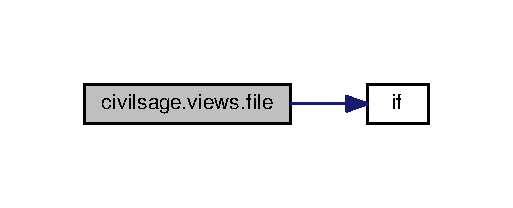
\includegraphics[width=246pt]{namespacecivilsage_1_1views_a32de127956738677913352a2db84ecdb_cgraph}
\end{center}
\end{figure}


\hypertarget{namespacecivilsage_1_1views_a7b4fd4478a312ce8e35a192159c59de9}{}\index{civilsage\+::views@{civilsage\+::views}!index@{index}}
\index{index@{index}!civilsage\+::views@{civilsage\+::views}}
\subsubsection[{index(request)}]{\setlength{\rightskip}{0pt plus 5cm}def civilsage.\+views.\+index (
\begin{DoxyParamCaption}
\item[{}]{request}
\end{DoxyParamCaption}
)}\label{namespacecivilsage_1_1views_a7b4fd4478a312ce8e35a192159c59de9}
\begin{DoxyVerb}first veiw created by rendering html page
from templete
...
\end{DoxyVerb}
 
\begin{DoxyCode}
14 \textcolor{keyword}{def }\hyperlink{namespacecivilsage_1_1views_a7b4fd4478a312ce8e35a192159c59de9}{index}(request):
15     \textcolor{stringliteral}{"""}
16 \textcolor{stringliteral}{    first veiw created by rendering html page}
17 \textcolor{stringliteral}{    from templete}
18 \textcolor{stringliteral}{    ...}
19 \textcolor{stringliteral}{    """}
20 
21     \textcolor{keywordflow}{return} render(request, \textcolor{stringliteral}{'civilsage/index.html'})
22 
\end{DoxyCode}
\hypertarget{namespacecivilsage_1_1views_aed47fb0740a2fa14693f697905788719}{}\index{civilsage\+::views@{civilsage\+::views}!last@{last}}
\index{last@{last}!civilsage\+::views@{civilsage\+::views}}
\subsubsection[{last(request)}]{\setlength{\rightskip}{0pt plus 5cm}def civilsage.\+views.\+last (
\begin{DoxyParamCaption}
\item[{}]{request}
\end{DoxyParamCaption}
)}\label{namespacecivilsage_1_1views_aed47fb0740a2fa14693f697905788719}
\begin{DoxyVerb}This function gets request from matix.html and
gives pdf as output to user
...
\end{DoxyVerb}
 
\begin{DoxyCode}
71 \textcolor{keyword}{def }\hyperlink{namespacecivilsage_1_1views_aed47fb0740a2fa14693f697905788719}{last}(request):
72     \textcolor{stringliteral}{"""}
73 \textcolor{stringliteral}{}
74 \textcolor{stringliteral}{    This function gets request from matix.html and}
75 \textcolor{stringliteral}{    gives pdf as output to user}
76 \textcolor{stringliteral}{    ...}
77 \textcolor{stringliteral}{    """}
78 
79     message=\textcolor{stringliteral}{'error occured please fill again'}
80 
81     \textcolor{comment}{#dictionary of all input tags}
82     lists = \{\textcolor{stringliteral}{'Soil\_type'}:\textcolor{stringliteral}{''},\textcolor{stringliteral}{'Number\_of\_storeys'}:\textcolor{stringliteral}{''}
83     ,\textcolor{stringliteral}{'Importance\_factor'}:\textcolor{stringliteral}{''},\textcolor{stringliteral}{'Response\_reduction\_factor'}:\textcolor{stringliteral}{''}
84     ,\textcolor{stringliteral}{'Zone\_factor'}:\textcolor{stringliteral}{''},\textcolor{stringliteral}{'Gravity\_acceleration'}:\textcolor{stringliteral}{''}
85     ,\textcolor{stringliteral}{'Modes\_considered'}:\textcolor{stringliteral}{''}\}
86     \textcolor{keywordflow}{try}:
87 
88         \textcolor{comment}{#name of directory of specific user}
89         name=\textcolor{stringliteral}{''}
90 
91         \textcolor{comment}{#getting input using tags}
92         \textcolor{keywordflow}{for} var \textcolor{keywordflow}{in} lists.keys():
93             lists[var]=request.session.get(var)
94             name=name+str(lists[var])
95         print(request.session.get(var))
96         command=\textcolor{stringliteral}{'cp -r sagemath '}+name
97         os.popen(command)
98 
99         \textcolor{comment}{#opening file for writing}
100         command=name+\textcolor{stringliteral}{'/input.sage'}
101         file = open(command, \textcolor{stringliteral}{'w'})
102 
103         \textcolor{comment}{#writing variables in input.sage file with syntax of sage}
104         \textcolor{keywordflow}{for} var \textcolor{keywordflow}{in} lists.keys():
105             file.write(var)
106             file.write(\textcolor{stringliteral}{'='})
107             file.write(lists[var])
108             file.write(\textcolor{stringliteral}{'\(\backslash\)n'})
109         file.close()
110 
111         \textcolor{comment}{#getting numbers of storeys}
112         num = request.session.get(\textcolor{stringliteral}{'Number\_of\_storeys'})
113 
114         \textcolor{comment}{#opening input.sage to append remaining inputs}
115         command=name+\textcolor{stringliteral}{'/input.sage'}
116         file=open(command,\textcolor{stringliteral}{'a'})
117 
118         \textcolor{comment}{#list of basic tags}
119         var = [\textcolor{stringliteral}{'mass'},\textcolor{stringliteral}{'Height\_storey'},\textcolor{stringliteral}{'Stiffness\_storey'}]
120 
121         \textcolor{comment}{#writing matix into sage file}
122         \textcolor{keywordflow}{for} j \textcolor{keywordflow}{in} var:
123             file.write(j)
124             file.write(\textcolor{stringliteral}{'=matrix(['})
125 
126             \textcolor{comment}{#writing elements of matix}
127             \textcolor{keywordflow}{for} i \textcolor{keywordflow}{in} range(int(num)):
128 
129                 \textcolor{comment}{#creating input tags}
130                 temp = j+str(i)
131                 file.write(\textcolor{stringliteral}{'['})
132 
133                 \textcolor{comment}{#getting input from tags}
134                 d=request.POST.get(temp)
135                 file.write(d)
136                 file.write(\textcolor{stringliteral}{']'})
137 
138                 \textcolor{comment}{#condition to check last element}
139                 \hyperlink{bootstrap_8min_8js_ac2d69f5011896c6ed4a54e0dd36f6334}{if}( i!=int(num)-1):
140                     file.write(\textcolor{stringliteral}{','})
141             file.write(\textcolor{stringliteral}{'])\(\backslash\)n'})
142         file.close()
143 
144         \textcolor{comment}{#creating and writing sh file for background processing}
145         command=name+\textcolor{stringliteral}{'/civil.sh'}
146         file=open(command,\textcolor{stringliteral}{'w'})
147         command=\textcolor{stringliteral}{'cd '}+name
148         file.write(command)
149         file.write(\textcolor{stringliteral}{'\(\backslash\)nlatex civil.tex\(\backslash\)nsage civil.sagetex.sage\(\backslash\)n'})
150         file.write(\textcolor{stringliteral}{'pdflatex civil.tex\(\backslash\)n'})
151         file.close()
152 
153         \textcolor{comment}{#calling sh file for background processing}
154         command=\textcolor{stringliteral}{'sh '}+name+\textcolor{stringliteral}{'/civil.sh'}
155         os.system(command)
156 
157         \textcolor{comment}{#opening creted pdf to display to user}
158         command=name+\textcolor{stringliteral}{'/civil.pdf'}
159         f=open(command)
160 
161         \textcolor{comment}{#sending pdf as response}
162         response = HttpResponse(f,content\_type=\textcolor{stringliteral}{'application/pdf'})
163         response[\textcolor{stringliteral}{'Content-Disposition'}] = \textcolor{stringliteral}{'attachment; filename="civil.pdf"'}
164         \hyperlink{bootstrap_8min_8js_ac2d69f5011896c6ed4a54e0dd36f6334}{if}(request.GET.get(\textcolor{stringliteral}{'email\_id'})):
165             email\_id=request.POST.get(\textcolor{stringliteral}{'email\_id'})
166             user\_email = EmailMessage(\textcolor{stringliteral}{'Your PDF is ready!'},
167             \textcolor{stringliteral}{'You have is ready'}, to=[email\_id])
168             user\_email.attach\_file(command)
169             user\_email.send()
170             command=\textcolor{stringliteral}{'rm -rf '}+name
171             os.system(command)
172             \textcolor{keywordflow}{return} render(request, \textcolor{stringliteral}{"civilsage/index.html"}, \{\})
173         \textcolor{keywordflow}{else}:
174 
175             \textcolor{comment}{#deleting temperary files}
176             command=\textcolor{stringliteral}{'rm -rf '}+name
177             os.system(command)
178             \textcolor{keywordflow}{return} response
179     \textcolor{keywordflow}{except}:
180         \textcolor{keywordflow}{return} render(request, \textcolor{stringliteral}{"civilsage/matrix.html"},
181         \{\textcolor{stringliteral}{'message'}:message,\textcolor{stringliteral}{'email\_get'}:request.session.get(\textcolor{stringliteral}{'email\_get'})\})
182 
183 
\end{DoxyCode}


Here is the call graph for this function\+:
\nopagebreak
\begin{figure}[H]
\begin{center}
\leavevmode
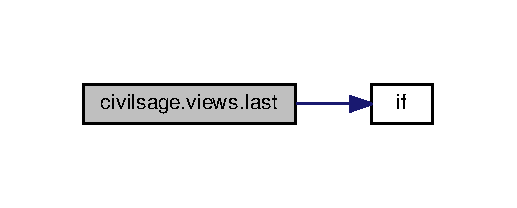
\includegraphics[width=248pt]{namespacecivilsage_1_1views_aed47fb0740a2fa14693f697905788719_cgraph}
\end{center}
\end{figure}


\hypertarget{namespacecivilsage_1_1views_a8b58c93a9c82e84143c43dafaa744a4b}{}\index{civilsage\+::views@{civilsage\+::views}!matrix@{matrix}}
\index{matrix@{matrix}!civilsage\+::views@{civilsage\+::views}}
\subsubsection[{matrix(request)}]{\setlength{\rightskip}{0pt plus 5cm}def civilsage.\+views.\+matrix (
\begin{DoxyParamCaption}
\item[{}]{request}
\end{DoxyParamCaption}
)}\label{namespacecivilsage_1_1views_a8b58c93a9c82e84143c43dafaa744a4b}
\begin{DoxyVerb}This function display matrix for input from user and take
response from index veiw and write input taken through index.html
and write in input.sage file
...
\end{DoxyVerb}
 
\begin{DoxyCode}
23 \textcolor{keyword}{def }\hyperlink{namespacecivilsage_1_1views_a8b58c93a9c82e84143c43dafaa744a4b}{matrix}(request):
24     \textcolor{stringliteral}{"""}
25 \textcolor{stringliteral}{    This function display matrix for input from user and take}
26 \textcolor{stringliteral}{    response from index veiw and write input taken through index.html}
27 \textcolor{stringliteral}{    and write in input.sage file}
28 \textcolor{stringliteral}{    ...}
29 \textcolor{stringliteral}{    """}
30 
31     \textcolor{keywordflow}{try}:
32         \textcolor{comment}{#dictionary of all input tags}
33         lists = \{\textcolor{stringliteral}{'Soil\_type'}:\textcolor{stringliteral}{''},\textcolor{stringliteral}{'Number\_of\_storeys'}:\textcolor{stringliteral}{''}
34         ,\textcolor{stringliteral}{'Importance\_factor'}:\textcolor{stringliteral}{''},\textcolor{stringliteral}{'Response\_reduction\_factor'}:\textcolor{stringliteral}{''}
35         ,\textcolor{stringliteral}{'Zone\_factor'}:\textcolor{stringliteral}{''},\textcolor{stringliteral}{'Gravity\_acceleration'}:\textcolor{stringliteral}{''}
36         ,\textcolor{stringliteral}{'Modes\_considered'}:\textcolor{stringliteral}{''},\textcolor{stringliteral}{'email\_get'}:\textcolor{stringliteral}{''}\}
37 
38         \textcolor{comment}{#name of directory of specific user}
39         name = \textcolor{stringliteral}{''}
40 
41         \textcolor{comment}{#getting input using tags and sending it as response}
42         \textcolor{keywordflow}{for} var \textcolor{keywordflow}{in} lists.keys():
43             request.session[var] = request.POST.get(var)
44 
45         \textcolor{comment}{#creating directory from base directory}
46         lists[\textcolor{stringliteral}{'Number\_of\_storeys'}] = request.POST.get(\textcolor{stringliteral}{'Number\_of\_storeys'})
47 
48         \textcolor{comment}{#making list for iteratation in templete}
49         number\_of\_storeys = list()
50         \textcolor{keywordflow}{for} a \textcolor{keywordflow}{in} range(int(lists[\textcolor{stringliteral}{'Number\_of\_storeys'}])):
51             number\_of\_storeys.append(\textcolor{stringliteral}{'a'})
52 
53         \textcolor{comment}{#calling differnet veiws based on option whether}
54         \textcolor{comment}{#user want to upload matrix value through file or}
55         \textcolor{comment}{#manually}
56 
57         \hyperlink{bootstrap_8min_8js_ac2d69f5011896c6ed4a54e0dd36f6334}{if}(request.POST.get(\textcolor{stringliteral}{'through\_file'})==\textcolor{stringliteral}{'Y'}):
58             \textcolor{keywordflow}{return} render( request,\textcolor{stringliteral}{'civilsage/file.html'}
59             ,\{\textcolor{stringliteral}{'number\_of\_storeys'}: number\_of\_storeys,
60             \textcolor{stringliteral}{'email\_get'}: request.POST.get(\textcolor{stringliteral}{'email\_get'})\})
61         \textcolor{keywordflow}{else}:
62             \textcolor{keywordflow}{return} render( request,\textcolor{stringliteral}{'civilsage/matrix.html'}
63             ,\{\textcolor{stringliteral}{'number\_of\_storeys'}: number\_of\_storeys,
64             \textcolor{stringliteral}{'email\_get'}: request.POST.get(\textcolor{stringliteral}{'email\_get'}) \})
65     \textcolor{keywordflow}{except}:
66         \textcolor{keywordflow}{return} render(request, \textcolor{stringliteral}{'civilsage/index.html'}
67         ,\{\textcolor{stringliteral}{'message'}:\textcolor{stringliteral}{'please fill again'}\})
68 
69 
70 
\end{DoxyCode}


Here is the call graph for this function\+:
\nopagebreak
\begin{figure}[H]
\begin{center}
\leavevmode
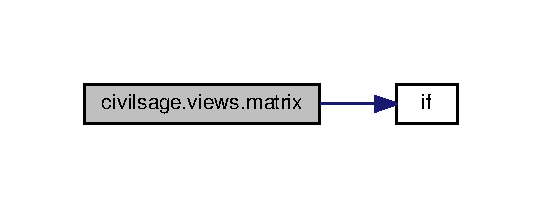
\includegraphics[width=260pt]{namespacecivilsage_1_1views_a8b58c93a9c82e84143c43dafaa744a4b_cgraph}
\end{center}
\end{figure}



\hypertarget{namespaceinitial__file}{}\section{initial\+\_\+file Namespace Reference}
\label{namespaceinitial__file}\index{initial\+\_\+file@{initial\+\_\+file}}
\subsection*{Functions}
\begin{DoxyCompactItemize}
\item 
def \hyperlink{namespaceinitial__file_a105b1aa7bf4db853b6f4d064ed224030}{pdfemail} ()
\end{DoxyCompactItemize}


\subsection{Function Documentation}
\hypertarget{namespaceinitial__file_a105b1aa7bf4db853b6f4d064ed224030}{}\index{initial\+\_\+file@{initial\+\_\+file}!pdfemail@{pdfemail}}
\index{pdfemail@{pdfemail}!initial\+\_\+file@{initial\+\_\+file}}
\subsubsection[{pdfemail()}]{\setlength{\rightskip}{0pt plus 5cm}def initial\+\_\+file.\+pdfemail (
\begin{DoxyParamCaption}
{}
\end{DoxyParamCaption}
)}\label{namespaceinitial__file_a105b1aa7bf4db853b6f4d064ed224030}


Definition at line 3 of file initial\+\_\+file.\+py.


\begin{DoxyCode}
3 \textcolor{keyword}{def }\hyperlink{namespaceinitial__file_a105b1aa7bf4db853b6f4d064ed224030}{pdfemail}():
4     os.system(\textcolor{stringliteral}{'sage sagemath/input.sage'})
5     
6 \end{DoxyCode}

\hypertarget{namespaceinput}{}\section{input Namespace Reference}
\label{namespaceinput}\index{input@{input}}
\subsection*{Variables}
\begin{DoxyCompactItemize}
\item 
tuple \hyperlink{namespaceinput_a221dbe0b6723929966d68d807eb5b2db}{\+\_\+sage\+\_\+const\+\_\+1} = Integer(1)
\item 
\hyperlink{namespaceinput_a6221ae01cf2fb9e8cd22204749785a0e}{Soil\+\_\+type} = \hyperlink{namespaceinput_a221dbe0b6723929966d68d807eb5b2db}{\+\_\+sage\+\_\+const\+\_\+1}
\item 
\hyperlink{namespaceinput_a0840d963ea24db338f3ab4457defb494}{Importance\+\_\+factor} = \+\_\+sage\+\_\+const\+\_\+1p5
\item 
\hyperlink{namespaceinput_a10237b312ba44e8c8090db86059c5803}{Number\+\_\+of\+\_\+storeys} = \+\_\+sage\+\_\+const\+\_\+4
\item 
\hyperlink{namespaceinput_a55ab15c1c171513e99332aa50c723764}{Gravity\+\_\+acceleration} = \+\_\+sage\+\_\+const\+\_\+9p8
\item 
\hyperlink{namespaceinput_adb7aca4735796aaa4a46456d3edeac2e}{Modes\+\_\+considered} = \+\_\+sage\+\_\+const\+\_\+4
\item 
\hyperlink{namespaceinput_aa6d0078a6d934c0d515d85059525e938}{Response\+\_\+reduction\+\_\+factor} = \+\_\+sage\+\_\+const\+\_\+1p5
\item 
\hyperlink{namespaceinput_aeea70e58ec9bb0d3d6c4363867eb0f82}{Zone\+\_\+factor} = \+\_\+sage\+\_\+const\+\_\+p1
\item 
tuple \hyperlink{namespaceinput_af91e2c1a9ecd07a9c8dcf3a5fc8b2b60}{mass} = matrix(\mbox{[}\mbox{[}\+\_\+sage\+\_\+const\+\_\+23 \mbox{]},\mbox{[}\+\_\+sage\+\_\+const\+\_\+23 \mbox{]},\mbox{[}\+\_\+sage\+\_\+const\+\_\+32 \mbox{]},\mbox{[}\+\_\+sage\+\_\+const\+\_\+34 \mbox{]}\mbox{]})
\item 
tuple \hyperlink{namespaceinput_a01ad5b8730285b6aaebb2bc3f3fc0894}{Height\+\_\+storey} = matrix(\mbox{[}\mbox{[}\+\_\+sage\+\_\+const\+\_\+44 \mbox{]},\mbox{[}\+\_\+sage\+\_\+const\+\_\+44 \mbox{]},\mbox{[}\+\_\+sage\+\_\+const\+\_\+23 \mbox{]},\mbox{[}\+\_\+sage\+\_\+const\+\_\+34 \mbox{]},\mbox{]})
\item 
tuple \hyperlink{namespaceinput_a3853184afbe677b2a218690766c4f5e4}{Stiffness\+\_\+storey} = matrix(\mbox{[}\mbox{[}\+\_\+sage\+\_\+const\+\_\+34 \mbox{]},\mbox{[}\+\_\+sage\+\_\+const\+\_\+34 \mbox{]},\mbox{[}\+\_\+sage\+\_\+const\+\_\+23 \mbox{]},\mbox{[}\+\_\+sage\+\_\+const\+\_\+34 \mbox{]},\mbox{]})
\end{DoxyCompactItemize}


\subsection{Variable Documentation}
\hypertarget{namespaceinput_a221dbe0b6723929966d68d807eb5b2db}{}\index{input@{input}!\+\_\+sage\+\_\+const\+\_\+1@{\+\_\+sage\+\_\+const\+\_\+1}}
\index{\+\_\+sage\+\_\+const\+\_\+1@{\+\_\+sage\+\_\+const\+\_\+1}!input@{input}}
\subsubsection[{\+\_\+sage\+\_\+const\+\_\+1}]{\setlength{\rightskip}{0pt plus 5cm}tuple input.\+\_\+sage\+\_\+const\+\_\+1 = Integer(1)}\label{namespaceinput_a221dbe0b6723929966d68d807eb5b2db}


Definition at line 3 of file input.\+sage.\+py.

\hypertarget{namespaceinput_a55ab15c1c171513e99332aa50c723764}{}\index{input@{input}!Gravity\+\_\+acceleration@{Gravity\+\_\+acceleration}}
\index{Gravity\+\_\+acceleration@{Gravity\+\_\+acceleration}!input@{input}}
\subsubsection[{Gravity\+\_\+acceleration}]{\setlength{\rightskip}{0pt plus 5cm}input.\+Gravity\+\_\+acceleration = \+\_\+sage\+\_\+const\+\_\+9p8}\label{namespaceinput_a55ab15c1c171513e99332aa50c723764}


Definition at line 7 of file input.\+sage.\+py.

\hypertarget{namespaceinput_a01ad5b8730285b6aaebb2bc3f3fc0894}{}\index{input@{input}!Height\+\_\+storey@{Height\+\_\+storey}}
\index{Height\+\_\+storey@{Height\+\_\+storey}!input@{input}}
\subsubsection[{Height\+\_\+storey}]{\setlength{\rightskip}{0pt plus 5cm}tuple input.\+Height\+\_\+storey = matrix(\mbox{[}\mbox{[}\+\_\+sage\+\_\+const\+\_\+44 \mbox{]},\mbox{[}\+\_\+sage\+\_\+const\+\_\+44 \mbox{]},\mbox{[}\+\_\+sage\+\_\+const\+\_\+23 \mbox{]},\mbox{[}\+\_\+sage\+\_\+const\+\_\+34 \mbox{]},\mbox{]})}\label{namespaceinput_a01ad5b8730285b6aaebb2bc3f3fc0894}


Definition at line 12 of file input.\+sage.\+py.

\hypertarget{namespaceinput_a0840d963ea24db338f3ab4457defb494}{}\index{input@{input}!Importance\+\_\+factor@{Importance\+\_\+factor}}
\index{Importance\+\_\+factor@{Importance\+\_\+factor}!input@{input}}
\subsubsection[{Importance\+\_\+factor}]{\setlength{\rightskip}{0pt plus 5cm}input.\+Importance\+\_\+factor = \+\_\+sage\+\_\+const\+\_\+1p5}\label{namespaceinput_a0840d963ea24db338f3ab4457defb494}


Definition at line 5 of file input.\+sage.\+py.

\hypertarget{namespaceinput_af91e2c1a9ecd07a9c8dcf3a5fc8b2b60}{}\index{input@{input}!mass@{mass}}
\index{mass@{mass}!input@{input}}
\subsubsection[{mass}]{\setlength{\rightskip}{0pt plus 5cm}tuple input.\+mass = matrix(\mbox{[}\mbox{[}\+\_\+sage\+\_\+const\+\_\+23 \mbox{]},\mbox{[}\+\_\+sage\+\_\+const\+\_\+23 \mbox{]},\mbox{[}\+\_\+sage\+\_\+const\+\_\+32 \mbox{]},\mbox{[}\+\_\+sage\+\_\+const\+\_\+34 \mbox{]}\mbox{]})}\label{namespaceinput_af91e2c1a9ecd07a9c8dcf3a5fc8b2b60}


Definition at line 11 of file input.\+sage.\+py.

\hypertarget{namespaceinput_adb7aca4735796aaa4a46456d3edeac2e}{}\index{input@{input}!Modes\+\_\+considered@{Modes\+\_\+considered}}
\index{Modes\+\_\+considered@{Modes\+\_\+considered}!input@{input}}
\subsubsection[{Modes\+\_\+considered}]{\setlength{\rightskip}{0pt plus 5cm}input.\+Modes\+\_\+considered = \+\_\+sage\+\_\+const\+\_\+4}\label{namespaceinput_adb7aca4735796aaa4a46456d3edeac2e}


Definition at line 8 of file input.\+sage.\+py.

\hypertarget{namespaceinput_a10237b312ba44e8c8090db86059c5803}{}\index{input@{input}!Number\+\_\+of\+\_\+storeys@{Number\+\_\+of\+\_\+storeys}}
\index{Number\+\_\+of\+\_\+storeys@{Number\+\_\+of\+\_\+storeys}!input@{input}}
\subsubsection[{Number\+\_\+of\+\_\+storeys}]{\setlength{\rightskip}{0pt plus 5cm}input.\+Number\+\_\+of\+\_\+storeys = \+\_\+sage\+\_\+const\+\_\+4}\label{namespaceinput_a10237b312ba44e8c8090db86059c5803}


Definition at line 6 of file input.\+sage.\+py.

\hypertarget{namespaceinput_aa6d0078a6d934c0d515d85059525e938}{}\index{input@{input}!Response\+\_\+reduction\+\_\+factor@{Response\+\_\+reduction\+\_\+factor}}
\index{Response\+\_\+reduction\+\_\+factor@{Response\+\_\+reduction\+\_\+factor}!input@{input}}
\subsubsection[{Response\+\_\+reduction\+\_\+factor}]{\setlength{\rightskip}{0pt plus 5cm}input.\+Response\+\_\+reduction\+\_\+factor = \+\_\+sage\+\_\+const\+\_\+1p5}\label{namespaceinput_aa6d0078a6d934c0d515d85059525e938}


Definition at line 9 of file input.\+sage.\+py.

\hypertarget{namespaceinput_a6221ae01cf2fb9e8cd22204749785a0e}{}\index{input@{input}!Soil\+\_\+type@{Soil\+\_\+type}}
\index{Soil\+\_\+type@{Soil\+\_\+type}!input@{input}}
\subsubsection[{Soil\+\_\+type}]{\setlength{\rightskip}{0pt plus 5cm}input.\+Soil\+\_\+type = {\bf \+\_\+sage\+\_\+const\+\_\+1}}\label{namespaceinput_a6221ae01cf2fb9e8cd22204749785a0e}


Definition at line 4 of file input.\+sage.\+py.

\hypertarget{namespaceinput_a3853184afbe677b2a218690766c4f5e4}{}\index{input@{input}!Stiffness\+\_\+storey@{Stiffness\+\_\+storey}}
\index{Stiffness\+\_\+storey@{Stiffness\+\_\+storey}!input@{input}}
\subsubsection[{Stiffness\+\_\+storey}]{\setlength{\rightskip}{0pt plus 5cm}tuple input.\+Stiffness\+\_\+storey = matrix(\mbox{[}\mbox{[}\+\_\+sage\+\_\+const\+\_\+34 \mbox{]},\mbox{[}\+\_\+sage\+\_\+const\+\_\+34 \mbox{]},\mbox{[}\+\_\+sage\+\_\+const\+\_\+23 \mbox{]},\mbox{[}\+\_\+sage\+\_\+const\+\_\+34 \mbox{]},\mbox{]})}\label{namespaceinput_a3853184afbe677b2a218690766c4f5e4}


Definition at line 13 of file input.\+sage.\+py.

\hypertarget{namespaceinput_aeea70e58ec9bb0d3d6c4363867eb0f82}{}\index{input@{input}!Zone\+\_\+factor@{Zone\+\_\+factor}}
\index{Zone\+\_\+factor@{Zone\+\_\+factor}!input@{input}}
\subsubsection[{Zone\+\_\+factor}]{\setlength{\rightskip}{0pt plus 5cm}input.\+Zone\+\_\+factor = \+\_\+sage\+\_\+const\+\_\+p1}\label{namespaceinput_aeea70e58ec9bb0d3d6c4363867eb0f82}


Definition at line 10 of file input.\+sage.\+py.


\hypertarget{namespacemain}{}\section{main Namespace Reference}
\label{namespacemain}\index{main@{main}}
\subsection*{Functions}
\begin{DoxyCompactItemize}
\item 
def \hyperlink{namespacemain_a4f60afd2426ee9409955e4352b3f0486}{fun\+Saog} (soil\+Type, time\+Prd)
\begin{DoxyCompactList}\small\item\em function to pick values according to type of soil selected \end{DoxyCompactList}\end{DoxyCompactItemize}
\subsection*{Variables}
\begin{DoxyCompactItemize}
\item 
tuple \hyperlink{namespacemain_ad85d7913c0e40b9e1f30e64611a0fafa}{\+\_\+sage\+\_\+const\+\_\+2} = Integer(2)
\item 
tuple \hyperlink{namespacemain_ad7b051da0e829aff37fef1e171e37fa3}{Level\+\_\+floor} = zero\+\_\+matrix(Q\+Q,Number\+\_\+of\+\_\+storeys,\+\_\+sage\+\_\+const\+\_\+1 )
\item 
tuple \hyperlink{namespacemain_a0011be18dbc87087d6aaf28802f121c0}{Stiffness\+\_\+matrix} = zero\+\_\+matrix(Q\+Q,Number\+\_\+of\+\_\+storeys,Number\+\_\+of\+\_\+storeys)
\item 
tuple \hyperlink{namespacemain_af76005101c339a32cd5d37ba82ee072c}{w} = var(\textquotesingle{}w\textquotesingle{})
\item 
tuple \hyperlink{namespacemain_a1787a37505189f764069a45071189112}{q} = \hyperlink{namespacemain_a0011be18dbc87087d6aaf28802f121c0}{Stiffness\+\_\+matrix}-\/(\hyperlink{namespacemain_af76005101c339a32cd5d37ba82ee072c}{w}$\ast$$\ast$\hyperlink{namespacemain_ad85d7913c0e40b9e1f30e64611a0fafa}{\+\_\+sage\+\_\+const\+\_\+2} )
\item 
tuple \hyperlink{namespacemain_ad101f166a53497f04b37636bcadbfe65}{A} = \hyperlink{namespacemain_a0011be18dbc87087d6aaf28802f121c0}{Stiffness\+\_\+matrix}$\ast$Mass.\+inverse()
\item 
tuple \hyperlink{namespacemain_a63066086ca439ff34de16475b00387f5}{Omega\+\_\+square} = A.\+eigenvalues()
\item 
tuple \hyperlink{namespacemain_af44dcb60e61649c65257466d65b4d548}{Omega} = zero\+\_\+matrix(R\+R,Number\+\_\+of\+\_\+storeys,\+\_\+sage\+\_\+const\+\_\+1 )
\item 
tuple \hyperlink{namespacemain_a6bf4b8266bcb3b4f390149620fea3d6c}{Time\+\_\+period} = zero\+\_\+matrix(R\+R,Number\+\_\+of\+\_\+storeys,\+\_\+sage\+\_\+const\+\_\+1 )
\item 
tuple \hyperlink{namespacemain_a2d5b336e3b2f7d2e14f04fa3cc413457}{z} = A.\+eigenvectors\+\_\+left()
\item 
tuple \hyperlink{namespacemain_a00488f5887e168f7781b6fb94dd08518}{J} = zero\+\_\+matrix(R\+R,Number\+\_\+of\+\_\+storeys,\+\_\+sage\+\_\+const\+\_\+1 )
\item 
tuple \hyperlink{namespacemain_a5eac8e4368036ef94463d6e42c1628c5}{X} = zero\+\_\+matrix(R\+R,Number\+\_\+of\+\_\+storeys,Number\+\_\+of\+\_\+storeys)
\item 
tuple \hyperlink{namespacemain_a70551c7fc78da8fdec83fe500056d388}{mid} = \hyperlink{namespacemain_a1787a37505189f764069a45071189112}{q}$\ast$Mass$\ast$q.\+transpose()
\item 
tuple \hyperlink{namespacemain_a936ce857e8e4f4855af1cc5bf2635191}{Modal\+\_\+participation\+\_\+factor} = zero\+\_\+matrix(R\+R,Number\+\_\+of\+\_\+storeys,\+\_\+sage\+\_\+const\+\_\+1 )
\item 
tuple \hyperlink{namespacemain_a176940b2d446033050ac092436f63974}{Modal\+\_\+mass} = zero\+\_\+matrix(R\+R,Number\+\_\+of\+\_\+storeys,\+\_\+sage\+\_\+const\+\_\+1 )
\item 
\hyperlink{namespacemain_a27fb93072b84fd448623807df350f132}{sum\+\_\+modal\+\_\+mass} = \+\_\+sage\+\_\+const\+\_\+0
\item 
list \hyperlink{namespacemain_af6e3698b7f50fc004eb759d7c447fdb3}{m} = \hyperlink{namespacemain_a5eac8e4368036ef94463d6e42c1628c5}{X}\mbox{[}\hyperlink{L02_2main_8m_ac86694252f8dfdb19aaeadc4b7c342c6}{j},\+:\mbox{]}
\item 
list \hyperlink{namespacemain_add7e0394c94a2e2115aff785eb6995e3}{P1} = P1+Mass\mbox{[}\hyperlink{L02_2main_8m_a6dbbc96f4222af2f6c18c8e60f41726b}{i}\mbox{]}
\item 
list \hyperlink{namespacemain_a1b83b7a3849a8e1c84b9906c45625fec}{P2} = P2+Mass\mbox{[}\hyperlink{L02_2main_8m_a6dbbc96f4222af2f6c18c8e60f41726b}{i}\mbox{]}
\item 
tuple \hyperlink{namespacemain_ae18df6a00aee4516c7ad8961b666e2a3}{X\+X} = X.\+transpose()
\item 
tuple \hyperlink{namespacemain_ab273c2ae46514d6ec3d905c30cbb5a1b}{Modal\+\_\+contribution} = zero\+\_\+matrix(R\+R,Number\+\_\+of\+\_\+storeys,\+\_\+sage\+\_\+const\+\_\+1 )
\item 
\hyperlink{namespacemain_a9d22ac077c22a97b1b095068a1500d16}{Modes\+\_\+considered} = Number\+\_\+of\+\_\+storeys
\item 
string \hyperlink{namespacemain_a52e65712caa18dade1326ad4efeebfa1}{Type\+\_\+of\+\_\+soil} = \textquotesingle{}\textquotesingle{}
\item 
tuple \hyperlink{namespacemain_ac3a509169246622b50fc23d809d30833}{Sa\+\_\+by\+\_\+g} = zero\+\_\+matrix(R\+R,Number\+\_\+of\+\_\+storeys,\+\_\+sage\+\_\+const\+\_\+1 )
\item 
tuple \hyperlink{namespacemain_a49b10c1530f56b101c4cc17b20fb1973}{A\+\_\+h} = zero\+\_\+matrix(R\+R,Number\+\_\+of\+\_\+storeys,Number\+\_\+of\+\_\+storeys)
\item 
tuple \hyperlink{namespacemain_a0caf610899fee63b00acb7cce7c804d7}{Design\+\_\+lateral\+\_\+force} = zero\+\_\+matrix(R\+R,Number\+\_\+of\+\_\+storeys,\hyperlink{namespacemain_a9d22ac077c22a97b1b095068a1500d16}{Modes\+\_\+considered})
\item 
tuple \hyperlink{namespacemain_a9e135aea550f8ea419857f817a196d56}{Peak\+\_\+shear\+\_\+force} = zero\+\_\+matrix(R\+R,Number\+\_\+of\+\_\+storeys,\hyperlink{namespacemain_a9d22ac077c22a97b1b095068a1500d16}{Modes\+\_\+considered})
\item 
tuple \hyperlink{namespacemain_aaa52e7055409dcf0785880422294a704}{Storey\+\_\+shear\+\_\+force} = zero\+\_\+matrix(R\+R,Number\+\_\+of\+\_\+storeys,\+\_\+sage\+\_\+const\+\_\+1 )
\item 
tuple \hyperlink{namespacemain_ab6dd9cc05fd903a9da8b9734c44fef57}{Storey\+\_\+shear\+\_\+force2} = zero\+\_\+matrix(R\+R,Number\+\_\+of\+\_\+storeys,\+\_\+sage\+\_\+const\+\_\+1 )
\item 
tuple \hyperlink{namespacemain_aa91561fad2579200e566fa01f3cbc359}{Force} = zero\+\_\+matrix(R\+R,Number\+\_\+of\+\_\+storeys,\+\_\+sage\+\_\+const\+\_\+1 )
\item 
tuple \hyperlink{namespacemain_ad403610ba53df02f8dfaff8dd64227b3}{P} = zero\+\_\+matrix(R\+R,\hyperlink{namespacemain_a9d22ac077c22a97b1b095068a1500d16}{Modes\+\_\+considered},\hyperlink{namespacemain_a9d22ac077c22a97b1b095068a1500d16}{Modes\+\_\+considered})
\item 
tuple \hyperlink{namespacemain_a6ae8768d11174f5baf9febc5244d6f06}{B} = zero\+\_\+matrix(R\+R,\hyperlink{namespacemain_a9d22ac077c22a97b1b095068a1500d16}{Modes\+\_\+considered},\hyperlink{namespacemain_a9d22ac077c22a97b1b095068a1500d16}{Modes\+\_\+considered})
\item 
list \hyperlink{namespacemain_a4760f4121f66000c5570f75176649cb8}{r} = \hyperlink{namespacemain_af44dcb60e61649c65257466d65b4d548}{Omega}\mbox{[}\hyperlink{L02_2main_8m_ac86694252f8dfdb19aaeadc4b7c342c6}{j},\+\_\+sage\+\_\+const\+\_\+0 \mbox{]}
\item 
list \hyperlink{namespacemain_ab1e783015bffd2e1d395a9099143d967}{b} = \+\_\+sage\+\_\+const\+\_\+1+\hyperlink{namespacemain_a6ae8768d11174f5baf9febc5244d6f06}{B}\mbox{[}\hyperlink{L02_2main_8m_a6dbbc96f4222af2f6c18c8e60f41726b}{i},\hyperlink{L02_2main_8m_ac86694252f8dfdb19aaeadc4b7c342c6}{j}\mbox{]}
\item 
tuple \hyperlink{namespacemain_aa7f4fe671f919f7f067f9337ef9e02c0}{e} = (\+\_\+sage\+\_\+const\+\_\+1 -\/\hyperlink{namespacemain_a6ae8768d11174f5baf9febc5244d6f06}{B}\mbox{[}\hyperlink{L02_2main_8m_a6dbbc96f4222af2f6c18c8e60f41726b}{i},\hyperlink{L02_2main_8m_ac86694252f8dfdb19aaeadc4b7c342c6}{j}\mbox{]}$\ast$$\ast$\hyperlink{namespacemain_ad85d7913c0e40b9e1f30e64611a0fafa}{\+\_\+sage\+\_\+const\+\_\+2} )
\item 
tuple \hyperlink{namespacemain_a712447a841ce148ad2d1210e57dc7894}{Lateral\+\_\+force} = zero\+\_\+matrix(R\+R,Number\+\_\+of\+\_\+storeys,\+\_\+sage\+\_\+const\+\_\+1 )
\item 
list \hyperlink{namespacemain_a027916efc284622d928c1d8383917f6d}{l} = \hyperlink{namespacemain_a9e135aea550f8ea419857f817a196d56}{Peak\+\_\+shear\+\_\+force}\mbox{[}\hyperlink{L02_2main_8m_a6dbbc96f4222af2f6c18c8e60f41726b}{i},\+:\mbox{]}
\item 
tuple \hyperlink{namespacemain_ab31fc16b432d2248a6c76c6a18d741d0}{p} = list()
\item 
tuple \hyperlink{namespacemain_aeabbf69db1809807f065c2d1e9a62567}{color} = hue(\+\_\+sage\+\_\+const\+\_\+0p4 + \+\_\+sage\+\_\+const\+\_\+0p6 $\ast$(\hyperlink{L02_2main_8m_a6dbbc96f4222af2f6c18c8e60f41726b}{i}/\+\_\+sage\+\_\+const\+\_\+10 ))
\item 
tuple \hyperlink{namespacemain_ad40f6b3437e83a0385177ac65a317b97}{Graph} = plot(\mbox{[}$\,$\mbox{]})
\item 
list \hyperlink{namespacemain_aa741e0bac28acc57bb99fbe2b14205c7}{storey\+\_\+shear\+\_\+force3} = \hyperlink{namespacemain_aaa52e7055409dcf0785880422294a704}{Storey\+\_\+shear\+\_\+force}\mbox{[}\+:\mbox{]}
\end{DoxyCompactItemize}


\subsection{Function Documentation}
\hypertarget{namespacemain_a4f60afd2426ee9409955e4352b3f0486}{}\index{main@{main}!fun\+Saog@{fun\+Saog}}
\index{fun\+Saog@{fun\+Saog}!main@{main}}
\subsubsection[{fun\+Saog(soil\+Type, time\+Prd)}]{\setlength{\rightskip}{0pt plus 5cm}def main.\+fun\+Saog (
\begin{DoxyParamCaption}
\item[{}]{soil\+Type, }
\item[{}]{time\+Prd}
\end{DoxyParamCaption}
)}\label{namespacemain_a4f60afd2426ee9409955e4352b3f0486}


function to pick values according to type of soil selected 


\begin{DoxyParams}{Parameters}
{\em soil\+Type} & it tells type of soil \\
\hline
{\em time\+Prd} & time period of mode of floor \\
\hline
\end{DoxyParams}
\begin{DoxyReturn}{Returns}
Sag 
\end{DoxyReturn}


Definition at line 18 of file main.\+sage.\+py.


\begin{DoxyCode}
18 \textcolor{keyword}{def }\hyperlink{namespacemain_a4f60afd2426ee9409955e4352b3f0486}{funSaog}(soilType, timePrd):
19 
20   t1 = \_sage\_const\_0 ; t2 = \_sage\_const\_0 ; t3 = \_sage\_const\_0 ; t4 = \_sage\_const\_0 
21   eq3num = \_sage\_const\_0 
22   t2 = \_sage\_const\_0p10 
23   \hyperlink{bootstrap_8min_8js_ac2d69f5011896c6ed4a54e0dd36f6334}{if}(soilType==\textcolor{stringliteral}{'I'}):
24       t3 = \_sage\_const\_0p40 ; eq3num = \_sage\_const\_1p0 
25   \textcolor{keywordflow}{elif} (soilType==\textcolor{stringliteral}{'II'}):
26       t3 = \_sage\_const\_0p55 ; eq3num = \_sage\_const\_1p36 
27   elif(soilType==\textcolor{stringliteral}{'III'}):
28       t3 = \_sage\_const\_0p67 ; eq3num = \_sage\_const\_1p67 
29   \textcolor{keywordflow}{else}:
30       Print(\textcolor{stringliteral}{'Unexpected soil type'})
31   \textcolor{keywordflow}{if} (timePrd < t2):
32       sag = \_sage\_const\_1p  + \_sage\_const\_15  * timePrd
33   elif(timePrd > t3):
34       sag = eq3num / timePrd
35   \textcolor{keywordflow}{else}:
36       sag = \_sage\_const\_2p5 
37   \textcolor{keywordflow}{return} sag
38 
39 \textcolor{stringliteral}{"""main program ... """}
40 
41 \textcolor{comment}{#loading input variables from input.sage}
42 load(\textcolor{stringliteral}{'input.sage'})
43 \textcolor{comment}{#changing style of brackets for latex output}
44 latex.matrix\_delimiters(\textcolor{stringliteral}{"["},\textcolor{stringliteral}{"]"})
45 t=time.clock()
46 \textcolor{comment}{#converting mass in diagonal matrix}
47 Mass=\hyperlink{namespacecivilsage_1_1views_a8b58c93a9c82e84143c43dafaa744a4b}{matrix}(QQ,Number\_of\_storeys,Number\_of\_storeys)
\end{DoxyCode}


Here is the call graph for this function\+:
\nopagebreak
\begin{figure}[H]
\begin{center}
\leavevmode
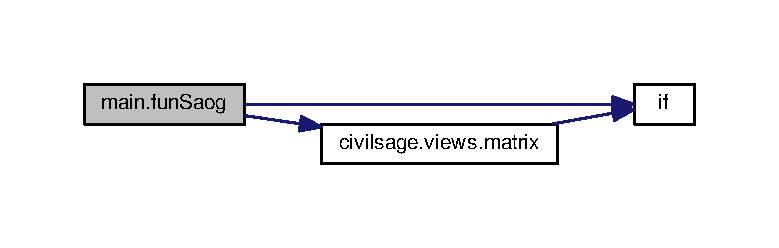
\includegraphics[width=350pt]{namespacemain_a4f60afd2426ee9409955e4352b3f0486_cgraph}
\end{center}
\end{figure}




\subsection{Variable Documentation}
\hypertarget{namespacemain_ad85d7913c0e40b9e1f30e64611a0fafa}{}\index{main@{main}!\+\_\+sage\+\_\+const\+\_\+2@{\+\_\+sage\+\_\+const\+\_\+2}}
\index{\+\_\+sage\+\_\+const\+\_\+2@{\+\_\+sage\+\_\+const\+\_\+2}!main@{main}}
\subsubsection[{\+\_\+sage\+\_\+const\+\_\+2}]{\setlength{\rightskip}{0pt plus 5cm}tuple main.\+\_\+sage\+\_\+const\+\_\+2 = Integer(2)}\label{namespacemain_ad85d7913c0e40b9e1f30e64611a0fafa}


Definition at line 3 of file main.\+sage.\+py.

\hypertarget{namespacemain_ad101f166a53497f04b37636bcadbfe65}{}\index{main@{main}!A@{A}}
\index{A@{A}!main@{main}}
\subsubsection[{A}]{\setlength{\rightskip}{0pt plus 5cm}tuple main.\+A = {\bf Stiffness\+\_\+matrix}$\ast$Mass.\+inverse()}\label{namespacemain_ad101f166a53497f04b37636bcadbfe65}


Definition at line 77 of file main.\+sage.\+py.

\hypertarget{namespacemain_a49b10c1530f56b101c4cc17b20fb1973}{}\index{main@{main}!A\+\_\+h@{A\+\_\+h}}
\index{A\+\_\+h@{A\+\_\+h}!main@{main}}
\subsubsection[{A\+\_\+h}]{\setlength{\rightskip}{0pt plus 5cm}tuple main.\+A\+\_\+h = zero\+\_\+matrix(R\+R,Number\+\_\+of\+\_\+storeys,Number\+\_\+of\+\_\+storeys)}\label{namespacemain_a49b10c1530f56b101c4cc17b20fb1973}


Definition at line 140 of file main.\+sage.\+py.

\hypertarget{namespacemain_a6ae8768d11174f5baf9febc5244d6f06}{}\index{main@{main}!B@{B}}
\index{B@{B}!main@{main}}
\subsubsection[{B}]{\setlength{\rightskip}{0pt plus 5cm}tuple main.\+B = zero\+\_\+matrix(R\+R,{\bf Modes\+\_\+considered},{\bf Modes\+\_\+considered})}\label{namespacemain_a6ae8768d11174f5baf9febc5244d6f06}


Definition at line 190 of file main.\+sage.\+py.

\hypertarget{namespacemain_ab1e783015bffd2e1d395a9099143d967}{}\index{main@{main}!b@{b}}
\index{b@{b}!main@{main}}
\subsubsection[{b}]{\setlength{\rightskip}{0pt plus 5cm}list main.\+b = \+\_\+sage\+\_\+const\+\_\+1+{\bf B}\mbox{[}{\bf i},{\bf j}\mbox{]}}\label{namespacemain_ab1e783015bffd2e1d395a9099143d967}


Definition at line 201 of file main.\+sage.\+py.

\hypertarget{namespacemain_aeabbf69db1809807f065c2d1e9a62567}{}\index{main@{main}!color@{color}}
\index{color@{color}!main@{main}}
\subsubsection[{color}]{\setlength{\rightskip}{0pt plus 5cm}tuple main.\+color = hue(\+\_\+sage\+\_\+const\+\_\+0p4 + \+\_\+sage\+\_\+const\+\_\+0p6 $\ast$({\bf i}/\+\_\+sage\+\_\+const\+\_\+10 ))}\label{namespacemain_aeabbf69db1809807f065c2d1e9a62567}


Definition at line 217 of file main.\+sage.\+py.

\hypertarget{namespacemain_a0caf610899fee63b00acb7cce7c804d7}{}\index{main@{main}!Design\+\_\+lateral\+\_\+force@{Design\+\_\+lateral\+\_\+force}}
\index{Design\+\_\+lateral\+\_\+force@{Design\+\_\+lateral\+\_\+force}!main@{main}}
\subsubsection[{Design\+\_\+lateral\+\_\+force}]{\setlength{\rightskip}{0pt plus 5cm}tuple main.\+Design\+\_\+lateral\+\_\+force = zero\+\_\+matrix(R\+R,Number\+\_\+of\+\_\+storeys,{\bf Modes\+\_\+considered})}\label{namespacemain_a0caf610899fee63b00acb7cce7c804d7}


Definition at line 151 of file main.\+sage.\+py.

\hypertarget{namespacemain_aa7f4fe671f919f7f067f9337ef9e02c0}{}\index{main@{main}!e@{e}}
\index{e@{e}!main@{main}}
\subsubsection[{e}]{\setlength{\rightskip}{0pt plus 5cm}tuple main.\+e = (\+\_\+sage\+\_\+const\+\_\+1 -\/{\bf B}\mbox{[}{\bf i},{\bf j}\mbox{]}$\ast$$\ast${\bf \+\_\+sage\+\_\+const\+\_\+2} )}\label{namespacemain_aa7f4fe671f919f7f067f9337ef9e02c0}


Definition at line 203 of file main.\+sage.\+py.

\hypertarget{namespacemain_aa91561fad2579200e566fa01f3cbc359}{}\index{main@{main}!Force@{Force}}
\index{Force@{Force}!main@{main}}
\subsubsection[{Force}]{\setlength{\rightskip}{0pt plus 5cm}tuple main.\+Force = zero\+\_\+matrix(R\+R,Number\+\_\+of\+\_\+storeys,\+\_\+sage\+\_\+const\+\_\+1 )}\label{namespacemain_aa91561fad2579200e566fa01f3cbc359}


Definition at line 181 of file main.\+sage.\+py.

\hypertarget{namespacemain_ad40f6b3437e83a0385177ac65a317b97}{}\index{main@{main}!Graph@{Graph}}
\index{Graph@{Graph}!main@{main}}
\subsubsection[{Graph}]{\setlength{\rightskip}{0pt plus 5cm}list main.\+Graph = plot(\mbox{[}$\,$\mbox{]})}\label{namespacemain_ad40f6b3437e83a0385177ac65a317b97}


Definition at line 222 of file main.\+sage.\+py.

\hypertarget{namespacemain_a00488f5887e168f7781b6fb94dd08518}{}\index{main@{main}!J@{J}}
\index{J@{J}!main@{main}}
\subsubsection[{J}]{\setlength{\rightskip}{0pt plus 5cm}tuple main.\+J = zero\+\_\+matrix(R\+R,Number\+\_\+of\+\_\+storeys,\+\_\+sage\+\_\+const\+\_\+1 )}\label{namespacemain_a00488f5887e168f7781b6fb94dd08518}


Definition at line 95 of file main.\+sage.\+py.

\hypertarget{namespacemain_a027916efc284622d928c1d8383917f6d}{}\index{main@{main}!l@{l}}
\index{l@{l}!main@{main}}
\subsubsection[{l}]{\setlength{\rightskip}{0pt plus 5cm}list main.\+l = {\bf Peak\+\_\+shear\+\_\+force}\mbox{[}{\bf i},\+:\mbox{]}}\label{namespacemain_a027916efc284622d928c1d8383917f6d}


Definition at line 208 of file main.\+sage.\+py.

\hypertarget{namespacemain_a712447a841ce148ad2d1210e57dc7894}{}\index{main@{main}!Lateral\+\_\+force@{Lateral\+\_\+force}}
\index{Lateral\+\_\+force@{Lateral\+\_\+force}!main@{main}}
\subsubsection[{Lateral\+\_\+force}]{\setlength{\rightskip}{0pt plus 5cm}tuple main.\+Lateral\+\_\+force = zero\+\_\+matrix(R\+R,Number\+\_\+of\+\_\+storeys,\+\_\+sage\+\_\+const\+\_\+1 )}\label{namespacemain_a712447a841ce148ad2d1210e57dc7894}


Definition at line 206 of file main.\+sage.\+py.

\hypertarget{namespacemain_ad7b051da0e829aff37fef1e171e37fa3}{}\index{main@{main}!Level\+\_\+floor@{Level\+\_\+floor}}
\index{Level\+\_\+floor@{Level\+\_\+floor}!main@{main}}
\subsubsection[{Level\+\_\+floor}]{\setlength{\rightskip}{0pt plus 5cm}tuple main.\+Level\+\_\+floor = zero\+\_\+matrix(Q\+Q,Number\+\_\+of\+\_\+storeys,\+\_\+sage\+\_\+const\+\_\+1 )}\label{namespacemain_ad7b051da0e829aff37fef1e171e37fa3}


Definition at line 55 of file main.\+sage.\+py.

\hypertarget{namespacemain_af6e3698b7f50fc004eb759d7c447fdb3}{}\index{main@{main}!m@{m}}
\index{m@{m}!main@{main}}
\subsubsection[{m}]{\setlength{\rightskip}{0pt plus 5cm}list main.\+m = {\bf X}\mbox{[}{\bf j},\+:\mbox{]}}\label{namespacemain_af6e3698b7f50fc004eb759d7c447fdb3}


Definition at line 112 of file main.\+sage.\+py.

\hypertarget{namespacemain_a70551c7fc78da8fdec83fe500056d388}{}\index{main@{main}!mid@{mid}}
\index{mid@{mid}!main@{main}}
\subsubsection[{mid}]{\setlength{\rightskip}{0pt plus 5cm}tuple main.\+mid = {\bf q}$\ast$Mass$\ast$q.\+transpose()}\label{namespacemain_a70551c7fc78da8fdec83fe500056d388}


Definition at line 99 of file main.\+sage.\+py.

\hypertarget{namespacemain_ab273c2ae46514d6ec3d905c30cbb5a1b}{}\index{main@{main}!Modal\+\_\+contribution@{Modal\+\_\+contribution}}
\index{Modal\+\_\+contribution@{Modal\+\_\+contribution}!main@{main}}
\subsubsection[{Modal\+\_\+contribution}]{\setlength{\rightskip}{0pt plus 5cm}tuple main.\+Modal\+\_\+contribution = zero\+\_\+matrix(R\+R,Number\+\_\+of\+\_\+storeys,\+\_\+sage\+\_\+const\+\_\+1 )}\label{namespacemain_ab273c2ae46514d6ec3d905c30cbb5a1b}


Definition at line 121 of file main.\+sage.\+py.

\hypertarget{namespacemain_a176940b2d446033050ac092436f63974}{}\index{main@{main}!Modal\+\_\+mass@{Modal\+\_\+mass}}
\index{Modal\+\_\+mass@{Modal\+\_\+mass}!main@{main}}
\subsubsection[{Modal\+\_\+mass}]{\setlength{\rightskip}{0pt plus 5cm}tuple main.\+Modal\+\_\+mass = zero\+\_\+matrix(R\+R,Number\+\_\+of\+\_\+storeys,\+\_\+sage\+\_\+const\+\_\+1 )}\label{namespacemain_a176940b2d446033050ac092436f63974}


Definition at line 108 of file main.\+sage.\+py.

\hypertarget{namespacemain_a936ce857e8e4f4855af1cc5bf2635191}{}\index{main@{main}!Modal\+\_\+participation\+\_\+factor@{Modal\+\_\+participation\+\_\+factor}}
\index{Modal\+\_\+participation\+\_\+factor@{Modal\+\_\+participation\+\_\+factor}!main@{main}}
\subsubsection[{Modal\+\_\+participation\+\_\+factor}]{\setlength{\rightskip}{0pt plus 5cm}tuple main.\+Modal\+\_\+participation\+\_\+factor = zero\+\_\+matrix(R\+R,Number\+\_\+of\+\_\+storeys,\+\_\+sage\+\_\+const\+\_\+1 )}\label{namespacemain_a936ce857e8e4f4855af1cc5bf2635191}


Definition at line 107 of file main.\+sage.\+py.

\hypertarget{namespacemain_a9d22ac077c22a97b1b095068a1500d16}{}\index{main@{main}!Modes\+\_\+considered@{Modes\+\_\+considered}}
\index{Modes\+\_\+considered@{Modes\+\_\+considered}!main@{main}}
\subsubsection[{Modes\+\_\+considered}]{\setlength{\rightskip}{0pt plus 5cm}main.\+Modes\+\_\+considered = Number\+\_\+of\+\_\+storeys}\label{namespacemain_a9d22ac077c22a97b1b095068a1500d16}


Definition at line 133 of file main.\+sage.\+py.

\hypertarget{namespacemain_af44dcb60e61649c65257466d65b4d548}{}\index{main@{main}!Omega@{Omega}}
\index{Omega@{Omega}!main@{main}}
\subsubsection[{Omega}]{\setlength{\rightskip}{0pt plus 5cm}tuple main.\+Omega = zero\+\_\+matrix(R\+R,Number\+\_\+of\+\_\+storeys,\+\_\+sage\+\_\+const\+\_\+1 )}\label{namespacemain_af44dcb60e61649c65257466d65b4d548}


Definition at line 81 of file main.\+sage.\+py.

\hypertarget{namespacemain_a63066086ca439ff34de16475b00387f5}{}\index{main@{main}!Omega\+\_\+square@{Omega\+\_\+square}}
\index{Omega\+\_\+square@{Omega\+\_\+square}!main@{main}}
\subsubsection[{Omega\+\_\+square}]{\setlength{\rightskip}{0pt plus 5cm}tuple main.\+Omega\+\_\+square = A.\+eigenvalues()}\label{namespacemain_a63066086ca439ff34de16475b00387f5}


Definition at line 78 of file main.\+sage.\+py.

\hypertarget{namespacemain_ad403610ba53df02f8dfaff8dd64227b3}{}\index{main@{main}!P@{P}}
\index{P@{P}!main@{main}}
\subsubsection[{P}]{\setlength{\rightskip}{0pt plus 5cm}tuple main.\+P = zero\+\_\+matrix(R\+R,{\bf Modes\+\_\+considered},{\bf Modes\+\_\+considered})}\label{namespacemain_ad403610ba53df02f8dfaff8dd64227b3}


Definition at line 189 of file main.\+sage.\+py.

\hypertarget{namespacemain_ab31fc16b432d2248a6c76c6a18d741d0}{}\index{main@{main}!p@{p}}
\index{p@{p}!main@{main}}
\subsubsection[{p}]{\setlength{\rightskip}{0pt plus 5cm}tuple main.\+p = list()}\label{namespacemain_ab31fc16b432d2248a6c76c6a18d741d0}


Definition at line 212 of file main.\+sage.\+py.

\hypertarget{namespacemain_add7e0394c94a2e2115aff785eb6995e3}{}\index{main@{main}!P1@{P1}}
\index{P1@{P1}!main@{main}}
\subsubsection[{P1}]{\setlength{\rightskip}{0pt plus 5cm}list main.\+P1 = P1+Mass\mbox{[}{\bf i}\mbox{]}}\label{namespacemain_add7e0394c94a2e2115aff785eb6995e3}


Definition at line 114 of file main.\+sage.\+py.

\hypertarget{namespacemain_a1b83b7a3849a8e1c84b9906c45625fec}{}\index{main@{main}!P2@{P2}}
\index{P2@{P2}!main@{main}}
\subsubsection[{P2}]{\setlength{\rightskip}{0pt plus 5cm}list main.\+P2 = P2+Mass\mbox{[}{\bf i}\mbox{]}}\label{namespacemain_a1b83b7a3849a8e1c84b9906c45625fec}


Definition at line 115 of file main.\+sage.\+py.

\hypertarget{namespacemain_a9e135aea550f8ea419857f817a196d56}{}\index{main@{main}!Peak\+\_\+shear\+\_\+force@{Peak\+\_\+shear\+\_\+force}}
\index{Peak\+\_\+shear\+\_\+force@{Peak\+\_\+shear\+\_\+force}!main@{main}}
\subsubsection[{Peak\+\_\+shear\+\_\+force}]{\setlength{\rightskip}{0pt plus 5cm}tuple main.\+Peak\+\_\+shear\+\_\+force = zero\+\_\+matrix(R\+R,Number\+\_\+of\+\_\+storeys,{\bf Modes\+\_\+considered})}\label{namespacemain_a9e135aea550f8ea419857f817a196d56}


Definition at line 160 of file main.\+sage.\+py.

\hypertarget{namespacemain_a1787a37505189f764069a45071189112}{}\index{main@{main}!q@{q}}
\index{q@{q}!main@{main}}
\subsubsection[{q}]{\setlength{\rightskip}{0pt plus 5cm}tuple main.\+q = {\bf Stiffness\+\_\+matrix}-\/({\bf w}$\ast$$\ast${\bf \+\_\+sage\+\_\+const\+\_\+2} )}\label{namespacemain_a1787a37505189f764069a45071189112}


Definition at line 76 of file main.\+sage.\+py.

\hypertarget{namespacemain_a4760f4121f66000c5570f75176649cb8}{}\index{main@{main}!r@{r}}
\index{r@{r}!main@{main}}
\subsubsection[{r}]{\setlength{\rightskip}{0pt plus 5cm}list main.\+r = {\bf Omega}\mbox{[}{\bf j},\+\_\+sage\+\_\+const\+\_\+0 \mbox{]}}\label{namespacemain_a4760f4121f66000c5570f75176649cb8}


Definition at line 194 of file main.\+sage.\+py.

\hypertarget{namespacemain_ac3a509169246622b50fc23d809d30833}{}\index{main@{main}!Sa\+\_\+by\+\_\+g@{Sa\+\_\+by\+\_\+g}}
\index{Sa\+\_\+by\+\_\+g@{Sa\+\_\+by\+\_\+g}!main@{main}}
\subsubsection[{Sa\+\_\+by\+\_\+g}]{\setlength{\rightskip}{0pt plus 5cm}tuple main.\+Sa\+\_\+by\+\_\+g = zero\+\_\+matrix(R\+R,Number\+\_\+of\+\_\+storeys,\+\_\+sage\+\_\+const\+\_\+1 )}\label{namespacemain_ac3a509169246622b50fc23d809d30833}


Definition at line 139 of file main.\+sage.\+py.

\hypertarget{namespacemain_a0011be18dbc87087d6aaf28802f121c0}{}\index{main@{main}!Stiffness\+\_\+matrix@{Stiffness\+\_\+matrix}}
\index{Stiffness\+\_\+matrix@{Stiffness\+\_\+matrix}!main@{main}}
\subsubsection[{Stiffness\+\_\+matrix}]{\setlength{\rightskip}{0pt plus 5cm}tuple main.\+Stiffness\+\_\+matrix = zero\+\_\+matrix(Q\+Q,Number\+\_\+of\+\_\+storeys,Number\+\_\+of\+\_\+storeys)}\label{namespacemain_a0011be18dbc87087d6aaf28802f121c0}


Definition at line 63 of file main.\+sage.\+py.

\hypertarget{namespacemain_aaa52e7055409dcf0785880422294a704}{}\index{main@{main}!Storey\+\_\+shear\+\_\+force@{Storey\+\_\+shear\+\_\+force}}
\index{Storey\+\_\+shear\+\_\+force@{Storey\+\_\+shear\+\_\+force}!main@{main}}
\subsubsection[{Storey\+\_\+shear\+\_\+force}]{\setlength{\rightskip}{0pt plus 5cm}tuple main.\+Storey\+\_\+shear\+\_\+force = zero\+\_\+matrix(R\+R,Number\+\_\+of\+\_\+storeys,\+\_\+sage\+\_\+const\+\_\+1 )}\label{namespacemain_aaa52e7055409dcf0785880422294a704}


Definition at line 170 of file main.\+sage.\+py.

\hypertarget{namespacemain_ab6dd9cc05fd903a9da8b9734c44fef57}{}\index{main@{main}!Storey\+\_\+shear\+\_\+force2@{Storey\+\_\+shear\+\_\+force2}}
\index{Storey\+\_\+shear\+\_\+force2@{Storey\+\_\+shear\+\_\+force2}!main@{main}}
\subsubsection[{Storey\+\_\+shear\+\_\+force2}]{\setlength{\rightskip}{0pt plus 5cm}list main.\+Storey\+\_\+shear\+\_\+force2 = zero\+\_\+matrix(R\+R,Number\+\_\+of\+\_\+storeys,\+\_\+sage\+\_\+const\+\_\+1 )}\label{namespacemain_ab6dd9cc05fd903a9da8b9734c44fef57}


Definition at line 171 of file main.\+sage.\+py.

\hypertarget{namespacemain_aa741e0bac28acc57bb99fbe2b14205c7}{}\index{main@{main}!storey\+\_\+shear\+\_\+force3@{storey\+\_\+shear\+\_\+force3}}
\index{storey\+\_\+shear\+\_\+force3@{storey\+\_\+shear\+\_\+force3}!main@{main}}
\subsubsection[{storey\+\_\+shear\+\_\+force3}]{\setlength{\rightskip}{0pt plus 5cm}list main.\+storey\+\_\+shear\+\_\+force3 = {\bf Storey\+\_\+shear\+\_\+force}\mbox{[}\+:\mbox{]}}\label{namespacemain_aa741e0bac28acc57bb99fbe2b14205c7}


Definition at line 237 of file main.\+sage.\+py.

\hypertarget{namespacemain_a27fb93072b84fd448623807df350f132}{}\index{main@{main}!sum\+\_\+modal\+\_\+mass@{sum\+\_\+modal\+\_\+mass}}
\index{sum\+\_\+modal\+\_\+mass@{sum\+\_\+modal\+\_\+mass}!main@{main}}
\subsubsection[{sum\+\_\+modal\+\_\+mass}]{\setlength{\rightskip}{0pt plus 5cm}list main.\+sum\+\_\+modal\+\_\+mass = \+\_\+sage\+\_\+const\+\_\+0}\label{namespacemain_a27fb93072b84fd448623807df350f132}


Definition at line 109 of file main.\+sage.\+py.

\hypertarget{namespacemain_a6bf4b8266bcb3b4f390149620fea3d6c}{}\index{main@{main}!Time\+\_\+period@{Time\+\_\+period}}
\index{Time\+\_\+period@{Time\+\_\+period}!main@{main}}
\subsubsection[{Time\+\_\+period}]{\setlength{\rightskip}{0pt plus 5cm}tuple main.\+Time\+\_\+period = zero\+\_\+matrix(R\+R,Number\+\_\+of\+\_\+storeys,\+\_\+sage\+\_\+const\+\_\+1 )}\label{namespacemain_a6bf4b8266bcb3b4f390149620fea3d6c}


Definition at line 82 of file main.\+sage.\+py.

\hypertarget{namespacemain_a52e65712caa18dade1326ad4efeebfa1}{}\index{main@{main}!Type\+\_\+of\+\_\+soil@{Type\+\_\+of\+\_\+soil}}
\index{Type\+\_\+of\+\_\+soil@{Type\+\_\+of\+\_\+soil}!main@{main}}
\subsubsection[{Type\+\_\+of\+\_\+soil}]{\setlength{\rightskip}{0pt plus 5cm}string main.\+Type\+\_\+of\+\_\+soil = \textquotesingle{}\textquotesingle{}}\label{namespacemain_a52e65712caa18dade1326ad4efeebfa1}


Definition at line 136 of file main.\+sage.\+py.

\hypertarget{namespacemain_af76005101c339a32cd5d37ba82ee072c}{}\index{main@{main}!w@{w}}
\index{w@{w}!main@{main}}
\subsubsection[{w}]{\setlength{\rightskip}{0pt plus 5cm}tuple main.\+w = var(\textquotesingle{}w\textquotesingle{})}\label{namespacemain_af76005101c339a32cd5d37ba82ee072c}


Definition at line 75 of file main.\+sage.\+py.

\hypertarget{namespacemain_a5eac8e4368036ef94463d6e42c1628c5}{}\index{main@{main}!X@{X}}
\index{X@{X}!main@{main}}
\subsubsection[{X}]{\setlength{\rightskip}{0pt plus 5cm}tuple main.\+X = zero\+\_\+matrix(R\+R,Number\+\_\+of\+\_\+storeys,Number\+\_\+of\+\_\+storeys)}\label{namespacemain_a5eac8e4368036ef94463d6e42c1628c5}


Definition at line 96 of file main.\+sage.\+py.

\hypertarget{namespacemain_ae18df6a00aee4516c7ad8961b666e2a3}{}\index{main@{main}!X\+X@{X\+X}}
\index{X\+X@{X\+X}!main@{main}}
\subsubsection[{X\+X}]{\setlength{\rightskip}{0pt plus 5cm}tuple main.\+X\+X = X.\+transpose()}\label{namespacemain_ae18df6a00aee4516c7ad8961b666e2a3}


Definition at line 119 of file main.\+sage.\+py.

\hypertarget{namespacemain_a2d5b336e3b2f7d2e14f04fa3cc413457}{}\index{main@{main}!z@{z}}
\index{z@{z}!main@{main}}
\subsubsection[{z}]{\setlength{\rightskip}{0pt plus 5cm}tuple main.\+z = A.\+eigenvectors\+\_\+left()}\label{namespacemain_a2d5b336e3b2f7d2e14f04fa3cc413457}


Definition at line 93 of file main.\+sage.\+py.


\hypertarget{namespacemanage}{}\section{manage Namespace Reference}
\label{namespacemanage}\index{manage@{manage}}


This code to start server and application additional argument is find initial to start processing of intruppted files.  


\subsection*{Variables}
\begin{DoxyCompactItemize}
\item 
tuple \hyperlink{namespacemanage_ab0c13dd165a5c8a6f3e3c029a2acd921}{thread} = threading.\+Thread(target=\hyperlink{namespaceinitial__file_a105b1aa7bf4db853b6f4d064ed224030}{initial\+\_\+file.\+pdfemail},args=())
\begin{DoxyCompactList}\small\item\em code to fire thread to process intrupted process \end{DoxyCompactList}\end{DoxyCompactItemize}


\subsection{Detailed Description}
This code to start server and application additional argument is find initial to start processing of intruppted files. 

\begin{DoxyAuthor}{Author}
amarjeet kapoor 
\end{DoxyAuthor}


\subsection{Variable Documentation}
\hypertarget{namespacemanage_ab0c13dd165a5c8a6f3e3c029a2acd921}{}\index{manage@{manage}!thread@{thread}}
\index{thread@{thread}!manage@{manage}}
\subsubsection[{thread}]{\setlength{\rightskip}{0pt plus 5cm}tuple manage.\+thread = threading.\+Thread(target={\bf initial\+\_\+file.\+pdfemail},args=())}\label{namespacemanage_ab0c13dd165a5c8a6f3e3c029a2acd921}


code to fire thread to process intrupted process 

starting thread  \hyperlink{namespaceinitial__file_a105b1aa7bf4db853b6f4d064ed224030}{initial\+\_\+file.\+pdfemail()} 

Definition at line 35 of file manage.\+py.


\hypertarget{namespacesage}{}\section{sage Namespace Reference}
\label{namespacesage}\index{sage@{sage}}
\subsection*{Namespaces}
\begin{DoxyCompactItemize}
\item 
 \hyperlink{namespacesage_1_1settings}{settings}
\begin{DoxyCompactList}\small\item\em Django settings for sage project. \end{DoxyCompactList}\item 
 \hyperlink{namespacesage_1_1urls}{urls}
\begin{DoxyCompactList}\small\item\em This module contain urlspatterns to map to \hyperlink{namespacecivilsage_1_1urls}{civilsage.\+urls} in django. \end{DoxyCompactList}\item 
 \hyperlink{namespacesage_1_1wsgi}{wsgi}
\end{DoxyCompactItemize}

\hypertarget{namespacesage_1_1settings}{}\section{sage.\+settings Namespace Reference}
\label{namespacesage_1_1settings}\index{sage.\+settings@{sage.\+settings}}


Django settings for sage project.  


\subsection*{Variables}
\begin{DoxyCompactItemize}
\item 
tuple \hyperlink{namespacesage_1_1settings_add6d83672b1137d74a06bf1606aecf04}{B\+A\+S\+E\+\_\+\+D\+I\+R} = os.\+path.\+dirname(os.\+path.\+dirname(\+\_\+\+\_\+file\+\_\+\+\_\+))
\item 
tuple \hyperlink{namespacesage_1_1settings_ae2e71004e0684c0243b4e9792726cd0f}{P\+R\+O\+J\+E\+C\+T\+\_\+\+R\+O\+O\+T} = os.\+path.\+abspath(os.\+path.\+dirname(\+\_\+\+\_\+file\+\_\+\+\_\+))
\item 
string \hyperlink{namespacesage_1_1settings_acc7cb44e3d92fc1334c19318ede49bc8}{S\+E\+C\+R\+E\+T\+\_\+\+K\+E\+Y} = \textquotesingle{}en8wt8cf$\ast$i!64!@axrx\&rs\$p-\/-\/i4x8d2ven30)nu7ny1k9m$^\wedge$sp\textquotesingle{}
\item 
\hyperlink{namespacesage_1_1settings_acc28086c56df6aed910b2552e07944cc}{D\+E\+B\+U\+G} = True
\item 
\hyperlink{namespacesage_1_1settings_a74c98bee40b9b06d51e44be6df73eb46}{T\+E\+M\+P\+L\+A\+T\+E\+\_\+\+D\+E\+B\+U\+G} = True
\item 
list \hyperlink{namespacesage_1_1settings_a2eb98def792cf73bbc5884024afc5602}{A\+L\+L\+O\+W\+E\+D\+\_\+\+H\+O\+S\+T\+S} = \mbox{[}$\,$\mbox{]}
\item 
tuple \hyperlink{namespacesage_1_1settings_addc90c15790d385d304972f1b3098a86}{T\+E\+M\+P\+L\+A\+T\+E\+\_\+\+D\+I\+R\+S}
\item 
tuple \hyperlink{namespacesage_1_1settings_af48e999a4a4e7f8830d84ac4eb08df1a}{I\+N\+S\+T\+A\+L\+L\+E\+D\+\_\+\+A\+P\+P\+S}
\item 
tuple \hyperlink{namespacesage_1_1settings_a247a0ea3c79f999897dbfaed3bc99b1d}{M\+I\+D\+D\+L\+E\+W\+A\+R\+E\+\_\+\+C\+L\+A\+S\+S\+E\+S}
\item 
string \hyperlink{namespacesage_1_1settings_a92b3d804acae3871a9877ad143df4201}{R\+O\+O\+T\+\_\+\+U\+R\+L\+C\+O\+N\+F} = \textquotesingle{}sage.\+urls\textquotesingle{}
\item 
string \hyperlink{namespacesage_1_1settings_a700b653427cc28bc1ebe951b419cfd58}{W\+S\+G\+I\+\_\+\+A\+P\+P\+L\+I\+C\+A\+T\+I\+O\+N} = \textquotesingle{}\hyperlink{namespacesage_1_1wsgi_a1ddb23bace7377dbda42c61a804bb9aa}{sage.\+wsgi.\+application}\textquotesingle{}
\item 
dictionary \hyperlink{namespacesage_1_1settings_a870c10acdd1141ac92340ce3e50ffbbd}{D\+A\+T\+A\+B\+A\+S\+E\+S}
\item 
string \hyperlink{namespacesage_1_1settings_ac5b7a49ef37a25508ecb84453063821a}{L\+A\+N\+G\+U\+A\+G\+E\+\_\+\+C\+O\+D\+E} = \textquotesingle{}en-\/us\textquotesingle{}
\item 
string \hyperlink{namespacesage_1_1settings_a07421ef620becc4c93753901abdf83c0}{T\+I\+M\+E\+\_\+\+Z\+O\+N\+E} = \textquotesingle{}Asia/Kolkata\textquotesingle{}
\item 
\hyperlink{namespacesage_1_1settings_acf5dd02a352695a98f57bef7679a29af}{U\+S\+E\+\_\+\+I18\+N} = True
\item 
\hyperlink{namespacesage_1_1settings_a9d0e7298d4688c99e0ee9e965d950de0}{U\+S\+E\+\_\+\+L10\+N} = True
\item 
\hyperlink{namespacesage_1_1settings_aa385f778cd7bd79cc4c688fec7c101a2}{U\+S\+E\+\_\+\+T\+Z} = True
\item 
string \hyperlink{namespacesage_1_1settings_a91b967847aecdd4d0edfbb0229656929}{S\+T\+A\+T\+I\+C\+\_\+\+R\+O\+O\+T} = \textquotesingle{}\textquotesingle{}
\item 
string \hyperlink{namespacesage_1_1settings_a0b4647cdde23eaed09c255182a9f576c}{S\+T\+A\+T\+I\+C\+\_\+\+U\+R\+L} = \textquotesingle{}/static/\textquotesingle{}
\item 
tuple \hyperlink{namespacesage_1_1settings_ac4ae870dea0d58410747ddcbdff2b3d7}{S\+T\+A\+T\+I\+C\+F\+I\+L\+E\+S\+\_\+\+D\+I\+R\+S}
\item 
tuple \hyperlink{namespacesage_1_1settings_af629022b1da961fa9828f450bc80bd22}{S\+T\+A\+T\+I\+C\+F\+I\+L\+E\+S\+\_\+\+F\+I\+N\+D\+E\+R\+S}
\item 
string \hyperlink{namespacesage_1_1settings_a2d83ca0a279480aa03599465a0386b17}{E\+M\+A\+I\+L\+\_\+\+B\+A\+C\+K\+E\+N\+D} = \textquotesingle{}django.\+core.\+mail.\+backends.\+smtp.\+Email\+Backend\textquotesingle{}
\item 
\hyperlink{namespacesage_1_1settings_a0fe7c4174cb1b7d03f7b574ae1e5eed9}{E\+M\+A\+I\+L\+\_\+\+U\+S\+E\+\_\+\+T\+L\+S} = True
\item 
string \hyperlink{namespacesage_1_1settings_a594329fe15c9680f523afaab779411ed}{E\+M\+A\+I\+L\+\_\+\+H\+O\+S\+T} = \textquotesingle{}smtp.\+gmail.\+com\textquotesingle{}
\item 
string \hyperlink{namespacesage_1_1settings_a9c01855359753a3c3f517341806347c2}{E\+M\+A\+I\+L\+\_\+\+H\+O\+S\+T\+\_\+\+U\+S\+E\+R} = \textquotesingle{}email.\+id1@gmail.\+com\textquotesingle{}
\item 
string \hyperlink{namespacesage_1_1settings_a66e7a16ed6b0df5716a6579fcba949a6}{E\+M\+A\+I\+L\+\_\+\+H\+O\+S\+T\+\_\+\+P\+A\+S\+S\+W\+O\+R\+D} = \textquotesingle{}password\textquotesingle{}
\item 
int \hyperlink{namespacesage_1_1settings_a3fe927460bba6408b5df39fa8a10d367}{E\+M\+A\+I\+L\+\_\+\+P\+O\+R\+T} = 587
\item 
\hyperlink{namespacesage_1_1settings_a6517c4f93850d63e2bdbe7040ad0e2ff}{D\+E\+F\+A\+U\+L\+T\+\_\+\+F\+R\+O\+M\+\_\+\+E\+M\+A\+I\+L} = \hyperlink{namespacesage_1_1settings_a9c01855359753a3c3f517341806347c2}{E\+M\+A\+I\+L\+\_\+\+H\+O\+S\+T\+\_\+\+U\+S\+E\+R}
\end{DoxyCompactItemize}


\subsection{Detailed Description}
Django settings for sage project. 

For more information on this file, see \href{https://docs.djangoproject.com/en/1.7/topics/settings/}{\tt https\+://docs.\+djangoproject.\+com/en/1.\+7/topics/settings/}

For the full list of settings and their values, see \href{https://docs.djangoproject.com/en/1.7/ref/settings/}{\tt https\+://docs.\+djangoproject.\+com/en/1.\+7/ref/settings/} \begin{DoxyAuthor}{Author}
amarjeet kapoor 
\end{DoxyAuthor}


\subsection{Variable Documentation}
\hypertarget{namespacesage_1_1settings_a2eb98def792cf73bbc5884024afc5602}{}\index{sage\+::settings@{sage\+::settings}!A\+L\+L\+O\+W\+E\+D\+\_\+\+H\+O\+S\+T\+S@{A\+L\+L\+O\+W\+E\+D\+\_\+\+H\+O\+S\+T\+S}}
\index{A\+L\+L\+O\+W\+E\+D\+\_\+\+H\+O\+S\+T\+S@{A\+L\+L\+O\+W\+E\+D\+\_\+\+H\+O\+S\+T\+S}!sage\+::settings@{sage\+::settings}}
\subsubsection[{A\+L\+L\+O\+W\+E\+D\+\_\+\+H\+O\+S\+T\+S}]{\setlength{\rightskip}{0pt plus 5cm}list sage.\+settings.\+A\+L\+L\+O\+W\+E\+D\+\_\+\+H\+O\+S\+T\+S = \mbox{[}$\,$\mbox{]}}\label{namespacesage_1_1settings_a2eb98def792cf73bbc5884024afc5602}


Definition at line 28 of file settings.\+py.

\hypertarget{namespacesage_1_1settings_add6d83672b1137d74a06bf1606aecf04}{}\index{sage\+::settings@{sage\+::settings}!B\+A\+S\+E\+\_\+\+D\+I\+R@{B\+A\+S\+E\+\_\+\+D\+I\+R}}
\index{B\+A\+S\+E\+\_\+\+D\+I\+R@{B\+A\+S\+E\+\_\+\+D\+I\+R}!sage\+::settings@{sage\+::settings}}
\subsubsection[{B\+A\+S\+E\+\_\+\+D\+I\+R}]{\setlength{\rightskip}{0pt plus 5cm}tuple sage.\+settings.\+B\+A\+S\+E\+\_\+\+D\+I\+R = os.\+path.\+dirname(os.\+path.\+dirname(\+\_\+\+\_\+file\+\_\+\+\_\+))}\label{namespacesage_1_1settings_add6d83672b1137d74a06bf1606aecf04}


Definition at line 14 of file settings.\+py.

\hypertarget{namespacesage_1_1settings_a870c10acdd1141ac92340ce3e50ffbbd}{}\index{sage\+::settings@{sage\+::settings}!D\+A\+T\+A\+B\+A\+S\+E\+S@{D\+A\+T\+A\+B\+A\+S\+E\+S}}
\index{D\+A\+T\+A\+B\+A\+S\+E\+S@{D\+A\+T\+A\+B\+A\+S\+E\+S}!sage\+::settings@{sage\+::settings}}
\subsubsection[{D\+A\+T\+A\+B\+A\+S\+E\+S}]{\setlength{\rightskip}{0pt plus 5cm}dictionary sage.\+settings.\+D\+A\+T\+A\+B\+A\+S\+E\+S}\label{namespacesage_1_1settings_a870c10acdd1141ac92340ce3e50ffbbd}
{\bfseries Initial value\+:}
\begin{DoxyCode}
1 = \{
2     \textcolor{stringliteral}{'default'}: \{
3         \textcolor{stringliteral}{'ENGINE'}: \textcolor{stringliteral}{'django.db.backends.sqlite3'},
4         \textcolor{stringliteral}{'NAME'}: os.path.join(BASE\_DIR, \textcolor{stringliteral}{'db.sqlite3'}),
5     \}
6 \}
\end{DoxyCode}


Definition at line 63 of file settings.\+py.

\hypertarget{namespacesage_1_1settings_acc28086c56df6aed910b2552e07944cc}{}\index{sage\+::settings@{sage\+::settings}!D\+E\+B\+U\+G@{D\+E\+B\+U\+G}}
\index{D\+E\+B\+U\+G@{D\+E\+B\+U\+G}!sage\+::settings@{sage\+::settings}}
\subsubsection[{D\+E\+B\+U\+G}]{\setlength{\rightskip}{0pt plus 5cm}sage.\+settings.\+D\+E\+B\+U\+G = True}\label{namespacesage_1_1settings_acc28086c56df6aed910b2552e07944cc}


Definition at line 24 of file settings.\+py.

\hypertarget{namespacesage_1_1settings_a6517c4f93850d63e2bdbe7040ad0e2ff}{}\index{sage\+::settings@{sage\+::settings}!D\+E\+F\+A\+U\+L\+T\+\_\+\+F\+R\+O\+M\+\_\+\+E\+M\+A\+I\+L@{D\+E\+F\+A\+U\+L\+T\+\_\+\+F\+R\+O\+M\+\_\+\+E\+M\+A\+I\+L}}
\index{D\+E\+F\+A\+U\+L\+T\+\_\+\+F\+R\+O\+M\+\_\+\+E\+M\+A\+I\+L@{D\+E\+F\+A\+U\+L\+T\+\_\+\+F\+R\+O\+M\+\_\+\+E\+M\+A\+I\+L}!sage\+::settings@{sage\+::settings}}
\subsubsection[{D\+E\+F\+A\+U\+L\+T\+\_\+\+F\+R\+O\+M\+\_\+\+E\+M\+A\+I\+L}]{\setlength{\rightskip}{0pt plus 5cm}sage.\+settings.\+D\+E\+F\+A\+U\+L\+T\+\_\+\+F\+R\+O\+M\+\_\+\+E\+M\+A\+I\+L = {\bf E\+M\+A\+I\+L\+\_\+\+H\+O\+S\+T\+\_\+\+U\+S\+E\+R}}\label{namespacesage_1_1settings_a6517c4f93850d63e2bdbe7040ad0e2ff}


Definition at line 119 of file settings.\+py.

\hypertarget{namespacesage_1_1settings_a2d83ca0a279480aa03599465a0386b17}{}\index{sage\+::settings@{sage\+::settings}!E\+M\+A\+I\+L\+\_\+\+B\+A\+C\+K\+E\+N\+D@{E\+M\+A\+I\+L\+\_\+\+B\+A\+C\+K\+E\+N\+D}}
\index{E\+M\+A\+I\+L\+\_\+\+B\+A\+C\+K\+E\+N\+D@{E\+M\+A\+I\+L\+\_\+\+B\+A\+C\+K\+E\+N\+D}!sage\+::settings@{sage\+::settings}}
\subsubsection[{E\+M\+A\+I\+L\+\_\+\+B\+A\+C\+K\+E\+N\+D}]{\setlength{\rightskip}{0pt plus 5cm}string sage.\+settings.\+E\+M\+A\+I\+L\+\_\+\+B\+A\+C\+K\+E\+N\+D = \textquotesingle{}django.\+core.\+mail.\+backends.\+smtp.\+Email\+Backend\textquotesingle{}}\label{namespacesage_1_1settings_a2d83ca0a279480aa03599465a0386b17}


Definition at line 99 of file settings.\+py.

\hypertarget{namespacesage_1_1settings_a594329fe15c9680f523afaab779411ed}{}\index{sage\+::settings@{sage\+::settings}!E\+M\+A\+I\+L\+\_\+\+H\+O\+S\+T@{E\+M\+A\+I\+L\+\_\+\+H\+O\+S\+T}}
\index{E\+M\+A\+I\+L\+\_\+\+H\+O\+S\+T@{E\+M\+A\+I\+L\+\_\+\+H\+O\+S\+T}!sage\+::settings@{sage\+::settings}}
\subsubsection[{E\+M\+A\+I\+L\+\_\+\+H\+O\+S\+T}]{\setlength{\rightskip}{0pt plus 5cm}string sage.\+settings.\+E\+M\+A\+I\+L\+\_\+\+H\+O\+S\+T = \textquotesingle{}smtp.\+gmail.\+com\textquotesingle{}}\label{namespacesage_1_1settings_a594329fe15c9680f523afaab779411ed}


Definition at line 103 of file settings.\+py.

\hypertarget{namespacesage_1_1settings_a66e7a16ed6b0df5716a6579fcba949a6}{}\index{sage\+::settings@{sage\+::settings}!E\+M\+A\+I\+L\+\_\+\+H\+O\+S\+T\+\_\+\+P\+A\+S\+S\+W\+O\+R\+D@{E\+M\+A\+I\+L\+\_\+\+H\+O\+S\+T\+\_\+\+P\+A\+S\+S\+W\+O\+R\+D}}
\index{E\+M\+A\+I\+L\+\_\+\+H\+O\+S\+T\+\_\+\+P\+A\+S\+S\+W\+O\+R\+D@{E\+M\+A\+I\+L\+\_\+\+H\+O\+S\+T\+\_\+\+P\+A\+S\+S\+W\+O\+R\+D}!sage\+::settings@{sage\+::settings}}
\subsubsection[{E\+M\+A\+I\+L\+\_\+\+H\+O\+S\+T\+\_\+\+P\+A\+S\+S\+W\+O\+R\+D}]{\setlength{\rightskip}{0pt plus 5cm}string sage.\+settings.\+E\+M\+A\+I\+L\+\_\+\+H\+O\+S\+T\+\_\+\+P\+A\+S\+S\+W\+O\+R\+D = \textquotesingle{}password\textquotesingle{}}\label{namespacesage_1_1settings_a66e7a16ed6b0df5716a6579fcba949a6}


Definition at line 115 of file settings.\+py.

\hypertarget{namespacesage_1_1settings_a9c01855359753a3c3f517341806347c2}{}\index{sage\+::settings@{sage\+::settings}!E\+M\+A\+I\+L\+\_\+\+H\+O\+S\+T\+\_\+\+U\+S\+E\+R@{E\+M\+A\+I\+L\+\_\+\+H\+O\+S\+T\+\_\+\+U\+S\+E\+R}}
\index{E\+M\+A\+I\+L\+\_\+\+H\+O\+S\+T\+\_\+\+U\+S\+E\+R@{E\+M\+A\+I\+L\+\_\+\+H\+O\+S\+T\+\_\+\+U\+S\+E\+R}!sage\+::settings@{sage\+::settings}}
\subsubsection[{E\+M\+A\+I\+L\+\_\+\+H\+O\+S\+T\+\_\+\+U\+S\+E\+R}]{\setlength{\rightskip}{0pt plus 5cm}string sage.\+settings.\+E\+M\+A\+I\+L\+\_\+\+H\+O\+S\+T\+\_\+\+U\+S\+E\+R = \textquotesingle{}email.\+id1@gmail.\+com\textquotesingle{}}\label{namespacesage_1_1settings_a9c01855359753a3c3f517341806347c2}


Definition at line 106 of file settings.\+py.

\hypertarget{namespacesage_1_1settings_a3fe927460bba6408b5df39fa8a10d367}{}\index{sage\+::settings@{sage\+::settings}!E\+M\+A\+I\+L\+\_\+\+P\+O\+R\+T@{E\+M\+A\+I\+L\+\_\+\+P\+O\+R\+T}}
\index{E\+M\+A\+I\+L\+\_\+\+P\+O\+R\+T@{E\+M\+A\+I\+L\+\_\+\+P\+O\+R\+T}!sage\+::settings@{sage\+::settings}}
\subsubsection[{E\+M\+A\+I\+L\+\_\+\+P\+O\+R\+T}]{\setlength{\rightskip}{0pt plus 5cm}int sage.\+settings.\+E\+M\+A\+I\+L\+\_\+\+P\+O\+R\+T = 587}\label{namespacesage_1_1settings_a3fe927460bba6408b5df39fa8a10d367}


Definition at line 117 of file settings.\+py.

\hypertarget{namespacesage_1_1settings_a0fe7c4174cb1b7d03f7b574ae1e5eed9}{}\index{sage\+::settings@{sage\+::settings}!E\+M\+A\+I\+L\+\_\+\+U\+S\+E\+\_\+\+T\+L\+S@{E\+M\+A\+I\+L\+\_\+\+U\+S\+E\+\_\+\+T\+L\+S}}
\index{E\+M\+A\+I\+L\+\_\+\+U\+S\+E\+\_\+\+T\+L\+S@{E\+M\+A\+I\+L\+\_\+\+U\+S\+E\+\_\+\+T\+L\+S}!sage\+::settings@{sage\+::settings}}
\subsubsection[{E\+M\+A\+I\+L\+\_\+\+U\+S\+E\+\_\+\+T\+L\+S}]{\setlength{\rightskip}{0pt plus 5cm}sage.\+settings.\+E\+M\+A\+I\+L\+\_\+\+U\+S\+E\+\_\+\+T\+L\+S = True}\label{namespacesage_1_1settings_a0fe7c4174cb1b7d03f7b574ae1e5eed9}


Definition at line 101 of file settings.\+py.

\hypertarget{namespacesage_1_1settings_af48e999a4a4e7f8830d84ac4eb08df1a}{}\index{sage\+::settings@{sage\+::settings}!I\+N\+S\+T\+A\+L\+L\+E\+D\+\_\+\+A\+P\+P\+S@{I\+N\+S\+T\+A\+L\+L\+E\+D\+\_\+\+A\+P\+P\+S}}
\index{I\+N\+S\+T\+A\+L\+L\+E\+D\+\_\+\+A\+P\+P\+S@{I\+N\+S\+T\+A\+L\+L\+E\+D\+\_\+\+A\+P\+P\+S}!sage\+::settings@{sage\+::settings}}
\subsubsection[{I\+N\+S\+T\+A\+L\+L\+E\+D\+\_\+\+A\+P\+P\+S}]{\setlength{\rightskip}{0pt plus 5cm}tuple sage.\+settings.\+I\+N\+S\+T\+A\+L\+L\+E\+D\+\_\+\+A\+P\+P\+S}\label{namespacesage_1_1settings_af48e999a4a4e7f8830d84ac4eb08df1a}
{\bfseries Initial value\+:}
\begin{DoxyCode}
1 = (
2     \textcolor{stringliteral}{'django.contrib.admin'},
3     \textcolor{stringliteral}{'django.contrib.auth'},
4     \textcolor{stringliteral}{'django.contrib.contenttypes'},
5     \textcolor{stringliteral}{'django.contrib.sessions'},
6     \textcolor{stringliteral}{'django.contrib.messages'},
7     \textcolor{stringliteral}{'django.contrib.staticfiles'},
8     \textcolor{stringliteral}{'civilsage'},
9 )
\end{DoxyCode}


Definition at line 37 of file settings.\+py.

\hypertarget{namespacesage_1_1settings_ac5b7a49ef37a25508ecb84453063821a}{}\index{sage\+::settings@{sage\+::settings}!L\+A\+N\+G\+U\+A\+G\+E\+\_\+\+C\+O\+D\+E@{L\+A\+N\+G\+U\+A\+G\+E\+\_\+\+C\+O\+D\+E}}
\index{L\+A\+N\+G\+U\+A\+G\+E\+\_\+\+C\+O\+D\+E@{L\+A\+N\+G\+U\+A\+G\+E\+\_\+\+C\+O\+D\+E}!sage\+::settings@{sage\+::settings}}
\subsubsection[{L\+A\+N\+G\+U\+A\+G\+E\+\_\+\+C\+O\+D\+E}]{\setlength{\rightskip}{0pt plus 5cm}string sage.\+settings.\+L\+A\+N\+G\+U\+A\+G\+E\+\_\+\+C\+O\+D\+E = \textquotesingle{}en-\/us\textquotesingle{}}\label{namespacesage_1_1settings_ac5b7a49ef37a25508ecb84453063821a}


Definition at line 73 of file settings.\+py.

\hypertarget{namespacesage_1_1settings_a247a0ea3c79f999897dbfaed3bc99b1d}{}\index{sage\+::settings@{sage\+::settings}!M\+I\+D\+D\+L\+E\+W\+A\+R\+E\+\_\+\+C\+L\+A\+S\+S\+E\+S@{M\+I\+D\+D\+L\+E\+W\+A\+R\+E\+\_\+\+C\+L\+A\+S\+S\+E\+S}}
\index{M\+I\+D\+D\+L\+E\+W\+A\+R\+E\+\_\+\+C\+L\+A\+S\+S\+E\+S@{M\+I\+D\+D\+L\+E\+W\+A\+R\+E\+\_\+\+C\+L\+A\+S\+S\+E\+S}!sage\+::settings@{sage\+::settings}}
\subsubsection[{M\+I\+D\+D\+L\+E\+W\+A\+R\+E\+\_\+\+C\+L\+A\+S\+S\+E\+S}]{\setlength{\rightskip}{0pt plus 5cm}tuple sage.\+settings.\+M\+I\+D\+D\+L\+E\+W\+A\+R\+E\+\_\+\+C\+L\+A\+S\+S\+E\+S}\label{namespacesage_1_1settings_a247a0ea3c79f999897dbfaed3bc99b1d}
{\bfseries Initial value\+:}
\begin{DoxyCode}
1 = (
2     \textcolor{stringliteral}{'django.middleware.common.CommonMiddleware'},
3     \textcolor{stringliteral}{'django.contrib.sessions.middleware.SessionMiddleware'},
4     \textcolor{stringliteral}{'django.middleware.csrf.CsrfViewMiddleware'},
5     \textcolor{stringliteral}{'django.contrib.auth.middleware.AuthenticationMiddleware'},
6     \textcolor{stringliteral}{'django.contrib.messages.middleware.MessageMiddleware'},
7 )
\end{DoxyCode}


Definition at line 47 of file settings.\+py.

\hypertarget{namespacesage_1_1settings_ae2e71004e0684c0243b4e9792726cd0f}{}\index{sage\+::settings@{sage\+::settings}!P\+R\+O\+J\+E\+C\+T\+\_\+\+R\+O\+O\+T@{P\+R\+O\+J\+E\+C\+T\+\_\+\+R\+O\+O\+T}}
\index{P\+R\+O\+J\+E\+C\+T\+\_\+\+R\+O\+O\+T@{P\+R\+O\+J\+E\+C\+T\+\_\+\+R\+O\+O\+T}!sage\+::settings@{sage\+::settings}}
\subsubsection[{P\+R\+O\+J\+E\+C\+T\+\_\+\+R\+O\+O\+T}]{\setlength{\rightskip}{0pt plus 5cm}tuple sage.\+settings.\+P\+R\+O\+J\+E\+C\+T\+\_\+\+R\+O\+O\+T = os.\+path.\+abspath(os.\+path.\+dirname(\+\_\+\+\_\+file\+\_\+\+\_\+))}\label{namespacesage_1_1settings_ae2e71004e0684c0243b4e9792726cd0f}


Definition at line 15 of file settings.\+py.

\hypertarget{namespacesage_1_1settings_a92b3d804acae3871a9877ad143df4201}{}\index{sage\+::settings@{sage\+::settings}!R\+O\+O\+T\+\_\+\+U\+R\+L\+C\+O\+N\+F@{R\+O\+O\+T\+\_\+\+U\+R\+L\+C\+O\+N\+F}}
\index{R\+O\+O\+T\+\_\+\+U\+R\+L\+C\+O\+N\+F@{R\+O\+O\+T\+\_\+\+U\+R\+L\+C\+O\+N\+F}!sage\+::settings@{sage\+::settings}}
\subsubsection[{R\+O\+O\+T\+\_\+\+U\+R\+L\+C\+O\+N\+F}]{\setlength{\rightskip}{0pt plus 5cm}string sage.\+settings.\+R\+O\+O\+T\+\_\+\+U\+R\+L\+C\+O\+N\+F = \textquotesingle{}sage.\+urls\textquotesingle{}}\label{namespacesage_1_1settings_a92b3d804acae3871a9877ad143df4201}


Definition at line 55 of file settings.\+py.

\hypertarget{namespacesage_1_1settings_acc7cb44e3d92fc1334c19318ede49bc8}{}\index{sage\+::settings@{sage\+::settings}!S\+E\+C\+R\+E\+T\+\_\+\+K\+E\+Y@{S\+E\+C\+R\+E\+T\+\_\+\+K\+E\+Y}}
\index{S\+E\+C\+R\+E\+T\+\_\+\+K\+E\+Y@{S\+E\+C\+R\+E\+T\+\_\+\+K\+E\+Y}!sage\+::settings@{sage\+::settings}}
\subsubsection[{S\+E\+C\+R\+E\+T\+\_\+\+K\+E\+Y}]{\setlength{\rightskip}{0pt plus 5cm}string sage.\+settings.\+S\+E\+C\+R\+E\+T\+\_\+\+K\+E\+Y = \textquotesingle{}en8wt8cf$\ast$i!64!@axrx\&rs\$p-\/-\/i4x8d2ven30)nu7ny1k9m$^\wedge$sp\textquotesingle{}}\label{namespacesage_1_1settings_acc7cb44e3d92fc1334c19318ede49bc8}


Definition at line 21 of file settings.\+py.

\hypertarget{namespacesage_1_1settings_a91b967847aecdd4d0edfbb0229656929}{}\index{sage\+::settings@{sage\+::settings}!S\+T\+A\+T\+I\+C\+\_\+\+R\+O\+O\+T@{S\+T\+A\+T\+I\+C\+\_\+\+R\+O\+O\+T}}
\index{S\+T\+A\+T\+I\+C\+\_\+\+R\+O\+O\+T@{S\+T\+A\+T\+I\+C\+\_\+\+R\+O\+O\+T}!sage\+::settings@{sage\+::settings}}
\subsubsection[{S\+T\+A\+T\+I\+C\+\_\+\+R\+O\+O\+T}]{\setlength{\rightskip}{0pt plus 5cm}string sage.\+settings.\+S\+T\+A\+T\+I\+C\+\_\+\+R\+O\+O\+T = \textquotesingle{}\textquotesingle{}}\label{namespacesage_1_1settings_a91b967847aecdd4d0edfbb0229656929}


Definition at line 83 of file settings.\+py.

\hypertarget{namespacesage_1_1settings_a0b4647cdde23eaed09c255182a9f576c}{}\index{sage\+::settings@{sage\+::settings}!S\+T\+A\+T\+I\+C\+\_\+\+U\+R\+L@{S\+T\+A\+T\+I\+C\+\_\+\+U\+R\+L}}
\index{S\+T\+A\+T\+I\+C\+\_\+\+U\+R\+L@{S\+T\+A\+T\+I\+C\+\_\+\+U\+R\+L}!sage\+::settings@{sage\+::settings}}
\subsubsection[{S\+T\+A\+T\+I\+C\+\_\+\+U\+R\+L}]{\setlength{\rightskip}{0pt plus 5cm}string sage.\+settings.\+S\+T\+A\+T\+I\+C\+\_\+\+U\+R\+L = \textquotesingle{}/static/\textquotesingle{}}\label{namespacesage_1_1settings_a0b4647cdde23eaed09c255182a9f576c}


Definition at line 85 of file settings.\+py.

\hypertarget{namespacesage_1_1settings_ac4ae870dea0d58410747ddcbdff2b3d7}{}\index{sage\+::settings@{sage\+::settings}!S\+T\+A\+T\+I\+C\+F\+I\+L\+E\+S\+\_\+\+D\+I\+R\+S@{S\+T\+A\+T\+I\+C\+F\+I\+L\+E\+S\+\_\+\+D\+I\+R\+S}}
\index{S\+T\+A\+T\+I\+C\+F\+I\+L\+E\+S\+\_\+\+D\+I\+R\+S@{S\+T\+A\+T\+I\+C\+F\+I\+L\+E\+S\+\_\+\+D\+I\+R\+S}!sage\+::settings@{sage\+::settings}}
\subsubsection[{S\+T\+A\+T\+I\+C\+F\+I\+L\+E\+S\+\_\+\+D\+I\+R\+S}]{\setlength{\rightskip}{0pt plus 5cm}tuple sage.\+settings.\+S\+T\+A\+T\+I\+C\+F\+I\+L\+E\+S\+\_\+\+D\+I\+R\+S}\label{namespacesage_1_1settings_ac4ae870dea0d58410747ddcbdff2b3d7}
{\bfseries Initial value\+:}
\begin{DoxyCode}
1 = (
2         os.path.join(os.path.dirname(BASE\_DIR), \textcolor{stringliteral}{"sage/static/"}),
3 )
\end{DoxyCode}


Definition at line 87 of file settings.\+py.

\hypertarget{namespacesage_1_1settings_af629022b1da961fa9828f450bc80bd22}{}\index{sage\+::settings@{sage\+::settings}!S\+T\+A\+T\+I\+C\+F\+I\+L\+E\+S\+\_\+\+F\+I\+N\+D\+E\+R\+S@{S\+T\+A\+T\+I\+C\+F\+I\+L\+E\+S\+\_\+\+F\+I\+N\+D\+E\+R\+S}}
\index{S\+T\+A\+T\+I\+C\+F\+I\+L\+E\+S\+\_\+\+F\+I\+N\+D\+E\+R\+S@{S\+T\+A\+T\+I\+C\+F\+I\+L\+E\+S\+\_\+\+F\+I\+N\+D\+E\+R\+S}!sage\+::settings@{sage\+::settings}}
\subsubsection[{S\+T\+A\+T\+I\+C\+F\+I\+L\+E\+S\+\_\+\+F\+I\+N\+D\+E\+R\+S}]{\setlength{\rightskip}{0pt plus 5cm}tuple sage.\+settings.\+S\+T\+A\+T\+I\+C\+F\+I\+L\+E\+S\+\_\+\+F\+I\+N\+D\+E\+R\+S}\label{namespacesage_1_1settings_af629022b1da961fa9828f450bc80bd22}
{\bfseries Initial value\+:}
\begin{DoxyCode}
1 = (
2     \textcolor{stringliteral}{'django.contrib.staticfiles.finders.FileSystemFinder'},
3     \textcolor{stringliteral}{'django.contrib.staticfiles.finders.AppDirectoriesFinder'},
4 )
\end{DoxyCode}


Definition at line 94 of file settings.\+py.

\hypertarget{namespacesage_1_1settings_a74c98bee40b9b06d51e44be6df73eb46}{}\index{sage\+::settings@{sage\+::settings}!T\+E\+M\+P\+L\+A\+T\+E\+\_\+\+D\+E\+B\+U\+G@{T\+E\+M\+P\+L\+A\+T\+E\+\_\+\+D\+E\+B\+U\+G}}
\index{T\+E\+M\+P\+L\+A\+T\+E\+\_\+\+D\+E\+B\+U\+G@{T\+E\+M\+P\+L\+A\+T\+E\+\_\+\+D\+E\+B\+U\+G}!sage\+::settings@{sage\+::settings}}
\subsubsection[{T\+E\+M\+P\+L\+A\+T\+E\+\_\+\+D\+E\+B\+U\+G}]{\setlength{\rightskip}{0pt plus 5cm}sage.\+settings.\+T\+E\+M\+P\+L\+A\+T\+E\+\_\+\+D\+E\+B\+U\+G = True}\label{namespacesage_1_1settings_a74c98bee40b9b06d51e44be6df73eb46}


Definition at line 26 of file settings.\+py.

\hypertarget{namespacesage_1_1settings_addc90c15790d385d304972f1b3098a86}{}\index{sage\+::settings@{sage\+::settings}!T\+E\+M\+P\+L\+A\+T\+E\+\_\+\+D\+I\+R\+S@{T\+E\+M\+P\+L\+A\+T\+E\+\_\+\+D\+I\+R\+S}}
\index{T\+E\+M\+P\+L\+A\+T\+E\+\_\+\+D\+I\+R\+S@{T\+E\+M\+P\+L\+A\+T\+E\+\_\+\+D\+I\+R\+S}!sage\+::settings@{sage\+::settings}}
\subsubsection[{T\+E\+M\+P\+L\+A\+T\+E\+\_\+\+D\+I\+R\+S}]{\setlength{\rightskip}{0pt plus 5cm}tuple sage.\+settings.\+T\+E\+M\+P\+L\+A\+T\+E\+\_\+\+D\+I\+R\+S}\label{namespacesage_1_1settings_addc90c15790d385d304972f1b3098a86}
{\bfseries Initial value\+:}
\begin{DoxyCode}
1 = (
2     os.path.join(os.path.dirname(BASE\_DIR), \textcolor{stringliteral}{"/sage/templates"}),
3 )
\end{DoxyCode}


Definition at line 31 of file settings.\+py.

\hypertarget{namespacesage_1_1settings_a07421ef620becc4c93753901abdf83c0}{}\index{sage\+::settings@{sage\+::settings}!T\+I\+M\+E\+\_\+\+Z\+O\+N\+E@{T\+I\+M\+E\+\_\+\+Z\+O\+N\+E}}
\index{T\+I\+M\+E\+\_\+\+Z\+O\+N\+E@{T\+I\+M\+E\+\_\+\+Z\+O\+N\+E}!sage\+::settings@{sage\+::settings}}
\subsubsection[{T\+I\+M\+E\+\_\+\+Z\+O\+N\+E}]{\setlength{\rightskip}{0pt plus 5cm}string sage.\+settings.\+T\+I\+M\+E\+\_\+\+Z\+O\+N\+E = \textquotesingle{}Asia/Kolkata\textquotesingle{}}\label{namespacesage_1_1settings_a07421ef620becc4c93753901abdf83c0}


Definition at line 75 of file settings.\+py.

\hypertarget{namespacesage_1_1settings_acf5dd02a352695a98f57bef7679a29af}{}\index{sage\+::settings@{sage\+::settings}!U\+S\+E\+\_\+\+I18\+N@{U\+S\+E\+\_\+\+I18\+N}}
\index{U\+S\+E\+\_\+\+I18\+N@{U\+S\+E\+\_\+\+I18\+N}!sage\+::settings@{sage\+::settings}}
\subsubsection[{U\+S\+E\+\_\+\+I18\+N}]{\setlength{\rightskip}{0pt plus 5cm}sage.\+settings.\+U\+S\+E\+\_\+\+I18\+N = True}\label{namespacesage_1_1settings_acf5dd02a352695a98f57bef7679a29af}


Definition at line 77 of file settings.\+py.

\hypertarget{namespacesage_1_1settings_a9d0e7298d4688c99e0ee9e965d950de0}{}\index{sage\+::settings@{sage\+::settings}!U\+S\+E\+\_\+\+L10\+N@{U\+S\+E\+\_\+\+L10\+N}}
\index{U\+S\+E\+\_\+\+L10\+N@{U\+S\+E\+\_\+\+L10\+N}!sage\+::settings@{sage\+::settings}}
\subsubsection[{U\+S\+E\+\_\+\+L10\+N}]{\setlength{\rightskip}{0pt plus 5cm}sage.\+settings.\+U\+S\+E\+\_\+\+L10\+N = True}\label{namespacesage_1_1settings_a9d0e7298d4688c99e0ee9e965d950de0}


Definition at line 79 of file settings.\+py.

\hypertarget{namespacesage_1_1settings_aa385f778cd7bd79cc4c688fec7c101a2}{}\index{sage\+::settings@{sage\+::settings}!U\+S\+E\+\_\+\+T\+Z@{U\+S\+E\+\_\+\+T\+Z}}
\index{U\+S\+E\+\_\+\+T\+Z@{U\+S\+E\+\_\+\+T\+Z}!sage\+::settings@{sage\+::settings}}
\subsubsection[{U\+S\+E\+\_\+\+T\+Z}]{\setlength{\rightskip}{0pt plus 5cm}sage.\+settings.\+U\+S\+E\+\_\+\+T\+Z = True}\label{namespacesage_1_1settings_aa385f778cd7bd79cc4c688fec7c101a2}


Definition at line 81 of file settings.\+py.

\hypertarget{namespacesage_1_1settings_a700b653427cc28bc1ebe951b419cfd58}{}\index{sage\+::settings@{sage\+::settings}!W\+S\+G\+I\+\_\+\+A\+P\+P\+L\+I\+C\+A\+T\+I\+O\+N@{W\+S\+G\+I\+\_\+\+A\+P\+P\+L\+I\+C\+A\+T\+I\+O\+N}}
\index{W\+S\+G\+I\+\_\+\+A\+P\+P\+L\+I\+C\+A\+T\+I\+O\+N@{W\+S\+G\+I\+\_\+\+A\+P\+P\+L\+I\+C\+A\+T\+I\+O\+N}!sage\+::settings@{sage\+::settings}}
\subsubsection[{W\+S\+G\+I\+\_\+\+A\+P\+P\+L\+I\+C\+A\+T\+I\+O\+N}]{\setlength{\rightskip}{0pt plus 5cm}string sage.\+settings.\+W\+S\+G\+I\+\_\+\+A\+P\+P\+L\+I\+C\+A\+T\+I\+O\+N = \textquotesingle{}{\bf sage.\+wsgi.\+application}\textquotesingle{}}\label{namespacesage_1_1settings_a700b653427cc28bc1ebe951b419cfd58}


Definition at line 57 of file settings.\+py.


\hypertarget{namespacesage_1_1urls}{}\section{sage.\+urls Namespace Reference}
\label{namespacesage_1_1urls}\index{sage.\+urls@{sage.\+urls}}


This module contain urlspatterns to map to \hyperlink{namespacecivilsage_1_1urls}{civilsage.\+urls} in django.  


\subsection*{Variables}
\begin{DoxyCompactItemize}
\item 
tuple \hyperlink{namespacesage_1_1urls_a5c86cdc04e09bcea3285cc79e9c83220}{urlpatterns}
\end{DoxyCompactItemize}


\subsection{Detailed Description}
This module contain urlspatterns to map to \hyperlink{namespacecivilsage_1_1urls}{civilsage.\+urls} in django. 

... \begin{DoxyAuthor}{Author}
amarjeet kapoor 
\end{DoxyAuthor}


\subsection{Variable Documentation}
\hypertarget{namespacesage_1_1urls_a5c86cdc04e09bcea3285cc79e9c83220}{}\index{sage\+::urls@{sage\+::urls}!urlpatterns@{urlpatterns}}
\index{urlpatterns@{urlpatterns}!sage\+::urls@{sage\+::urls}}
\subsubsection[{urlpatterns}]{\setlength{\rightskip}{0pt plus 5cm}tuple sage.\+urls.\+urlpatterns}\label{namespacesage_1_1urls_a5c86cdc04e09bcea3285cc79e9c83220}
{\bfseries Initial value\+:}
\begin{DoxyCode}
1 = patterns(\textcolor{stringliteral}{''},
2     \textcolor{comment}{# Examples:}
3     \textcolor{comment}{# url(r'^$', 'sage.views.home', name='home'),}
4     \textcolor{comment}{#url(r'^blog/', include('blog.urls')),}
5     \textcolor{comment}{#url for civilsage files}
6     url(\textcolor{stringliteral}{r'^'}, include(\textcolor{stringliteral}{'civilsage.urls'})),
7     \textcolor{comment}{#url for admin login}
8     url(\textcolor{stringliteral}{r'^admin/'}, include(admin.site.urls)),
9 )
\end{DoxyCode}


Definition at line 11 of file urls.\+py.


\hypertarget{namespacesage_1_1wsgi}{}\section{sage.\+wsgi Namespace Reference}
\label{namespacesage_1_1wsgi}\index{sage.\+wsgi@{sage.\+wsgi}}
\subsection*{Variables}
\begin{DoxyCompactItemize}
\item 
tuple \hyperlink{namespacesage_1_1wsgi_a1ddb23bace7377dbda42c61a804bb9aa}{application} = get\+\_\+wsgi\+\_\+application()
\end{DoxyCompactItemize}


\subsection{Detailed Description}
\begin{DoxyVerb}WSGI config for sage project.

It exposes the WSGI callable as a module-level variable named ``application``.

For more information on this file, see
https://docs.djangoproject.com/en/1.7/howto/deployment/wsgi/
\end{DoxyVerb}
 

\subsection{Variable Documentation}
\hypertarget{namespacesage_1_1wsgi_a1ddb23bace7377dbda42c61a804bb9aa}{}\index{sage\+::wsgi@{sage\+::wsgi}!application@{application}}
\index{application@{application}!sage\+::wsgi@{sage\+::wsgi}}
\subsubsection[{application}]{\setlength{\rightskip}{0pt plus 5cm}tuple sage.\+wsgi.\+application = get\+\_\+wsgi\+\_\+application()}\label{namespacesage_1_1wsgi_a1ddb23bace7377dbda42c61a804bb9aa}

\hypertarget{namespacesagemath}{}\section{sagemath Namespace Reference}
\label{namespacesagemath}\index{sagemath@{sagemath}}
\subsection*{Namespaces}
\begin{DoxyCompactItemize}
\item 
 \hyperlink{namespacesagemath_1_1input}{input}
\begin{DoxyCompactList}\small\item\em This file contain input for \hyperlink{main_8sage}{main.\+sage}. \end{DoxyCompactList}\item 
 \hyperlink{namespacesagemath_1_1main}{main}
\begin{DoxyCompactList}\small\item\em This module contain code to process the data obtain from \hyperlink{input_8sage}{input.\+sage}. \end{DoxyCompactList}\end{DoxyCompactItemize}

\hypertarget{namespacesagemath_1_1input}{}\section{sagemath.\+input Namespace Reference}
\label{namespacesagemath_1_1input}\index{sagemath.\+input@{sagemath.\+input}}


This file contain input for \hyperlink{main_8sage}{main.\+sage}.  




\subsection{Detailed Description}
This file contain input for \hyperlink{main_8sage}{main.\+sage}. 

\begin{DoxyAuthor}{Author}
amarjeet kapoor 
\end{DoxyAuthor}

\hypertarget{namespacesagemath_1_1main}{}\section{sagemath.\+main Namespace Reference}
\label{namespacesagemath_1_1main}\index{sagemath.\+main@{sagemath.\+main}}


This module contain code to process the data obtain from \hyperlink{input_8sage}{input.\+sage}.  




\subsection{Detailed Description}
This module contain code to process the data obtain from \hyperlink{input_8sage}{input.\+sage}. 

\begin{DoxyAuthor}{Author}
amarjeet kapoor 
\end{DoxyAuthor}

\chapter{File Documentation}
\hypertarget{DoS_201_2main_8m}{}\section{/home/amarjeet/projects/\+Civil\+Octave/\+Examples/\+Do\+S/01/main.m File Reference}
\label{DoS_201_2main_8m}\index{/home/amarjeet/projects/\+Civil\+Octave/\+Examples/\+Do\+S/01/main.\+m@{/home/amarjeet/projects/\+Civil\+Octave/\+Examples/\+Do\+S/01/main.\+m}}
\subsection*{Functions}
\begin{DoxyCompactItemize}
\item 
otherwise \hyperlink{DoS_201_2main_8m_a29249d852e6e3fd1e206e1f920300e24}{warning} (\textquotesingle{}Unexpected soil type\textquotesingle{}) end \hyperlink{bootstrap_8min_8js_a87cf461060832b8b68a7b48d9e371e4f}{if}(time\+Prd$<$ \hyperlink{DoS_201_2main_8m_a24aeadb733f27244ec14e4cba82eeee9}{t2}) \hyperlink{DoS_201_2main_8m_aac9abc95cd2ddc27fa84fb4440b62888}{sag}
\item 
\hyperlink{DoS_201_2main_8m_a0d135864d9bc0103cbd903c62d64b088}{elseif} (time\+Prd $>$ \hyperlink{DoS_201_2main_8m_a80d62394ff82e3ae283e9113bca340a2}{t3}) \hyperlink{DoS_201_2main_8m_aac9abc95cd2ddc27fa84fb4440b62888}{sag}
\item 
end end function \hyperlink{DoS_201_2main_8m_a8c0a4f44ca03289871d3743578e0412c}{matrix\+Te\+X} (A, fmt, align) disp(\mbox{[}\textquotesingle{}\textbackslash{}section
\end{DoxyCompactItemize}
\subsection*{Variables}
\begin{DoxyCompactItemize}
\item 
Program to formulate global stiffness matrix clc clear load input mat Soil\+\_\+type \hyperlink{DoS_201_2main_8m_a3e2c6a7e7b1f0ac68cc462d26373be9b}{Type\+\_\+of\+\_\+soil} = \textquotesingle{}\textquotesingle{}
\item 
for \hyperlink{DoS_201_2main_8m_a6dbbc96f4222af2f6c18c8e60f41726b}{i}
\item 
end \hyperlink{DoS_201_2main_8m_a3e2c6a7e7b1f0ac68cc462d26373be9b}{Type\+\_\+of\+\_\+soil} Function to write Matrix \hyperlink{DoS_201_2main_8m_a3a318718cf4c9c1380475d059171d8f3}{t1} = 0
\item 
\hyperlink{DoS_201_2main_8m_a24aeadb733f27244ec14e4cba82eeee9}{t2} = 0
\item 
\hyperlink{DoS_201_2main_8m_a80d62394ff82e3ae283e9113bca340a2}{t3} = 0
\item 
\hyperlink{DoS_201_2main_8m_ae95ab11d59379638967673bd74654b2a}{t4} = 0
\item 
\hyperlink{DoS_201_2main_8m_a8ecbd124ddcdab7fc367443a82b241af}{eq3num} = 0
\item 
function \hyperlink{DoS_201_2main_8m_aac9abc95cd2ddc27fa84fb4440b62888}{sag}
\end{DoxyCompactItemize}


\subsection{Function Documentation}
\hypertarget{DoS_201_2main_8m_a0d135864d9bc0103cbd903c62d64b088}{}\index{Do\+S/01/main.\+m@{Do\+S/01/main.\+m}!elseif@{elseif}}
\index{elseif@{elseif}!Do\+S/01/main.\+m@{Do\+S/01/main.\+m}}
\subsubsection[{elseif(time\+Prd $>$ t3) sag}]{\setlength{\rightskip}{0pt plus 5cm}elseif (
\begin{DoxyParamCaption}
\item[{time\+Prd}]{, }
\item[{{\bf t3}}]{}
\end{DoxyParamCaption}
)}\label{DoS_201_2main_8m_a0d135864d9bc0103cbd903c62d64b088}
\hypertarget{DoS_201_2main_8m_a8c0a4f44ca03289871d3743578e0412c}{}\index{Do\+S/01/main.\+m@{Do\+S/01/main.\+m}!matrix\+Te\+X@{matrix\+Te\+X}}
\index{matrix\+Te\+X@{matrix\+Te\+X}!Do\+S/01/main.\+m@{Do\+S/01/main.\+m}}
\subsubsection[{matrix\+Te\+X(\+A, fmt, align) disp([\textquotesingle{}\textbackslash{}section}]{\setlength{\rightskip}{0pt plus 5cm}end end function matrix\+Te\+X (
\begin{DoxyParamCaption}
\item[{A}]{, }
\item[{fmt}]{, }
\item[{align}]{}
\end{DoxyParamCaption}
)}\label{DoS_201_2main_8m_a8c0a4f44ca03289871d3743578e0412c}


Definition at line 43 of file main.\+m.

\hypertarget{DoS_201_2main_8m_a29249d852e6e3fd1e206e1f920300e24}{}\index{Do\+S/01/main.\+m@{Do\+S/01/main.\+m}!warning@{warning}}
\index{warning@{warning}!Do\+S/01/main.\+m@{Do\+S/01/main.\+m}}
\subsubsection[{warning(\textquotesingle{}\+Unexpected soil type\textquotesingle{}) end if(time\+Prd$<$ t2) sag}]{\setlength{\rightskip}{0pt plus 5cm}otherwise warning (
\begin{DoxyParamCaption}
\item[{\textquotesingle{}Unexpected soil type\textquotesingle{}}]{}
\end{DoxyParamCaption}
)}\label{DoS_201_2main_8m_a29249d852e6e3fd1e206e1f920300e24}


\subsection{Variable Documentation}
\hypertarget{DoS_201_2main_8m_a8ecbd124ddcdab7fc367443a82b241af}{}\index{Do\+S/01/main.\+m@{Do\+S/01/main.\+m}!eq3num@{eq3num}}
\index{eq3num@{eq3num}!Do\+S/01/main.\+m@{Do\+S/01/main.\+m}}
\subsubsection[{eq3num}]{\setlength{\rightskip}{0pt plus 5cm}eq3num = 0}\label{DoS_201_2main_8m_a8ecbd124ddcdab7fc367443a82b241af}


Definition at line 20 of file main.\+m.

\hypertarget{DoS_201_2main_8m_a6dbbc96f4222af2f6c18c8e60f41726b}{}\index{Do\+S/01/main.\+m@{Do\+S/01/main.\+m}!i@{i}}
\index{i@{i}!Do\+S/01/main.\+m@{Do\+S/01/main.\+m}}
\subsubsection[{i}]{\setlength{\rightskip}{0pt plus 5cm}end end end Step for i}\label{DoS_201_2main_8m_a6dbbc96f4222af2f6c18c8e60f41726b}
{\bfseries Initial value\+:}
\begin{DoxyCode}
= 1:\hyperlink{namespaceinput_a6221ae01cf2fb9e8cd22204749785a0e}{Soil\_type}
  \hyperlink{DoS_201_2main_8m_a3e2c6a7e7b1f0ac68cc462d26373be9b}{Type\_of\_soil} = strcat(\hyperlink{DoS_201_2main_8m_a3e2c6a7e7b1f0ac68cc462d26373be9b}{Type\_of\_soil}, \textcolor{charliteral}{'I'})
\end{DoxyCode}


Definition at line 11 of file main.\+m.

\hypertarget{DoS_201_2main_8m_aac9abc95cd2ddc27fa84fb4440b62888}{}\index{Do\+S/01/main.\+m@{Do\+S/01/main.\+m}!sag@{sag}}
\index{sag@{sag}!Do\+S/01/main.\+m@{Do\+S/01/main.\+m}}
\subsubsection[{sag}]{\setlength{\rightskip}{0pt plus 5cm}else sag}\label{DoS_201_2main_8m_aac9abc95cd2ddc27fa84fb4440b62888}
{\bfseries Initial value\+:}
\begin{DoxyCode}
= \hyperlink{namespacemain_a4f60afd2426ee9409955e4352b3f0486}{funSaog}(soilType, timePrd)
  \hyperlink{DoS_201_2main_8m_a24aeadb733f27244ec14e4cba82eeee9}{t2} = 0.10
\end{DoxyCode}


Definition at line 22 of file main.\+m.

\hypertarget{DoS_201_2main_8m_a3a318718cf4c9c1380475d059171d8f3}{}\index{Do\+S/01/main.\+m@{Do\+S/01/main.\+m}!t1@{t1}}
\index{t1@{t1}!Do\+S/01/main.\+m@{Do\+S/01/main.\+m}}
\subsubsection[{t1}]{\setlength{\rightskip}{0pt plus 5cm}end {\bf Type\+\_\+of\+\_\+soil} Function to write Matrix t1 = 0}\label{DoS_201_2main_8m_a3a318718cf4c9c1380475d059171d8f3}


Definition at line 19 of file main.\+m.

\hypertarget{DoS_201_2main_8m_a24aeadb733f27244ec14e4cba82eeee9}{}\index{Do\+S/01/main.\+m@{Do\+S/01/main.\+m}!t2@{t2}}
\index{t2@{t2}!Do\+S/01/main.\+m@{Do\+S/01/main.\+m}}
\subsubsection[{t2}]{\setlength{\rightskip}{0pt plus 5cm}t2 = 0}\label{DoS_201_2main_8m_a24aeadb733f27244ec14e4cba82eeee9}


Definition at line 19 of file main.\+m.

\hypertarget{DoS_201_2main_8m_a80d62394ff82e3ae283e9113bca340a2}{}\index{Do\+S/01/main.\+m@{Do\+S/01/main.\+m}!t3@{t3}}
\index{t3@{t3}!Do\+S/01/main.\+m@{Do\+S/01/main.\+m}}
\subsubsection[{t3}]{\setlength{\rightskip}{0pt plus 5cm}case I\+I\+I t3 = 0}\label{DoS_201_2main_8m_a80d62394ff82e3ae283e9113bca340a2}


Definition at line 19 of file main.\+m.

\hypertarget{DoS_201_2main_8m_ae95ab11d59379638967673bd74654b2a}{}\index{Do\+S/01/main.\+m@{Do\+S/01/main.\+m}!t4@{t4}}
\index{t4@{t4}!Do\+S/01/main.\+m@{Do\+S/01/main.\+m}}
\subsubsection[{t4}]{\setlength{\rightskip}{0pt plus 5cm}t4 = 0}\label{DoS_201_2main_8m_ae95ab11d59379638967673bd74654b2a}


Definition at line 19 of file main.\+m.

\hypertarget{DoS_201_2main_8m_a3e2c6a7e7b1f0ac68cc462d26373be9b}{}\index{Do\+S/01/main.\+m@{Do\+S/01/main.\+m}!Type\+\_\+of\+\_\+soil@{Type\+\_\+of\+\_\+soil}}
\index{Type\+\_\+of\+\_\+soil@{Type\+\_\+of\+\_\+soil}!Do\+S/01/main.\+m@{Do\+S/01/main.\+m}}
\subsubsection[{Type\+\_\+of\+\_\+soil}]{\setlength{\rightskip}{0pt plus 5cm}Program to formulate global stiffness matrix clc clear load input mat Soil\+\_\+type Type\+\_\+of\+\_\+soil = \textquotesingle{}\textquotesingle{}}\label{DoS_201_2main_8m_a3e2c6a7e7b1f0ac68cc462d26373be9b}


Definition at line 9 of file main.\+m.


\hypertarget{DoS_201_2main_8m_source}{}\section{main.\+m}
\label{DoS_201_2main_8m_source}\index{/home/amarjeet/projects/\+Civil\+Octave/\+Examples/\+Do\+S/01/main.\+m@{/home/amarjeet/projects/\+Civil\+Octave/\+Examples/\+Do\+S/01/main.\+m}}

\begin{DoxyCode}
00001 % Program to formulate global stiffness \hyperlink{namespacecivilsage_1_1views_a8b58c93a9c82e84143c43dafaa744a4b}{matrix}
00002 clc
00003 clear
00004 
00005 
00006 load \hyperlink{namespaceinput}{input}.mat
00007 
00008 %\hyperlink{namespaceinput_a6221ae01cf2fb9e8cd22204749785a0e}{Soil\_type}
\hypertarget{DoS_201_2main_8m_source_l00009}{}\hyperlink{DoS_201_2main_8m_a3e2c6a7e7b1f0ac68cc462d26373be9b}{00009} \hyperlink{DoS_201_2main_8m_a3e2c6a7e7b1f0ac68cc462d26373be9b}{Type\_of\_soil} = \textcolor{stringliteral}{''};
00010 
\hypertarget{DoS_201_2main_8m_source_l00011}{}\hyperlink{DoS_201_2main_8m_a6dbbc96f4222af2f6c18c8e60f41726b}{00011} \textcolor{keywordflow}{for} \hyperlink{DoS_201_2main_8m_a6dbbc96f4222af2f6c18c8e60f41726b}{i} = 1:\hyperlink{namespaceinput_a6221ae01cf2fb9e8cd22204749785a0e}{Soil\_type}
00012   \hyperlink{DoS_201_2main_8m_a3e2c6a7e7b1f0ac68cc462d26373be9b}{Type\_of\_soil} = strcat(\hyperlink{DoS_201_2main_8m_a3e2c6a7e7b1f0ac68cc462d26373be9b}{Type\_of\_soil}, \textcolor{charliteral}{'I'});
00013 end
00014 
00015 %\hyperlink{DoS_201_2main_8m_a3e2c6a7e7b1f0ac68cc462d26373be9b}{Type\_of\_soil}
00016 
00017 %% Function to write Matrix
00018 
\hypertarget{DoS_201_2main_8m_source_l00019}{}\hyperlink{DoS_201_2main_8m_ae95ab11d59379638967673bd74654b2a}{00019} \hyperlink{DoS_201_2main_8m_a3a318718cf4c9c1380475d059171d8f3}{t1} = 0; \hyperlink{DoS_201_2main_8m_a24aeadb733f27244ec14e4cba82eeee9}{t2} = 0; \hyperlink{DoS_201_2main_8m_a80d62394ff82e3ae283e9113bca340a2}{t3} = 0; \hyperlink{DoS_201_2main_8m_ae95ab11d59379638967673bd74654b2a}{t4} = 0; 
\hypertarget{DoS_201_2main_8m_source_l00020}{}\hyperlink{DoS_201_2main_8m_a8ecbd124ddcdab7fc367443a82b241af}{00020} \hyperlink{DoS_201_2main_8m_a8ecbd124ddcdab7fc367443a82b241af}{eq3num} = 0;
00021 
\hypertarget{DoS_201_2main_8m_source_l00022}{}\hyperlink{DoS_201_2main_8m_aac9abc95cd2ddc27fa84fb4440b62888}{00022} \textcolor{keyword}{function} \hyperlink{DoS_201_2main_8m_aac9abc95cd2ddc27fa84fb4440b62888}{sag} = \hyperlink{namespacemain_a4f60afd2426ee9409955e4352b3f0486}{funSaog}(soilType, timePrd)
00023   \hyperlink{DoS_201_2main_8m_a24aeadb733f27244ec14e4cba82eeee9}{t2} = 0.10;
00024   switch soilType
00025     case 'I' 
00026       \hyperlink{DoS_201_2main_8m_a80d62394ff82e3ae283e9113bca340a2}{t3} = 0.40; \hyperlink{DoS_201_2main_8m_a8ecbd124ddcdab7fc367443a82b241af}{eq3num} = 1.0;
00027     case 'II'
00028       t3 = 0.55; \hyperlink{DoS_201_2main_8m_a8ecbd124ddcdab7fc367443a82b241af}{eq3num} = 1.36;
00029     case 'III'
00030       t3 = 0.67; \hyperlink{DoS_201_2main_8m_a8ecbd124ddcdab7fc367443a82b241af}{eq3num} = 1.67;
00031     otherwise
00032       \hyperlink{DoS_201_2main_8m_a29249d852e6e3fd1e206e1f920300e24}{warning}('Unexpected soil type')
00033   end
00034   \hyperlink{bootstrap_8min_8js_ac2d69f5011896c6ed4a54e0dd36f6334}{if} (timePrd < t2)
00035     \hyperlink{DoS_201_2main_8m_aac9abc95cd2ddc27fa84fb4440b62888}{sag} = 1. + 15 * timePrd;  
00036   \hyperlink{DoS_201_2main_8m_a0d135864d9bc0103cbd903c62d64b088}{elseif} (timePrd > t3)
00037     \hyperlink{DoS_201_2main_8m_aac9abc95cd2ddc27fa84fb4440b62888}{sag} = \hyperlink{DoS_201_2main_8m_a8ecbd124ddcdab7fc367443a82b241af}{eq3num} / timePrd; 
00038   else
00039     \hyperlink{DoS_201_2main_8m_aac9abc95cd2ddc27fa84fb4440b62888}{sag} = 2.5;
00040   end
00041 end
00042 
\hypertarget{DoS_201_2main_8m_source_l00043}{}\hyperlink{DoS_201_2main_8m_a8c0a4f44ca03289871d3743578e0412c}{00043} function \hyperlink{DoS_201_2main_8m_a8c0a4f44ca03289871d3743578e0412c}{matrixTeX}(\hyperlink{namespacemain_ad101f166a53497f04b37636bcadbfe65}{A}, fmt, align)
00044   disp(['\(\backslash\)section\{\textcolor{stringliteral}{',strrep(inputname(1),'}\_\textcolor{charliteral}{','} \textcolor{stringliteral}{'),'}\}\textcolor{stringliteral}{'])}
00045 \textcolor{stringliteral}{  [m,n] = size(A);}
00046 \textcolor{stringliteral}{  if isvector(A)}
00047 \textcolor{stringliteral}{    myMatrix = '}Bmatrix\textcolor{stringliteral}{';}
00048 \textcolor{stringliteral}{  else}
00049 \textcolor{stringliteral}{    myMatrix = '}bmatrix\textcolor{stringliteral}{';}
00050 \textcolor{stringliteral}{  end}
00051 \textcolor{stringliteral}{  if(nargin < 2)}
00052 \textcolor{stringliteral}{    %}
00053 \textcolor{stringliteral}{    % Is the matrix full of integers?}
00054 \textcolor{stringliteral}{    % If so, then use integer output}
00055 \textcolor{stringliteral}{    %}
00056 \textcolor{stringliteral}{    if( norm(A-floor(A)) < eps )}
00057 \textcolor{stringliteral}{      intA = 1;}
00058 \textcolor{stringliteral}{      fmt  = '}%\hyperlink{bootstrap_8min_8js_aeb337d295abaddb5ec3cb34cc2e2bbc9}{d}\textcolor{stringliteral}{';}
00059 \textcolor{stringliteral}{    else}
00060 \textcolor{stringliteral}{      intA = 0;}
00061 \textcolor{stringliteral}{      fmt  = '}%8.4f\textcolor{stringliteral}{';}
00062 \textcolor{stringliteral}{    end}
00063 \textcolor{stringliteral}{  end}
00064 \textcolor{stringliteral}{  fmtstring1 = ['} \textcolor{stringliteral}{',fmt,'} & \textcolor{stringliteral}{'];}
00065 \textcolor{stringliteral}{  fmtstring2 = ['} \textcolor{stringliteral}{',fmt,'} \(\backslash\)\(\backslash\)\(\backslash\)\(\backslash\) \(\backslash\)n\textcolor{stringliteral}{'];}
00066 \textcolor{stringliteral}{  if(nargin < 3)}
00067 \textcolor{stringliteral}{    printf('}\(\backslash\)\(\backslash\)[\(\backslash\)n\(\backslash\)\(\backslash\)begin\{%s\}\(\backslash\)n',myMatrix);
00068   else
00069     printf('\(\backslash\)\(\backslash\)[\(\backslash\)n\(\backslash\)\(\backslash\)begin\{%s*\}[%s]\(\backslash\)n',myMatrix,align);
00070   endif  
00071   for i = 1:m
00072     for j = 1:n-1
00073        printf(fmtstring1,A(i,j));
00074     end
00075     printf(fmtstring2, A(i,n));
00076   end
00077   if(nargin < 3)
00078     printf('\(\backslash\)\(\backslash\)end\{%s\}\(\backslash\)n\(\backslash\)\(\backslash\)]\(\backslash\)n',myMatrix);
00079   else
00080     printf('\(\backslash\)\(\backslash\)end\{%s*\}\(\backslash\)n\(\backslash\)\(\backslash\)]\(\backslash\)n\textcolor{stringliteral}{',myMatrix);}
00081 \textcolor{stringliteral}{  endif  }
00082 \textcolor{stringliteral}{end}
00083 \textcolor{stringliteral}{}
00084 \textcolor{stringliteral}{%% Initialisation [PRE-PROCESSING]}
00085 \textcolor{stringliteral}{}
00086 \textcolor{stringliteral}{% Following are the main variables used. No explanation is given as}
00087 \textcolor{stringliteral}{%  names are self explanatory.}
00088 \textcolor{stringliteral}{% Number\_of\_storeys}
00089 \textcolor{stringliteral}{% Mass}
00090 \textcolor{stringliteral}{% Stiffness\_storey}
00091 \textcolor{stringliteral}
00093 \textcolor{stringliteral}{% Frequency is vector matrix while Omega is diagonal matrix.}
00094 \textcolor{stringliteral}{% Time\_periods is vector matrix while Time\_period is diagonal matrix.}
00095 \textcolor{stringliteral}{}
00096 \textcolor{stringliteral}{%Variable initialisation}
00097 \textcolor{stringliteral}{Stiffness\_matrix = zeros(Number\_of\_storeys, Number\_of\_storeys,'}\textcolor{keywordtype}{double}\textcolor{stringliteral}{');}
00098 \textcolor{stringliteral}{Time\_period = zeros(Number\_of\_storeys, Number\_of\_storeys, '}\textcolor{keywordtype}{double}\textcolor{stringliteral}{');}
00099 \textcolor{stringliteral}{}
00100 \textcolor{stringliteral}{}
00101 \textcolor{stringliteral}{%% Display input}
00102 \textcolor{stringliteral}{}
00103 \textcolor{stringliteral}{disp(['}\(\backslash\)section\{Given data\} Number of storeys = \textcolor{stringliteral}{',num2str(Number\_of\_storeys)])}
00104 \textcolor{stringliteral}{%disp(Number\_of\_storeys)}
00105 \textcolor{stringliteral}{}
00106 \textcolor{stringliteral}{matrixTeX(Mass,'}%10.4e\textcolor{charliteral}{','}\hyperlink{jquery_8min_8js_a96f65b399314d93896076ceb474b6b9b}{r}\textcolor{stringliteral}{')}
00107 \textcolor{stringliteral}{}
00108 \textcolor{stringliteral}{%matrixTeX(Stiffness\_storey)}
00109 \textcolor{stringliteral}{}
00110 \textcolor{stringliteral}{%% [PROCESSING]}
00111 \textcolor{stringliteral}{}
00112 \textcolor{stringliteral}{% Following loop adds local matrices of each element to form Global}
00113 \textcolor{stringliteral}{% Matrix.}
00114 \textcolor{stringliteral}{}
00115 \textcolor{stringliteral}{for storey\_i = 1:Number\_of\_storeys}
00116 \textcolor{stringliteral}{  Stiffness\_matrix(storey\_i, storey\_i) = ...}
00117 \textcolor{stringliteral}{    Stiffness\_storey(storey\_i);}
00118 \textcolor{stringliteral}{}
00119 \textcolor{stringliteral}{  if (storey\_i < Number\_of\_storeys )}
00120 \textcolor{stringliteral}{    Stiffness\_matrix(storey\_i, storey\_i) = ...}
00121 \textcolor{stringliteral}{      Stiffness\_matrix(storey\_i, storey\_i) + ...}
00122 \textcolor{stringliteral}{      Stiffness\_storey(storey\_i + 1);}
00123 \textcolor{stringliteral}{    Stiffness\_matrix(storey\_i, storey\_i + 1) = ...}
00124 \textcolor{stringliteral}{      - Stiffness\_storey(storey\_i + 1);}
00125 \textcolor{stringliteral}{    Stiffness\_matrix(storey\_i + 1, storey\_i) = ...}
00126 \textcolor{stringliteral}{      Stiffness\_matrix(storey\_i, storey\_i + 1);}
00127 \textcolor{stringliteral}{   endif}
00128 \textcolor{stringliteral}{    }
00129 \textcolor{stringliteral}{end}
00130 \textcolor{stringliteral}{}
00131 \textcolor{stringliteral}{for storey\_i = 1 : Number\_of\_storeys}
00132 \textcolor{stringliteral}{  Level\_floor(storey\_i, 1) = ...}
00133 \textcolor{stringliteral}{    Height\_storey(storey\_i,1);}
00134 \textcolor{stringliteral}{  if (storey\_i > 1 )}
00135 \textcolor{stringliteral}{     Level\_floor(storey\_i, 1) = ...}
00136 \textcolor{stringliteral}{       Level\_floor(storey\_i, 1) + ...}
00137 \textcolor{stringliteral}{     Level\_floor(storey\_i - 1, 1);}
00138 \textcolor{stringliteral}{  endif}
00139 \textcolor{stringliteral}{end}
00140 \textcolor{stringliteral}{}
00141 \textcolor{stringliteral}{[Eigen\_vector, Omega\_square] = eig(Stiffness\_matrix, Mass);}
00142 \textcolor{stringliteral}{Omega = sqrt(Omega\_square);}
00143 \textcolor{stringliteral}{}
00144 \textcolor{stringliteral}{for storey\_i = 1 : Number\_of\_storeys}
00145 \textcolor{stringliteral}{  Time\_period(storey\_i, storey\_i) = 2 * pi() ...}
00146 \textcolor{stringliteral}{    / sqrt(Omega\_square(storey\_i, storey\_i)); }
00147 \textcolor{stringliteral}{end}
00148 \textcolor{stringliteral}{}
00149 \textcolor{stringliteral}{for storey\_i = 1 : Number\_of\_storeys}
00150 \textcolor{stringliteral}{  Frequency(storey\_i,1) = Omega(storey\_i, storey\_i);}
00151 \textcolor{stringliteral}{end}
00152 \textcolor{stringliteral}{}
00153 \textcolor{stringliteral}{for storey\_i = 1 : Number\_of\_storeys}
00154 \textcolor{stringliteral}{  Time\_periods(storey\_i,1) = Time\_period(storey\_i, storey\_i);}
00155 \textcolor{stringliteral}{end}
00156 \textcolor{stringliteral}{}
00157 \textcolor{stringliteral}{sum\_modal\_mass = 0;}
00158 \textcolor{stringliteral}{}
00159 \textcolor{stringliteral}{for index\_k = 1 : Number\_of\_storeys}
00160 \textcolor{stringliteral}{  sum\_W\_Phi = 0;}
00161 \textcolor{stringliteral}{  sum\_W\_Phi2 = 0;}
00162 \textcolor{stringliteral}{  for index\_i = 1 : Number\_of\_storeys}
00163 \textcolor{stringliteral}{    sum\_W\_Phi = sum\_W\_Phi + Mass(index\_i, index\_i) * ...}
00164 \textcolor{stringliteral}{      Eigen\_vector(index\_i, index\_k);}
00165 \textcolor{stringliteral}{    sum\_W\_Phi2 = sum\_W\_Phi2 + Mass(index\_i, index\_i) * ...}
00166 \textcolor{stringliteral}{      Eigen\_vector(index\_i, index\_k)^2;}
00167 \textcolor{stringliteral}{  end}
00168 \textcolor{stringliteral}{  Modal\_participation\_factor(index\_k,1) = sum\_W\_Phi / sum\_W\_Phi2;}
00169 \textcolor{stringliteral}{  Modal\_mass(index\_k,1) = (sum\_W\_Phi^2) / (sum\_W\_Phi2);}
00170 \textcolor{stringliteral}{  sum\_modal\_mass = sum\_modal\_mass + Modal\_mass(index\_k,1);  }
00171 \textcolor{stringliteral}{end}
00172 \textcolor{stringliteral}{}
00173 \textcolor{stringliteral}{Modal\_contribution = 100 / sum\_modal\_mass * Modal\_mass;}
00174 \textcolor{stringliteral}{}
00175 \textcolor{stringliteral}{ModesContributionX = 0;}
00176 \textcolor{stringliteral}{Number\_of\_modes\_to\_be\_considered = 0;}
00177 \textcolor{stringliteral}{}
00178 \textcolor{stringliteral}{for Number\_of\_modes\_to\_be\_considered = 1:Number\_of\_storeys}
00179 \textcolor{stringliteral}{  ModesContributionX = ModesContributionX + ...}
00180 \textcolor{stringliteral}{    Modal\_contribution(Number\_of\_modes\_to\_be\_considered); }
00181 \textcolor{stringliteral}{ }
00182 \textcolor{stringliteral}{  if (ModesContributionX > 90)}
00183 \textcolor{stringliteral}{    break;}
00184 \textcolor{stringliteral}{  endif}
00185 \textcolor{stringliteral}{end}
00186 \textcolor{stringliteral}{}
00187 \textcolor{stringliteral}{for index\_time = 1:Number\_of\_storeys}
00188 \textcolor{stringliteral}{  Sa\_by\_g(index\_time,1) = funSaog(Type\_of\_soil, Time\_periods(index\_time,1) );}
00189 \textcolor{stringliteral}{  A\_h(index\_time,1) = Zone\_factor / 2 * Importance\_factor / ...}
00190 \textcolor{stringliteral}{    Response\_reduction\_factor * Sa\_by\_g(index\_time,1);}
00191 \textcolor{stringliteral}{end  }
00192 \textcolor{stringliteral}{}
00193 \textcolor{stringliteral}{for index\_i = 1:Number\_of\_storeys}
00194 \textcolor{stringliteral}{  Design\_lateral\_force(:,index\_i) = Mass * Eigen\_vector(:,index\_i) * A\_h(index\_i) * ...}
00195 \textcolor{stringliteral}{  Modal\_participation\_factor(index\_i) * Gravity\_acceleration;}
00196 \textcolor{stringliteral}{end}
00197 \textcolor{stringliteral}{}
00198 \textcolor{stringliteral}{Peak\_shear\_force = zeros(Number\_of\_storeys, Number\_of\_storeys,'}\textcolor{keywordtype}{double}\textcolor{stringliteral}{');}
00199 \textcolor{stringliteral}{for index\_j = 1:Number\_of\_storeys}
00200 \textcolor{stringliteral}{  for index\_i = 1:Number\_of\_storeys}
00201 \textcolor{stringliteral}{      for index\_k = 1:Number\_of\_storeys - index\_i +1}
00202 \textcolor{stringliteral}{     % index\_m = index\_k + index\_i -1;}
00203 \textcolor{stringliteral}{      Peak\_shear\_force(index\_i,index\_j) = ...}
00204 \textcolor{stringliteral}{        Design\_lateral\_force(index\_k + index\_i -1,index\_j) + ...}
00205 \textcolor{stringliteral}{        Peak\_shear\_force(index\_i,index\_j);}
00206 \textcolor{stringliteral}{        %index\_i}
00207 \textcolor{stringliteral}{        %index\_j}
00208 \textcolor{stringliteral}{        %index\_k}
00209 \textcolor{stringliteral}{    end    }
00210 \textcolor{stringliteral}{  end  }
00211 \textcolor{stringliteral}{end}
00212 \textcolor{stringliteral}{}
00213 \textcolor{stringliteral}{%% [POST-PROCESSING]}
00214 \textcolor{stringliteral}{}
00215 \textcolor{stringliteral}{%% Echo input data}
00216 \textcolor{stringliteral}{}
00217 \textcolor{stringliteral}{%Number\_of\_storeys}
00218 \textcolor{stringliteral}{%Stiffness\_storey}
00219 \textcolor{stringliteral}{}
00220 \textcolor{stringliteral}{%% Echo processed data}
00221 \textcolor{stringliteral}{}
00222 \textcolor{stringliteral}{matrixTeX(Stiffness\_matrix,'}%10.4e\textcolor{charliteral}{','}\hyperlink{jquery_8min_8js_a96f65b399314d93896076ceb474b6b9b}{r}\textcolor{stringliteral}{')}
00223 \textcolor{stringliteral}{matrixTeX(Eigen\_vector,'}%10.4e\textcolor{charliteral}{','}\hyperlink{jquery_8min_8js_a96f65b399314d93896076ceb474b6b9b}{r}\textcolor{stringliteral}{')}
00224 \textcolor{stringliteral}{matrixTeX(Omega\_square,'}%10.4e\textcolor{charliteral}{','}\hyperlink{jquery_8min_8js_a96f65b399314d93896076ceb474b6b9b}{r}\textcolor{stringliteral}{')}
00225 \textcolor{stringliteral}{matrixTeX(Frequency,'}%10.4e\textcolor{charliteral}{','}\hyperlink{jquery_8min_8js_a96f65b399314d93896076ceb474b6b9b}{r}\textcolor{stringliteral}{')}
00226 \textcolor{stringliteral}{matrixTeX(Time\_periods,'}%10.4e\textcolor{charliteral}{','}\hyperlink{jquery_8min_8js_a96f65b399314d93896076ceb474b6b9b}{r}\textcolor{stringliteral}{')}
00227 \textcolor{stringliteral}{matrixTeX(Level\_floor,'}%10.4e\textcolor{charliteral}{','}\hyperlink{jquery_8min_8js_a96f65b399314d93896076ceb474b6b9b}{r}\textcolor{stringliteral}{')}
00228 \textcolor{stringliteral}{matrixTeX(Modal\_participation\_factor,'}%10.4e\textcolor{charliteral}{','}\hyperlink{jquery_8min_8js_a96f65b399314d93896076ceb474b6b9b}{r}\textcolor{stringliteral}{')}
00229 \textcolor{stringliteral}{}
00230 \textcolor{stringliteral}{disp('} \textcolor{stringliteral}{')}
00231 \textcolor{stringliteral}{disp(['}g = \textcolor{stringliteral}{', num2str(Gravity\_acceleration)])}
00232 \textcolor{stringliteral}{}
00233 \textcolor{stringliteral}{matrixTeX(Modal\_mass,'}%10.4e\textcolor{charliteral}{','}\hyperlink{jquery_8min_8js_a96f65b399314d93896076ceb474b6b9b}{r}\textcolor{stringliteral}{')}
00234 \textcolor{stringliteral}{matrixTeX(Modal\_contribution,'}%10.4e\textcolor{charliteral}{','}\hyperlink{jquery_8min_8js_a96f65b399314d93896076ceb474b6b9b}{r}\textcolor{stringliteral}{')}
00235 \textcolor{stringliteral}{}
00236 \textcolor{stringliteral}{disp(['}Modal Contribution of \textcolor{stringliteral}{', num2str(ModesContributionX), '} \(\backslash\)% \textcolor{keywordflow}{for} \textcolor{stringliteral}{', ...}
00237 \textcolor{stringliteral}{  num2str(Number\_of\_modes\_to\_be\_considered), '} number of modes \textcolor{stringliteral}{'])}
00238 \textcolor{stringliteral}{}
00239 \textcolor{stringliteral}{if (Modes\_considered == 0)}
00240 \textcolor{stringliteral}{  Modes\_considered = Number\_of\_modes\_to\_be\_considered;}
00241 \textcolor{stringliteral}{endif}
00242 \textcolor{stringliteral}{disp('} \textcolor{stringliteral}{')}
00243 \textcolor{stringliteral}{disp(['}Modes Considered \textcolor{stringliteral}{', num2str(Modes\_considered)])}
00244 \textcolor{stringliteral}{}
00245 \textcolor{stringliteral}{Storey\_shear\_force = zeros(Number\_of\_storeys, 3);}
00246 \textcolor{stringliteral}{}
00247 \textcolor{stringliteral}{for index\_i = 1:Number\_of\_storeys}
00248 \textcolor{stringliteral}{  for index\_j = 1:Modes\_considered}
00249 \textcolor{stringliteral}{    Storey\_shear\_force(index\_i,1) = Storey\_shear\_force(index\_i,1) + ...}
00250 \textcolor{stringliteral}{      abs(Peak\_shear\_force(index\_i,index\_j));}
00251 \textcolor{stringliteral}{    Storey\_shear\_force(index\_i,2) = Storey\_shear\_force(index\_i,2) + ...}
00252 \textcolor{stringliteral}{      Peak\_shear\_force(index\_i,index\_j)^2;}
00253 \textcolor{stringliteral}{  end}
00254 \textcolor{stringliteral}{   Storey\_shear\_force(index\_i,2) = sqrt(Storey\_shear\_force(index\_i,2));}
00255 \textcolor{stringliteral}{end}
00256 \textcolor{stringliteral}{}
00257 \textcolor{stringliteral}{matrixTeX(Sa\_by\_g,'}%10.4e\textcolor{charliteral}{','}\hyperlink{jquery_8min_8js_a96f65b399314d93896076ceb474b6b9b}{r}\textcolor{stringliteral}{')}
00258 \textcolor{stringliteral}{matrixTeX(A\_h,'}%10.4e\textcolor{charliteral}{','}\hyperlink{jquery_8min_8js_a96f65b399314d93896076ceb474b6b9b}{r}\textcolor{stringliteral}{')}
00259 \textcolor{stringliteral}{matrixTeX(Design\_lateral\_force,'}%10.4e\textcolor{charliteral}{','}\hyperlink{jquery_8min_8js_a96f65b399314d93896076ceb474b6b9b}{r}\textcolor{stringliteral}{')}
00260 \textcolor{stringliteral}{matrixTeX(Peak\_shear\_force,'}%10.4e\textcolor{charliteral}{','}\hyperlink{jquery_8min_8js_a96f65b399314d93896076ceb474b6b9b}{r}\textcolor{stringliteral}{')}
00261 \textcolor{stringliteral}{matrixTeX(Storey\_shear\_force,'}%10.4e\textcolor{charliteral}{','}\hyperlink{jquery_8min_8js_a96f65b399314d93896076ceb474b6b9b}{r}\textcolor{stringliteral}{')}
00262 \textcolor{stringliteral}{}
00263 \textcolor{stringliteral}{%% Plot mode shapes}
00264 \textcolor{stringliteral}{}
00265 \textcolor{stringliteral}{plotHangle = figure('}visible\textcolor{stringliteral}{', '}off\textcolor{stringliteral}{')}
00266 \textcolor{stringliteral}{}
00267 \textcolor{stringliteral}{plot([0; Eigen\_vector(:,1)], [0; Level\_floor],'}-ro')
00268 hold on
00269 plot([0; Eigen\_vector(:,2)], [0; Level\_floor],\textcolor{stringliteral}{'-go'})
00270 plot([0; Eigen\_vector(:,3)], [0; Level\_floor],\textcolor{stringliteral}{'-bo'})
00271 plot([0; Eigen\_vector(:,4)], [0; Level\_floor],\textcolor{stringliteral}{'-mo'})
00272 plot([0 0], [0 \hyperlink{namespacemain_ad7b051da0e829aff37fef1e171e37fa3}{Level\_floor}(\hyperlink{namespaceinput_a10237b312ba44e8c8090db86059c5803}{Number\_of\_storeys})],\textcolor{stringliteral}{'-k'})
00273 hold off
00274 
00275 % saveas(plotHangle, \textcolor{stringliteral}{'ModeShape.eps'},\textcolor{stringliteral}{'eps'})
00276 %print (plotHangle, \textcolor{stringliteral}{'-color'},  \textcolor{stringliteral}{'ModeShape.eps'})
00277 %saveas(plotHangle, \textcolor{stringliteral}{'ModeShape.png'},\textcolor{stringliteral}{'png'})
00278 %saveas(plotHangle, \textcolor{stringliteral}{'ModeShape.pdf'})
00279 
00280 % End of \hyperlink{namespacecivilsage_1_1views_a32de127956738677913352a2db84ecdb}{file}
\end{DoxyCode}

\hypertarget{GeoTech_2BC_2main_8m}{}\section{/home/amarjeet/projects/\+Civil\+Octave/\+Examples/\+Geo\+Tech/\+B\+C/main.m File Reference}
\label{GeoTech_2BC_2main_8m}\index{/home/amarjeet/projects/\+Civil\+Octave/\+Examples/\+Geo\+Tech/\+B\+C/main.\+m@{/home/amarjeet/projects/\+Civil\+Octave/\+Examples/\+Geo\+Tech/\+B\+C/main.\+m}}
\subsection*{Functions}
\begin{DoxyCompactItemize}
\item 
Program to claculate Bearing Capacity clc clear Initialisation\mbox{[}P\+R\+E-\/P\+R\+O\+C\+E\+S\+S\+I\+N\+G\mbox{]} Following are the main variables used No explanation is given as names are self explanatory load input mat load data\+File mat Variable initialisation \hyperlink{GeoTech_2BC_2main_8m_a31cdcce530a93925f9b8c6349e94e70b}{Global\+\_\+stiffness\+\_\+matrix} (\hyperlink{L01_2main_8m_a1d65c23ed4744bf98747671b08490b5c}{Number\+\_\+of\+\_\+nodes}, \hyperlink{L01_2main_8m_a1d65c23ed4744bf98747671b08490b5c}{Number\+\_\+of\+\_\+nodes})=0
\end{DoxyCompactItemize}
\subsection*{Variables}
\begin{DoxyCompactItemize}
\item 
\hyperlink{GeoTech_2BC_2main_8m_a430c21324a0c2608090a5bb4e98d093c}{phi\+Prime} = atand(0.\+67 $\ast$ tand(phi))
\item 
\hyperlink{GeoTech_2BC_2main_8m_aae2972ba47d756535fc8fa0206dd7d53}{Nc\+Prime}
\item 
\hyperlink{GeoTech_2BC_2main_8m_ade3072591b86caf4be69b3a9c353f213}{Nq\+Prime}
\item 
\hyperlink{GeoTech_2BC_2main_8m_a1cbfb427d0fd236ae4446fb44e5b64d1}{Ng\+Prime}
\end{DoxyCompactItemize}


\subsection{Function Documentation}
\hypertarget{GeoTech_2BC_2main_8m_a31cdcce530a93925f9b8c6349e94e70b}{}\index{Geo\+Tech/\+B\+C/main.\+m@{Geo\+Tech/\+B\+C/main.\+m}!Global\+\_\+stiffness\+\_\+matrix@{Global\+\_\+stiffness\+\_\+matrix}}
\index{Global\+\_\+stiffness\+\_\+matrix@{Global\+\_\+stiffness\+\_\+matrix}!Geo\+Tech/\+B\+C/main.\+m@{Geo\+Tech/\+B\+C/main.\+m}}
\subsubsection[{Global\+\_\+stiffness\+\_\+matrix(\+Number\+\_\+of\+\_\+nodes, Number\+\_\+of\+\_\+nodes)=0}]{\setlength{\rightskip}{0pt plus 5cm}Program to claculate Bearing Capacity clc clear Initialisation \mbox{[}P\+R\+E-\/P\+R\+O\+C\+E\+S\+S\+I\+N\+G\mbox{]} Following are the main variables used No explanation is given as names are self explanatory load input mat load data\+File mat Variable initialisation Global\+\_\+stiffness\+\_\+matrix (
\begin{DoxyParamCaption}
\item[{{\bf Number\+\_\+of\+\_\+nodes}}]{, }
\item[{{\bf Number\+\_\+of\+\_\+nodes}}]{}
\end{DoxyParamCaption}
)\hspace{0.3cm}{\ttfamily [pure virtual]}}\label{GeoTech_2BC_2main_8m_a31cdcce530a93925f9b8c6349e94e70b}


\subsection{Variable Documentation}
\hypertarget{GeoTech_2BC_2main_8m_aae2972ba47d756535fc8fa0206dd7d53}{}\index{Geo\+Tech/\+B\+C/main.\+m@{Geo\+Tech/\+B\+C/main.\+m}!Nc\+Prime@{Nc\+Prime}}
\index{Nc\+Prime@{Nc\+Prime}!Geo\+Tech/\+B\+C/main.\+m@{Geo\+Tech/\+B\+C/main.\+m}}
\subsubsection[{Nc\+Prime}]{\setlength{\rightskip}{0pt plus 5cm}Nc\+Prime}\label{GeoTech_2BC_2main_8m_aae2972ba47d756535fc8fa0206dd7d53}
{\bfseries Initial value\+:}
\begin{DoxyCode}
= interp1(Bearing\_capacity\_factors(:,1), ...
  Bearing\_capacity\_factors(:,2), \hyperlink{GeoTech_2BC_2main_8m_a430c21324a0c2608090a5bb4e98d093c}{phiPrime})
\end{DoxyCode}


Definition at line 20 of file main.\+m.

\hypertarget{GeoTech_2BC_2main_8m_a1cbfb427d0fd236ae4446fb44e5b64d1}{}\index{Geo\+Tech/\+B\+C/main.\+m@{Geo\+Tech/\+B\+C/main.\+m}!Ng\+Prime@{Ng\+Prime}}
\index{Ng\+Prime@{Ng\+Prime}!Geo\+Tech/\+B\+C/main.\+m@{Geo\+Tech/\+B\+C/main.\+m}}
\subsubsection[{Ng\+Prime}]{\setlength{\rightskip}{0pt plus 5cm}Ng\+Prime}\label{GeoTech_2BC_2main_8m_a1cbfb427d0fd236ae4446fb44e5b64d1}
{\bfseries Initial value\+:}
\begin{DoxyCode}
= interp1(Bearing\_capacity\_factors(:,1), ...
  Bearing\_capacity\_factors(:,4), \hyperlink{GeoTech_2BC_2main_8m_a430c21324a0c2608090a5bb4e98d093c}{phiPrime})
\end{DoxyCode}


Definition at line 24 of file main.\+m.

\hypertarget{GeoTech_2BC_2main_8m_ade3072591b86caf4be69b3a9c353f213}{}\index{Geo\+Tech/\+B\+C/main.\+m@{Geo\+Tech/\+B\+C/main.\+m}!Nq\+Prime@{Nq\+Prime}}
\index{Nq\+Prime@{Nq\+Prime}!Geo\+Tech/\+B\+C/main.\+m@{Geo\+Tech/\+B\+C/main.\+m}}
\subsubsection[{Nq\+Prime}]{\setlength{\rightskip}{0pt plus 5cm}Nq\+Prime}\label{GeoTech_2BC_2main_8m_ade3072591b86caf4be69b3a9c353f213}
{\bfseries Initial value\+:}
\begin{DoxyCode}
= interp1(Bearing\_capacity\_factors(:,1), ...
  Bearing\_capacity\_factors(:,3), \hyperlink{GeoTech_2BC_2main_8m_a430c21324a0c2608090a5bb4e98d093c}{phiPrime})
\end{DoxyCode}


Definition at line 22 of file main.\+m.

\hypertarget{GeoTech_2BC_2main_8m_a430c21324a0c2608090a5bb4e98d093c}{}\index{Geo\+Tech/\+B\+C/main.\+m@{Geo\+Tech/\+B\+C/main.\+m}!phi\+Prime@{phi\+Prime}}
\index{phi\+Prime@{phi\+Prime}!Geo\+Tech/\+B\+C/main.\+m@{Geo\+Tech/\+B\+C/main.\+m}}
\subsubsection[{phi\+Prime}]{\setlength{\rightskip}{0pt plus 5cm}phi\+Prime = atand(0.\+67 $\ast$ tand(phi))}\label{GeoTech_2BC_2main_8m_a430c21324a0c2608090a5bb4e98d093c}


Definition at line 19 of file main.\+m.


\hypertarget{GeoTech_2BC_2main_8m_source}{}\section{main.\+m}
\label{GeoTech_2BC_2main_8m_source}\index{/home/amarjeet/projects/\+Civil\+Octave/\+Examples/\+Geo\+Tech/\+B\+C/main.\+m@{/home/amarjeet/projects/\+Civil\+Octave/\+Examples/\+Geo\+Tech/\+B\+C/main.\+m}}

\begin{DoxyCode}
00001 % Program to claculate Bearing Capacity
00002 clc
00003 clear
00004 
00005 %% Initialisation [PRE-PROCESSING]
00006 
00007 % Following are the \hyperlink{namespacemain}{main} variables used. No explanation is given as
00008 %   names are \textcolor{keyword}{self} explanatory.
00009 %
00010 
00011 load \hyperlink{namespaceinput}{input}.mat
00012 load dataFile.mat
00013 
00014 %Variable initialisation
00015 %\hyperlink{GeoTech_2BC_2main_8m_a31cdcce530a93925f9b8c6349e94e70b}{Global\_stiffness\_matrix}(\hyperlink{L01_2main_8m_a1d65c23ed4744bf98747671b08490b5c}{Number\_of\_nodes},
      \hyperlink{L01_2main_8m_a1d65c23ed4744bf98747671b08490b5c}{Number\_of\_nodes}) = 0;
00016 
00017 %% [PROCESSING]
00018 
\hypertarget{GeoTech_2BC_2main_8m_source_l00019}{}\hyperlink{GeoTech_2BC_2main_8m_a430c21324a0c2608090a5bb4e98d093c}{00019} \hyperlink{GeoTech_2BC_2main_8m_a430c21324a0c2608090a5bb4e98d093c}{phiPrime} = atand(0.67 * tand(phi));
\hypertarget{GeoTech_2BC_2main_8m_source_l00020}{}\hyperlink{GeoTech_2BC_2main_8m_aae2972ba47d756535fc8fa0206dd7d53}{00020} \hyperlink{GeoTech_2BC_2main_8m_aae2972ba47d756535fc8fa0206dd7d53}{NcPrime} = interp1(Bearing\_capacity\_factors(:,1), ...
00021   Bearing\_capacity\_factors(:,2), \hyperlink{GeoTech_2BC_2main_8m_a430c21324a0c2608090a5bb4e98d093c}{phiPrime});
\hypertarget{GeoTech_2BC_2main_8m_source_l00022}{}\hyperlink{GeoTech_2BC_2main_8m_ade3072591b86caf4be69b3a9c353f213}{00022} \hyperlink{GeoTech_2BC_2main_8m_ade3072591b86caf4be69b3a9c353f213}{NqPrime} = interp1(Bearing\_capacity\_factors(:,1), ...
00023   Bearing\_capacity\_factors(:,3), \hyperlink{GeoTech_2BC_2main_8m_a430c21324a0c2608090a5bb4e98d093c}{phiPrime});
\hypertarget{GeoTech_2BC_2main_8m_source_l00024}{}\hyperlink{GeoTech_2BC_2main_8m_a1cbfb427d0fd236ae4446fb44e5b64d1}{00024} \hyperlink{GeoTech_2BC_2main_8m_a1cbfb427d0fd236ae4446fb44e5b64d1}{NgPrime} = interp1(Bearing\_capacity\_factors(:,1), ...
00025   Bearing\_capacity\_factors(:,4), \hyperlink{GeoTech_2BC_2main_8m_a430c21324a0c2608090a5bb4e98d093c}{phiPrime});
00026   
00027 % Output
00028 \hyperlink{GeoTech_2BC_2main_8m_a430c21324a0c2608090a5bb4e98d093c}{phiPrime}
00029 \hyperlink{GeoTech_2BC_2main_8m_aae2972ba47d756535fc8fa0206dd7d53}{NcPrime}
00030 \hyperlink{GeoTech_2BC_2main_8m_ade3072591b86caf4be69b3a9c353f213}{NqPrime}
00031 \hyperlink{GeoTech_2BC_2main_8m_a1cbfb427d0fd236ae4446fb44e5b64d1}{NgPrime}
00032 
00033 % End of \hyperlink{namespacecivilsage_1_1views_a32de127956738677913352a2db84ecdb}{file}
\end{DoxyCode}

\hypertarget{L01_2main_8m}{}\section{/home/amarjeet/projects/\+Civil\+Octave/\+Examples/\+L01/main.m File Reference}
\label{L01_2main_8m}\index{/home/amarjeet/projects/\+Civil\+Octave/\+Examples/\+L01/main.\+m@{/home/amarjeet/projects/\+Civil\+Octave/\+Examples/\+L01/main.\+m}}
\subsection*{Functions}
\begin{DoxyCompactItemize}
\item 
Program to formulate global stiffness matrix clc clear Initialisation\mbox{[}P\+R\+E-\/P\+R\+O\+C\+E\+S\+S\+I\+N\+G\mbox{]} Following are the main variables used No explanation is given as names are self explanatory \hyperlink{L01_2main_8m_a1d65c23ed4744bf98747671b08490b5c}{Number\+\_\+of\+\_\+nodes} Number\+\_\+of\+\_\+elements \hyperlink{L02_2main_8m_a9476fe4c830b643fa299df9ac0058700}{Global\+\_\+stiffness\+\_\+matrix} Local\+\_\+stiffness\+\_\+matrix Load\+\_\+matrix \hyperlink{L01_2main_8m_aba5eae545abb25c91b167b9fcdf95479}{Element\+\_\+incidences} (Information on nodes correspinding to \hyperlink{jquery_8min_8js_a18d9b499a0765bf2fe5f372ff2fc0236}{each} elements) load input.\+mat\%Variable initialisation \hyperlink{L02_2main_8m_a9476fe4c830b643fa299df9ac0058700}{Global\+\_\+stiffness\+\_\+matrix}(\hyperlink{L01_2main_8m_a1d65c23ed4744bf98747671b08490b5c}{Number\+\_\+of\+\_\+nodes}
\item 
\hyperlink{L01_2main_8m_ac49be6f89ac077f02ba11ae139998e18}{Global\+\_\+stiffness\+\_\+matrix} (\hyperlink{L02_2main_8m_a6dbbc96f4222af2f6c18c8e60f41726b}{i}, \hyperlink{L02_2main_8m_a6dbbc96f4222af2f6c18c8e60f41726b}{i})
\item 
\hyperlink{L01_2main_8m_a5ca92e4751e2463890d3890c093f2f66}{Global\+\_\+stiffness\+\_\+matrix} (\hyperlink{L02_2main_8m_a6dbbc96f4222af2f6c18c8e60f41726b}{i}, \hyperlink{L02_2main_8m_ac86694252f8dfdb19aaeadc4b7c342c6}{j})
\item 
\hyperlink{L01_2main_8m_a2b00ddbc1d7ea36c65d01af022cfa084}{Global\+\_\+stiffness\+\_\+matrix} (\hyperlink{L02_2main_8m_ac86694252f8dfdb19aaeadc4b7c342c6}{j}, \hyperlink{L02_2main_8m_a6dbbc96f4222af2f6c18c8e60f41726b}{i})
\item 
\hyperlink{L01_2main_8m_ad86393496bbb30126f51c1036b452f34}{Global\+\_\+stiffness\+\_\+matrix} (\hyperlink{L02_2main_8m_ac86694252f8dfdb19aaeadc4b7c342c6}{j}, \hyperlink{L02_2main_8m_ac86694252f8dfdb19aaeadc4b7c342c6}{j})
\end{DoxyCompactItemize}
\subsection*{Variables}
\begin{DoxyCompactItemize}
\item 
Program to formulate global stiffness matrix clc clear Initialisation\mbox{[}P\+R\+E-\/P\+R\+O\+C\+E\+S\+S\+I\+N\+G\mbox{]} Following are the main variables used No explanation is given as names are self explanatory Number\+\_\+of\+\_\+nodes Number\+\_\+of\+\_\+elements \hyperlink{L02_2main_8m_a9476fe4c830b643fa299df9ac0058700}{Global\+\_\+stiffness\+\_\+matrix} Local\+\_\+stiffness\+\_\+matrix Load\+\_\+matrix \hyperlink{L01_2main_8m_a1d65c23ed4744bf98747671b08490b5c}{Number\+\_\+of\+\_\+nodes} = 0
\item 
Following loop adds local matrices of \hyperlink{jquery_8min_8js_a18d9b499a0765bf2fe5f372ff2fc0236}{each} element to form Global Matrix for \hyperlink{L01_2main_8m_aeaaf98952d2cff93963f1287282861de}{element\+\_\+i}
\item 
\hyperlink{L01_2main_8m_abf2bc2545a4a5f5683d9ef3ed0d977e0}{j} = \hyperlink{L01_2main_8m_aba5eae545abb25c91b167b9fcdf95479}{Element\+\_\+incidences}(\hyperlink{L01_2main_8m_aeaaf98952d2cff93963f1287282861de}{element\+\_\+i},2)
\item 
\hyperlink{L01_2main_8m_a0b4fbdd467cb846f22c44ad1178c22d4}{ks} = Local\+\_\+stiffness\+\_\+matrix(\hyperlink{L01_2main_8m_aeaaf98952d2cff93963f1287282861de}{element\+\_\+i})$\ast$\mbox{[}1 -\/1
\end{DoxyCompactItemize}


\subsection{Function Documentation}
\hypertarget{L01_2main_8m_aba5eae545abb25c91b167b9fcdf95479}{}\index{L01/main.\+m@{L01/main.\+m}!Element\+\_\+incidences@{Element\+\_\+incidences}}
\index{Element\+\_\+incidences@{Element\+\_\+incidences}!L01/main.\+m@{L01/main.\+m}}
\subsubsection[{Element\+\_\+incidences(\+Information on nodes correspinding to each elements) load input.\+mat\%\+Variable initialisation Global\+\_\+stiffness\+\_\+matrix(\+Number\+\_\+of\+\_\+nodes}]{\setlength{\rightskip}{0pt plus 5cm}Program to formulate global stiffness matrix clc clear Initialisation \mbox{[}P\+R\+E-\/P\+R\+O\+C\+E\+S\+S\+I\+N\+G\mbox{]} Following are the main variables used No explanation is given as names are self explanatory {\bf Number\+\_\+of\+\_\+nodes} Number\+\_\+of\+\_\+elements {\bf Global\+\_\+stiffness\+\_\+matrix} Local\+\_\+stiffness\+\_\+matrix Load\+\_\+matrix Element\+\_\+incidences (
\begin{DoxyParamCaption}
\item[{Information on nodes correspinding to {\bf each}}]{elements}
\end{DoxyParamCaption}
)}\label{L01_2main_8m_aba5eae545abb25c91b167b9fcdf95479}
\hypertarget{L01_2main_8m_ac49be6f89ac077f02ba11ae139998e18}{}\index{L01/main.\+m@{L01/main.\+m}!Global\+\_\+stiffness\+\_\+matrix@{Global\+\_\+stiffness\+\_\+matrix}}
\index{Global\+\_\+stiffness\+\_\+matrix@{Global\+\_\+stiffness\+\_\+matrix}!L01/main.\+m@{L01/main.\+m}}
\subsubsection[{Global\+\_\+stiffness\+\_\+matrix(i, i)}]{\setlength{\rightskip}{0pt plus 5cm}Global\+\_\+stiffness\+\_\+matrix (
\begin{DoxyParamCaption}
\item[{{\bf i}}]{, }
\item[{{\bf i}}]{}
\end{DoxyParamCaption}
)}\label{L01_2main_8m_ac49be6f89ac077f02ba11ae139998e18}
\hypertarget{L01_2main_8m_a5ca92e4751e2463890d3890c093f2f66}{}\index{L01/main.\+m@{L01/main.\+m}!Global\+\_\+stiffness\+\_\+matrix@{Global\+\_\+stiffness\+\_\+matrix}}
\index{Global\+\_\+stiffness\+\_\+matrix@{Global\+\_\+stiffness\+\_\+matrix}!L01/main.\+m@{L01/main.\+m}}
\subsubsection[{Global\+\_\+stiffness\+\_\+matrix(i, j)}]{\setlength{\rightskip}{0pt plus 5cm}Global\+\_\+stiffness\+\_\+matrix (
\begin{DoxyParamCaption}
\item[{{\bf i}}]{, }
\item[{{\bf j}}]{}
\end{DoxyParamCaption}
)}\label{L01_2main_8m_a5ca92e4751e2463890d3890c093f2f66}
\hypertarget{L01_2main_8m_a2b00ddbc1d7ea36c65d01af022cfa084}{}\index{L01/main.\+m@{L01/main.\+m}!Global\+\_\+stiffness\+\_\+matrix@{Global\+\_\+stiffness\+\_\+matrix}}
\index{Global\+\_\+stiffness\+\_\+matrix@{Global\+\_\+stiffness\+\_\+matrix}!L01/main.\+m@{L01/main.\+m}}
\subsubsection[{Global\+\_\+stiffness\+\_\+matrix(j, i)}]{\setlength{\rightskip}{0pt plus 5cm}Global\+\_\+stiffness\+\_\+matrix (
\begin{DoxyParamCaption}
\item[{{\bf j}}]{, }
\item[{{\bf i}}]{}
\end{DoxyParamCaption}
)}\label{L01_2main_8m_a2b00ddbc1d7ea36c65d01af022cfa084}
\hypertarget{L01_2main_8m_ad86393496bbb30126f51c1036b452f34}{}\index{L01/main.\+m@{L01/main.\+m}!Global\+\_\+stiffness\+\_\+matrix@{Global\+\_\+stiffness\+\_\+matrix}}
\index{Global\+\_\+stiffness\+\_\+matrix@{Global\+\_\+stiffness\+\_\+matrix}!L01/main.\+m@{L01/main.\+m}}
\subsubsection[{Global\+\_\+stiffness\+\_\+matrix(j, j)}]{\setlength{\rightskip}{0pt plus 5cm}Global\+\_\+stiffness\+\_\+matrix (
\begin{DoxyParamCaption}
\item[{{\bf j}}]{, }
\item[{{\bf j}}]{}
\end{DoxyParamCaption}
)}\label{L01_2main_8m_ad86393496bbb30126f51c1036b452f34}


\subsection{Variable Documentation}
\hypertarget{L01_2main_8m_aeaaf98952d2cff93963f1287282861de}{}\index{L01/main.\+m@{L01/main.\+m}!element\+\_\+i@{element\+\_\+i}}
\index{element\+\_\+i@{element\+\_\+i}!L01/main.\+m@{L01/main.\+m}}
\subsubsection[{element\+\_\+i}]{\setlength{\rightskip}{0pt plus 5cm}Following loop adds local matrices of {\bf each} element to form Global Matrix for element\+\_\+i}\label{L01_2main_8m_aeaaf98952d2cff93963f1287282861de}
{\bfseries Initial value\+:}
\begin{DoxyCode}
= 1:Number\_of\_elements
    
    \hyperlink{DoS_201_2main_8m_a6dbbc96f4222af2f6c18c8e60f41726b}{i} = \hyperlink{L01_2main_8m_aba5eae545abb25c91b167b9fcdf95479}{Element\_incidences}(\hyperlink{L01_2main_8m_aeaaf98952d2cff93963f1287282861de}{element\_i},1)
\end{DoxyCode}
\hypertarget{L01_2main_8m_abf2bc2545a4a5f5683d9ef3ed0d977e0}{}\index{L01/main.\+m@{L01/main.\+m}!j@{j}}
\index{j@{j}!L01/main.\+m@{L01/main.\+m}}
\subsubsection[{j}]{\setlength{\rightskip}{0pt plus 5cm}j = {\bf Element\+\_\+incidences}({\bf element\+\_\+i},2)}\label{L01_2main_8m_abf2bc2545a4a5f5683d9ef3ed0d977e0}
\hypertarget{L01_2main_8m_a0b4fbdd467cb846f22c44ad1178c22d4}{}\index{L01/main.\+m@{L01/main.\+m}!ks@{ks}}
\index{ks@{ks}!L01/main.\+m@{L01/main.\+m}}
\subsubsection[{ks}]{\setlength{\rightskip}{0pt plus 5cm}ks = Local\+\_\+stiffness\+\_\+matrix({\bf element\+\_\+i})$\ast$\mbox{[}1 -\/1}\label{L01_2main_8m_a0b4fbdd467cb846f22c44ad1178c22d4}
\hypertarget{L01_2main_8m_a1d65c23ed4744bf98747671b08490b5c}{}\index{L01/main.\+m@{L01/main.\+m}!Number\+\_\+of\+\_\+nodes@{Number\+\_\+of\+\_\+nodes}}
\index{Number\+\_\+of\+\_\+nodes@{Number\+\_\+of\+\_\+nodes}!L01/main.\+m@{L01/main.\+m}}
\subsubsection[{Number\+\_\+of\+\_\+nodes}]{\setlength{\rightskip}{0pt plus 5cm}Program to formulate global stiffness matrix clc clear Initialisation \mbox{[}P\+R\+E-\/P\+R\+O\+C\+E\+S\+S\+I\+N\+G\mbox{]} Following are the main variables used No explanation is given as names are self explanatory Number\+\_\+of\+\_\+nodes Number\+\_\+of\+\_\+elements {\bf Global\+\_\+stiffness\+\_\+matrix} Local\+\_\+stiffness\+\_\+matrix Load\+\_\+matrix Number\+\_\+of\+\_\+nodes = 0}\label{L01_2main_8m_a1d65c23ed4744bf98747671b08490b5c}

\hypertarget{L01_2main_8m_source}{}\section{main.\+m}
\label{L01_2main_8m_source}\index{/home/amarjeet/projects/\+Civil\+Octave/\+Examples/\+L01/main.\+m@{/home/amarjeet/projects/\+Civil\+Octave/\+Examples/\+L01/main.\+m}}

\begin{DoxyCode}
00001 % Program to formulate global stiffness \hyperlink{namespacecivilsage_1_1views_a8b58c93a9c82e84143c43dafaa744a4b}{matrix}
00002 clc
00003 clear
00004 
00005 %% Initialisation [PRE-PROCESSING]
00006 
00007 % Following are the \hyperlink{namespacemain}{main} variables used. No explanation is given as
00008 %   names are \textcolor{keyword}{self} explanatory.
00009 % \hyperlink{L01_2main_8m_a1d65c23ed4744bf98747671b08490b5c}{Number\_of\_nodes}
00010 % Number\_of\_elements
00011 % \hyperlink{GeoTech_2BC_2main_8m_a31cdcce530a93925f9b8c6349e94e70b}{Global\_stiffness\_matrix}
00012 % Local\_stiffness\_matrix
00013 % Load\_matrix
00014 % \hyperlink{L01_2main_8m_aba5eae545abb25c91b167b9fcdf95479}{Element\_incidences}
00015 %   (Information on nodes correspinding to \hyperlink{jquery_8min_8js_a18d9b499a0765bf2fe5f372ff2fc0236}{each} elements)
00016 
00017 
00018 load \hyperlink{namespaceinput}{input}.mat
00019 
00020 %Variable initialisation
\hypertarget{L01_2main_8m_source_l00021}{}\hyperlink{L01_2main_8m_a1d65c23ed4744bf98747671b08490b5c}{00021} \hyperlink{GeoTech_2BC_2main_8m_a31cdcce530a93925f9b8c6349e94e70b}{Global\_stiffness\_matrix}(\hyperlink{L01_2main_8m_a1d65c23ed4744bf98747671b08490b5c}{Number\_of\_nodes},
      \hyperlink{L01_2main_8m_a1d65c23ed4744bf98747671b08490b5c}{Number\_of\_nodes}) = 0;
00022 
00023 %% [PROCESSING]
00024 
00025 % Following loop adds local matrices of \hyperlink{jquery_8min_8js_a18d9b499a0765bf2fe5f372ff2fc0236}{each} element to form Global
00026 % Matrix.
00027 
\hypertarget{L01_2main_8m_source_l00028}{}\hyperlink{L01_2main_8m_aeaaf98952d2cff93963f1287282861de}{00028} for \hyperlink{L01_2main_8m_aeaaf98952d2cff93963f1287282861de}{element\_i} = 1:Number\_of\_elements
00029     
00030     \hyperlink{DoS_201_2main_8m_a6dbbc96f4222af2f6c18c8e60f41726b}{i} = \hyperlink{L01_2main_8m_aba5eae545abb25c91b167b9fcdf95479}{Element\_incidences}(\hyperlink{L01_2main_8m_aeaaf98952d2cff93963f1287282861de}{element\_i},1);
\hypertarget{L01_2main_8m_source_l00031}{}\hyperlink{L01_2main_8m_abf2bc2545a4a5f5683d9ef3ed0d977e0}{00031}     \hyperlink{L01_2main_8m_abf2bc2545a4a5f5683d9ef3ed0d977e0}{j} = \hyperlink{L01_2main_8m_aba5eae545abb25c91b167b9fcdf95479}{Element\_incidences}(\hyperlink{L01_2main_8m_aeaaf98952d2cff93963f1287282861de}{element\_i},2);
\hypertarget{L01_2main_8m_source_l00032}{}\hyperlink{L01_2main_8m_a0b4fbdd467cb846f22c44ad1178c22d4}{00032}     \hyperlink{L01_2main_8m_a0b4fbdd467cb846f22c44ad1178c22d4}{ks} = Local\_stiffness\_matrix(\hyperlink{L01_2main_8m_aeaaf98952d2cff93963f1287282861de}{element\_i})*[1 -1;-1 1];
00033     
00034     \hyperlink{GeoTech_2BC_2main_8m_a31cdcce530a93925f9b8c6349e94e70b}{Global\_stiffness\_matrix}(i,i) = \hyperlink{L01_2main_8m_a0b4fbdd467cb846f22c44ad1178c22d4}{ks}(1,1) + 
      \hyperlink{GeoTech_2BC_2main_8m_a31cdcce530a93925f9b8c6349e94e70b}{Global\_stiffness\_matrix}(i,i);
00035     \hyperlink{GeoTech_2BC_2main_8m_a31cdcce530a93925f9b8c6349e94e70b}{Global\_stiffness\_matrix}(i,\hyperlink{L01_2main_8m_abf2bc2545a4a5f5683d9ef3ed0d977e0}{j}) = \hyperlink{L01_2main_8m_a0b4fbdd467cb846f22c44ad1178c22d4}{ks}(1,2) + 
      \hyperlink{GeoTech_2BC_2main_8m_a31cdcce530a93925f9b8c6349e94e70b}{Global\_stiffness\_matrix}(i,\hyperlink{L01_2main_8m_abf2bc2545a4a5f5683d9ef3ed0d977e0}{j});
00036     \hyperlink{GeoTech_2BC_2main_8m_a31cdcce530a93925f9b8c6349e94e70b}{Global\_stiffness\_matrix}(\hyperlink{L01_2main_8m_abf2bc2545a4a5f5683d9ef3ed0d977e0}{j},i) = \hyperlink{L01_2main_8m_a0b4fbdd467cb846f22c44ad1178c22d4}{ks}(2,1) + 
      \hyperlink{GeoTech_2BC_2main_8m_a31cdcce530a93925f9b8c6349e94e70b}{Global\_stiffness\_matrix}(\hyperlink{L01_2main_8m_abf2bc2545a4a5f5683d9ef3ed0d977e0}{j},i);
00037     \hyperlink{GeoTech_2BC_2main_8m_a31cdcce530a93925f9b8c6349e94e70b}{Global\_stiffness\_matrix}(\hyperlink{L01_2main_8m_abf2bc2545a4a5f5683d9ef3ed0d977e0}{j},\hyperlink{L01_2main_8m_abf2bc2545a4a5f5683d9ef3ed0d977e0}{j}) = \hyperlink{L01_2main_8m_a0b4fbdd467cb846f22c44ad1178c22d4}{ks}(2,2) + 
      \hyperlink{GeoTech_2BC_2main_8m_a31cdcce530a93925f9b8c6349e94e70b}{Global\_stiffness\_matrix}(\hyperlink{L01_2main_8m_abf2bc2545a4a5f5683d9ef3ed0d977e0}{j},\hyperlink{L01_2main_8m_abf2bc2545a4a5f5683d9ef3ed0d977e0}{j});
00038 
00039 end
00040 
00041 %% [POST-PROCESSING]
00042 
00043 %% Echo \hyperlink{namespaceinput}{input} data
00044 
00045 Number\_of\_elements
00046 \hyperlink{L01_2main_8m_a1d65c23ed4744bf98747671b08490b5c}{Number\_of\_nodes}
00047 \hyperlink{L01_2main_8m_aba5eae545abb25c91b167b9fcdf95479}{Element\_incidences}
00048 Local\_stiffness\_matrix
00049 Load\_matrix
00050 
00051 \hyperlink{GeoTech_2BC_2main_8m_a31cdcce530a93925f9b8c6349e94e70b}{Global\_stiffness\_matrix} % Global stiffness \hyperlink{namespacecivilsage_1_1views_a8b58c93a9c82e84143c43dafaa744a4b}{matrix}
00052 %Load\_matrix % GLobal force vector
00053 
00054 % End of \hyperlink{namespacecivilsage_1_1views_a32de127956738677913352a2db84ecdb}{file}
\end{DoxyCode}

\hypertarget{L02_2main_8m}{}\section{/home/amarjeet/projects/\+Civil\+Octave/\+Examples/\+L02/main.m File Reference}
\label{L02_2main_8m}\index{/home/amarjeet/projects/\+Civil\+Octave/\+Examples/\+L02/main.\+m@{/home/amarjeet/projects/\+Civil\+Octave/\+Examples/\+L02/main.\+m}}
\subsection*{Functions}
\begin{DoxyCompactItemize}
\item 
Information on nodes correspinding to \hyperlink{jquery_8min_8js_a18d9b499a0765bf2fe5f372ff2fc0236}{each} elements \hyperlink{L02_2main_8m_a12cee0ac1d8aa6ee889f94b55d48769f}{N\+O\+T\+E\+:} (Boundary\+\_\+condition\+\_\+displacement length)
\item 
\hyperlink{L02_2main_8m_a22c0511a90736f47a39b47581e1b823e}{Global\+\_\+force\+\_\+matrix} (Boundary\+\_\+nodes(\hyperlink{L02_2main_8m_a6dbbc96f4222af2f6c18c8e60f41726b}{i}))
\item 
else \hyperlink{L02_2main_8m_a66cbc5292012ccf4747a955f8669ce69}{Global\+\_\+stiffness\+\_\+matrix} (Boundary\+\_\+nodes(\hyperlink{L02_2main_8m_a6dbbc96f4222af2f6c18c8e60f41726b}{i}), \hyperlink{L02_2main_8m_ac86694252f8dfdb19aaeadc4b7c342c6}{j})=0
\item 
\hyperlink{L02_2main_8m_ace29a01cc8b09dba27db5dda97fe13e9}{Global\+\_\+force\+\_\+matrix} (\hyperlink{L02_2main_8m_ac86694252f8dfdb19aaeadc4b7c342c6}{j})
\item 
\hyperlink{L02_2main_8m_a9476fe4c830b643fa299df9ac0058700}{Global\+\_\+stiffness\+\_\+matrix} (\hyperlink{L02_2main_8m_ac86694252f8dfdb19aaeadc4b7c342c6}{j}, Boundary\+\_\+nodes(\hyperlink{L02_2main_8m_a6dbbc96f4222af2f6c18c8e60f41726b}{i}))=0\%This line will make 1st and 5 th column=0\%(except 1
\end{DoxyCompactItemize}
\subsection*{Variables}
\begin{DoxyCompactItemize}
\item 
Step for \hyperlink{L02_2main_8m_a6dbbc96f4222af2f6c18c8e60f41726b}{i}
\item 
for \hyperlink{L02_2main_8m_ac86694252f8dfdb19aaeadc4b7c342c6}{j}
\item 
\hyperlink{L02_2main_8m_ab56a0e8dabe1e9e6a7fd6913e6448220}{and}
\end{DoxyCompactItemize}


\subsection{Function Documentation}
\hypertarget{L02_2main_8m_a22c0511a90736f47a39b47581e1b823e}{}\index{L02/main.\+m@{L02/main.\+m}!Global\+\_\+force\+\_\+matrix@{Global\+\_\+force\+\_\+matrix}}
\index{Global\+\_\+force\+\_\+matrix@{Global\+\_\+force\+\_\+matrix}!L02/main.\+m@{L02/main.\+m}}
\subsubsection[{Global\+\_\+force\+\_\+matrix(\+Boundary\+\_\+nodes(i))}]{\setlength{\rightskip}{0pt plus 5cm}Global\+\_\+force\+\_\+matrix (
\begin{DoxyParamCaption}
\item[{Boundary\+\_\+nodes({\bf i})}]{}
\end{DoxyParamCaption}
)}\label{L02_2main_8m_a22c0511a90736f47a39b47581e1b823e}
\hypertarget{L02_2main_8m_ace29a01cc8b09dba27db5dda97fe13e9}{}\index{L02/main.\+m@{L02/main.\+m}!Global\+\_\+force\+\_\+matrix@{Global\+\_\+force\+\_\+matrix}}
\index{Global\+\_\+force\+\_\+matrix@{Global\+\_\+force\+\_\+matrix}!L02/main.\+m@{L02/main.\+m}}
\subsubsection[{Global\+\_\+force\+\_\+matrix(j)}]{\setlength{\rightskip}{0pt plus 5cm}Global\+\_\+force\+\_\+matrix (
\begin{DoxyParamCaption}
\item[{{\bf j}}]{}
\end{DoxyParamCaption}
)}\label{L02_2main_8m_ace29a01cc8b09dba27db5dda97fe13e9}
\hypertarget{L02_2main_8m_a66cbc5292012ccf4747a955f8669ce69}{}\index{L02/main.\+m@{L02/main.\+m}!Global\+\_\+stiffness\+\_\+matrix@{Global\+\_\+stiffness\+\_\+matrix}}
\index{Global\+\_\+stiffness\+\_\+matrix@{Global\+\_\+stiffness\+\_\+matrix}!L02/main.\+m@{L02/main.\+m}}
\subsubsection[{Global\+\_\+stiffness\+\_\+matrix(\+Boundary\+\_\+nodes(i), j)=0}]{\setlength{\rightskip}{0pt plus 5cm}else Global\+\_\+stiffness\+\_\+matrix (
\begin{DoxyParamCaption}
\item[{Boundary\+\_\+nodes({\bf i})}]{, }
\item[{{\bf j}}]{}
\end{DoxyParamCaption}
)\hspace{0.3cm}{\ttfamily [pure virtual]}}\label{L02_2main_8m_a66cbc5292012ccf4747a955f8669ce69}
\hypertarget{L02_2main_8m_a9476fe4c830b643fa299df9ac0058700}{}\index{L02/main.\+m@{L02/main.\+m}!Global\+\_\+stiffness\+\_\+matrix@{Global\+\_\+stiffness\+\_\+matrix}}
\index{Global\+\_\+stiffness\+\_\+matrix@{Global\+\_\+stiffness\+\_\+matrix}!L02/main.\+m@{L02/main.\+m}}
\subsubsection[{Global\+\_\+stiffness\+\_\+matrix(j, Boundary\+\_\+nodes(i))=0\%\+This line will make 1st and 5 th column=0\%(except 1}]{\setlength{\rightskip}{0pt plus 5cm}Global\+\_\+stiffness\+\_\+matrix (
\begin{DoxyParamCaption}
\item[{{\bf j}}]{, }
\item[{Boundary\+\_\+nodes({\bf i})}]{}
\end{DoxyParamCaption}
)\hspace{0.3cm}{\ttfamily [pure virtual]}}\label{L02_2main_8m_a9476fe4c830b643fa299df9ac0058700}
\hypertarget{L02_2main_8m_a12cee0ac1d8aa6ee889f94b55d48769f}{}\index{L02/main.\+m@{L02/main.\+m}!N\+O\+T\+E\+:@{N\+O\+T\+E\+:}}
\index{N\+O\+T\+E\+:@{N\+O\+T\+E\+:}!L02/main.\+m@{L02/main.\+m}}
\subsubsection[{N\+O\+T\+E\+:(\+Boundary\+\_\+condition\+\_\+displacement length)}]{\setlength{\rightskip}{0pt plus 5cm}Information on nodes correspinding to {\bf each} elements N\+O\+T\+E\+: (
\begin{DoxyParamCaption}
\item[{Boundary\+\_\+condition\+\_\+displacement}]{length}
\end{DoxyParamCaption}
)\hspace{0.3cm}{\ttfamily [virtual]}}\label{L02_2main_8m_a12cee0ac1d8aa6ee889f94b55d48769f}


\subsection{Variable Documentation}
\hypertarget{L02_2main_8m_ab56a0e8dabe1e9e6a7fd6913e6448220}{}\index{L02/main.\+m@{L02/main.\+m}!and@{and}}
\index{and@{and}!L02/main.\+m@{L02/main.\+m}}
\subsubsection[{and}]{\setlength{\rightskip}{0pt plus 5cm}and}\label{L02_2main_8m_ab56a0e8dabe1e9e6a7fd6913e6448220}


Definition at line \hyperlink{L02_2main_8m_source_l00076}{76} of file \hyperlink{L02_2main_8m_source}{main.\+m}.

\hypertarget{L02_2main_8m_a6dbbc96f4222af2f6c18c8e60f41726b}{}\index{L02/main.\+m@{L02/main.\+m}!i@{i}}
\index{i@{i}!L02/main.\+m@{L02/main.\+m}}
\subsubsection[{i}]{\setlength{\rightskip}{0pt plus 5cm}end end end Step for i}\label{L02_2main_8m_a6dbbc96f4222af2f6c18c8e60f41726b}
{\bfseries Initial value\+:}
\begin{DoxyCode}
= 1:Number\_of\_known\_displacements
    aa = \hyperlink{GeoTech_2BC_2main_8m_a31cdcce530a93925f9b8c6349e94e70b}{Global\_stiffness\_matrix}(Boundary\_nodes(\hyperlink{DoS_201_2main_8m_a6dbbc96f4222af2f6c18c8e60f41726b}{i}), Boundary\_nodes(
      \hyperlink{DoS_201_2main_8m_a6dbbc96f4222af2f6c18c8e60f41726b}{i}))
\end{DoxyCode}


Definition at line \hyperlink{L02_2main_8m_source_l00053}{53} of file \hyperlink{L02_2main_8m_source}{main.\+m}.

\hypertarget{L02_2main_8m_ac86694252f8dfdb19aaeadc4b7c342c6}{}\index{L02/main.\+m@{L02/main.\+m}!j@{j}}
\index{j@{j}!L02/main.\+m@{L02/main.\+m}}
\subsubsection[{j}]{\setlength{\rightskip}{0pt plus 5cm}for j}\label{L02_2main_8m_ac86694252f8dfdb19aaeadc4b7c342c6}
{\bfseries Initial value\+:}
\begin{DoxyCode}
= 1:\hyperlink{L01_2main_8m_a1d65c23ed4744bf98747671b08490b5c}{Number\_of\_nodes}
        \textcolor{keywordflow}{if} \hyperlink{L01_2main_8m_abf2bc2545a4a5f5683d9ef3ed0d977e0}{j} == Boundary\_nodes(\hyperlink{DoS_201_2main_8m_a6dbbc96f4222af2f6c18c8e60f41726b}{i})
            \hyperlink{GeoTech_2BC_2main_8m_a31cdcce530a93925f9b8c6349e94e70b}{Global\_stiffness\_matrix}(Boundary\_nodes(\hyperlink{DoS_201_2main_8m_a6dbbc96f4222af2f6c18c8e60f41726b}{i}),\hyperlink{L01_2main_8m_abf2bc2545a4a5f5683d9ef3ed0d977e0}{j}) = ...
            \hyperlink{GeoTech_2BC_2main_8m_a31cdcce530a93925f9b8c6349e94e70b}{Global\_stiffness\_matrix}(Boundary\_nodes(i),\hyperlink{L01_2main_8m_abf2bc2545a4a5f5683d9ef3ed0d977e0}{j})
\end{DoxyCode}


Definition at line \hyperlink{L02_2main_8m_source_l00057}{57} of file \hyperlink{L02_2main_8m_source}{main.\+m}.


\hypertarget{L02_2main_8m_source}{}\section{main.\+m}
\label{L02_2main_8m_source}\index{/home/amarjeet/projects/\+Civil\+Octave/\+Examples/\+L02/main.\+m@{/home/amarjeet/projects/\+Civil\+Octave/\+Examples/\+L02/main.\+m}}

\begin{DoxyCode}
00001 % Program to modify global stiffness \hyperlink{namespacecivilsage_1_1views_a8b58c93a9c82e84143c43dafaa744a4b}{matrix} to account \textcolor{keywordflow}{for} homogenous \hyperlink{L02_2main_8m_ab56a0e8dabe1e9e6a7fd6913e6448220}{and}
00002 % non-homogenous boundary conditions
00003 clc
00004 clear
00005 
00006 %% Initialisation [PRE-PROCESSING]
00007 
00008 % Following are the \hyperlink{namespacemain}{main} variables used. No explanation is given as
00009 %       names are self explanatory.
00010 % \hyperlink{L01_2main_8m_a1d65c23ed4744bf98747671b08490b5c}{Number\_of\_nodes}   
00011 % Number\_of\_elements
00012 % \hyperlink{GeoTech_2BC_2main_8m_a31cdcce530a93925f9b8c6349e94e70b}{Global\_stiffness\_matrix}
00013 % Local\_stiffness\_matrix
00014 % \hyperlink{L01_2main_8m_aba5eae545abb25c91b167b9fcdf95479}{Element\_incidences}
00015 %       (Information on nodes correspinding to \hyperlink{jquery_8min_8js_a18d9b499a0765bf2fe5f372ff2fc0236}{each} elements)
00016 % \hyperlink{L02_2main_8m_a22c0511a90736f47a39b47581e1b823e}{Global\_force\_matrix}
00017 
00018 % Enter global \hyperlink{namespacecivilsage_1_1views_a8b58c93a9c82e84143c43dafaa744a4b}{matrix}
00019 
00020 % Enter global force \hyperlink{namespacecivilsage_1_1views_a8b58c93a9c82e84143c43dafaa744a4b}{matrix}
00021 
00022 % Enter number of nodes
00023 
00024 % Enter number of elements
00025 
00026 %% Initialization- Boundary conditions [PRE-PROCESSING]
00027 
00028 % loc Enter location of boundary nodes to be initialised as node numbers
00029 % In this case boundaries corresponding to nodes 1 \hyperlink{L02_2main_8m_ab56a0e8dabe1e9e6a7fd6913e6448220}{and} 5
00030 
00031 % Enter boundary condition displacement values in the order of
00032 % node numbers initialised in the location \hyperlink{namespacecivilsage_1_1views_a8b58c93a9c82e84143c43dafaa744a4b}{matrix}
00033 
00034 % NOTE: 'Boundary\_nodes' matrix and 'Boundary\_condition\_displacement'
00035 % matrix should be of the same size
00036 
00037 load input.mat
00038 
00039 % Echo input data
00040 
00041 Global\_stiffness\_matrix % Displays global stiffness matrix
00042 Global\_force\_matrix % Displays global force matrix
00043 
00044 %% [PROCESSING]
00045 
00046 % For the algorithm to be used for general cases it is required to keep the
00047 % size of Global\_stiffness\_matrix and Global\_force\_matrix to remain the
00048 % same even after the boundary conditions are accounted for.
00049 
00050 Number\_of\_known\_displacements = length(Boundary\_condition\_displacement);
00051 
00052 %Step 1
\hypertarget{L02_2main_8m_source_l00053}{}\hyperlink{L02_2main_8m_a6dbbc96f4222af2f6c18c8e60f41726b}{00053} \textcolor{keywordflow}{for} \hyperlink{DoS_201_2main_8m_a6dbbc96f4222af2f6c18c8e60f41726b}{i} = 1:Number\_of\_known\_displacements
00054     aa = \hyperlink{GeoTech_2BC_2main_8m_a31cdcce530a93925f9b8c6349e94e70b}{Global\_stiffness\_matrix}(Boundary\_nodes(\hyperlink{DoS_201_2main_8m_a6dbbc96f4222af2f6c18c8e60f41726b}{i}), Boundary\_nodes(
      \hyperlink{DoS_201_2main_8m_a6dbbc96f4222af2f6c18c8e60f41726b}{i}));
00055     \hyperlink{L02_2main_8m_a22c0511a90736f47a39b47581e1b823e}{Global\_force\_matrix}(Boundary\_nodes(\hyperlink{DoS_201_2main_8m_a6dbbc96f4222af2f6c18c8e60f41726b}{i})) = aa * ...
00056                 Boundary\_condition\_displacement(\hyperlink{DoS_201_2main_8m_a6dbbc96f4222af2f6c18c8e60f41726b}{i});
\hypertarget{L02_2main_8m_source_l00057}{}\hyperlink{L02_2main_8m_ac86694252f8dfdb19aaeadc4b7c342c6}{00057}     \textcolor{keywordflow}{for} \hyperlink{L01_2main_8m_abf2bc2545a4a5f5683d9ef3ed0d977e0}{j} = 1:\hyperlink{L01_2main_8m_a1d65c23ed4744bf98747671b08490b5c}{Number\_of\_nodes}
00058         \textcolor{keywordflow}{if} \hyperlink{L01_2main_8m_abf2bc2545a4a5f5683d9ef3ed0d977e0}{j} == Boundary\_nodes(\hyperlink{DoS_201_2main_8m_a6dbbc96f4222af2f6c18c8e60f41726b}{i})
00059             \hyperlink{GeoTech_2BC_2main_8m_a31cdcce530a93925f9b8c6349e94e70b}{Global\_stiffness\_matrix}(Boundary\_nodes(\hyperlink{DoS_201_2main_8m_a6dbbc96f4222af2f6c18c8e60f41726b}{i}),j) = ...
00060             \hyperlink{GeoTech_2BC_2main_8m_a31cdcce530a93925f9b8c6349e94e70b}{Global\_stiffness\_matrix}(Boundary\_nodes(i),j);
00061         else
00062             \hyperlink{GeoTech_2BC_2main_8m_a31cdcce530a93925f9b8c6349e94e70b}{Global\_stiffness\_matrix}(Boundary\_nodes(i),j) = 0;
00063         end
00064     end
00065 end
00066 
00067 %Step 2
00068 for i = 1:1:Number\_of\_known\_displacements
00069     for j = 1:\hyperlink{L01_2main_8m_a1d65c23ed4744bf98747671b08490b5c}{Number\_of\_nodes}
00070         \hyperlink{bootstrap_8min_8js_ac2d69f5011896c6ed4a54e0dd36f6334}{if} j ~= Boundary\_nodes(i)
00071             sum(j) = \hyperlink{GeoTech_2BC_2main_8m_a31cdcce530a93925f9b8c6349e94e70b}{Global\_stiffness\_matrix}(j,Boundary\_nodes(i)) * ...
00072                 Boundary\_condition\_displacement(i);
00073             \hyperlink{L02_2main_8m_a22c0511a90736f47a39b47581e1b823e}{Global\_force\_matrix}(j) = \hyperlink{L02_2main_8m_a22c0511a90736f47a39b47581e1b823e}{Global\_force\_matrix}(j) - sum(j);
00074             \hyperlink{GeoTech_2BC_2main_8m_a31cdcce530a93925f9b8c6349e94e70b}{Global\_stiffness\_matrix}(j,Boundary\_nodes(i)) = 0
00075         % This line will make 1st \hyperlink{L02_2main_8m_ab56a0e8dabe1e9e6a7fd6913e6448220}{and} 5 th column=0
\hypertarget{L02_2main_8m_source_l00076}{}\hyperlink{L02_2main_8m_ab56a0e8dabe1e9e6a7fd6913e6448220}{00076}         % (except 1,1 \hyperlink{L02_2main_8m_ab56a0e8dabe1e9e6a7fd6913e6448220}{and} 5,5 element in our case)
00077         else
00078         end
00079     end
00080 end
00081 
00082 %% [POST-PROCESSING]
00083 
00084 % Displays modified global stiffness \hyperlink{namespacecivilsage_1_1views_a8b58c93a9c82e84143c43dafaa744a4b}{matrix}
00085 \hyperlink{GeoTech_2BC_2main_8m_a31cdcce530a93925f9b8c6349e94e70b}{Global\_stiffness\_matrix} 
00086 % Displays modified global force \hyperlink{namespacecivilsage_1_1views_a8b58c93a9c82e84143c43dafaa744a4b}{matrix}
00087 \hyperlink{L02_2main_8m_a22c0511a90736f47a39b47581e1b823e}{Global\_force\_matrix} = \hyperlink{L02_2main_8m_a22c0511a90736f47a39b47581e1b823e}{Global\_force\_matrix}' 
00088 
00089 % Displays calculated displacements
00090 Displacements = inv(\hyperlink{GeoTech_2BC_2main_8m_a31cdcce530a93925f9b8c6349e94e70b}{Global\_stiffness\_matrix}) * 
      \hyperlink{L02_2main_8m_a22c0511a90736f47a39b47581e1b823e}{Global\_force\_matrix}
00091 
00092 % End of \hyperlink{namespacecivilsage_1_1views_a32de127956738677913352a2db84ecdb}{file}
\end{DoxyCode}

\hypertarget{abstract_8tex}{}\section{/home/amarjeet/projects/\+Civil\+Octave/\+Examples/\+Do\+S/01/tex/abstract.tex File Reference}
\label{abstract_8tex}\index{/home/amarjeet/projects/\+Civil\+Octave/\+Examples/\+Do\+S/01/tex/abstract.\+tex@{/home/amarjeet/projects/\+Civil\+Octave/\+Examples/\+Do\+S/01/tex/abstract.\+tex}}

\hypertarget{abstract_8tex_source}{}\section{abstract.\+tex}
\label{abstract_8tex_source}\index{/home/amarjeet/projects/\+Civil\+Octave/\+Examples/\+Do\+S/01/tex/abstract.\+tex@{/home/amarjeet/projects/\+Civil\+Octave/\+Examples/\+Do\+S/01/tex/abstract.\+tex}}

\begin{DoxyCode}
00001 \(\backslash\)abstract\{This article explains dynamics behaviour of a multi-storeyed RC
00002 framed structue\}
\end{DoxyCode}

\hypertarget{main_8tex}{}\section{/home/amarjeet/projects/\+Civil\+Octave/\+Examples/\+Do\+S/01/tex/main.tex File Reference}
\label{main_8tex}\index{/home/amarjeet/projects/\+Civil\+Octave/\+Examples/\+Do\+S/01/tex/main.\+tex@{/home/amarjeet/projects/\+Civil\+Octave/\+Examples/\+Do\+S/01/tex/main.\+tex}}

\hypertarget{main_8tex_source}{}\section{main.\+tex}
\label{main_8tex_source}\index{/home/amarjeet/projects/\+Civil\+Octave/\+Examples/\+Do\+S/01/tex/main.\+tex@{/home/amarjeet/projects/\+Civil\+Octave/\+Examples/\+Do\+S/01/tex/main.\+tex}}

\begin{DoxyCode}
00001 % Setting up document class
00002 \(\backslash\)documentclass\{article\}
00003 
00004 % Inputting usepackage.tex file
00005    \(\backslash\)input\{usepackage.tex\}
00006 
00007 % Main source of a document
00008 \(\backslash\)begin\{document\}
00009        
00010 % Inputting title.tex file
00011    \(\backslash\)input\{title.tex\}
00012 
00013    \(\backslash\)input\{abstract.tex\}
00014 
00015 \(\backslash\)begin\{figure\}
00016 \(\backslash\)centering
00017 
      \(\backslash\)includegraphics[width=1.0\(\backslash\)textwidth,height=0.75\(\backslash\)textheight,resolution=300,keepaspectratio]\{../ModeShape.png\}
00018 \(\backslash\)caption\{Mode shapes\}
00019 \(\backslash\)label\{ModeShape\}
00020 \(\backslash\)end\{figure\}
00021 
00022 
00023 % Inputting chapter.tex file
00024    \(\backslash\)input\{../output.tex\}
00025 
00026 % Closing document
00027 \(\backslash\)end\{document\}
\end{DoxyCode}

\hypertarget{run_8sh}{}\section{/home/amarjeet/projects/\+Civil\+Octave/\+Examples/\+Do\+S/01/tex/run.sh File Reference}
\label{run_8sh}\index{/home/amarjeet/projects/\+Civil\+Octave/\+Examples/\+Do\+S/01/tex/run.\+sh@{/home/amarjeet/projects/\+Civil\+Octave/\+Examples/\+Do\+S/01/tex/run.\+sh}}

\hypertarget{run_8sh_source}{}\section{run.\+sh}
\label{run_8sh_source}\index{/home/amarjeet/projects/\+Civil\+Octave/\+Examples/\+Do\+S/01/tex/run.\+sh@{/home/amarjeet/projects/\+Civil\+Octave/\+Examples/\+Do\+S/01/tex/run.\+sh}}

\begin{DoxyCode}
00001 pdflatex main && pdflatex main
\end{DoxyCode}

\hypertarget{title_8tex}{}\section{/home/amarjeet/projects/\+Civil\+Octave/\+Examples/\+Do\+S/01/tex/title.tex File Reference}
\label{title_8tex}\index{/home/amarjeet/projects/\+Civil\+Octave/\+Examples/\+Do\+S/01/tex/title.\+tex@{/home/amarjeet/projects/\+Civil\+Octave/\+Examples/\+Do\+S/01/tex/title.\+tex}}

\hypertarget{title_8tex_source}{}\section{title.\+tex}
\label{title_8tex_source}\index{/home/amarjeet/projects/\+Civil\+Octave/\+Examples/\+Do\+S/01/tex/title.\+tex@{/home/amarjeet/projects/\+Civil\+Octave/\+Examples/\+Do\+S/01/tex/title.\+tex}}

\begin{DoxyCode}
00001 \(\backslash\)title\{Dymanics of Structure: Mode shape and time period\}
00002 
00003 \(\backslash\)author\{Hardeep Singh Rai\}
00004 
00005 \(\backslash\)date\{\(\backslash\)today\}
00006 
00007 \(\backslash\)maketitle
00008 
\end{DoxyCode}

\hypertarget{usepackage_8tex}{}\section{/home/amarjeet/projects/\+Civil\+Octave/\+Examples/\+Do\+S/01/tex/usepackage.tex File Reference}
\label{usepackage_8tex}\index{/home/amarjeet/projects/\+Civil\+Octave/\+Examples/\+Do\+S/01/tex/usepackage.\+tex@{/home/amarjeet/projects/\+Civil\+Octave/\+Examples/\+Do\+S/01/tex/usepackage.\+tex}}

\hypertarget{usepackage_8tex_source}{}\section{usepackage.\+tex}
\label{usepackage_8tex_source}\index{/home/amarjeet/projects/\+Civil\+Octave/\+Examples/\+Do\+S/01/tex/usepackage.\+tex@{/home/amarjeet/projects/\+Civil\+Octave/\+Examples/\+Do\+S/01/tex/usepackage.\+tex}}

\begin{DoxyCode}
00001 % This package is used to added fancy heading
00002 \(\backslash\)usepackage\{amsmath\}
00003 \(\backslash\)usepackage\{mathtools\}
00004 \(\backslash\)usepackage\{fancyheadings\}
00005 \(\backslash\)usepackage\{fancyhdr\}
00006 \(\backslash\)pagestyle\{fancy\}
00007 \(\backslash\)fancyhf\{\}
00008 \(\backslash\)fancyheadoffset\{.01 cm\}
00009 \(\backslash\)fancyhead[LE,LO]\{\(\backslash\)leftmark\}
00010 \(\backslash\)fancyfoot[LE,LO]\{\(\backslash\)rightmark\}
00011 \(\backslash\)fancyfoot[RE,RO]\{\(\backslash\)thepage\}
00012 
00013 % Setting width of header footer line
00014 \(\backslash\)renewcommand\{\(\backslash\)headrulewidth\}\{1pt\}
00015 \(\backslash\)renewcommand\{\(\backslash\)footrulewidth\}\{.5pt\}
00016 
00017 % Adding margin
00018 \(\backslash\)usepackage\{geometry\}
00019 \(\backslash\)usepackage\{graphicx\}
00020 \(\backslash\)geometry\{a4paper, left=1.5in, right=.75in, top=1in, bottom=.57in\}
\end{DoxyCode}

\hypertarget{README_8md}{}\section{/home/amarjeet/projects/\+Civil\+Octave/\+R\+E\+A\+D\+M\+E.md File Reference}
\label{README_8md}\index{/home/amarjeet/projects/\+Civil\+Octave/\+R\+E\+A\+D\+M\+E.\+md@{/home/amarjeet/projects/\+Civil\+Octave/\+R\+E\+A\+D\+M\+E.\+md}}

\hypertarget{README_8md_source}{}\section{/home/amarjeet/projects/\+Civil\+Octave/\+R\+E\+A\+D\+M\+E.md}

\begin{DoxyCode}
00001 # CivilOctave
00002 Use of Octave (MatLAB) in Civil Engineering Problems
00003 
00004 To run this program, you need to install `GNU octave` on your computer.
00005 To know how to obtain it, visit: https://www.gnu.org/software/octave/
00006 
00007 Once you have GNU Octave working, go to folder where code for an example is
00008 present. For example to run code correspond to example L01, go to folder
00009 Example/L01, ( for example on GNU/Linux you may do so by: `cd Example/L01` ).
00010 The code is in file `main.m`, and data is in file `input.mat`. To store results
00011 in file `output.txt`, type command:
00012 
00013 `octave main.m > output.txt`
00014 
00015 or in following form, if we wish to produce pdf using LaTeX from folder
00016 (tex, if available) using run.sh
00017 
00018 `octave main.m > output.tex`
00019 
00020 View file output.txt in any text editor, or main.pdf (in tex folder) in pdf
00021 viewer.
00022 
00023 Authors acknowledge used of function written by Sachin Shanbhag.
00024 
00025 http://sachinashanbhag.blogspot.in/2012/11/exporting-matrices-in-octavematlab-to.html
00026 
00027 https://docs.google.com/open?id=0Bww3OZktvGQucmxnd1FJNElCVGc
00028 
00029 
00030 #Sage
00031 Use of Sage in Civil Engineering Problems 
00032 
00033 
00034 Requirement-:
00035 
00036 ## 1. Sagemath
00037 ## 2. latex 
00038 ## 3. Django
00039 
00040 
00041 
00042 
\end{DoxyCode}

\hypertarget{sage_2README_8md}{}\section{/home/amarjeet/projects/\+Civil\+Octave/sage/\+R\+E\+A\+D\+M\+E.md File Reference}
\label{sage_2README_8md}\index{/home/amarjeet/projects/\+Civil\+Octave/sage/\+R\+E\+A\+D\+M\+E.\+md@{/home/amarjeet/projects/\+Civil\+Octave/sage/\+R\+E\+A\+D\+M\+E.\+md}}

\hypertarget{sage_2README_8md_source}{}\section{/home/amarjeet/projects/\+Civil\+Octave/sage/\+R\+E\+A\+D\+M\+E.md}

\begin{DoxyCode}
00001 # SAGE
00002 
00003 ##INSATLLATION -:
00004 
00005 1. Just clone or fork from
00006 
00007 2. Go to terminal and go to
00008    cd  /path/to/folder/CivilOctave/sage
00009 
00010 3. Run command python manage.py migrate
00011 
00012 4. Run app using python manage.py initial runserver
00013 
00014 
00015 ### FOLDERS -:
00016 
00017 1. civilsage - contain Django code for interface
00018 
00019 2. sagemath - contain Sagemath and LaTeX code  
00020 
00021 3. sage - contain Django setting.py
\end{DoxyCode}

\hypertarget{civil_8sh}{}\section{/home/amarjeet/projects/\+Civil\+Octave/sage/civil.sh File Reference}
\label{civil_8sh}\index{/home/amarjeet/projects/\+Civil\+Octave/sage/civil.\+sh@{/home/amarjeet/projects/\+Civil\+Octave/sage/civil.\+sh}}

\hypertarget{civil_8sh_source}{}\section{civil.\+sh}
\label{civil_8sh_source}\index{/home/amarjeet/projects/\+Civil\+Octave/sage/civil.\+sh@{/home/amarjeet/projects/\+Civil\+Octave/sage/civil.\+sh}}

\begin{DoxyCode}
00001 ##
00002 # This file run all files needed to process data sagemath.main and get output as # pdf through latex  
00003 # @author amarjeet kapoor
00004 # 
00005 #
00006 cd $1
00007 latex civil.tex
00008 sage civil.sagetex.sage
00009 pdflatex civil.tex
\end{DoxyCode}

\hypertarget{civilsage_2____init_____8py}{}\section{/home/amarjeet/projects/\+Civil\+Octave/sage/civilsage/\+\_\+\+\_\+init\+\_\+\+\_\+.py File Reference}
\label{civilsage_2____init_____8py}\index{/home/amarjeet/projects/\+Civil\+Octave/sage/civilsage/\+\_\+\+\_\+init\+\_\+\+\_\+.\+py@{/home/amarjeet/projects/\+Civil\+Octave/sage/civilsage/\+\_\+\+\_\+init\+\_\+\+\_\+.\+py}}
\subsection*{Namespaces}
\begin{DoxyCompactItemize}
\item 
 \hyperlink{namespacecivilsage}{civilsage}
\end{DoxyCompactItemize}

\hypertarget{civilsage_2____init_____8py_source}{}\section{\+\_\+\+\_\+init\+\_\+\+\_\+.\+py}
\label{civilsage_2____init_____8py_source}\index{/home/amarjeet/projects/\+Civil\+Octave/sage/civilsage/\+\_\+\+\_\+init\+\_\+\+\_\+.\+py@{/home/amarjeet/projects/\+Civil\+Octave/sage/civilsage/\+\_\+\+\_\+init\+\_\+\+\_\+.\+py}}

\begin{DoxyCode}
\end{DoxyCode}

\hypertarget{sage_2____init_____8py}{}\section{/home/amarjeet/projects/\+Civil\+Octave/sage/sage/\+\_\+\+\_\+init\+\_\+\+\_\+.py File Reference}
\label{sage_2____init_____8py}\index{/home/amarjeet/projects/\+Civil\+Octave/sage/sage/\+\_\+\+\_\+init\+\_\+\+\_\+.\+py@{/home/amarjeet/projects/\+Civil\+Octave/sage/sage/\+\_\+\+\_\+init\+\_\+\+\_\+.\+py}}
\subsection*{Namespaces}
\begin{DoxyCompactItemize}
\item 
 \hyperlink{namespacesage}{sage}
\end{DoxyCompactItemize}

\hypertarget{sage_2____init_____8py_source}{}\section{\+\_\+\+\_\+init\+\_\+\+\_\+.\+py}
\label{sage_2____init_____8py_source}\index{/home/amarjeet/projects/\+Civil\+Octave/sage/sage/\+\_\+\+\_\+init\+\_\+\+\_\+.\+py@{/home/amarjeet/projects/\+Civil\+Octave/sage/sage/\+\_\+\+\_\+init\+\_\+\+\_\+.\+py}}

\begin{DoxyCode}
\end{DoxyCode}

\hypertarget{admin_8py}{}\section{/home/amarjeet/projects/\+Civil\+Octave/sage/civilsage/admin.py File Reference}
\label{admin_8py}\index{/home/amarjeet/projects/\+Civil\+Octave/sage/civilsage/admin.\+py@{/home/amarjeet/projects/\+Civil\+Octave/sage/civilsage/admin.\+py}}
\subsection*{Namespaces}
\begin{DoxyCompactItemize}
\item 
 \hyperlink{namespacecivilsage_1_1admin}{civilsage.\+admin}
\end{DoxyCompactItemize}

\hypertarget{admin_8py_source}{}\section{admin.\+py}
\label{admin_8py_source}\index{/home/amarjeet/projects/\+Civil\+Octave/sage/civilsage/admin.\+py@{/home/amarjeet/projects/\+Civil\+Octave/sage/civilsage/admin.\+py}}

\begin{DoxyCode}
\hypertarget{admin_8py_source_l00001}{}\hyperlink{namespacecivilsage_1_1admin}{00001} \textcolor{keyword}{from} django.contrib \textcolor{keyword}{import} admin
00002 
00003 \textcolor{comment}{# Register your models here.}
\end{DoxyCode}

\hypertarget{models_8py}{}\section{/home/amarjeet/projects/\+Civil\+Octave/sage/civilsage/models.py File Reference}
\label{models_8py}\index{/home/amarjeet/projects/\+Civil\+Octave/sage/civilsage/models.\+py@{/home/amarjeet/projects/\+Civil\+Octave/sage/civilsage/models.\+py}}
\subsection*{Namespaces}
\begin{DoxyCompactItemize}
\item 
 \hyperlink{namespacecivilsage_1_1models}{civilsage.\+models}
\end{DoxyCompactItemize}

\hypertarget{models_8py_source}{}\section{models.\+py}
\label{models_8py_source}\index{/home/amarjeet/projects/\+Civil\+Octave/sage/civilsage/models.\+py@{/home/amarjeet/projects/\+Civil\+Octave/sage/civilsage/models.\+py}}

\begin{DoxyCode}
\hypertarget{models_8py_source_l00001}{}\hyperlink{namespacecivilsage_1_1models}{00001} \textcolor{keyword}{from} django.db \textcolor{keyword}{import} models
00002 
00003 \textcolor{comment}{# Create your models here.}
00004 
00005 
\end{DoxyCode}

\hypertarget{base_8html}{}\section{/home/amarjeet/projects/\+Civil\+Octave/sage/civilsage/templates/base.html File Reference}
\label{base_8html}\index{/home/amarjeet/projects/\+Civil\+Octave/sage/civilsage/templates/base.\+html@{/home/amarjeet/projects/\+Civil\+Octave/sage/civilsage/templates/base.\+html}}

\hypertarget{base_8html_source}{}\section{base.\+html}
\label{base_8html_source}\index{/home/amarjeet/projects/\+Civil\+Octave/sage/civilsage/templates/base.\+html@{/home/amarjeet/projects/\+Civil\+Octave/sage/civilsage/templates/base.\+html}}

\begin{DoxyCode}
00001 \{% load static %\}
00002 \{% load staticfiles %\}
00003 
00004 <!DOCTYPE html>
00005 <html lang="en">
00006     <head>
00007         \{% block title %\}\{% endblock %\}
00008         <meta name="viewport" content="width=device-width,
00009             initial-scale=1, maximum-scale=1">
00010         
00011             <!-- stylesheets -->
00012         <link href="\{% static 'css/bootstrap.min.css' %\}"
00013             type="text/css" rel="stylesheet">
00014         <link href="\{% static 'css/custom.css' %\}" type="text/css"
00015             rel="stylesheet">
00016         <script src="\{% static 'js/jquery.min.js' %\}"></script>
00017         <script src="\{% static 'js/bootstrap.min.js' %\}"></script>
00018        
00019         \{% block extrastyle %\}\{% endblock %\}
00020     </head>
00021 
00022        <body>
00023         <nav class="navbar navbar-default navbar-fixed-top">
00024             <div class="container">
00025                 <div class="navbar-header">
00026                     <button type="button" class="navbar-toggle 
00027                         collapsed" data-toggle="collapse" 
00028                         data-target="#navbar" aria-expanded="false" 
00029                         aria-controls="navbar">
00030                          <span class="sr-only">Toggle navigation</span>
00031                          <span class="icon-bar"></span>
00032                          <span class="icon-bar"></span>
00033                          <span class="icon-bar"></span>
00034                     </button>
00035                     <a class="navbar-brand" href="/">
00036                         Dynamic of Structure</a>
00037                 </div>
00038                 <div id="navbar" class="navbar-collapse collapse">
00039                     <ul class="nav navbar-nav">
00040                         <li class="active"><a href="/">Home</a></li>
00041                         \{% block autofill %\}\{% endblock %\}
00042                     </ul>
00043                     <ul class="nav navbar-nav navbar-right">
00044                         <li>
00045                             <a href="#" id="help-btn" 
00046                                 data-toggle="modal"
00047                                 data-target="#myModal">Help</a></li>
00048                         <li>
00049                             <a href="http://github.com/GreatDevelopers"
00050                                
00051 target="new">About</a></li>
00052                         <li class="active"><a id="help-btn" 
00053                             data-toggle="modal" data-target="#contact">
00054                             Contact us
00055                             <span class="sr-only">(current)</span></a>
00056                         </li>
00057                     </ul>
00058                 </div><!--/.nav-collapse -->
00059             </div>
00060          </nav>
00061          
00062         <div class="top-space"></div>
00063 
00064         <!-- Modal -->
00065         <div class="modal fade" id="myModal" tabindex="-1"
00066             role="dialog" aria-labelledby="myModalLabel">
00067             <div class="modal-dialog" role="document">
00068                 <div class="modal-content">
00069                     <div class="modal-header">
00070                         <button type="button" class="close"
00071                             data-dismiss="modal" aria-label="Close">
00072                             <span aria-hidden="true">&times;</span>
00073                         </button>
00074                         <h4 class="modal-title" id="myModalLabel">
00075                             Help Section</h4>
00076                     </div>
00077                     <div class="modal-body">
00078                         <ul>
00079                             <li>
00080                                 <h4>Autofill Values</h4>
00081                                 <span>It can be used to Autofill all 
00082                                 the values on the index page.</span>
00083                             </li>
00084                             <li>
00085                                 <h4>Soil type</h4>
00086                                 <span>This is type of soil. You can 
00087                                 choose from these three types:
00088                                     <ol>
00089                                         <li>Type I</li>
00090                                         <li>Type II</li>
00091                                             <li>Type III</li>
00092                                     </ol>
00093                                 </span>
00094                             </li>
00095                             <li>
00096                                 <h4>Number of storeys</h4>
00097                                 <span>This defines the number of 
00098                                 storeys to be considered. 
00099                                 It can have value from 1 to 1000.</span>
00100                             </li>
00101 
00102                             <li>
00103                                 <h4>Importance factor</h4>
00104                                 <span>It depends upon the building 
00105                                 category and nature of use.</span>
00106                             </li>
00107                             
00108                             <li>
00109                                 <h4>Response Reduction factor</h4>
00110                                 <span>It depends upon the ductility of 
00111                                 the structure.</span>
00112                             </li>
00113 
00114                             <li>
00115                                 <h4>Zone factor</h4>
00116                                 <span>It depends upon the location of 
00117                                 the structure. Also, it corresponds to 
00118                                 the seismic zone obtained from a map.
00119                                 </span>
00120                             </li>
00121 
00122                             <li>
00123                                 <h4>Gravity Acceleration</h4>
00124                                 <span>Its default value is 9.8, but you 
00125                                 can choose between 9 to 10.</span>
00126                             </li>
00127                             <li>
00128                                 <h4>Modes considered</h4>
00129                                 <span>It tells about the number of 
00130                                 modes to be considered. It can have 
00131                                 value from 1 to Number of storeys input 
00132                                 by user.</span>
00133                             </li>
00134 
00135                             <li>
00136                                 <h4>Upload through file</h4>
00137                                 <span>Upload through file allow you to 
00138                                 upload csv file to ali value of mass, 
00139                                 height and stiffness matrix format for 
00140                                 csv for 4 number of storeys :
00141                                 <ol>
00142                                     <li>mass inputs</li>
00143                                    <li>height values</li>
00144                                    <li>stiffness matrix values</li>
00145                                     <li>e.g:
00146                                         12,3,2,4<br>
00147                                        23,1,4,2<br>
00148                                         23,2,3,2<br>
00149                                     </li>
00150                                 </ol>
00151                             <li>
00152                                 <h4>Email</h4>
00153                                 <span>Email allow you to get pdf through
00154                                     mail.</span>
00155                         </ul>
00156                     </div>
00157 
00158                     <div class="modal-footer">
00159                         <button type="button" class="btn btn-default"
00160                             data-dismiss="modal">Close</button>
00161                             <!--button type="button" class="btn 
00162                             btn-primary">
00163                             Save changes</button-->
00164                     </div>
00165                 </div>
00166             </div>
00167         </div>
00168 
00169         <!-- Modal -->
00170         <div class="modal fade" id="contact" tabindex="-1"
00171             role="dialog" aria-labelledby="myModalLabel">
00172             <div class="modal-dialog" role="document">
00173                 <div class="modal-content">
00174                     <div class="modal-header">
00175                         <button type="button" class="close"
00176                             data-dismiss="modal" aria-label="Close">
00177                             <span aria-hidden="true">&times;</span>
00178                         </button>
00179                         <h4 class="modal-title" id="myModalLabel">
00180                             Contact us</h4>
00181                     </div>
00182                     <div class="modal-body">
00183                         <a href="http://github.com/GreatDevelopers">
00184                             Github</a>
00185                         <br />
00186                         <a href="#">Email</a>
00187                     </div>
00188                 </div>
00189             </div>
00190         </div>
00191         \{% block body %\}
00192         \{% endblock %\}
00193     </body>
00194 </html>
\end{DoxyCode}

\hypertarget{file_8html}{}\section{/home/amarjeet/projects/\+Civil\+Octave/sage/civilsage/templates/civilsage/file.html File Reference}
\label{file_8html}\index{/home/amarjeet/projects/\+Civil\+Octave/sage/civilsage/templates/civilsage/file.\+html@{/home/amarjeet/projects/\+Civil\+Octave/sage/civilsage/templates/civilsage/file.\+html}}

\hypertarget{file_8html_source}{}\section{file.\+html}
\label{file_8html_source}\index{/home/amarjeet/projects/\+Civil\+Octave/sage/civilsage/templates/civilsage/file.\+html@{/home/amarjeet/projects/\+Civil\+Octave/sage/civilsage/templates/civilsage/file.\+html}}

\begin{DoxyCode}
00001 \{% extends "base.html" %\}
00002 \{% block title %\}CSV\{% endblock %\}
00003 
00004 \{% block body %\}
00005     <div class="container">
00006         <h3>\{\{message\}\}</h3>
00007         <form action="\{% url 'file' %\}" method="post"
00008             enctype="multipart/form-data">
00009             \{% csrf\_token %\}
00010             \{% if email\_get == 'Y' %\}
00011                 <div class="container">
00012                         <div class="row">
00013                             <div class="col-md-4 col-sm-12 col-xs-12"> 
00014                                 <h3 class="center"><label 
00015                                     for="email\_id">Email address</label>
00016                                 </h3>
00017                             </div>
00018                         </div>
00019                         <div class="row">
00020                             <div class="col-md-1 col-sm-2 col-xs-2">
00021                             </div>
00022                             <div class="col-md-6 col-xs-8 col-sm-8">
00023                                 <input class="form-control input-lg 
00024                                     space" type="email" name="email\_id" 
00025                                     id="email\_id"/>
00026                             </div>
00027                             <div class="col-xs-2 col-md-5 col-sm-2">
00028                             </div>
00029                         </div>
00030                </div>
00031             \{% endif %\}
00032                <div class="container">
00033                     <div class="row">
00034                         <div class="col-md-4 col-sm-12 col-xs-12"> 
00035                             <h3 class="center"><label 
00036                                 for="csvfile">Select CSV</label>
00037                             </h3>
00038                         </div>
00039                     </div>
00040                     <div class="row">
00041                         <div class="col-md-1 col-sm-2 col-xs-2">
00042                         </div>
00043                         <div class="col-md-6 col-xs-8 col-sm-8">
00044                             <input class="form-control btn-lg 
00045                                 input-lg space" type="file" id="csvfile"
00046                                 name="input\_file">
00047                         </div>
00048                         <div class="col-xs-2 col-md-5 col-sm-2">
00049                         </div>
00050                     </div>
00051                     <div class="row">
00052                         <div class="col-md-3 col-sm-5 col-xs-4">
00053                         </div>
00054                         <div class="row col-md-5 col-sm-5 col-xs-6">
00055                             <input class="btn-lg btn-succes" 
00056                             type="submit" value="Submit">
00057                         </div>
00058                         <div class="col-md-4 col-sm-2 col-xs-2">
00059                         </div>
00060                     </div>
00061                 </div>
00062         </form>
00063     </div>
00064 \{% endblock %\}
\end{DoxyCode}

\hypertarget{index_8html}{}\section{/home/amarjeet/projects/\+Civil\+Octave/sage/civilsage/templates/civilsage/index.html File Reference}
\label{index_8html}\index{/home/amarjeet/projects/\+Civil\+Octave/sage/civilsage/templates/civilsage/index.\+html@{/home/amarjeet/projects/\+Civil\+Octave/sage/civilsage/templates/civilsage/index.\+html}}

\hypertarget{index_8html_source}{}\section{index.\+html}
\label{index_8html_source}\index{/home/amarjeet/projects/\+Civil\+Octave/sage/civilsage/templates/civilsage/index.\+html@{/home/amarjeet/projects/\+Civil\+Octave/sage/civilsage/templates/civilsage/index.\+html}}

\begin{DoxyCode}
00001 \{% extends "base.html" %\}
00002 \{% block title %\}DoS\{% endblock %\}
00003 \{% load static %\}
00004 \{% load staticfiles %\}
00005 \{% block extrastyle %\}
00006     <script>
00007         $(document).ready(function()\{
00008              $('[data-toggle="tooltip"]').tooltip(\{
00009                  placement : 'top'
00010              \});
00011         \});
00012         function autofill()\{
00013             document.getElementById("noofstoreys").value="4";
00014             document.getElementById("imp\_factor").value="1.5";
00015             document.getElementById("res\_reduction").value="1.5";
00016             document.getElementById("zone\_factor").value=".1";
00017             document.getElementById("modes").value="4";
00018         \}
00019     </script>
00020     \{% endblock %\}
00021     \{% block autofill %\}
00022         <li><a href="#" id="autofill"
00023             onclick="autofill()">Autofill values</a>
00024         </li>
00025     \{% endblock %\}
00026    <!-- content block start-->
00027     \{% block body %\}
00028 
00029 
00030         <!--<div class="center"><h2>Dynamic of Structure:</h2>
00031             <h4>Mode and Time Period</h4></div>-->
00032         <h3>\{\{ message \}\}</h3>
00033        <!-- form to get values from the user-->
00034        <div class="input-group container width">
00035            <form action="\{% url 'matrix' %\}" method="post">
00036                \{% csrf\_token %\}
00037                 <div class="row">
00038                     <div class="col-md-3">
00039                     </div>
00040                     <div class="col-md-9">
00041                         <label class="top-margin" for="soil\_type">
00042                             SOIL TYPE:</label>
00043                     </div>
00044                 </div>
00045                 
00046                 <div class="row">
00047                     <div class="col-md-3">
00048                     </div>
00049                     <div class="col-md-6 col-sm-10 col-xs-10">
00050                         <select name = "Soil\_type"
00051                            class="form-control dropdown-toggle 
00052                             input-lg" id="soil\_type">
00053                             <option value="1">I</options>
00054                             <option value="2" selected="selected">II</options>
00055                             <option value="3">III</options>
00056                         </select>
00057                     </div>
00058                     <div class="col-md-3 col-sm-2 col-xs-2">
00059                         <span class="col-md-2 glyphicon 
00060                             glyphicon-question-sign" aria-hidden="true" 
00061                             data-toggle="tooltip" data-original-title=
00062                             "This is type of soil.">
00063                         </span>
00064                     </div>
00065                 </div>
00066                 
00067                 <div class="row">
00068                     <div class="col-md-3">
00069                     </div>
00070                     <div class="col-md-9"><label class="top-margin"
00071                        for="noofstoreys">NUMBER OF STOREYS:</label>
00072                     </div>
00073                 </div>
00074                
00075                 <div class="row">
00076                     <div class="col-md-3">
00077                     </div>
00078                     <div class="col-md-6 col-sm-10 col-xs-10">
00079                         <input class="form-control input-lg space"
00080                         type="number" name="Number\_of\_storeys"
00081                         placeholder="Number\_of\_storeys" required min="1" 
00082                         max="400" id="noofstoreys">
00083                     </div>
00084                     <div class="col-md-3 col-sm-2 col-xs-2">
00085                         <span class="col-md-2 glyphicon 
00086                             glyphicon-question-sign" aria-hidden="true" 
00087                         data-toggle="tooltip" data-original-title="This
00088                         defines the number of storeys to be considered.
00089                         It can have value from 1 to 1000.">
00090                         </span>
00091                     </div>
00092                </div>
00093                 
00094                 <div class="row">
00095                     <div class="col-md-3">
00096                     </div>
00097                     <div class="col-md-9"><label class="top-margin"
00098                        for="imp\_factor">IMPORTANCE FACTOR:</label>
00099                     </div>
00100                 </div>
00101 
00102                 <div class="row">
00103                     <div class="col-md-3">
00104                     </div>
00105                     <div class="col-md-6 col-sm-10 col-xs-10">
00106                         <input class="form-control input-lg space"
00107                         type="number" name="Importance\_factor"
00108                         placeholder="Importance\_factor" required 
00109                         step=0.25 min =0.5 max=10 id="imp\_factor">
00110                     </div>
00111                     <div class="col-md-3 col-sm-2 col-xs-2">
00112                         <span class="col-md-2 glyphicon 
00113                             glyphicon-question-sign" aria-hidden="true"
00114                             data-toggle="tooltip" data-original-title=
00115                             "It depends upon the building category and 
00116                             nature of use.">
00117                         </span>
00118                     </div>
00119                 </div>
00120                 
00121                 <div class="row">
00122                     <div class="col-md-3">
00123                     </div>
00124                     <div class="col-md-9"><label class="top-margin"
00125                         for="res\_reduction">RESPONSE REDUCTION
00126                         FACTOR:</label>
00127                     </div>
00128                 </div>
00129                 
00130                 <div class="row">
00131                     <div class="col-md-3">
00132                     </div>
00133                     <div class="col-md-6 col-sm-10 col-xs-10">
00134                         <input class="form-control input-lg space"
00135                         type="number" name="Response\_reduction\_factor"
00136                         placeholder="Response\_reduction\_factor" 
00137                         required min=0.5 max= 10 step=0.5 
00138                         id="res\_reduction">
00139                     </div>
00140                     <div class="col-md-3 col-sm-2 col-xs-2">
00141                         <span class="col-md-2 glyphicon 
00142                             glyphicon-question-sign" aria-hidden="true"
00143                             data-toggle="tooltip" data-original-title=
00144                             "It depends upon the ductility of the 
00145                             structure.">
00146                         </span>
00147                     </div>
00148                 </div>
00149 
00150                 <div class="row">
00151                     <div class="col-md-3">
00152                     </div>
00153                     <div class="col-md-9"><label class="top-margin"
00154                         for="zone\_factor">ZONE FACTOR:</label>
00155                     </div>
00156                 </div>
00157                 
00158                 <div class="row">
00159                     <div class="col-md-3">
00160                     </div>
00161                     <div class="col-md-6 col-sm-10 col-xs-10">
00162                         <select name="Zone\_factor" id="zone\_factor"
00163                         class="form-control dropdown-toggle input-lg"
00164                         id="zone\_factor">
00165                             <option value=".1">II</options>
00166                             <option value=".16">III</options>
00167                             <option value=".24">IV</options>
00168                             <option value=".36">V</options>
00169                         </select>
00170                     </div>
00171                     <div class="col-md-3 col-sm-2 col-xs-2">
00172                         <span class="col-md-2 glyphicon 
00173                             glyphicon-question-sign" aria-hidden="true" 
00174                             data-toggle="tooltip" data-original-title="
00175                             It depends upon the location of the 
00176                             structure. Also, it corresponds to the
00177                             seismic zone obtained from a map.">
00178                         </span>
00179                     </div>
00180                 </div>
00181 
00182                 <div class="row">
00183                     <div class="col-md-3">
00184                     </div>
00185                     <div class="col-md-9"><label class="top-margin"
00186                         for="gravity">GRAVITY ACCELERATION:</label>
00187                     </div>
00188                 </div>
00189 
00190                 <div class="row">
00191                     <div class="col-md-3">
00192                     </div>
00193                     <div class="col-md-6 col-sm-10 col-xs-10">
00194                         <input class="form-control input-lg space"
00195                         type="number" name="Gravity\_acceleration"
00196                         placeholder="Gravity\_acceleration" value=9.8
00197                         step="any" min=9 max=10 required 
00198                         id="gravity">
00199                     </div>
00200                     <div class="col-md-3 col-sm-2 col-xs-2">
00201                         <span class="col-md-2 glyphicon 
00202                             glyphicon-question-sign" aria-hidden="true"
00203                             data-toggle="tooltip" data-original-title=
00204                             "The default value is 9.8, but you can 
00205                             choose between 9 to 10.">
00206                         </span>
00207                     </div>
00208                 </div>
00209                   
00210                 <div class="row">
00211                     <div class="col-md-3">
00212                     </div>
00213                     <div class="col-md-9"><label class="top-margin"
00214                         for="modes">MODES CONSIDERED:</label>
00215                     </div>
00216                 </div>
00217                 
00218                 <div class="row">
00219                     <div class="col-md-3">
00220                     </div>
00221                     <div class="col-md-6 col-sm-10 col-xs-10">
00222                         <input class=" form-control input-lg space"
00223                         type="number" name="Modes\_considered" 
00224                         id="modes" placeholder="Modes\_considered" 
00225                         min=1>
00226                     </div>
00227                     <div class="col-md-3 col-sm-2 col-xs-2">
00228                         <span class="col-md-2 glyphicon 
00229                             glyphicon-question-sign" aria-hidden="true" 
00230                             data-toggle="tooltip" data-original-title=
00231                             "It tells about the number of modes to be 
00232                             considered. It can have value from 1 to
00233                             'Number of storeys' field value above.">
00234                         </span>
00235                     </div>
00236                 </div>
00237                     
00238                 <div class="row">
00239                     <div class="col-md-3">
00240                     </div>
00241                     <div class="col-md-9"><label class="top-margin"
00242                        for="modes">UPLOAD CSV FILE:</label>
00243                         <span class="glyphicon glyphicon-question-sign"
00244                            aria-hidden="true" data-toggle="tooltip"
00245                            data-original-title="This allows you to 
00246                             upload CSV file to submit the values of 
00247                             Mass, Height and Stiffness matrices instead
00248                             of filling in yourself. Click 'Help' button
00249                             on the top to know more about the CSV 
00250                             format. To download a sample CSV file click 
00251                             here">
00252                             <a href="\{% static 'new.csv' %\}">Sample CSV
00253                                 file</a> 
00254                         </span>
00255                     </div>
00256                 </div>
00257 
00258                <div class="row">
00259                     <div class="col-md-3">
00260                     </div>
00261                     <div class="col-md-2">
00262                         <label class="radio-inline"><input type="radio"
00263                             name="through\_file" value="Y">Yes</label>
00264                     </div>
00265                     <div class="col-md-2">
00266                         <label class="radio-inline"><input type="radio"
00267                            name="through\_file" value="N" checked>No
00268                         </label>
00269                     </div>
00270                 </div>
00271 
00272                 <div class="row">
00273                     <div class="col-md-3">
00274                     </div>
00275                     <div class="col-md-9"><label class="top-margin"
00276                         for="modes">EMAIL (after completion):</label>
00277                         <span class="glyphicon glyphicon-question-sign"
00278                             aria-hidden="true" data-toggle="tooltip"
00279                             data-original-title="If you select yes, 
00280                             the output PDF file will be sent to you via
00281                             email. Or else, you have to wait till the 
00282                             processing ends.">
00283                         </span>
00284                     </div>
00285                 </div>
00286                 
00287                 <div class="row">
00288                     <div class="col-md-3">
00289                     </div>
00290                     <div class="col-md-2">
00291                         <label class="radio-inline"><input type="radio"
00292                             name="email\_get" value="Y" checked>Yes
00293                         </label>
00294                     </div>
00295                     <div class="col-md-2">
00296                         <label class="radio-inline space"><input type="radio"
00297                             name="email\_get" value="N">No</label>
00298                     </div>
00299                 </div>
00300                 
00301                 <div class="row">
00302                     <div class="col-md-5"></div>
00303                     <!--
00304                     <div class="col-md-3"><a class="btn btn-primary"
00305                     id="autofill"
00306                             onclick="autofill()">Autofill values</a>
00307                     </div>-->
00308                     <div class="col-md-3">
00309                         <input class="btn-lg btn-success space" type="submit"
00310                             value="Submit" id="submit">
00311                     </div>
00312                     <!-- Button trigger modal
00313                     <div class="col-md-3">
00314                     <button type="button" class="btn btn-primary"
00315                         id="help-btn" data-toggle="modal"
00316                         data-target="#myModal">Help</button>
00317                     </div> -->
00318                 </div>
00319            </form>
00320                <!-- form end-->
00321        </div>
00322        <!--div end  -->
00323 
00324 
00325 
00326         \{% endblock %\} 
\end{DoxyCode}

\hypertarget{matrix_8html}{}\section{/home/amarjeet/projects/\+Civil\+Octave/sage/civilsage/templates/civilsage/matrix.html File Reference}
\label{matrix_8html}\index{/home/amarjeet/projects/\+Civil\+Octave/sage/civilsage/templates/civilsage/matrix.\+html@{/home/amarjeet/projects/\+Civil\+Octave/sage/civilsage/templates/civilsage/matrix.\+html}}

\hypertarget{matrix_8html_source}{}\section{matrix.\+html}
\label{matrix_8html_source}\index{/home/amarjeet/projects/\+Civil\+Octave/sage/civilsage/templates/civilsage/matrix.\+html@{/home/amarjeet/projects/\+Civil\+Octave/sage/civilsage/templates/civilsage/matrix.\+html}}

\begin{DoxyCode}
00001 \{% extends "base.html" %\}
00002 \{% block body %\}
00003 <div class="container">
00004 <h3>\{\{ message \}\}</h3>
00005 <div class="input-group container width"></div>
00006 <form action="\{% url 'last' %\}" method="post"
00007     enctype="multipart/form-data">
00008     \{% csrf\_token %\}
00009     \{% if email\_get == 'Y' %\}
00010         <div class="container">
00011             <div class="row">
00012                 <div class="row">
00013                     <div class="col-md-4 col-sm-12 col-xs-12"> 
00014                         <h3 class="center"><label for="email\_id">
00015                             Email address</label></h3>
00016                     </div>
00017                 </div>
00018             <div class="row">
00019                 <div class="col-md-1 col-sm-2 col-xs-2"></div>
00020                 <div class="col-md-6 col-xs-8 col-sm-8">
00021                     <input class="form-control input-lg space" 
00022                         type="email" name="email\_id" id="email\_id"/>
00023                 </div>
00024                 <div class="col-xs-2 col-md-5 col-sm-2"></div>
00025             </div>
00026         </div>
00027     \{% endif %\}
00028 
00029     <!-- 3 Column layout  -->
00030     <div class="row">    
00031         <div class="col-md-4 col-sm-12 col-xs-12">
00032             <h3 class="center">Mass</h3>
00033             \{% for row in  number\_of\_storeys %\}
00034             <div class="row">
00035                 <div class="col-md-1 col-sm-2 col-xs-2"></div>
00036                 <div class="col-md-10 col-xs-8 col-sm-8">
00037                     <input class="input-lg space form-control"
00038                         type="number" name="mass\{\{forloop.counter0\}\}"
00039                         placeholder="m\{\{forloop.counter0\}\}" required 
00040                         min=0 step="any">
00041                 </div>
00042                 <div class="col-xs-2 col-md-1 col-sm-2"></div>
00043             </div>
00044             \{% endfor %\}
00045         </div> 
00046         
00047         <div class="col-md-4 col-sm-12 col-xs-12">
00048             <h3 class="center">Height storey</h3>
00049     
00050             \{% for row in number\_of\_storeys %\}
00051     
00052             <div class="row">
00053                 <div class="col-md-1 col-sm-2 col-xs-2"></div>
00054                 <div class="col-md-10 col-xs-8 col-sm-8">
00055                 <input class="input-lg space form-control"
00056                     type="number" step="any" min="0"
00057                     name="Height\_storey\{\{forloop.counter0\}\}"
00058                     placeholder="h\{\{forloop.counter0\}\}" required>
00059             </div>
00060                 <div class="col-xs-2 col-md-1 col-sm-2"></div>
00061             </div>
00062              \{% endfor %\}
00063         </div>
00064 
00065         <div class="col-md-4 col-sm-12 col-xs-12">
00066             <h3 class="center">Stiffness storey</h3>
00067     
00068             \{% for row in number\_of\_storeys %\}
00069             <div class="row">
00070                 <div class="col-md-1 col-sm-2 col-xs-2"></div>
00071                 <div class="col-md-10 col-xs-8 col-sm-8">
00072                 <input class="input-lg space form-control"
00073                     type="number" step="any"  min="0"
00074                     name="Stiffness\_storey\{\{forloop.counter0\}\}"
00075                     placeholder="s\{\{forloop.counter0\}\}" required >
00076             </div>
00077                 <div class="col-xs-2 col-md-1 col-sm-2"></div>
00078             </div>
00079             \{% endfor %\}
00080         </div>
00081     </div>
00082 
00083     <div class="row">
00084         <div class="col-md-5 col-sm-5 col-xs-5"></div>
00085             <div class="col-md-7 col-xs-7 col-sm-7">
00086                 <input class="btn-lg btn-success space" type="submit" 
00087                     value="Submit">
00088             </div>
00089         </div>
00090     </div>
00091 </form>
00092 </div>
00093 \{% endblock %\}
\end{DoxyCode}

\hypertarget{tests_8py}{}\section{/home/amarjeet/projects/\+Civil\+Octave/sage/civilsage/tests.py File Reference}
\label{tests_8py}\index{/home/amarjeet/projects/\+Civil\+Octave/sage/civilsage/tests.\+py@{/home/amarjeet/projects/\+Civil\+Octave/sage/civilsage/tests.\+py}}
\subsection*{Namespaces}
\begin{DoxyCompactItemize}
\item 
 \hyperlink{namespacecivilsage_1_1tests}{civilsage.\+tests}
\end{DoxyCompactItemize}

\hypertarget{tests_8py_source}{}\section{tests.\+py}
\label{tests_8py_source}\index{/home/amarjeet/projects/\+Civil\+Octave/sage/civilsage/tests.\+py@{/home/amarjeet/projects/\+Civil\+Octave/sage/civilsage/tests.\+py}}

\begin{DoxyCode}
\hypertarget{tests_8py_source_l00001}{}\hyperlink{namespacecivilsage_1_1tests}{00001} \textcolor{keyword}{from} django.test \textcolor{keyword}{import} TestCase
00002 
00003 \textcolor{comment}{# Create your tests here.}
\end{DoxyCode}

\hypertarget{civilsage_2urls_8py}{}\section{/home/amarjeet/projects/\+Civil\+Octave/sage/civilsage/urls.py File Reference}
\label{civilsage_2urls_8py}\index{/home/amarjeet/projects/\+Civil\+Octave/sage/civilsage/urls.\+py@{/home/amarjeet/projects/\+Civil\+Octave/sage/civilsage/urls.\+py}}
\subsection*{Namespaces}
\begin{DoxyCompactItemize}
\item 
 \hyperlink{namespacecivilsage_1_1urls}{civilsage.\+urls}
\end{DoxyCompactItemize}
\subsection*{Variables}
\begin{DoxyCompactItemize}
\item 
list \hyperlink{namespacecivilsage_1_1urls_a46a501661622e9e2b11c9d6da43bbec0}{civilsage.\+urls.\+urlpatterns}
\end{DoxyCompactItemize}

\hypertarget{civilsage_2urls_8py_source}{}\section{urls.\+py}
\label{civilsage_2urls_8py_source}\index{/home/amarjeet/projects/\+Civil\+Octave/sage/civilsage/urls.\+py@{/home/amarjeet/projects/\+Civil\+Octave/sage/civilsage/urls.\+py}}

\begin{DoxyCode}
\hypertarget{civilsage_2urls_8py_source_l00001}{}\hyperlink{namespacecivilsage_1_1urls}{00001} \textcolor{comment}{##}
00002 \textcolor{comment}{# @package civilsage.urls}
00003 \textcolor{comment}{# This module contain urlspatterns to map to html file in django.}
00004 \textcolor{comment}{#...}
00005 \textcolor{comment}{# @author amarjeet kapoor}
00006 
00007 \textcolor{keyword}{from} django.conf.urls \textcolor{keyword}{import} url
00008 
00009 \textcolor{keyword}{from} . \textcolor{keyword}{import} views
00010 
\hypertarget{civilsage_2urls_8py_source_l00011}{}\hyperlink{namespacecivilsage_1_1urls_a46a501661622e9e2b11c9d6da43bbec0}{00011} urlpatterns = [
00012     \textcolor{comment}{#directs to index veiw}
00013     url(\textcolor{stringliteral}{r'^$'}, views.index, name=\textcolor{stringliteral}{'index'}),
00014     \textcolor{comment}{#directs request to matrix veiw}
00015     url(\textcolor{stringliteral}{r'^matrix/$'}, views.matrix, name=\textcolor{stringliteral}{'matrix'}),
00016     \textcolor{comment}{#directs request to file veiw to upload file}
00017     url(\textcolor{stringliteral}{r'^file/$'}, views.file, name=\textcolor{stringliteral}{'file'}),
00018     \textcolor{comment}{#directs request to last veiw}
00019     url(\textcolor{stringliteral}{r'^last/$'}, views.last, name=\textcolor{stringliteral}{'last'}),
00020 ]
\end{DoxyCode}

\hypertarget{sage_2urls_8py}{}\section{/home/amarjeet/projects/\+Civil\+Octave/sage/sage/urls.py File Reference}
\label{sage_2urls_8py}\index{/home/amarjeet/projects/\+Civil\+Octave/sage/sage/urls.\+py@{/home/amarjeet/projects/\+Civil\+Octave/sage/sage/urls.\+py}}
\subsection*{Namespaces}
\begin{DoxyCompactItemize}
\item 
 \hyperlink{namespacesage_1_1urls}{sage.\+urls}
\begin{DoxyCompactList}\small\item\em This module contain urlspatterns to map to \hyperlink{namespacecivilsage_1_1urls}{civilsage.\+urls} in django. \end{DoxyCompactList}\end{DoxyCompactItemize}
\subsection*{Variables}
\begin{DoxyCompactItemize}
\item 
tuple \hyperlink{namespacesage_1_1urls_a5c86cdc04e09bcea3285cc79e9c83220}{sage.\+urls.\+urlpatterns}
\end{DoxyCompactItemize}

\hypertarget{sage_2urls_8py_source}{}\section{urls.\+py}
\label{sage_2urls_8py_source}\index{/home/amarjeet/projects/\+Civil\+Octave/sage/sage/urls.\+py@{/home/amarjeet/projects/\+Civil\+Octave/sage/sage/urls.\+py}}

\begin{DoxyCode}
\hypertarget{sage_2urls_8py_source_l00001}{}\hyperlink{namespacesage_1_1urls}{00001} \textcolor{comment}{##}
00002 \textcolor{comment}{# @package sage.urls}
00003 \textcolor{comment}{# This module contain urlspatterns to map to  civilsage.urls in django.}
00004 \textcolor{comment}{#...}
00005 \textcolor{comment}{# @author amarjeet kapoor}
00006 
00007 \textcolor{keyword}{from} django.conf.urls \textcolor{keyword}{import} patterns, include, url
00008 \textcolor{keyword}{from} django.contrib \textcolor{keyword}{import} admin
00009 
00010 
\hypertarget{sage_2urls_8py_source_l00011}{}\hyperlink{namespacesage_1_1urls_a5c86cdc04e09bcea3285cc79e9c83220}{00011} urlpatterns = patterns(\textcolor{stringliteral}{''},
00012     \textcolor{comment}{# Examples:}
00013     \textcolor{comment}{# url(r'^$', 'sage.views.home', name='home'),}
00014     \textcolor{comment}{#url(r'^blog/', include('blog.urls')),}
00015     \textcolor{comment}{#url for civilsage files}
00016     url(\textcolor{stringliteral}{r'^'}, include(\textcolor{stringliteral}{'civilsage.urls'})),
00017     \textcolor{comment}{#url for admin login}
00018     url(\textcolor{stringliteral}{r'^admin/'}, include(admin.site.urls)),
00019 )
\end{DoxyCode}

\hypertarget{views_8py}{}\section{/home/amarjeet/projects/\+Civil\+Octave/sage/civilsage/views.py File Reference}
\label{views_8py}\index{/home/amarjeet/projects/\+Civil\+Octave/sage/civilsage/views.\+py@{/home/amarjeet/projects/\+Civil\+Octave/sage/civilsage/views.\+py}}
\subsection*{Namespaces}
\begin{DoxyCompactItemize}
\item 
 \hyperlink{namespacecivilsage_1_1views}{civilsage.\+views}
\end{DoxyCompactItemize}
\subsection*{Functions}
\begin{DoxyCompactItemize}
\item 
def \hyperlink{namespacecivilsage_1_1views_a7b4fd4478a312ce8e35a192159c59de9}{civilsage.\+views.\+index} (request)
\item 
def \hyperlink{namespacecivilsage_1_1views_a8b58c93a9c82e84143c43dafaa744a4b}{civilsage.\+views.\+matrix} (request)
\item 
def \hyperlink{namespacecivilsage_1_1views_aed47fb0740a2fa14693f697905788719}{civilsage.\+views.\+last} (request)
\item 
def \hyperlink{namespacecivilsage_1_1views_a32de127956738677913352a2db84ecdb}{civilsage.\+views.\+file} (request)
\item 
def \hyperlink{namespacecivilsage_1_1views_a9914ff19f8e15ccab1a07eaeac8cfb21}{civilsage.\+views.\+pdfemail} (request, name)
\item 
def \hyperlink{namespacecivilsage_1_1views_ad9397359f36a9df37e0aa43f3be032a3}{civilsage.\+views.\+first\+\_\+write} (request)
\end{DoxyCompactItemize}

\hypertarget{views_8py_source}{}\section{views.\+py}
\label{views_8py_source}\index{/home/amarjeet/projects/\+Civil\+Octave/sage/civilsage/views.\+py@{/home/amarjeet/projects/\+Civil\+Octave/sage/civilsage/views.\+py}}

\begin{DoxyCode}
\hypertarget{views_8py_source_l00001}{}\hyperlink{namespacecivilsage_1_1views}{00001} \textcolor{comment}{##}
00002 \textcolor{comment}{# @package civilsage.views}
00003 \textcolor{comment}{# This module contain functions to controls veiws of django.}
00004 \textcolor{comment}{# It include following functions -:}
00005 \textcolor{comment}{# index()}
00006 \textcolor{comment}{# matrix() }
00007 \textcolor{comment}{# last()}
00008 \textcolor{comment}{# file() }
00009 \textcolor{comment}{# pdfemail()}
00010 \textcolor{comment}{# first\_write()}
00011 \textcolor{comment}{# ...}
00012 \textcolor{comment}{# @author amarjeet kapoor}
00013 
00014 \textcolor{comment}{# @code importing modules}
00015 \textcolor{keyword}{import} os,threading
00016 \textcolor{keyword}{from} django.http \textcolor{keyword}{import} HttpResponse
00017 \textcolor{keyword}{from} django.shortcuts \textcolor{keyword}{import} render
00018 \textcolor{keyword}{import} csv,datetime
00019 \textcolor{keyword}{from} django.core.mail \textcolor{keyword}{import} EmailMessage
00020 
00021 \textcolor{comment}{##}
00022 \textcolor{comment}{# first veiw created by rendering html page}
00023 \textcolor{comment}{# from templete}
00024 \textcolor{comment}{# @param request request from civilsage.urls()}
00025 \textcolor{comment}{# @return request and path to index.html}
00026 \textcolor{comment}{#}
\hypertarget{views_8py_source_l00027}{}\hyperlink{namespacecivilsage_1_1views_a7b4fd4478a312ce8e35a192159c59de9}{00027} \textcolor{keyword}{def }\hyperlink{namespacecivilsage_1_1views_a7b4fd4478a312ce8e35a192159c59de9}{index}(request):
00028     \textcolor{keywordflow}{return} render(request, \textcolor{stringliteral}{'civilsage/index.html'})
00029 
00030 \textcolor{comment}{##}
00031 \textcolor{comment}{# This function display matrix for input from user and take }
00032 \textcolor{comment}{# response from index veiw and write input taken through index.html}
00033 \textcolor{comment}{# and write in input.sage file}
00034 \textcolor{comment}{# @param request request from index.html}
00035 \textcolor{comment}{# @return request and path to matrix.html and number of storeys and }
00036 \textcolor{comment}{# input taken from index.html}
00037 \textcolor{comment}{# @exception return message and request to index.html}
00038 
\hypertarget{views_8py_source_l00039}{}\hyperlink{namespacecivilsage_1_1views_a8b58c93a9c82e84143c43dafaa744a4b}{00039} \textcolor{keyword}{def }\hyperlink{namespacecivilsage_1_1views_a8b58c93a9c82e84143c43dafaa744a4b}{matrix}(request):
00040 
00041     \textcolor{keywordflow}{try}:
00042         \textcolor{comment}{#dictionary of all input tags}
00043         
00044         lists = \{\textcolor{stringliteral}{'Soil\_type'}:\textcolor{stringliteral}{''},\textcolor{stringliteral}{'Number\_of\_storeys'}:\textcolor{stringliteral}{''}
00045         ,\textcolor{stringliteral}{'Importance\_factor'}:\textcolor{stringliteral}{''},\textcolor{stringliteral}{'Response\_reduction\_factor'}:\textcolor{stringliteral}{''}
00046         ,\textcolor{stringliteral}{'Zone\_factor'}:\textcolor{stringliteral}{''},\textcolor{stringliteral}{'Gravity\_acceleration'}:\textcolor{stringliteral}{''}
00047         ,\textcolor{stringliteral}{'Modes\_considered'}:\textcolor{stringliteral}{''},\textcolor{stringliteral}{'email\_get'}:\textcolor{stringliteral}{''}\}
00048 
00049         name = \textcolor{stringliteral}{''}
00050 
00051         \textcolor{comment}{#getting input using tags and sending it as response}
00052         
00053         \textcolor{keywordflow}{for} var \textcolor{keywordflow}{in} lists.keys():
00054             request.session[var] = request.POST.get(var)
00055 
00056         \textcolor{comment}{#creating directory from base directory}
00057         
00058         lists[\textcolor{stringliteral}{'Number\_of\_storeys'}] = request.POST.get(\textcolor{stringliteral}{'Number\_of\_storeys'})
00059 
00060         \textcolor{comment}{#making list for iteratation in templete}
00061         
00062         number\_of\_storeys = list()
00063         
00064         \textcolor{comment}{#name of directory of specific user}
00065         
00066         \textcolor{keywordflow}{for} a \textcolor{keywordflow}{in} range(int(lists[\textcolor{stringliteral}{'Number\_of\_storeys'}])):
00067             number\_of\_storeys.append(\textcolor{stringliteral}{'a'})
00068 
00069         \textcolor{comment}{#calling differnet veiws based on option whether}
00070         \textcolor{comment}{#manually}
00071 
00072         \hyperlink{bootstrap_8min_8js_ac2d69f5011896c6ed4a54e0dd36f6334}{if}(request.POST.get(\textcolor{stringliteral}{'through\_file'})==\textcolor{stringliteral}{'Y'}):
00073             \textcolor{keywordflow}{return} render( request,\textcolor{stringliteral}{'civilsage/file.html'}
00074             ,\{\textcolor{stringliteral}{'number\_of\_storeys'}: number\_of\_storeys,
00075             \textcolor{stringliteral}{'email\_get'}: request.POST.get(\textcolor{stringliteral}{'email\_get'})\})
00076         \textcolor{keywordflow}{else}:
00077         \textcolor{comment}{#user want to upload matrix value through file or}
00078         
00079             \textcolor{keywordflow}{return} render( request,\textcolor{stringliteral}{'civilsage/matrix.html'}
00080             ,\{\textcolor{stringliteral}{'number\_of\_storeys'}: number\_of\_storeys,
00081             \textcolor{stringliteral}{'email\_get'}: request.POST.get(\textcolor{stringliteral}{'email\_get'}) \})
00082     \textcolor{keywordflow}{except}:
00083         \textcolor{keywordflow}{return} render(request, \textcolor{stringliteral}{'civilsage/index.html'}
00084         ,\{\textcolor{stringliteral}{'message'}:\textcolor{stringliteral}{'please fill again'}\})
00085 
00086 
00087 \textcolor{comment}{##}
00088 \textcolor{comment}{# This function gets request from matix.html and}
00089 \textcolor{comment}{# gives pdf as output to user it call civil.sh to process inputs and get output}
00090 \textcolor{comment}{# @param request request from matrix.html}
00091 \textcolor{comment}{# @return request and message to index.html }
00092 \textcolor{comment}{# @return pdf as response }
00093 \textcolor{comment}{# @exception return message and request to index.html}
00094 
\hypertarget{views_8py_source_l00095}{}\hyperlink{namespacecivilsage_1_1views_aed47fb0740a2fa14693f697905788719}{00095} \textcolor{keyword}{def }\hyperlink{namespacecivilsage_1_1views_aed47fb0740a2fa14693f697905788719}{last}(request):
00096 
00097     message=\textcolor{stringliteral}{'error occured please fill again'}
00098     \textcolor{keywordflow}{try}:
00099         \textcolor{comment}{#calling function to writte basic input}
00100         name,message=\hyperlink{namespacecivilsage_1_1views_ad9397359f36a9df37e0aa43f3be032a3}{first\_write}(request)
00101         \textcolor{comment}{#getting numbers of storeys}
00102         num = request.session.get(\textcolor{stringliteral}{'Number\_of\_storeys'})
00103 
00104         \textcolor{comment}{#opening input.sage to append remaining inputs}
00105         command=name+\textcolor{stringliteral}{'/input.sage'}
00106         file=open(command,\textcolor{stringliteral}{'a'})
00107 
00108         \textcolor{comment}{#list of basic tags}
00109         var = [\textcolor{stringliteral}{'mass'},\textcolor{stringliteral}{'Height\_storey'},\textcolor{stringliteral}{'Stiffness\_storey'}]
00110 
00111         \textcolor{comment}{#writing matix into sage file}
00112         \textcolor{keywordflow}{for} j \textcolor{keywordflow}{in} var:
00113             file.write(j)
00114             file.write(\textcolor{stringliteral}{'=matrix(['})
00115 
00116             \textcolor{comment}{#writing elements of matix}
00117             \textcolor{keywordflow}{for} i \textcolor{keywordflow}{in} range(int(num)):
00118 
00119                 \textcolor{comment}{#creating input tags}
00120                 temp = j+str(i)
00121                 file.write(\textcolor{stringliteral}{'['})
00122 
00123                 \textcolor{comment}{#getting input from tags}
00124                 d=request.POST.get(temp)
00125                 file.write(d)
00126                 file.write(\textcolor{stringliteral}{']'})
00127 
00128                 \textcolor{comment}{#condition to check last element}
00129                 \hyperlink{bootstrap_8min_8js_ac2d69f5011896c6ed4a54e0dd36f6334}{if}( i!=int(num)-1):
00130                     file.write(\textcolor{stringliteral}{','})
00131             file.write(\textcolor{stringliteral}{'])\(\backslash\)n'})
00132         file.close()
00133 
00134         \hyperlink{bootstrap_8min_8js_ac2d69f5011896c6ed4a54e0dd36f6334}{if}(request.POST.get(\textcolor{stringliteral}{'email\_id'})):
00135             \textcolor{comment}{#calling funcion to send pdf and run that as background process}
00136             thread = threading.Thread(target=pdfemail,args=(request,name))
00137             thread.daemon = \textcolor{keyword}{True}
00138             thread.start()
00139             message=\textcolor{stringliteral}{"PDF send to "}+request.POST.get(\textcolor{stringliteral}{'email\_id'})
00140             \textcolor{keywordflow}{return} render(request, \textcolor{stringliteral}{"civilsage/index.html"}, \{\textcolor{stringliteral}{'message'}:message\})
00141         \textcolor{keywordflow}{else}:
00142 
00143             \textcolor{comment}{#calling sh file for background processing}
00144             command=\textcolor{stringliteral}{'sh  civil.sh '}+name
00145             os.system(command)
00146 
00147             \textcolor{comment}{#opening creted pdf to display to user}
00148             command=name+\textcolor{stringliteral}{'/civil.pdf'}
00149             f=open(command)
00150 
00151             \textcolor{comment}{#sending pdf as response}
00152             response = HttpResponse(f,content\_type=\textcolor{stringliteral}{'application/pdf'})
00153             response[\textcolor{stringliteral}{'Content-Disposition'}] = \textcolor{stringliteral}{'attachment; filename="civil.pdf"'}
00154             \textcolor{comment}{#deleting temperary files}
00155             command=\textcolor{stringliteral}{'rm -rf '}+name
00156             os.system(command)
00157             \textcolor{keywordflow}{return} response
00158     \textcolor{keywordflow}{except}:
00159         \textcolor{keywordflow}{return} render(request, \textcolor{stringliteral}{"civilsage/index.html"},
00160         \{\textcolor{stringliteral}{'message'}:message,\textcolor{stringliteral}{'email\_get'}:request.session.get(\textcolor{stringliteral}{'email\_get'})\})
00161 
00162 
00163 \textcolor{comment}{##}
00164 \textcolor{comment}{# This veiw take input data from file uploaded by user and processes}
00165 \textcolor{comment}{# to give output in form of response.}
00166 \textcolor{comment}{# It call civil.sh to process}
00167 \textcolor{comment}{# @param request request from matrix.html}
00168 \textcolor{comment}{# @return render() request and message to index.html }
00169 \textcolor{comment}{# @return response pdf as response }
00170 \textcolor{comment}{# @exception return message and request to file.html}
00171 
\hypertarget{views_8py_source_l00172}{}\hyperlink{namespacecivilsage_1_1views_a32de127956738677913352a2db84ecdb}{00172} \textcolor{keyword}{def }\hyperlink{namespacecivilsage_1_1views_a32de127956738677913352a2db84ecdb}{file}(request):
00173 
00174     message=\textcolor{stringliteral}{'please fill again'}
00175     \textcolor{keywordflow}{try}:
00176         name,message=\hyperlink{namespacecivilsage_1_1views_ad9397359f36a9df37e0aa43f3be032a3}{first\_write}(request)
00177         \textcolor{comment}{#getting file uploaded by user}
00178         f=request.FILES[\textcolor{stringliteral}{"input\_file"}]
00179         \hyperlink{bootstrap_8min_8js_ac2d69f5011896c6ed4a54e0dd36f6334}{if}(f.content\_type != \textcolor{stringliteral}{'text/csv'}):
00180             \textcolor{keywordflow}{return} render( request,\textcolor{stringliteral}{'civilsage/file.html'},
00181             \{\textcolor{stringliteral}{'email\_get'}: request.session.get(\textcolor{stringliteral}{'email\_get'}),
00182             \textcolor{stringliteral}{'message'}:\textcolor{stringliteral}{'File Not in CSV FORMAT '}\})
00183         data = [row \textcolor{keywordflow}{for} row \textcolor{keywordflow}{in} csv.reader(f)]
00184         \textcolor{comment}{#getting numbers of storeys}
00185         num = request.session.get(\textcolor{stringliteral}{'Number\_of\_storeys'})
00186 
00187         \textcolor{comment}{#opening input.sage to append remaining inputs}
00188         command=name+\textcolor{stringliteral}{'/input.sage'}
00189         file=open(command,\textcolor{stringliteral}{'a'})
00190         \textcolor{comment}{#list of basic tags}
00191         var = [\textcolor{stringliteral}{'mass'},\textcolor{stringliteral}{'Height\_storey'},\textcolor{stringliteral}{'Stiffness\_storey'}]
00192         jar=0
00193 
00194         \textcolor{comment}{#writing matix into sage file}
00195         \textcolor{keywordflow}{for} j \textcolor{keywordflow}{in} var:
00196             message=\textcolor{stringliteral}{"Less no. of rows in csv file"}
00197             file.write(j)
00198             file.write(\textcolor{stringliteral}{'=matrix(['})
00199 
00200             \textcolor{comment}{#writing elements of matix}
00201             \textcolor{keywordflow}{for} i \textcolor{keywordflow}{in} range(int(num)):
00202                 file.write(\textcolor{stringliteral}{'['})
00203 
00204                 \textcolor{comment}{#getting input from tags}
00205                 message=\textcolor{stringliteral}{"Less no. of elements in row "}+str(j)
00206                 \hyperlink{bootstrap_8min_8js_ac2d69f5011896c6ed4a54e0dd36f6334}{if}(\textcolor{keywordflow}{not} data[jar][i].isdigit()):
00207                     ii=i+1
00208                 \textcolor{keywordflow}{else}:
00209                     ii=i
00210                 d=data[jar][ii]
00211                 file.write(str(d))
00212                 file.write(\textcolor{stringliteral}{']'})
00213 
00214                 \textcolor{comment}{#condition to check last element}
00215                 \hyperlink{bootstrap_8min_8js_ac2d69f5011896c6ed4a54e0dd36f6334}{if}( i!=int(num)-1):
00216                     file.write(\textcolor{stringliteral}{','})
00217             jar=jar+1
00218             file.write(\textcolor{stringliteral}{'])\(\backslash\)n'})
00219         file.close()
00220         \hyperlink{bootstrap_8min_8js_ac2d69f5011896c6ed4a54e0dd36f6334}{if}(request.POST.get(\textcolor{stringliteral}{'email\_id'})):
00221             \textcolor{comment}{#calling funcion to send pdf and run that as background proces}
00222             thread = threading.Thread(target=pdfemail,args=(request,name))
00223             thread.daemon = \textcolor{keyword}{True}
00224             thread.start()
00225             message=\textcolor{stringliteral}{"PDF will be send to "}+request.POST.get(\textcolor{stringliteral}{'email\_id'})
00226             \textcolor{keywordflow}{return} render(request, \textcolor{stringliteral}{"civilsage/index.html"}, \{\textcolor{stringliteral}{'message'}:message\})
00227         \textcolor{keywordflow}{else}:
00228             command=\textcolor{stringliteral}{'sh  civil.sh '}+name
00229             os.system(command)
00230 
00231             \textcolor{comment}{#opening creted pdf to display to user}
00232             command=name+\textcolor{stringliteral}{'/civil.pdf'}
00233             f=open(command)
00234 
00235             \textcolor{comment}{#sending pdf as response}
00236             response = HttpResponse(f,content\_type=\textcolor{stringliteral}{'application/pdf'})
00237             response[\textcolor{stringliteral}{'Content-Disposition'}] = \textcolor{stringliteral}{'attachment; filename="civil.pdf"'}
00238             \textcolor{comment}{#deleting temperary files}
00239             command=\textcolor{stringliteral}{'rm -rf '}+name
00240             os.system(command)
00241             \textcolor{keywordflow}{return} response
00242     \textcolor{keywordflow}{except}:
00243         command=\textcolor{stringliteral}{'rm -rf '}+name
00244         os.system(command)
00245         \textcolor{keywordflow}{return} render(request, \textcolor{stringliteral}{"civilsage/file.html"},
00246         \{\textcolor{stringliteral}{'message'}:message,\textcolor{stringliteral}{'email\_get'}:request.session.get(\textcolor{stringliteral}{'email\_get'})\})
00247 
00248 \textcolor{comment}{##}
00249 \textcolor{comment}{# A function that run as background process to send pdf as emails and called}
00250 \textcolor{comment}{# by last() and file() when email option is chossen}
00251 \textcolor{comment}{# @param request request from calling function }
00252 \textcolor{comment}{# @param name name of directory to becreated for user}
00253 \textcolor{comment}{# @exception send error message through email }
00254 
\hypertarget{views_8py_source_l00255}{}\hyperlink{namespacecivilsage_1_1views_a9914ff19f8e15ccab1a07eaeac8cfb21}{00255} \textcolor{keyword}{def }\hyperlink{namespacecivilsage_1_1views_a9914ff19f8e15ccab1a07eaeac8cfb21}{pdfemail}(request,name):
00256 
00257     message=\textcolor{stringliteral}{'unable to send it will be send after sometime'}
00258     \textcolor{keywordflow}{try}:
00259         \textcolor{comment}{#creating and writing sh file for background processing}
00260         email\_id=request.POST.get(\textcolor{stringliteral}{'email\_id'})
00261         command=name+\textcolor{stringliteral}{'/email.txt'}
00262         f=open(command,\textcolor{stringliteral}{'w'})
00263         f.write(email\_id)
00264         f.close()
00265         command=\textcolor{stringliteral}{'sh  civil.sh '}+name
00266         os.system(command)
00267         command=name+\textcolor{stringliteral}{'/civil.pdf'}
00268         email\_id=request.POST.get(\textcolor{stringliteral}{'email\_id'})
00269         user\_email = EmailMessage(\textcolor{stringliteral}{'Dynamics of structure'},
00270         \textcolor{stringliteral}{'You have is ready'}, to=[email\_id])
00271         user\_email.attach\_file(command)
00272         message=\textcolor{stringliteral}{'wrong email id'}
00273         user\_email.send()
00274         command=\textcolor{stringliteral}{'rm -rf '}+name
00275         os.system(command)
00276     \textcolor{keywordflow}{except}:
00277         command=\textcolor{stringliteral}{'rm -rf '}+name
00278         \hyperlink{bootstrap_8min_8js_ac2d69f5011896c6ed4a54e0dd36f6334}{if}(message==\textcolor{stringliteral}{'wrong email id'}):
00279                     os.system(command)
00280                 email\_id=request.POST.get(\textcolor{stringliteral}{'email\_id'})
00281         user\_email = EmailMessage(\textcolor{stringliteral}{'Dynamics of structure'},
00282         message, to=[email\_id])
00283 
00284 \textcolor{comment}{##}
00285 \textcolor{comment}{# This function that write basic input same for all veiws and called}
00286 \textcolor{comment}{# by last() and file() when email option is chossen}
00287 \textcolor{comment}{# @param request request from calling function }
00288 \textcolor{comment}{# @return name,message name of directory and Error message  }
00289 
\hypertarget{views_8py_source_l00290}{}\hyperlink{namespacecivilsage_1_1views_ad9397359f36a9df37e0aa43f3be032a3}{00290} \textcolor{keyword}{def }\hyperlink{namespacecivilsage_1_1views_ad9397359f36a9df37e0aa43f3be032a3}{first\_write}(request):
00291     message=\textcolor{stringliteral}{'error occured please fill again'}
00292 
00293     \textcolor{comment}{#dictionary of all input tags}
00294     lists = \{\textcolor{stringliteral}{'Soil\_type'}:\textcolor{stringliteral}{''},\textcolor{stringliteral}{'Number\_of\_storeys'}:\textcolor{stringliteral}{''}
00295     ,\textcolor{stringliteral}{'Importance\_factor'}:\textcolor{stringliteral}{''},\textcolor{stringliteral}{'Response\_reduction\_factor'}:\textcolor{stringliteral}{''}
00296     ,\textcolor{stringliteral}{'Zone\_factor'}:\textcolor{stringliteral}{''},\textcolor{stringliteral}{'Gravity\_acceleration'}:\textcolor{stringliteral}{''}
00297     ,\textcolor{stringliteral}{'Modes\_considered'}:\textcolor{stringliteral}{''}\}
00298     \textcolor{comment}{#name of directory of specific user}
00299     name=\textcolor{stringliteral}{'Temp'}+request.session.session\_key+str(datetime.datetime.now())
00300     name=name.replace(\textcolor{stringliteral}{" "}, \textcolor{stringliteral}{""})
00301     \textcolor{comment}{#getting input using tags}
00302     \textcolor{keywordflow}{for} var \textcolor{keywordflow}{in} lists.keys():
00303         lists[var]=request.session.get(var)
00304         name=name+str(lists[var])
00305     command=\textcolor{stringliteral}{'cp -r sagemath '}+name
00306     os.popen(command)
00307 
00308     \textcolor{comment}{#opening file for writing}
00309     command=name+\textcolor{stringliteral}{'/input.sage'}
00310     file = open(command, \textcolor{stringliteral}{'w'})
00311 
00312     \textcolor{comment}{#writing variables in input.sage file with syntax of sage}
00313     \textcolor{keywordflow}{for} var \textcolor{keywordflow}{in} lists.keys():
00314         file.write(var)
00315         file.write(\textcolor{stringliteral}{'='})
00316         file.write(lists[var])
00317         file.write(\textcolor{stringliteral}{'\(\backslash\)n'})
00318     file.close()
00319     \textcolor{keywordflow}{return} name,message
\end{DoxyCode}

\hypertarget{Contribute_8md}{}\section{/home/amarjeet/projects/\+Civil\+Octave/sage/\+Contribute.md File Reference}
\label{Contribute_8md}\index{/home/amarjeet/projects/\+Civil\+Octave/sage/\+Contribute.\+md@{/home/amarjeet/projects/\+Civil\+Octave/sage/\+Contribute.\+md}}

\hypertarget{Contribute_8md_source}{}\section{/home/amarjeet/projects/\+Civil\+Octave/sage/\+Contribute.md}

\begin{DoxyCode}
00001 #Contribute
00002 
00003 If you want to contribute to this project, then just fork this
00004 repository.
00005 
00006 * Run this command to not sharing your settings.py file while sending
00007 Pull Request:
00008 
00009 `git update-index --assume-unchanged sage/sage/settings.py`
00010 
00011 * Modify the code. Find Bugs. Solve Bugs. 
00012 
00013 * Commit. Push. Send PR.
00014 
00015 :)
\end{DoxyCode}

\hypertarget{initial__file_8py}{}\section{/home/amarjeet/projects/\+Civil\+Octave/sage/initial\+\_\+file.py File Reference}
\label{initial__file_8py}\index{/home/amarjeet/projects/\+Civil\+Octave/sage/initial\+\_\+file.\+py@{/home/amarjeet/projects/\+Civil\+Octave/sage/initial\+\_\+file.\+py}}
\subsection*{Namespaces}
\begin{DoxyCompactItemize}
\item 
 \hyperlink{namespaceinitial__file}{initial\+\_\+file}
\end{DoxyCompactItemize}
\subsection*{Functions}
\begin{DoxyCompactItemize}
\item 
def \hyperlink{namespaceinitial__file_a105b1aa7bf4db853b6f4d064ed224030}{initial\+\_\+file.\+pdfemail} ()
\end{DoxyCompactItemize}

\hypertarget{initial__file_8py_source}{}\section{initial\+\_\+file.\+py}
\label{initial__file_8py_source}\index{/home/amarjeet/projects/\+Civil\+Octave/sage/initial\+\_\+file.\+py@{/home/amarjeet/projects/\+Civil\+Octave/sage/initial\+\_\+file.\+py}}

\begin{DoxyCode}
\hypertarget{initial__file_8py_source_l00001}{}\hyperlink{namespaceinitial__file}{00001} \textcolor{comment}{##}
00002 \textcolor{comment}{# @package initial\_file}
00003 \textcolor{comment}{# This module contain functions for processing the intruppted files.}
00004 \textcolor{comment}{# For, this we first retrive the name of all directory  using pdfemail()}
00005 \textcolor{comment}{# and then process}
00006 \textcolor{comment}{# files in it using emailcall()}
00007 \textcolor{comment}{# @author amarjeet kapoor}
00008 \textcolor{comment}{#}
00009 \textcolor{comment}{#}
00010 
00011 \textcolor{keyword}{import} os,threading
00012 \textcolor{keyword}{from} django.core.mail \textcolor{keyword}{import} EmailMessage
00013 
00014 
00015 \textcolor{comment}{##}
00016 \textcolor{comment}{# function to get name of directory that are unprocessed and then}
00017 \textcolor{comment}{# call emailcall() and pass the name}
00018 \textcolor{comment}{#}
00019 
\hypertarget{initial__file_8py_source_l00020}{}\hyperlink{namespaceinitial__file_a105b1aa7bf4db853b6f4d064ed224030}{00020} \textcolor{keyword}{def }\hyperlink{namespaceinitial__file_a105b1aa7bf4db853b6f4d064ed224030}{pdfemail}():
00021     \textcolor{comment}{##}
00022     \textcolor{comment}{# initalize sage}
00023 
00024     os.system(\textcolor{stringliteral}{'sage sagemath/input.sage'})
00025 
00026     \textcolor{comment}{# get list of unprocessed files}
00027     os.system(\textcolor{stringliteral}{'ls -d Temp*>file'})
00028 
00029     \textcolor{comment}{# open and read names of directory to be processed}
00030     f=open(\textcolor{stringliteral}{'file'})
00031     a=f.read()
00032     \hyperlink{bootstrap_8min_8js_ac2d69f5011896c6ed4a54e0dd36f6334}{if}( a ==\textcolor{stringliteral}{''}):
00033         \textcolor{keywordflow}{return}
00034 
00035     \textcolor{comment}{# getting individual directory name}
00036     a=a.split(\textcolor{stringliteral}{'\(\backslash\)n'})
00037 
00038     \textcolor{comment}{# process files}
00039     \textcolor{keywordflow}{for} i \textcolor{keywordflow}{in} range(len(a)-1):
00040         \hyperlink{namespaceinitial__file_ad9d26ace18fc618ee70df3c0c94927b7}{emailcall}(a[i])
00041     os.system(\textcolor{stringliteral}{'rm file'})
00042 
00043 \textcolor{comment}{##}
00044 \textcolor{comment}{# A function that run as process to send pdf as emails}
00045 \textcolor{comment}{# @param name this name of directory}
00046 \textcolor{comment}{#}
00047 \textcolor{comment}{# @exception remove directory and email error}
\hypertarget{initial__file_8py_source_l00048}{}\hyperlink{namespaceinitial__file_ad9d26ace18fc618ee70df3c0c94927b7}{00048} \textcolor{keyword}{def }\hyperlink{namespaceinitial__file_ad9d26ace18fc618ee70df3c0c94927b7}{emailcall}(name):
00049     \textcolor{comment}{##}
00050     \textcolor{comment}{# @breif}
00051 
00052     \textcolor{comment}{#getting email id}
00053 
00054     \textcolor{keywordflow}{try}:
00055                 message=\textcolor{stringliteral}{'unable to send'}
00056                 command=name+\textcolor{stringliteral}{'/email.txt'}
00057                 f=open(command)
00058                 a=f.read()
00059                 email=a.split(\textcolor{stringliteral}{'\(\backslash\)n'})
00060                 email\_id=email[0]
00061                 f.close()
00062         \textcolor{comment}{#calling sh file for background processing}
00063         command=\textcolor{stringliteral}{'sh civil.sh '}+name
00064         os.system(command)
00065 
00066         \textcolor{comment}{#sending email}
00067         command=name+\textcolor{stringliteral}{'/civil.pdf'}
00068         user\_email = EmailMessage(\textcolor{stringliteral}{'Dynamics of structure'},
00069         \textcolor{stringliteral}{'You have is ready'}, to=[email\_id])
00070         user\_email.attach\_file(command)
00071         user\_email.send()
00072 
00073         \textcolor{comment}{#deleting files}
00074         command=\textcolor{stringliteral}{'rm -rf '}+name
00075         os.system(command)
00076     \textcolor{keywordflow}{except}:
00077                 command=\textcolor{stringliteral}{'rm -rf '}+name
00078                 os.system(command)
00079 
00080 \textcolor{keywordflow}{if} \_\_name\_\_ == \textcolor{stringliteral}{'\_\_main\_\_'}:
00081     print(\textcolor{stringliteral}{"hello"})
\end{DoxyCode}

\hypertarget{manage_8py}{}\section{/home/amarjeet/projects/\+Civil\+Octave/sage/manage.py File Reference}
\label{manage_8py}\index{/home/amarjeet/projects/\+Civil\+Octave/sage/manage.\+py@{/home/amarjeet/projects/\+Civil\+Octave/sage/manage.\+py}}
\subsection*{Namespaces}
\begin{DoxyCompactItemize}
\item 
 \hyperlink{namespacemanage}{manage}
\end{DoxyCompactItemize}

\hypertarget{manage_8py_source}{}\section{manage.\+py}
\label{manage_8py_source}\index{/home/amarjeet/projects/\+Civil\+Octave/sage/manage.\+py@{/home/amarjeet/projects/\+Civil\+Octave/sage/manage.\+py}}

\begin{DoxyCode}
\hypertarget{manage_8py_source_l00001}{}\hyperlink{namespacemanage}{00001} \textcolor{comment}{##}
00002 \textcolor{comment}{# @package manage}
00003 \textcolor{comment}{# This code to start server and application }
00004 \textcolor{comment}{# additional argument is find initial to start processing of intruppted }
00005 \textcolor{comment}{# files }
00006 \textcolor{comment}{# @author amarjeet kapoor}
00007 \textcolor{comment}{# }
00008 \textcolor{comment}{#}
00009  
00010 
00011 
00012 \textcolor{comment}{#!/usr/bin/env python}
00013 \textcolor{keyword}{import} os
00014 \textcolor{keyword}{import} sys,threading
00015 \textcolor{keyword}{import} initial\_file
00016 
00017 
00018 \textcolor{keywordflow}{if} \_\_name\_\_ == \textcolor{stringliteral}{"\_\_main\_\_"}:
00019 
00020     os.environ.setdefault(\textcolor{stringliteral}{"DJANGO\_SETTINGS\_MODULE"}, \textcolor{stringliteral}{"sage.settings"})
00021 
00022     \textcolor{keyword}{from} django.core.management \textcolor{keyword}{import} execute\_from\_command\_line
00023     
00024     
00025     \textcolor{comment}{##}
00026     \textcolor{comment}{# code to fire thread to process intrupted process}
00027     \hyperlink{bootstrap_8min_8js_ac2d69f5011896c6ed4a54e0dd36f6334}{if}(sys.argv[1]== \textcolor{stringliteral}{'initial'}):
00028         
00029         \textcolor{comment}{#remove our argument so that argv can be send to django}
00030         sys.argv.remove(\textcolor{stringliteral}{'initial'})
00031         
00032         \textcolor{comment}{## }
00033         \textcolor{comment}{# starting thread}
00034         \textcolor{comment}{# @args initial\_file.pdfemail()}
\hypertarget{manage_8py_source_l00035}{}\hyperlink{namespacemanage_ab0c13dd165a5c8a6f3e3c029a2acd921}{00035}         thread = threading.Thread(target=initial\_file.pdfemail,args=())
00036         thread.daemon = \textcolor{keyword}{True}
00037         thread.start()
00038 
00039     execute\_from\_command\_line(sys.argv)
\end{DoxyCode}

\hypertarget{settings_8py}{}\section{/home/amarjeet/projects/\+Civil\+Octave/sage/sage/settings.py File Reference}
\label{settings_8py}\index{/home/amarjeet/projects/\+Civil\+Octave/sage/sage/settings.\+py@{/home/amarjeet/projects/\+Civil\+Octave/sage/sage/settings.\+py}}
\subsection*{Namespaces}
\begin{DoxyCompactItemize}
\item 
 \hyperlink{namespacesage_1_1settings}{sage.\+settings}
\end{DoxyCompactItemize}
\subsection*{Variables}
\begin{DoxyCompactItemize}
\item 
tuple \hyperlink{namespacesage_1_1settings_add6d83672b1137d74a06bf1606aecf04}{sage.\+settings.\+B\+A\+S\+E\+\_\+\+D\+I\+R} = os.\+path.\+dirname(os.\+path.\+dirname(\+\_\+\+\_\+file\+\_\+\+\_\+))
\item 
tuple \hyperlink{namespacesage_1_1settings_ae2e71004e0684c0243b4e9792726cd0f}{sage.\+settings.\+P\+R\+O\+J\+E\+C\+T\+\_\+\+R\+O\+O\+T} = os.\+path.\+abspath(os.\+path.\+dirname(\+\_\+\+\_\+file\+\_\+\+\_\+))
\item 
string \hyperlink{namespacesage_1_1settings_acc7cb44e3d92fc1334c19318ede49bc8}{sage.\+settings.\+S\+E\+C\+R\+E\+T\+\_\+\+K\+E\+Y} = \textquotesingle{}en8wt8cf$\ast$i!64!@axrx\&rs\$p-\/-\/i4x8d2ven30)nu7ny1k9m$^\wedge$sp\textquotesingle{}
\item 
\hyperlink{namespacesage_1_1settings_acc28086c56df6aed910b2552e07944cc}{sage.\+settings.\+D\+E\+B\+U\+G} = True
\item 
\hyperlink{namespacesage_1_1settings_a74c98bee40b9b06d51e44be6df73eb46}{sage.\+settings.\+T\+E\+M\+P\+L\+A\+T\+E\+\_\+\+D\+E\+B\+U\+G} = True
\item 
list \hyperlink{namespacesage_1_1settings_a2eb98def792cf73bbc5884024afc5602}{sage.\+settings.\+A\+L\+L\+O\+W\+E\+D\+\_\+\+H\+O\+S\+T\+S} = \mbox{[}$\,$\mbox{]}
\item 
tuple \hyperlink{namespacesage_1_1settings_addc90c15790d385d304972f1b3098a86}{sage.\+settings.\+T\+E\+M\+P\+L\+A\+T\+E\+\_\+\+D\+I\+R\+S}
\item 
tuple \hyperlink{namespacesage_1_1settings_af48e999a4a4e7f8830d84ac4eb08df1a}{sage.\+settings.\+I\+N\+S\+T\+A\+L\+L\+E\+D\+\_\+\+A\+P\+P\+S}
\item 
tuple \hyperlink{namespacesage_1_1settings_a247a0ea3c79f999897dbfaed3bc99b1d}{sage.\+settings.\+M\+I\+D\+D\+L\+E\+W\+A\+R\+E\+\_\+\+C\+L\+A\+S\+S\+E\+S}
\item 
string \hyperlink{namespacesage_1_1settings_a92b3d804acae3871a9877ad143df4201}{sage.\+settings.\+R\+O\+O\+T\+\_\+\+U\+R\+L\+C\+O\+N\+F} = \textquotesingle{}sage.\+urls\textquotesingle{}
\item 
string \hyperlink{namespacesage_1_1settings_a700b653427cc28bc1ebe951b419cfd58}{sage.\+settings.\+W\+S\+G\+I\+\_\+\+A\+P\+P\+L\+I\+C\+A\+T\+I\+O\+N} = \textquotesingle{}\hyperlink{namespacesage_1_1wsgi_a1ddb23bace7377dbda42c61a804bb9aa}{sage.\+wsgi.\+application}\textquotesingle{}
\item 
dictionary \hyperlink{namespacesage_1_1settings_a870c10acdd1141ac92340ce3e50ffbbd}{sage.\+settings.\+D\+A\+T\+A\+B\+A\+S\+E\+S}
\item 
string \hyperlink{namespacesage_1_1settings_ac5b7a49ef37a25508ecb84453063821a}{sage.\+settings.\+L\+A\+N\+G\+U\+A\+G\+E\+\_\+\+C\+O\+D\+E} = \textquotesingle{}en-\/us\textquotesingle{}
\item 
string \hyperlink{namespacesage_1_1settings_a07421ef620becc4c93753901abdf83c0}{sage.\+settings.\+T\+I\+M\+E\+\_\+\+Z\+O\+N\+E} = \textquotesingle{}Asia/Kolkata\textquotesingle{}
\item 
\hyperlink{namespacesage_1_1settings_acf5dd02a352695a98f57bef7679a29af}{sage.\+settings.\+U\+S\+E\+\_\+\+I18\+N} = True
\item 
\hyperlink{namespacesage_1_1settings_a9d0e7298d4688c99e0ee9e965d950de0}{sage.\+settings.\+U\+S\+E\+\_\+\+L10\+N} = True
\item 
\hyperlink{namespacesage_1_1settings_aa385f778cd7bd79cc4c688fec7c101a2}{sage.\+settings.\+U\+S\+E\+\_\+\+T\+Z} = True
\item 
string \hyperlink{namespacesage_1_1settings_a91b967847aecdd4d0edfbb0229656929}{sage.\+settings.\+S\+T\+A\+T\+I\+C\+\_\+\+R\+O\+O\+T} = \textquotesingle{}\textquotesingle{}
\item 
string \hyperlink{namespacesage_1_1settings_a0b4647cdde23eaed09c255182a9f576c}{sage.\+settings.\+S\+T\+A\+T\+I\+C\+\_\+\+U\+R\+L} = \textquotesingle{}/static/\textquotesingle{}
\item 
tuple \hyperlink{namespacesage_1_1settings_ac4ae870dea0d58410747ddcbdff2b3d7}{sage.\+settings.\+S\+T\+A\+T\+I\+C\+F\+I\+L\+E\+S\+\_\+\+D\+I\+R\+S}
\item 
tuple \hyperlink{namespacesage_1_1settings_af629022b1da961fa9828f450bc80bd22}{sage.\+settings.\+S\+T\+A\+T\+I\+C\+F\+I\+L\+E\+S\+\_\+\+F\+I\+N\+D\+E\+R\+S}
\item 
string \hyperlink{namespacesage_1_1settings_a2d83ca0a279480aa03599465a0386b17}{sage.\+settings.\+E\+M\+A\+I\+L\+\_\+\+B\+A\+C\+K\+E\+N\+D} = \textquotesingle{}django.\+core.\+mail.\+backends.\+smtp.\+Email\+Backend\textquotesingle{}
\item 
\hyperlink{namespacesage_1_1settings_a0fe7c4174cb1b7d03f7b574ae1e5eed9}{sage.\+settings.\+E\+M\+A\+I\+L\+\_\+\+U\+S\+E\+\_\+\+T\+L\+S} = True
\item 
string \hyperlink{namespacesage_1_1settings_a594329fe15c9680f523afaab779411ed}{sage.\+settings.\+E\+M\+A\+I\+L\+\_\+\+H\+O\+S\+T} = \textquotesingle{}smtp.\+gmail.\+com\textquotesingle{}
\item 
string \hyperlink{namespacesage_1_1settings_a9c01855359753a3c3f517341806347c2}{sage.\+settings.\+E\+M\+A\+I\+L\+\_\+\+H\+O\+S\+T\+\_\+\+U\+S\+E\+R} = \textquotesingle{}amarjeet.\+kapoor1@gmail.\+com\textquotesingle{}
\item 
string \hyperlink{namespacesage_1_1settings_a66e7a16ed6b0df5716a6579fcba949a6}{sage.\+settings.\+E\+M\+A\+I\+L\+\_\+\+H\+O\+S\+T\+\_\+\+P\+A\+S\+S\+W\+O\+R\+D} = \textquotesingle{}harsimran\textquotesingle{}
\item 
int \hyperlink{namespacesage_1_1settings_a3fe927460bba6408b5df39fa8a10d367}{sage.\+settings.\+E\+M\+A\+I\+L\+\_\+\+P\+O\+R\+T} = 587
\item 
\hyperlink{namespacesage_1_1settings_a6517c4f93850d63e2bdbe7040ad0e2ff}{sage.\+settings.\+D\+E\+F\+A\+U\+L\+T\+\_\+\+F\+R\+O\+M\+\_\+\+E\+M\+A\+I\+L} = E\+M\+A\+I\+L\+\_\+\+H\+O\+S\+T\+\_\+\+U\+S\+E\+R
\end{DoxyCompactItemize}

\hypertarget{settings_8py_source}{}\section{settings.\+py}
\label{settings_8py_source}\index{/home/amarjeet/projects/\+Civil\+Octave/sage/sage/settings.\+py@{/home/amarjeet/projects/\+Civil\+Octave/sage/sage/settings.\+py}}

\begin{DoxyCode}
\hypertarget{settings_8py_source_l00001}{}\hyperlink{namespacesage_1_1settings}{00001} \textcolor{comment}{##}
00002 \textcolor{comment}{# @package sage.settings}
00003 \textcolor{comment}{# Django settings for sage project.}
00004 \textcolor{comment}{#}
00005 \textcolor{comment}{# For more information on this file, see}
00006 \textcolor{comment}{# https://docs.djangoproject.com/en/1.7/topics/settings/}
00007 \textcolor{comment}{# }
00008 \textcolor{comment}{# For the full list of settings and their values, see}
00009 \textcolor{comment}{# https://docs.djangoproject.com/en/1.7/ref/settings/}
00010 \textcolor{comment}{# @author amarjeet kapoor}
00011 
00012 \textcolor{comment}{# Build paths inside the project like this: os.path.join(BASE\_DIR, ...)}
00013 \textcolor{keyword}{import} os
\hypertarget{settings_8py_source_l00014}{}\hyperlink{namespacesage_1_1settings_add6d83672b1137d74a06bf1606aecf04}{00014} BASE\_DIR = os.path.dirname(os.path.dirname(\_\_file\_\_))
\hypertarget{settings_8py_source_l00015}{}\hyperlink{namespacesage_1_1settings_ae2e71004e0684c0243b4e9792726cd0f}{00015} PROJECT\_ROOT = os.path.abspath(os.path.dirname(\_\_file\_\_))
00016 
00017 \textcolor{comment}{# Quick-start development settings - unsuitable for production}
00018 \textcolor{comment}{# See https://docs.djangoproject.com/en/1.7/howto/deployment/checklist/}
00019 
00020 \textcolor{comment}{# SECURITY WARNING: keep the secret key used in production secret!}
\hypertarget{settings_8py_source_l00021}{}\hyperlink{namespacesage_1_1settings_acc7cb44e3d92fc1334c19318ede49bc8}{00021} SECRET\_KEY = \textcolor{stringliteral}{'en8wt8cf*i!64!@axrx&rs$p--i4x8d2ven30)nu7ny1k9m^sp'}
00022 
00023 \textcolor{comment}{# SECURITY WARNING: don't run with debug turned on in production!}
\hypertarget{settings_8py_source_l00024}{}\hyperlink{namespacesage_1_1settings_acc28086c56df6aed910b2552e07944cc}{00024} DEBUG = \textcolor{keyword}{True}
00025 
\hypertarget{settings_8py_source_l00026}{}\hyperlink{namespacesage_1_1settings_a74c98bee40b9b06d51e44be6df73eb46}{00026} TEMPLATE\_DEBUG = \textcolor{keyword}{True}
00027 
\hypertarget{settings_8py_source_l00028}{}\hyperlink{namespacesage_1_1settings_a2eb98def792cf73bbc5884024afc5602}{00028} ALLOWED\_HOSTS = []
00029 
00030 \textcolor{comment}{#  Templates location}
\hypertarget{settings_8py_source_l00031}{}\hyperlink{namespacesage_1_1settings_addc90c15790d385d304972f1b3098a86}{00031} TEMPLATE\_DIRS = (
00032     os.path.join(os.path.dirname(BASE\_DIR), \textcolor{stringliteral}{"/sage/templates"}),
00033 )
00034 print(\textcolor{stringliteral}{"Template-dirs: "},TEMPLATE\_DIRS)
00035 \textcolor{comment}{# Application definition}
00036 
\hypertarget{settings_8py_source_l00037}{}\hyperlink{namespacesage_1_1settings_af48e999a4a4e7f8830d84ac4eb08df1a}{00037} INSTALLED\_APPS = (
00038     \textcolor{stringliteral}{'django.contrib.admin'},
00039     \textcolor{stringliteral}{'django.contrib.auth'},
00040     \textcolor{stringliteral}{'django.contrib.contenttypes'},
00041     \textcolor{stringliteral}{'django.contrib.sessions'},
00042     \textcolor{stringliteral}{'django.contrib.messages'},
00043     \textcolor{stringliteral}{'django.contrib.staticfiles'},
00044     \textcolor{stringliteral}{'civilsage'},
00045 )
00046 
\hypertarget{settings_8py_source_l00047}{}\hyperlink{namespacesage_1_1settings_a247a0ea3c79f999897dbfaed3bc99b1d}{00047} MIDDLEWARE\_CLASSES = (
00048     \textcolor{stringliteral}{'django.middleware.common.CommonMiddleware'},
00049     \textcolor{stringliteral}{'django.contrib.sessions.middleware.SessionMiddleware'},
00050     \textcolor{stringliteral}{'django.middleware.csrf.CsrfViewMiddleware'},
00051     \textcolor{stringliteral}{'django.contrib.auth.middleware.AuthenticationMiddleware'},
00052     \textcolor{stringliteral}{'django.contrib.messages.middleware.MessageMiddleware'},
00053 )
00054 
\hypertarget{settings_8py_source_l00055}{}\hyperlink{namespacesage_1_1settings_a92b3d804acae3871a9877ad143df4201}{00055} ROOT\_URLCONF = \textcolor{stringliteral}{'sage.urls'}
00056 
\hypertarget{settings_8py_source_l00057}{}\hyperlink{namespacesage_1_1settings_a700b653427cc28bc1ebe951b419cfd58}{00057} WSGI\_APPLICATION = \textcolor{stringliteral}{'sage.wsgi.application'}
00058 
00059 
00060 \textcolor{comment}{# Database}
00061 \textcolor{comment}{# https://docs.djangoproject.com/en/1.7/ref/settings/#databases}
00062 
\hypertarget{settings_8py_source_l00063}{}\hyperlink{namespacesage_1_1settings_a870c10acdd1141ac92340ce3e50ffbbd}{00063} DATABASES = \{
00064     \textcolor{stringliteral}{'default'}: \{
00065         \textcolor{stringliteral}{'ENGINE'}: \textcolor{stringliteral}{'django.db.backends.sqlite3'},
00066         \textcolor{stringliteral}{'NAME'}: os.path.join(BASE\_DIR, \textcolor{stringliteral}{'db.sqlite3'}),
00067     \}
00068 \}
00069 
00070 \textcolor{comment}{# Internationalization}
00071 \textcolor{comment}{# https://docs.djangoproject.com/en/1.7/topics/i18n/}
00072 
\hypertarget{settings_8py_source_l00073}{}\hyperlink{namespacesage_1_1settings_ac5b7a49ef37a25508ecb84453063821a}{00073} LANGUAGE\_CODE = \textcolor{stringliteral}{'en-us'}
00074 
\hypertarget{settings_8py_source_l00075}{}\hyperlink{namespacesage_1_1settings_a07421ef620becc4c93753901abdf83c0}{00075} TIME\_ZONE = \textcolor{stringliteral}{'Asia/Kolkata'}
00076 
\hypertarget{settings_8py_source_l00077}{}\hyperlink{namespacesage_1_1settings_acf5dd02a352695a98f57bef7679a29af}{00077} USE\_I18N = \textcolor{keyword}{True}
00078 
\hypertarget{settings_8py_source_l00079}{}\hyperlink{namespacesage_1_1settings_a9d0e7298d4688c99e0ee9e965d950de0}{00079} USE\_L10N = \textcolor{keyword}{True}
00080 
\hypertarget{settings_8py_source_l00081}{}\hyperlink{namespacesage_1_1settings_aa385f778cd7bd79cc4c688fec7c101a2}{00081} USE\_TZ = \textcolor{keyword}{True}
00082 
\hypertarget{settings_8py_source_l00083}{}\hyperlink{namespacesage_1_1settings_a91b967847aecdd4d0edfbb0229656929}{00083} STATIC\_ROOT = \textcolor{stringliteral}{''}
00084 
\hypertarget{settings_8py_source_l00085}{}\hyperlink{namespacesage_1_1settings_a0b4647cdde23eaed09c255182a9f576c}{00085} STATIC\_URL = \textcolor{stringliteral}{'/static/'}
00086 
\hypertarget{settings_8py_source_l00087}{}\hyperlink{namespacesage_1_1settings_ac4ae870dea0d58410747ddcbdff2b3d7}{00087} STATICFILES\_DIRS = (
00088         os.path.join(os.path.dirname(BASE\_DIR), \textcolor{stringliteral}{"sage/static/"}),
00089 )
00090 print(\textcolor{stringliteral}{'Staticfiles-dirs: '},STATICFILES\_DIRS)
00091 \textcolor{comment}{# Static files (CSS, JavaScript, Images)}
00092 \textcolor{comment}{# https://docs.djangoproject.com/en/1.7/howto/static-files/}
00093 
\hypertarget{settings_8py_source_l00094}{}\hyperlink{namespacesage_1_1settings_af629022b1da961fa9828f450bc80bd22}{00094} STATICFILES\_FINDERS = (
00095     \textcolor{stringliteral}{'django.contrib.staticfiles.finders.FileSystemFinder'},
00096     \textcolor{stringliteral}{'django.contrib.staticfiles.finders.AppDirectoriesFinder'},
00097 )
00098 
\hypertarget{settings_8py_source_l00099}{}\hyperlink{namespacesage_1_1settings_a2d83ca0a279480aa03599465a0386b17}{00099} EMAIL\_BACKEND = \textcolor{stringliteral}{'django.core.mail.backends.smtp.EmailBackend'}
00100 
\hypertarget{settings_8py_source_l00101}{}\hyperlink{namespacesage_1_1settings_a0fe7c4174cb1b7d03f7b574ae1e5eed9}{00101} EMAIL\_USE\_TLS = \textcolor{keyword}{True}
00102 
\hypertarget{settings_8py_source_l00103}{}\hyperlink{namespacesage_1_1settings_a594329fe15c9680f523afaab779411ed}{00103} EMAIL\_HOST = \textcolor{stringliteral}{'smtp.gmail.com'}
00104 
00105 \textcolor{comment}{#Set it's value to the email-id from which the emails will be sent.}
\hypertarget{settings_8py_source_l00106}{}\hyperlink{namespacesage_1_1settings_a9c01855359753a3c3f517341806347c2}{00106} EMAIL\_HOST\_USER = \textcolor{stringliteral}{'email.id1@gmail.com'}
00107 
00108 
00109 \textcolor{stringliteral}{"""}
00110 \textcolor{stringliteral}{Write the password here. If you are using 2-step verification (gmail),}
00111 \textcolor{stringliteral}{then you should use generate the app password via
       https://security.google.com/settings/security/apppasswords}
00112 \textcolor{stringliteral}{and paste that here.}
00113 \textcolor{stringliteral}{"""}
00114 
\hypertarget{settings_8py_source_l00115}{}\hyperlink{namespacesage_1_1settings_a66e7a16ed6b0df5716a6579fcba949a6}{00115} EMAIL\_HOST\_PASSWORD = \textcolor{stringliteral}{'password'}
00116 
\hypertarget{settings_8py_source_l00117}{}\hyperlink{namespacesage_1_1settings_a3fe927460bba6408b5df39fa8a10d367}{00117} EMAIL\_PORT = 587
00118 
\hypertarget{settings_8py_source_l00119}{}\hyperlink{namespacesage_1_1settings_a6517c4f93850d63e2bdbe7040ad0e2ff}{00119} DEFAULT\_FROM\_EMAIL = EMAIL\_HOST\_USER
\end{DoxyCode}

\hypertarget{wsgi_8py}{}\section{/home/amarjeet/projects/\+Civil\+Octave/sage/sage/wsgi.py File Reference}
\label{wsgi_8py}\index{/home/amarjeet/projects/\+Civil\+Octave/sage/sage/wsgi.\+py@{/home/amarjeet/projects/\+Civil\+Octave/sage/sage/wsgi.\+py}}
\subsection*{Namespaces}
\begin{DoxyCompactItemize}
\item 
 \hyperlink{namespacesage_1_1wsgi}{sage.\+wsgi}
\end{DoxyCompactItemize}
\subsection*{Variables}
\begin{DoxyCompactItemize}
\item 
tuple \hyperlink{namespacesage_1_1wsgi_a1ddb23bace7377dbda42c61a804bb9aa}{sage.\+wsgi.\+application} = get\+\_\+wsgi\+\_\+application()
\end{DoxyCompactItemize}

\hypertarget{wsgi_8py_source}{}\section{wsgi.\+py}
\label{wsgi_8py_source}\index{/home/amarjeet/projects/\+Civil\+Octave/sage/sage/wsgi.\+py@{/home/amarjeet/projects/\+Civil\+Octave/sage/sage/wsgi.\+py}}

\begin{DoxyCode}
\hypertarget{wsgi_8py_source_l00001}{}\hyperlink{namespacesage_1_1wsgi}{00001} \textcolor{stringliteral}{"""}
00002 \textcolor{stringliteral}{WSGI config for sage project.}
00003 \textcolor{stringliteral}{}
00004 \textcolor{stringliteral}{It exposes the WSGI callable as a module-level variable named ``application``.}
00005 \textcolor{stringliteral}{}
00006 \textcolor{stringliteral}{For more information on this file, see}
00007 \textcolor{stringliteral}{https://docs.djangoproject.com/en/1.7/howto/deployment/wsgi/}
00008 \textcolor{stringliteral}{"""}
00009 
00010 \textcolor{keyword}{import} os
00011 os.environ.setdefault(\textcolor{stringliteral}{"DJANGO\_SETTINGS\_MODULE"}, \textcolor{stringliteral}{"sage.settings"})
00012 
00013 \textcolor{keyword}{from} django.core.wsgi \textcolor{keyword}{import} get\_wsgi\_application
\hypertarget{wsgi_8py_source_l00014}{}\hyperlink{namespacesage_1_1wsgi_a1ddb23bace7377dbda42c61a804bb9aa}{00014} application = get\_wsgi\_application()
\end{DoxyCode}

\hypertarget{civil_8tex}{}\section{/home/amarjeet/projects/\+Civil\+Octave/sage/sagemath/civil.tex File Reference}
\label{civil_8tex}\index{/home/amarjeet/projects/\+Civil\+Octave/sage/sagemath/civil.\+tex@{/home/amarjeet/projects/\+Civil\+Octave/sage/sagemath/civil.\+tex}}

\hypertarget{civil_8tex_source}{}\section{civil.\+tex}
\label{civil_8tex_source}\index{/home/amarjeet/projects/\+Civil\+Octave/sage/sagemath/civil.\+tex@{/home/amarjeet/projects/\+Civil\+Octave/sage/sagemath/civil.\+tex}}

\begin{DoxyCode}
00001 %===================================Used packages======================%
00002 %----------------------------------------------------------------------%
00003 \(\backslash\)documentclass[12pt]\{report\}
00004 \(\backslash\)usepackage\{sagetex\}
00005 \(\backslash\)pagenumbering\{gobble\}
00006 \(\backslash\)oddsidemargin=0pt
00007 
00008 %----------------------------------------------------------------------%
00009 %=======================Title page=====================================%
00010 %----------------------------------------------------------------------%
00011 \(\backslash\)title\{Dynamic of Structure: Mode and Time Period\}
00012 \(\backslash\)author\{Amarjeet Singh \}
00013 \(\backslash\)begin\{document\}
00014 \(\backslash\)setcounter\{chapter\}\{1\}
00015 \(\backslash\)thispagestyle\{plain\}
00016    \(\backslash\)begin\{titlepage\}
00017 \(\backslash\)maketitle
00018    \(\backslash\)end\{titlepage\}
00019 
00020 \(\backslash\)begin\{sagesilent\}
00021    load('main.sage.py')
00022 
00023 \(\backslash\)end\{sagesilent\}
00024 
00025 Number Of Storeys
00026 \(\backslash\)begin\{equation\}
00027    N = \(\backslash\)sage\{Number\_of\_storeys\}
00028 \(\backslash\)end\{equation\}
00029 
00030 
00031 \(\backslash\)begin\{sagesilent\}
00032 latex.matrix\_delimiters("\(\backslash\)\{","\(\backslash\)\}")
00033 \(\backslash\)end\{sagesilent\}
00034 
00035 
00036 Mass
00037 \(\backslash\)begin\{equation\}
00038     [M]=\(\backslash\)sage\{mass\}
00039 \(\backslash\)end\{equation\}
00040 
00041 
00042 
00043 Time Period
00044 \(\backslash\)begin\{equation\}
00045    [T]=\(\backslash\)sage\{Time\_period\}
00046 \(\backslash\)end\{equation\}
00047 
00048 Omega Square
00049 \(\backslash\)begin\{equation\}
00050    [\(\backslash\)omega^2] =\(\backslash\)sage\{Omega\_square.transpose()\}
00051 \(\backslash\)end\{equation\}
00052 
00053 Frequency
00054 \(\backslash\)begin\{equation\}
00055    [\(\backslash\)omega]=\(\backslash\)sage\{Omega\}
00056 \(\backslash\)end\{equation\}
00057 
00058 \(\backslash\)newpage
00059 \(\backslash\)begin\{figure\}
00060    \(\backslash\)sageplot[scale=0.75]\{Graph\}
00061    \(\backslash\)caption\{Mass Model\}
00062 \(\backslash\)end\{figure\}
00063 
00064 \(\backslash\)begin\{equation\}Number of modes considered=\(\backslash\)sage\{Modes\_considered\}
00065 \(\backslash\)end\{equation\}
00066 \(\backslash\)newpage
00067 
00068 Level Floor
00069 \(\backslash\)begin\{equation\}
00070    [L]=\(\backslash\)sage\{Level\_floor\}
00071 \(\backslash\)end\{equation\}
00072 
00073 Modal Participation Factor
00074 \(\backslash\)begin\{equation\}
00075     [p]=\(\backslash\)sage\{Modal\_participation\_factor\}
00076 \(\backslash\)end\{equation\}
00077 
00078 Modal Mass
00079 \(\backslash\)begin\{equation\}
00080     [M\_\{\{m\}\}]=\(\backslash\)sage\{Modal\_mass\}
00081 \(\backslash\)end\{equation\}
00082 
00083 Modal Contribution
00084 \(\backslash\)begin\{equation\}
00085    [M\_\{\{c\}\}]=\(\backslash\)sage\{Modal\_contribution\}
00086 \(\backslash\)end\{equation\}
00087 
00088 
00089 Sa By G
00090 \(\backslash\)begin\{equation\}
00091     [S\_\{\{a\}\}]=\(\backslash\)sage\{Sa\_by\_g\}
00092 \(\backslash\)end\{equation\}
00093 
00094 A H
00095 \(\backslash\)begin\{equation\}
00096    [A\_\{\{H\}\}]=\(\backslash\)sage\{A\_h[:,1]\}
00097 \(\backslash\)end\{equation\}
00098 
00099 \(\backslash\)begin\{sagesilent\}
00100 latex.matrix\_delimiters("[","]")
00101 
00102 \(\backslash\)end\{sagesilent\}
00103 Design Lateral Force
00104 \(\backslash\)begin\{equation\}
00105    [F]=\(\backslash\)sage\{Design\_lateral\_force\}
00106 \(\backslash\)end\{equation\}
00107 
00108 Peak Shear Force
00109 \(\backslash\)begin\{equation\}
00110    [V]=\(\backslash\)sage\{Peak\_shear\_force\}
00111 \(\backslash\)end\{equation\}
00112 
00113 
00114 \(\backslash\)begin\{sagesilent\}
00115 latex.matrix\_delimiters("\(\backslash\)\{","\(\backslash\)\}")
00116 \(\backslash\)end\{sagesilent\}
00117 
00118 \(\backslash\)section\{Storey Shear Force\}
00119 ABS-:
00120 \(\backslash\)begin\{equation\}
00121    \(\backslash\)sage\{storey\_shear\_force3\}
00122 \(\backslash\)end\{equation\}
00123 SRSS -:
00124 \(\backslash\)begin\{equation\}
00125    \(\backslash\)sage\{Storey\_shear\_force2\}
00126 \(\backslash\)end\{equation\}
00127 Complete Quadratic combination -:
00128 \(\backslash\)begin\{equation\}
00129    \(\backslash\)sage\{Lateral\_force\}
00130 \(\backslash\)end\{equation\}
00131 Maximum Absolute Response -:
00132 \(\backslash\)begin\{equation\}
00133    \(\backslash\)sage\{Force\}
00134 \(\backslash\)end\{equation\}
00135 \(\backslash\)end\{document\}
\end{DoxyCode}

\hypertarget{input_8sage}{}\section{/home/amarjeet/projects/\+Civil\+Octave/sage/sagemath/input.sage File Reference}
\label{input_8sage}\index{/home/amarjeet/projects/\+Civil\+Octave/sage/sagemath/input.\+sage@{/home/amarjeet/projects/\+Civil\+Octave/sage/sagemath/input.\+sage}}

\hypertarget{input_8sage_source}{}\section{input.\+sage}
\label{input_8sage_source}\index{/home/amarjeet/projects/\+Civil\+Octave/sage/sagemath/input.\+sage@{/home/amarjeet/projects/\+Civil\+Octave/sage/sagemath/input.\+sage}}

\begin{DoxyCode}
00001 ##
00002 # @package sagemath.input
00003 # This file contain input for main.sage
00004 # @author amarjeet kapoor
00005 
00006 
00007 Soil\_type=1
00008 Importance\_factor=1
00009 Number\_of\_storeys=4
00010 Gravity\_acceleration=9.8
00011 Modes\_considered=3
00012 Response\_reduction\_factor=5
00013 Zone\_factor=.24
00014 mass=matrix([[8],[8],[4],[4]])
00015 Height\_storey=matrix([[4],[4],[4],[4],])
00016 Stiffness\_storey=matrix([[1000],[800],[600],[600],])
\end{DoxyCode}

\hypertarget{input_8sage_8py}{}\section{/home/amarjeet/projects/\+Civil\+Octave/sage/sagemath/input.sage.\+py File Reference}
\label{input_8sage_8py}\index{/home/amarjeet/projects/\+Civil\+Octave/sage/sagemath/input.\+sage.\+py@{/home/amarjeet/projects/\+Civil\+Octave/sage/sagemath/input.\+sage.\+py}}
\subsection*{Namespaces}
\begin{DoxyCompactItemize}
\item 
 \hyperlink{namespaceinput}{input}
\end{DoxyCompactItemize}
\subsection*{Variables}
\begin{DoxyCompactItemize}
\item 
tuple \hyperlink{namespaceinput_ac1b86705df1981fd4962cc056fb0608a}{input.\+\_\+sage\+\_\+const\+\_\+9p8} = Real\+Number(\textquotesingle{}9.\+8\textquotesingle{})
\item 
\hyperlink{namespaceinput_a6221ae01cf2fb9e8cd22204749785a0e}{input.\+Soil\+\_\+type} = \+\_\+sage\+\_\+const\+\_\+1
\item 
\hyperlink{namespaceinput_a0840d963ea24db338f3ab4457defb494}{input.\+Importance\+\_\+factor} = \+\_\+sage\+\_\+const\+\_\+1
\item 
\hyperlink{namespaceinput_a10237b312ba44e8c8090db86059c5803}{input.\+Number\+\_\+of\+\_\+storeys} = \+\_\+sage\+\_\+const\+\_\+4
\item 
\hyperlink{namespaceinput_a55ab15c1c171513e99332aa50c723764}{input.\+Gravity\+\_\+acceleration} = \+\_\+sage\+\_\+const\+\_\+9p8
\item 
\hyperlink{namespaceinput_adb7aca4735796aaa4a46456d3edeac2e}{input.\+Modes\+\_\+considered} = \+\_\+sage\+\_\+const\+\_\+4
\item 
\hyperlink{namespaceinput_aa6d0078a6d934c0d515d85059525e938}{input.\+Response\+\_\+reduction\+\_\+factor} = \+\_\+sage\+\_\+const\+\_\+5
\item 
\hyperlink{namespaceinput_aeea70e58ec9bb0d3d6c4363867eb0f82}{input.\+Zone\+\_\+factor} = \+\_\+sage\+\_\+const\+\_\+0p24
\end{DoxyCompactItemize}

\hypertarget{input_8sage_8py_source}{}\section{input.\+sage.\+py}
\label{input_8sage_8py_source}\index{/home/amarjeet/projects/\+Civil\+Octave/sage/sagemath/input.\+sage.\+py@{/home/amarjeet/projects/\+Civil\+Octave/sage/sagemath/input.\+sage.\+py}}

\begin{DoxyCode}
\hypertarget{input_8sage_8py_source_l00001}{}\hyperlink{namespaceinput}{00001} \textcolor{comment}{# This file was *autogenerated* from the file sagemath/input.sage}
00002 \textcolor{keyword}{from} \hyperlink{namespacesage_1_1all__cmdline}{sage.all\_cmdline} \textcolor{keyword}{import} *   \textcolor{comment}{# import sage library}
\hypertarget{input_8sage_8py_source_l00003}{}\hyperlink{namespaceinput_a807fd6f7029374e2d9e918088f60bb88}{00003} \_sage\_const\_3 = Integer(3); \_sage\_const\_1 = Integer(1); \_sage\_const\_5 = Integer(5); \_sage\_const\_4 = Integer
      (4); \_sage\_const\_8 = Integer(8); \_sage\_const\_p24 = RealNumber(\textcolor{stringliteral}{'.24'}); \_sage\_const\_1000 = Integer(1000); 
      \_sage\_const\_600 = Integer(600); \_sage\_const\_9p8 = RealNumber(\textcolor{stringliteral}{'9.8'}); \_sage\_const\_800 = Integer(800)\textcolor{comment}{##}
00004 \textcolor{comment}{# @package sagemath.input}
00005 \textcolor{comment}{# This file contain input for main.sage}
00006 \textcolor{comment}{# @author amarjeet kapoor}
00007 
00008 
\hypertarget{input_8sage_8py_source_l00009}{}\hyperlink{namespaceinput_a6221ae01cf2fb9e8cd22204749785a0e}{00009} Soil\_type=\_sage\_const\_1 
\hypertarget{input_8sage_8py_source_l00010}{}\hyperlink{namespaceinput_a0840d963ea24db338f3ab4457defb494}{00010} Importance\_factor=\_sage\_const\_1 
\hypertarget{input_8sage_8py_source_l00011}{}\hyperlink{namespaceinput_a10237b312ba44e8c8090db86059c5803}{00011} Number\_of\_storeys=\_sage\_const\_4 
\hypertarget{input_8sage_8py_source_l00012}{}\hyperlink{namespaceinput_a55ab15c1c171513e99332aa50c723764}{00012} Gravity\_acceleration=\_sage\_const\_9p8 
\hypertarget{input_8sage_8py_source_l00013}{}\hyperlink{namespaceinput_adb7aca4735796aaa4a46456d3edeac2e}{00013} Modes\_considered=\_sage\_const\_3 
\hypertarget{input_8sage_8py_source_l00014}{}\hyperlink{namespaceinput_aa6d0078a6d934c0d515d85059525e938}{00014} Response\_reduction\_factor=\_sage\_const\_5 
\hypertarget{input_8sage_8py_source_l00015}{}\hyperlink{namespaceinput_aeea70e58ec9bb0d3d6c4363867eb0f82}{00015} Zone\_factor=\_sage\_const\_p24 
\hypertarget{input_8sage_8py_source_l00016}{}\hyperlink{namespaceinput_af91e2c1a9ecd07a9c8dcf3a5fc8b2b60}{00016} mass=\hyperlink{namespacecivilsage_1_1views_a8b58c93a9c82e84143c43dafaa744a4b}{matrix}([[\_sage\_const\_8 ],[\_sage\_const\_8 ],[\_sage\_const\_4 ],[\_sage\_const\_4 ]])
\hypertarget{input_8sage_8py_source_l00017}{}\hyperlink{namespaceinput_a01ad5b8730285b6aaebb2bc3f3fc0894}{00017} Height\_storey=\hyperlink{namespacecivilsage_1_1views_a8b58c93a9c82e84143c43dafaa744a4b}{matrix}([[\_sage\_const\_4 ],[\_sage\_const\_4 ],[\_sage\_const\_4 ],[\_sage\_const\_4 ],])
\hypertarget{input_8sage_8py_source_l00018}{}\hyperlink{namespaceinput_a3853184afbe677b2a218690766c4f5e4}{00018} Stiffness\_storey=\hyperlink{namespacecivilsage_1_1views_a8b58c93a9c82e84143c43dafaa744a4b}{matrix}([[\_sage\_const\_1000 ],[\_sage\_const\_800 ],[\_sage\_const\_600 ],[\_sage\_const\_600 ]
      ,])
\end{DoxyCode}

\hypertarget{main_8sage}{}\section{/home/amarjeet/projects/\+Civil\+Octave/sage/sagemath/main.sage File Reference}
\label{main_8sage}\index{/home/amarjeet/projects/\+Civil\+Octave/sage/sagemath/main.\+sage@{/home/amarjeet/projects/\+Civil\+Octave/sage/sagemath/main.\+sage}}

\hypertarget{main_8sage_source}{}\section{main.\+sage}
\label{main_8sage_source}\index{/home/amarjeet/projects/\+Civil\+Octave/sage/sagemath/main.\+sage@{/home/amarjeet/projects/\+Civil\+Octave/sage/sagemath/main.\+sage}}

\begin{DoxyCode}
00001 ##
00002 # @package sagemath.main
00003 # This module contain code to process the data
00004 # obtain from input.sage
00005 # @author amarjeet kapoor
00006 
00007 import time
00008 
00009 ##
00010 #  function to pick values according to
00011 #  type of soil selected
00012 # @param soilType it tells type of soil
00013 # @param timePrd time period of mode of floor 
00014 # @return Sag 
00015 #
00016 def funSaog(soilType, timePrd):
00017 
00018   t1 = 0; t2 = 0; t3 = 0; t4 = 0
00019   eq3num = 0
00020   t2 = 0.10
00021   if(soilType=='I'):
00022       t3 = 0.40; eq3num = 1.0
00023   elif (soilType=='II'):
00024       t3 = 0.55; eq3num = 1.36
00025   elif(soilType=='III'):
00026       t3 = 0.67; eq3num = 1.67
00027   else:
00028       Print('Unexpected soil type')
00029   if (timePrd < t2):
00030       sag = 1. + 15 * timePrd
00031   elif(timePrd > t3):
00032       sag = eq3num / timePrd
00033   else:
00034       sag = 2.5
00035   return sag
00036 
00037 """main program ... """
00038 
00039 #loading input variables from input.sage
00040 load('input.sage')
00041 #changing style of brackets for latex output
00042 latex.matrix\_delimiters("[","]")
00043 t=time.clock()
00044 #converting mass in diagonal matrix
00045 Mass=matrix(QQ,Number\_of\_storeys,Number\_of\_storeys)
00046 for i in range(Number\_of\_storeys):
00047     for j in range(Number\_of\_storeys):
00048         if(i==j):
00049             Mass[i,j]=mass[j,0]
00050         else:
00051             Mass[i,j]=0
00052 #calculating level of floors from its height
00053 Level\_floor=zero\_matrix(QQ,Number\_of\_storeys,1)
00054 for storey\_i in range(Number\_of\_storeys):
00055     Level\_floor[storey\_i,0] = Height\_storey[storey\_i,0]
00056     if(storey\_i>0):
00057         Level\_floor[storey\_i,0]=(
00058         Level\_floor[storey\_i,0]+Level\_floor[storey\_i-1,0])
00059 
00060 #calcutaing stiffness matrix from stiffness of storeys
00061 Stiffness\_matrix=zero\_matrix(QQ,Number\_of\_storeys,Number\_of\_storeys)
00062 for storey\_i in range(Number\_of\_storeys):
00063    Stiffness\_matrix[storey\_i, storey\_i] = Stiffness\_storey[storey\_i][0]
00064    if (storey\_i < Number\_of\_storeys-1):
00065        Stiffness\_matrix[storey\_i, storey\_i]=(
00066            Stiffness\_matrix[storey\_i, storey\_i] +
00067            Stiffness\_storey[storey\_i + 1][0])
00068        Stiffness\_matrix[storey\_i, storey\_i + 1]=(
00069        -Stiffness\_storey[storey\_i + 1][0])
00070        Stiffness\_matrix[storey\_i + 1, storey\_i]=(
00071        Stiffness\_matrix[storey\_i, storey\_i + 1])
00072 #calculating eginvalues
00073 w=var('w')
00074 q=Stiffness\_matrix-(w^2)*Mass
00075 A=Stiffness\_matrix*Mass.inverse()
00076 Omega\_square=A.eigenvalues()
00077 
00078 #calculating W and time period
00079 Omega=zero\_matrix(RR,Number\_of\_storeys,1)
00080 Time\_period=zero\_matrix(RR,Number\_of\_storeys,1)
00081 for i in range( Number\_of\_storeys):
00082    q=sqrt(Omega\_square[i])
00083    Omega[i,0]=n(q)
00084    Time\_period[i,0]=n(2*pi)/q
00085 
00086 
00087 #Frequency=list()
00088 #for storey\_i in range(Number\_of\_storeys):
00089    #Frequency.append(sqrt(Omega\_square[storey\_i].n(digits=4)))
00090 #calculating egin vectors
00091 z=A.eigenvectors\_left()
00092 
00093 J=zero\_matrix(RR,Number\_of\_storeys,1)
00094 X=zero\_matrix(RR,Number\_of\_storeys,Number\_of\_storeys)
00095 for x in range(Number\_of\_storeys):
00096    q=matrix(z[x][1][0])
00097    mid=q*Mass*q.transpose()
00098    J[x,0]=n(mid[0][0])
00099    X[x]=matrix(q/sqrt(abs(J[x])))
00100 #ModesContributionX = 0;
00101 #Number\_of\_modes\_to\_be\_considered = 0;
00102 
00103 #calculating Modal participation factor ,sum of modal mass
00104 #and modal mass
00105 Modal\_participation\_factor=zero\_matrix(RR,Number\_of\_storeys,1)
00106 Modal\_mass=zero\_matrix(RR,Number\_of\_storeys,1)
00107 sum\_modal\_mass=0
00108 for j in range(Number\_of\_storeys):
00109         P1,P2=0,0
00110         m=X[j,:]
00111         for i in range(Number\_of\_storeys):
00112             P1=P1+Mass[i][i]*m[0][i]
00113             P2=P2+Mass[i][i]*(m[0][i])**2
00114         Modal\_participation\_factor[j,0]=P1/P2
00115         Modal\_mass[j,0]=(P1)**2/(P2)
00116         sum\_modal\_mass = sum\_modal\_mass + Modal\_mass[j,0]
00117 XX=X.transpose()
00118 #calculating modal contribution of each storey
00119 Modal\_contribution=zero\_matrix(RR,Number\_of\_storeys,1)
00120 for i in range(Number\_of\_storeys):
00121    Modal\_contribution[i,0]=((100 / sum\_modal\_mass )*Modal\_mass[i,0]).n(digits=4)
00122 
00123 
00124 #for Number\_of\_modes\_to\_be\_considered in range(Number\_of\_storeys):
00125    #ModesContributionX = ModesContributionX+Modal\_contribution[Number\_of\_modes\_to\_be\_considered,0];
00126    #if (ModesContributionX > Modescontribution):
00127        #Modes\_considered= Number\_of\_modes\_to\_be\_considered+1
00128        #break;
00129        
00130 if (Modes\_considered == 0 or Modes\_considered > Number\_of\_storeys):
00131     Modes\_considered = Number\_of\_storeys
00132     
00133 #getting type of soil and dependent variables
00134 Type\_of\_soil=''
00135 for i in range (Soil\_type):
00136    Type\_of\_soil = Type\_of\_soil+'I'
00137 Sa\_by\_g=zero\_matrix(RR,Number\_of\_storeys,1)
00138 A\_h=zero\_matrix(RR,Number\_of\_storeys,Number\_of\_storeys)
00139 for index\_time in range(Number\_of\_storeys):
00140    Sa\_by\_g[index\_time,0] = funSaog(
00141    Type\_of\_soil, Time\_period[index\_time,0])
00142    A\_h[index\_time,1]= (
00143    Zone\_factor/2*Importance\_factor/
00144    Response\_reduction\_factor * Sa\_by\_g[index\_time,0])
00145 
00146 #calculating design lateral force
00147 
00148 
00149 Design\_lateral\_force=zero\_matrix(RR,Number\_of\_storeys,Modes\_considered)
00150 for index\_i in range(Modes\_considered):
00151     q=Mass*XX[:,index\_i]
00152     z=q*matrix(A\_h[index\_i]*Modal\_participation\_factor[index\_i,0]*
00153     Gravity\_acceleration)
00154     Design\_lateral\_force[: , index\_i]=z[:,1]
00155 
00156 
00157 #calculating Peak shear force
00158 Peak\_shear\_force = zero\_matrix(RR,Number\_of\_storeys,Modes\_considered)
00159 for index\_j in range(Modes\_considered):
00160    for index\_i in range(Number\_of\_storeys):
00161        for index\_k in range(Number\_of\_storeys - index\_i ):
00162            Peak\_shear\_force[index\_i,index\_j]=(
00163            Design\_lateral\_force[index\_k + index\_i,index\_j] +
00164             Peak\_shear\_force[index\_i,index\_j])
00165 
00166 
00167 #storey shear force for all modes
00168 Storey\_shear\_force = zero\_matrix(RR,Number\_of\_storeys,1)
00169 Storey\_shear\_force2 = zero\_matrix(RR,Number\_of\_storeys,1)
00170 
00171 for index\_i in range(Number\_of\_storeys):
00172     for index\_j in range(Modes\_considered):
00173         Storey\_shear\_force[index\_i,0]=(Storey\_shear\_force[index\_i,0]+
00174         abs(Peak\_shear\_force[index\_i,index\_j]))
00175         Storey\_shear\_force2[index\_i,0]=(Storey\_shear\_force2[index\_i,0]+
00176         Peak\_shear\_force[index\_i,index\_j]^2)
00177     Storey\_shear\_force2[index\_i,0] = sqrt(Storey\_shear\_force2[index\_i,0])
00178     
00179 Force=zero\_matrix(RR,Number\_of\_storeys,1)
00180 for i in range(Number\_of\_storeys):
00181    if(i==Number\_of\_storeys-1):
00182        Force[i,0]=Storey\_shear\_force[i,0]
00183        break
00184    Force[i,0]=Storey\_shear\_force[i,0]-Storey\_shear\_force[i+1,0]
00185     
00186  
00187 P=zero\_matrix(RR,Modes\_considered,Modes\_considered)
00188 B=zero\_matrix(RR,Modes\_considered,Modes\_considered)
00189 for i in range(Modes\_considered):
00190    for j in range(Modes\_considered):
00191        q=Omega[i,0]
00192        r=Omega[j,0]
00193        B[i,j]=(r/q)
00194 B=B.n(digits=4)
00195 
00196 
00197 for i in range(Modes\_considered):
00198    for j in range(Modes\_considered):
00199        b=1+B[i,j]
00200        q=8*(0.05)^2*(b)*B[i,j]^1.5
00201        e=(1-B[i,j]^2)^2+4*(0.05)*B[i,j]*(b)^2
00202        P[i,j]=q/e
00203    
00204 Lateral\_force=zero\_matrix(RR,Number\_of\_storeys,1)
00205 for i in range(Number\_of\_storeys):
00206    l=Peak\_shear\_force[i,:]*P*Peak\_shear\_force[i,:].transpose()
00207    Lateral\_force[i,0]=sqrt(l[0,0])
00208 
00209 #making graph for eigen vectors of calculated
00210 p=list()
00211 for i in range(Number\_of\_storeys):
00212    for j in range(Number\_of\_storeys):
00213        if(j==0):
00214            p.append(line([(XX[j,i],Level\_floor[j,0]),(0,0)],
00215            color=hue(0.4 + 0.6*(i/10))))
00216        else:
00217            p.append(line([(XX[j,i],Level\_floor[j,0]),
00218            (XX[j-1,i],Level\_floor[j-1,0])],marker='o',
00219            color=hue(0.4 + 0.6*(i/10))))
00220 Graph=plot([])
00221 for r in range(Number\_of\_storeys^2):
00222    Graph= Graph+p[r]
00223 
00224 Omega\_square=matrix(Omega\_square).n(digits=4)
00225 Time\_period=Time\_period.n(digits=4)
00226 Omega=Omega.n(digits=4)
00227 Level\_floor=(Level\_floor).n(digits=4)
00228 Modal\_participation\_factor=(Modal\_participation\_factor).n(digits=4)
00229 Modal\_mass=(Modal\_mass).n(digits=4)
00230 Modal\_contribution=Modal\_contribution.n(digits=4)
00231 Sa\_by\_g=Sa\_by\_g.n(digits=4)
00232 A\_h=A\_h.n(digits=4)
00233 Design\_lateral\_force=Design\_lateral\_force.n(digits=4)
00234 Peak\_shear\_force=Peak\_shear\_force.n(digits=4)
00235 storey\_shear\_force3=Storey\_shear\_force[:].n(digits=4)
00236 Storey\_shear\_force2=Storey\_shear\_force2[:].n(digits=4)
00237 Lateral\_force=Lateral\_force.n(digits=4)
00238 Force=Force.n(digits=4)
00239 print(time.clock()-t)
00240 
\end{DoxyCode}

\hypertarget{main_8sage_8py}{}\section{/home/amarjeet/projects/\+Civil\+Octave/sage/sagemath/main.sage.\+py File Reference}
\label{main_8sage_8py}\index{/home/amarjeet/projects/\+Civil\+Octave/sage/sagemath/main.\+sage.\+py@{/home/amarjeet/projects/\+Civil\+Octave/sage/sagemath/main.\+sage.\+py}}
\subsection*{Namespaces}
\begin{DoxyCompactItemize}
\item 
 \hyperlink{namespacemain}{main}
\item 
 \hyperlink{namespacesagemath_1_1main}{sagemath.\+main}
\begin{DoxyCompactList}\small\item\em This module contain code to process the data obtain from \hyperlink{input_8sage}{input.\+sage}. \end{DoxyCompactList}\end{DoxyCompactItemize}
\subsection*{Functions}
\begin{DoxyCompactItemize}
\item 
def \hyperlink{namespacemain_a4f60afd2426ee9409955e4352b3f0486}{main.\+fun\+Saog} (soil\+Type, time\+Prd)
\begin{DoxyCompactList}\small\item\em function to pick values according to type of soil selected \end{DoxyCompactList}\end{DoxyCompactItemize}
\subsection*{Variables}
\begin{DoxyCompactItemize}
\item 
tuple \hyperlink{namespacemain_ad85d7913c0e40b9e1f30e64611a0fafa}{main.\+\_\+sage\+\_\+const\+\_\+2} = Integer(2)
\item 
tuple \hyperlink{namespacemain_ad7b051da0e829aff37fef1e171e37fa3}{main.\+Level\+\_\+floor} = zero\+\_\+matrix(Q\+Q,Number\+\_\+of\+\_\+storeys,\+\_\+sage\+\_\+const\+\_\+1 )
\item 
tuple \hyperlink{namespacemain_a0011be18dbc87087d6aaf28802f121c0}{main.\+Stiffness\+\_\+matrix} = zero\+\_\+matrix(Q\+Q,Number\+\_\+of\+\_\+storeys,Number\+\_\+of\+\_\+storeys)
\item 
tuple \hyperlink{namespacemain_af76005101c339a32cd5d37ba82ee072c}{main.\+w} = var(\textquotesingle{}w\textquotesingle{})
\item 
tuple \hyperlink{namespacemain_a1787a37505189f764069a45071189112}{main.\+q} = Stiffness\+\_\+matrix-\/(w$\ast$$\ast$\+\_\+sage\+\_\+const\+\_\+2 )
\item 
tuple \hyperlink{namespacemain_ad101f166a53497f04b37636bcadbfe65}{main.\+A} = Stiffness\+\_\+matrix$\ast$Mass.\+inverse()
\item 
tuple \hyperlink{namespacemain_a63066086ca439ff34de16475b00387f5}{main.\+Omega\+\_\+square} = A.\+eigenvalues()
\item 
tuple \hyperlink{namespacemain_af44dcb60e61649c65257466d65b4d548}{main.\+Omega} = zero\+\_\+matrix(R\+R,Number\+\_\+of\+\_\+storeys,\+\_\+sage\+\_\+const\+\_\+1 )
\item 
tuple \hyperlink{namespacemain_a6bf4b8266bcb3b4f390149620fea3d6c}{main.\+Time\+\_\+period} = zero\+\_\+matrix(R\+R,Number\+\_\+of\+\_\+storeys,\+\_\+sage\+\_\+const\+\_\+1 )
\item 
tuple \hyperlink{namespacemain_a2d5b336e3b2f7d2e14f04fa3cc413457}{main.\+z} = A.\+eigenvectors\+\_\+left()
\item 
tuple \hyperlink{namespacemain_a00488f5887e168f7781b6fb94dd08518}{main.\+J} = zero\+\_\+matrix(R\+R,Number\+\_\+of\+\_\+storeys,\+\_\+sage\+\_\+const\+\_\+1 )
\item 
tuple \hyperlink{namespacemain_a5eac8e4368036ef94463d6e42c1628c5}{main.\+X} = zero\+\_\+matrix(R\+R,Number\+\_\+of\+\_\+storeys,Number\+\_\+of\+\_\+storeys)
\item 
tuple \hyperlink{namespacemain_a70551c7fc78da8fdec83fe500056d388}{main.\+mid} = q$\ast$Mass$\ast$q.\+transpose()
\item 
tuple \hyperlink{namespacemain_a936ce857e8e4f4855af1cc5bf2635191}{main.\+Modal\+\_\+participation\+\_\+factor} = zero\+\_\+matrix(R\+R,Number\+\_\+of\+\_\+storeys,\+\_\+sage\+\_\+const\+\_\+1 )
\item 
tuple \hyperlink{namespacemain_a176940b2d446033050ac092436f63974}{main.\+Modal\+\_\+mass} = zero\+\_\+matrix(R\+R,Number\+\_\+of\+\_\+storeys,\+\_\+sage\+\_\+const\+\_\+1 )
\item 
\hyperlink{namespacemain_a27fb93072b84fd448623807df350f132}{main.\+sum\+\_\+modal\+\_\+mass} = \+\_\+sage\+\_\+const\+\_\+0
\item 
list \hyperlink{namespacemain_af6e3698b7f50fc004eb759d7c447fdb3}{main.\+m} = X\mbox{[}\hyperlink{L02_2main_8m_ac86694252f8dfdb19aaeadc4b7c342c6}{j},\+:\mbox{]}
\item 
list \hyperlink{namespacemain_add7e0394c94a2e2115aff785eb6995e3}{main.\+P1} = P1+Mass\mbox{[}\hyperlink{L02_2main_8m_a6dbbc96f4222af2f6c18c8e60f41726b}{i}\mbox{]}
\item 
list \hyperlink{namespacemain_a1b83b7a3849a8e1c84b9906c45625fec}{main.\+P2} = P2+Mass\mbox{[}\hyperlink{L02_2main_8m_a6dbbc96f4222af2f6c18c8e60f41726b}{i}\mbox{]}
\item 
tuple \hyperlink{namespacemain_ae18df6a00aee4516c7ad8961b666e2a3}{main.\+X\+X} = X.\+transpose()
\item 
tuple \hyperlink{namespacemain_ab273c2ae46514d6ec3d905c30cbb5a1b}{main.\+Modal\+\_\+contribution} = zero\+\_\+matrix(R\+R,Number\+\_\+of\+\_\+storeys,\+\_\+sage\+\_\+const\+\_\+1 )
\item 
\hyperlink{namespacemain_a9d22ac077c22a97b1b095068a1500d16}{main.\+Modes\+\_\+considered} = Number\+\_\+of\+\_\+storeys
\item 
string \hyperlink{namespacemain_a52e65712caa18dade1326ad4efeebfa1}{main.\+Type\+\_\+of\+\_\+soil} = \textquotesingle{}\textquotesingle{}
\item 
tuple \hyperlink{namespacemain_ac3a509169246622b50fc23d809d30833}{main.\+Sa\+\_\+by\+\_\+g} = zero\+\_\+matrix(R\+R,Number\+\_\+of\+\_\+storeys,\+\_\+sage\+\_\+const\+\_\+1 )
\item 
tuple \hyperlink{namespacemain_a49b10c1530f56b101c4cc17b20fb1973}{main.\+A\+\_\+h} = zero\+\_\+matrix(R\+R,Number\+\_\+of\+\_\+storeys,Number\+\_\+of\+\_\+storeys)
\item 
tuple \hyperlink{namespacemain_a0caf610899fee63b00acb7cce7c804d7}{main.\+Design\+\_\+lateral\+\_\+force} = zero\+\_\+matrix(R\+R,Number\+\_\+of\+\_\+storeys,Modes\+\_\+considered)
\item 
tuple \hyperlink{namespacemain_a9e135aea550f8ea419857f817a196d56}{main.\+Peak\+\_\+shear\+\_\+force} = zero\+\_\+matrix(R\+R,Number\+\_\+of\+\_\+storeys,Modes\+\_\+considered)
\item 
tuple \hyperlink{namespacemain_aaa52e7055409dcf0785880422294a704}{main.\+Storey\+\_\+shear\+\_\+force} = zero\+\_\+matrix(R\+R,Number\+\_\+of\+\_\+storeys,\+\_\+sage\+\_\+const\+\_\+1 )
\item 
tuple \hyperlink{namespacemain_ab6dd9cc05fd903a9da8b9734c44fef57}{main.\+Storey\+\_\+shear\+\_\+force2} = zero\+\_\+matrix(R\+R,Number\+\_\+of\+\_\+storeys,\+\_\+sage\+\_\+const\+\_\+1 )
\item 
tuple \hyperlink{namespacemain_aa91561fad2579200e566fa01f3cbc359}{main.\+Force} = zero\+\_\+matrix(R\+R,Number\+\_\+of\+\_\+storeys,\+\_\+sage\+\_\+const\+\_\+1 )
\item 
tuple \hyperlink{namespacemain_ad403610ba53df02f8dfaff8dd64227b3}{main.\+P} = zero\+\_\+matrix(R\+R,Modes\+\_\+considered,Modes\+\_\+considered)
\item 
tuple \hyperlink{namespacemain_a6ae8768d11174f5baf9febc5244d6f06}{main.\+B} = zero\+\_\+matrix(R\+R,Modes\+\_\+considered,Modes\+\_\+considered)
\item 
list \hyperlink{namespacemain_a4760f4121f66000c5570f75176649cb8}{main.\+r} = Omega\mbox{[}\hyperlink{L02_2main_8m_ac86694252f8dfdb19aaeadc4b7c342c6}{j},\+\_\+sage\+\_\+const\+\_\+0 \mbox{]}
\item 
list \hyperlink{namespacemain_ab1e783015bffd2e1d395a9099143d967}{main.\+b} = \+\_\+sage\+\_\+const\+\_\+1+B\mbox{[}\hyperlink{L02_2main_8m_a6dbbc96f4222af2f6c18c8e60f41726b}{i},\hyperlink{L02_2main_8m_ac86694252f8dfdb19aaeadc4b7c342c6}{j}\mbox{]}
\item 
tuple \hyperlink{namespacemain_aa7f4fe671f919f7f067f9337ef9e02c0}{main.\+e} = (\+\_\+sage\+\_\+const\+\_\+1 -\/B\mbox{[}\hyperlink{L02_2main_8m_a6dbbc96f4222af2f6c18c8e60f41726b}{i},\hyperlink{L02_2main_8m_ac86694252f8dfdb19aaeadc4b7c342c6}{j}\mbox{]}$\ast$$\ast$\+\_\+sage\+\_\+const\+\_\+2 )
\item 
tuple \hyperlink{namespacemain_a712447a841ce148ad2d1210e57dc7894}{main.\+Lateral\+\_\+force} = zero\+\_\+matrix(R\+R,Number\+\_\+of\+\_\+storeys,\+\_\+sage\+\_\+const\+\_\+1 )
\item 
list \hyperlink{namespacemain_a027916efc284622d928c1d8383917f6d}{main.\+l} = Peak\+\_\+shear\+\_\+force\mbox{[}\hyperlink{L02_2main_8m_a6dbbc96f4222af2f6c18c8e60f41726b}{i},\+:\mbox{]}
\item 
tuple \hyperlink{namespacemain_ab31fc16b432d2248a6c76c6a18d741d0}{main.\+p} = list()
\item 
tuple \hyperlink{namespacemain_aeabbf69db1809807f065c2d1e9a62567}{main.\+color} = hue(\+\_\+sage\+\_\+const\+\_\+0p4 + \+\_\+sage\+\_\+const\+\_\+0p6 $\ast$(\hyperlink{L02_2main_8m_a6dbbc96f4222af2f6c18c8e60f41726b}{i}/\+\_\+sage\+\_\+const\+\_\+10 ))
\item 
tuple \hyperlink{namespacemain_ad40f6b3437e83a0385177ac65a317b97}{main.\+Graph} = plot(\mbox{[}$\,$\mbox{]})
\item 
list \hyperlink{namespacemain_aa741e0bac28acc57bb99fbe2b14205c7}{main.\+storey\+\_\+shear\+\_\+force3} = Storey\+\_\+shear\+\_\+force\mbox{[}\+:\mbox{]}
\end{DoxyCompactItemize}

\hypertarget{main_8sage_8py_source}{}\section{main.\+sage.\+py}
\label{main_8sage_8py_source}\index{/home/amarjeet/projects/\+Civil\+Octave/sage/sagemath/main.\+sage.\+py@{/home/amarjeet/projects/\+Civil\+Octave/sage/sagemath/main.\+sage.\+py}}

\begin{DoxyCode}
\hypertarget{main_8sage_8py_source_l00001}{}\hyperlink{namespacemain}{00001} \textcolor{comment}{# This file was *autogenerated* from the file main.sage}
00002 \textcolor{keyword}{from} \hyperlink{namespacesage_1_1all__cmdline}{sage.all\_cmdline} \textcolor{keyword}{import} *   \textcolor{comment}{# import sage library}
\hypertarget{main_8sage_8py_source_l00003}{}\hyperlink{namespacemain_ad85d7913c0e40b9e1f30e64611a0fafa}{00003} \_sage\_const\_2 = Integer(2); \_sage\_const\_1 = Integer(1); \_sage\_const\_0 = Integer(0); \_sage\_const\_1p67 = 
      RealNumber(\textcolor{stringliteral}{'1.67'}); \_sage\_const\_2p5 = RealNumber(\textcolor{stringliteral}{'2.5'}); \_sage\_const\_4 = Integer(4); \_sage\_const\_1p0 = 
      RealNumber(\textcolor{stringliteral}{'1.0'}); \_sage\_const\_1p36 = RealNumber(\textcolor{stringliteral}{'1.36'}); \_sage\_const\_8 = Integer(8); \_sage\_const\_1p5 = RealNumber(\textcolor{stringliteral}{'
      1.5'}); \_sage\_const\_0p40 = RealNumber(\textcolor{stringliteral}{'0.40'}); \_sage\_const\_0p67 = RealNumber(\textcolor{stringliteral}{'0.67'}); \_sage\_const\_10 = Integer
      (10); \_sage\_const\_100 = Integer(100); \_sage\_const\_1p = RealNumber(\textcolor{stringliteral}{'1.'}); \_sage\_const\_0p55 = RealNumber(\textcolor{stringliteral}{'0.55
      '}); \_sage\_const\_0p4 = RealNumber(\textcolor{stringliteral}{'0.4'}); \_sage\_const\_15 = Integer(15); \_sage\_const\_0p6 = RealNumber(\textcolor{stringliteral}{'0.6'}); 
      \_sage\_const\_0p10 = RealNumber(\textcolor{stringliteral}{'0.10'}); \_sage\_const\_0p05 = RealNumber(\textcolor{stringliteral}{'0.05'})\textcolor{comment}{##}
00004 \textcolor{comment}{# @package sagemath.main}
00005 \textcolor{comment}{# This module contain code to process the data}
00006 \textcolor{comment}{# obtain from input.sage}
00007 \textcolor{comment}{# @author amarjeet kapoor}
00008 
00009 \textcolor{keyword}{import} time
00010 
00011 \textcolor{comment}{##}
00012 \textcolor{comment}{#  function to pick values according to}
00013 \textcolor{comment}{#  type of soil selected}
00014 \textcolor{comment}{# @param soilType it tells type of soil}
00015 \textcolor{comment}{# @param timePrd time period of mode of floor }
00016 \textcolor{comment}{# @return Sag }
00017 \textcolor{comment}{#}
\hypertarget{main_8sage_8py_source_l00018}{}\hyperlink{namespacemain_a4f60afd2426ee9409955e4352b3f0486}{00018} \textcolor{keyword}{def }\hyperlink{namespacemain_a4f60afd2426ee9409955e4352b3f0486}{funSaog}(soilType, timePrd):
00019 
00020   t1 = \_sage\_const\_0 ; t2 = \_sage\_const\_0 ; t3 = \_sage\_const\_0 ; t4 = \_sage\_const\_0 
00021   eq3num = \_sage\_const\_0 
00022   t2 = \_sage\_const\_0p10 
00023   \hyperlink{bootstrap_8min_8js_ac2d69f5011896c6ed4a54e0dd36f6334}{if}(soilType==\textcolor{stringliteral}{'I'}):
00024       t3 = \_sage\_const\_0p40 ; eq3num = \_sage\_const\_1p0 
00025   \textcolor{keywordflow}{elif} (soilType==\textcolor{stringliteral}{'II'}):
00026       t3 = \_sage\_const\_0p55 ; eq3num = \_sage\_const\_1p36 
00027   elif(soilType==\textcolor{stringliteral}{'III'}):
00028       t3 = \_sage\_const\_0p67 ; eq3num = \_sage\_const\_1p67 
00029   \textcolor{keywordflow}{else}:
00030       Print(\textcolor{stringliteral}{'Unexpected soil type'})
00031   \textcolor{keywordflow}{if} (timePrd < t2):
00032       sag = \_sage\_const\_1p  + \_sage\_const\_15  * timePrd
00033   elif(timePrd > t3):
00034       sag = eq3num / timePrd
00035   \textcolor{keywordflow}{else}:
00036       sag = \_sage\_const\_2p5 
00037   \textcolor{keywordflow}{return} sag
00038 
00039 \textcolor{stringliteral}{"""main program ... """}
00040 
00041 \textcolor{comment}{#loading input variables from input.sage}
00042 load(\textcolor{stringliteral}{'input.sage'})
00043 \textcolor{comment}{#changing style of brackets for latex output}
00044 latex.matrix\_delimiters(\textcolor{stringliteral}{"["},\textcolor{stringliteral}{"]"})
00045 t=time.clock()
00046 \textcolor{comment}{#converting mass in diagonal matrix}
00047 Mass=\hyperlink{namespacecivilsage_1_1views_a8b58c93a9c82e84143c43dafaa744a4b}{matrix}(QQ,Number\_of\_storeys,Number\_of\_storeys)
00048 \textcolor{keywordflow}{for} i \textcolor{keywordflow}{in} range(Number\_of\_storeys):
00049     \textcolor{keywordflow}{for} j \textcolor{keywordflow}{in} range(Number\_of\_storeys):
00050         \hyperlink{bootstrap_8min_8js_ac2d69f5011896c6ed4a54e0dd36f6334}{if}(i==j):
00051             Mass[i,j]=mass[j,\_sage\_const\_0 ]
00052         \textcolor{keywordflow}{else}:
00053             Mass[i,j]=\_sage\_const\_0 
00054 \textcolor{comment}{#calculating level of floors from its height}
\hypertarget{main_8sage_8py_source_l00055}{}\hyperlink{namespacemain_ad7b051da0e829aff37fef1e171e37fa3}{00055} Level\_floor=zero\_matrix(QQ,Number\_of\_storeys,\_sage\_const\_1 )
00056 \textcolor{keywordflow}{for} storey\_i \textcolor{keywordflow}{in} range(Number\_of\_storeys):
00057     Level\_floor[storey\_i,\_sage\_const\_0 ] = Height\_storey[storey\_i,\_sage\_const\_0 ]
00058     \hyperlink{bootstrap_8min_8js_ac2d69f5011896c6ed4a54e0dd36f6334}{if}(storey\_i>\_sage\_const\_0 ):
00059         Level\_floor[storey\_i,\_sage\_const\_0 ]=(
00060         Level\_floor[storey\_i,\_sage\_const\_0 ]+Level\_floor[storey\_i-\_sage\_const\_1 ,\_sage\_const\_0 ])
00061 
00062 \textcolor{comment}{#calcutaing stiffness matrix from stiffness of storeys}
\hypertarget{main_8sage_8py_source_l00063}{}\hyperlink{namespacemain_a0011be18dbc87087d6aaf28802f121c0}{00063} Stiffness\_matrix=zero\_matrix(QQ,Number\_of\_storeys,Number\_of\_storeys)
00064 \textcolor{keywordflow}{for} storey\_i \textcolor{keywordflow}{in} range(Number\_of\_storeys):
00065     Stiffness\_matrix[storey\_i, storey\_i] = Stiffness\_storey[storey\_i][\_sage\_const\_0 ]
00066     \textcolor{keywordflow}{if} (storey\_i < Number\_of\_storeys-\_sage\_const\_1 ):
00067         Stiffness\_matrix[storey\_i, storey\_i]=(
00068             Stiffness\_matrix[storey\_i, storey\_i] +
00069             Stiffness\_storey[storey\_i + \_sage\_const\_1 ][\_sage\_const\_0 ])
00070         Stiffness\_matrix[storey\_i, storey\_i + \_sage\_const\_1 ]=(
00071         -Stiffness\_storey[storey\_i + \_sage\_const\_1 ][\_sage\_const\_0 ])
00072         Stiffness\_matrix[storey\_i + \_sage\_const\_1 , storey\_i]=(
00073         Stiffness\_matrix[storey\_i, storey\_i + \_sage\_const\_1 ])
00074 \textcolor{comment}{#calculating eginvalues}
\hypertarget{main_8sage_8py_source_l00075}{}\hyperlink{namespacemain_af76005101c339a32cd5d37ba82ee072c}{00075} w=var(\textcolor{stringliteral}{'w'})
\hypertarget{main_8sage_8py_source_l00076}{}\hyperlink{namespacemain_a1787a37505189f764069a45071189112}{00076} q=Stiffness\_matrix-(w**\_sage\_const\_2 )*Mass
\hypertarget{main_8sage_8py_source_l00077}{}\hyperlink{namespacemain_ad101f166a53497f04b37636bcadbfe65}{00077} A=Stiffness\_matrix*Mass.inverse()
\hypertarget{main_8sage_8py_source_l00078}{}\hyperlink{namespacemain_a63066086ca439ff34de16475b00387f5}{00078} Omega\_square=A.eigenvalues()
00079 
00080 \textcolor{comment}{#calculating W and time period}
\hypertarget{main_8sage_8py_source_l00081}{}\hyperlink{namespacemain_af44dcb60e61649c65257466d65b4d548}{00081} Omega=zero\_matrix(RR,Number\_of\_storeys,\_sage\_const\_1 )
\hypertarget{main_8sage_8py_source_l00082}{}\hyperlink{namespacemain_a6bf4b8266bcb3b4f390149620fea3d6c}{00082} Time\_period=zero\_matrix(RR,Number\_of\_storeys,\_sage\_const\_1 )
00083 \textcolor{keywordflow}{for} i \textcolor{keywordflow}{in} range( Number\_of\_storeys):
00084     q=sqrt(Omega\_square[i])
00085     Omega[i,\_sage\_const\_0 ]=n(q)
00086     Time\_period[i,\_sage\_const\_0 ]=n(\_sage\_const\_2 *pi)/q
00087 
00088 
00089 \textcolor{comment}{#Frequency=list()}
00090 \textcolor{comment}{#for storey\_i in range(Number\_of\_storeys):}
00091     \textcolor{comment}{#Frequency.append(sqrt(Omega\_square[storey\_i].n(digits=4)))}
00092 \textcolor{comment}{#calculating egin vectors}
\hypertarget{main_8sage_8py_source_l00093}{}\hyperlink{namespacemain_a2d5b336e3b2f7d2e14f04fa3cc413457}{00093} z=A.eigenvectors\_left()
00094 
\hypertarget{main_8sage_8py_source_l00095}{}\hyperlink{namespacemain_a00488f5887e168f7781b6fb94dd08518}{00095} J=zero\_matrix(RR,Number\_of\_storeys,\_sage\_const\_1 )
\hypertarget{main_8sage_8py_source_l00096}{}\hyperlink{namespacemain_a5eac8e4368036ef94463d6e42c1628c5}{00096} X=zero\_matrix(RR,Number\_of\_storeys,Number\_of\_storeys)
00097 \textcolor{keywordflow}{for} x \textcolor{keywordflow}{in} range(Number\_of\_storeys):
00098     q=\hyperlink{namespacecivilsage_1_1views_a8b58c93a9c82e84143c43dafaa744a4b}{matrix}(z[x][\_sage\_const\_1 ][\_sage\_const\_0 ])
\hypertarget{main_8sage_8py_source_l00099}{}\hyperlink{namespacemain_a70551c7fc78da8fdec83fe500056d388}{00099}     mid=q*Mass*q.transpose()
00100     J[x,\_sage\_const\_0 ]=n(mid[\_sage\_const\_0 ][\_sage\_const\_0 ])
00101     X[x]=\hyperlink{namespacecivilsage_1_1views_a8b58c93a9c82e84143c43dafaa744a4b}{matrix}(q/sqrt(abs(J[x])))
00102 \textcolor{comment}{#ModesContributionX = 0;}
00103 \textcolor{comment}{#Number\_of\_modes\_to\_be\_considered = 0;}
00104 
00105 \textcolor{comment}{#calculating Modal participation factor ,sum of modal mass}
00106 \textcolor{comment}{#and modal mass}
\hypertarget{main_8sage_8py_source_l00107}{}\hyperlink{namespacemain_a936ce857e8e4f4855af1cc5bf2635191}{00107} Modal\_participation\_factor=zero\_matrix(RR,Number\_of\_storeys,\_sage\_const\_1 )
\hypertarget{main_8sage_8py_source_l00108}{}\hyperlink{namespacemain_a176940b2d446033050ac092436f63974}{00108} Modal\_mass=zero\_matrix(RR,Number\_of\_storeys,\_sage\_const\_1 )
\hypertarget{main_8sage_8py_source_l00109}{}\hyperlink{namespacemain_a27fb93072b84fd448623807df350f132}{00109} sum\_modal\_mass=\_sage\_const\_0 
00110 \textcolor{keywordflow}{for} j \textcolor{keywordflow}{in} range(Number\_of\_storeys):
00111         P1,P2=\_sage\_const\_0 ,\_sage\_const\_0 
\hypertarget{main_8sage_8py_source_l00112}{}\hyperlink{namespacemain_af6e3698b7f50fc004eb759d7c447fdb3}{00112}         m=X[j,:]
00113         \textcolor{keywordflow}{for} i \textcolor{keywordflow}{in} range(Number\_of\_storeys):
\hypertarget{main_8sage_8py_source_l00114}{}\hyperlink{namespacemain_add7e0394c94a2e2115aff785eb6995e3}{00114}             P1=P1+Mass[i][i]*m[\_sage\_const\_0 ][i]
\hypertarget{main_8sage_8py_source_l00115}{}\hyperlink{namespacemain_a1b83b7a3849a8e1c84b9906c45625fec}{00115}             P2=P2+Mass[i][i]*(m[\_sage\_const\_0 ][i])**\_sage\_const\_2 
00116         Modal\_participation\_factor[j,\_sage\_const\_0 ]=P1/P2
00117         Modal\_mass[j,\_sage\_const\_0 ]=(P1)**\_sage\_const\_2 /(P2)
00118         sum\_modal\_mass = sum\_modal\_mass + Modal\_mass[j,\_sage\_const\_0 ]
\hypertarget{main_8sage_8py_source_l00119}{}\hyperlink{namespacemain_ae18df6a00aee4516c7ad8961b666e2a3}{00119} XX=X.transpose()
00120 \textcolor{comment}{#calculating modal contribution of each storey}
\hypertarget{main_8sage_8py_source_l00121}{}\hyperlink{namespacemain_ab273c2ae46514d6ec3d905c30cbb5a1b}{00121} Modal\_contribution=zero\_matrix(RR,Number\_of\_storeys,\_sage\_const\_1 )
00122 \textcolor{keywordflow}{for} i \textcolor{keywordflow}{in} range(Number\_of\_storeys):
00123     Modal\_contribution[i,\_sage\_const\_0 ]=((\_sage\_const\_100  / sum\_modal\_mass )*Modal\_mass[i,\_sage\_const\_0 ]
      ).n(digits=\_sage\_const\_4 )
00124 
00125 
00126 \textcolor{comment}{#for Number\_of\_modes\_to\_be\_considered in range(Number\_of\_storeys):}
00127     \textcolor{comment}{#ModesContributionX = ModesContributionX+Modal\_contribution[Number\_of\_modes\_to\_be\_considered,0];}
00128     \textcolor{comment}{#if (ModesContributionX > Modescontribution):}
00129         \textcolor{comment}{#Modes\_considered= Number\_of\_modes\_to\_be\_considered+1}
00130         \textcolor{comment}{#break;}
00131         
00132 \textcolor{keywordflow}{if} (Modes\_considered == \_sage\_const\_0  \textcolor{keywordflow}{or} Modes\_considered > Number\_of\_storeys):
\hypertarget{main_8sage_8py_source_l00133}{}\hyperlink{namespacemain_a9d22ac077c22a97b1b095068a1500d16}{00133}     Modes\_considered = Number\_of\_storeys
00134     
00135 \textcolor{comment}{#getting type of soil and dependent variables}
\hypertarget{main_8sage_8py_source_l00136}{}\hyperlink{namespacemain_a52e65712caa18dade1326ad4efeebfa1}{00136} Type\_of\_soil=\textcolor{stringliteral}{''}
00137 \textcolor{keywordflow}{for} i \textcolor{keywordflow}{in} range (Soil\_type):
00138    Type\_of\_soil = Type\_of\_soil+\textcolor{stringliteral}{'I'}
\hypertarget{main_8sage_8py_source_l00139}{}\hyperlink{namespacemain_ac3a509169246622b50fc23d809d30833}{00139} Sa\_by\_g=zero\_matrix(RR,Number\_of\_storeys,\_sage\_const\_1 )
\hypertarget{main_8sage_8py_source_l00140}{}\hyperlink{namespacemain_a49b10c1530f56b101c4cc17b20fb1973}{00140} A\_h=zero\_matrix(RR,Number\_of\_storeys,Number\_of\_storeys)
00141 \textcolor{keywordflow}{for} index\_time \textcolor{keywordflow}{in} range(Number\_of\_storeys):
00142     Sa\_by\_g[index\_time,\_sage\_const\_0 ] = \hyperlink{namespacemain_a4f60afd2426ee9409955e4352b3f0486}{funSaog}(
00143     Type\_of\_soil, Time\_period[index\_time,\_sage\_const\_0 ])
00144     A\_h[index\_time,\_sage\_const\_1 ]= (
00145     Zone\_factor/\_sage\_const\_2 *Importance\_factor/
00146     Response\_reduction\_factor * Sa\_by\_g[index\_time,\_sage\_const\_0 ])
00147 
00148 \textcolor{comment}{#calculating design lateral force}
00149 
00150 
\hypertarget{main_8sage_8py_source_l00151}{}\hyperlink{namespacemain_a0caf610899fee63b00acb7cce7c804d7}{00151} Design\_lateral\_force=zero\_matrix(RR,Number\_of\_storeys,Modes\_considered)
00152 \textcolor{keywordflow}{for} index\_i \textcolor{keywordflow}{in} range(Modes\_considered):
00153     q=Mass*XX[:,index\_i]
00154     z=q*\hyperlink{namespacecivilsage_1_1views_a8b58c93a9c82e84143c43dafaa744a4b}{matrix}(A\_h[index\_i]*Modal\_participation\_factor[index\_i,\_sage\_const\_0 ]*
00155     Gravity\_acceleration)
00156     Design\_lateral\_force[: , index\_i]=z[:,\_sage\_const\_1 ]
00157 
00158 
00159 \textcolor{comment}{#calculating Peak shear force}
\hypertarget{main_8sage_8py_source_l00160}{}\hyperlink{namespacemain_a9e135aea550f8ea419857f817a196d56}{00160} Peak\_shear\_force = zero\_matrix(RR,Number\_of\_storeys,Modes\_considered)
00161 \textcolor{keywordflow}{for} index\_j \textcolor{keywordflow}{in} range(Modes\_considered):
00162     \textcolor{keywordflow}{for} index\_i \textcolor{keywordflow}{in} range(Number\_of\_storeys):
00163         \textcolor{keywordflow}{for} index\_k \textcolor{keywordflow}{in} range(Number\_of\_storeys - index\_i ):
00164             Peak\_shear\_force[index\_i,index\_j]=(
00165             Design\_lateral\_force[index\_k + index\_i,index\_j] +
00166              Peak\_shear\_force[index\_i,index\_j])
00167 
00168 
00169 \textcolor{comment}{#storey shear force for all modes}
\hypertarget{main_8sage_8py_source_l00170}{}\hyperlink{namespacemain_aaa52e7055409dcf0785880422294a704}{00170} Storey\_shear\_force = zero\_matrix(RR,Number\_of\_storeys,\_sage\_const\_1 )
\hypertarget{main_8sage_8py_source_l00171}{}\hyperlink{namespacemain_ab6dd9cc05fd903a9da8b9734c44fef57}{00171} Storey\_shear\_force2 = zero\_matrix(RR,Number\_of\_storeys,\_sage\_const\_1 )
00172 
00173 \textcolor{keywordflow}{for} index\_i \textcolor{keywordflow}{in} range(Number\_of\_storeys):
00174     \textcolor{keywordflow}{for} index\_j \textcolor{keywordflow}{in} range(Modes\_considered):
00175         Storey\_shear\_force[index\_i,\_sage\_const\_0 ]=(Storey\_shear\_force[index\_i,\_sage\_const\_0 ]+
00176         abs(Peak\_shear\_force[index\_i,index\_j]))
00177         Storey\_shear\_force2[index\_i,\_sage\_const\_0 ]=(Storey\_shear\_force2[index\_i,\_sage\_const\_0 ]+
00178         Peak\_shear\_force[index\_i,index\_j]**\_sage\_const\_2 )
00179     Storey\_shear\_force2[index\_i,\_sage\_const\_0 ] = sqrt(Storey\_shear\_force2[index\_i,\_sage\_const\_0 ])
00180     
\hypertarget{main_8sage_8py_source_l00181}{}\hyperlink{namespacemain_aa91561fad2579200e566fa01f3cbc359}{00181} Force=zero\_matrix(RR,Number\_of\_storeys,\_sage\_const\_1 )
00182 \textcolor{keywordflow}{for} i \textcolor{keywordflow}{in} range(Number\_of\_storeys):
00183     \hyperlink{bootstrap_8min_8js_ac2d69f5011896c6ed4a54e0dd36f6334}{if}(i==Number\_of\_storeys-\_sage\_const\_1 ):
00184         Force[i,\_sage\_const\_0 ]=Storey\_shear\_force[i,\_sage\_const\_0 ]
00185         \textcolor{keywordflow}{break}
00186     Force[i,\_sage\_const\_0 ]=Storey\_shear\_force[i,\_sage\_const\_0 ]-Storey\_shear\_force[i+\_sage\_const\_1 ,
      \_sage\_const\_0 ]
00187     
00188  
\hypertarget{main_8sage_8py_source_l00189}{}\hyperlink{namespacemain_ad403610ba53df02f8dfaff8dd64227b3}{00189} P=zero\_matrix(RR,Modes\_considered,Modes\_considered)
\hypertarget{main_8sage_8py_source_l00190}{}\hyperlink{namespacemain_a6ae8768d11174f5baf9febc5244d6f06}{00190} B=zero\_matrix(RR,Modes\_considered,Modes\_considered)
00191 \textcolor{keywordflow}{for} i \textcolor{keywordflow}{in} range(Modes\_considered):
00192     \textcolor{keywordflow}{for} j \textcolor{keywordflow}{in} range(Modes\_considered):
00193         q=Omega[i,\_sage\_const\_0 ]
\hypertarget{main_8sage_8py_source_l00194}{}\hyperlink{namespacemain_a4760f4121f66000c5570f75176649cb8}{00194}         r=Omega[j,\_sage\_const\_0 ]
00195         B[i,j]=(r/q)
00196 B=B.n(digits=\_sage\_const\_4 )
00197 
00198 
00199 \textcolor{keywordflow}{for} i \textcolor{keywordflow}{in} range(Modes\_considered):
00200     \textcolor{keywordflow}{for} j \textcolor{keywordflow}{in} range(Modes\_considered):
\hypertarget{main_8sage_8py_source_l00201}{}\hyperlink{namespacemain_ab1e783015bffd2e1d395a9099143d967}{00201}         b=\_sage\_const\_1 +B[i,j]
00202         q=\_sage\_const\_8 *(\_sage\_const\_0p05 )**\_sage\_const\_2 *(b)*B[i,j]**\_sage\_const\_1p5 
\hypertarget{main_8sage_8py_source_l00203}{}\hyperlink{namespacemain_aa7f4fe671f919f7f067f9337ef9e02c0}{00203}         e=(\_sage\_const\_1 -B[i,j]**\_sage\_const\_2 )**\_sage\_const\_2 +\_sage\_const\_4 *(\_sage\_const\_0p05 )*B[i,j]
      *(b)**\_sage\_const\_2 
00204         P[i,j]=q/e
00205     
\hypertarget{main_8sage_8py_source_l00206}{}\hyperlink{namespacemain_a712447a841ce148ad2d1210e57dc7894}{00206} Lateral\_force=zero\_matrix(RR,Number\_of\_storeys,\_sage\_const\_1 )
00207 \textcolor{keywordflow}{for} i \textcolor{keywordflow}{in} range(Number\_of\_storeys):
\hypertarget{main_8sage_8py_source_l00208}{}\hyperlink{namespacemain_a027916efc284622d928c1d8383917f6d}{00208}     l=Peak\_shear\_force[i,:]*P*Peak\_shear\_force[i,:].transpose()
00209     Lateral\_force[i,\_sage\_const\_0 ]=sqrt(l[\_sage\_const\_0 ,\_sage\_const\_0 ])
00210 
00211 \textcolor{comment}{#making graph for eigen vectors of calculated}
\hypertarget{main_8sage_8py_source_l00212}{}\hyperlink{namespacemain_ab31fc16b432d2248a6c76c6a18d741d0}{00212} p=list()
00213 \textcolor{keywordflow}{for} i \textcolor{keywordflow}{in} range(Number\_of\_storeys):
00214     \textcolor{keywordflow}{for} j \textcolor{keywordflow}{in} range(Number\_of\_storeys):
00215         \hyperlink{bootstrap_8min_8js_ac2d69f5011896c6ed4a54e0dd36f6334}{if}(j==\_sage\_const\_0 ):
00216             p.append(line([(XX[j,i],Level\_floor[j,\_sage\_const\_0 ]),(\_sage\_const\_0 ,\_sage\_const\_0 )],
\hypertarget{main_8sage_8py_source_l00217}{}\hyperlink{namespacemain_aeabbf69db1809807f065c2d1e9a62567}{00217}             color=hue(\_sage\_const\_0p4  + \_sage\_const\_0p6 *(i/\_sage\_const\_10 ))))
00218         \textcolor{keywordflow}{else}:
00219             p.append(line([(XX[j,i],Level\_floor[j,\_sage\_const\_0 ]),
00220             (XX[j-\_sage\_const\_1 ,i],Level\_floor[j-\_sage\_const\_1 ,\_sage\_const\_0 ])],marker=\textcolor{stringliteral}{'o'},
00221             color=hue(\_sage\_const\_0p4  + \_sage\_const\_0p6 *(i/\_sage\_const\_10 ))))
\hypertarget{main_8sage_8py_source_l00222}{}\hyperlink{namespacemain_ad40f6b3437e83a0385177ac65a317b97}{00222} Graph=plot([])
00223 \textcolor{keywordflow}{for} r \textcolor{keywordflow}{in} range(Number\_of\_storeys**\_sage\_const\_2 ):
00224     Graph= Graph+p[r]
00225 
00226 Omega\_square=\hyperlink{namespacecivilsage_1_1views_a8b58c93a9c82e84143c43dafaa744a4b}{matrix}(Omega\_square).n(digits=\_sage\_const\_4 )
00227 Time\_period=Time\_period.n(digits=\_sage\_const\_4 )
00228 Omega=Omega.n(digits=\_sage\_const\_4 )
00229 Level\_floor=(Level\_floor).n(digits=\_sage\_const\_4 )
00230 Modal\_participation\_factor=(Modal\_participation\_factor).n(digits=\_sage\_const\_4 )
00231 Modal\_mass=(Modal\_mass).n(digits=\_sage\_const\_4 )
00232 Modal\_contribution=Modal\_contribution.n(digits=\_sage\_const\_4 )
00233 Sa\_by\_g=Sa\_by\_g.n(digits=\_sage\_const\_4 )
00234 A\_h=A\_h.n(digits=\_sage\_const\_4 )
00235 Design\_lateral\_force=Design\_lateral\_force.n(digits=\_sage\_const\_4 )
00236 Peak\_shear\_force=Peak\_shear\_force.n(digits=\_sage\_const\_4 )
\hypertarget{main_8sage_8py_source_l00237}{}\hyperlink{namespacemain_aa741e0bac28acc57bb99fbe2b14205c7}{00237} storey\_shear\_force3=Storey\_shear\_force[:].n(digits=\_sage\_const\_4 )
00238 Storey\_shear\_force2=Storey\_shear\_force2[:].n(digits=\_sage\_const\_4 )
00239 Lateral\_force=Lateral\_force.n(digits=\_sage\_const\_4 )
00240 Force=Force.n(digits=\_sage\_const\_4 )
00241 print(time.clock()-t)
00242 
\end{DoxyCode}

\hypertarget{autofill_8js}{}\section{/home/amarjeet/projects/\+Civil\+Octave/sage/static/js/autofill.js File Reference}
\label{autofill_8js}\index{/home/amarjeet/projects/\+Civil\+Octave/sage/static/js/autofill.\+js@{/home/amarjeet/projects/\+Civil\+Octave/sage/static/js/autofill.\+js}}

\hypertarget{autofill_8js_source}{}\section{autofill.\+js}
\label{autofill_8js_source}\index{/home/amarjeet/projects/\+Civil\+Octave/sage/static/js/autofill.\+js@{/home/amarjeet/projects/\+Civil\+Octave/sage/static/js/autofill.\+js}}

\begin{DoxyCode}
\end{DoxyCode}

\hypertarget{bootstrap_8min_8js}{}\section{/home/amarjeet/projects/\+Civil\+Octave/sage/static/js/bootstrap.min.\+js File Reference}
\label{bootstrap_8min_8js}\index{/home/amarjeet/projects/\+Civil\+Octave/sage/static/js/bootstrap.\+min.\+js@{/home/amarjeet/projects/\+Civil\+Octave/sage/static/js/bootstrap.\+min.\+js}}
\subsection*{Functions}
\begin{DoxyCompactItemize}
\item 
\hyperlink{bootstrap_8min_8js_ac2d69f5011896c6ed4a54e0dd36f6334}{if} (\char`\"{}undefined\char`\"{}==typeof j\+Query) throw new Error(\char`\"{}Bootstrap\textquotesingle{}s Java\+Script requires j\+Query\char`\"{})
\item 
\hyperlink{bootstrap_8min_8js_a87cf461060832b8b68a7b48d9e371e4f}{if} (\hyperlink{bootstrap_8min_8js_a398bb8542498d1b14178b02b99df309b}{b}\mbox{[}0\mbox{]}$<$ 2 \&\&\hyperlink{bootstrap_8min_8js_a398bb8542498d1b14178b02b99df309b}{b}\mbox{[}1\mbox{]}$<$ 9$\vert$$\vert$1==\hyperlink{bootstrap_8min_8js_a398bb8542498d1b14178b02b99df309b}{b}\mbox{[}0\mbox{]}\&\&9==\hyperlink{bootstrap_8min_8js_a398bb8542498d1b14178b02b99df309b}{b}\mbox{[}1\mbox{]}\&\&\hyperlink{bootstrap_8min_8js_a398bb8542498d1b14178b02b99df309b}{b}\mbox{[}2\mbox{]}$<$ 1) throw new Error(\char`\"{}Bootstrap\textquotesingle{}s Java\+Script requires j\+Query version 1.\+9.\+1 or higher\char`\"{})\}(j\+Query)
\item 
function \hyperlink{bootstrap_8min_8js_a7c192e47b11481e4717b9f1e04eb4420}{b} ()
\item 
a \hyperlink{jquery_8min_8js_ab2836ee14921cbd6e34ea91a9a99ad66}{fn} \hyperlink{bootstrap_8min_8js_a1f5870dcf487187f13d5fd328ed9e6e7}{a} (function()\{a.\+support.\+transition=\hyperlink{bootstrap_8min_8js_a398bb8542498d1b14178b02b99df309b}{b}(), a.\+support.\+transition \&\&(a.\+event.\+special.\+bs\+Transition\+End=\{bind\+Type\+:a.\+support.\+transition.\+end, delegate\+Type\+:a.\+support.\+transition.\+end, handle\+:function(\hyperlink{bootstrap_8min_8js_a398bb8542498d1b14178b02b99df309b}{b})\{return a(b.\+target).is(this)?b.\+handle\+Obj.\+handler.\+apply(this, arguments)\+:void 0\}\})\})\}(j\+Query)
\item 
function \hyperlink{bootstrap_8min_8js_a398bb8542498d1b14178b02b99df309b}{b} (b)
\item 
\hyperlink{bootstrap_8min_8js_a1f5870dcf487187f13d5fd328ed9e6e7}{a} \hyperlink{jquery_8min_8js_ab2836ee14921cbd6e34ea91a9a99ad66}{fn} \hyperlink{bootstrap_8min_8js_a1f5870dcf487187f13d5fd328ed9e6e7}{a} \hyperlink{jquery_8min_8js_ab2836ee14921cbd6e34ea91a9a99ad66}{fn} \hyperlink{bootstrap_8min_8js_aaa41eef066735d697e7786ec86d52389}{alert} \hyperlink{bootstrap_8min_8js_a1f5870dcf487187f13d5fd328ed9e6e7}{a} \hyperlink{jquery_8min_8js_ab2836ee14921cbd6e34ea91a9a99ad66}{fn} \hyperlink{bootstrap_8min_8js_aaa41eef066735d697e7786ec86d52389}{alert} \hyperlink{bootstrap_8min_8js_aeb337d295abaddb5ec3cb34cc2e2bbc9}{d} prototype \hyperlink{bootstrap_8min_8js_afaca3a961d693f40135a872e93e71198}{close} (j\+Query)
\item 
\hyperlink{bootstrap_8min_8js_aeb337d295abaddb5ec3cb34cc2e2bbc9}{d} \hyperlink{bootstrap_8min_8js_afa9eb56c756985e9715e3820fd044aa3}{has\+Class} (\char`\"{}btn\char`\"{})$\vert$$\vert$(d
\end{DoxyCompactItemize}
\subsection*{Variables}
\begin{DoxyCompactItemize}
\item 
function \hyperlink{bootstrap_8min_8js_ae8f6b400ed3390908c5cdeebed3a82b9}{a} \{\char`\"{}use strict\char`\"{}
\item 
var \hyperlink{bootstrap_8min_8js_ac0431efac4d7c393d1e70b86115cb93f}{b} =a.\+fn.\+jquery.\+split(\char`\"{} \char`\"{})\mbox{[}0\mbox{]}.split(\char`\"{}.\char`\"{})
\item 
\hyperlink{bootstrap_8min_8js_a1f5870dcf487187f13d5fd328ed9e6e7}{a} \hyperlink{jquery_8min_8js_ab2836ee14921cbd6e34ea91a9a99ad66}{fn} \hyperlink{bootstrap_8min_8js_a006fe6a2a254572b367123c6db401ff3}{emulate\+Transition\+End} =function(\hyperlink{bootstrap_8min_8js_a398bb8542498d1b14178b02b99df309b}{b})\{var \hyperlink{bootstrap_8min_8js_ad9d1ac02e33c4aed62ad517a7cb8b3fb}{c}=!1,\hyperlink{bootstrap_8min_8js_aeb337d295abaddb5ec3cb34cc2e2bbc9}{d}=this;\hyperlink{bootstrap_8min_8js_a1f5870dcf487187f13d5fd328ed9e6e7}{a}(this).one(\char`\"{}bs\+Transition\+End\char`\"{},function()\{\hyperlink{bootstrap_8min_8js_ad9d1ac02e33c4aed62ad517a7cb8b3fb}{c}=!0\});var \hyperlink{bootstrap_8min_8js_ab5902775854a8b8440bcd25e0fe1c120}{e}=function()\{\hyperlink{bootstrap_8min_8js_ad9d1ac02e33c4aed62ad517a7cb8b3fb}{c}$\vert$$\vert$\hyperlink{bootstrap_8min_8js_a1f5870dcf487187f13d5fd328ed9e6e7}{a}(\hyperlink{bootstrap_8min_8js_aeb337d295abaddb5ec3cb34cc2e2bbc9}{d}).trigger(a.\+support.\+transition.\+end)\};return set\+Timeout(\hyperlink{bootstrap_8min_8js_ab5902775854a8b8440bcd25e0fe1c120}{e},\hyperlink{bootstrap_8min_8js_a398bb8542498d1b14178b02b99df309b}{b}),this\}
\item 
var \hyperlink{bootstrap_8min_8js_ad9d1ac02e33c4aed62ad517a7cb8b3fb}{c} =\textquotesingle{}\mbox{[}data-\/dismiss=\char`\"{}alert\char`\"{}\mbox{]}\textquotesingle{}
\item 
var \hyperlink{bootstrap_8min_8js_aeb337d295abaddb5ec3cb34cc2e2bbc9}{d} =function(\hyperlink{bootstrap_8min_8js_a398bb8542498d1b14178b02b99df309b}{b})\{\hyperlink{bootstrap_8min_8js_a1f5870dcf487187f13d5fd328ed9e6e7}{a}(\hyperlink{bootstrap_8min_8js_a398bb8542498d1b14178b02b99df309b}{b}).on(\char`\"{}click\char`\"{},c,\hyperlink{bootstrap_8min_8js_afaca3a961d693f40135a872e93e71198}{this.\+close})\}
\item 
\hyperlink{bootstrap_8min_8js_aeb337d295abaddb5ec3cb34cc2e2bbc9}{d} \hyperlink{bootstrap_8min_8js_a3635f2df5844f69204b70bf7b3983587}{V\+E\+R\+S\+I\+O\+N} =\char`\"{}3.\+3.\+5\char`\"{}
\item 
\hyperlink{bootstrap_8min_8js_aeb337d295abaddb5ec3cb34cc2e2bbc9}{d} \hyperlink{bootstrap_8min_8js_aeb337d295abaddb5ec3cb34cc2e2bbc9}{d} \hyperlink{bootstrap_8min_8js_ae4adb159aeacba734c34bd530baf92f6}{T\+R\+A\+N\+S\+I\+T\+I\+O\+N\+\_\+\+D\+U\+R\+A\+T\+I\+O\+N} =150
\item 
\hyperlink{bootstrap_8min_8js_aeb337d295abaddb5ec3cb34cc2e2bbc9}{d} \hyperlink{bootstrap_8min_8js_aeb337d295abaddb5ec3cb34cc2e2bbc9}{d} \hyperlink{bootstrap_8min_8js_aeb337d295abaddb5ec3cb34cc2e2bbc9}{d} prototype \hyperlink{bootstrap_8min_8js_a72fbb3628c3cc943ced8aad64247888c}{close} =function(\hyperlink{bootstrap_8min_8js_a398bb8542498d1b14178b02b99df309b}{b})\{function \hyperlink{bootstrap_8min_8js_ad9d1ac02e33c4aed62ad517a7cb8b3fb}{c}()\{g.\+detach().trigger(\char`\"{}closed.\+bs.\+alert\char`\"{}).remove()\}var \hyperlink{bootstrap_8min_8js_ab5902775854a8b8440bcd25e0fe1c120}{e}=\hyperlink{bootstrap_8min_8js_a1f5870dcf487187f13d5fd328ed9e6e7}{a}(this),f=e.\+attr(\char`\"{}data-\/target\char`\"{});f$\vert$$\vert$(f=e.\+attr(\char`\"{}href\char`\"{}),f=f\&\&f.\+replace(/.$\ast$(?=\#\mbox{[}$^\wedge$\textbackslash{}s\mbox{]}$\ast$\$)/,\char`\"{}\char`\"{}));var g=\hyperlink{bootstrap_8min_8js_a1f5870dcf487187f13d5fd328ed9e6e7}{a}(f);\hyperlink{bootstrap_8min_8js_a398bb8542498d1b14178b02b99df309b}{b}\&\&b.\+prevent\+Default(),g.\+length$\vert$$\vert$(g=e.\+closest(\char`\"{}.alert\char`\"{})),g.\+trigger(\hyperlink{bootstrap_8min_8js_a398bb8542498d1b14178b02b99df309b}{b}=a.\+Event(\char`\"{}close.\+bs.\+alert\char`\"{})),b.\+is\+Default\+Prevented()$\vert$$\vert$(g.\+remove\+Class(\char`\"{}in\char`\"{}),a.\+support.\+transition\&\&\hyperlink{bootstrap_8min_8js_afa9eb56c756985e9715e3820fd044aa3}{g.\+has\+Class}(\char`\"{}fade\char`\"{})?g.\+one(\char`\"{}bs\+Transition\+End\char`\"{},c).\hyperlink{bootstrap_8min_8js_a006fe6a2a254572b367123c6db401ff3}{emulate\+Transition\+End}(\hyperlink{bootstrap_8min_8js_ae4adb159aeacba734c34bd530baf92f6}{d.\+T\+R\+A\+N\+S\+I\+T\+I\+O\+N\+\_\+\+D\+U\+R\+A\+T\+I\+O\+N})\+:\hyperlink{bootstrap_8min_8js_ad9d1ac02e33c4aed62ad517a7cb8b3fb}{c}())\}
\item 
var \hyperlink{bootstrap_8min_8js_ab5902775854a8b8440bcd25e0fe1c120}{e} =\hyperlink{bootstrap_8min_8js_aaa41eef066735d697e7786ec86d52389}{a.\+fn.\+alert}
\item 
\hyperlink{bootstrap_8min_8js_a1f5870dcf487187f13d5fd328ed9e6e7}{a} \hyperlink{jquery_8min_8js_ab2836ee14921cbd6e34ea91a9a99ad66}{fn} \hyperlink{bootstrap_8min_8js_aaa41eef066735d697e7786ec86d52389}{alert} =\hyperlink{bootstrap_8min_8js_a398bb8542498d1b14178b02b99df309b}{b}
\item 
\hyperlink{bootstrap_8min_8js_a1f5870dcf487187f13d5fd328ed9e6e7}{a} \hyperlink{jquery_8min_8js_ab2836ee14921cbd6e34ea91a9a99ad66}{fn} \hyperlink{bootstrap_8min_8js_a1f5870dcf487187f13d5fd328ed9e6e7}{a} \hyperlink{jquery_8min_8js_ab2836ee14921cbd6e34ea91a9a99ad66}{fn} \hyperlink{bootstrap_8min_8js_aaa41eef066735d697e7786ec86d52389}{alert} \hyperlink{bootstrap_8min_8js_a0545907c609a48549a0cf5d4c692f851}{Constructor} =\hyperlink{bootstrap_8min_8js_aeb337d295abaddb5ec3cb34cc2e2bbc9}{d}
\item 
\hyperlink{bootstrap_8min_8js_a1f5870dcf487187f13d5fd328ed9e6e7}{a} \hyperlink{jquery_8min_8js_ab2836ee14921cbd6e34ea91a9a99ad66}{fn} \hyperlink{bootstrap_8min_8js_a1f5870dcf487187f13d5fd328ed9e6e7}{a} \hyperlink{jquery_8min_8js_ab2836ee14921cbd6e34ea91a9a99ad66}{fn} \hyperlink{bootstrap_8min_8js_aaa41eef066735d697e7786ec86d52389}{alert} \hyperlink{bootstrap_8min_8js_a1f5870dcf487187f13d5fd328ed9e6e7}{a} \hyperlink{jquery_8min_8js_ab2836ee14921cbd6e34ea91a9a99ad66}{fn} \hyperlink{bootstrap_8min_8js_aaa41eef066735d697e7786ec86d52389}{alert} \hyperlink{bootstrap_8min_8js_ac26971afe341e4079ee34fceab395fc2}{no\+Conflict} =function()\{return \hyperlink{bootstrap_8min_8js_aaa41eef066735d697e7786ec86d52389}{a.\+fn.\+alert}=\hyperlink{bootstrap_8min_8js_ab5902775854a8b8440bcd25e0fe1c120}{e},this\}
\item 
\hyperlink{bootstrap_8min_8js_ad9d1ac02e33c4aed62ad517a7cb8b3fb}{c} \hyperlink{bootstrap_8min_8js_ad9d1ac02e33c4aed62ad517a7cb8b3fb}{c} \hyperlink{bootstrap_8min_8js_a6c1cf0be5e5383617ddc5efdfdc8c651}{D\+E\+F\+A\+U\+L\+T\+S} =\{loading\+Text\+:\char`\"{}loading...\char`\"{}\}
\item 
\hyperlink{bootstrap_8min_8js_ad9d1ac02e33c4aed62ad517a7cb8b3fb}{c} \hyperlink{bootstrap_8min_8js_ad9d1ac02e33c4aed62ad517a7cb8b3fb}{c} \hyperlink{bootstrap_8min_8js_ad9d1ac02e33c4aed62ad517a7cb8b3fb}{c} prototype \hyperlink{bootstrap_8min_8js_a14f119ea3b5abc5536d590dfe1793c6e}{set\+State} =function(\hyperlink{bootstrap_8min_8js_a398bb8542498d1b14178b02b99df309b}{b})\{var \hyperlink{bootstrap_8min_8js_ad9d1ac02e33c4aed62ad517a7cb8b3fb}{c}=\char`\"{}disabled\char`\"{},d=this.\$element,\hyperlink{bootstrap_8min_8js_ab5902775854a8b8440bcd25e0fe1c120}{e}=d.\+is(\char`\"{}input\char`\"{})?\char`\"{}val\char`\"{}\+:\char`\"{}html\char`\"{},f=d.\+data();\hyperlink{bootstrap_8min_8js_a398bb8542498d1b14178b02b99df309b}{b}+=\char`\"{}Text\char`\"{},null==f.\+reset\+Text\&\&d.\+data(\char`\"{}reset\+Text\char`\"{},d\mbox{[}\hyperlink{bootstrap_8min_8js_ab5902775854a8b8440bcd25e0fe1c120}{e}\mbox{]}()),set\+Timeout(a.\+proxy(function()\{\hyperlink{bootstrap_8min_8js_aeb337d295abaddb5ec3cb34cc2e2bbc9}{d}\mbox{[}\hyperlink{bootstrap_8min_8js_ab5902775854a8b8440bcd25e0fe1c120}{e}\mbox{]}(null==f\mbox{[}\hyperlink{bootstrap_8min_8js_a398bb8542498d1b14178b02b99df309b}{b}\mbox{]}?this.\+options\mbox{[}\hyperlink{bootstrap_8min_8js_a398bb8542498d1b14178b02b99df309b}{b}\mbox{]}\+:f\mbox{[}\hyperlink{bootstrap_8min_8js_a398bb8542498d1b14178b02b99df309b}{b}\mbox{]}),\char`\"{}loading\+Text\char`\"{}==b?(this.\+is\+Loading=!0,d.\+add\+Class(\hyperlink{bootstrap_8min_8js_ad9d1ac02e33c4aed62ad517a7cb8b3fb}{c}).attr(\hyperlink{bootstrap_8min_8js_ad9d1ac02e33c4aed62ad517a7cb8b3fb}{c},\hyperlink{bootstrap_8min_8js_ad9d1ac02e33c4aed62ad517a7cb8b3fb}{c}))\+:this.\+is\+Loading\&\&(this.\+is\+Loading=!1,d.\+remove\+Class(\hyperlink{bootstrap_8min_8js_ad9d1ac02e33c4aed62ad517a7cb8b3fb}{c}).remove\+Attr(\hyperlink{bootstrap_8min_8js_ad9d1ac02e33c4aed62ad517a7cb8b3fb}{c}))\},this),0)\}
\item 
\hyperlink{bootstrap_8min_8js_ad9d1ac02e33c4aed62ad517a7cb8b3fb}{c} \hyperlink{bootstrap_8min_8js_ad9d1ac02e33c4aed62ad517a7cb8b3fb}{c} \hyperlink{bootstrap_8min_8js_ad9d1ac02e33c4aed62ad517a7cb8b3fb}{c} prototype \hyperlink{bootstrap_8min_8js_ad9d1ac02e33c4aed62ad517a7cb8b3fb}{c} prototype \hyperlink{bootstrap_8min_8js_aa8e797a9bda5e7e313be3518054164a3}{toggle} =function()\{var \hyperlink{bootstrap_8min_8js_a1f5870dcf487187f13d5fd328ed9e6e7}{a}=!0,\hyperlink{bootstrap_8min_8js_a398bb8542498d1b14178b02b99df309b}{b}=this.\$element.\+closest(\textquotesingle{}\mbox{[}data-\/toggle=\char`\"{}buttons\char`\"{}\mbox{]}\textquotesingle{});if(b.\+length)\{var \hyperlink{bootstrap_8min_8js_ad9d1ac02e33c4aed62ad517a7cb8b3fb}{c}=this.\$element.\+find(\char`\"{}input\char`\"{});\char`\"{}radio\char`\"{}==c.\+prop(\char`\"{}type\char`\"{})?(c.\+prop(\char`\"{}checked\char`\"{})\&\&(a=!1),b.\+find(\char`\"{}.active\char`\"{}).remove\+Class(\char`\"{}active\char`\"{}),this.\$element.\+add\+Class(\char`\"{}active\char`\"{}))\+:\char`\"{}checkbox\char`\"{}==c.\+prop(\char`\"{}type\char`\"{})\&\&(c.\+prop(\char`\"{}checked\char`\"{})!==this.\$element.\+has\+Class(\char`\"{}active\char`\"{})\&\&(a=!1),this.\$element.\+toggle\+Class(\char`\"{}active\char`\"{})),c.\+prop(\char`\"{}checked\char`\"{},this.\$element.\+has\+Class(\char`\"{}active\char`\"{})),a\&\&c.\+trigger(\char`\"{}change\char`\"{})\}else this.\$element.\+attr(\char`\"{}aria-\/pressed\char`\"{},!this.\$element.\+has\+Class(\char`\"{}active\char`\"{})),this.\$element.\+toggle\+Class(\char`\"{}active\char`\"{})\}
\item 
\hyperlink{bootstrap_8min_8js_a1f5870dcf487187f13d5fd328ed9e6e7}{a} \hyperlink{jquery_8min_8js_ab2836ee14921cbd6e34ea91a9a99ad66}{fn} \hyperlink{bootstrap_8min_8js_a55e170814e74f6c3db8ae9ea3ba9054f}{button} =\hyperlink{bootstrap_8min_8js_a398bb8542498d1b14178b02b99df309b}{b}
\end{DoxyCompactItemize}


\subsection{Function Documentation}
\hypertarget{bootstrap_8min_8js_a1f5870dcf487187f13d5fd328ed9e6e7}{}\index{bootstrap.\+min.\+js@{bootstrap.\+min.\+js}!a@{a}}
\index{a@{a}!bootstrap.\+min.\+js@{bootstrap.\+min.\+js}}
\subsubsection[{a(function()\lcurly{}a.\+support.\+transition=b(), a.\+support.\+transition \&\&(a.\+event.\+special.\+bs\+Transition\+End=\lcurly{}bind\+Type\+:a.\+support.\+transition.\+end, delegate\+Type\+:a.\+support.\+transition.\+end, handle\+:function(b)\lcurly{}return a(b.\+target).\+is(this)?b.\+handle\+Obj.\+handler.\+apply(this, arguments)\+:void 0\rcurly{}\rcurly{})\rcurly{})\rcurly{}(j\+Query)}]{\setlength{\rightskip}{0pt plus 5cm}a {\bf fn} a (
\begin{DoxyParamCaption}
\item[{}]{function()\{a.\+support.\+transition=b(), a.\+support.\+transition \&\&(a.\+event.\+special.\+bs\+Transition\+End=\{bind\+Type\+:a.\+support.\+transition.\+end, delegate\+Type\+:a.\+support.\+transition.\+end, handle\+:function(b)\{return a(b.\+target).\+is(this)?b.\+handle\+Obj.\+handler.\+apply(this, arguments)\+:void 0\}\})\}}
\end{DoxyParamCaption}
)}\label{bootstrap_8min_8js_a1f5870dcf487187f13d5fd328ed9e6e7}
\hypertarget{bootstrap_8min_8js_a7c192e47b11481e4717b9f1e04eb4420}{}\index{bootstrap.\+min.\+js@{bootstrap.\+min.\+js}!b@{b}}
\index{b@{b}!bootstrap.\+min.\+js@{bootstrap.\+min.\+js}}
\subsubsection[{b()}]{\setlength{\rightskip}{0pt plus 5cm}function b (
\begin{DoxyParamCaption}
{}
\end{DoxyParamCaption}
)}\label{bootstrap_8min_8js_a7c192e47b11481e4717b9f1e04eb4420}


Definition at line \hyperlink{bootstrap_8min_8js_source_l00006}{6} of file \hyperlink{bootstrap_8min_8js_source}{bootstrap.\+min.\+js}.


\begin{DoxyCode}
00006 \{\textcolor{stringliteral}{"use strict"};var \hyperlink{bootstrap_8min_8js_ac0431efac4d7c393d1e70b86115cb93f}{b}=\hyperlink{bootstrap_8min_8js_ae8f6b400ed3390908c5cdeebed3a82b9}{a}.fn.jquery.split(\textcolor{stringliteral}{" "})[0].split(\textcolor{stringliteral}{"."});\textcolor{keywordflow}{if}(b[0]<2&&b[1]<9||1==b[0]&&9==b[1]&&b[2]<1)\textcolor{keywordflow}{
      throw} \textcolor{keyword}{new} Error(\textcolor{stringliteral}{"Bootstrap's JavaScript requires jQuery version 1.9.1 or higher"})\}(jQuery),+\textcolor{keyword}{function}(
      \hyperlink{bootstrap_8min_8js_ae8f6b400ed3390908c5cdeebed3a82b9}{a})\{\textcolor{stringliteral}{"use strict"};\textcolor{keyword}{function} \hyperlink{bootstrap_8min_8js_ac0431efac4d7c393d1e70b86115cb93f}{b}()\{var \hyperlink{bootstrap_8min_8js_ae8f6b400ed3390908c5cdeebed3a82b9}{a}=document.createElement(\textcolor{stringliteral}{"bootstrap"}),b=\{WebkitTransition:\textcolor{stringliteral}{"
      webkitTransitionEnd"},MozTransition:\textcolor{stringliteral}{"transitionend"},OTransition:\textcolor{stringliteral}{"oTransitionEnd otransitionend"},transition:\textcolor{stringliteral}{"transitionend
      "}\};\textcolor{keywordflow}{for}(var \hyperlink{bootstrap_8min_8js_ad9d1ac02e33c4aed62ad517a7cb8b3fb}{c} in b)\textcolor{keywordflow}{if}(\textcolor{keywordtype}{void} 0!==a.style[\hyperlink{bootstrap_8min_8js_ad9d1ac02e33c4aed62ad517a7cb8b3fb}{c}])\textcolor{keywordflow}{return}\{end:b[\hyperlink{bootstrap_8min_8js_ad9d1ac02e33c4aed62ad517a7cb8b3fb}{c}]\};\textcolor{keywordflow}{return}!1\}a.fn.emulateTransitionEnd=\textcolor{keyword}{function}(
      \hyperlink{bootstrap_8min_8js_ac0431efac4d7c393d1e70b86115cb93f}{b})\{var \hyperlink{bootstrap_8min_8js_ad9d1ac02e33c4aed62ad517a7cb8b3fb}{c}=!1,\hyperlink{bootstrap_8min_8js_aeb337d295abaddb5ec3cb34cc2e2bbc9}{d}=\textcolor{keyword}{this};\hyperlink{bootstrap_8min_8js_ae8f6b400ed3390908c5cdeebed3a82b9}{a}(\textcolor{keyword}{this}).one(\textcolor{stringliteral}{"bsTransitionEnd"},\textcolor{keyword}{function}()\{c=!0\});var \hyperlink{bootstrap_8min_8js_ab5902775854a8b8440bcd25e0fe1c120}{e}=\textcolor{keyword}{function}()\{c||
      \hyperlink{bootstrap_8min_8js_ae8f6b400ed3390908c5cdeebed3a82b9}{a}(\hyperlink{bootstrap_8min_8js_aeb337d295abaddb5ec3cb34cc2e2bbc9}{d}).trigger(a.support.transition.end)\};\textcolor{keywordflow}{return} setTimeout(e,b),\textcolor{keyword}{this}\},\hyperlink{bootstrap_8min_8js_ae8f6b400ed3390908c5cdeebed3a82b9}{a}(\textcolor{keyword}{function}()\{a.support.transition=
      \hyperlink{bootstrap_8min_8js_ac0431efac4d7c393d1e70b86115cb93f}{b}(),a.support.transition&&(a.event.special.bsTransitionEnd=\{bindType:a.support.transition.end,delegateType
      :a.support.transition.end,handle:\textcolor{keyword}{function}(\hyperlink{bootstrap_8min_8js_ac0431efac4d7c393d1e70b86115cb93f}{b})\{\textcolor{keywordflow}{return} \hyperlink{bootstrap_8min_8js_ae8f6b400ed3390908c5cdeebed3a82b9}{a}(b.target).is(\textcolor{keyword}{this})?b.handleObj.handler.apply(\textcolor{keyword}{this},
      arguments):\textcolor{keywordtype}{void} 0\}\})\})\}(jQuery),+\textcolor{keyword}{function}(a)\{\textcolor{stringliteral}{"use strict"};\textcolor{keyword}{function} \hyperlink{bootstrap_8min_8js_ac0431efac4d7c393d1e70b86115cb93f}{b}(b)\{\textcolor{keywordflow}{return} this.
      \hyperlink{jquery_8min_8js_a18d9b499a0765bf2fe5f372ff2fc0236}{each}(\textcolor{keyword}{function}()\{var c=\hyperlink{bootstrap_8min_8js_ae8f6b400ed3390908c5cdeebed3a82b9}{a}(\textcolor{keyword}{this}),e=c.data(\textcolor{stringliteral}{"bs.alert"});e||c.data(\textcolor{stringliteral}{"bs.alert"},e=\textcolor{keyword}{new} 
      \hyperlink{bootstrap_8min_8js_aeb337d295abaddb5ec3cb34cc2e2bbc9}{d}(\textcolor{keyword}{this})),\textcolor{stringliteral}{"string"}==typeof b&&e[\hyperlink{bootstrap_8min_8js_ac0431efac4d7c393d1e70b86115cb93f}{b}].call(c)\})\}var c=\textcolor{stringliteral}{'[data-dismiss="alert"]'},\hyperlink{bootstrap_8min_8js_aeb337d295abaddb5ec3cb34cc2e2bbc9}{d}=\textcolor{keyword}{function}(b)\{
      \hyperlink{bootstrap_8min_8js_ae8f6b400ed3390908c5cdeebed3a82b9}{a}(b).on(\textcolor{stringliteral}{"click"},c,this.\hyperlink{bootstrap_8min_8js_a72fbb3628c3cc943ced8aad64247888c}{close})\};\hyperlink{bootstrap_8min_8js_aeb337d295abaddb5ec3cb34cc2e2bbc9}{d}.VERSION=\textcolor{stringliteral}{"3.3.5"},\hyperlink{bootstrap_8min_8js_aeb337d295abaddb5ec3cb34cc2e2bbc9}{d}.TRANSITION\_DURATION=150,
      \hyperlink{bootstrap_8min_8js_aeb337d295abaddb5ec3cb34cc2e2bbc9}{d}.prototype.close=\textcolor{keyword}{function}(\hyperlink{bootstrap_8min_8js_ac0431efac4d7c393d1e70b86115cb93f}{b})\{\textcolor{keyword}{function} \hyperlink{bootstrap_8min_8js_ad9d1ac02e33c4aed62ad517a7cb8b3fb}{c}()\{g.detach().trigger(\textcolor{stringliteral}{"closed.bs.alert"}).remove()\}var e=
      \hyperlink{bootstrap_8min_8js_ae8f6b400ed3390908c5cdeebed3a82b9}{a}(\textcolor{keyword}{this}),f=e.attr(\textcolor{stringliteral}{"data-target"});f||(f=e.attr(\textcolor{stringliteral}{"href"}),f=f&&f.replace(/.*(?=#[^\(\backslash\)s]*$)/,\textcolor{stringliteral}{""}));var g=
      \hyperlink{bootstrap_8min_8js_ae8f6b400ed3390908c5cdeebed3a82b9}{a}(f);b&&b.preventDefault(),g.length||(g=e.closest(\textcolor{stringliteral}{".alert"})),g.trigger(b=a.Event(\textcolor{stringliteral}{"close.bs.alert"})),b.
      isDefaultPrevented()||(g.removeClass(\textcolor{stringliteral}{"in"}),a.support.transition&&g.hasClass(\textcolor{stringliteral}{"fade"})?g.one(\textcolor{stringliteral}{"bsTransitionEnd"},c).
      emulateTransitionEnd(\hyperlink{bootstrap_8min_8js_aeb337d295abaddb5ec3cb34cc2e2bbc9}{d}.TRANSITION\_DURATION):\hyperlink{bootstrap_8min_8js_ad9d1ac02e33c4aed62ad517a7cb8b3fb}{c}())\};var e=a.fn.alert;a.fn.alert=\hyperlink{bootstrap_8min_8js_ac0431efac4d7c393d1e70b86115cb93f}{b},a.fn.alert.Constructor=
      \hyperlink{bootstrap_8min_8js_aeb337d295abaddb5ec3cb34cc2e2bbc9}{d},a.fn.alert.noConflict=\textcolor{keyword}{function}()\{\textcolor{keywordflow}{return} a.fn.alert=\hyperlink{bootstrap_8min_8js_ab5902775854a8b8440bcd25e0fe1c120}{e},\textcolor{keyword}{this}\},\hyperlink{bootstrap_8min_8js_ae8f6b400ed3390908c5cdeebed3a82b9}{a}(document).on(\textcolor{stringliteral}{"click.bs.alert.data-api"},c,
      \hyperlink{bootstrap_8min_8js_aeb337d295abaddb5ec3cb34cc2e2bbc9}{d}.prototype.close)\}(jQuery),+\textcolor{keyword}{function}(a)\{\textcolor{stringliteral}{"use strict"};\textcolor{keyword}{function} \hyperlink{bootstrap_8min_8js_ac0431efac4d7c393d1e70b86115cb93f}{b}(b)\{\textcolor{keywordflow}{return} this.
      \hyperlink{jquery_8min_8js_a18d9b499a0765bf2fe5f372ff2fc0236}{each}(\textcolor{keyword}{function}()\{var \hyperlink{bootstrap_8min_8js_aeb337d295abaddb5ec3cb34cc2e2bbc9}{d}=\hyperlink{bootstrap_8min_8js_ae8f6b400ed3390908c5cdeebed3a82b9}{a}(\textcolor{keyword}{this}),e=d.data(\textcolor{stringliteral}{"bs.button"}),f=\textcolor{stringliteral}{"object"}==typeof b&&
      \hyperlink{bootstrap_8min_8js_ac0431efac4d7c393d1e70b86115cb93f}{b};e||d.data(\textcolor{stringliteral}{"bs.button"},e=\textcolor{keyword}{new} \hyperlink{bootstrap_8min_8js_ad9d1ac02e33c4aed62ad517a7cb8b3fb}{c}(\textcolor{keyword}{this},f)),\textcolor{stringliteral}{"toggle"}==b?e.toggle():b&&e.setState(b)\})\}var c=\textcolor{keyword}{function}(b,d)\{
      this.$element=\hyperlink{bootstrap_8min_8js_ae8f6b400ed3390908c5cdeebed3a82b9}{a}(b),this.options=a.extend(\{\},c.DEFAULTS,\hyperlink{bootstrap_8min_8js_aeb337d295abaddb5ec3cb34cc2e2bbc9}{d}),this.isLoading=!1\};c.VERSION=\textcolor{stringliteral}{"3.3.5"},c.DEFAULTS=\{
      loadingText:\textcolor{stringliteral}{"loading..."}\},c.prototype.setState=\textcolor{keyword}{function}(\hyperlink{bootstrap_8min_8js_ac0431efac4d7c393d1e70b86115cb93f}{b})\{var c=\textcolor{stringliteral}{"disabled"},d=this.$element,e=d.is(\textcolor{stringliteral}{"input"})?\textcolor{stringliteral}{
      "val"}:\textcolor{stringliteral}{"html"},f=d.data();b+=\textcolor{stringliteral}{"Text"},null==f.resetText&&d.data(\textcolor{stringliteral}{"resetText"},d[e]()),setTimeout(a.proxy(\textcolor{keyword}{function}(
      )\{d[e](null==f[b]?this.options[b]:f[b]),\textcolor{stringliteral}{"loadingText"}==b?(this.isLoading=!0,d.addClass(c).attr(c,c)):this.is
      Loading&&(this.isLoading=!1,d.removeClass(c).removeAttr(c))\},\textcolor{keyword}{this}),0)\},c.prototype.toggle=\textcolor{keyword}{function}()\{var a=!
      0,b=this.$element.closest(\textcolor{stringliteral}{'[data-toggle="buttons"]'});\textcolor{keywordflow}{if}(b.length)\{var c=this.$element.find(\textcolor{stringliteral}{"input"});\textcolor{stringliteral}{"radio"}=
      =c.prop(\textcolor{stringliteral}{"type"})?(c.prop(\textcolor{stringliteral}{"checked"})&&(a=!1),b.find(\textcolor{stringliteral}{".active"}).removeClass(\textcolor{stringliteral}{"active"}),this.$element.addClass(\textcolor{stringliteral}{"
      active"})):\textcolor{stringliteral}{"checkbox"}==c.prop(\textcolor{stringliteral}{"type"})&&(c.prop(\textcolor{stringliteral}{"checked"})!==this.$element.hasClass(\textcolor{stringliteral}{"active"})&&(a=!1),this.
      $element.toggleClass(\textcolor{stringliteral}{"active"})),c.prop(\textcolor{stringliteral}{"checked"},\textcolor{keyword}{this}.$element.hasClass(\textcolor{stringliteral}{"active"})),a&&c.trigger(\textcolor{stringliteral}{"change"})\}\textcolor{keywordflow}{else} 
      this.$element.attr(\textcolor{stringliteral}{"aria-pressed"},!this.$element.hasClass(\textcolor{stringliteral}{"active"})),this.$element.toggleClass(\textcolor{stringliteral}{"active"})\};var
       d=a.fn.button;a.fn.button=\hyperlink{bootstrap_8min_8js_ac0431efac4d7c393d1e70b86115cb93f}{b},a.fn.button.Constructor=\hyperlink{bootstrap_8min_8js_ad9d1ac02e33c4aed62ad517a7cb8b3fb}{c},a.fn.button.noConflict=\textcolor{keyword}{function}()\{\textcolor{keywordflow}{return} a.fn.
      button=\hyperlink{bootstrap_8min_8js_aeb337d295abaddb5ec3cb34cc2e2bbc9}{d},\textcolor{keyword}{this}\},\hyperlink{bootstrap_8min_8js_ae8f6b400ed3390908c5cdeebed3a82b9}{a}(document).on(\textcolor{stringliteral}{"click.bs.button.data-api"},\textcolor{stringliteral}{'[data-toggle^="button"]'},\textcolor{keyword}{function}(c)\{var d=
      \hyperlink{bootstrap_8min_8js_ae8f6b400ed3390908c5cdeebed3a82b9}{a}(c.target);d.hasClass(\textcolor{stringliteral}{"btn"})||(d=d.closest(\textcolor{stringliteral}{".btn"})),b.call(d,\textcolor{stringliteral}{"toggle"}),\hyperlink{bootstrap_8min_8js_ae8f6b400ed3390908c5cdeebed3a82b9}{a}(c.target).is(\textcolor{stringliteral}{'
      input[type="radio"]'})||\hyperlink{bootstrap_8min_8js_ae8f6b400ed3390908c5cdeebed3a82b9}{a}(c.target).is(\textcolor{stringliteral}{'input[type="checkbox"]'})||c.preventDefault()\}).on(\textcolor{stringliteral}{"focus.bs.button.data-api
       blur.bs.button.data-api"},\textcolor{stringliteral}{'[data-toggle^="button"]'},\textcolor{keyword}{function}(b)\{\hyperlink{bootstrap_8min_8js_ae8f6b400ed3390908c5cdeebed3a82b9}{a}(b.target).closest(\textcolor{stringliteral}{".btn"}).toggleClass(\textcolor{stringliteral}{"focus"},/^
      focus(in)?$/.test(b.type))\})\}(jQuery),+\textcolor{keyword}{function}(\hyperlink{bootstrap_8min_8js_ae8f6b400ed3390908c5cdeebed3a82b9}{a})\{\textcolor{stringliteral}{"use strict"};\textcolor{keyword}{function} \hyperlink{bootstrap_8min_8js_ac0431efac4d7c393d1e70b86115cb93f}{b}(b)\{\textcolor{keywordflow}{return} this.
      \hyperlink{jquery_8min_8js_a18d9b499a0765bf2fe5f372ff2fc0236}{each}(\textcolor{keyword}{function}()\{var d=\hyperlink{bootstrap_8min_8js_ae8f6b400ed3390908c5cdeebed3a82b9}{a}(\textcolor{keyword}{this}),e=d.data(\textcolor{stringliteral}{"bs.carousel"}),f=a.extend(\{\},c.DEFAULTS,d.data(),\textcolor{stringliteral}{"object"}==
      typeof b&&\hyperlink{bootstrap_8min_8js_ac0431efac4d7c393d1e70b86115cb93f}{b}),g=\textcolor{stringliteral}{"string"}==typeof b?b:f.slide;e||d.data(\textcolor{stringliteral}{"bs.carousel"},e=\textcolor{keyword}{new} c(\textcolor{keyword}{this},f)),\textcolor{stringliteral}{"number"}==typeof b?e.to(b)
      :g?e[g]():f.interval&&e.pause().cycle()\})\}var c=\textcolor{keyword}{function}(b,c)\{this.$element=\hyperlink{bootstrap_8min_8js_ae8f6b400ed3390908c5cdeebed3a82b9}{a}(b),this.$indicators=this.
      $element.find(\textcolor{stringliteral}{".carousel-indicators"}),this.options=\hyperlink{bootstrap_8min_8js_ad9d1ac02e33c4aed62ad517a7cb8b3fb}{c},this.paused=null,this.sliding=null,this.interval=null,
      this.$active=null,this.$items=null,this.options.keyboard&&this.$element.on(\textcolor{stringliteral}{"keydown.bs.carousel"},a.proxy(\textcolor{keyword}{this}.
      keydown,\textcolor{keyword}{this})),\textcolor{stringliteral}{"hover"}==this.options.pause&&!(\textcolor{stringliteral}{"ontouchstart"}in document.documentElement)&&this.$element.on(\textcolor{stringliteral}{"
      mouseenter.bs.carousel"},a.proxy(\textcolor{keyword}{this}.pause,\textcolor{keyword}{this})).on(\textcolor{stringliteral}{"mouseleave.bs.carousel"},a.proxy(\textcolor{keyword}{this}.cycle,\textcolor{keyword}{this}))\};c.
      VERSION=\textcolor{stringliteral}{"3.3.5"},c.TRANSITION\_DURATION=600,c.DEFAULTS=\{interval:5e3,pause:\textcolor{stringliteral}{"hover"},wrap:!0,keyboard:!0\},c.
      prototype.keydown=\textcolor{keyword}{function}(\hyperlink{bootstrap_8min_8js_ae8f6b400ed3390908c5cdeebed3a82b9}{a})\{\textcolor{keywordflow}{if}(!/\hyperlink{namespaceinput}{input}|textarea/\hyperlink{DoS_201_2main_8m_a6dbbc96f4222af2f6c18c8e60f41726b}{i}.test(a.target.tagName))\{\textcolor{keywordflow}{switch}(a.which)\{\textcolor{keywordflow}{case} 37:this.
      prev();\textcolor{keywordflow}{break};\textcolor{keywordflow}{case} 39:this.next();\textcolor{keywordflow}{break};\textcolor{keywordflow}{default}:\textcolor{keywordflow}{return}\}a.preventDefault()\}\},c.prototype.cycle=\textcolor{keyword}{function}(
      \hyperlink{bootstrap_8min_8js_ac0431efac4d7c393d1e70b86115cb93f}{b})\{\textcolor{keywordflow}{return} b||(this.paused=!1),this.interval&&clearInterval(this.interval),this.options.interval&&!this.
      paused&&(this.interval=setInterval(a.proxy(\textcolor{keyword}{this}.next,\textcolor{keyword}{this}),this.options.interval)),\textcolor{keyword}{this}\},c.prototype.
      getItemIndex=\textcolor{keyword}{function}(\hyperlink{bootstrap_8min_8js_ae8f6b400ed3390908c5cdeebed3a82b9}{a})\{\textcolor{keywordflow}{return} this.$items=a.parent().children(\textcolor{stringliteral}{".item"}),this.$items.index(a||this.$active)\},c.
      prototype.getItemForDirection=\textcolor{keyword}{function}(\hyperlink{bootstrap_8min_8js_ae8f6b400ed3390908c5cdeebed3a82b9}{a},\hyperlink{bootstrap_8min_8js_ac0431efac4d7c393d1e70b86115cb93f}{b})\{var c=this.getItemIndex(b),d=\textcolor{stringliteral}{"prev"}==a&&0===c||\textcolor{stringliteral}{"next"}==a&&c==this.
      $items.length-1;\textcolor{keywordflow}{if}(d&&!this.options.wrap)\textcolor{keywordflow}{return} \hyperlink{bootstrap_8min_8js_ac0431efac4d7c393d1e70b86115cb93f}{b};var e=\textcolor{stringliteral}{"prev"}==a?-1:1,f=(c+\hyperlink{bootstrap_8min_8js_ab5902775854a8b8440bcd25e0fe1c120}{e})%this.$items.length;\textcolor{keywordflow}{return} \textcolor{keyword}{
      this}.$items.eq(f)\},c.prototype.to=\textcolor{keyword}{function}(\hyperlink{bootstrap_8min_8js_ae8f6b400ed3390908c5cdeebed3a82b9}{a})\{var b=\textcolor{keyword}{this},c=this.getItemIndex(this.$active=this.$element.find(\textcolor{stringliteral}{"
      .item.active"}));\textcolor{keywordflow}{return} a>this.$items.length-1||0>a?\textcolor{keywordtype}{void} 0:this.sliding?this.$element.one(\textcolor{stringliteral}{"slid.bs.carousel"},\textcolor{keyword}{
      function}()\{b.to(a)\}):c==a?this.pause().cycle():this.slide(a>c?\textcolor{stringliteral}{"next"}:\textcolor{stringliteral}{"prev"},this.$items.eq(a))\},c.prototype.
      pause=\textcolor{keyword}{function}(b)\{\textcolor{keywordflow}{return} b||(this.paused=!0),this.$element.find(\textcolor{stringliteral}{".next, .prev"}).length&&a.support.transition
      &&(this.$element.trigger(a.support.transition.end),this.cycle(!0)),this.interval=clearInterval(this.interval
      ),\textcolor{keyword}{this}\},c.prototype.next=\textcolor{keyword}{function}()\{\textcolor{keywordflow}{return} this.sliding?\textcolor{keywordtype}{void} 0:this.slide(\textcolor{stringliteral}{"next"})\},c.prototype.prev=\textcolor{keyword}{function}
      ()\{\textcolor{keywordflow}{return} this.sliding?\textcolor{keywordtype}{void} 0:this.slide(\textcolor{stringliteral}{"prev"})\},c.prototype.slide=\textcolor{keyword}{function}(\hyperlink{bootstrap_8min_8js_ac0431efac4d7c393d1e70b86115cb93f}{b},\hyperlink{bootstrap_8min_8js_aeb337d295abaddb5ec3cb34cc2e2bbc9}{d})\{var e=this.$element.find
      (\textcolor{stringliteral}{".item.active"}),f=d||this.getItemForDirection(b,e),g=this.interval,h=\textcolor{stringliteral}{"next"}==b?\textcolor{stringliteral}{"left"}:\textcolor{stringliteral}{"right"},
      \hyperlink{DoS_201_2main_8m_a6dbbc96f4222af2f6c18c8e60f41726b}{i}=\textcolor{keyword}{this};\textcolor{keywordflow}{if}(f.hasClass(\textcolor{stringliteral}{"active"}))\textcolor{keywordflow}{return} this.sliding=!1;var \hyperlink{L01_2main_8m_abf2bc2545a4a5f5683d9ef3ed0d977e0}{j}=f[0],k=a.Event(\textcolor{stringliteral}{"slide.bs.carousel"},\{
      relatedTarget:\hyperlink{L01_2main_8m_abf2bc2545a4a5f5683d9ef3ed0d977e0}{j},direction:h\});\textcolor{keywordflow}{if}(this.$element.trigger(k),!k.isDefaultPrevented())\{\textcolor{keywordflow}{if}(this.sliding=!0,g&&this.pause(
      ),this.$indicators.length)\{this.$indicators.find(\textcolor{stringliteral}{".active"}).removeClass(\textcolor{stringliteral}{"active"});var 
      \hyperlink{namespacemain_a027916efc284622d928c1d8383917f6d}{l}=\hyperlink{bootstrap_8min_8js_ae8f6b400ed3390908c5cdeebed3a82b9}{a}(this.$indicators.children()[this.getItemIndex(f)]);l&&l.addClass(\textcolor{stringliteral}{"active"})\}var 
      \hyperlink{namespacemain_af6e3698b7f50fc004eb759d7c447fdb3}{m}=a.Event(\textcolor{stringliteral}{"slid.bs.carousel"},\{relatedTarget:\hyperlink{L01_2main_8m_abf2bc2545a4a5f5683d9ef3ed0d977e0}{j},direction:h\});\textcolor{keywordflow}{return} a.support.transition&&this.$element.
      hasClass(\textcolor{stringliteral}{"slide"})?(f.addClass(b),f[0].offsetWidth,e.addClass(h),f.addClass(h),e.one(\textcolor{stringliteral}{"bsTransitionEnd"},\textcolor{keyword}{function}
      ()\{f.removeClass([b,h].join(\textcolor{stringliteral}{" "})).addClass(\textcolor{stringliteral}{"active"}),e.removeClass([\textcolor{stringliteral}{"active"},h].join(\textcolor{stringliteral}{" "})),
      \hyperlink{DoS_201_2main_8m_a6dbbc96f4222af2f6c18c8e60f41726b}{i}.sliding=!1,setTimeout(\textcolor{keyword}{function}()\{\hyperlink{DoS_201_2main_8m_a6dbbc96f4222af2f6c18c8e60f41726b}{i}.$element.trigger(m)\},0)\}).emulateTransitionEnd(c.TRANSITION\_DURATION
      )):(e.removeClass(\textcolor{stringliteral}{"active"}),f.addClass(\textcolor{stringliteral}{"active"}),this.sliding=!1,this.$element.trigger(m)),g&&this.cycle(),\textcolor{keyword}{
      this}\}\};var d=a.fn.carousel;a.fn.carousel=\hyperlink{bootstrap_8min_8js_ac0431efac4d7c393d1e70b86115cb93f}{b},a.fn.carousel.Constructor=\hyperlink{bootstrap_8min_8js_ad9d1ac02e33c4aed62ad517a7cb8b3fb}{c},a.fn.carousel.noConflict=\textcolor{keyword}{function}()\{\textcolor{keywordflow}{
      return} a.fn.carousel=\hyperlink{bootstrap_8min_8js_aeb337d295abaddb5ec3cb34cc2e2bbc9}{d},\textcolor{keyword}{this}\};var e=\textcolor{keyword}{function}(\hyperlink{bootstrap_8min_8js_ad9d1ac02e33c4aed62ad517a7cb8b3fb}{c})\{var \hyperlink{bootstrap_8min_8js_aeb337d295abaddb5ec3cb34cc2e2bbc9}{d},e=\hyperlink{bootstrap_8min_8js_ae8f6b400ed3390908c5cdeebed3a82b9}{a}(\textcolor{keyword}{this}),f=\hyperlink{bootstrap_8min_8js_ae8f6b400ed3390908c5cdeebed3a82b9}{a}(e.attr(\textcolor{stringliteral}{"data-target"})||(d=e.attr(\textcolor{stringliteral}{"
      href"}))&&d.replace(/.*(?=#[^\(\backslash\)s]+$)/,\textcolor{stringliteral}{""}));\textcolor{keywordflow}{if}(f.hasClass(\textcolor{stringliteral}{"carousel"}))\{var g=a.extend(\{\},f.data(),e.data()),h=e.
      attr(\textcolor{stringliteral}{"data-slide-to"});h&&(g.interval=!1),b.call(f,g),h&&f.data(\textcolor{stringliteral}{"bs.carousel"}).to(h),c.preventDefault()\}\};
      \hyperlink{bootstrap_8min_8js_ae8f6b400ed3390908c5cdeebed3a82b9}{a}(document).on(\textcolor{stringliteral}{"click.bs.carousel.data-api"},\textcolor{stringliteral}{"[data-slide]"},e).on(\textcolor{stringliteral}{"click.bs.carousel.data-api"},\textcolor{stringliteral}{"
      [data-slide-to]"},e),\hyperlink{bootstrap_8min_8js_ae8f6b400ed3390908c5cdeebed3a82b9}{a}(window).on(\textcolor{stringliteral}{"load"},\textcolor{keyword}{function}()\{\hyperlink{bootstrap_8min_8js_ae8f6b400ed3390908c5cdeebed3a82b9}{a}(\textcolor{stringliteral}{'[data-ride="carousel"]'}).each(\textcolor{keyword}{function}()\{var c=
      \hyperlink{bootstrap_8min_8js_ae8f6b400ed3390908c5cdeebed3a82b9}{a}(\textcolor{keyword}{this});b.call(c,c.data())\})\})\}(jQuery),+\textcolor{keyword}{function}(\hyperlink{bootstrap_8min_8js_ae8f6b400ed3390908c5cdeebed3a82b9}{a})\{\textcolor{stringliteral}{"use strict"};\textcolor{keyword}{function} \hyperlink{bootstrap_8min_8js_ac0431efac4d7c393d1e70b86115cb93f}{b}(b)\{var 
      \hyperlink{bootstrap_8min_8js_ad9d1ac02e33c4aed62ad517a7cb8b3fb}{c},d=b.attr(\textcolor{stringliteral}{"data-target"})||(c=b.attr(\textcolor{stringliteral}{"href"}))&&c.replace(/.*(?=#[^\(\backslash\)s]+$)/,\textcolor{stringliteral}{""});\textcolor{keywordflow}{return} 
      \hyperlink{bootstrap_8min_8js_ae8f6b400ed3390908c5cdeebed3a82b9}{a}(d)\}\textcolor{keyword}{function} \hyperlink{bootstrap_8min_8js_ad9d1ac02e33c4aed62ad517a7cb8b3fb}{c}(b)\{\textcolor{keywordflow}{return} this.\hyperlink{jquery_8min_8js_a18d9b499a0765bf2fe5f372ff2fc0236}{each}(\textcolor{keyword}{function}()\{var c=\hyperlink{bootstrap_8min_8js_ae8f6b400ed3390908c5cdeebed3a82b9}{a}(\textcolor{keyword}{this}),e=c.data(\textcolor{stringliteral}{"bs.collapse"}),f=a.extend(\{\},d
      .DEFAULTS,c.data(),\textcolor{stringliteral}{"object"}==typeof b&&\hyperlink{bootstrap_8min_8js_ac0431efac4d7c393d1e70b86115cb93f}{b});!e&&f.toggle&&/show|hide/.test(b)&&(f.toggle=!1),e||c.data(\textcolor{stringliteral}{"
      bs.collapse"},e=\textcolor{keyword}{new} d(\textcolor{keyword}{this},f)),\textcolor{stringliteral}{"string"}==typeof b&&e[\hyperlink{bootstrap_8min_8js_ac0431efac4d7c393d1e70b86115cb93f}{b}]()\})\}var d=\textcolor{keyword}{function}(\hyperlink{bootstrap_8min_8js_ac0431efac4d7c393d1e70b86115cb93f}{b},\hyperlink{bootstrap_8min_8js_ad9d1ac02e33c4aed62ad517a7cb8b3fb}{c})\{this.$element=
      \hyperlink{bootstrap_8min_8js_ae8f6b400ed3390908c5cdeebed3a82b9}{a}(b),this.options=a.extend(\{\},d.DEFAULTS,\hyperlink{bootstrap_8min_8js_ad9d1ac02e33c4aed62ad517a7cb8b3fb}{c}),this.$trigger=\hyperlink{bootstrap_8min_8js_ae8f6b400ed3390908c5cdeebed3a82b9}{a}(\textcolor{stringliteral}{'[data-toggle="collapse"][href="#'}+b.id+\textcolor{stringliteral}{'
      "],[data-toggle="collapse"][data-target="#'}+b.id+\textcolor{stringliteral}{'"]'}),this.transitioning=null,this.options.parent?this.$parent
      =this.getParent():this.addAriaAndCollapsedClass(this.$element,this.$trigger),this.options.
      \hyperlink{bootstrap_8min_8js_aa8e797a9bda5e7e313be3518054164a3}{toggle}&&this.\hyperlink{bootstrap_8min_8js_aa8e797a9bda5e7e313be3518054164a3}{toggle}()\};d.VERSION=\textcolor{stringliteral}{"3.3.5"},d.TRANSITION\_DURATION=350,d.DEFAULTS=\{
      \hyperlink{bootstrap_8min_8js_aa8e797a9bda5e7e313be3518054164a3}{toggle}:!0\},d.prototype.dimension=\textcolor{keyword}{function}()\{var a=this.$element.hasClass(\textcolor{stringliteral}{"width"});\textcolor{keywordflow}{return} a?\textcolor{stringliteral}{"width"}:\textcolor{stringliteral}{"
      height"}\},d.prototype.show=\textcolor{keyword}{function}()\{\textcolor{keywordflow}{if}(!this.transitioning&&!this.$element.hasClass(\textcolor{stringliteral}{"in"}))\{var 
      \hyperlink{bootstrap_8min_8js_ac0431efac4d7c393d1e70b86115cb93f}{b},e=this.$parent&&this.$parent.children(\textcolor{stringliteral}{".panel"}).children(\textcolor{stringliteral}{".in, .collapsing"});\textcolor{keywordflow}{if}(!(e&&e.length&&(b=e.data
      (\textcolor{stringliteral}{"bs.collapse"}),b&&b.transitioning)))\{var f=a.Event(\textcolor{stringliteral}{"show.bs.collapse"});\textcolor{keywordflow}{if}(this.$element.trigger(f),!f.
      isDefaultPrevented())\{e&&e.length&&(c.call(e,\textcolor{stringliteral}{"hide"}),b||e.data(\textcolor{stringliteral}{"bs.collapse"},null));var g=this.dimension();this.
      $element.removeClass(\textcolor{stringliteral}{"collapse"}).addClass(\textcolor{stringliteral}{"collapsing"})[g](0).attr(\textcolor{stringliteral}{"aria-expanded"},!0),this.$trigger.
      removeClass(\textcolor{stringliteral}{"collapsed"}).attr(\textcolor{stringliteral}{"aria-expanded"},!0),this.transitioning=1;var h=\textcolor{keyword}{function}()\{this.$element.removeClass(\textcolor{stringliteral}{"
      collapsing"}).addClass(\textcolor{stringliteral}{"collapse in"})[g](\textcolor{stringliteral}{""}),this.transitioning=0,this.$element.trigger(\textcolor{stringliteral}{"shown.bs.collapse"})\};\textcolor{keywordflow}{
      if}(!a.support.transition)\textcolor{keywordflow}{return} h.call(\textcolor{keyword}{this});var \hyperlink{DoS_201_2main_8m_a6dbbc96f4222af2f6c18c8e60f41726b}{i}=a.camelCase([\textcolor{stringliteral}{"scroll"},g].join(\textcolor{stringliteral}{"-"}));this.$element.one(\textcolor{stringliteral}{"
      bsTransitionEnd"},a.proxy(h,\textcolor{keyword}{this})).\hyperlink{bootstrap_8min_8js_a006fe6a2a254572b367123c6db401ff3}{emulateTransitionEnd}(d.TRANSITION\_DURATION)[g](this.
      $element[0][\hyperlink{DoS_201_2main_8m_a6dbbc96f4222af2f6c18c8e60f41726b}{i}])\}\}\}\},d.prototype.hide=\textcolor{keyword}{function}()\{\textcolor{keywordflow}{if}(!this.transitioning&&this.$element.hasClass(\textcolor{stringliteral}{"in"}))\{var b=a.
      Event(\textcolor{stringliteral}{"hide.bs.collapse"});\textcolor{keywordflow}{if}(this.$element.trigger(b),!b.isDefaultPrevented())\{var c=this.dimension();this.
      $element[\hyperlink{bootstrap_8min_8js_ad9d1ac02e33c4aed62ad517a7cb8b3fb}{c}](this.$element[\hyperlink{bootstrap_8min_8js_ad9d1ac02e33c4aed62ad517a7cb8b3fb}{c}]())[0].offsetHeight,this.$element.addClass(\textcolor{stringliteral}{"collapsing"}).removeClass(\textcolor{stringliteral}{"collapse
       in"}).attr(\textcolor{stringliteral}{"aria-expanded"},!1),this.$trigger.addClass(\textcolor{stringliteral}{"collapsed"}).attr(\textcolor{stringliteral}{"aria-expanded"},!1),this.
      transitioning=1;var e=\textcolor{keyword}{function}()\{this.transitioning=0,this.$element.removeClass(\textcolor{stringliteral}{"collapsing"}).addClass(\textcolor{stringliteral}{"collapse"}).
      trigger(\textcolor{stringliteral}{"hidden.bs.collapse"})\};\textcolor{keywordflow}{return} a.support.transition?\textcolor{keywordtype}{void} this.$element[\hyperlink{bootstrap_8min_8js_ad9d1ac02e33c4aed62ad517a7cb8b3fb}{c}](0).one(\textcolor{stringliteral}{"bsTransitionEnd"},a.
      proxy(e,\textcolor{keyword}{this})).\hyperlink{bootstrap_8min_8js_a006fe6a2a254572b367123c6db401ff3}{emulateTransitionEnd}(d.TRANSITION\_DURATION):e.call(this)\}\}\},d.prototype.
      \hyperlink{bootstrap_8min_8js_aa8e797a9bda5e7e313be3518054164a3}{toggle}=function()\{\textcolor{keyword}{this}[this.$element.hasClass(\textcolor{stringliteral}{"in"})?\textcolor{stringliteral}{"hide"}:\textcolor{stringliteral}{"show"}]()\},d.prototype.getParent=\textcolor{keyword}{function}(
      )\{\textcolor{keywordflow}{return} \hyperlink{bootstrap_8min_8js_ae8f6b400ed3390908c5cdeebed3a82b9}{a}(this.options.parent).find(\textcolor{stringliteral}{'[data-toggle="collapse"][data-parent="'}+this.options.parent+\textcolor{stringliteral}{'"]'}).
      each(a.proxy(\textcolor{keyword}{function}(c,d)\{var e=a(d);this.addAriaAndCollapsedClass(b(e),e)\},\textcolor{keyword}{this})).end()\},d.prototype.
      addAriaAndCollapsedClass=\textcolor{keyword}{function}(\hyperlink{bootstrap_8min_8js_ae8f6b400ed3390908c5cdeebed3a82b9}{a},\hyperlink{bootstrap_8min_8js_ac0431efac4d7c393d1e70b86115cb93f}{b})\{var c=a.hasClass(\textcolor{stringliteral}{"in"});a.attr(\textcolor{stringliteral}{"aria-expanded"},c),b.toggleClass(\textcolor{stringliteral}{"collapsed"},
      !c).attr(\textcolor{stringliteral}{"aria-expanded"},c)\};var e=a.fn.collapse;a.fn.collapse=\hyperlink{bootstrap_8min_8js_ad9d1ac02e33c4aed62ad517a7cb8b3fb}{c},a.fn.collapse.Constructor=
      \hyperlink{bootstrap_8min_8js_aeb337d295abaddb5ec3cb34cc2e2bbc9}{d},a.fn.collapse.noConflict=\textcolor{keyword}{function}()\{\textcolor{keywordflow}{return} a.fn.collapse=\hyperlink{bootstrap_8min_8js_ab5902775854a8b8440bcd25e0fe1c120}{e},\textcolor{keyword}{this}\},\hyperlink{bootstrap_8min_8js_ae8f6b400ed3390908c5cdeebed3a82b9}{a}(document).on(\textcolor{stringliteral}{"
      click.bs.collapse.data-api"},\textcolor{stringliteral}{'[data-toggle="collapse"]'},\textcolor{keyword}{function}(d)\{var e=\hyperlink{bootstrap_8min_8js_ae8f6b400ed3390908c5cdeebed3a82b9}{a}(\textcolor{keyword}{this});e.attr(\textcolor{stringliteral}{"data-target"})||d.preventDefault();var f
      =\hyperlink{bootstrap_8min_8js_ac0431efac4d7c393d1e70b86115cb93f}{b}(e),g=f.data(\textcolor{stringliteral}{"bs.collapse"}),h=g?\textcolor{stringliteral}{"toggle"}:e.data();c.call(f,h)\})\}(jQuery),+\textcolor{keyword}{function}(
      \hyperlink{bootstrap_8min_8js_ae8f6b400ed3390908c5cdeebed3a82b9}{a})\{\textcolor{stringliteral}{"use strict"};\textcolor{keyword}{function} \hyperlink{bootstrap_8min_8js_ac0431efac4d7c393d1e70b86115cb93f}{b}(b)\{var c=b.attr(\textcolor{stringliteral}{"data-target"});c||(c=b.attr(\textcolor{stringliteral}{"href"}),c=c&&/#[
      \hyperlink{namespacemain_ad101f166a53497f04b37636bcadbfe65}{A}-Za-\hyperlink{namespacemain_a2d5b336e3b2f7d2e14f04fa3cc413457}{z}]/.test(c)&&c.replace(/.*(?=#[^\(\backslash\)s]*$)/,\textcolor{stringliteral}{""}));var d=c&&\hyperlink{bootstrap_8min_8js_ae8f6b400ed3390908c5cdeebed3a82b9}{a}(c);\textcolor{keywordflow}{return} d&&d.length?d:b.parent()\}\textcolor{keyword}{function}
       \hyperlink{bootstrap_8min_8js_ad9d1ac02e33c4aed62ad517a7cb8b3fb}{c}(c)\{c&&3===c.which||(\hyperlink{bootstrap_8min_8js_ae8f6b400ed3390908c5cdeebed3a82b9}{a}(e).remove(),\hyperlink{bootstrap_8min_8js_ae8f6b400ed3390908c5cdeebed3a82b9}{a}(f).each(\textcolor{keyword}{function}()\{var d=\hyperlink{bootstrap_8min_8js_ae8f6b400ed3390908c5cdeebed3a82b9}{a}(\textcolor{keyword}{this}),e=\hyperlink{bootstrap_8min_8js_ac0431efac4d7c393d1e70b86115cb93f}{b}(d),f=\{relatedTarget:\textcolor{keyword}{this}\};e
      .hasClass(\textcolor{stringliteral}{"open"})&&(c&&\textcolor{stringliteral}{"click"}==c.type&&/\hyperlink{namespaceinput}{input}|textarea/i.test(c.target.tagName)&&a.contains(e[0],c.
      target)||(e.trigger(c=a.Event(\textcolor{stringliteral}{"hide.bs.dropdown"},f)),c.isDefaultPrevented()||(d.attr(\textcolor{stringliteral}{"aria-expanded"},\textcolor{stringliteral}{"false"}),e
      .removeClass(\textcolor{stringliteral}{"open"}).trigger(\textcolor{stringliteral}{"hidden.bs.dropdown"},f))))\}))\}\textcolor{keyword}{function} \hyperlink{bootstrap_8min_8js_aeb337d295abaddb5ec3cb34cc2e2bbc9}{d}(b)\{\textcolor{keywordflow}{return} this.
      \hyperlink{jquery_8min_8js_a18d9b499a0765bf2fe5f372ff2fc0236}{each}(\textcolor{keyword}{function}()\{var c=\hyperlink{bootstrap_8min_8js_ae8f6b400ed3390908c5cdeebed3a82b9}{a}(\textcolor{keyword}{this}),d=c.data(\textcolor{stringliteral}{"bs.dropdown"});d||c.data(\textcolor{stringliteral}{"bs.dropdown"},d=\textcolor{keyword}{new} g(\textcolor{keyword}{this})),\textcolor{stringliteral}{"string"}=
      =typeof b&&d[\hyperlink{bootstrap_8min_8js_ac0431efac4d7c393d1e70b86115cb93f}{b}].call(c)\})\}var e=\textcolor{stringliteral}{".dropdown-backdrop"},f=\textcolor{stringliteral}{'[data-toggle="dropdown"]'},g=\textcolor{keyword}{function}(b)\{
      \hyperlink{bootstrap_8min_8js_ae8f6b400ed3390908c5cdeebed3a82b9}{a}(b).on(\textcolor{stringliteral}{"click.bs.dropdown"},this.\hyperlink{bootstrap_8min_8js_aa8e797a9bda5e7e313be3518054164a3}{toggle})\};g.VERSION=\textcolor{stringliteral}{"3.3.5"},g.prototype.toggle=\textcolor{keyword}{function}(
      \hyperlink{bootstrap_8min_8js_aeb337d295abaddb5ec3cb34cc2e2bbc9}{d})\{var e=\hyperlink{bootstrap_8min_8js_ae8f6b400ed3390908c5cdeebed3a82b9}{a}(\textcolor{keyword}{this});\textcolor{keywordflow}{if}(!e.is(\textcolor{stringliteral}{".disabled, :disabled"}))\{var f=\hyperlink{bootstrap_8min_8js_ac0431efac4d7c393d1e70b86115cb93f}{b}(e),g=f.hasClass(\textcolor{stringliteral}{"open"});\textcolor{keywordflow}{if}(
      \hyperlink{bootstrap_8min_8js_ad9d1ac02e33c4aed62ad517a7cb8b3fb}{c}(),!g)\{\textcolor{stringliteral}{"ontouchstart"}in document.documentElement&&!f.closest(\textcolor{stringliteral}{".navbar-nav"}).length&&
      \hyperlink{bootstrap_8min_8js_ae8f6b400ed3390908c5cdeebed3a82b9}{a}(document.createElement(\textcolor{stringliteral}{"div"})).addClass(\textcolor{stringliteral}{"dropdown-backdrop"}).insertAfter(\hyperlink{bootstrap_8min_8js_ae8f6b400ed3390908c5cdeebed3a82b9}{a}(\textcolor{keyword}{this})).on(\textcolor{stringliteral}{"click"},c);var h=\{
      relatedTarget:\textcolor{keyword}{this}\};\textcolor{keywordflow}{if}(f.trigger(d=a.Event(\textcolor{stringliteral}{"show.bs.dropdown"},h)),d.isDefaultPrevented())\textcolor{keywordflow}{return};e.trigger(\textcolor{stringliteral}{"
      focus"}).attr(\textcolor{stringliteral}{"aria-expanded"},\textcolor{stringliteral}{"true"}),f.toggleClass(\textcolor{stringliteral}{"open"}).trigger(\textcolor{stringliteral}{"shown.bs.dropdown"},h)\}\textcolor{keywordflow}{return}!1\}\},g.
      prototype.keydown=\textcolor{keyword}{function}(\hyperlink{bootstrap_8min_8js_ad9d1ac02e33c4aed62ad517a7cb8b3fb}{c})\{\textcolor{keywordflow}{if}(/(38|40|27|32)/.test(c.which)&&!/\hyperlink{namespaceinput}{input}|textarea/i.test(c.target.tagName))\{
      var d=\hyperlink{bootstrap_8min_8js_ae8f6b400ed3390908c5cdeebed3a82b9}{a}(\textcolor{keyword}{this});\textcolor{keywordflow}{if}(c.preventDefault(),c.stopPropagation(),!d.is(\textcolor{stringliteral}{".disabled, :disabled"}))\{var e=
      \hyperlink{bootstrap_8min_8js_ac0431efac4d7c393d1e70b86115cb93f}{b}(d),g=e.hasClass(\textcolor{stringliteral}{"open"});\textcolor{keywordflow}{if}(!g&&27!=c.which||g&&27==c.which)\textcolor{keywordflow}{return} 27==c.which&&e.find(f).trigger(\textcolor{stringliteral}{"focus"}
      ),d.trigger(\textcolor{stringliteral}{"click"});var h=\textcolor{stringliteral}{" li:not(.disabled):visible a"},i=e.find(\textcolor{stringliteral}{".dropdown-menu"}+h);\textcolor{keywordflow}{if}(i.length)\{var j=i.
      index(c.target);38==c.which&&j>0&&j--,40==c.which&&j<i.length-1&&j++,~j||(j=0),i.eq(j).trigger(\textcolor{stringliteral}{"focus"})\}\}\}\};
      var h=a.fn.dropdown;a.fn.dropdown=\hyperlink{bootstrap_8min_8js_aeb337d295abaddb5ec3cb34cc2e2bbc9}{d},a.fn.dropdown.Constructor=g,a.fn.dropdown.noConflict=\textcolor{keyword}{function}()\{\textcolor{keywordflow}{return} 
      a.fn.dropdown=h,\textcolor{keyword}{this}\},\hyperlink{bootstrap_8min_8js_ae8f6b400ed3390908c5cdeebed3a82b9}{a}(document).on(\textcolor{stringliteral}{"click.bs.dropdown.data-api"},c).on(\textcolor{stringliteral}{"click.bs.dropdown.data-api"},\textcolor{stringliteral}{"
      .dropdown form"},\textcolor{keyword}{function}(a)\{a.stopPropagation()\}).on(\textcolor{stringliteral}{"click.bs.dropdown.data-api"},f,g.prototype.toggle).on(\textcolor{stringliteral}{"
      keydown.bs.dropdown.data-api"},f,g.prototype.keydown).on(\textcolor{stringliteral}{"keydown.bs.dropdown.data-api"},\textcolor{stringliteral}{".dropdown-menu"},g.
      prototype.keydown)\}(jQuery),+\textcolor{keyword}{function}(a)\{\textcolor{stringliteral}{"use strict"};\textcolor{keyword}{function} \hyperlink{bootstrap_8min_8js_ac0431efac4d7c393d1e70b86115cb93f}{b}(b,d)\{\textcolor{keywordflow}{return} this.\hyperlink{jquery_8min_8js_a18d9b499a0765bf2fe5f372ff2fc0236}{each}(\textcolor{keyword}{function}()\{var e=
      \hyperlink{bootstrap_8min_8js_ae8f6b400ed3390908c5cdeebed3a82b9}{a}(\textcolor{keyword}{this}),f=e.data(\textcolor{stringliteral}{"bs.modal"}),g=a.extend(\{\},c.DEFAULTS,e.data(),\textcolor{stringliteral}{"object"}==typeof b&&
      \hyperlink{bootstrap_8min_8js_ac0431efac4d7c393d1e70b86115cb93f}{b});f||e.data(\textcolor{stringliteral}{"bs.modal"},f=\textcolor{keyword}{new} \hyperlink{bootstrap_8min_8js_ad9d1ac02e33c4aed62ad517a7cb8b3fb}{c}(\textcolor{keyword}{this},g)),\textcolor{stringliteral}{"string"}==typeof b?f[\hyperlink{bootstrap_8min_8js_ac0431efac4d7c393d1e70b86115cb93f}{b}](\hyperlink{bootstrap_8min_8js_aeb337d295abaddb5ec3cb34cc2e2bbc9}{d}):g.show&&f.show(d)\})\}var c=\textcolor{keyword}{function}(
      b,c)\{this.options=\hyperlink{bootstrap_8min_8js_ad9d1ac02e33c4aed62ad517a7cb8b3fb}{c},this.$body=\hyperlink{bootstrap_8min_8js_ae8f6b400ed3390908c5cdeebed3a82b9}{a}(document.body),this.$element=\hyperlink{bootstrap_8min_8js_ae8f6b400ed3390908c5cdeebed3a82b9}{a}(b),this.$dialog=this.$element.find(\textcolor{stringliteral}{"
      .modal-dialog"}),this.$backdrop=null,this.isShown=null,this.originalBodyPad=null,this.scrollbarWidth=0,this.
      ignoreBackdropClick=!1,this.options.remote&&this.$element.find(\textcolor{stringliteral}{".modal-content"}).load(this.options.remote,a.proxy(\textcolor{keyword}{
      function}()\{this.$element.trigger(\textcolor{stringliteral}{"loaded.bs.modal"})\},\textcolor{keyword}{this}))\};c.VERSION=\textcolor{stringliteral}{"3.3.5"},c.TRANSITION\_DURATION=300,c.
      BACKDROP\_TRANSITION\_DURATION=150,c.DEFAULTS=\{backdrop:!0,keyboard:!0,show:!0\},c.prototype.toggle=\textcolor{keyword}{function}(
      \hyperlink{bootstrap_8min_8js_ae8f6b400ed3390908c5cdeebed3a82b9}{a})\{\textcolor{keywordflow}{return} this.isShown?this.hide():this.show(a)\},c.prototype.show=function(b)\{var d=\textcolor{keyword}{this},e=a.Event(\textcolor{stringliteral}{"
      show.bs.modal"},\{relatedTarget:b\});this.$element.trigger(e),this.isShown||e.isDefaultPrevented()||(this.isShown=!0,
      this.checkScrollbar(),this.setScrollbar(),this.$body.addClass(\textcolor{stringliteral}{"modal-open"}),this.escape(),this.resize(),
      this.$element.on(\textcolor{stringliteral}{"click.dismiss.bs.modal"},\textcolor{stringliteral}{'[data-dismiss="modal"]'},a.proxy(\textcolor{keyword}{this}.hide,\textcolor{keyword}{this})),this.$dialog.on(\textcolor{stringliteral}{"
      mousedown.dismiss.bs.modal"},\textcolor{keyword}{function}()\{d.$element.one(\textcolor{stringliteral}{"mouseup.dismiss.bs.modal"},function(b)\{a(b.target).is(d.$
      element)&&(d.ignoreBackdropClick=!0)\})\}),this.backdrop(\textcolor{keyword}{function}()\{var e=a.support.transition&&d.$element.
      hasClass(\textcolor{stringliteral}{"fade"});d.$element.parent().length||d.$element.appendTo(d.$body),d.$element.show().scrollTop(0),d.
      adjustDialog(),e&&d.$element[0].offsetWidth,d.$element.addClass(\textcolor{stringliteral}{"in"}),d.enforceFocus();var f=a.Event(\textcolor{stringliteral}{"
      shown.bs.modal"},\{relatedTarget:b\});e?d.$dialog.one(\textcolor{stringliteral}{"bsTransitionEnd"},\textcolor{keyword}{function}()\{d.$element.trigger(\textcolor{stringliteral}{"focus"}).trigger(f)
      \}).\hyperlink{bootstrap_8min_8js_a006fe6a2a254572b367123c6db401ff3}{emulateTransitionEnd}(c.TRANSITION\_DURATION):d.$element.trigger(\textcolor{stringliteral}{"focus"}).trigger(f)\}))
      \},c.prototype.hide=\textcolor{keyword}{function}(\hyperlink{bootstrap_8min_8js_ac0431efac4d7c393d1e70b86115cb93f}{b})\{b&&b.preventDefault(),b=a.Event(\textcolor{stringliteral}{"hide.bs.modal"}),this.$element.trigger(b),
      this.isShown&&!b.isDefaultPrevented()&&(this.isShown=!1,this.escape(),this.resize(),
      \hyperlink{bootstrap_8min_8js_ae8f6b400ed3390908c5cdeebed3a82b9}{a}(document).off(\textcolor{stringliteral}{"focusin.bs.modal"}),this.$element.removeClass(\textcolor{stringliteral}{"in"}).off(\textcolor{stringliteral}{"click.dismiss.bs.modal"}).off(\textcolor{stringliteral}{"
      mouseup.dismiss.bs.modal"}),this.$dialog.off(\textcolor{stringliteral}{"mousedown.dismiss.bs.modal"}),a.support.transition&&this.$element.
      hasClass(\textcolor{stringliteral}{"fade"})?this.$element.one(\textcolor{stringliteral}{"bsTransitionEnd"},a.proxy(\textcolor{keyword}{this}.hideModal,\textcolor{keyword}{this})).
      \hyperlink{bootstrap_8min_8js_a006fe6a2a254572b367123c6db401ff3}{emulateTransitionEnd}(c.TRANSITION\_DURATION):this.hideModal())\},c.prototype.enforceFocus
      =\textcolor{keyword}{function}()\{\hyperlink{bootstrap_8min_8js_ae8f6b400ed3390908c5cdeebed3a82b9}{a}(document).off(\textcolor{stringliteral}{"focusin.bs.modal"}).on(\textcolor{stringliteral}{"focusin.bs.modal"},a.proxy(\textcolor{keyword}{function}(a)\{this.$element[0]=
      ==a.target||this.$element.has(a.target).length||this.$element.trigger(\textcolor{stringliteral}{"focus"})\},\textcolor{keyword}{this}))\},c.prototype.escape=\textcolor{keyword}{
      function}()\{this.isShown&&this.options.keyboard?this.$element.on(\textcolor{stringliteral}{"keydown.dismiss.bs.modal"},a.proxy(\textcolor{keyword}{function}(a
      )\{27==a.which&&this.hide()\},\textcolor{keyword}{this})):this.isShown||this.$element.off(\textcolor{stringliteral}{"keydown.dismiss.bs.modal"})\},c.prototype.
      resize=\textcolor{keyword}{function}()\{this.isShown?\hyperlink{bootstrap_8min_8js_ae8f6b400ed3390908c5cdeebed3a82b9}{a}(window).on(\textcolor{stringliteral}{"resize.bs.modal"},a.proxy(\textcolor{keyword}{this}.handleUpdate,\textcolor{keyword}{this})):
      \hyperlink{bootstrap_8min_8js_ae8f6b400ed3390908c5cdeebed3a82b9}{a}(window).off(\textcolor{stringliteral}{"resize.bs.modal"})\},c.prototype.hideModal=\textcolor{keyword}{function}()\{var a=\textcolor{keyword}{this};this.$element.hide(),this.
      backdrop(\textcolor{keyword}{function}()\{a.$body.removeClass(\textcolor{stringliteral}{"modal-open"}),a.resetAdjustments(),a.resetScrollbar(),a.$element.
      trigger(\textcolor{stringliteral}{"hidden.bs.modal"})\})\},c.prototype.removeBackdrop=\textcolor{keyword}{function}()\{this.$backdrop&&this.$backdrop.remove(),this.
      $backdrop=null\},c.prototype.backdrop=\textcolor{keyword}{function}(\hyperlink{bootstrap_8min_8js_ac0431efac4d7c393d1e70b86115cb93f}{b})\{var d=\textcolor{keyword}{this},e=this.$element.hasClass(\textcolor{stringliteral}{"fade"})?\textcolor{stringliteral}{"fade"}:\textcolor{stringliteral}{""};\textcolor{keywordflow}{if}(
      this.isShown&&this.options.backdrop)\{var f=a.support.transition&&\hyperlink{bootstrap_8min_8js_ab5902775854a8b8440bcd25e0fe1c120}{e};\textcolor{keywordflow}{if}(this.$backdrop=
      \hyperlink{bootstrap_8min_8js_ae8f6b400ed3390908c5cdeebed3a82b9}{a}(document.createElement(\textcolor{stringliteral}{"div"})).addClass(\textcolor{stringliteral}{"modal-backdrop "}+e).appendTo(this.$body),this.$element.on(\textcolor{stringliteral}{"
      click.dismiss.bs.modal"},a.proxy(\textcolor{keyword}{function}(a)\{return this.ignoreBackdropClick?void(this.ignoreBackdropClick=!1):vo
      id(a.target===a.currentTarget&&(\textcolor{stringliteral}{"static"}==this.options.backdrop?this.$element[0].focus():this.hide()))\},\textcolor{keyword}{this}
      )),f&&this.$backdrop[0].offsetWidth,this.$backdrop.addClass(\textcolor{stringliteral}{"in"}),!\hyperlink{bootstrap_8min_8js_ac0431efac4d7c393d1e70b86115cb93f}{b})\textcolor{keywordflow}{return};f?this.$backdrop.one(\textcolor{stringliteral}{"
      bsTransitionEnd"},b).emulateTransitionEnd(c.BACKDROP\_TRANSITION\_DURATION):\hyperlink{bootstrap_8min_8js_ac0431efac4d7c393d1e70b86115cb93f}{b}()\}\textcolor{keywordflow}{else} \textcolor{keywordflow}{if}(!this.isShown&&this.$backdrop)\{
      this.$backdrop.removeClass(\textcolor{stringliteral}{"in"});var g=\textcolor{keyword}{function}()\{d.removeBackdrop(),b&&\hyperlink{bootstrap_8min_8js_ac0431efac4d7c393d1e70b86115cb93f}{b}()\};a.support.transition&&this.
      $element.hasClass(\textcolor{stringliteral}{"fade"})?this.$backdrop.one(\textcolor{stringliteral}{"bsTransitionEnd"},g).emulateTransitionEnd(c.
      BACKDROP\_TRANSITION\_DURATION):g()\}\textcolor{keywordflow}{else} b&&\hyperlink{bootstrap_8min_8js_ac0431efac4d7c393d1e70b86115cb93f}{b}()\},c.prototype.handleUpdate=\textcolor{keyword}{function}()\{this.adjustDialog()\},c.prototype.adjustDialog=\textcolor{keyword}{
      function}()\{var a=this.$element[0].scrollHeight>document.documentElement.clientHeight;this.$element.css(\{
      paddingLeft:!this.bodyIsOverflowing&&a?this.scrollbarWidth:\textcolor{stringliteral}{""},paddingRight:this.bodyIsOverflowing&&!a?this.
      scrollbarWidth:\textcolor{stringliteral}{""}\})\},c.prototype.resetAdjustments=\textcolor{keyword}{function}()\{this.$element.css(\{paddingLeft:\textcolor{stringliteral}{""},paddingRight:\textcolor{stringliteral}{""}\})\}
      ,c.prototype.checkScrollbar=\textcolor{keyword}{function}()\{var a=window.innerWidth;\textcolor{keywordflow}{if}(!a)\{var b=document.documentElement.
      getBoundingClientRect();a=b.right-Math.abs(b.left)\}this.bodyIsOverflowing=document.body.clientWidth<
      \hyperlink{bootstrap_8min_8js_ae8f6b400ed3390908c5cdeebed3a82b9}{a},this.scrollbarWidth=this.measureScrollbar()\},c.prototype.setScrollbar=\textcolor{keyword}{function}()\{var a=parseInt(this.
      $body.css(\textcolor{stringliteral}{"padding-right"})||0,10);this.originalBodyPad=document.body.style.paddingRight||\textcolor{stringliteral}{""},this.
      bodyIsOverflowing&&this.$body.css(\textcolor{stringliteral}{"padding-right"},a+this.scrollbarWidth)\},c.prototype.resetScrollbar=\textcolor{keyword}{function}()\{this.$body
      .css(\textcolor{stringliteral}{"padding-right"},this.originalBodyPad)\},c.prototype.measureScrollbar=\textcolor{keyword}{function}()\{var a=document.
      createElement(\textcolor{stringliteral}{"div"});a.className=\textcolor{stringliteral}{"modal-scrollbar-measure"},this.$body.append(a);var b=a.offsetWidth-a.clientWidth;\textcolor{keywordflow}{
      return} this.$body[0].removeChild(a),b\};var d=a.fn.modal;a.fn.modal=\hyperlink{bootstrap_8min_8js_ac0431efac4d7c393d1e70b86115cb93f}{b},a.fn.modal.Constructor=
      \hyperlink{bootstrap_8min_8js_ad9d1ac02e33c4aed62ad517a7cb8b3fb}{c},a.fn.modal.noConflict=\textcolor{keyword}{function}()\{\textcolor{keywordflow}{return} a.fn.modal=\hyperlink{bootstrap_8min_8js_aeb337d295abaddb5ec3cb34cc2e2bbc9}{d},\textcolor{keyword}{this}\},\hyperlink{bootstrap_8min_8js_ae8f6b400ed3390908c5cdeebed3a82b9}{a}(document).on(\textcolor{stringliteral}{"click.bs.modal.data-api"},\textcolor{stringliteral}{'
      [data-toggle="modal"]'},\textcolor{keyword}{function}(c)\{var d=\hyperlink{bootstrap_8min_8js_ae8f6b400ed3390908c5cdeebed3a82b9}{a}(\textcolor{keyword}{this}),e=d.attr(\textcolor{stringliteral}{"href"}),f=\hyperlink{bootstrap_8min_8js_ae8f6b400ed3390908c5cdeebed3a82b9}{a}(d.attr(\textcolor{stringliteral}{"data-target"})||e&&e.replace(/
      .*(?=#[^\(\backslash\)s]+$)/,\textcolor{stringliteral}{""})),g=f.data(\textcolor{stringliteral}{"bs.modal"})?\textcolor{stringliteral}{"toggle"}:a.extend(\{remote:!/#/.test(e)&&e\},f.data(),d.data());d.is
      (\textcolor{stringliteral}{"a"})&&c.preventDefault(),f.one(\textcolor{stringliteral}{"show.bs.modal"},\textcolor{keyword}{function}(a)\{a.isDefaultPrevented()||f.one(\textcolor{stringliteral}{"hidden.bs.modal"},\textcolor{keyword}{
      function}()\{d.is(\textcolor{stringliteral}{":visible"})&&d.trigger(\textcolor{stringliteral}{"focus"})\})\}),b.call(f,g,\textcolor{keyword}{this})\})\}(jQuery),+\textcolor{keyword}{function}(
      \hyperlink{bootstrap_8min_8js_ae8f6b400ed3390908c5cdeebed3a82b9}{a})\{\textcolor{stringliteral}{"use strict"};\textcolor{keyword}{function} \hyperlink{bootstrap_8min_8js_ac0431efac4d7c393d1e70b86115cb93f}{b}(b)\{\textcolor{keywordflow}{return} this.\hyperlink{jquery_8min_8js_a18d9b499a0765bf2fe5f372ff2fc0236}{each}(\textcolor{keyword}{function}()\{var d=\hyperlink{bootstrap_8min_8js_ae8f6b400ed3390908c5cdeebed3a82b9}{a}(\textcolor{keyword}{this}),e=d.data(\textcolor{stringliteral}{"bs.tooltip"}),f=\textcolor{stringliteral}{"
      object"}==typeof b&&\hyperlink{bootstrap_8min_8js_ac0431efac4d7c393d1e70b86115cb93f}{b};(e||!/destroy|hide/.test(b))&&(e||d.data(\textcolor{stringliteral}{"bs.tooltip"},e=\textcolor{keyword}{new} c(\textcolor{keyword}{this},f)),\textcolor{stringliteral}{"string"}==typeof 
      b&&e[\hyperlink{bootstrap_8min_8js_ac0431efac4d7c393d1e70b86115cb93f}{b}]())\})\}var c=\textcolor{keyword}{function}(a,b)\{this.type=null,this.options=null,this.enabled=null,this.timeout=null,this.
      hoverState=null,this.$element=null,this.inState=null,this.init(\textcolor{stringliteral}{"tooltip"},a,b)\};c.VERSION=\textcolor{stringliteral}{"3.3.5"},c.
      TRANSITION\_DURATION=150,c.DEFAULTS=\{animation:!0,placement:\textcolor{stringliteral}{"top"},selector:!1,\textcolor{keyword}{template}:\textcolor{stringliteral}{'<div class="tooltip"
       role="tooltip"><div class="tooltip-arrow"></div><div class="tooltip-inner"></div></div>'},trigger:\textcolor{stringliteral}{"hover focus"},title:\textcolor{stringliteral}{
      ""},delay:0,html:!1,container:!1,viewport:\{selector:\textcolor{stringliteral}{"body"},padding:0\}\},c.prototype.init=\textcolor{keyword}{function}(
      \hyperlink{bootstrap_8min_8js_ac0431efac4d7c393d1e70b86115cb93f}{b},\hyperlink{bootstrap_8min_8js_ad9d1ac02e33c4aed62ad517a7cb8b3fb}{c},\hyperlink{bootstrap_8min_8js_aeb337d295abaddb5ec3cb34cc2e2bbc9}{d})\{\textcolor{keywordflow}{if}(this.enabled=!0,this.type=b,this.$element=\hyperlink{bootstrap_8min_8js_ae8f6b400ed3390908c5cdeebed3a82b9}{a}(c),this.options=this.getOptions(d),this.$viewport
      =this.options.viewport&&\hyperlink{bootstrap_8min_8js_ae8f6b400ed3390908c5cdeebed3a82b9}{a}(a.isFunction(\textcolor{keyword}{this}.options.viewport)?this.options.viewport.call(\textcolor{keyword}{this},this.$element
      ):this.options.viewport.selector||this.options.viewport),this.inState=\{click:!1,hover:!1,focus:!1\},this.
      $element[0]instanceof document.constructor&&!this.options.selector)\textcolor{keywordflow}{throw} \textcolor{keyword}{new} Error(\textcolor{stringliteral}{"`selector` option must be
       specified when initializing "}+this.type+\textcolor{stringliteral}{" on the window.document object!"});\textcolor{keywordflow}{for}(var e=this.options.trigger.
      split(\textcolor{stringliteral}{" "}),f=e.length;f--;)\{var g=e[f];\textcolor{keywordflow}{if}(\textcolor{stringliteral}{"click"}==g)this.$element.on(\textcolor{stringliteral}{"click."}+this.type,this.options.selector,a
      .proxy(\textcolor{keyword}{this}.toggle,\textcolor{keyword}{this}));\textcolor{keywordflow}{else} \textcolor{keywordflow}{if}(\textcolor{stringliteral}{"manual"}!=g)\{var h=\textcolor{stringliteral}{"hover"}==g?\textcolor{stringliteral}{"mouseenter"}:\textcolor{stringliteral}{"focusin"},i=\textcolor{stringliteral}{"hover"}==g?\textcolor{stringliteral}{"
      mouseleave"}:\textcolor{stringliteral}{"focusout"};this.$element.on(h+\textcolor{stringliteral}{"."}+this.type,this.options.selector,a.proxy(\textcolor{keyword}{this}.enter,\textcolor{keyword}{this})),this.
      $element.on(i+\textcolor{stringliteral}{"."}+\textcolor{keyword}{this}.type,\textcolor{keyword}{this}.options.selector,a.proxy(\textcolor{keyword}{this}.leave,\textcolor{keyword}{this}))\}\}this.options.selector?\textcolor{keyword}{this}.\_options=a
      .extend(\{\},\textcolor{keyword}{this}.options,\{trigger:\textcolor{stringliteral}{"manual"},selector:\textcolor{stringliteral}{""}\}):this.fixTitle()\},c.prototype.getDefaults=\textcolor{keyword}{function}()\{\textcolor{keywordflow}{
      return} c.DEFAULTS\},c.prototype.getOptions=\textcolor{keyword}{function}(\hyperlink{bootstrap_8min_8js_ac0431efac4d7c393d1e70b86115cb93f}{b})\{\textcolor{keywordflow}{return} b=a.extend(\{\},this.getDefaults(),this.$element
      .data(),\hyperlink{bootstrap_8min_8js_ac0431efac4d7c393d1e70b86115cb93f}{b}),b.delay&&\textcolor{stringliteral}{"number"}==typeof b.delay&&(b.delay=\{show:b.delay,hide:b.delay\}),b\},c.prototype.
      getDelegateOptions=\textcolor{keyword}{function}()\{var b=\{\},c=this.getDefaults();\textcolor{keywordflow}{return} this.\_options&&a.each(this.\_options,\textcolor{keyword}{function}(a,d)
      \{c[\hyperlink{bootstrap_8min_8js_ae8f6b400ed3390908c5cdeebed3a82b9}{a}]!=d&&(b[\hyperlink{bootstrap_8min_8js_ae8f6b400ed3390908c5cdeebed3a82b9}{a}]=\hyperlink{bootstrap_8min_8js_aeb337d295abaddb5ec3cb34cc2e2bbc9}{d})\}),b\},c.prototype.enter=\textcolor{keyword}{function}(\hyperlink{bootstrap_8min_8js_ac0431efac4d7c393d1e70b86115cb93f}{b})\{var c=b instanceof this.constructor?b:
      \hyperlink{bootstrap_8min_8js_ae8f6b400ed3390908c5cdeebed3a82b9}{a}(b.currentTarget).data(\textcolor{stringliteral}{"bs."}+this.type);\textcolor{keywordflow}{return} c||(c=\textcolor{keyword}{new} this.constructor(b.currentTarget,\textcolor{keyword}{this}.
      getDelegateOptions()),\hyperlink{bootstrap_8min_8js_ae8f6b400ed3390908c5cdeebed3a82b9}{a}(b.currentTarget).data(\textcolor{stringliteral}{"bs."}+this.type,c)),b instanceof a.Event&&(c.inState[\textcolor{stringliteral}{"focusin"}==b.type?\textcolor{stringliteral}{
      "focus"}:\textcolor{stringliteral}{"hover"}]=!0),c.tip().hasClass(\textcolor{stringliteral}{"in"})||\textcolor{stringliteral}{"in"}==c.hoverState?void(c.hoverState=\textcolor{stringliteral}{"in"}):(clearTimeout(c.
      timeout),c.hoverState=\textcolor{stringliteral}{"in"},c.options.delay&&c.options.delay.show?void(c.timeout=setTimeout(function()\{\textcolor{stringliteral}{"in"}==c.
      hoverState&&c.show()\},c.options.delay.show)):c.show())\},c.prototype.isInStateTrue=function()\{\textcolor{keywordflow}{for}(var a in 
      this.inState)\textcolor{keywordflow}{if}(this.inState[a])\textcolor{keywordflow}{return}!0;\textcolor{keywordflow}{return}!1\},c.prototype.leave=\textcolor{keyword}{function}(\hyperlink{bootstrap_8min_8js_ac0431efac4d7c393d1e70b86115cb93f}{b})\{var c=b instanceof this.
      constructor?b:\hyperlink{bootstrap_8min_8js_ae8f6b400ed3390908c5cdeebed3a82b9}{a}(b.currentTarget).data(\textcolor{stringliteral}{"bs."}+this.type);\textcolor{keywordflow}{return} c||(c=\textcolor{keyword}{new} this.constructor(b.currentTarget,\textcolor{keyword}{this}.
      getDelegateOptions()),\hyperlink{bootstrap_8min_8js_ae8f6b400ed3390908c5cdeebed3a82b9}{a}(b.currentTarget).data(\textcolor{stringliteral}{"bs."}+this.type,c)),b instanceof a.Event&&(c.inState[\textcolor{stringliteral}{"focusout"}
      ==b.type?\textcolor{stringliteral}{"focus"}:\textcolor{stringliteral}{"hover"}]=!1),c.isInStateTrue()?\textcolor{keywordtype}{void} 0:(clearTimeout(c.timeout),c.hoverState=\textcolor{stringliteral}{"out"},c.options.
      delay&&c.options.delay.hide?void(c.timeout=setTimeout(\textcolor{keyword}{function}()\{\textcolor{stringliteral}{"out"}==c.hoverState&&c.hide()\},c.options.
      delay.hide)):c.hide())\},c.prototype.show=function()\{var b=a.Event(\textcolor{stringliteral}{"show.bs."}+this.type);\textcolor{keywordflow}{if}(this.hasContent()&&
      this.enabled)\{this.$element.trigger(b);var d=a.contains(this.$element[0].ownerDocument.documentElement,\textcolor{keyword}{this}.
      $element[0]);\textcolor{keywordflow}{if}(b.isDefaultPrevented()||!\hyperlink{bootstrap_8min_8js_aeb337d295abaddb5ec3cb34cc2e2bbc9}{d})\textcolor{keywordflow}{return};var e=\textcolor{keyword}{this},f=this.tip(),g=this.getUID(this.type);this.
      setContent(),f.attr(\textcolor{stringliteral}{"id"},g),this.$element.attr(\textcolor{stringliteral}{"aria-describedby"},g),this.options.animation&&f.addClass(\textcolor{stringliteral}{"fade"})
      ;var h=\textcolor{stringliteral}{"function"}==typeof this.options.placement?this.options.placement.call(\textcolor{keyword}{this},f[0],this.$element[0]):
      this.options.placement,i=/\(\backslash\)s?\textcolor{keyword}{auto}?\(\backslash\)s?/\hyperlink{DoS_201_2main_8m_a6dbbc96f4222af2f6c18c8e60f41726b}{i},j=i.test(h);j&&(h=h.replace(i,\textcolor{stringliteral}{""})||\textcolor{stringliteral}{"top"}),f.detach().css(\{top:0,left:0
      ,display:\textcolor{stringliteral}{"block"}\}).addClass(h).data(\textcolor{stringliteral}{"bs."}+this.type,\textcolor{keyword}{this}),this.options.container?f.appendTo(this.options.
      container):f.insertAfter(this.$element),this.$element.trigger(\textcolor{stringliteral}{"inserted.bs."}+this.type);var k=this.getPosition(
      ),l=f[0].offsetWidth,m=f[0].offsetHeight;\textcolor{keywordflow}{if}(j)\{var n=h,o=this.getPosition(this.$viewport);h=\textcolor{stringliteral}{"bottom"}==h&&k.
      bottom+m>o.bottom?\textcolor{stringliteral}{"top"}:\textcolor{stringliteral}{"top"}==h&&k.top-m<o.top?\textcolor{stringliteral}{"bottom"}:\textcolor{stringliteral}{"right"}==h&&k.right+l>o.width?\textcolor{stringliteral}{"left"}:\textcolor{stringliteral}{"left"}==h&&k.
      left-l<o.left?\textcolor{stringliteral}{"right"}:h,f.removeClass(n).addClass(h)\}var \hyperlink{namespacemain_ab31fc16b432d2248a6c76c6a18d741d0}{p}=this.getCalculatedOffset(h,k,l,m);this.
      applyPlacement(p,h);var \hyperlink{namespacemain_a1787a37505189f764069a45071189112}{q}=\textcolor{keyword}{function}()\{var a=e.hoverState;e.$element.trigger(\textcolor{stringliteral}{"shown.bs."}+e.type),e.hoverState=null,\textcolor{stringliteral}{"out"}
      ==a&&e.leave(e)\};a.support.transition&&this.$tip.hasClass(\textcolor{stringliteral}{"fade"})?f.one(\textcolor{stringliteral}{"bsTransitionEnd"},q).
      emulateTransitionEnd(c.TRANSITION\_DURATION):\hyperlink{namespacemain_a1787a37505189f764069a45071189112}{q}()\}\},c.prototype.applyPlacement=\textcolor{keyword}{function}(\hyperlink{bootstrap_8min_8js_ac0431efac4d7c393d1e70b86115cb93f}{b},\hyperlink{bootstrap_8min_8js_ad9d1ac02e33c4aed62ad517a7cb8b3fb}{c})\{var d=this.tip(),e=d[0].
      offsetWidth,f=d[0].offsetHeight,g=parseInt(d.css(\textcolor{stringliteral}{"margin-top"}),10),h=parseInt(d.css(\textcolor{stringliteral}{"margin-left"}),10);isNaN(g)&&
      (g=0),isNaN(h)&&(h=0),b.top+=g,b.left+=h,a.offset.setOffset(d[0],a.extend(\{using:function(a)\{d.css(\{top:Math
      .round(a.top),left:Math.round(a.left)\})\}\},\hyperlink{bootstrap_8min_8js_ac0431efac4d7c393d1e70b86115cb93f}{b}),0),d.addClass(\textcolor{stringliteral}{"in"});var i=d[0].offsetWidth,j=d[0].offsetHeight
      ;\textcolor{stringliteral}{"top"}==c&&j!=f&&(b.top=b.top+f-\hyperlink{L01_2main_8m_abf2bc2545a4a5f5683d9ef3ed0d977e0}{j});var k=this.getViewportAdjustedDelta(c,b,i,j);k.left?b.left+=k.left:b.top
      +=k.top;var l=/top|bottom/.test(c),m=l?2*k.left-e+i:2*k.top-f+\hyperlink{L01_2main_8m_abf2bc2545a4a5f5683d9ef3ed0d977e0}{j},n=l?\textcolor{stringliteral}{"offsetWidth"}:\textcolor{stringliteral}{"offsetHeight"};d.offset(b
      ),this.replaceArrow(m,d[0][n],l)\},c.prototype.replaceArrow=\textcolor{keyword}{function}(\hyperlink{bootstrap_8min_8js_ae8f6b400ed3390908c5cdeebed3a82b9}{a},\hyperlink{bootstrap_8min_8js_ac0431efac4d7c393d1e70b86115cb93f}{b},\hyperlink{bootstrap_8min_8js_ad9d1ac02e33c4aed62ad517a7cb8b3fb}{c})\{this.arrow().css(c?\textcolor{stringliteral}{"left"}:\textcolor{stringliteral}{"top
      "},50*(1-a/b)+\textcolor{stringliteral}{"%"}).css(c?\textcolor{stringliteral}{"top"}:\textcolor{stringliteral}{"left"},\textcolor{stringliteral}{""})\},c.prototype.setContent=\textcolor{keyword}{function}()\{var a=this.tip(),b=this.getTitle
      ();a.find(\textcolor{stringliteral}{".tooltip-inner"})[this.options.html?\textcolor{stringliteral}{"html"}:\textcolor{stringliteral}{"text"}](\hyperlink{bootstrap_8min_8js_ac0431efac4d7c393d1e70b86115cb93f}{b}),a.removeClass(\textcolor{stringliteral}{"fade in top bottom left
       right"})\},c.prototype.hide=\textcolor{keyword}{function}(\hyperlink{bootstrap_8min_8js_ac0431efac4d7c393d1e70b86115cb93f}{b})\{\textcolor{keyword}{function} \hyperlink{bootstrap_8min_8js_aeb337d295abaddb5ec3cb34cc2e2bbc9}{d}()\{\textcolor{stringliteral}{"in"}!=e.hoverState&&f.detach(),e.$element.removeAttr(\textcolor{stringliteral}{"
      aria-describedby"}).trigger(\textcolor{stringliteral}{"hidden.bs."}+e.type),b&&\hyperlink{bootstrap_8min_8js_ac0431efac4d7c393d1e70b86115cb93f}{b}()\}var e=\textcolor{keyword}{this},f=\hyperlink{bootstrap_8min_8js_ae8f6b400ed3390908c5cdeebed3a82b9}{a}(this.$tip),g=a.Event(\textcolor{stringliteral}{"hide.bs."}+this.type
      );\textcolor{keywordflow}{return} this.$element.trigger(g),g.isDefaultPrevented()?\textcolor{keywordtype}{void} 0:(f.removeClass(\textcolor{stringliteral}{"in"}),a.support.transition&&f
      .hasClass(\textcolor{stringliteral}{"fade"})?f.one(\textcolor{stringliteral}{"bsTransitionEnd"},d).emulateTransitionEnd(c.TRANSITION\_DURATION):
      \hyperlink{bootstrap_8min_8js_aeb337d295abaddb5ec3cb34cc2e2bbc9}{d}(),this.hoverState=null,\textcolor{keyword}{this})\},c.prototype.fixTitle=\textcolor{keyword}{function}()\{var a=this.$element;(a.attr(\textcolor{stringliteral}{"title"})||\textcolor{stringliteral}{"
      string"}!=typeof a.attr(\textcolor{stringliteral}{"data-original-title"}))&&a.attr(\textcolor{stringliteral}{"data-original-title"},a.attr(\textcolor{stringliteral}{"title"})||\textcolor{stringliteral}{""}).attr(\textcolor{stringliteral}{"title"},\textcolor{stringliteral}{
      ""})\},c.prototype.hasContent=\textcolor{keyword}{function}()\{\textcolor{keywordflow}{return} this.getTitle()\},c.prototype.getPosition=\textcolor{keyword}{function}(
      \hyperlink{bootstrap_8min_8js_ac0431efac4d7c393d1e70b86115cb93f}{b})\{b=b||this.$element;var c=b[0],d=\textcolor{stringliteral}{"BODY"}==c.tagName,e=c.getBoundingClientRect();null==e.width&&(e=a.
      extend(\{\},\hyperlink{bootstrap_8min_8js_ab5902775854a8b8440bcd25e0fe1c120}{e},\{width:e.right-e.left,height:e.bottom-e.top\}));var f=d?\{top:0,left:0\}:b.offset(),g=\{scroll:d?
      document.documentElement.scrollTop||document.body.scrollTop:b.scrollTop()\},h=d?\{width:\hyperlink{bootstrap_8min_8js_ae8f6b400ed3390908c5cdeebed3a82b9}{a}(window).width(),height:
      \hyperlink{bootstrap_8min_8js_ae8f6b400ed3390908c5cdeebed3a82b9}{a}(window).height()\}:null;\textcolor{keywordflow}{return} a.extend(\{\},\hyperlink{bootstrap_8min_8js_ab5902775854a8b8440bcd25e0fe1c120}{e},g,h,f)\},c.prototype.getCalculatedOffset=\textcolor{keyword}{function}(a,b,c,d)\{\textcolor{keywordflow}{
      return}\textcolor{stringliteral}{"bottom"}==a?\{top:b.top+b.height,left:b.left+b.width/2-c/2\}:\textcolor{stringliteral}{"top"}==a?\{top:b.top-
      \hyperlink{bootstrap_8min_8js_aeb337d295abaddb5ec3cb34cc2e2bbc9}{d},left:b.left+b.width/2-c/2\}:\textcolor{stringliteral}{"left"}==a?\{top:b.top+b.height/2-d/2,left:b.left-c\}:\{top:b.top+b.height/2-d/2,
      left:b.left+b.width\}\},c.prototype.getViewportAdjustedDelta=\textcolor{keyword}{function}(\hyperlink{bootstrap_8min_8js_ae8f6b400ed3390908c5cdeebed3a82b9}{a},\hyperlink{bootstrap_8min_8js_ac0431efac4d7c393d1e70b86115cb93f}{b},\hyperlink{bootstrap_8min_8js_ad9d1ac02e33c4aed62ad517a7cb8b3fb}{c},\hyperlink{bootstrap_8min_8js_aeb337d295abaddb5ec3cb34cc2e2bbc9}{d})\{var e=\{top:0,left:0\};\textcolor{keywordflow}{if}(!
      this.$viewport)\textcolor{keywordflow}{return} \hyperlink{bootstrap_8min_8js_ab5902775854a8b8440bcd25e0fe1c120}{e};var f=this.options.viewport&&this.options.viewport.padding||0,g=this.getPosition(
      this.$viewport);\textcolor{keywordflow}{if}(/right|left/.test(a))\{var h=b.top-f-g.scroll,i=b.top+f-g.scroll+\hyperlink{bootstrap_8min_8js_aeb337d295abaddb5ec3cb34cc2e2bbc9}{d};h<g.top?e.top=g.top-h:i>g.
      top+g.height&&(e.top=g.top+g.height-\hyperlink{DoS_201_2main_8m_a6dbbc96f4222af2f6c18c8e60f41726b}{i})\}\textcolor{keywordflow}{else}\{var j=b.left-f,k=b.left+f+\hyperlink{bootstrap_8min_8js_ad9d1ac02e33c4aed62ad517a7cb8b3fb}{c};j<g.left?e.left=g.left-j:k>g.right
      &&(e.left=g.left+g.width-k)\}\textcolor{keywordflow}{return} e\},c.prototype.getTitle=\textcolor{keyword}{function}()\{var \hyperlink{bootstrap_8min_8js_ae8f6b400ed3390908c5cdeebed3a82b9}{a},b=this.$element,c=this.options;\textcolor{keywordflow}{
      return} a=b.attr(\textcolor{stringliteral}{"data-original-title"})||(\textcolor{stringliteral}{"function"}==typeof c.title?c.title.call(b[0]):c.title)\},c.prototype
      .getUID=\textcolor{keyword}{function}(a)\{\textcolor{keywordflow}{do} a+=~~(1e6*Math.random());\textcolor{keywordflow}{while}(document.getElementById(a));\textcolor{keywordflow}{return} a\},c.prototype.tip=\textcolor{keyword}{
      function}()\{\textcolor{keywordflow}{if}(!this.$tip&&(this.$tip=\hyperlink{bootstrap_8min_8js_ae8f6b400ed3390908c5cdeebed3a82b9}{a}(this.options.template),1!=this.$tip.length))\textcolor{keywordflow}{throw} \textcolor{keyword}{new} Error(this.
      type+\textcolor{stringliteral}{" `template` option must consist of exactly 1 top-level element!"});\textcolor{keywordflow}{return} this.$tip\},c.prototype.arrow=\textcolor{keyword}{
      function}()\{\textcolor{keywordflow}{return} this.$arrow=this.$arrow||this.tip().find(\textcolor{stringliteral}{".tooltip-arrow"})\},c.prototype.enable=\textcolor{keyword}{function}()\{
      this.enabled=!0\},c.prototype.disable=\textcolor{keyword}{function}()\{this.enabled=!1\},c.prototype.toggleEnabled=\textcolor{keyword}{function}()\{this.
      enabled=!this.enabled\},c.prototype.toggle=\textcolor{keyword}{function}(\hyperlink{bootstrap_8min_8js_ac0431efac4d7c393d1e70b86115cb93f}{b})\{var c=\textcolor{keyword}{this};b&&(c=\hyperlink{bootstrap_8min_8js_ae8f6b400ed3390908c5cdeebed3a82b9}{a}(b.currentTarget).data(\textcolor{stringliteral}{"bs."}+this.type
      ),c||(c=\textcolor{keyword}{new} this.constructor(b.currentTarget,\textcolor{keyword}{this}.getDelegateOptions()),\hyperlink{bootstrap_8min_8js_ae8f6b400ed3390908c5cdeebed3a82b9}{a}(b.currentTarget).data(\textcolor{stringliteral}{"bs."}+this.
      type,c))),b?(c.inState.click=!c.inState.click,c.isInStateTrue()?c.enter(c):c.leave(c)):c.tip().hasClass(\textcolor{stringliteral}{"in"}
      )?c.leave(c):c.enter(c)\},c.prototype.destroy=\textcolor{keyword}{function}()\{var a=\textcolor{keyword}{this};clearTimeout(this.timeout),this.hide(\textcolor{keyword}{
      function}()\{a.$element.off(\textcolor{stringliteral}{"."}+a.type).removeData(\textcolor{stringliteral}{"bs."}+a.type),a.$tip&&a.$tip.detach(),a.$tip=null,a.$arrow=null
      ,a.$viewport=null\})\};var d=a.fn.tooltip;a.fn.tooltip=\hyperlink{bootstrap_8min_8js_ac0431efac4d7c393d1e70b86115cb93f}{b},a.fn.tooltip.Constructor=
      \hyperlink{bootstrap_8min_8js_ad9d1ac02e33c4aed62ad517a7cb8b3fb}{c},a.fn.tooltip.noConflict=\textcolor{keyword}{function}()\{\textcolor{keywordflow}{return} a.fn.tooltip=\hyperlink{bootstrap_8min_8js_aeb337d295abaddb5ec3cb34cc2e2bbc9}{d},\textcolor{keyword}{this}\}\}(jQuery),+\textcolor{keyword}{function}(a)\{\textcolor{stringliteral}{"use strict"};\textcolor{keyword}{
      function} \hyperlink{bootstrap_8min_8js_ac0431efac4d7c393d1e70b86115cb93f}{b}(b)\{\textcolor{keywordflow}{return} this.\hyperlink{jquery_8min_8js_a18d9b499a0765bf2fe5f372ff2fc0236}{each}(\textcolor{keyword}{function}()\{var d=\hyperlink{bootstrap_8min_8js_ae8f6b400ed3390908c5cdeebed3a82b9}{a}(\textcolor{keyword}{this}),e=d.data(\textcolor{stringliteral}{"bs.popover"}),f=\textcolor{stringliteral}{"object"}==typeof b&&
      \hyperlink{bootstrap_8min_8js_ac0431efac4d7c393d1e70b86115cb93f}{b};(e||!/destroy|hide/.test(b))&&(e||d.data(\textcolor{stringliteral}{"bs.popover"},e=\textcolor{keyword}{new} c(\textcolor{keyword}{this},f)),\textcolor{stringliteral}{"string"}==typeof b&&e[
      \hyperlink{bootstrap_8min_8js_ac0431efac4d7c393d1e70b86115cb93f}{b}]())\})\}var c=\textcolor{keyword}{function}(a,b)\{this.init(\textcolor{stringliteral}{"popover"},a,b)\};\textcolor{keywordflow}{if}(!a.fn.tooltip)\textcolor{keywordflow}{throw} \textcolor{keyword}{new} Error(\textcolor{stringliteral}{"Popover requires
       tooltip.js"});c.VERSION=\textcolor{stringliteral}{"3.3.5"},c.DEFAULTS=a.extend(\{\},a.fn.tooltip.Constructor.DEFAULTS,\{placement:\textcolor{stringliteral}{"right"},
      trigger:\textcolor{stringliteral}{"click"},content:\textcolor{stringliteral}{""},\textcolor{keyword}{template}:\textcolor{stringliteral}{'<div class="popover" role="tooltip"><div class="arrow"></div><h3
       class="popover-title"></h3><div class="popover-content"></div></div>'}\}),c.prototype=a.extend(\{\},a.fn.tooltip.
      Constructor.prototype),c.prototype.constructor=\hyperlink{bootstrap_8min_8js_ad9d1ac02e33c4aed62ad517a7cb8b3fb}{c},c.prototype.getDefaults=\textcolor{keyword}{function}()\{\textcolor{keywordflow}{return} c.DEFAULTS\},c.prototype
      .setContent=\textcolor{keyword}{function}()\{var a=this.tip(),b=this.getTitle(),c=this.getContent();a.find(\textcolor{stringliteral}{".popover-title"})[this.
      options.html?\textcolor{stringliteral}{"html"}:\textcolor{stringliteral}{"text"}](\hyperlink{bootstrap_8min_8js_ac0431efac4d7c393d1e70b86115cb93f}{b}),a.find(\textcolor{stringliteral}{".popover-content"}).children().detach().end()[this.options.html?\textcolor{stringliteral}{"
      string"}==typeof c?\textcolor{stringliteral}{"html"}:\textcolor{stringliteral}{"append"}:\textcolor{stringliteral}{"text"}](\hyperlink{bootstrap_8min_8js_ad9d1ac02e33c4aed62ad517a7cb8b3fb}{c}),a.removeClass(\textcolor{stringliteral}{"fade top bottom left right in"}),a.find(\textcolor{stringliteral}{"
      .popover-title"}).html()||a.find(\textcolor{stringliteral}{".popover-title"}).hide()\},c.prototype.hasContent=\textcolor{keyword}{function}()\{\textcolor{keywordflow}{return} this.getTitle()||
      this.getContent()\},c.prototype.getContent=\textcolor{keyword}{function}()\{var a=this.$element,b=this.options;\textcolor{keywordflow}{return} a.attr(\textcolor{stringliteral}{"
      data-content"})||(\textcolor{stringliteral}{"function"}==typeof b.content?b.content.call(a[0]):b.content)\},c.prototype.arrow=\textcolor{keyword}{function}()\{\textcolor{keywordflow}{return} 
      this.$arrow=this.$arrow||this.tip().find(\textcolor{stringliteral}{".arrow"})\};var d=a.fn.popover;a.fn.popover=
      \hyperlink{bootstrap_8min_8js_ac0431efac4d7c393d1e70b86115cb93f}{b},a.fn.popover.Constructor=\hyperlink{bootstrap_8min_8js_ad9d1ac02e33c4aed62ad517a7cb8b3fb}{c},a.fn.popover.noConflict=\textcolor{keyword}{function}()\{\textcolor{keywordflow}{return} a.fn.popover=
      \hyperlink{bootstrap_8min_8js_aeb337d295abaddb5ec3cb34cc2e2bbc9}{d},\textcolor{keyword}{this}\}\}(jQuery),+\textcolor{keyword}{function}(a)\{\textcolor{stringliteral}{"use strict"};\textcolor{keyword}{function} \hyperlink{bootstrap_8min_8js_ac0431efac4d7c393d1e70b86115cb93f}{b}(c,d)\{this.$body=\hyperlink{bootstrap_8min_8js_ae8f6b400ed3390908c5cdeebed3a82b9}{a}(document.body),this.
      $scrollElement=\hyperlink{bootstrap_8min_8js_ae8f6b400ed3390908c5cdeebed3a82b9}{a}(\hyperlink{bootstrap_8min_8js_ae8f6b400ed3390908c5cdeebed3a82b9}{a}(c).is(document.body)?window:c),this.options=a.extend(\{\},b.DEFAULTS,\hyperlink{bootstrap_8min_8js_aeb337d295abaddb5ec3cb34cc2e2bbc9}{d}),this.selector=(this.options.
      target||\textcolor{stringliteral}{""})+\textcolor{stringliteral}{" .nav li > a"},this.offsets=[],this.targets=[],this.activeTarget=null,this.scrollHeight=0,this.
      $scrollElement.on(\textcolor{stringliteral}{"scroll.bs.scrollspy"},a.proxy(\textcolor{keyword}{this}.process,\textcolor{keyword}{this})),this.refresh(),this.process()\}\textcolor{keyword}{function} 
      \hyperlink{bootstrap_8min_8js_ad9d1ac02e33c4aed62ad517a7cb8b3fb}{c}(c)\{\textcolor{keywordflow}{return} this.\hyperlink{jquery_8min_8js_a18d9b499a0765bf2fe5f372ff2fc0236}{each}(\textcolor{keyword}{function}()\{var d=\hyperlink{bootstrap_8min_8js_ae8f6b400ed3390908c5cdeebed3a82b9}{a}(\textcolor{keyword}{this}),e=d.data(\textcolor{stringliteral}{"bs.scrollspy"}),f=\textcolor{stringliteral}{"object"}==typeof c&&
      \hyperlink{bootstrap_8min_8js_ad9d1ac02e33c4aed62ad517a7cb8b3fb}{c};e||d.data(\textcolor{stringliteral}{"bs.scrollspy"},e=\textcolor{keyword}{new} \hyperlink{bootstrap_8min_8js_ac0431efac4d7c393d1e70b86115cb93f}{b}(\textcolor{keyword}{this},f)),\textcolor{stringliteral}{"string"}==typeof c&&e[\hyperlink{bootstrap_8min_8js_ad9d1ac02e33c4aed62ad517a7cb8b3fb}{c}]()\})\}b.VERSION=\textcolor{stringliteral}{"3.3.5"},b.DEFAULTS=\{
      offset:10\},b.prototype.getScrollHeight=\textcolor{keyword}{function}()\{\textcolor{keywordflow}{return} this.$scrollElement[0].scrollHeight||Math.max(this.
      $body[0].scrollHeight,document.documentElement.scrollHeight)\},b.prototype.refresh=\textcolor{keyword}{function}()\{var b=\textcolor{keyword}{this},c=\textcolor{stringliteral}{"
      offset"},d=0;this.offsets=[],this.targets=[],this.scrollHeight=this.getScrollHeight(),a.isWindow(this.
      $scrollElement[0])||(c=\textcolor{stringliteral}{"position"},d=this.$scrollElement.scrollTop()),this.$body.find(\textcolor{keyword}{this}.selector).map(\textcolor{keyword}{function}()\{
      var b=\hyperlink{bootstrap_8min_8js_ae8f6b400ed3390908c5cdeebed3a82b9}{a}(\textcolor{keyword}{this}),e=b.data(\textcolor{stringliteral}{"target"})||b.attr(\textcolor{stringliteral}{"href"}),f=/^#./.test(e)&&\hyperlink{bootstrap_8min_8js_ae8f6b400ed3390908c5cdeebed3a82b9}{a}(e);\textcolor{keywordflow}{return} f&&f.length&&f.is(\textcolor{stringliteral}{":visible"})&
      &[[f[\hyperlink{bootstrap_8min_8js_ad9d1ac02e33c4aed62ad517a7cb8b3fb}{c}]().top+d,e]]||null\}).sort(\textcolor{keyword}{function}(a,b)\{\textcolor{keywordflow}{return} a[0]-b[0]\}).\hyperlink{jquery_8min_8js_a18d9b499a0765bf2fe5f372ff2fc0236}{each}(\textcolor{keyword}{function}()\{b.offsets.push(\textcolor{keyword}{this}[0
      ]),b.targets.push(\textcolor{keyword}{this}[1])\})\},b.prototype.process=\textcolor{keyword}{function}()\{var \hyperlink{bootstrap_8min_8js_ae8f6b400ed3390908c5cdeebed3a82b9}{a},b=this.$scrollElement.scrollTop()+this.
      options.offset,c=this.getScrollHeight(),d=this.options.offset+c-this.$scrollElement.height(),e=this.offsets,f
      =this.targets,g=this.activeTarget;\textcolor{keywordflow}{if}(this.scrollHeight!=c&&this.refresh(),b>=d)\textcolor{keywordflow}{return} g!=(a=f[f.length-1])&&
      this.activate(a);\textcolor{keywordflow}{if}(g&&b<e[0])\textcolor{keywordflow}{return} this.activeTarget=null,this.clear();\textcolor{keywordflow}{for}(a=e.length;a--;)g!=f[
      \hyperlink{bootstrap_8min_8js_ae8f6b400ed3390908c5cdeebed3a82b9}{a}]&&b>=e[\hyperlink{bootstrap_8min_8js_ae8f6b400ed3390908c5cdeebed3a82b9}{a}]&&(\textcolor{keywordtype}{void} 0===e[a+1]||b<e[a+1])&&this.activate(f[a])\},b.prototype.activate=\textcolor{keyword}{function}(
      \hyperlink{bootstrap_8min_8js_ac0431efac4d7c393d1e70b86115cb93f}{b})\{this.activeTarget=\hyperlink{bootstrap_8min_8js_ac0431efac4d7c393d1e70b86115cb93f}{b},this.clear();var c=this.selector+\textcolor{stringliteral}{'[data-target="'}+b+\textcolor{stringliteral}{'"],'}+this.selector+\textcolor{stringliteral}{'[href="'}+
      b+\textcolor{stringliteral}{'"]'},d=\hyperlink{bootstrap_8min_8js_ae8f6b400ed3390908c5cdeebed3a82b9}{a}(c).parents(\textcolor{stringliteral}{"li"}).addClass(\textcolor{stringliteral}{"active"});d.parent(\textcolor{stringliteral}{".dropdown-menu"}).length&&(d=d.closest(\textcolor{stringliteral}{"li.dropdown
      "}).addClass(\textcolor{stringliteral}{"active"})),
\end{DoxyCode}
\hypertarget{bootstrap_8min_8js_a398bb8542498d1b14178b02b99df309b}{}\index{bootstrap.\+min.\+js@{bootstrap.\+min.\+js}!b@{b}}
\index{b@{b}!bootstrap.\+min.\+js@{bootstrap.\+min.\+js}}
\subsubsection[{b(b)}]{\setlength{\rightskip}{0pt plus 5cm}function b (
\begin{DoxyParamCaption}
\item[{}]{b}
\end{DoxyParamCaption}
)}\label{bootstrap_8min_8js_a398bb8542498d1b14178b02b99df309b}


Definition at line \hyperlink{bootstrap_8min_8js_source_l00006}{6} of file \hyperlink{bootstrap_8min_8js_source}{bootstrap.\+min.\+js}.


\begin{DoxyCode}
00006 \{\textcolor{stringliteral}{"use strict"};var \hyperlink{bootstrap_8min_8js_ac0431efac4d7c393d1e70b86115cb93f}{b}=\hyperlink{bootstrap_8min_8js_ae8f6b400ed3390908c5cdeebed3a82b9}{a}.fn.jquery.split(\textcolor{stringliteral}{" "})[0].split(\textcolor{stringliteral}{"."});\textcolor{keywordflow}{if}(b[0]<2&&b[1]<9||1==b[0]&&9==b[1]&&b[2]<1)\textcolor{keywordflow}{
      throw} \textcolor{keyword}{new} Error(\textcolor{stringliteral}{"Bootstrap's JavaScript requires jQuery version 1.9.1 or higher"})\}(jQuery),+\textcolor{keyword}{function}(
      \hyperlink{bootstrap_8min_8js_ae8f6b400ed3390908c5cdeebed3a82b9}{a})\{\textcolor{stringliteral}{"use strict"};\textcolor{keyword}{function} \hyperlink{bootstrap_8min_8js_ac0431efac4d7c393d1e70b86115cb93f}{b}()\{var \hyperlink{bootstrap_8min_8js_ae8f6b400ed3390908c5cdeebed3a82b9}{a}=document.createElement(\textcolor{stringliteral}{"bootstrap"}),b=\{WebkitTransition:\textcolor{stringliteral}{"
      webkitTransitionEnd"},MozTransition:\textcolor{stringliteral}{"transitionend"},OTransition:\textcolor{stringliteral}{"oTransitionEnd otransitionend"},transition:\textcolor{stringliteral}{"transitionend
      "}\};\textcolor{keywordflow}{for}(var \hyperlink{bootstrap_8min_8js_ad9d1ac02e33c4aed62ad517a7cb8b3fb}{c} in b)\textcolor{keywordflow}{if}(\textcolor{keywordtype}{void} 0!==a.style[\hyperlink{bootstrap_8min_8js_ad9d1ac02e33c4aed62ad517a7cb8b3fb}{c}])\textcolor{keywordflow}{return}\{end:b[\hyperlink{bootstrap_8min_8js_ad9d1ac02e33c4aed62ad517a7cb8b3fb}{c}]\};\textcolor{keywordflow}{return}!1\}a.fn.emulateTransitionEnd=\textcolor{keyword}{function}(
      \hyperlink{bootstrap_8min_8js_ac0431efac4d7c393d1e70b86115cb93f}{b})\{var \hyperlink{bootstrap_8min_8js_ad9d1ac02e33c4aed62ad517a7cb8b3fb}{c}=!1,\hyperlink{bootstrap_8min_8js_aeb337d295abaddb5ec3cb34cc2e2bbc9}{d}=\textcolor{keyword}{this};\hyperlink{bootstrap_8min_8js_ae8f6b400ed3390908c5cdeebed3a82b9}{a}(\textcolor{keyword}{this}).one(\textcolor{stringliteral}{"bsTransitionEnd"},\textcolor{keyword}{function}()\{c=!0\});var \hyperlink{bootstrap_8min_8js_ab5902775854a8b8440bcd25e0fe1c120}{e}=\textcolor{keyword}{function}()\{c||
      \hyperlink{bootstrap_8min_8js_ae8f6b400ed3390908c5cdeebed3a82b9}{a}(\hyperlink{bootstrap_8min_8js_aeb337d295abaddb5ec3cb34cc2e2bbc9}{d}).trigger(a.support.transition.end)\};\textcolor{keywordflow}{return} setTimeout(e,b),\textcolor{keyword}{this}\},\hyperlink{bootstrap_8min_8js_ae8f6b400ed3390908c5cdeebed3a82b9}{a}(\textcolor{keyword}{function}()\{a.support.transition=
      \hyperlink{bootstrap_8min_8js_ac0431efac4d7c393d1e70b86115cb93f}{b}(),a.support.transition&&(a.event.special.bsTransitionEnd=\{bindType:a.support.transition.end,delegateType
      :a.support.transition.end,handle:\textcolor{keyword}{function}(\hyperlink{bootstrap_8min_8js_ac0431efac4d7c393d1e70b86115cb93f}{b})\{\textcolor{keywordflow}{return} \hyperlink{bootstrap_8min_8js_ae8f6b400ed3390908c5cdeebed3a82b9}{a}(b.target).is(\textcolor{keyword}{this})?b.handleObj.handler.apply(\textcolor{keyword}{this},
      arguments):\textcolor{keywordtype}{void} 0\}\})\})\}(jQuery),+\textcolor{keyword}{function}(a)\{\textcolor{stringliteral}{"use strict"};\textcolor{keyword}{function} \hyperlink{bootstrap_8min_8js_ac0431efac4d7c393d1e70b86115cb93f}{b}(b)\{\textcolor{keywordflow}{return} this.
      \hyperlink{jquery_8min_8js_a18d9b499a0765bf2fe5f372ff2fc0236}{each}(\textcolor{keyword}{function}()\{var c=\hyperlink{bootstrap_8min_8js_ae8f6b400ed3390908c5cdeebed3a82b9}{a}(\textcolor{keyword}{this}),e=c.data(\textcolor{stringliteral}{"bs.alert"});e||c.data(\textcolor{stringliteral}{"bs.alert"},e=\textcolor{keyword}{new} 
      \hyperlink{bootstrap_8min_8js_aeb337d295abaddb5ec3cb34cc2e2bbc9}{d}(\textcolor{keyword}{this})),\textcolor{stringliteral}{"string"}==typeof b&&e[\hyperlink{bootstrap_8min_8js_ac0431efac4d7c393d1e70b86115cb93f}{b}].call(c)\})\}var c=\textcolor{stringliteral}{'[data-dismiss="alert"]'},\hyperlink{bootstrap_8min_8js_aeb337d295abaddb5ec3cb34cc2e2bbc9}{d}=\textcolor{keyword}{function}(b)\{
      \hyperlink{bootstrap_8min_8js_ae8f6b400ed3390908c5cdeebed3a82b9}{a}(b).on(\textcolor{stringliteral}{"click"},c,this.\hyperlink{bootstrap_8min_8js_a72fbb3628c3cc943ced8aad64247888c}{close})\};\hyperlink{bootstrap_8min_8js_aeb337d295abaddb5ec3cb34cc2e2bbc9}{d}.VERSION=\textcolor{stringliteral}{"3.3.5"},\hyperlink{bootstrap_8min_8js_aeb337d295abaddb5ec3cb34cc2e2bbc9}{d}.TRANSITION\_DURATION=150,
      \hyperlink{bootstrap_8min_8js_aeb337d295abaddb5ec3cb34cc2e2bbc9}{d}.prototype.close=\textcolor{keyword}{function}(\hyperlink{bootstrap_8min_8js_ac0431efac4d7c393d1e70b86115cb93f}{b})\{\textcolor{keyword}{function} \hyperlink{bootstrap_8min_8js_ad9d1ac02e33c4aed62ad517a7cb8b3fb}{c}()\{g.detach().trigger(\textcolor{stringliteral}{"closed.bs.alert"}).remove()\}var e=
      \hyperlink{bootstrap_8min_8js_ae8f6b400ed3390908c5cdeebed3a82b9}{a}(\textcolor{keyword}{this}),f=e.attr(\textcolor{stringliteral}{"data-target"});f||(f=e.attr(\textcolor{stringliteral}{"href"}),f=f&&f.replace(/.*(?=#[^\(\backslash\)s]*$)/,\textcolor{stringliteral}{""}));var g=
      \hyperlink{bootstrap_8min_8js_ae8f6b400ed3390908c5cdeebed3a82b9}{a}(f);b&&b.preventDefault(),g.length||(g=e.closest(\textcolor{stringliteral}{".alert"})),g.trigger(b=a.Event(\textcolor{stringliteral}{"close.bs.alert"})),b.
      isDefaultPrevented()||(g.removeClass(\textcolor{stringliteral}{"in"}),a.support.transition&&g.hasClass(\textcolor{stringliteral}{"fade"})?g.one(\textcolor{stringliteral}{"bsTransitionEnd"},c).
      emulateTransitionEnd(\hyperlink{bootstrap_8min_8js_aeb337d295abaddb5ec3cb34cc2e2bbc9}{d}.TRANSITION\_DURATION):\hyperlink{bootstrap_8min_8js_ad9d1ac02e33c4aed62ad517a7cb8b3fb}{c}())\};var e=a.fn.alert;a.fn.alert=\hyperlink{bootstrap_8min_8js_ac0431efac4d7c393d1e70b86115cb93f}{b},a.fn.alert.Constructor=
      \hyperlink{bootstrap_8min_8js_aeb337d295abaddb5ec3cb34cc2e2bbc9}{d},a.fn.alert.noConflict=\textcolor{keyword}{function}()\{\textcolor{keywordflow}{return} a.fn.alert=\hyperlink{bootstrap_8min_8js_ab5902775854a8b8440bcd25e0fe1c120}{e},\textcolor{keyword}{this}\},\hyperlink{bootstrap_8min_8js_ae8f6b400ed3390908c5cdeebed3a82b9}{a}(document).on(\textcolor{stringliteral}{"click.bs.alert.data-api"},c,
      \hyperlink{bootstrap_8min_8js_aeb337d295abaddb5ec3cb34cc2e2bbc9}{d}.prototype.close)\}(jQuery),+\textcolor{keyword}{function}(a)\{\textcolor{stringliteral}{"use strict"};\textcolor{keyword}{function} \hyperlink{bootstrap_8min_8js_ac0431efac4d7c393d1e70b86115cb93f}{b}(b)\{\textcolor{keywordflow}{return} this.
      \hyperlink{jquery_8min_8js_a18d9b499a0765bf2fe5f372ff2fc0236}{each}(\textcolor{keyword}{function}()\{var \hyperlink{bootstrap_8min_8js_aeb337d295abaddb5ec3cb34cc2e2bbc9}{d}=\hyperlink{bootstrap_8min_8js_ae8f6b400ed3390908c5cdeebed3a82b9}{a}(\textcolor{keyword}{this}),e=d.data(\textcolor{stringliteral}{"bs.button"}),f=\textcolor{stringliteral}{"object"}==typeof b&&
      \hyperlink{bootstrap_8min_8js_ac0431efac4d7c393d1e70b86115cb93f}{b};e||d.data(\textcolor{stringliteral}{"bs.button"},e=\textcolor{keyword}{new} \hyperlink{bootstrap_8min_8js_ad9d1ac02e33c4aed62ad517a7cb8b3fb}{c}(\textcolor{keyword}{this},f)),\textcolor{stringliteral}{"toggle"}==b?e.toggle():b&&e.setState(b)\})\}var c=\textcolor{keyword}{function}(b,d)\{
      this.$element=\hyperlink{bootstrap_8min_8js_ae8f6b400ed3390908c5cdeebed3a82b9}{a}(b),this.options=a.extend(\{\},c.DEFAULTS,\hyperlink{bootstrap_8min_8js_aeb337d295abaddb5ec3cb34cc2e2bbc9}{d}),this.isLoading=!1\};c.VERSION=\textcolor{stringliteral}{"3.3.5"},c.DEFAULTS=\{
      loadingText:\textcolor{stringliteral}{"loading..."}\},c.prototype.setState=\textcolor{keyword}{function}(\hyperlink{bootstrap_8min_8js_ac0431efac4d7c393d1e70b86115cb93f}{b})\{var c=\textcolor{stringliteral}{"disabled"},d=this.$element,e=d.is(\textcolor{stringliteral}{"input"})?\textcolor{stringliteral}{
      "val"}:\textcolor{stringliteral}{"html"},f=d.data();b+=\textcolor{stringliteral}{"Text"},null==f.resetText&&d.data(\textcolor{stringliteral}{"resetText"},d[e]()),setTimeout(a.proxy(\textcolor{keyword}{function}(
      )\{d[e](null==f[b]?this.options[b]:f[b]),\textcolor{stringliteral}{"loadingText"}==b?(this.isLoading=!0,d.addClass(c).attr(c,c)):this.is
      Loading&&(this.isLoading=!1,d.removeClass(c).removeAttr(c))\},\textcolor{keyword}{this}),0)\},c.prototype.toggle=\textcolor{keyword}{function}()\{var a=!
      0,b=this.$element.closest(\textcolor{stringliteral}{'[data-toggle="buttons"]'});\textcolor{keywordflow}{if}(b.length)\{var c=this.$element.find(\textcolor{stringliteral}{"input"});\textcolor{stringliteral}{"radio"}=
      =c.prop(\textcolor{stringliteral}{"type"})?(c.prop(\textcolor{stringliteral}{"checked"})&&(a=!1),b.find(\textcolor{stringliteral}{".active"}).removeClass(\textcolor{stringliteral}{"active"}),this.$element.addClass(\textcolor{stringliteral}{"
      active"})):\textcolor{stringliteral}{"checkbox"}==c.prop(\textcolor{stringliteral}{"type"})&&(c.prop(\textcolor{stringliteral}{"checked"})!==this.$element.hasClass(\textcolor{stringliteral}{"active"})&&(a=!1),this.
      $element.toggleClass(\textcolor{stringliteral}{"active"})),c.prop(\textcolor{stringliteral}{"checked"},\textcolor{keyword}{this}.$element.hasClass(\textcolor{stringliteral}{"active"})),a&&c.trigger(\textcolor{stringliteral}{"change"})\}\textcolor{keywordflow}{else} 
      this.$element.attr(\textcolor{stringliteral}{"aria-pressed"},!this.$element.hasClass(\textcolor{stringliteral}{"active"})),this.$element.toggleClass(\textcolor{stringliteral}{"active"})\};var
       d=a.fn.button;a.fn.button=\hyperlink{bootstrap_8min_8js_ac0431efac4d7c393d1e70b86115cb93f}{b},a.fn.button.Constructor=\hyperlink{bootstrap_8min_8js_ad9d1ac02e33c4aed62ad517a7cb8b3fb}{c},a.fn.button.noConflict=\textcolor{keyword}{function}()\{\textcolor{keywordflow}{return} a.fn.
      button=\hyperlink{bootstrap_8min_8js_aeb337d295abaddb5ec3cb34cc2e2bbc9}{d},\textcolor{keyword}{this}\},\hyperlink{bootstrap_8min_8js_ae8f6b400ed3390908c5cdeebed3a82b9}{a}(document).on(\textcolor{stringliteral}{"click.bs.button.data-api"},\textcolor{stringliteral}{'[data-toggle^="button"]'},\textcolor{keyword}{function}(c)\{var d=
      \hyperlink{bootstrap_8min_8js_ae8f6b400ed3390908c5cdeebed3a82b9}{a}(c.target);d.hasClass(\textcolor{stringliteral}{"btn"})||(d=d.closest(\textcolor{stringliteral}{".btn"})),b.call(d,\textcolor{stringliteral}{"toggle"}),\hyperlink{bootstrap_8min_8js_ae8f6b400ed3390908c5cdeebed3a82b9}{a}(c.target).is(\textcolor{stringliteral}{'
      input[type="radio"]'})||\hyperlink{bootstrap_8min_8js_ae8f6b400ed3390908c5cdeebed3a82b9}{a}(c.target).is(\textcolor{stringliteral}{'input[type="checkbox"]'})||c.preventDefault()\}).on(\textcolor{stringliteral}{"focus.bs.button.data-api
       blur.bs.button.data-api"},\textcolor{stringliteral}{'[data-toggle^="button"]'},\textcolor{keyword}{function}(b)\{\hyperlink{bootstrap_8min_8js_ae8f6b400ed3390908c5cdeebed3a82b9}{a}(b.target).closest(\textcolor{stringliteral}{".btn"}).toggleClass(\textcolor{stringliteral}{"focus"},/^
      focus(in)?$/.test(b.type))\})\}(jQuery),+\textcolor{keyword}{function}(\hyperlink{bootstrap_8min_8js_ae8f6b400ed3390908c5cdeebed3a82b9}{a})\{\textcolor{stringliteral}{"use strict"};\textcolor{keyword}{function} \hyperlink{bootstrap_8min_8js_ac0431efac4d7c393d1e70b86115cb93f}{b}(b)\{\textcolor{keywordflow}{return} this.
      \hyperlink{jquery_8min_8js_a18d9b499a0765bf2fe5f372ff2fc0236}{each}(\textcolor{keyword}{function}()\{var d=\hyperlink{bootstrap_8min_8js_ae8f6b400ed3390908c5cdeebed3a82b9}{a}(\textcolor{keyword}{this}),e=d.data(\textcolor{stringliteral}{"bs.carousel"}),f=a.extend(\{\},c.DEFAULTS,d.data(),\textcolor{stringliteral}{"object"}==
      typeof b&&\hyperlink{bootstrap_8min_8js_ac0431efac4d7c393d1e70b86115cb93f}{b}),g=\textcolor{stringliteral}{"string"}==typeof b?b:f.slide;e||d.data(\textcolor{stringliteral}{"bs.carousel"},e=\textcolor{keyword}{new} c(\textcolor{keyword}{this},f)),\textcolor{stringliteral}{"number"}==typeof b?e.to(b)
      :g?e[g]():f.interval&&e.pause().cycle()\})\}var c=\textcolor{keyword}{function}(b,c)\{this.$element=\hyperlink{bootstrap_8min_8js_ae8f6b400ed3390908c5cdeebed3a82b9}{a}(b),this.$indicators=this.
      $element.find(\textcolor{stringliteral}{".carousel-indicators"}),this.options=\hyperlink{bootstrap_8min_8js_ad9d1ac02e33c4aed62ad517a7cb8b3fb}{c},this.paused=null,this.sliding=null,this.interval=null,
      this.$active=null,this.$items=null,this.options.keyboard&&this.$element.on(\textcolor{stringliteral}{"keydown.bs.carousel"},a.proxy(\textcolor{keyword}{this}.
      keydown,\textcolor{keyword}{this})),\textcolor{stringliteral}{"hover"}==this.options.pause&&!(\textcolor{stringliteral}{"ontouchstart"}in document.documentElement)&&this.$element.on(\textcolor{stringliteral}{"
      mouseenter.bs.carousel"},a.proxy(\textcolor{keyword}{this}.pause,\textcolor{keyword}{this})).on(\textcolor{stringliteral}{"mouseleave.bs.carousel"},a.proxy(\textcolor{keyword}{this}.cycle,\textcolor{keyword}{this}))\};c.
      VERSION=\textcolor{stringliteral}{"3.3.5"},c.TRANSITION\_DURATION=600,c.DEFAULTS=\{interval:5e3,pause:\textcolor{stringliteral}{"hover"},wrap:!0,keyboard:!0\},c.
      prototype.keydown=\textcolor{keyword}{function}(\hyperlink{bootstrap_8min_8js_ae8f6b400ed3390908c5cdeebed3a82b9}{a})\{\textcolor{keywordflow}{if}(!/\hyperlink{namespaceinput}{input}|textarea/\hyperlink{DoS_201_2main_8m_a6dbbc96f4222af2f6c18c8e60f41726b}{i}.test(a.target.tagName))\{\textcolor{keywordflow}{switch}(a.which)\{\textcolor{keywordflow}{case} 37:this.
      prev();\textcolor{keywordflow}{break};\textcolor{keywordflow}{case} 39:this.next();\textcolor{keywordflow}{break};\textcolor{keywordflow}{default}:\textcolor{keywordflow}{return}\}a.preventDefault()\}\},c.prototype.cycle=\textcolor{keyword}{function}(
      \hyperlink{bootstrap_8min_8js_ac0431efac4d7c393d1e70b86115cb93f}{b})\{\textcolor{keywordflow}{return} b||(this.paused=!1),this.interval&&clearInterval(this.interval),this.options.interval&&!this.
      paused&&(this.interval=setInterval(a.proxy(\textcolor{keyword}{this}.next,\textcolor{keyword}{this}),this.options.interval)),\textcolor{keyword}{this}\},c.prototype.
      getItemIndex=\textcolor{keyword}{function}(\hyperlink{bootstrap_8min_8js_ae8f6b400ed3390908c5cdeebed3a82b9}{a})\{\textcolor{keywordflow}{return} this.$items=a.parent().children(\textcolor{stringliteral}{".item"}),this.$items.index(a||this.$active)\},c.
      prototype.getItemForDirection=\textcolor{keyword}{function}(\hyperlink{bootstrap_8min_8js_ae8f6b400ed3390908c5cdeebed3a82b9}{a},\hyperlink{bootstrap_8min_8js_ac0431efac4d7c393d1e70b86115cb93f}{b})\{var c=this.getItemIndex(b),d=\textcolor{stringliteral}{"prev"}==a&&0===c||\textcolor{stringliteral}{"next"}==a&&c==this.
      $items.length-1;\textcolor{keywordflow}{if}(d&&!this.options.wrap)\textcolor{keywordflow}{return} \hyperlink{bootstrap_8min_8js_ac0431efac4d7c393d1e70b86115cb93f}{b};var e=\textcolor{stringliteral}{"prev"}==a?-1:1,f=(c+\hyperlink{bootstrap_8min_8js_ab5902775854a8b8440bcd25e0fe1c120}{e})%this.$items.length;\textcolor{keywordflow}{return} \textcolor{keyword}{
      this}.$items.eq(f)\},c.prototype.to=\textcolor{keyword}{function}(\hyperlink{bootstrap_8min_8js_ae8f6b400ed3390908c5cdeebed3a82b9}{a})\{var b=\textcolor{keyword}{this},c=this.getItemIndex(this.$active=this.$element.find(\textcolor{stringliteral}{"
      .item.active"}));\textcolor{keywordflow}{return} a>this.$items.length-1||0>a?\textcolor{keywordtype}{void} 0:this.sliding?this.$element.one(\textcolor{stringliteral}{"slid.bs.carousel"},\textcolor{keyword}{
      function}()\{b.to(a)\}):c==a?this.pause().cycle():this.slide(a>c?\textcolor{stringliteral}{"next"}:\textcolor{stringliteral}{"prev"},this.$items.eq(a))\},c.prototype.
      pause=\textcolor{keyword}{function}(b)\{\textcolor{keywordflow}{return} b||(this.paused=!0),this.$element.find(\textcolor{stringliteral}{".next, .prev"}).length&&a.support.transition
      &&(this.$element.trigger(a.support.transition.end),this.cycle(!0)),this.interval=clearInterval(this.interval
      ),\textcolor{keyword}{this}\},c.prototype.next=\textcolor{keyword}{function}()\{\textcolor{keywordflow}{return} this.sliding?\textcolor{keywordtype}{void} 0:this.slide(\textcolor{stringliteral}{"next"})\},c.prototype.prev=\textcolor{keyword}{function}
      ()\{\textcolor{keywordflow}{return} this.sliding?\textcolor{keywordtype}{void} 0:this.slide(\textcolor{stringliteral}{"prev"})\},c.prototype.slide=\textcolor{keyword}{function}(\hyperlink{bootstrap_8min_8js_ac0431efac4d7c393d1e70b86115cb93f}{b},\hyperlink{bootstrap_8min_8js_aeb337d295abaddb5ec3cb34cc2e2bbc9}{d})\{var e=this.$element.find
      (\textcolor{stringliteral}{".item.active"}),f=d||this.getItemForDirection(b,e),g=this.interval,h=\textcolor{stringliteral}{"next"}==b?\textcolor{stringliteral}{"left"}:\textcolor{stringliteral}{"right"},
      \hyperlink{DoS_201_2main_8m_a6dbbc96f4222af2f6c18c8e60f41726b}{i}=\textcolor{keyword}{this};\textcolor{keywordflow}{if}(f.hasClass(\textcolor{stringliteral}{"active"}))\textcolor{keywordflow}{return} this.sliding=!1;var \hyperlink{L01_2main_8m_abf2bc2545a4a5f5683d9ef3ed0d977e0}{j}=f[0],k=a.Event(\textcolor{stringliteral}{"slide.bs.carousel"},\{
      relatedTarget:\hyperlink{L01_2main_8m_abf2bc2545a4a5f5683d9ef3ed0d977e0}{j},direction:h\});\textcolor{keywordflow}{if}(this.$element.trigger(k),!k.isDefaultPrevented())\{\textcolor{keywordflow}{if}(this.sliding=!0,g&&this.pause(
      ),this.$indicators.length)\{this.$indicators.find(\textcolor{stringliteral}{".active"}).removeClass(\textcolor{stringliteral}{"active"});var 
      \hyperlink{namespacemain_a027916efc284622d928c1d8383917f6d}{l}=\hyperlink{bootstrap_8min_8js_ae8f6b400ed3390908c5cdeebed3a82b9}{a}(this.$indicators.children()[this.getItemIndex(f)]);l&&l.addClass(\textcolor{stringliteral}{"active"})\}var 
      \hyperlink{namespacemain_af6e3698b7f50fc004eb759d7c447fdb3}{m}=a.Event(\textcolor{stringliteral}{"slid.bs.carousel"},\{relatedTarget:\hyperlink{L01_2main_8m_abf2bc2545a4a5f5683d9ef3ed0d977e0}{j},direction:h\});\textcolor{keywordflow}{return} a.support.transition&&this.$element.
      hasClass(\textcolor{stringliteral}{"slide"})?(f.addClass(b),f[0].offsetWidth,e.addClass(h),f.addClass(h),e.one(\textcolor{stringliteral}{"bsTransitionEnd"},\textcolor{keyword}{function}
      ()\{f.removeClass([b,h].join(\textcolor{stringliteral}{" "})).addClass(\textcolor{stringliteral}{"active"}),e.removeClass([\textcolor{stringliteral}{"active"},h].join(\textcolor{stringliteral}{" "})),
      \hyperlink{DoS_201_2main_8m_a6dbbc96f4222af2f6c18c8e60f41726b}{i}.sliding=!1,setTimeout(\textcolor{keyword}{function}()\{\hyperlink{DoS_201_2main_8m_a6dbbc96f4222af2f6c18c8e60f41726b}{i}.$element.trigger(m)\},0)\}).emulateTransitionEnd(c.TRANSITION\_DURATION
      )):(e.removeClass(\textcolor{stringliteral}{"active"}),f.addClass(\textcolor{stringliteral}{"active"}),this.sliding=!1,this.$element.trigger(m)),g&&this.cycle(),\textcolor{keyword}{
      this}\}\};var d=a.fn.carousel;a.fn.carousel=\hyperlink{bootstrap_8min_8js_ac0431efac4d7c393d1e70b86115cb93f}{b},a.fn.carousel.Constructor=\hyperlink{bootstrap_8min_8js_ad9d1ac02e33c4aed62ad517a7cb8b3fb}{c},a.fn.carousel.noConflict=\textcolor{keyword}{function}()\{\textcolor{keywordflow}{
      return} a.fn.carousel=\hyperlink{bootstrap_8min_8js_aeb337d295abaddb5ec3cb34cc2e2bbc9}{d},\textcolor{keyword}{this}\};var e=\textcolor{keyword}{function}(\hyperlink{bootstrap_8min_8js_ad9d1ac02e33c4aed62ad517a7cb8b3fb}{c})\{var \hyperlink{bootstrap_8min_8js_aeb337d295abaddb5ec3cb34cc2e2bbc9}{d},e=\hyperlink{bootstrap_8min_8js_ae8f6b400ed3390908c5cdeebed3a82b9}{a}(\textcolor{keyword}{this}),f=\hyperlink{bootstrap_8min_8js_ae8f6b400ed3390908c5cdeebed3a82b9}{a}(e.attr(\textcolor{stringliteral}{"data-target"})||(d=e.attr(\textcolor{stringliteral}{"
      href"}))&&d.replace(/.*(?=#[^\(\backslash\)s]+$)/,\textcolor{stringliteral}{""}));\textcolor{keywordflow}{if}(f.hasClass(\textcolor{stringliteral}{"carousel"}))\{var g=a.extend(\{\},f.data(),e.data()),h=e.
      attr(\textcolor{stringliteral}{"data-slide-to"});h&&(g.interval=!1),b.call(f,g),h&&f.data(\textcolor{stringliteral}{"bs.carousel"}).to(h),c.preventDefault()\}\};
      \hyperlink{bootstrap_8min_8js_ae8f6b400ed3390908c5cdeebed3a82b9}{a}(document).on(\textcolor{stringliteral}{"click.bs.carousel.data-api"},\textcolor{stringliteral}{"[data-slide]"},e).on(\textcolor{stringliteral}{"click.bs.carousel.data-api"},\textcolor{stringliteral}{"
      [data-slide-to]"},e),\hyperlink{bootstrap_8min_8js_ae8f6b400ed3390908c5cdeebed3a82b9}{a}(window).on(\textcolor{stringliteral}{"load"},\textcolor{keyword}{function}()\{\hyperlink{bootstrap_8min_8js_ae8f6b400ed3390908c5cdeebed3a82b9}{a}(\textcolor{stringliteral}{'[data-ride="carousel"]'}).each(\textcolor{keyword}{function}()\{var c=
      \hyperlink{bootstrap_8min_8js_ae8f6b400ed3390908c5cdeebed3a82b9}{a}(\textcolor{keyword}{this});b.call(c,c.data())\})\})\}(jQuery),+\textcolor{keyword}{function}(\hyperlink{bootstrap_8min_8js_ae8f6b400ed3390908c5cdeebed3a82b9}{a})\{\textcolor{stringliteral}{"use strict"};\textcolor{keyword}{function} \hyperlink{bootstrap_8min_8js_ac0431efac4d7c393d1e70b86115cb93f}{b}(b)\{var 
      \hyperlink{bootstrap_8min_8js_ad9d1ac02e33c4aed62ad517a7cb8b3fb}{c},d=b.attr(\textcolor{stringliteral}{"data-target"})||(c=b.attr(\textcolor{stringliteral}{"href"}))&&c.replace(/.*(?=#[^\(\backslash\)s]+$)/,\textcolor{stringliteral}{""});\textcolor{keywordflow}{return} 
      \hyperlink{bootstrap_8min_8js_ae8f6b400ed3390908c5cdeebed3a82b9}{a}(d)\}\textcolor{keyword}{function} \hyperlink{bootstrap_8min_8js_ad9d1ac02e33c4aed62ad517a7cb8b3fb}{c}(b)\{\textcolor{keywordflow}{return} this.\hyperlink{jquery_8min_8js_a18d9b499a0765bf2fe5f372ff2fc0236}{each}(\textcolor{keyword}{function}()\{var c=\hyperlink{bootstrap_8min_8js_ae8f6b400ed3390908c5cdeebed3a82b9}{a}(\textcolor{keyword}{this}),e=c.data(\textcolor{stringliteral}{"bs.collapse"}),f=a.extend(\{\},d
      .DEFAULTS,c.data(),\textcolor{stringliteral}{"object"}==typeof b&&\hyperlink{bootstrap_8min_8js_ac0431efac4d7c393d1e70b86115cb93f}{b});!e&&f.toggle&&/show|hide/.test(b)&&(f.toggle=!1),e||c.data(\textcolor{stringliteral}{"
      bs.collapse"},e=\textcolor{keyword}{new} d(\textcolor{keyword}{this},f)),\textcolor{stringliteral}{"string"}==typeof b&&e[\hyperlink{bootstrap_8min_8js_ac0431efac4d7c393d1e70b86115cb93f}{b}]()\})\}var d=\textcolor{keyword}{function}(\hyperlink{bootstrap_8min_8js_ac0431efac4d7c393d1e70b86115cb93f}{b},\hyperlink{bootstrap_8min_8js_ad9d1ac02e33c4aed62ad517a7cb8b3fb}{c})\{this.$element=
      \hyperlink{bootstrap_8min_8js_ae8f6b400ed3390908c5cdeebed3a82b9}{a}(b),this.options=a.extend(\{\},d.DEFAULTS,\hyperlink{bootstrap_8min_8js_ad9d1ac02e33c4aed62ad517a7cb8b3fb}{c}),this.$trigger=\hyperlink{bootstrap_8min_8js_ae8f6b400ed3390908c5cdeebed3a82b9}{a}(\textcolor{stringliteral}{'[data-toggle="collapse"][href="#'}+b.id+\textcolor{stringliteral}{'
      "],[data-toggle="collapse"][data-target="#'}+b.id+\textcolor{stringliteral}{'"]'}),this.transitioning=null,this.options.parent?this.$parent
      =this.getParent():this.addAriaAndCollapsedClass(this.$element,this.$trigger),this.options.
      \hyperlink{bootstrap_8min_8js_aa8e797a9bda5e7e313be3518054164a3}{toggle}&&this.\hyperlink{bootstrap_8min_8js_aa8e797a9bda5e7e313be3518054164a3}{toggle}()\};d.VERSION=\textcolor{stringliteral}{"3.3.5"},d.TRANSITION\_DURATION=350,d.DEFAULTS=\{
      \hyperlink{bootstrap_8min_8js_aa8e797a9bda5e7e313be3518054164a3}{toggle}:!0\},d.prototype.dimension=\textcolor{keyword}{function}()\{var a=this.$element.hasClass(\textcolor{stringliteral}{"width"});\textcolor{keywordflow}{return} a?\textcolor{stringliteral}{"width"}:\textcolor{stringliteral}{"
      height"}\},d.prototype.show=\textcolor{keyword}{function}()\{\textcolor{keywordflow}{if}(!this.transitioning&&!this.$element.hasClass(\textcolor{stringliteral}{"in"}))\{var 
      \hyperlink{bootstrap_8min_8js_ac0431efac4d7c393d1e70b86115cb93f}{b},e=this.$parent&&this.$parent.children(\textcolor{stringliteral}{".panel"}).children(\textcolor{stringliteral}{".in, .collapsing"});\textcolor{keywordflow}{if}(!(e&&e.length&&(b=e.data
      (\textcolor{stringliteral}{"bs.collapse"}),b&&b.transitioning)))\{var f=a.Event(\textcolor{stringliteral}{"show.bs.collapse"});\textcolor{keywordflow}{if}(this.$element.trigger(f),!f.
      isDefaultPrevented())\{e&&e.length&&(c.call(e,\textcolor{stringliteral}{"hide"}),b||e.data(\textcolor{stringliteral}{"bs.collapse"},null));var g=this.dimension();this.
      $element.removeClass(\textcolor{stringliteral}{"collapse"}).addClass(\textcolor{stringliteral}{"collapsing"})[g](0).attr(\textcolor{stringliteral}{"aria-expanded"},!0),this.$trigger.
      removeClass(\textcolor{stringliteral}{"collapsed"}).attr(\textcolor{stringliteral}{"aria-expanded"},!0),this.transitioning=1;var h=\textcolor{keyword}{function}()\{this.$element.removeClass(\textcolor{stringliteral}{"
      collapsing"}).addClass(\textcolor{stringliteral}{"collapse in"})[g](\textcolor{stringliteral}{""}),this.transitioning=0,this.$element.trigger(\textcolor{stringliteral}{"shown.bs.collapse"})\};\textcolor{keywordflow}{
      if}(!a.support.transition)\textcolor{keywordflow}{return} h.call(\textcolor{keyword}{this});var \hyperlink{DoS_201_2main_8m_a6dbbc96f4222af2f6c18c8e60f41726b}{i}=a.camelCase([\textcolor{stringliteral}{"scroll"},g].join(\textcolor{stringliteral}{"-"}));this.$element.one(\textcolor{stringliteral}{"
      bsTransitionEnd"},a.proxy(h,\textcolor{keyword}{this})).\hyperlink{bootstrap_8min_8js_a006fe6a2a254572b367123c6db401ff3}{emulateTransitionEnd}(d.TRANSITION\_DURATION)[g](this.
      $element[0][\hyperlink{DoS_201_2main_8m_a6dbbc96f4222af2f6c18c8e60f41726b}{i}])\}\}\}\},d.prototype.hide=\textcolor{keyword}{function}()\{\textcolor{keywordflow}{if}(!this.transitioning&&this.$element.hasClass(\textcolor{stringliteral}{"in"}))\{var b=a.
      Event(\textcolor{stringliteral}{"hide.bs.collapse"});\textcolor{keywordflow}{if}(this.$element.trigger(b),!b.isDefaultPrevented())\{var c=this.dimension();this.
      $element[\hyperlink{bootstrap_8min_8js_ad9d1ac02e33c4aed62ad517a7cb8b3fb}{c}](this.$element[\hyperlink{bootstrap_8min_8js_ad9d1ac02e33c4aed62ad517a7cb8b3fb}{c}]())[0].offsetHeight,this.$element.addClass(\textcolor{stringliteral}{"collapsing"}).removeClass(\textcolor{stringliteral}{"collapse
       in"}).attr(\textcolor{stringliteral}{"aria-expanded"},!1),this.$trigger.addClass(\textcolor{stringliteral}{"collapsed"}).attr(\textcolor{stringliteral}{"aria-expanded"},!1),this.
      transitioning=1;var e=\textcolor{keyword}{function}()\{this.transitioning=0,this.$element.removeClass(\textcolor{stringliteral}{"collapsing"}).addClass(\textcolor{stringliteral}{"collapse"}).
      trigger(\textcolor{stringliteral}{"hidden.bs.collapse"})\};\textcolor{keywordflow}{return} a.support.transition?\textcolor{keywordtype}{void} this.$element[\hyperlink{bootstrap_8min_8js_ad9d1ac02e33c4aed62ad517a7cb8b3fb}{c}](0).one(\textcolor{stringliteral}{"bsTransitionEnd"},a.
      proxy(e,\textcolor{keyword}{this})).\hyperlink{bootstrap_8min_8js_a006fe6a2a254572b367123c6db401ff3}{emulateTransitionEnd}(d.TRANSITION\_DURATION):e.call(this)\}\}\},d.prototype.
      \hyperlink{bootstrap_8min_8js_aa8e797a9bda5e7e313be3518054164a3}{toggle}=function()\{\textcolor{keyword}{this}[this.$element.hasClass(\textcolor{stringliteral}{"in"})?\textcolor{stringliteral}{"hide"}:\textcolor{stringliteral}{"show"}]()\},d.prototype.getParent=\textcolor{keyword}{function}(
      )\{\textcolor{keywordflow}{return} \hyperlink{bootstrap_8min_8js_ae8f6b400ed3390908c5cdeebed3a82b9}{a}(this.options.parent).find(\textcolor{stringliteral}{'[data-toggle="collapse"][data-parent="'}+this.options.parent+\textcolor{stringliteral}{'"]'}).
      each(a.proxy(\textcolor{keyword}{function}(c,d)\{var e=a(d);this.addAriaAndCollapsedClass(b(e),e)\},\textcolor{keyword}{this})).end()\},d.prototype.
      addAriaAndCollapsedClass=\textcolor{keyword}{function}(\hyperlink{bootstrap_8min_8js_ae8f6b400ed3390908c5cdeebed3a82b9}{a},\hyperlink{bootstrap_8min_8js_ac0431efac4d7c393d1e70b86115cb93f}{b})\{var c=a.hasClass(\textcolor{stringliteral}{"in"});a.attr(\textcolor{stringliteral}{"aria-expanded"},c),b.toggleClass(\textcolor{stringliteral}{"collapsed"},
      !c).attr(\textcolor{stringliteral}{"aria-expanded"},c)\};var e=a.fn.collapse;a.fn.collapse=\hyperlink{bootstrap_8min_8js_ad9d1ac02e33c4aed62ad517a7cb8b3fb}{c},a.fn.collapse.Constructor=
      \hyperlink{bootstrap_8min_8js_aeb337d295abaddb5ec3cb34cc2e2bbc9}{d},a.fn.collapse.noConflict=\textcolor{keyword}{function}()\{\textcolor{keywordflow}{return} a.fn.collapse=\hyperlink{bootstrap_8min_8js_ab5902775854a8b8440bcd25e0fe1c120}{e},\textcolor{keyword}{this}\},\hyperlink{bootstrap_8min_8js_ae8f6b400ed3390908c5cdeebed3a82b9}{a}(document).on(\textcolor{stringliteral}{"
      click.bs.collapse.data-api"},\textcolor{stringliteral}{'[data-toggle="collapse"]'},\textcolor{keyword}{function}(d)\{var e=\hyperlink{bootstrap_8min_8js_ae8f6b400ed3390908c5cdeebed3a82b9}{a}(\textcolor{keyword}{this});e.attr(\textcolor{stringliteral}{"data-target"})||d.preventDefault();var f
      =\hyperlink{bootstrap_8min_8js_ac0431efac4d7c393d1e70b86115cb93f}{b}(e),g=f.data(\textcolor{stringliteral}{"bs.collapse"}),h=g?\textcolor{stringliteral}{"toggle"}:e.data();c.call(f,h)\})\}(jQuery),+\textcolor{keyword}{function}(
      \hyperlink{bootstrap_8min_8js_ae8f6b400ed3390908c5cdeebed3a82b9}{a})\{\textcolor{stringliteral}{"use strict"};\textcolor{keyword}{function} \hyperlink{bootstrap_8min_8js_ac0431efac4d7c393d1e70b86115cb93f}{b}(b)\{var c=b.attr(\textcolor{stringliteral}{"data-target"});c||(c=b.attr(\textcolor{stringliteral}{"href"}),c=c&&/#[
      \hyperlink{namespacemain_ad101f166a53497f04b37636bcadbfe65}{A}-Za-\hyperlink{namespacemain_a2d5b336e3b2f7d2e14f04fa3cc413457}{z}]/.test(c)&&c.replace(/.*(?=#[^\(\backslash\)s]*$)/,\textcolor{stringliteral}{""}));var d=c&&\hyperlink{bootstrap_8min_8js_ae8f6b400ed3390908c5cdeebed3a82b9}{a}(c);\textcolor{keywordflow}{return} d&&d.length?d:b.parent()\}\textcolor{keyword}{function}
       \hyperlink{bootstrap_8min_8js_ad9d1ac02e33c4aed62ad517a7cb8b3fb}{c}(c)\{c&&3===c.which||(\hyperlink{bootstrap_8min_8js_ae8f6b400ed3390908c5cdeebed3a82b9}{a}(e).remove(),\hyperlink{bootstrap_8min_8js_ae8f6b400ed3390908c5cdeebed3a82b9}{a}(f).each(\textcolor{keyword}{function}()\{var d=\hyperlink{bootstrap_8min_8js_ae8f6b400ed3390908c5cdeebed3a82b9}{a}(\textcolor{keyword}{this}),e=\hyperlink{bootstrap_8min_8js_ac0431efac4d7c393d1e70b86115cb93f}{b}(d),f=\{relatedTarget:\textcolor{keyword}{this}\};e
      .hasClass(\textcolor{stringliteral}{"open"})&&(c&&\textcolor{stringliteral}{"click"}==c.type&&/\hyperlink{namespaceinput}{input}|textarea/i.test(c.target.tagName)&&a.contains(e[0],c.
      target)||(e.trigger(c=a.Event(\textcolor{stringliteral}{"hide.bs.dropdown"},f)),c.isDefaultPrevented()||(d.attr(\textcolor{stringliteral}{"aria-expanded"},\textcolor{stringliteral}{"false"}),e
      .removeClass(\textcolor{stringliteral}{"open"}).trigger(\textcolor{stringliteral}{"hidden.bs.dropdown"},f))))\}))\}\textcolor{keyword}{function} \hyperlink{bootstrap_8min_8js_aeb337d295abaddb5ec3cb34cc2e2bbc9}{d}(b)\{\textcolor{keywordflow}{return} this.
      \hyperlink{jquery_8min_8js_a18d9b499a0765bf2fe5f372ff2fc0236}{each}(\textcolor{keyword}{function}()\{var c=\hyperlink{bootstrap_8min_8js_ae8f6b400ed3390908c5cdeebed3a82b9}{a}(\textcolor{keyword}{this}),d=c.data(\textcolor{stringliteral}{"bs.dropdown"});d||c.data(\textcolor{stringliteral}{"bs.dropdown"},d=\textcolor{keyword}{new} g(\textcolor{keyword}{this})),\textcolor{stringliteral}{"string"}=
      =typeof b&&d[\hyperlink{bootstrap_8min_8js_ac0431efac4d7c393d1e70b86115cb93f}{b}].call(c)\})\}var e=\textcolor{stringliteral}{".dropdown-backdrop"},f=\textcolor{stringliteral}{'[data-toggle="dropdown"]'},g=\textcolor{keyword}{function}(b)\{
      \hyperlink{bootstrap_8min_8js_ae8f6b400ed3390908c5cdeebed3a82b9}{a}(b).on(\textcolor{stringliteral}{"click.bs.dropdown"},this.\hyperlink{bootstrap_8min_8js_aa8e797a9bda5e7e313be3518054164a3}{toggle})\};g.VERSION=\textcolor{stringliteral}{"3.3.5"},g.prototype.toggle=\textcolor{keyword}{function}(
      \hyperlink{bootstrap_8min_8js_aeb337d295abaddb5ec3cb34cc2e2bbc9}{d})\{var e=\hyperlink{bootstrap_8min_8js_ae8f6b400ed3390908c5cdeebed3a82b9}{a}(\textcolor{keyword}{this});\textcolor{keywordflow}{if}(!e.is(\textcolor{stringliteral}{".disabled, :disabled"}))\{var f=\hyperlink{bootstrap_8min_8js_ac0431efac4d7c393d1e70b86115cb93f}{b}(e),g=f.hasClass(\textcolor{stringliteral}{"open"});\textcolor{keywordflow}{if}(
      \hyperlink{bootstrap_8min_8js_ad9d1ac02e33c4aed62ad517a7cb8b3fb}{c}(),!g)\{\textcolor{stringliteral}{"ontouchstart"}in document.documentElement&&!f.closest(\textcolor{stringliteral}{".navbar-nav"}).length&&
      \hyperlink{bootstrap_8min_8js_ae8f6b400ed3390908c5cdeebed3a82b9}{a}(document.createElement(\textcolor{stringliteral}{"div"})).addClass(\textcolor{stringliteral}{"dropdown-backdrop"}).insertAfter(\hyperlink{bootstrap_8min_8js_ae8f6b400ed3390908c5cdeebed3a82b9}{a}(\textcolor{keyword}{this})).on(\textcolor{stringliteral}{"click"},c);var h=\{
      relatedTarget:\textcolor{keyword}{this}\};\textcolor{keywordflow}{if}(f.trigger(d=a.Event(\textcolor{stringliteral}{"show.bs.dropdown"},h)),d.isDefaultPrevented())\textcolor{keywordflow}{return};e.trigger(\textcolor{stringliteral}{"
      focus"}).attr(\textcolor{stringliteral}{"aria-expanded"},\textcolor{stringliteral}{"true"}),f.toggleClass(\textcolor{stringliteral}{"open"}).trigger(\textcolor{stringliteral}{"shown.bs.dropdown"},h)\}\textcolor{keywordflow}{return}!1\}\},g.
      prototype.keydown=\textcolor{keyword}{function}(\hyperlink{bootstrap_8min_8js_ad9d1ac02e33c4aed62ad517a7cb8b3fb}{c})\{\textcolor{keywordflow}{if}(/(38|40|27|32)/.test(c.which)&&!/\hyperlink{namespaceinput}{input}|textarea/i.test(c.target.tagName))\{
      var d=\hyperlink{bootstrap_8min_8js_ae8f6b400ed3390908c5cdeebed3a82b9}{a}(\textcolor{keyword}{this});\textcolor{keywordflow}{if}(c.preventDefault(),c.stopPropagation(),!d.is(\textcolor{stringliteral}{".disabled, :disabled"}))\{var e=
      \hyperlink{bootstrap_8min_8js_ac0431efac4d7c393d1e70b86115cb93f}{b}(d),g=e.hasClass(\textcolor{stringliteral}{"open"});\textcolor{keywordflow}{if}(!g&&27!=c.which||g&&27==c.which)\textcolor{keywordflow}{return} 27==c.which&&e.find(f).trigger(\textcolor{stringliteral}{"focus"}
      ),d.trigger(\textcolor{stringliteral}{"click"});var h=\textcolor{stringliteral}{" li:not(.disabled):visible a"},i=e.find(\textcolor{stringliteral}{".dropdown-menu"}+h);\textcolor{keywordflow}{if}(i.length)\{var j=i.
      index(c.target);38==c.which&&j>0&&j--,40==c.which&&j<i.length-1&&j++,~j||(j=0),i.eq(j).trigger(\textcolor{stringliteral}{"focus"})\}\}\}\};
      var h=a.fn.dropdown;a.fn.dropdown=\hyperlink{bootstrap_8min_8js_aeb337d295abaddb5ec3cb34cc2e2bbc9}{d},a.fn.dropdown.Constructor=g,a.fn.dropdown.noConflict=\textcolor{keyword}{function}()\{\textcolor{keywordflow}{return} 
      a.fn.dropdown=h,\textcolor{keyword}{this}\},\hyperlink{bootstrap_8min_8js_ae8f6b400ed3390908c5cdeebed3a82b9}{a}(document).on(\textcolor{stringliteral}{"click.bs.dropdown.data-api"},c).on(\textcolor{stringliteral}{"click.bs.dropdown.data-api"},\textcolor{stringliteral}{"
      .dropdown form"},\textcolor{keyword}{function}(a)\{a.stopPropagation()\}).on(\textcolor{stringliteral}{"click.bs.dropdown.data-api"},f,g.prototype.toggle).on(\textcolor{stringliteral}{"
      keydown.bs.dropdown.data-api"},f,g.prototype.keydown).on(\textcolor{stringliteral}{"keydown.bs.dropdown.data-api"},\textcolor{stringliteral}{".dropdown-menu"},g.
      prototype.keydown)\}(jQuery),+\textcolor{keyword}{function}(a)\{\textcolor{stringliteral}{"use strict"};\textcolor{keyword}{function} \hyperlink{bootstrap_8min_8js_ac0431efac4d7c393d1e70b86115cb93f}{b}(b,d)\{\textcolor{keywordflow}{return} this.\hyperlink{jquery_8min_8js_a18d9b499a0765bf2fe5f372ff2fc0236}{each}(\textcolor{keyword}{function}()\{var e=
      \hyperlink{bootstrap_8min_8js_ae8f6b400ed3390908c5cdeebed3a82b9}{a}(\textcolor{keyword}{this}),f=e.data(\textcolor{stringliteral}{"bs.modal"}),g=a.extend(\{\},c.DEFAULTS,e.data(),\textcolor{stringliteral}{"object"}==typeof b&&
      \hyperlink{bootstrap_8min_8js_ac0431efac4d7c393d1e70b86115cb93f}{b});f||e.data(\textcolor{stringliteral}{"bs.modal"},f=\textcolor{keyword}{new} \hyperlink{bootstrap_8min_8js_ad9d1ac02e33c4aed62ad517a7cb8b3fb}{c}(\textcolor{keyword}{this},g)),\textcolor{stringliteral}{"string"}==typeof b?f[\hyperlink{bootstrap_8min_8js_ac0431efac4d7c393d1e70b86115cb93f}{b}](\hyperlink{bootstrap_8min_8js_aeb337d295abaddb5ec3cb34cc2e2bbc9}{d}):g.show&&f.show(d)\})\}var c=\textcolor{keyword}{function}(
      b,c)\{this.options=\hyperlink{bootstrap_8min_8js_ad9d1ac02e33c4aed62ad517a7cb8b3fb}{c},this.$body=\hyperlink{bootstrap_8min_8js_ae8f6b400ed3390908c5cdeebed3a82b9}{a}(document.body),this.$element=\hyperlink{bootstrap_8min_8js_ae8f6b400ed3390908c5cdeebed3a82b9}{a}(b),this.$dialog=this.$element.find(\textcolor{stringliteral}{"
      .modal-dialog"}),this.$backdrop=null,this.isShown=null,this.originalBodyPad=null,this.scrollbarWidth=0,this.
      ignoreBackdropClick=!1,this.options.remote&&this.$element.find(\textcolor{stringliteral}{".modal-content"}).load(this.options.remote,a.proxy(\textcolor{keyword}{
      function}()\{this.$element.trigger(\textcolor{stringliteral}{"loaded.bs.modal"})\},\textcolor{keyword}{this}))\};c.VERSION=\textcolor{stringliteral}{"3.3.5"},c.TRANSITION\_DURATION=300,c.
      BACKDROP\_TRANSITION\_DURATION=150,c.DEFAULTS=\{backdrop:!0,keyboard:!0,show:!0\},c.prototype.toggle=\textcolor{keyword}{function}(
      \hyperlink{bootstrap_8min_8js_ae8f6b400ed3390908c5cdeebed3a82b9}{a})\{\textcolor{keywordflow}{return} this.isShown?this.hide():this.show(a)\},c.prototype.show=function(b)\{var d=\textcolor{keyword}{this},e=a.Event(\textcolor{stringliteral}{"
      show.bs.modal"},\{relatedTarget:b\});this.$element.trigger(e),this.isShown||e.isDefaultPrevented()||(this.isShown=!0,
      this.checkScrollbar(),this.setScrollbar(),this.$body.addClass(\textcolor{stringliteral}{"modal-open"}),this.escape(),this.resize(),
      this.$element.on(\textcolor{stringliteral}{"click.dismiss.bs.modal"},\textcolor{stringliteral}{'[data-dismiss="modal"]'},a.proxy(\textcolor{keyword}{this}.hide,\textcolor{keyword}{this})),this.$dialog.on(\textcolor{stringliteral}{"
      mousedown.dismiss.bs.modal"},\textcolor{keyword}{function}()\{d.$element.one(\textcolor{stringliteral}{"mouseup.dismiss.bs.modal"},function(b)\{a(b.target).is(d.$
      element)&&(d.ignoreBackdropClick=!0)\})\}),this.backdrop(\textcolor{keyword}{function}()\{var e=a.support.transition&&d.$element.
      hasClass(\textcolor{stringliteral}{"fade"});d.$element.parent().length||d.$element.appendTo(d.$body),d.$element.show().scrollTop(0),d.
      adjustDialog(),e&&d.$element[0].offsetWidth,d.$element.addClass(\textcolor{stringliteral}{"in"}),d.enforceFocus();var f=a.Event(\textcolor{stringliteral}{"
      shown.bs.modal"},\{relatedTarget:b\});e?d.$dialog.one(\textcolor{stringliteral}{"bsTransitionEnd"},\textcolor{keyword}{function}()\{d.$element.trigger(\textcolor{stringliteral}{"focus"}).trigger(f)
      \}).\hyperlink{bootstrap_8min_8js_a006fe6a2a254572b367123c6db401ff3}{emulateTransitionEnd}(c.TRANSITION\_DURATION):d.$element.trigger(\textcolor{stringliteral}{"focus"}).trigger(f)\}))
      \},c.prototype.hide=\textcolor{keyword}{function}(\hyperlink{bootstrap_8min_8js_ac0431efac4d7c393d1e70b86115cb93f}{b})\{b&&b.preventDefault(),b=a.Event(\textcolor{stringliteral}{"hide.bs.modal"}),this.$element.trigger(b),
      this.isShown&&!b.isDefaultPrevented()&&(this.isShown=!1,this.escape(),this.resize(),
      \hyperlink{bootstrap_8min_8js_ae8f6b400ed3390908c5cdeebed3a82b9}{a}(document).off(\textcolor{stringliteral}{"focusin.bs.modal"}),this.$element.removeClass(\textcolor{stringliteral}{"in"}).off(\textcolor{stringliteral}{"click.dismiss.bs.modal"}).off(\textcolor{stringliteral}{"
      mouseup.dismiss.bs.modal"}),this.$dialog.off(\textcolor{stringliteral}{"mousedown.dismiss.bs.modal"}),a.support.transition&&this.$element.
      hasClass(\textcolor{stringliteral}{"fade"})?this.$element.one(\textcolor{stringliteral}{"bsTransitionEnd"},a.proxy(\textcolor{keyword}{this}.hideModal,\textcolor{keyword}{this})).
      \hyperlink{bootstrap_8min_8js_a006fe6a2a254572b367123c6db401ff3}{emulateTransitionEnd}(c.TRANSITION\_DURATION):this.hideModal())\},c.prototype.enforceFocus
      =\textcolor{keyword}{function}()\{\hyperlink{bootstrap_8min_8js_ae8f6b400ed3390908c5cdeebed3a82b9}{a}(document).off(\textcolor{stringliteral}{"focusin.bs.modal"}).on(\textcolor{stringliteral}{"focusin.bs.modal"},a.proxy(\textcolor{keyword}{function}(a)\{this.$element[0]=
      ==a.target||this.$element.has(a.target).length||this.$element.trigger(\textcolor{stringliteral}{"focus"})\},\textcolor{keyword}{this}))\},c.prototype.escape=\textcolor{keyword}{
      function}()\{this.isShown&&this.options.keyboard?this.$element.on(\textcolor{stringliteral}{"keydown.dismiss.bs.modal"},a.proxy(\textcolor{keyword}{function}(a
      )\{27==a.which&&this.hide()\},\textcolor{keyword}{this})):this.isShown||this.$element.off(\textcolor{stringliteral}{"keydown.dismiss.bs.modal"})\},c.prototype.
      resize=\textcolor{keyword}{function}()\{this.isShown?\hyperlink{bootstrap_8min_8js_ae8f6b400ed3390908c5cdeebed3a82b9}{a}(window).on(\textcolor{stringliteral}{"resize.bs.modal"},a.proxy(\textcolor{keyword}{this}.handleUpdate,\textcolor{keyword}{this})):
      \hyperlink{bootstrap_8min_8js_ae8f6b400ed3390908c5cdeebed3a82b9}{a}(window).off(\textcolor{stringliteral}{"resize.bs.modal"})\},c.prototype.hideModal=\textcolor{keyword}{function}()\{var a=\textcolor{keyword}{this};this.$element.hide(),this.
      backdrop(\textcolor{keyword}{function}()\{a.$body.removeClass(\textcolor{stringliteral}{"modal-open"}),a.resetAdjustments(),a.resetScrollbar(),a.$element.
      trigger(\textcolor{stringliteral}{"hidden.bs.modal"})\})\},c.prototype.removeBackdrop=\textcolor{keyword}{function}()\{this.$backdrop&&this.$backdrop.remove(),this.
      $backdrop=null\},c.prototype.backdrop=\textcolor{keyword}{function}(\hyperlink{bootstrap_8min_8js_ac0431efac4d7c393d1e70b86115cb93f}{b})\{var d=\textcolor{keyword}{this},e=this.$element.hasClass(\textcolor{stringliteral}{"fade"})?\textcolor{stringliteral}{"fade"}:\textcolor{stringliteral}{""};\textcolor{keywordflow}{if}(
      this.isShown&&this.options.backdrop)\{var f=a.support.transition&&\hyperlink{bootstrap_8min_8js_ab5902775854a8b8440bcd25e0fe1c120}{e};\textcolor{keywordflow}{if}(this.$backdrop=
      \hyperlink{bootstrap_8min_8js_ae8f6b400ed3390908c5cdeebed3a82b9}{a}(document.createElement(\textcolor{stringliteral}{"div"})).addClass(\textcolor{stringliteral}{"modal-backdrop "}+e).appendTo(this.$body),this.$element.on(\textcolor{stringliteral}{"
      click.dismiss.bs.modal"},a.proxy(\textcolor{keyword}{function}(a)\{return this.ignoreBackdropClick?void(this.ignoreBackdropClick=!1):vo
      id(a.target===a.currentTarget&&(\textcolor{stringliteral}{"static"}==this.options.backdrop?this.$element[0].focus():this.hide()))\},\textcolor{keyword}{this}
      )),f&&this.$backdrop[0].offsetWidth,this.$backdrop.addClass(\textcolor{stringliteral}{"in"}),!\hyperlink{bootstrap_8min_8js_ac0431efac4d7c393d1e70b86115cb93f}{b})\textcolor{keywordflow}{return};f?this.$backdrop.one(\textcolor{stringliteral}{"
      bsTransitionEnd"},b).emulateTransitionEnd(c.BACKDROP\_TRANSITION\_DURATION):\hyperlink{bootstrap_8min_8js_ac0431efac4d7c393d1e70b86115cb93f}{b}()\}\textcolor{keywordflow}{else} \textcolor{keywordflow}{if}(!this.isShown&&this.$backdrop)\{
      this.$backdrop.removeClass(\textcolor{stringliteral}{"in"});var g=\textcolor{keyword}{function}()\{d.removeBackdrop(),b&&\hyperlink{bootstrap_8min_8js_ac0431efac4d7c393d1e70b86115cb93f}{b}()\};a.support.transition&&this.
      $element.hasClass(\textcolor{stringliteral}{"fade"})?this.$backdrop.one(\textcolor{stringliteral}{"bsTransitionEnd"},g).emulateTransitionEnd(c.
      BACKDROP\_TRANSITION\_DURATION):g()\}\textcolor{keywordflow}{else} b&&\hyperlink{bootstrap_8min_8js_ac0431efac4d7c393d1e70b86115cb93f}{b}()\},c.prototype.handleUpdate=\textcolor{keyword}{function}()\{this.adjustDialog()\},c.prototype.adjustDialog=\textcolor{keyword}{
      function}()\{var a=this.$element[0].scrollHeight>document.documentElement.clientHeight;this.$element.css(\{
      paddingLeft:!this.bodyIsOverflowing&&a?this.scrollbarWidth:\textcolor{stringliteral}{""},paddingRight:this.bodyIsOverflowing&&!a?this.
      scrollbarWidth:\textcolor{stringliteral}{""}\})\},c.prototype.resetAdjustments=\textcolor{keyword}{function}()\{this.$element.css(\{paddingLeft:\textcolor{stringliteral}{""},paddingRight:\textcolor{stringliteral}{""}\})\}
      ,c.prototype.checkScrollbar=\textcolor{keyword}{function}()\{var a=window.innerWidth;\textcolor{keywordflow}{if}(!a)\{var b=document.documentElement.
      getBoundingClientRect();a=b.right-Math.abs(b.left)\}this.bodyIsOverflowing=document.body.clientWidth<
      \hyperlink{bootstrap_8min_8js_ae8f6b400ed3390908c5cdeebed3a82b9}{a},this.scrollbarWidth=this.measureScrollbar()\},c.prototype.setScrollbar=\textcolor{keyword}{function}()\{var a=parseInt(this.
      $body.css(\textcolor{stringliteral}{"padding-right"})||0,10);this.originalBodyPad=document.body.style.paddingRight||\textcolor{stringliteral}{""},this.
      bodyIsOverflowing&&this.$body.css(\textcolor{stringliteral}{"padding-right"},a+this.scrollbarWidth)\},c.prototype.resetScrollbar=\textcolor{keyword}{function}()\{this.$body
      .css(\textcolor{stringliteral}{"padding-right"},this.originalBodyPad)\},c.prototype.measureScrollbar=\textcolor{keyword}{function}()\{var a=document.
      createElement(\textcolor{stringliteral}{"div"});a.className=\textcolor{stringliteral}{"modal-scrollbar-measure"},this.$body.append(a);var b=a.offsetWidth-a.clientWidth;\textcolor{keywordflow}{
      return} this.$body[0].removeChild(a),b\};var d=a.fn.modal;a.fn.modal=\hyperlink{bootstrap_8min_8js_ac0431efac4d7c393d1e70b86115cb93f}{b},a.fn.modal.Constructor=
      \hyperlink{bootstrap_8min_8js_ad9d1ac02e33c4aed62ad517a7cb8b3fb}{c},a.fn.modal.noConflict=\textcolor{keyword}{function}()\{\textcolor{keywordflow}{return} a.fn.modal=\hyperlink{bootstrap_8min_8js_aeb337d295abaddb5ec3cb34cc2e2bbc9}{d},\textcolor{keyword}{this}\},\hyperlink{bootstrap_8min_8js_ae8f6b400ed3390908c5cdeebed3a82b9}{a}(document).on(\textcolor{stringliteral}{"click.bs.modal.data-api"},\textcolor{stringliteral}{'
      [data-toggle="modal"]'},\textcolor{keyword}{function}(c)\{var d=\hyperlink{bootstrap_8min_8js_ae8f6b400ed3390908c5cdeebed3a82b9}{a}(\textcolor{keyword}{this}),e=d.attr(\textcolor{stringliteral}{"href"}),f=\hyperlink{bootstrap_8min_8js_ae8f6b400ed3390908c5cdeebed3a82b9}{a}(d.attr(\textcolor{stringliteral}{"data-target"})||e&&e.replace(/
      .*(?=#[^\(\backslash\)s]+$)/,\textcolor{stringliteral}{""})),g=f.data(\textcolor{stringliteral}{"bs.modal"})?\textcolor{stringliteral}{"toggle"}:a.extend(\{remote:!/#/.test(e)&&e\},f.data(),d.data());d.is
      (\textcolor{stringliteral}{"a"})&&c.preventDefault(),f.one(\textcolor{stringliteral}{"show.bs.modal"},\textcolor{keyword}{function}(a)\{a.isDefaultPrevented()||f.one(\textcolor{stringliteral}{"hidden.bs.modal"},\textcolor{keyword}{
      function}()\{d.is(\textcolor{stringliteral}{":visible"})&&d.trigger(\textcolor{stringliteral}{"focus"})\})\}),b.call(f,g,\textcolor{keyword}{this})\})\}(jQuery),+\textcolor{keyword}{function}(
      \hyperlink{bootstrap_8min_8js_ae8f6b400ed3390908c5cdeebed3a82b9}{a})\{\textcolor{stringliteral}{"use strict"};\textcolor{keyword}{function} \hyperlink{bootstrap_8min_8js_ac0431efac4d7c393d1e70b86115cb93f}{b}(b)\{\textcolor{keywordflow}{return} this.\hyperlink{jquery_8min_8js_a18d9b499a0765bf2fe5f372ff2fc0236}{each}(\textcolor{keyword}{function}()\{var d=\hyperlink{bootstrap_8min_8js_ae8f6b400ed3390908c5cdeebed3a82b9}{a}(\textcolor{keyword}{this}),e=d.data(\textcolor{stringliteral}{"bs.tooltip"}),f=\textcolor{stringliteral}{"
      object"}==typeof b&&\hyperlink{bootstrap_8min_8js_ac0431efac4d7c393d1e70b86115cb93f}{b};(e||!/destroy|hide/.test(b))&&(e||d.data(\textcolor{stringliteral}{"bs.tooltip"},e=\textcolor{keyword}{new} c(\textcolor{keyword}{this},f)),\textcolor{stringliteral}{"string"}==typeof 
      b&&e[\hyperlink{bootstrap_8min_8js_ac0431efac4d7c393d1e70b86115cb93f}{b}]())\})\}var c=\textcolor{keyword}{function}(a,b)\{this.type=null,this.options=null,this.enabled=null,this.timeout=null,this.
      hoverState=null,this.$element=null,this.inState=null,this.init(\textcolor{stringliteral}{"tooltip"},a,b)\};c.VERSION=\textcolor{stringliteral}{"3.3.5"},c.
      TRANSITION\_DURATION=150,c.DEFAULTS=\{animation:!0,placement:\textcolor{stringliteral}{"top"},selector:!1,\textcolor{keyword}{template}:\textcolor{stringliteral}{'<div class="tooltip"
       role="tooltip"><div class="tooltip-arrow"></div><div class="tooltip-inner"></div></div>'},trigger:\textcolor{stringliteral}{"hover focus"},title:\textcolor{stringliteral}{
      ""},delay:0,html:!1,container:!1,viewport:\{selector:\textcolor{stringliteral}{"body"},padding:0\}\},c.prototype.init=\textcolor{keyword}{function}(
      \hyperlink{bootstrap_8min_8js_ac0431efac4d7c393d1e70b86115cb93f}{b},\hyperlink{bootstrap_8min_8js_ad9d1ac02e33c4aed62ad517a7cb8b3fb}{c},\hyperlink{bootstrap_8min_8js_aeb337d295abaddb5ec3cb34cc2e2bbc9}{d})\{\textcolor{keywordflow}{if}(this.enabled=!0,this.type=b,this.$element=\hyperlink{bootstrap_8min_8js_ae8f6b400ed3390908c5cdeebed3a82b9}{a}(c),this.options=this.getOptions(d),this.$viewport
      =this.options.viewport&&\hyperlink{bootstrap_8min_8js_ae8f6b400ed3390908c5cdeebed3a82b9}{a}(a.isFunction(\textcolor{keyword}{this}.options.viewport)?this.options.viewport.call(\textcolor{keyword}{this},this.$element
      ):this.options.viewport.selector||this.options.viewport),this.inState=\{click:!1,hover:!1,focus:!1\},this.
      $element[0]instanceof document.constructor&&!this.options.selector)\textcolor{keywordflow}{throw} \textcolor{keyword}{new} Error(\textcolor{stringliteral}{"`selector` option must be
       specified when initializing "}+this.type+\textcolor{stringliteral}{" on the window.document object!"});\textcolor{keywordflow}{for}(var e=this.options.trigger.
      split(\textcolor{stringliteral}{" "}),f=e.length;f--;)\{var g=e[f];\textcolor{keywordflow}{if}(\textcolor{stringliteral}{"click"}==g)this.$element.on(\textcolor{stringliteral}{"click."}+this.type,this.options.selector,a
      .proxy(\textcolor{keyword}{this}.toggle,\textcolor{keyword}{this}));\textcolor{keywordflow}{else} \textcolor{keywordflow}{if}(\textcolor{stringliteral}{"manual"}!=g)\{var h=\textcolor{stringliteral}{"hover"}==g?\textcolor{stringliteral}{"mouseenter"}:\textcolor{stringliteral}{"focusin"},i=\textcolor{stringliteral}{"hover"}==g?\textcolor{stringliteral}{"
      mouseleave"}:\textcolor{stringliteral}{"focusout"};this.$element.on(h+\textcolor{stringliteral}{"."}+this.type,this.options.selector,a.proxy(\textcolor{keyword}{this}.enter,\textcolor{keyword}{this})),this.
      $element.on(i+\textcolor{stringliteral}{"."}+\textcolor{keyword}{this}.type,\textcolor{keyword}{this}.options.selector,a.proxy(\textcolor{keyword}{this}.leave,\textcolor{keyword}{this}))\}\}this.options.selector?\textcolor{keyword}{this}.\_options=a
      .extend(\{\},\textcolor{keyword}{this}.options,\{trigger:\textcolor{stringliteral}{"manual"},selector:\textcolor{stringliteral}{""}\}):this.fixTitle()\},c.prototype.getDefaults=\textcolor{keyword}{function}()\{\textcolor{keywordflow}{
      return} c.DEFAULTS\},c.prototype.getOptions=\textcolor{keyword}{function}(\hyperlink{bootstrap_8min_8js_ac0431efac4d7c393d1e70b86115cb93f}{b})\{\textcolor{keywordflow}{return} b=a.extend(\{\},this.getDefaults(),this.$element
      .data(),\hyperlink{bootstrap_8min_8js_ac0431efac4d7c393d1e70b86115cb93f}{b}),b.delay&&\textcolor{stringliteral}{"number"}==typeof b.delay&&(b.delay=\{show:b.delay,hide:b.delay\}),b\},c.prototype.
      getDelegateOptions=\textcolor{keyword}{function}()\{var b=\{\},c=this.getDefaults();\textcolor{keywordflow}{return} this.\_options&&a.each(this.\_options,\textcolor{keyword}{function}(a,d)
      \{c[\hyperlink{bootstrap_8min_8js_ae8f6b400ed3390908c5cdeebed3a82b9}{a}]!=d&&(b[\hyperlink{bootstrap_8min_8js_ae8f6b400ed3390908c5cdeebed3a82b9}{a}]=\hyperlink{bootstrap_8min_8js_aeb337d295abaddb5ec3cb34cc2e2bbc9}{d})\}),b\},c.prototype.enter=\textcolor{keyword}{function}(\hyperlink{bootstrap_8min_8js_ac0431efac4d7c393d1e70b86115cb93f}{b})\{var c=b instanceof this.constructor?b:
      \hyperlink{bootstrap_8min_8js_ae8f6b400ed3390908c5cdeebed3a82b9}{a}(b.currentTarget).data(\textcolor{stringliteral}{"bs."}+this.type);\textcolor{keywordflow}{return} c||(c=\textcolor{keyword}{new} this.constructor(b.currentTarget,\textcolor{keyword}{this}.
      getDelegateOptions()),\hyperlink{bootstrap_8min_8js_ae8f6b400ed3390908c5cdeebed3a82b9}{a}(b.currentTarget).data(\textcolor{stringliteral}{"bs."}+this.type,c)),b instanceof a.Event&&(c.inState[\textcolor{stringliteral}{"focusin"}==b.type?\textcolor{stringliteral}{
      "focus"}:\textcolor{stringliteral}{"hover"}]=!0),c.tip().hasClass(\textcolor{stringliteral}{"in"})||\textcolor{stringliteral}{"in"}==c.hoverState?void(c.hoverState=\textcolor{stringliteral}{"in"}):(clearTimeout(c.
      timeout),c.hoverState=\textcolor{stringliteral}{"in"},c.options.delay&&c.options.delay.show?void(c.timeout=setTimeout(function()\{\textcolor{stringliteral}{"in"}==c.
      hoverState&&c.show()\},c.options.delay.show)):c.show())\},c.prototype.isInStateTrue=function()\{\textcolor{keywordflow}{for}(var a in 
      this.inState)\textcolor{keywordflow}{if}(this.inState[a])\textcolor{keywordflow}{return}!0;\textcolor{keywordflow}{return}!1\},c.prototype.leave=\textcolor{keyword}{function}(\hyperlink{bootstrap_8min_8js_ac0431efac4d7c393d1e70b86115cb93f}{b})\{var c=b instanceof this.
      constructor?b:\hyperlink{bootstrap_8min_8js_ae8f6b400ed3390908c5cdeebed3a82b9}{a}(b.currentTarget).data(\textcolor{stringliteral}{"bs."}+this.type);\textcolor{keywordflow}{return} c||(c=\textcolor{keyword}{new} this.constructor(b.currentTarget,\textcolor{keyword}{this}.
      getDelegateOptions()),\hyperlink{bootstrap_8min_8js_ae8f6b400ed3390908c5cdeebed3a82b9}{a}(b.currentTarget).data(\textcolor{stringliteral}{"bs."}+this.type,c)),b instanceof a.Event&&(c.inState[\textcolor{stringliteral}{"focusout"}
      ==b.type?\textcolor{stringliteral}{"focus"}:\textcolor{stringliteral}{"hover"}]=!1),c.isInStateTrue()?\textcolor{keywordtype}{void} 0:(clearTimeout(c.timeout),c.hoverState=\textcolor{stringliteral}{"out"},c.options.
      delay&&c.options.delay.hide?void(c.timeout=setTimeout(\textcolor{keyword}{function}()\{\textcolor{stringliteral}{"out"}==c.hoverState&&c.hide()\},c.options.
      delay.hide)):c.hide())\},c.prototype.show=function()\{var b=a.Event(\textcolor{stringliteral}{"show.bs."}+this.type);\textcolor{keywordflow}{if}(this.hasContent()&&
      this.enabled)\{this.$element.trigger(b);var d=a.contains(this.$element[0].ownerDocument.documentElement,\textcolor{keyword}{this}.
      $element[0]);\textcolor{keywordflow}{if}(b.isDefaultPrevented()||!\hyperlink{bootstrap_8min_8js_aeb337d295abaddb5ec3cb34cc2e2bbc9}{d})\textcolor{keywordflow}{return};var e=\textcolor{keyword}{this},f=this.tip(),g=this.getUID(this.type);this.
      setContent(),f.attr(\textcolor{stringliteral}{"id"},g),this.$element.attr(\textcolor{stringliteral}{"aria-describedby"},g),this.options.animation&&f.addClass(\textcolor{stringliteral}{"fade"})
      ;var h=\textcolor{stringliteral}{"function"}==typeof this.options.placement?this.options.placement.call(\textcolor{keyword}{this},f[0],this.$element[0]):
      this.options.placement,i=/\(\backslash\)s?\textcolor{keyword}{auto}?\(\backslash\)s?/\hyperlink{DoS_201_2main_8m_a6dbbc96f4222af2f6c18c8e60f41726b}{i},j=i.test(h);j&&(h=h.replace(i,\textcolor{stringliteral}{""})||\textcolor{stringliteral}{"top"}),f.detach().css(\{top:0,left:0
      ,display:\textcolor{stringliteral}{"block"}\}).addClass(h).data(\textcolor{stringliteral}{"bs."}+this.type,\textcolor{keyword}{this}),this.options.container?f.appendTo(this.options.
      container):f.insertAfter(this.$element),this.$element.trigger(\textcolor{stringliteral}{"inserted.bs."}+this.type);var k=this.getPosition(
      ),l=f[0].offsetWidth,m=f[0].offsetHeight;\textcolor{keywordflow}{if}(j)\{var n=h,o=this.getPosition(this.$viewport);h=\textcolor{stringliteral}{"bottom"}==h&&k.
      bottom+m>o.bottom?\textcolor{stringliteral}{"top"}:\textcolor{stringliteral}{"top"}==h&&k.top-m<o.top?\textcolor{stringliteral}{"bottom"}:\textcolor{stringliteral}{"right"}==h&&k.right+l>o.width?\textcolor{stringliteral}{"left"}:\textcolor{stringliteral}{"left"}==h&&k.
      left-l<o.left?\textcolor{stringliteral}{"right"}:h,f.removeClass(n).addClass(h)\}var \hyperlink{namespacemain_ab31fc16b432d2248a6c76c6a18d741d0}{p}=this.getCalculatedOffset(h,k,l,m);this.
      applyPlacement(p,h);var \hyperlink{namespacemain_a1787a37505189f764069a45071189112}{q}=\textcolor{keyword}{function}()\{var a=e.hoverState;e.$element.trigger(\textcolor{stringliteral}{"shown.bs."}+e.type),e.hoverState=null,\textcolor{stringliteral}{"out"}
      ==a&&e.leave(e)\};a.support.transition&&this.$tip.hasClass(\textcolor{stringliteral}{"fade"})?f.one(\textcolor{stringliteral}{"bsTransitionEnd"},q).
      emulateTransitionEnd(c.TRANSITION\_DURATION):\hyperlink{namespacemain_a1787a37505189f764069a45071189112}{q}()\}\},c.prototype.applyPlacement=\textcolor{keyword}{function}(\hyperlink{bootstrap_8min_8js_ac0431efac4d7c393d1e70b86115cb93f}{b},\hyperlink{bootstrap_8min_8js_ad9d1ac02e33c4aed62ad517a7cb8b3fb}{c})\{var d=this.tip(),e=d[0].
      offsetWidth,f=d[0].offsetHeight,g=parseInt(d.css(\textcolor{stringliteral}{"margin-top"}),10),h=parseInt(d.css(\textcolor{stringliteral}{"margin-left"}),10);isNaN(g)&&
      (g=0),isNaN(h)&&(h=0),b.top+=g,b.left+=h,a.offset.setOffset(d[0],a.extend(\{using:function(a)\{d.css(\{top:Math
      .round(a.top),left:Math.round(a.left)\})\}\},\hyperlink{bootstrap_8min_8js_ac0431efac4d7c393d1e70b86115cb93f}{b}),0),d.addClass(\textcolor{stringliteral}{"in"});var i=d[0].offsetWidth,j=d[0].offsetHeight
      ;\textcolor{stringliteral}{"top"}==c&&j!=f&&(b.top=b.top+f-\hyperlink{L01_2main_8m_abf2bc2545a4a5f5683d9ef3ed0d977e0}{j});var k=this.getViewportAdjustedDelta(c,b,i,j);k.left?b.left+=k.left:b.top
      +=k.top;var l=/top|bottom/.test(c),m=l?2*k.left-e+i:2*k.top-f+\hyperlink{L01_2main_8m_abf2bc2545a4a5f5683d9ef3ed0d977e0}{j},n=l?\textcolor{stringliteral}{"offsetWidth"}:\textcolor{stringliteral}{"offsetHeight"};d.offset(b
      ),this.replaceArrow(m,d[0][n],l)\},c.prototype.replaceArrow=\textcolor{keyword}{function}(\hyperlink{bootstrap_8min_8js_ae8f6b400ed3390908c5cdeebed3a82b9}{a},\hyperlink{bootstrap_8min_8js_ac0431efac4d7c393d1e70b86115cb93f}{b},\hyperlink{bootstrap_8min_8js_ad9d1ac02e33c4aed62ad517a7cb8b3fb}{c})\{this.arrow().css(c?\textcolor{stringliteral}{"left"}:\textcolor{stringliteral}{"top
      "},50*(1-a/b)+\textcolor{stringliteral}{"%"}).css(c?\textcolor{stringliteral}{"top"}:\textcolor{stringliteral}{"left"},\textcolor{stringliteral}{""})\},c.prototype.setContent=\textcolor{keyword}{function}()\{var a=this.tip(),b=this.getTitle
      ();a.find(\textcolor{stringliteral}{".tooltip-inner"})[this.options.html?\textcolor{stringliteral}{"html"}:\textcolor{stringliteral}{"text"}](\hyperlink{bootstrap_8min_8js_ac0431efac4d7c393d1e70b86115cb93f}{b}),a.removeClass(\textcolor{stringliteral}{"fade in top bottom left
       right"})\},c.prototype.hide=\textcolor{keyword}{function}(\hyperlink{bootstrap_8min_8js_ac0431efac4d7c393d1e70b86115cb93f}{b})\{\textcolor{keyword}{function} \hyperlink{bootstrap_8min_8js_aeb337d295abaddb5ec3cb34cc2e2bbc9}{d}()\{\textcolor{stringliteral}{"in"}!=e.hoverState&&f.detach(),e.$element.removeAttr(\textcolor{stringliteral}{"
      aria-describedby"}).trigger(\textcolor{stringliteral}{"hidden.bs."}+e.type),b&&\hyperlink{bootstrap_8min_8js_ac0431efac4d7c393d1e70b86115cb93f}{b}()\}var e=\textcolor{keyword}{this},f=\hyperlink{bootstrap_8min_8js_ae8f6b400ed3390908c5cdeebed3a82b9}{a}(this.$tip),g=a.Event(\textcolor{stringliteral}{"hide.bs."}+this.type
      );\textcolor{keywordflow}{return} this.$element.trigger(g),g.isDefaultPrevented()?\textcolor{keywordtype}{void} 0:(f.removeClass(\textcolor{stringliteral}{"in"}),a.support.transition&&f
      .hasClass(\textcolor{stringliteral}{"fade"})?f.one(\textcolor{stringliteral}{"bsTransitionEnd"},d).emulateTransitionEnd(c.TRANSITION\_DURATION):
      \hyperlink{bootstrap_8min_8js_aeb337d295abaddb5ec3cb34cc2e2bbc9}{d}(),this.hoverState=null,\textcolor{keyword}{this})\},c.prototype.fixTitle=\textcolor{keyword}{function}()\{var a=this.$element;(a.attr(\textcolor{stringliteral}{"title"})||\textcolor{stringliteral}{"
      string"}!=typeof a.attr(\textcolor{stringliteral}{"data-original-title"}))&&a.attr(\textcolor{stringliteral}{"data-original-title"},a.attr(\textcolor{stringliteral}{"title"})||\textcolor{stringliteral}{""}).attr(\textcolor{stringliteral}{"title"},\textcolor{stringliteral}{
      ""})\},c.prototype.hasContent=\textcolor{keyword}{function}()\{\textcolor{keywordflow}{return} this.getTitle()\},c.prototype.getPosition=\textcolor{keyword}{function}(
      \hyperlink{bootstrap_8min_8js_ac0431efac4d7c393d1e70b86115cb93f}{b})\{b=b||this.$element;var c=b[0],d=\textcolor{stringliteral}{"BODY"}==c.tagName,e=c.getBoundingClientRect();null==e.width&&(e=a.
      extend(\{\},\hyperlink{bootstrap_8min_8js_ab5902775854a8b8440bcd25e0fe1c120}{e},\{width:e.right-e.left,height:e.bottom-e.top\}));var f=d?\{top:0,left:0\}:b.offset(),g=\{scroll:d?
      document.documentElement.scrollTop||document.body.scrollTop:b.scrollTop()\},h=d?\{width:\hyperlink{bootstrap_8min_8js_ae8f6b400ed3390908c5cdeebed3a82b9}{a}(window).width(),height:
      \hyperlink{bootstrap_8min_8js_ae8f6b400ed3390908c5cdeebed3a82b9}{a}(window).height()\}:null;\textcolor{keywordflow}{return} a.extend(\{\},\hyperlink{bootstrap_8min_8js_ab5902775854a8b8440bcd25e0fe1c120}{e},g,h,f)\},c.prototype.getCalculatedOffset=\textcolor{keyword}{function}(a,b,c,d)\{\textcolor{keywordflow}{
      return}\textcolor{stringliteral}{"bottom"}==a?\{top:b.top+b.height,left:b.left+b.width/2-c/2\}:\textcolor{stringliteral}{"top"}==a?\{top:b.top-
      \hyperlink{bootstrap_8min_8js_aeb337d295abaddb5ec3cb34cc2e2bbc9}{d},left:b.left+b.width/2-c/2\}:\textcolor{stringliteral}{"left"}==a?\{top:b.top+b.height/2-d/2,left:b.left-c\}:\{top:b.top+b.height/2-d/2,
      left:b.left+b.width\}\},c.prototype.getViewportAdjustedDelta=\textcolor{keyword}{function}(\hyperlink{bootstrap_8min_8js_ae8f6b400ed3390908c5cdeebed3a82b9}{a},\hyperlink{bootstrap_8min_8js_ac0431efac4d7c393d1e70b86115cb93f}{b},\hyperlink{bootstrap_8min_8js_ad9d1ac02e33c4aed62ad517a7cb8b3fb}{c},\hyperlink{bootstrap_8min_8js_aeb337d295abaddb5ec3cb34cc2e2bbc9}{d})\{var e=\{top:0,left:0\};\textcolor{keywordflow}{if}(!
      this.$viewport)\textcolor{keywordflow}{return} \hyperlink{bootstrap_8min_8js_ab5902775854a8b8440bcd25e0fe1c120}{e};var f=this.options.viewport&&this.options.viewport.padding||0,g=this.getPosition(
      this.$viewport);\textcolor{keywordflow}{if}(/right|left/.test(a))\{var h=b.top-f-g.scroll,i=b.top+f-g.scroll+\hyperlink{bootstrap_8min_8js_aeb337d295abaddb5ec3cb34cc2e2bbc9}{d};h<g.top?e.top=g.top-h:i>g.
      top+g.height&&(e.top=g.top+g.height-\hyperlink{DoS_201_2main_8m_a6dbbc96f4222af2f6c18c8e60f41726b}{i})\}\textcolor{keywordflow}{else}\{var j=b.left-f,k=b.left+f+\hyperlink{bootstrap_8min_8js_ad9d1ac02e33c4aed62ad517a7cb8b3fb}{c};j<g.left?e.left=g.left-j:k>g.right
      &&(e.left=g.left+g.width-k)\}\textcolor{keywordflow}{return} e\},c.prototype.getTitle=\textcolor{keyword}{function}()\{var \hyperlink{bootstrap_8min_8js_ae8f6b400ed3390908c5cdeebed3a82b9}{a},b=this.$element,c=this.options;\textcolor{keywordflow}{
      return} a=b.attr(\textcolor{stringliteral}{"data-original-title"})||(\textcolor{stringliteral}{"function"}==typeof c.title?c.title.call(b[0]):c.title)\},c.prototype
      .getUID=\textcolor{keyword}{function}(a)\{\textcolor{keywordflow}{do} a+=~~(1e6*Math.random());\textcolor{keywordflow}{while}(document.getElementById(a));\textcolor{keywordflow}{return} a\},c.prototype.tip=\textcolor{keyword}{
      function}()\{\textcolor{keywordflow}{if}(!this.$tip&&(this.$tip=\hyperlink{bootstrap_8min_8js_ae8f6b400ed3390908c5cdeebed3a82b9}{a}(this.options.template),1!=this.$tip.length))\textcolor{keywordflow}{throw} \textcolor{keyword}{new} Error(this.
      type+\textcolor{stringliteral}{" `template` option must consist of exactly 1 top-level element!"});\textcolor{keywordflow}{return} this.$tip\},c.prototype.arrow=\textcolor{keyword}{
      function}()\{\textcolor{keywordflow}{return} this.$arrow=this.$arrow||this.tip().find(\textcolor{stringliteral}{".tooltip-arrow"})\},c.prototype.enable=\textcolor{keyword}{function}()\{
      this.enabled=!0\},c.prototype.disable=\textcolor{keyword}{function}()\{this.enabled=!1\},c.prototype.toggleEnabled=\textcolor{keyword}{function}()\{this.
      enabled=!this.enabled\},c.prototype.toggle=\textcolor{keyword}{function}(\hyperlink{bootstrap_8min_8js_ac0431efac4d7c393d1e70b86115cb93f}{b})\{var c=\textcolor{keyword}{this};b&&(c=\hyperlink{bootstrap_8min_8js_ae8f6b400ed3390908c5cdeebed3a82b9}{a}(b.currentTarget).data(\textcolor{stringliteral}{"bs."}+this.type
      ),c||(c=\textcolor{keyword}{new} this.constructor(b.currentTarget,\textcolor{keyword}{this}.getDelegateOptions()),\hyperlink{bootstrap_8min_8js_ae8f6b400ed3390908c5cdeebed3a82b9}{a}(b.currentTarget).data(\textcolor{stringliteral}{"bs."}+this.
      type,c))),b?(c.inState.click=!c.inState.click,c.isInStateTrue()?c.enter(c):c.leave(c)):c.tip().hasClass(\textcolor{stringliteral}{"in"}
      )?c.leave(c):c.enter(c)\},c.prototype.destroy=\textcolor{keyword}{function}()\{var a=\textcolor{keyword}{this};clearTimeout(this.timeout),this.hide(\textcolor{keyword}{
      function}()\{a.$element.off(\textcolor{stringliteral}{"."}+a.type).removeData(\textcolor{stringliteral}{"bs."}+a.type),a.$tip&&a.$tip.detach(),a.$tip=null,a.$arrow=null
      ,a.$viewport=null\})\};var d=a.fn.tooltip;a.fn.tooltip=\hyperlink{bootstrap_8min_8js_ac0431efac4d7c393d1e70b86115cb93f}{b},a.fn.tooltip.Constructor=
      \hyperlink{bootstrap_8min_8js_ad9d1ac02e33c4aed62ad517a7cb8b3fb}{c},a.fn.tooltip.noConflict=\textcolor{keyword}{function}()\{\textcolor{keywordflow}{return} a.fn.tooltip=\hyperlink{bootstrap_8min_8js_aeb337d295abaddb5ec3cb34cc2e2bbc9}{d},\textcolor{keyword}{this}\}\}(jQuery),+\textcolor{keyword}{function}(a)\{\textcolor{stringliteral}{"use strict"};\textcolor{keyword}{
      function} \hyperlink{bootstrap_8min_8js_ac0431efac4d7c393d1e70b86115cb93f}{b}(b)\{\textcolor{keywordflow}{return} this.\hyperlink{jquery_8min_8js_a18d9b499a0765bf2fe5f372ff2fc0236}{each}(\textcolor{keyword}{function}()\{var d=\hyperlink{bootstrap_8min_8js_ae8f6b400ed3390908c5cdeebed3a82b9}{a}(\textcolor{keyword}{this}),e=d.data(\textcolor{stringliteral}{"bs.popover"}),f=\textcolor{stringliteral}{"object"}==typeof b&&
      \hyperlink{bootstrap_8min_8js_ac0431efac4d7c393d1e70b86115cb93f}{b};(e||!/destroy|hide/.test(b))&&(e||d.data(\textcolor{stringliteral}{"bs.popover"},e=\textcolor{keyword}{new} c(\textcolor{keyword}{this},f)),\textcolor{stringliteral}{"string"}==typeof b&&e[
      \hyperlink{bootstrap_8min_8js_ac0431efac4d7c393d1e70b86115cb93f}{b}]())\})\}var c=\textcolor{keyword}{function}(a,b)\{this.init(\textcolor{stringliteral}{"popover"},a,b)\};\textcolor{keywordflow}{if}(!a.fn.tooltip)\textcolor{keywordflow}{throw} \textcolor{keyword}{new} Error(\textcolor{stringliteral}{"Popover requires
       tooltip.js"});c.VERSION=\textcolor{stringliteral}{"3.3.5"},c.DEFAULTS=a.extend(\{\},a.fn.tooltip.Constructor.DEFAULTS,\{placement:\textcolor{stringliteral}{"right"},
      trigger:\textcolor{stringliteral}{"click"},content:\textcolor{stringliteral}{""},\textcolor{keyword}{template}:\textcolor{stringliteral}{'<div class="popover" role="tooltip"><div class="arrow"></div><h3
       class="popover-title"></h3><div class="popover-content"></div></div>'}\}),c.prototype=a.extend(\{\},a.fn.tooltip.
      Constructor.prototype),c.prototype.constructor=\hyperlink{bootstrap_8min_8js_ad9d1ac02e33c4aed62ad517a7cb8b3fb}{c},c.prototype.getDefaults=\textcolor{keyword}{function}()\{\textcolor{keywordflow}{return} c.DEFAULTS\},c.prototype
      .setContent=\textcolor{keyword}{function}()\{var a=this.tip(),b=this.getTitle(),c=this.getContent();a.find(\textcolor{stringliteral}{".popover-title"})[this.
      options.html?\textcolor{stringliteral}{"html"}:\textcolor{stringliteral}{"text"}](\hyperlink{bootstrap_8min_8js_ac0431efac4d7c393d1e70b86115cb93f}{b}),a.find(\textcolor{stringliteral}{".popover-content"}).children().detach().end()[this.options.html?\textcolor{stringliteral}{"
      string"}==typeof c?\textcolor{stringliteral}{"html"}:\textcolor{stringliteral}{"append"}:\textcolor{stringliteral}{"text"}](\hyperlink{bootstrap_8min_8js_ad9d1ac02e33c4aed62ad517a7cb8b3fb}{c}),a.removeClass(\textcolor{stringliteral}{"fade top bottom left right in"}),a.find(\textcolor{stringliteral}{"
      .popover-title"}).html()||a.find(\textcolor{stringliteral}{".popover-title"}).hide()\},c.prototype.hasContent=\textcolor{keyword}{function}()\{\textcolor{keywordflow}{return} this.getTitle()||
      this.getContent()\},c.prototype.getContent=\textcolor{keyword}{function}()\{var a=this.$element,b=this.options;\textcolor{keywordflow}{return} a.attr(\textcolor{stringliteral}{"
      data-content"})||(\textcolor{stringliteral}{"function"}==typeof b.content?b.content.call(a[0]):b.content)\},c.prototype.arrow=\textcolor{keyword}{function}()\{\textcolor{keywordflow}{return} 
      this.$arrow=this.$arrow||this.tip().find(\textcolor{stringliteral}{".arrow"})\};var d=a.fn.popover;a.fn.popover=
      \hyperlink{bootstrap_8min_8js_ac0431efac4d7c393d1e70b86115cb93f}{b},a.fn.popover.Constructor=\hyperlink{bootstrap_8min_8js_ad9d1ac02e33c4aed62ad517a7cb8b3fb}{c},a.fn.popover.noConflict=\textcolor{keyword}{function}()\{\textcolor{keywordflow}{return} a.fn.popover=
      \hyperlink{bootstrap_8min_8js_aeb337d295abaddb5ec3cb34cc2e2bbc9}{d},\textcolor{keyword}{this}\}\}(jQuery),+\textcolor{keyword}{function}(a)\{\textcolor{stringliteral}{"use strict"};\textcolor{keyword}{function} \hyperlink{bootstrap_8min_8js_ac0431efac4d7c393d1e70b86115cb93f}{b}(c,d)\{this.$body=\hyperlink{bootstrap_8min_8js_ae8f6b400ed3390908c5cdeebed3a82b9}{a}(document.body),this.
      $scrollElement=\hyperlink{bootstrap_8min_8js_ae8f6b400ed3390908c5cdeebed3a82b9}{a}(\hyperlink{bootstrap_8min_8js_ae8f6b400ed3390908c5cdeebed3a82b9}{a}(c).is(document.body)?window:c),this.options=a.extend(\{\},b.DEFAULTS,\hyperlink{bootstrap_8min_8js_aeb337d295abaddb5ec3cb34cc2e2bbc9}{d}),this.selector=(this.options.
      target||\textcolor{stringliteral}{""})+\textcolor{stringliteral}{" .nav li > a"},this.offsets=[],this.targets=[],this.activeTarget=null,this.scrollHeight=0,this.
      $scrollElement.on(\textcolor{stringliteral}{"scroll.bs.scrollspy"},a.proxy(\textcolor{keyword}{this}.process,\textcolor{keyword}{this})),this.refresh(),this.process()\}\textcolor{keyword}{function} 
      \hyperlink{bootstrap_8min_8js_ad9d1ac02e33c4aed62ad517a7cb8b3fb}{c}(c)\{\textcolor{keywordflow}{return} this.\hyperlink{jquery_8min_8js_a18d9b499a0765bf2fe5f372ff2fc0236}{each}(\textcolor{keyword}{function}()\{var d=\hyperlink{bootstrap_8min_8js_ae8f6b400ed3390908c5cdeebed3a82b9}{a}(\textcolor{keyword}{this}),e=d.data(\textcolor{stringliteral}{"bs.scrollspy"}),f=\textcolor{stringliteral}{"object"}==typeof c&&
      \hyperlink{bootstrap_8min_8js_ad9d1ac02e33c4aed62ad517a7cb8b3fb}{c};e||d.data(\textcolor{stringliteral}{"bs.scrollspy"},e=\textcolor{keyword}{new} \hyperlink{bootstrap_8min_8js_ac0431efac4d7c393d1e70b86115cb93f}{b}(\textcolor{keyword}{this},f)),\textcolor{stringliteral}{"string"}==typeof c&&e[\hyperlink{bootstrap_8min_8js_ad9d1ac02e33c4aed62ad517a7cb8b3fb}{c}]()\})\}b.VERSION=\textcolor{stringliteral}{"3.3.5"},b.DEFAULTS=\{
      offset:10\},b.prototype.getScrollHeight=\textcolor{keyword}{function}()\{\textcolor{keywordflow}{return} this.$scrollElement[0].scrollHeight||Math.max(this.
      $body[0].scrollHeight,document.documentElement.scrollHeight)\},b.prototype.refresh=\textcolor{keyword}{function}()\{var b=\textcolor{keyword}{this},c=\textcolor{stringliteral}{"
      offset"},d=0;this.offsets=[],this.targets=[],this.scrollHeight=this.getScrollHeight(),a.isWindow(this.
      $scrollElement[0])||(c=\textcolor{stringliteral}{"position"},d=this.$scrollElement.scrollTop()),this.$body.find(\textcolor{keyword}{this}.selector).map(\textcolor{keyword}{function}()\{
      var b=\hyperlink{bootstrap_8min_8js_ae8f6b400ed3390908c5cdeebed3a82b9}{a}(\textcolor{keyword}{this}),e=b.data(\textcolor{stringliteral}{"target"})||b.attr(\textcolor{stringliteral}{"href"}),f=/^#./.test(e)&&\hyperlink{bootstrap_8min_8js_ae8f6b400ed3390908c5cdeebed3a82b9}{a}(e);\textcolor{keywordflow}{return} f&&f.length&&f.is(\textcolor{stringliteral}{":visible"})&
      &[[f[\hyperlink{bootstrap_8min_8js_ad9d1ac02e33c4aed62ad517a7cb8b3fb}{c}]().top+d,e]]||null\}).sort(\textcolor{keyword}{function}(a,b)\{\textcolor{keywordflow}{return} a[0]-b[0]\}).\hyperlink{jquery_8min_8js_a18d9b499a0765bf2fe5f372ff2fc0236}{each}(\textcolor{keyword}{function}()\{b.offsets.push(\textcolor{keyword}{this}[0
      ]),b.targets.push(\textcolor{keyword}{this}[1])\})\},b.prototype.process=\textcolor{keyword}{function}()\{var \hyperlink{bootstrap_8min_8js_ae8f6b400ed3390908c5cdeebed3a82b9}{a},b=this.$scrollElement.scrollTop()+this.
      options.offset,c=this.getScrollHeight(),d=this.options.offset+c-this.$scrollElement.height(),e=this.offsets,f
      =this.targets,g=this.activeTarget;\textcolor{keywordflow}{if}(this.scrollHeight!=c&&this.refresh(),b>=d)\textcolor{keywordflow}{return} g!=(a=f[f.length-1])&&
      this.activate(a);\textcolor{keywordflow}{if}(g&&b<e[0])\textcolor{keywordflow}{return} this.activeTarget=null,this.clear();\textcolor{keywordflow}{for}(a=e.length;a--;)g!=f[
      \hyperlink{bootstrap_8min_8js_ae8f6b400ed3390908c5cdeebed3a82b9}{a}]&&b>=e[\hyperlink{bootstrap_8min_8js_ae8f6b400ed3390908c5cdeebed3a82b9}{a}]&&(\textcolor{keywordtype}{void} 0===e[a+1]||b<e[a+1])&&this.activate(f[a])\},b.prototype.activate=\textcolor{keyword}{function}(
      \hyperlink{bootstrap_8min_8js_ac0431efac4d7c393d1e70b86115cb93f}{b})\{this.activeTarget=\hyperlink{bootstrap_8min_8js_ac0431efac4d7c393d1e70b86115cb93f}{b},this.clear();var c=this.selector+\textcolor{stringliteral}{'[data-target="'}+b+\textcolor{stringliteral}{'"],'}+this.selector+\textcolor{stringliteral}{'[href="'}+
      b+\textcolor{stringliteral}{'"]'},d=\hyperlink{bootstrap_8min_8js_ae8f6b400ed3390908c5cdeebed3a82b9}{a}(c).parents(\textcolor{stringliteral}{"li"}).addClass(\textcolor{stringliteral}{"active"});d.parent(\textcolor{stringliteral}{".dropdown-menu"}).length&&(d=d.closest(\textcolor{stringliteral}{"li.dropdown
      "}).addClass(\textcolor{stringliteral}{"active"})),
\end{DoxyCode}
\hypertarget{bootstrap_8min_8js_afaca3a961d693f40135a872e93e71198}{}\index{bootstrap.\+min.\+js@{bootstrap.\+min.\+js}!close@{close}}
\index{close@{close}!bootstrap.\+min.\+js@{bootstrap.\+min.\+js}}
\subsubsection[{close(j\+Query)}]{\setlength{\rightskip}{0pt plus 5cm}{\bf a} {\bf fn} {\bf a} {\bf fn} {\bf alert} {\bf a} {\bf fn} {\bf alert} {\bf d} prototype close (
\begin{DoxyParamCaption}
\item[{}]{j\+Query}
\end{DoxyParamCaption}
)}\label{bootstrap_8min_8js_afaca3a961d693f40135a872e93e71198}
\hypertarget{bootstrap_8min_8js_afa9eb56c756985e9715e3820fd044aa3}{}\index{bootstrap.\+min.\+js@{bootstrap.\+min.\+js}!has\+Class@{has\+Class}}
\index{has\+Class@{has\+Class}!bootstrap.\+min.\+js@{bootstrap.\+min.\+js}}
\subsubsection[{has\+Class(""btn"")\texttt{"|}\texttt{"|}(d}]{\setlength{\rightskip}{0pt plus 5cm}{\bf d} has\+Class (
\begin{DoxyParamCaption}
\item[{\char`\"{}btn\char`\"{}}]{}
\end{DoxyParamCaption}
)}\label{bootstrap_8min_8js_afa9eb56c756985e9715e3820fd044aa3}
\hypertarget{bootstrap_8min_8js_ac2d69f5011896c6ed4a54e0dd36f6334}{}\index{bootstrap.\+min.\+js@{bootstrap.\+min.\+js}!if@{if}}
\index{if@{if}!bootstrap.\+min.\+js@{bootstrap.\+min.\+js}}
\subsubsection[{if(""undefined""==typeof j\+Query) throw new Error(""Bootstrap\textquotesingle{}s Java\+Script requires j\+Query"")}]{\setlength{\rightskip}{0pt plus 5cm}if (
\begin{DoxyParamCaption}
\item[{\char`\"{}undefined\char`\"{}}]{ = {\ttfamily =typeof~jQuery}}
\end{DoxyParamCaption}
)\hspace{0.3cm}{\ttfamily [new]}}\label{bootstrap_8min_8js_ac2d69f5011896c6ed4a54e0dd36f6334}
Bootstrap v3.\+3.\+5 (\href{http://getbootstrap.com}{\tt http\+://getbootstrap.\+com}) Copyright 2011-\/2015 Twitter, Inc. Licensed under the M\+I\+T license 

Here is the caller graph for this function\+:\nopagebreak
\begin{figure}[H]
\begin{center}
\leavevmode
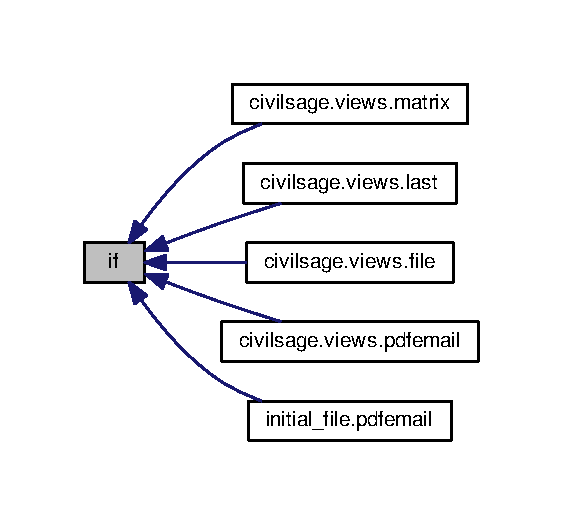
\includegraphics[width=350pt]{bootstrap_8min_8js_ac2d69f5011896c6ed4a54e0dd36f6334_icgraph}
\end{center}
\end{figure}


\hypertarget{bootstrap_8min_8js_a87cf461060832b8b68a7b48d9e371e4f}{}\index{bootstrap.\+min.\+js@{bootstrap.\+min.\+js}!if@{if}}
\index{if@{if}!bootstrap.\+min.\+js@{bootstrap.\+min.\+js}}
\subsubsection[{if(b[0]$<$ 2 \&\&b[1]$<$ 9\texttt{"|}\texttt{"|}1==b[0]\&\&9==b[1]\&\&b[2]$<$ 1) throw new Error(""Bootstrap\textquotesingle{}s Java\+Script requires j\+Query version 1.\+9.\+1 or higher"")\rcurly{}(j\+Query)}]{\setlength{\rightskip}{0pt plus 5cm}if (
\begin{DoxyParamCaption}
{}
\end{DoxyParamCaption}
)\hspace{0.3cm}{\ttfamily [new]}}\label{bootstrap_8min_8js_a87cf461060832b8b68a7b48d9e371e4f}


\subsection{Variable Documentation}
\hypertarget{bootstrap_8min_8js_ae8f6b400ed3390908c5cdeebed3a82b9}{}\index{bootstrap.\+min.\+js@{bootstrap.\+min.\+js}!a@{a}}
\index{a@{a}!bootstrap.\+min.\+js@{bootstrap.\+min.\+js}}
\subsubsection[{a}]{\setlength{\rightskip}{0pt plus 5cm}a {\bf fn} a {\bf fn} {\bf button} a {\bf fn} {\bf button} a \{\char`\"{}use strict\char`\"{}}\label{bootstrap_8min_8js_ae8f6b400ed3390908c5cdeebed3a82b9}


Definition at line \hyperlink{bootstrap_8min_8js_source_l00006}{6} of file \hyperlink{bootstrap_8min_8js_source}{bootstrap.\+min.\+js}.

\hypertarget{bootstrap_8min_8js_aaa41eef066735d697e7786ec86d52389}{}\index{bootstrap.\+min.\+js@{bootstrap.\+min.\+js}!alert@{alert}}
\index{alert@{alert}!bootstrap.\+min.\+js@{bootstrap.\+min.\+js}}
\subsubsection[{alert}]{\setlength{\rightskip}{0pt plus 5cm}{\bf a} {\bf fn} alert ={\bf b}}\label{bootstrap_8min_8js_aaa41eef066735d697e7786ec86d52389}


Definition at line \hyperlink{bootstrap_8min_8js_source_l00006}{6} of file \hyperlink{bootstrap_8min_8js_source}{bootstrap.\+min.\+js}.

\hypertarget{bootstrap_8min_8js_ac0431efac4d7c393d1e70b86115cb93f}{}\index{bootstrap.\+min.\+js@{bootstrap.\+min.\+js}!b@{b}}
\index{b@{b}!bootstrap.\+min.\+js@{bootstrap.\+min.\+js}}
\subsubsection[{b}]{\setlength{\rightskip}{0pt plus 5cm}function b =a.\+fn.\+jquery.\+split(\char`\"{} \char`\"{})\mbox{[}0\mbox{]}.split(\char`\"{}.\char`\"{})}\label{bootstrap_8min_8js_ac0431efac4d7c393d1e70b86115cb93f}


Definition at line \hyperlink{bootstrap_8min_8js_source_l00006}{6} of file \hyperlink{bootstrap_8min_8js_source}{bootstrap.\+min.\+js}.

\hypertarget{bootstrap_8min_8js_a55e170814e74f6c3db8ae9ea3ba9054f}{}\index{bootstrap.\+min.\+js@{bootstrap.\+min.\+js}!button@{button}}
\index{button@{button}!bootstrap.\+min.\+js@{bootstrap.\+min.\+js}}
\subsubsection[{button}]{\setlength{\rightskip}{0pt plus 5cm}{\bf a} {\bf fn} button ={\bf b}}\label{bootstrap_8min_8js_a55e170814e74f6c3db8ae9ea3ba9054f}


Definition at line \hyperlink{bootstrap_8min_8js_source_l00006}{6} of file \hyperlink{bootstrap_8min_8js_source}{bootstrap.\+min.\+js}.

\hypertarget{bootstrap_8min_8js_ad9d1ac02e33c4aed62ad517a7cb8b3fb}{}\index{bootstrap.\+min.\+js@{bootstrap.\+min.\+js}!c@{c}}
\index{c@{c}!bootstrap.\+min.\+js@{bootstrap.\+min.\+js}}
\subsubsection[{c}]{\setlength{\rightskip}{0pt plus 5cm}function c =\textquotesingle{}\mbox{[}data-\/dismiss=\char`\"{}alert\char`\"{}\mbox{]}\textquotesingle{}}\label{bootstrap_8min_8js_ad9d1ac02e33c4aed62ad517a7cb8b3fb}


Definition at line \hyperlink{bootstrap_8min_8js_source_l00006}{6} of file \hyperlink{bootstrap_8min_8js_source}{bootstrap.\+min.\+js}.

\hypertarget{bootstrap_8min_8js_a72fbb3628c3cc943ced8aad64247888c}{}\index{bootstrap.\+min.\+js@{bootstrap.\+min.\+js}!close@{close}}
\index{close@{close}!bootstrap.\+min.\+js@{bootstrap.\+min.\+js}}
\subsubsection[{close}]{\setlength{\rightskip}{0pt plus 5cm}{\bf d} {\bf d} {\bf d} prototype close =function({\bf b})\{function {\bf c}()\{g.\+detach().trigger(\char`\"{}closed.\+bs.\+alert\char`\"{}).remove()\}var {\bf e}={\bf a}(this),f=e.\+attr(\char`\"{}data-\/target\char`\"{});f$\vert$$\vert$(f=e.\+attr(\char`\"{}href\char`\"{}),f=f\&\&f.\+replace(/.$\ast$(?=\#\mbox{[}$^\wedge$\textbackslash{}s\mbox{]}$\ast$\$)/,\char`\"{}\char`\"{}));var g={\bf a}(f);{\bf b}\&\&b.\+prevent\+Default(),g.\+length$\vert$$\vert$(g=e.\+closest(\char`\"{}.alert\char`\"{})),g.\+trigger({\bf b}=a.\+Event(\char`\"{}close.\+bs.\+alert\char`\"{})),b.\+is\+Default\+Prevented()$\vert$$\vert$(g.\+remove\+Class(\char`\"{}in\char`\"{}),a.\+support.\+transition\&\&{\bf g.\+has\+Class}(\char`\"{}fade\char`\"{})?g.\+one(\char`\"{}bs\+Transition\+End\char`\"{},c).{\bf emulate\+Transition\+End}({\bf d.\+T\+R\+A\+N\+S\+I\+T\+I\+O\+N\+\_\+\+D\+U\+R\+A\+T\+I\+O\+N})\+:{\bf c}())\}}\label{bootstrap_8min_8js_a72fbb3628c3cc943ced8aad64247888c}


Definition at line \hyperlink{bootstrap_8min_8js_source_l00006}{6} of file \hyperlink{bootstrap_8min_8js_source}{bootstrap.\+min.\+js}.

\hypertarget{bootstrap_8min_8js_a0545907c609a48549a0cf5d4c692f851}{}\index{bootstrap.\+min.\+js@{bootstrap.\+min.\+js}!Constructor@{Constructor}}
\index{Constructor@{Constructor}!bootstrap.\+min.\+js@{bootstrap.\+min.\+js}}
\subsubsection[{Constructor}]{\setlength{\rightskip}{0pt plus 5cm}{\bf a} {\bf fn} {\bf a} {\bf fn} {\bf button} Constructor ={\bf d}}\label{bootstrap_8min_8js_a0545907c609a48549a0cf5d4c692f851}


Definition at line \hyperlink{bootstrap_8min_8js_source_l00006}{6} of file \hyperlink{bootstrap_8min_8js_source}{bootstrap.\+min.\+js}.

\hypertarget{bootstrap_8min_8js_aeb337d295abaddb5ec3cb34cc2e2bbc9}{}\index{bootstrap.\+min.\+js@{bootstrap.\+min.\+js}!d@{d}}
\index{d@{d}!bootstrap.\+min.\+js@{bootstrap.\+min.\+js}}
\subsubsection[{d}]{\setlength{\rightskip}{0pt plus 5cm}var d =function({\bf b})\{{\bf a}({\bf b}).on(\char`\"{}click\char`\"{},c,{\bf this.\+close})\}}\label{bootstrap_8min_8js_aeb337d295abaddb5ec3cb34cc2e2bbc9}


Definition at line \hyperlink{bootstrap_8min_8js_source_l00006}{6} of file \hyperlink{bootstrap_8min_8js_source}{bootstrap.\+min.\+js}.

\hypertarget{bootstrap_8min_8js_a6c1cf0be5e5383617ddc5efdfdc8c651}{}\index{bootstrap.\+min.\+js@{bootstrap.\+min.\+js}!D\+E\+F\+A\+U\+L\+T\+S@{D\+E\+F\+A\+U\+L\+T\+S}}
\index{D\+E\+F\+A\+U\+L\+T\+S@{D\+E\+F\+A\+U\+L\+T\+S}!bootstrap.\+min.\+js@{bootstrap.\+min.\+js}}
\subsubsection[{D\+E\+F\+A\+U\+L\+T\+S}]{\setlength{\rightskip}{0pt plus 5cm}{\bf c} {\bf c} D\+E\+F\+A\+U\+L\+T\+S =\{loading\+Text\+:\char`\"{}loading...\char`\"{}\}}\label{bootstrap_8min_8js_a6c1cf0be5e5383617ddc5efdfdc8c651}


Definition at line \hyperlink{bootstrap_8min_8js_source_l00006}{6} of file \hyperlink{bootstrap_8min_8js_source}{bootstrap.\+min.\+js}.

\hypertarget{bootstrap_8min_8js_ab5902775854a8b8440bcd25e0fe1c120}{}\index{bootstrap.\+min.\+js@{bootstrap.\+min.\+js}!e@{e}}
\index{e@{e}!bootstrap.\+min.\+js@{bootstrap.\+min.\+js}}
\subsubsection[{e}]{\setlength{\rightskip}{0pt plus 5cm}var e ={\bf a.\+fn.\+alert}}\label{bootstrap_8min_8js_ab5902775854a8b8440bcd25e0fe1c120}


Definition at line \hyperlink{bootstrap_8min_8js_source_l00006}{6} of file \hyperlink{bootstrap_8min_8js_source}{bootstrap.\+min.\+js}.

\hypertarget{bootstrap_8min_8js_a006fe6a2a254572b367123c6db401ff3}{}\index{bootstrap.\+min.\+js@{bootstrap.\+min.\+js}!emulate\+Transition\+End@{emulate\+Transition\+End}}
\index{emulate\+Transition\+End@{emulate\+Transition\+End}!bootstrap.\+min.\+js@{bootstrap.\+min.\+js}}
\subsubsection[{emulate\+Transition\+End}]{\setlength{\rightskip}{0pt plus 5cm}{\bf a} {\bf fn} emulate\+Transition\+End =function({\bf b})\{var {\bf c}=!1,{\bf d}=this;{\bf a}(this).one(\char`\"{}bs\+Transition\+End\char`\"{},function()\{{\bf c}=!0\});var {\bf e}=function()\{{\bf c}$\vert$$\vert${\bf a}({\bf d}).trigger(a.\+support.\+transition.\+end)\};return set\+Timeout({\bf e},{\bf b}),this\}}\label{bootstrap_8min_8js_a006fe6a2a254572b367123c6db401ff3}


Definition at line \hyperlink{bootstrap_8min_8js_source_l00006}{6} of file \hyperlink{bootstrap_8min_8js_source}{bootstrap.\+min.\+js}.

\hypertarget{bootstrap_8min_8js_ac26971afe341e4079ee34fceab395fc2}{}\index{bootstrap.\+min.\+js@{bootstrap.\+min.\+js}!no\+Conflict@{no\+Conflict}}
\index{no\+Conflict@{no\+Conflict}!bootstrap.\+min.\+js@{bootstrap.\+min.\+js}}
\subsubsection[{no\+Conflict}]{\setlength{\rightskip}{0pt plus 5cm}{\bf a} {\bf fn} {\bf a} {\bf fn} {\bf button} {\bf a} {\bf fn} {\bf button} no\+Conflict =function()\{return {\bf a.\+fn.\+alert}={\bf e},this\}}\label{bootstrap_8min_8js_ac26971afe341e4079ee34fceab395fc2}


Definition at line \hyperlink{bootstrap_8min_8js_source_l00006}{6} of file \hyperlink{bootstrap_8min_8js_source}{bootstrap.\+min.\+js}.

\hypertarget{bootstrap_8min_8js_a14f119ea3b5abc5536d590dfe1793c6e}{}\index{bootstrap.\+min.\+js@{bootstrap.\+min.\+js}!set\+State@{set\+State}}
\index{set\+State@{set\+State}!bootstrap.\+min.\+js@{bootstrap.\+min.\+js}}
\subsubsection[{set\+State}]{\setlength{\rightskip}{0pt plus 5cm}{\bf c} {\bf c} {\bf c} prototype set\+State =function({\bf b})\{var {\bf c}=\char`\"{}disabled\char`\"{},d=this.\$element,{\bf e}=d.\+is(\char`\"{}input\char`\"{})?\char`\"{}val\char`\"{}\+:\char`\"{}html\char`\"{},f=d.\+data();{\bf b}+=\char`\"{}Text\char`\"{},null==f.\+reset\+Text\&\&d.\+data(\char`\"{}reset\+Text\char`\"{},d\mbox{[}{\bf e}\mbox{]}()),set\+Timeout(a.\+proxy(function()\{{\bf d}\mbox{[}{\bf e}\mbox{]}(null==f\mbox{[}{\bf b}\mbox{]}?this.\+options\mbox{[}{\bf b}\mbox{]}\+:f\mbox{[}{\bf b}\mbox{]}),\char`\"{}loading\+Text\char`\"{}==b?(this.\+is\+Loading=!0,d.\+add\+Class({\bf c}).attr({\bf c},{\bf c}))\+:this.\+is\+Loading\&\&(this.\+is\+Loading=!1,d.\+remove\+Class({\bf c}).remove\+Attr({\bf c}))\},this),0)\}}\label{bootstrap_8min_8js_a14f119ea3b5abc5536d590dfe1793c6e}


Definition at line \hyperlink{bootstrap_8min_8js_source_l00006}{6} of file \hyperlink{bootstrap_8min_8js_source}{bootstrap.\+min.\+js}.

\hypertarget{bootstrap_8min_8js_aa8e797a9bda5e7e313be3518054164a3}{}\index{bootstrap.\+min.\+js@{bootstrap.\+min.\+js}!toggle@{toggle}}
\index{toggle@{toggle}!bootstrap.\+min.\+js@{bootstrap.\+min.\+js}}
\subsubsection[{toggle}]{\setlength{\rightskip}{0pt plus 5cm}{\bf c} {\bf c} {\bf c} prototype {\bf c} prototype toggle =function()\{var {\bf a}=!0,{\bf b}=this.\$element.\+closest(\textquotesingle{}\mbox{[}data-\/toggle=\char`\"{}buttons\char`\"{}\mbox{]}\textquotesingle{});if(b.\+length)\{var {\bf c}=this.\$element.\+find(\char`\"{}input\char`\"{});\char`\"{}radio\char`\"{}==c.\+prop(\char`\"{}type\char`\"{})?(c.\+prop(\char`\"{}checked\char`\"{})\&\&(a=!1),b.\+find(\char`\"{}.active\char`\"{}).remove\+Class(\char`\"{}active\char`\"{}),this.\$element.\+add\+Class(\char`\"{}active\char`\"{}))\+:\char`\"{}checkbox\char`\"{}==c.\+prop(\char`\"{}type\char`\"{})\&\&(c.\+prop(\char`\"{}checked\char`\"{})!==this.\$element.\+has\+Class(\char`\"{}active\char`\"{})\&\&(a=!1),this.\$element.\+toggle\+Class(\char`\"{}active\char`\"{})),c.\+prop(\char`\"{}checked\char`\"{},this.\$element.\+has\+Class(\char`\"{}active\char`\"{})),a\&\&c.\+trigger(\char`\"{}change\char`\"{})\}else this.\$element.\+attr(\char`\"{}aria-\/pressed\char`\"{},!this.\$element.\+has\+Class(\char`\"{}active\char`\"{})),this.\$element.\+toggle\+Class(\char`\"{}active\char`\"{})\}}\label{bootstrap_8min_8js_aa8e797a9bda5e7e313be3518054164a3}


Definition at line \hyperlink{bootstrap_8min_8js_source_l00006}{6} of file \hyperlink{bootstrap_8min_8js_source}{bootstrap.\+min.\+js}.

\hypertarget{bootstrap_8min_8js_ae4adb159aeacba734c34bd530baf92f6}{}\index{bootstrap.\+min.\+js@{bootstrap.\+min.\+js}!T\+R\+A\+N\+S\+I\+T\+I\+O\+N\+\_\+\+D\+U\+R\+A\+T\+I\+O\+N@{T\+R\+A\+N\+S\+I\+T\+I\+O\+N\+\_\+\+D\+U\+R\+A\+T\+I\+O\+N}}
\index{T\+R\+A\+N\+S\+I\+T\+I\+O\+N\+\_\+\+D\+U\+R\+A\+T\+I\+O\+N@{T\+R\+A\+N\+S\+I\+T\+I\+O\+N\+\_\+\+D\+U\+R\+A\+T\+I\+O\+N}!bootstrap.\+min.\+js@{bootstrap.\+min.\+js}}
\subsubsection[{T\+R\+A\+N\+S\+I\+T\+I\+O\+N\+\_\+\+D\+U\+R\+A\+T\+I\+O\+N}]{\setlength{\rightskip}{0pt plus 5cm}{\bf d} {\bf d} T\+R\+A\+N\+S\+I\+T\+I\+O\+N\+\_\+\+D\+U\+R\+A\+T\+I\+O\+N =150}\label{bootstrap_8min_8js_ae4adb159aeacba734c34bd530baf92f6}


Definition at line \hyperlink{bootstrap_8min_8js_source_l00006}{6} of file \hyperlink{bootstrap_8min_8js_source}{bootstrap.\+min.\+js}.

\hypertarget{bootstrap_8min_8js_a3635f2df5844f69204b70bf7b3983587}{}\index{bootstrap.\+min.\+js@{bootstrap.\+min.\+js}!V\+E\+R\+S\+I\+O\+N@{V\+E\+R\+S\+I\+O\+N}}
\index{V\+E\+R\+S\+I\+O\+N@{V\+E\+R\+S\+I\+O\+N}!bootstrap.\+min.\+js@{bootstrap.\+min.\+js}}
\subsubsection[{V\+E\+R\+S\+I\+O\+N}]{\setlength{\rightskip}{0pt plus 5cm}{\bf c} V\+E\+R\+S\+I\+O\+N =\char`\"{}3.\+3.\+5\char`\"{}}\label{bootstrap_8min_8js_a3635f2df5844f69204b70bf7b3983587}


Definition at line \hyperlink{bootstrap_8min_8js_source_l00006}{6} of file \hyperlink{bootstrap_8min_8js_source}{bootstrap.\+min.\+js}.


\hypertarget{bootstrap_8min_8js_source}{}\section{bootstrap.\+min.\+js}
\label{bootstrap_8min_8js_source}\index{/home/amarjeet/projects/\+Civil\+Octave/sage/static/js/bootstrap.\+min.\+js@{/home/amarjeet/projects/\+Civil\+Octave/sage/static/js/bootstrap.\+min.\+js}}

\begin{DoxyCode}
00001 
\hypertarget{bootstrap_8min_8js_source_l00006}{}\hyperlink{bootstrap_8min_8js_a3635f2df5844f69204b70bf7b3983587}{00006} \textcolor{keywordflow}{if}(\textcolor{stringliteral}{"undefined"}==typeof jQuery)\textcolor{keywordflow}{throw} \textcolor{keyword}{new} Error(\textcolor{stringliteral}{"Bootstrap's JavaScript requires jQuery"});+\textcolor{keyword}{function}(
      \hyperlink{bootstrap_8min_8js_ae8f6b400ed3390908c5cdeebed3a82b9}{a})\{\textcolor{stringliteral}{"use strict"};var \hyperlink{bootstrap_8min_8js_ac0431efac4d7c393d1e70b86115cb93f}{b}=\hyperlink{bootstrap_8min_8js_ae8f6b400ed3390908c5cdeebed3a82b9}{a}.fn.jquery.split(\textcolor{stringliteral}{" "})[0].split(\textcolor{stringliteral}{"."});\textcolor{keywordflow}{if}(b[0]<2&&b[1]<9||1==b[0]&&9==b[1]&&b[2]<1)\textcolor{keywordflow}{
      throw} \textcolor{keyword}{new} Error(\textcolor{stringliteral}{"Bootstrap's JavaScript requires jQuery version 1.9.1 or higher"})\}(jQuery),+\textcolor{keyword}{function}(
      \hyperlink{bootstrap_8min_8js_ae8f6b400ed3390908c5cdeebed3a82b9}{a})\{\textcolor{stringliteral}{"use strict"};\textcolor{keyword}{function} \hyperlink{bootstrap_8min_8js_ac0431efac4d7c393d1e70b86115cb93f}{b}()\{var \hyperlink{bootstrap_8min_8js_ae8f6b400ed3390908c5cdeebed3a82b9}{a}=document.createElement(\textcolor{stringliteral}{"bootstrap"}),b=\{WebkitTransition:\textcolor{stringliteral}{"
      webkitTransitionEnd"},MozTransition:\textcolor{stringliteral}{"transitionend"},OTransition:\textcolor{stringliteral}{"oTransitionEnd otransitionend"},transition:\textcolor{stringliteral}{"transitionend
      "}\};\textcolor{keywordflow}{for}(var \hyperlink{bootstrap_8min_8js_ad9d1ac02e33c4aed62ad517a7cb8b3fb}{c} in b)\textcolor{keywordflow}{if}(\textcolor{keywordtype}{void} 0!==a.style[\hyperlink{bootstrap_8min_8js_ad9d1ac02e33c4aed62ad517a7cb8b3fb}{c}])\textcolor{keywordflow}{return}\{end:b[\hyperlink{bootstrap_8min_8js_ad9d1ac02e33c4aed62ad517a7cb8b3fb}{c}]\};\textcolor{keywordflow}{return}!1\}a.fn.emulateTransitionEnd=\textcolor{keyword}{function}(
      \hyperlink{bootstrap_8min_8js_ac0431efac4d7c393d1e70b86115cb93f}{b})\{var \hyperlink{bootstrap_8min_8js_ad9d1ac02e33c4aed62ad517a7cb8b3fb}{c}=!1,\hyperlink{bootstrap_8min_8js_aeb337d295abaddb5ec3cb34cc2e2bbc9}{d}=\textcolor{keyword}{this};\hyperlink{bootstrap_8min_8js_ae8f6b400ed3390908c5cdeebed3a82b9}{a}(\textcolor{keyword}{this}).one(\textcolor{stringliteral}{"bsTransitionEnd"},\textcolor{keyword}{function}()\{c=!0\});var \hyperlink{bootstrap_8min_8js_ab5902775854a8b8440bcd25e0fe1c120}{e}=\textcolor{keyword}{function}()\{c||
      \hyperlink{bootstrap_8min_8js_ae8f6b400ed3390908c5cdeebed3a82b9}{a}(\hyperlink{bootstrap_8min_8js_aeb337d295abaddb5ec3cb34cc2e2bbc9}{d}).trigger(a.support.transition.end)\};\textcolor{keywordflow}{return} setTimeout(e,b),\textcolor{keyword}{this}\},\hyperlink{bootstrap_8min_8js_ae8f6b400ed3390908c5cdeebed3a82b9}{a}(\textcolor{keyword}{function}()\{a.support.transition=
      \hyperlink{bootstrap_8min_8js_ac0431efac4d7c393d1e70b86115cb93f}{b}(),a.support.transition&&(a.event.special.bsTransitionEnd=\{bindType:a.support.transition.end,delegateType
      :a.support.transition.end,handle:\textcolor{keyword}{function}(\hyperlink{bootstrap_8min_8js_ac0431efac4d7c393d1e70b86115cb93f}{b})\{\textcolor{keywordflow}{return} \hyperlink{bootstrap_8min_8js_ae8f6b400ed3390908c5cdeebed3a82b9}{a}(b.target).is(\textcolor{keyword}{this})?b.handleObj.handler.apply(\textcolor{keyword}{this},
      arguments):\textcolor{keywordtype}{void} 0\}\})\})\}(jQuery),+\textcolor{keyword}{function}(a)\{\textcolor{stringliteral}{"use strict"};\textcolor{keyword}{function} \hyperlink{bootstrap_8min_8js_ac0431efac4d7c393d1e70b86115cb93f}{b}(b)\{\textcolor{keywordflow}{return} this.
      \hyperlink{jquery_8min_8js_a18d9b499a0765bf2fe5f372ff2fc0236}{each}(\textcolor{keyword}{function}()\{var c=\hyperlink{bootstrap_8min_8js_ae8f6b400ed3390908c5cdeebed3a82b9}{a}(\textcolor{keyword}{this}),e=c.data(\textcolor{stringliteral}{"bs.alert"});e||c.data(\textcolor{stringliteral}{"bs.alert"},e=\textcolor{keyword}{new} 
      \hyperlink{bootstrap_8min_8js_aeb337d295abaddb5ec3cb34cc2e2bbc9}{d}(\textcolor{keyword}{this})),\textcolor{stringliteral}{"string"}==typeof b&&e[\hyperlink{bootstrap_8min_8js_ac0431efac4d7c393d1e70b86115cb93f}{b}].call(c)\})\}var c=\textcolor{stringliteral}{'[data-dismiss="alert"]'},\hyperlink{bootstrap_8min_8js_aeb337d295abaddb5ec3cb34cc2e2bbc9}{d}=\textcolor{keyword}{function}(b)\{
      \hyperlink{bootstrap_8min_8js_ae8f6b400ed3390908c5cdeebed3a82b9}{a}(b).on(\textcolor{stringliteral}{"click"},c,this.\hyperlink{bootstrap_8min_8js_a72fbb3628c3cc943ced8aad64247888c}{close})\};\hyperlink{bootstrap_8min_8js_aeb337d295abaddb5ec3cb34cc2e2bbc9}{d}.VERSION=\textcolor{stringliteral}{"3.3.5"},\hyperlink{bootstrap_8min_8js_aeb337d295abaddb5ec3cb34cc2e2bbc9}{d}.TRANSITION\_DURATION=150,
      \hyperlink{bootstrap_8min_8js_aeb337d295abaddb5ec3cb34cc2e2bbc9}{d}.prototype.close=\textcolor{keyword}{function}(\hyperlink{bootstrap_8min_8js_ac0431efac4d7c393d1e70b86115cb93f}{b})\{\textcolor{keyword}{function} \hyperlink{bootstrap_8min_8js_ad9d1ac02e33c4aed62ad517a7cb8b3fb}{c}()\{g.detach().trigger(\textcolor{stringliteral}{"closed.bs.alert"}).remove()\}var e=
      \hyperlink{bootstrap_8min_8js_ae8f6b400ed3390908c5cdeebed3a82b9}{a}(\textcolor{keyword}{this}),f=e.attr(\textcolor{stringliteral}{"data-target"});f||(f=e.attr(\textcolor{stringliteral}{"href"}),f=f&&f.replace(/.*(?=#[^\(\backslash\)s]*$)/,\textcolor{stringliteral}{""}));var g=
      \hyperlink{bootstrap_8min_8js_ae8f6b400ed3390908c5cdeebed3a82b9}{a}(f);b&&b.preventDefault(),g.length||(g=e.closest(\textcolor{stringliteral}{".alert"})),g.trigger(b=a.Event(\textcolor{stringliteral}{"close.bs.alert"})),b.
      isDefaultPrevented()||(g.removeClass(\textcolor{stringliteral}{"in"}),a.support.transition&&g.hasClass(\textcolor{stringliteral}{"fade"})?g.one(\textcolor{stringliteral}{"bsTransitionEnd"},c).
      emulateTransitionEnd(\hyperlink{bootstrap_8min_8js_aeb337d295abaddb5ec3cb34cc2e2bbc9}{d}.TRANSITION\_DURATION):\hyperlink{bootstrap_8min_8js_ad9d1ac02e33c4aed62ad517a7cb8b3fb}{c}())\};var e=a.fn.alert;a.fn.alert=\hyperlink{bootstrap_8min_8js_ac0431efac4d7c393d1e70b86115cb93f}{b},a.fn.alert.Constructor=
      \hyperlink{bootstrap_8min_8js_aeb337d295abaddb5ec3cb34cc2e2bbc9}{d},a.fn.alert.noConflict=\textcolor{keyword}{function}()\{\textcolor{keywordflow}{return} a.fn.alert=\hyperlink{bootstrap_8min_8js_ab5902775854a8b8440bcd25e0fe1c120}{e},\textcolor{keyword}{this}\},\hyperlink{bootstrap_8min_8js_ae8f6b400ed3390908c5cdeebed3a82b9}{a}(document).on(\textcolor{stringliteral}{"click.bs.alert.data-api"},c,
      \hyperlink{bootstrap_8min_8js_aeb337d295abaddb5ec3cb34cc2e2bbc9}{d}.prototype.close)\}(jQuery),+\textcolor{keyword}{function}(a)\{\textcolor{stringliteral}{"use strict"};\textcolor{keyword}{function} \hyperlink{bootstrap_8min_8js_ac0431efac4d7c393d1e70b86115cb93f}{b}(b)\{\textcolor{keywordflow}{return} this.
      \hyperlink{jquery_8min_8js_a18d9b499a0765bf2fe5f372ff2fc0236}{each}(\textcolor{keyword}{function}()\{var \hyperlink{bootstrap_8min_8js_aeb337d295abaddb5ec3cb34cc2e2bbc9}{d}=\hyperlink{bootstrap_8min_8js_ae8f6b400ed3390908c5cdeebed3a82b9}{a}(\textcolor{keyword}{this}),e=d.data(\textcolor{stringliteral}{"bs.button"}),f=\textcolor{stringliteral}{"object"}==typeof b&&
      \hyperlink{bootstrap_8min_8js_ac0431efac4d7c393d1e70b86115cb93f}{b};e||d.data(\textcolor{stringliteral}{"bs.button"},e=\textcolor{keyword}{new} \hyperlink{bootstrap_8min_8js_ad9d1ac02e33c4aed62ad517a7cb8b3fb}{c}(\textcolor{keyword}{this},f)),\textcolor{stringliteral}{"toggle"}==b?e.toggle():b&&e.setState(b)\})\}var c=\textcolor{keyword}{function}(b,d)\{
      this.$element=\hyperlink{bootstrap_8min_8js_ae8f6b400ed3390908c5cdeebed3a82b9}{a}(b),this.options=a.extend(\{\},c.DEFAULTS,\hyperlink{bootstrap_8min_8js_aeb337d295abaddb5ec3cb34cc2e2bbc9}{d}),this.isLoading=!1\};c.VERSION=\textcolor{stringliteral}{"3.3.5"},c.DEFAULTS=\{
      loadingText:\textcolor{stringliteral}{"loading..."}\},c.prototype.setState=\textcolor{keyword}{function}(\hyperlink{bootstrap_8min_8js_ac0431efac4d7c393d1e70b86115cb93f}{b})\{var c=\textcolor{stringliteral}{"disabled"},d=this.$element,e=d.is(\textcolor{stringliteral}{"input"})?\textcolor{stringliteral}{
      "val"}:\textcolor{stringliteral}{"html"},f=d.data();b+=\textcolor{stringliteral}{"Text"},null==f.resetText&&d.data(\textcolor{stringliteral}{"resetText"},d[e]()),setTimeout(a.proxy(\textcolor{keyword}{function}(
      )\{d[e](null==f[b]?this.options[b]:f[b]),\textcolor{stringliteral}{"loadingText"}==b?(this.isLoading=!0,d.addClass(c).attr(c,c)):this.is
      Loading&&(this.isLoading=!1,d.removeClass(c).removeAttr(c))\},\textcolor{keyword}{this}),0)\},c.prototype.toggle=\textcolor{keyword}{function}()\{var a=!
      0,b=this.$element.closest(\textcolor{stringliteral}{'[data-toggle="buttons"]'});\textcolor{keywordflow}{if}(b.length)\{var c=this.$element.find(\textcolor{stringliteral}{"input"});\textcolor{stringliteral}{"radio"}=
      =c.prop(\textcolor{stringliteral}{"type"})?(c.prop(\textcolor{stringliteral}{"checked"})&&(a=!1),b.find(\textcolor{stringliteral}{".active"}).removeClass(\textcolor{stringliteral}{"active"}),this.$element.addClass(\textcolor{stringliteral}{"
      active"})):\textcolor{stringliteral}{"checkbox"}==c.prop(\textcolor{stringliteral}{"type"})&&(c.prop(\textcolor{stringliteral}{"checked"})!==this.$element.hasClass(\textcolor{stringliteral}{"active"})&&(a=!1),this.
      $element.toggleClass(\textcolor{stringliteral}{"active"})),c.prop(\textcolor{stringliteral}{"checked"},\textcolor{keyword}{this}.$element.hasClass(\textcolor{stringliteral}{"active"})),a&&c.trigger(\textcolor{stringliteral}{"change"})\}\textcolor{keywordflow}{else} 
      this.$element.attr(\textcolor{stringliteral}{"aria-pressed"},!this.$element.hasClass(\textcolor{stringliteral}{"active"})),this.$element.toggleClass(\textcolor{stringliteral}{"active"})\};var
       d=a.fn.button;a.fn.button=\hyperlink{bootstrap_8min_8js_ac0431efac4d7c393d1e70b86115cb93f}{b},a.fn.button.Constructor=\hyperlink{bootstrap_8min_8js_ad9d1ac02e33c4aed62ad517a7cb8b3fb}{c},a.fn.button.noConflict=\textcolor{keyword}{function}()\{\textcolor{keywordflow}{return} a.fn.
      button=\hyperlink{bootstrap_8min_8js_aeb337d295abaddb5ec3cb34cc2e2bbc9}{d},\textcolor{keyword}{this}\},\hyperlink{bootstrap_8min_8js_ae8f6b400ed3390908c5cdeebed3a82b9}{a}(document).on(\textcolor{stringliteral}{"click.bs.button.data-api"},\textcolor{stringliteral}{'[data-toggle^="button"]'},\textcolor{keyword}{function}(c)\{var d=
      \hyperlink{bootstrap_8min_8js_ae8f6b400ed3390908c5cdeebed3a82b9}{a}(c.target);d.hasClass(\textcolor{stringliteral}{"btn"})||(d=d.closest(\textcolor{stringliteral}{".btn"})),b.call(d,\textcolor{stringliteral}{"toggle"}),\hyperlink{bootstrap_8min_8js_ae8f6b400ed3390908c5cdeebed3a82b9}{a}(c.target).is(\textcolor{stringliteral}{'
      input[type="radio"]'})||\hyperlink{bootstrap_8min_8js_ae8f6b400ed3390908c5cdeebed3a82b9}{a}(c.target).is(\textcolor{stringliteral}{'input[type="checkbox"]'})||c.preventDefault()\}).on(\textcolor{stringliteral}{"focus.bs.button.data-api
       blur.bs.button.data-api"},\textcolor{stringliteral}{'[data-toggle^="button"]'},\textcolor{keyword}{function}(b)\{\hyperlink{bootstrap_8min_8js_ae8f6b400ed3390908c5cdeebed3a82b9}{a}(b.target).closest(\textcolor{stringliteral}{".btn"}).toggleClass(\textcolor{stringliteral}{"focus"},/^
      focus(in)?$/.test(b.type))\})\}(jQuery),+\textcolor{keyword}{function}(\hyperlink{bootstrap_8min_8js_ae8f6b400ed3390908c5cdeebed3a82b9}{a})\{\textcolor{stringliteral}{"use strict"};\textcolor{keyword}{function} \hyperlink{bootstrap_8min_8js_ac0431efac4d7c393d1e70b86115cb93f}{b}(b)\{\textcolor{keywordflow}{return} this.
      \hyperlink{jquery_8min_8js_a18d9b499a0765bf2fe5f372ff2fc0236}{each}(\textcolor{keyword}{function}()\{var d=\hyperlink{bootstrap_8min_8js_ae8f6b400ed3390908c5cdeebed3a82b9}{a}(\textcolor{keyword}{this}),e=d.data(\textcolor{stringliteral}{"bs.carousel"}),f=a.extend(\{\},c.DEFAULTS,d.data(),\textcolor{stringliteral}{"object"}==
      typeof b&&\hyperlink{bootstrap_8min_8js_ac0431efac4d7c393d1e70b86115cb93f}{b}),g=\textcolor{stringliteral}{"string"}==typeof b?b:f.slide;e||d.data(\textcolor{stringliteral}{"bs.carousel"},e=\textcolor{keyword}{new} c(\textcolor{keyword}{this},f)),\textcolor{stringliteral}{"number"}==typeof b?e.to(b)
      :g?e[g]():f.interval&&e.pause().cycle()\})\}var c=\textcolor{keyword}{function}(b,c)\{this.$element=\hyperlink{bootstrap_8min_8js_ae8f6b400ed3390908c5cdeebed3a82b9}{a}(b),this.$indicators=this.
      $element.find(\textcolor{stringliteral}{".carousel-indicators"}),this.options=\hyperlink{bootstrap_8min_8js_ad9d1ac02e33c4aed62ad517a7cb8b3fb}{c},this.paused=null,this.sliding=null,this.interval=null,
      this.$active=null,this.$items=null,this.options.keyboard&&this.$element.on(\textcolor{stringliteral}{"keydown.bs.carousel"},a.proxy(\textcolor{keyword}{this}.
      keydown,\textcolor{keyword}{this})),\textcolor{stringliteral}{"hover"}==this.options.pause&&!(\textcolor{stringliteral}{"ontouchstart"}in document.documentElement)&&this.$element.on(\textcolor{stringliteral}{"
      mouseenter.bs.carousel"},a.proxy(\textcolor{keyword}{this}.pause,\textcolor{keyword}{this})).on(\textcolor{stringliteral}{"mouseleave.bs.carousel"},a.proxy(\textcolor{keyword}{this}.cycle,\textcolor{keyword}{this}))\};c.
      VERSION=\textcolor{stringliteral}{"3.3.5"},c.TRANSITION\_DURATION=600,c.DEFAULTS=\{interval:5e3,pause:\textcolor{stringliteral}{"hover"},wrap:!0,keyboard:!0\},c.
      prototype.keydown=\textcolor{keyword}{function}(\hyperlink{bootstrap_8min_8js_ae8f6b400ed3390908c5cdeebed3a82b9}{a})\{\textcolor{keywordflow}{if}(!/\hyperlink{namespaceinput}{input}|textarea/\hyperlink{DoS_201_2main_8m_a6dbbc96f4222af2f6c18c8e60f41726b}{i}.test(a.target.tagName))\{\textcolor{keywordflow}{switch}(a.which)\{\textcolor{keywordflow}{case} 37:this.
      prev();\textcolor{keywordflow}{break};\textcolor{keywordflow}{case} 39:this.next();\textcolor{keywordflow}{break};\textcolor{keywordflow}{default}:\textcolor{keywordflow}{return}\}a.preventDefault()\}\},c.prototype.cycle=\textcolor{keyword}{function}(
      \hyperlink{bootstrap_8min_8js_ac0431efac4d7c393d1e70b86115cb93f}{b})\{\textcolor{keywordflow}{return} b||(this.paused=!1),this.interval&&clearInterval(this.interval),this.options.interval&&!this.
      paused&&(this.interval=setInterval(a.proxy(\textcolor{keyword}{this}.next,\textcolor{keyword}{this}),this.options.interval)),\textcolor{keyword}{this}\},c.prototype.
      getItemIndex=\textcolor{keyword}{function}(\hyperlink{bootstrap_8min_8js_ae8f6b400ed3390908c5cdeebed3a82b9}{a})\{\textcolor{keywordflow}{return} this.$items=a.parent().children(\textcolor{stringliteral}{".item"}),this.$items.index(a||this.$active)\},c.
      prototype.getItemForDirection=\textcolor{keyword}{function}(\hyperlink{bootstrap_8min_8js_ae8f6b400ed3390908c5cdeebed3a82b9}{a},\hyperlink{bootstrap_8min_8js_ac0431efac4d7c393d1e70b86115cb93f}{b})\{var c=this.getItemIndex(b),d=\textcolor{stringliteral}{"prev"}==a&&0===c||\textcolor{stringliteral}{"next"}==a&&c==this.
      $items.length-1;\textcolor{keywordflow}{if}(d&&!this.options.wrap)\textcolor{keywordflow}{return} \hyperlink{bootstrap_8min_8js_ac0431efac4d7c393d1e70b86115cb93f}{b};var e=\textcolor{stringliteral}{"prev"}==a?-1:1,f=(c+\hyperlink{bootstrap_8min_8js_ab5902775854a8b8440bcd25e0fe1c120}{e})%this.$items.length;\textcolor{keywordflow}{return} \textcolor{keyword}{
      this}.$items.eq(f)\},c.prototype.to=\textcolor{keyword}{function}(\hyperlink{bootstrap_8min_8js_ae8f6b400ed3390908c5cdeebed3a82b9}{a})\{var b=\textcolor{keyword}{this},c=this.getItemIndex(this.$active=this.$element.find(\textcolor{stringliteral}{"
      .item.active"}));\textcolor{keywordflow}{return} a>this.$items.length-1||0>a?\textcolor{keywordtype}{void} 0:this.sliding?this.$element.one(\textcolor{stringliteral}{"slid.bs.carousel"},\textcolor{keyword}{
      function}()\{b.to(a)\}):c==a?this.pause().cycle():this.slide(a>c?\textcolor{stringliteral}{"next"}:\textcolor{stringliteral}{"prev"},this.$items.eq(a))\},c.prototype.
      pause=\textcolor{keyword}{function}(b)\{\textcolor{keywordflow}{return} b||(this.paused=!0),this.$element.find(\textcolor{stringliteral}{".next, .prev"}).length&&a.support.transition
      &&(this.$element.trigger(a.support.transition.end),this.cycle(!0)),this.interval=clearInterval(this.interval
      ),\textcolor{keyword}{this}\},c.prototype.next=\textcolor{keyword}{function}()\{\textcolor{keywordflow}{return} this.sliding?\textcolor{keywordtype}{void} 0:this.slide(\textcolor{stringliteral}{"next"})\},c.prototype.prev=\textcolor{keyword}{function}
      ()\{\textcolor{keywordflow}{return} this.sliding?\textcolor{keywordtype}{void} 0:this.slide(\textcolor{stringliteral}{"prev"})\},c.prototype.slide=\textcolor{keyword}{function}(\hyperlink{bootstrap_8min_8js_ac0431efac4d7c393d1e70b86115cb93f}{b},\hyperlink{bootstrap_8min_8js_aeb337d295abaddb5ec3cb34cc2e2bbc9}{d})\{var e=this.$element.find
      (\textcolor{stringliteral}{".item.active"}),f=d||this.getItemForDirection(b,e),g=this.interval,h=\textcolor{stringliteral}{"next"}==b?\textcolor{stringliteral}{"left"}:\textcolor{stringliteral}{"right"},
      \hyperlink{DoS_201_2main_8m_a6dbbc96f4222af2f6c18c8e60f41726b}{i}=\textcolor{keyword}{this};\textcolor{keywordflow}{if}(f.hasClass(\textcolor{stringliteral}{"active"}))\textcolor{keywordflow}{return} this.sliding=!1;var \hyperlink{L01_2main_8m_abf2bc2545a4a5f5683d9ef3ed0d977e0}{j}=f[0],k=a.Event(\textcolor{stringliteral}{"slide.bs.carousel"},\{
      relatedTarget:\hyperlink{L01_2main_8m_abf2bc2545a4a5f5683d9ef3ed0d977e0}{j},direction:h\});\textcolor{keywordflow}{if}(this.$element.trigger(k),!k.isDefaultPrevented())\{\textcolor{keywordflow}{if}(this.sliding=!0,g&&this.pause(
      ),this.$indicators.length)\{this.$indicators.find(\textcolor{stringliteral}{".active"}).removeClass(\textcolor{stringliteral}{"active"});var 
      \hyperlink{namespacemain_a027916efc284622d928c1d8383917f6d}{l}=\hyperlink{bootstrap_8min_8js_ae8f6b400ed3390908c5cdeebed3a82b9}{a}(this.$indicators.children()[this.getItemIndex(f)]);l&&l.addClass(\textcolor{stringliteral}{"active"})\}var 
      \hyperlink{namespacemain_af6e3698b7f50fc004eb759d7c447fdb3}{m}=a.Event(\textcolor{stringliteral}{"slid.bs.carousel"},\{relatedTarget:\hyperlink{L01_2main_8m_abf2bc2545a4a5f5683d9ef3ed0d977e0}{j},direction:h\});\textcolor{keywordflow}{return} a.support.transition&&this.$element.
      hasClass(\textcolor{stringliteral}{"slide"})?(f.addClass(b),f[0].offsetWidth,e.addClass(h),f.addClass(h),e.one(\textcolor{stringliteral}{"bsTransitionEnd"},\textcolor{keyword}{function}
      ()\{f.removeClass([b,h].join(\textcolor{stringliteral}{" "})).addClass(\textcolor{stringliteral}{"active"}),e.removeClass([\textcolor{stringliteral}{"active"},h].join(\textcolor{stringliteral}{" "})),
      \hyperlink{DoS_201_2main_8m_a6dbbc96f4222af2f6c18c8e60f41726b}{i}.sliding=!1,setTimeout(\textcolor{keyword}{function}()\{\hyperlink{DoS_201_2main_8m_a6dbbc96f4222af2f6c18c8e60f41726b}{i}.$element.trigger(m)\},0)\}).emulateTransitionEnd(c.TRANSITION\_DURATION
      )):(e.removeClass(\textcolor{stringliteral}{"active"}),f.addClass(\textcolor{stringliteral}{"active"}),this.sliding=!1,this.$element.trigger(m)),g&&this.cycle(),\textcolor{keyword}{
      this}\}\};var d=a.fn.carousel;a.fn.carousel=\hyperlink{bootstrap_8min_8js_ac0431efac4d7c393d1e70b86115cb93f}{b},a.fn.carousel.Constructor=\hyperlink{bootstrap_8min_8js_ad9d1ac02e33c4aed62ad517a7cb8b3fb}{c},a.fn.carousel.noConflict=\textcolor{keyword}{function}()\{\textcolor{keywordflow}{
      return} a.fn.carousel=\hyperlink{bootstrap_8min_8js_aeb337d295abaddb5ec3cb34cc2e2bbc9}{d},\textcolor{keyword}{this}\};var e=\textcolor{keyword}{function}(\hyperlink{bootstrap_8min_8js_ad9d1ac02e33c4aed62ad517a7cb8b3fb}{c})\{var \hyperlink{bootstrap_8min_8js_aeb337d295abaddb5ec3cb34cc2e2bbc9}{d},e=\hyperlink{bootstrap_8min_8js_ae8f6b400ed3390908c5cdeebed3a82b9}{a}(\textcolor{keyword}{this}),f=\hyperlink{bootstrap_8min_8js_ae8f6b400ed3390908c5cdeebed3a82b9}{a}(e.attr(\textcolor{stringliteral}{"data-target"})||(d=e.attr(\textcolor{stringliteral}{"
      href"}))&&d.replace(/.*(?=#[^\(\backslash\)s]+$)/,\textcolor{stringliteral}{""}));\textcolor{keywordflow}{if}(f.hasClass(\textcolor{stringliteral}{"carousel"}))\{var g=a.extend(\{\},f.data(),e.data()),h=e.
      attr(\textcolor{stringliteral}{"data-slide-to"});h&&(g.interval=!1),b.call(f,g),h&&f.data(\textcolor{stringliteral}{"bs.carousel"}).to(h),c.preventDefault()\}\};
      \hyperlink{bootstrap_8min_8js_ae8f6b400ed3390908c5cdeebed3a82b9}{a}(document).on(\textcolor{stringliteral}{"click.bs.carousel.data-api"},\textcolor{stringliteral}{"[data-slide]"},e).on(\textcolor{stringliteral}{"click.bs.carousel.data-api"},\textcolor{stringliteral}{"
      [data-slide-to]"},e),\hyperlink{bootstrap_8min_8js_ae8f6b400ed3390908c5cdeebed3a82b9}{a}(window).on(\textcolor{stringliteral}{"load"},\textcolor{keyword}{function}()\{\hyperlink{bootstrap_8min_8js_ae8f6b400ed3390908c5cdeebed3a82b9}{a}(\textcolor{stringliteral}{'[data-ride="carousel"]'}).each(\textcolor{keyword}{function}()\{var c=
      \hyperlink{bootstrap_8min_8js_ae8f6b400ed3390908c5cdeebed3a82b9}{a}(\textcolor{keyword}{this});b.call(c,c.data())\})\})\}(jQuery),+\textcolor{keyword}{function}(\hyperlink{bootstrap_8min_8js_ae8f6b400ed3390908c5cdeebed3a82b9}{a})\{\textcolor{stringliteral}{"use strict"};\textcolor{keyword}{function} \hyperlink{bootstrap_8min_8js_ac0431efac4d7c393d1e70b86115cb93f}{b}(b)\{var 
      \hyperlink{bootstrap_8min_8js_ad9d1ac02e33c4aed62ad517a7cb8b3fb}{c},d=b.attr(\textcolor{stringliteral}{"data-target"})||(c=b.attr(\textcolor{stringliteral}{"href"}))&&c.replace(/.*(?=#[^\(\backslash\)s]+$)/,\textcolor{stringliteral}{""});\textcolor{keywordflow}{return} 
      \hyperlink{bootstrap_8min_8js_ae8f6b400ed3390908c5cdeebed3a82b9}{a}(d)\}\textcolor{keyword}{function} \hyperlink{bootstrap_8min_8js_ad9d1ac02e33c4aed62ad517a7cb8b3fb}{c}(b)\{\textcolor{keywordflow}{return} this.\hyperlink{jquery_8min_8js_a18d9b499a0765bf2fe5f372ff2fc0236}{each}(\textcolor{keyword}{function}()\{var c=\hyperlink{bootstrap_8min_8js_ae8f6b400ed3390908c5cdeebed3a82b9}{a}(\textcolor{keyword}{this}),e=c.data(\textcolor{stringliteral}{"bs.collapse"}),f=a.extend(\{\},d
      .DEFAULTS,c.data(),\textcolor{stringliteral}{"object"}==typeof b&&\hyperlink{bootstrap_8min_8js_ac0431efac4d7c393d1e70b86115cb93f}{b});!e&&f.toggle&&/show|hide/.test(b)&&(f.toggle=!1),e||c.data(\textcolor{stringliteral}{"
      bs.collapse"},e=\textcolor{keyword}{new} d(\textcolor{keyword}{this},f)),\textcolor{stringliteral}{"string"}==typeof b&&e[\hyperlink{bootstrap_8min_8js_ac0431efac4d7c393d1e70b86115cb93f}{b}]()\})\}var d=\textcolor{keyword}{function}(\hyperlink{bootstrap_8min_8js_ac0431efac4d7c393d1e70b86115cb93f}{b},\hyperlink{bootstrap_8min_8js_ad9d1ac02e33c4aed62ad517a7cb8b3fb}{c})\{this.$element=
      \hyperlink{bootstrap_8min_8js_ae8f6b400ed3390908c5cdeebed3a82b9}{a}(b),this.options=a.extend(\{\},d.DEFAULTS,\hyperlink{bootstrap_8min_8js_ad9d1ac02e33c4aed62ad517a7cb8b3fb}{c}),this.$trigger=\hyperlink{bootstrap_8min_8js_ae8f6b400ed3390908c5cdeebed3a82b9}{a}(\textcolor{stringliteral}{'[data-toggle="collapse"][href="#'}+b.id+\textcolor{stringliteral}{'
      "],[data-toggle="collapse"][data-target="#'}+b.id+\textcolor{stringliteral}{'"]'}),this.transitioning=null,this.options.parent?this.$parent
      =this.getParent():this.addAriaAndCollapsedClass(this.$element,this.$trigger),this.options.
      \hyperlink{bootstrap_8min_8js_aa8e797a9bda5e7e313be3518054164a3}{toggle}&&this.\hyperlink{bootstrap_8min_8js_aa8e797a9bda5e7e313be3518054164a3}{toggle}()\};d.VERSION=\textcolor{stringliteral}{"3.3.5"},d.TRANSITION\_DURATION=350,d.DEFAULTS=\{
      \hyperlink{bootstrap_8min_8js_aa8e797a9bda5e7e313be3518054164a3}{toggle}:!0\},d.prototype.dimension=\textcolor{keyword}{function}()\{var a=this.$element.hasClass(\textcolor{stringliteral}{"width"});\textcolor{keywordflow}{return} a?\textcolor{stringliteral}{"width"}:\textcolor{stringliteral}{"
      height"}\},d.prototype.show=\textcolor{keyword}{function}()\{\textcolor{keywordflow}{if}(!this.transitioning&&!this.$element.hasClass(\textcolor{stringliteral}{"in"}))\{var 
      \hyperlink{bootstrap_8min_8js_ac0431efac4d7c393d1e70b86115cb93f}{b},e=this.$parent&&this.$parent.children(\textcolor{stringliteral}{".panel"}).children(\textcolor{stringliteral}{".in, .collapsing"});\textcolor{keywordflow}{if}(!(e&&e.length&&(b=e.data
      (\textcolor{stringliteral}{"bs.collapse"}),b&&b.transitioning)))\{var f=a.Event(\textcolor{stringliteral}{"show.bs.collapse"});\textcolor{keywordflow}{if}(this.$element.trigger(f),!f.
      isDefaultPrevented())\{e&&e.length&&(c.call(e,\textcolor{stringliteral}{"hide"}),b||e.data(\textcolor{stringliteral}{"bs.collapse"},null));var g=this.dimension();this.
      $element.removeClass(\textcolor{stringliteral}{"collapse"}).addClass(\textcolor{stringliteral}{"collapsing"})[g](0).attr(\textcolor{stringliteral}{"aria-expanded"},!0),this.$trigger.
      removeClass(\textcolor{stringliteral}{"collapsed"}).attr(\textcolor{stringliteral}{"aria-expanded"},!0),this.transitioning=1;var h=\textcolor{keyword}{function}()\{this.$element.removeClass(\textcolor{stringliteral}{"
      collapsing"}).addClass(\textcolor{stringliteral}{"collapse in"})[g](\textcolor{stringliteral}{""}),this.transitioning=0,this.$element.trigger(\textcolor{stringliteral}{"shown.bs.collapse"})\};\textcolor{keywordflow}{
      if}(!a.support.transition)\textcolor{keywordflow}{return} h.call(\textcolor{keyword}{this});var \hyperlink{DoS_201_2main_8m_a6dbbc96f4222af2f6c18c8e60f41726b}{i}=a.camelCase([\textcolor{stringliteral}{"scroll"},g].join(\textcolor{stringliteral}{"-"}));this.$element.one(\textcolor{stringliteral}{"
      bsTransitionEnd"},a.proxy(h,\textcolor{keyword}{this})).\hyperlink{bootstrap_8min_8js_a006fe6a2a254572b367123c6db401ff3}{emulateTransitionEnd}(d.TRANSITION\_DURATION)[g](this.
      $element[0][\hyperlink{DoS_201_2main_8m_a6dbbc96f4222af2f6c18c8e60f41726b}{i}])\}\}\}\},d.prototype.hide=\textcolor{keyword}{function}()\{\textcolor{keywordflow}{if}(!this.transitioning&&this.$element.hasClass(\textcolor{stringliteral}{"in"}))\{var b=a.
      Event(\textcolor{stringliteral}{"hide.bs.collapse"});\textcolor{keywordflow}{if}(this.$element.trigger(b),!b.isDefaultPrevented())\{var c=this.dimension();this.
      $element[\hyperlink{bootstrap_8min_8js_ad9d1ac02e33c4aed62ad517a7cb8b3fb}{c}](this.$element[\hyperlink{bootstrap_8min_8js_ad9d1ac02e33c4aed62ad517a7cb8b3fb}{c}]())[0].offsetHeight,this.$element.addClass(\textcolor{stringliteral}{"collapsing"}).removeClass(\textcolor{stringliteral}{"collapse
       in"}).attr(\textcolor{stringliteral}{"aria-expanded"},!1),this.$trigger.addClass(\textcolor{stringliteral}{"collapsed"}).attr(\textcolor{stringliteral}{"aria-expanded"},!1),this.
      transitioning=1;var e=\textcolor{keyword}{function}()\{this.transitioning=0,this.$element.removeClass(\textcolor{stringliteral}{"collapsing"}).addClass(\textcolor{stringliteral}{"collapse"}).
      trigger(\textcolor{stringliteral}{"hidden.bs.collapse"})\};\textcolor{keywordflow}{return} a.support.transition?\textcolor{keywordtype}{void} this.$element[\hyperlink{bootstrap_8min_8js_ad9d1ac02e33c4aed62ad517a7cb8b3fb}{c}](0).one(\textcolor{stringliteral}{"bsTransitionEnd"},a.
      proxy(e,\textcolor{keyword}{this})).\hyperlink{bootstrap_8min_8js_a006fe6a2a254572b367123c6db401ff3}{emulateTransitionEnd}(d.TRANSITION\_DURATION):e.call(this)\}\}\},d.prototype.
      \hyperlink{bootstrap_8min_8js_aa8e797a9bda5e7e313be3518054164a3}{toggle}=function()\{\textcolor{keyword}{this}[this.$element.hasClass(\textcolor{stringliteral}{"in"})?\textcolor{stringliteral}{"hide"}:\textcolor{stringliteral}{"show"}]()\},d.prototype.getParent=\textcolor{keyword}{function}(
      )\{\textcolor{keywordflow}{return} \hyperlink{bootstrap_8min_8js_ae8f6b400ed3390908c5cdeebed3a82b9}{a}(this.options.parent).find(\textcolor{stringliteral}{'[data-toggle="collapse"][data-parent="'}+this.options.parent+\textcolor{stringliteral}{'"]'}).
      each(a.proxy(\textcolor{keyword}{function}(c,d)\{var e=a(d);this.addAriaAndCollapsedClass(b(e),e)\},\textcolor{keyword}{this})).end()\},d.prototype.
      addAriaAndCollapsedClass=\textcolor{keyword}{function}(\hyperlink{bootstrap_8min_8js_ae8f6b400ed3390908c5cdeebed3a82b9}{a},\hyperlink{bootstrap_8min_8js_ac0431efac4d7c393d1e70b86115cb93f}{b})\{var c=a.hasClass(\textcolor{stringliteral}{"in"});a.attr(\textcolor{stringliteral}{"aria-expanded"},c),b.toggleClass(\textcolor{stringliteral}{"collapsed"},
      !c).attr(\textcolor{stringliteral}{"aria-expanded"},c)\};var e=a.fn.collapse;a.fn.collapse=\hyperlink{bootstrap_8min_8js_ad9d1ac02e33c4aed62ad517a7cb8b3fb}{c},a.fn.collapse.Constructor=
      \hyperlink{bootstrap_8min_8js_aeb337d295abaddb5ec3cb34cc2e2bbc9}{d},a.fn.collapse.noConflict=\textcolor{keyword}{function}()\{\textcolor{keywordflow}{return} a.fn.collapse=\hyperlink{bootstrap_8min_8js_ab5902775854a8b8440bcd25e0fe1c120}{e},\textcolor{keyword}{this}\},\hyperlink{bootstrap_8min_8js_ae8f6b400ed3390908c5cdeebed3a82b9}{a}(document).on(\textcolor{stringliteral}{"
      click.bs.collapse.data-api"},\textcolor{stringliteral}{'[data-toggle="collapse"]'},\textcolor{keyword}{function}(d)\{var e=\hyperlink{bootstrap_8min_8js_ae8f6b400ed3390908c5cdeebed3a82b9}{a}(\textcolor{keyword}{this});e.attr(\textcolor{stringliteral}{"data-target"})||d.preventDefault();var f
      =\hyperlink{bootstrap_8min_8js_ac0431efac4d7c393d1e70b86115cb93f}{b}(e),g=f.data(\textcolor{stringliteral}{"bs.collapse"}),h=g?\textcolor{stringliteral}{"toggle"}:e.data();c.call(f,h)\})\}(jQuery),+\textcolor{keyword}{function}(
      \hyperlink{bootstrap_8min_8js_ae8f6b400ed3390908c5cdeebed3a82b9}{a})\{\textcolor{stringliteral}{"use strict"};\textcolor{keyword}{function} \hyperlink{bootstrap_8min_8js_ac0431efac4d7c393d1e70b86115cb93f}{b}(b)\{var c=b.attr(\textcolor{stringliteral}{"data-target"});c||(c=b.attr(\textcolor{stringliteral}{"href"}),c=c&&/#[
      \hyperlink{namespacemain_ad101f166a53497f04b37636bcadbfe65}{A}-Za-\hyperlink{namespacemain_a2d5b336e3b2f7d2e14f04fa3cc413457}{z}]/.test(c)&&c.replace(/.*(?=#[^\(\backslash\)s]*$)/,\textcolor{stringliteral}{""}));var d=c&&\hyperlink{bootstrap_8min_8js_ae8f6b400ed3390908c5cdeebed3a82b9}{a}(c);\textcolor{keywordflow}{return} d&&d.length?d:b.parent()\}\textcolor{keyword}{function}
       \hyperlink{bootstrap_8min_8js_ad9d1ac02e33c4aed62ad517a7cb8b3fb}{c}(c)\{c&&3===c.which||(\hyperlink{bootstrap_8min_8js_ae8f6b400ed3390908c5cdeebed3a82b9}{a}(e).remove(),\hyperlink{bootstrap_8min_8js_ae8f6b400ed3390908c5cdeebed3a82b9}{a}(f).each(\textcolor{keyword}{function}()\{var d=\hyperlink{bootstrap_8min_8js_ae8f6b400ed3390908c5cdeebed3a82b9}{a}(\textcolor{keyword}{this}),e=\hyperlink{bootstrap_8min_8js_ac0431efac4d7c393d1e70b86115cb93f}{b}(d),f=\{relatedTarget:\textcolor{keyword}{this}\};e
      .hasClass(\textcolor{stringliteral}{"open"})&&(c&&\textcolor{stringliteral}{"click"}==c.type&&/\hyperlink{namespaceinput}{input}|textarea/i.test(c.target.tagName)&&a.contains(e[0],c.
      target)||(e.trigger(c=a.Event(\textcolor{stringliteral}{"hide.bs.dropdown"},f)),c.isDefaultPrevented()||(d.attr(\textcolor{stringliteral}{"aria-expanded"},\textcolor{stringliteral}{"false"}),e
      .removeClass(\textcolor{stringliteral}{"open"}).trigger(\textcolor{stringliteral}{"hidden.bs.dropdown"},f))))\}))\}\textcolor{keyword}{function} \hyperlink{bootstrap_8min_8js_aeb337d295abaddb5ec3cb34cc2e2bbc9}{d}(b)\{\textcolor{keywordflow}{return} this.
      \hyperlink{jquery_8min_8js_a18d9b499a0765bf2fe5f372ff2fc0236}{each}(\textcolor{keyword}{function}()\{var c=\hyperlink{bootstrap_8min_8js_ae8f6b400ed3390908c5cdeebed3a82b9}{a}(\textcolor{keyword}{this}),d=c.data(\textcolor{stringliteral}{"bs.dropdown"});d||c.data(\textcolor{stringliteral}{"bs.dropdown"},d=\textcolor{keyword}{new} g(\textcolor{keyword}{this})),\textcolor{stringliteral}{"string"}=
      =typeof b&&d[\hyperlink{bootstrap_8min_8js_ac0431efac4d7c393d1e70b86115cb93f}{b}].call(c)\})\}var e=\textcolor{stringliteral}{".dropdown-backdrop"},f=\textcolor{stringliteral}{'[data-toggle="dropdown"]'},g=\textcolor{keyword}{function}(b)\{
      \hyperlink{bootstrap_8min_8js_ae8f6b400ed3390908c5cdeebed3a82b9}{a}(b).on(\textcolor{stringliteral}{"click.bs.dropdown"},this.\hyperlink{bootstrap_8min_8js_aa8e797a9bda5e7e313be3518054164a3}{toggle})\};g.VERSION=\textcolor{stringliteral}{"3.3.5"},g.prototype.toggle=\textcolor{keyword}{function}(
      \hyperlink{bootstrap_8min_8js_aeb337d295abaddb5ec3cb34cc2e2bbc9}{d})\{var e=\hyperlink{bootstrap_8min_8js_ae8f6b400ed3390908c5cdeebed3a82b9}{a}(\textcolor{keyword}{this});\textcolor{keywordflow}{if}(!e.is(\textcolor{stringliteral}{".disabled, :disabled"}))\{var f=\hyperlink{bootstrap_8min_8js_ac0431efac4d7c393d1e70b86115cb93f}{b}(e),g=f.hasClass(\textcolor{stringliteral}{"open"});\textcolor{keywordflow}{if}(
      \hyperlink{bootstrap_8min_8js_ad9d1ac02e33c4aed62ad517a7cb8b3fb}{c}(),!g)\{\textcolor{stringliteral}{"ontouchstart"}in document.documentElement&&!f.closest(\textcolor{stringliteral}{".navbar-nav"}).length&&
      \hyperlink{bootstrap_8min_8js_ae8f6b400ed3390908c5cdeebed3a82b9}{a}(document.createElement(\textcolor{stringliteral}{"div"})).addClass(\textcolor{stringliteral}{"dropdown-backdrop"}).insertAfter(\hyperlink{bootstrap_8min_8js_ae8f6b400ed3390908c5cdeebed3a82b9}{a}(\textcolor{keyword}{this})).on(\textcolor{stringliteral}{"click"},c);var h=\{
      relatedTarget:\textcolor{keyword}{this}\};\textcolor{keywordflow}{if}(f.trigger(d=a.Event(\textcolor{stringliteral}{"show.bs.dropdown"},h)),d.isDefaultPrevented())\textcolor{keywordflow}{return};e.trigger(\textcolor{stringliteral}{"
      focus"}).attr(\textcolor{stringliteral}{"aria-expanded"},\textcolor{stringliteral}{"true"}),f.toggleClass(\textcolor{stringliteral}{"open"}).trigger(\textcolor{stringliteral}{"shown.bs.dropdown"},h)\}\textcolor{keywordflow}{return}!1\}\},g.
      prototype.keydown=\textcolor{keyword}{function}(\hyperlink{bootstrap_8min_8js_ad9d1ac02e33c4aed62ad517a7cb8b3fb}{c})\{\textcolor{keywordflow}{if}(/(38|40|27|32)/.test(c.which)&&!/\hyperlink{namespaceinput}{input}|textarea/i.test(c.target.tagName))\{
      var d=\hyperlink{bootstrap_8min_8js_ae8f6b400ed3390908c5cdeebed3a82b9}{a}(\textcolor{keyword}{this});\textcolor{keywordflow}{if}(c.preventDefault(),c.stopPropagation(),!d.is(\textcolor{stringliteral}{".disabled, :disabled"}))\{var e=
      \hyperlink{bootstrap_8min_8js_ac0431efac4d7c393d1e70b86115cb93f}{b}(d),g=e.hasClass(\textcolor{stringliteral}{"open"});\textcolor{keywordflow}{if}(!g&&27!=c.which||g&&27==c.which)\textcolor{keywordflow}{return} 27==c.which&&e.find(f).trigger(\textcolor{stringliteral}{"focus"}
      ),d.trigger(\textcolor{stringliteral}{"click"});var h=\textcolor{stringliteral}{" li:not(.disabled):visible a"},i=e.find(\textcolor{stringliteral}{".dropdown-menu"}+h);\textcolor{keywordflow}{if}(i.length)\{var j=i.
      index(c.target);38==c.which&&j>0&&j--,40==c.which&&j<i.length-1&&j++,~j||(j=0),i.eq(j).trigger(\textcolor{stringliteral}{"focus"})\}\}\}\};
      var h=a.fn.dropdown;a.fn.dropdown=\hyperlink{bootstrap_8min_8js_aeb337d295abaddb5ec3cb34cc2e2bbc9}{d},a.fn.dropdown.Constructor=g,a.fn.dropdown.noConflict=\textcolor{keyword}{function}()\{\textcolor{keywordflow}{return} 
      a.fn.dropdown=h,\textcolor{keyword}{this}\},\hyperlink{bootstrap_8min_8js_ae8f6b400ed3390908c5cdeebed3a82b9}{a}(document).on(\textcolor{stringliteral}{"click.bs.dropdown.data-api"},c).on(\textcolor{stringliteral}{"click.bs.dropdown.data-api"},\textcolor{stringliteral}{"
      .dropdown form"},\textcolor{keyword}{function}(a)\{a.stopPropagation()\}).on(\textcolor{stringliteral}{"click.bs.dropdown.data-api"},f,g.prototype.toggle).on(\textcolor{stringliteral}{"
      keydown.bs.dropdown.data-api"},f,g.prototype.keydown).on(\textcolor{stringliteral}{"keydown.bs.dropdown.data-api"},\textcolor{stringliteral}{".dropdown-menu"},g.
      prototype.keydown)\}(jQuery),+\textcolor{keyword}{function}(a)\{\textcolor{stringliteral}{"use strict"};\textcolor{keyword}{function} \hyperlink{bootstrap_8min_8js_ac0431efac4d7c393d1e70b86115cb93f}{b}(b,d)\{\textcolor{keywordflow}{return} this.\hyperlink{jquery_8min_8js_a18d9b499a0765bf2fe5f372ff2fc0236}{each}(\textcolor{keyword}{function}()\{var e=
      \hyperlink{bootstrap_8min_8js_ae8f6b400ed3390908c5cdeebed3a82b9}{a}(\textcolor{keyword}{this}),f=e.data(\textcolor{stringliteral}{"bs.modal"}),g=a.extend(\{\},c.DEFAULTS,e.data(),\textcolor{stringliteral}{"object"}==typeof b&&
      \hyperlink{bootstrap_8min_8js_ac0431efac4d7c393d1e70b86115cb93f}{b});f||e.data(\textcolor{stringliteral}{"bs.modal"},f=\textcolor{keyword}{new} \hyperlink{bootstrap_8min_8js_ad9d1ac02e33c4aed62ad517a7cb8b3fb}{c}(\textcolor{keyword}{this},g)),\textcolor{stringliteral}{"string"}==typeof b?f[\hyperlink{bootstrap_8min_8js_ac0431efac4d7c393d1e70b86115cb93f}{b}](\hyperlink{bootstrap_8min_8js_aeb337d295abaddb5ec3cb34cc2e2bbc9}{d}):g.show&&f.show(d)\})\}var c=\textcolor{keyword}{function}(
      b,c)\{this.options=\hyperlink{bootstrap_8min_8js_ad9d1ac02e33c4aed62ad517a7cb8b3fb}{c},this.$body=\hyperlink{bootstrap_8min_8js_ae8f6b400ed3390908c5cdeebed3a82b9}{a}(document.body),this.$element=\hyperlink{bootstrap_8min_8js_ae8f6b400ed3390908c5cdeebed3a82b9}{a}(b),this.$dialog=this.$element.find(\textcolor{stringliteral}{"
      .modal-dialog"}),this.$backdrop=null,this.isShown=null,this.originalBodyPad=null,this.scrollbarWidth=0,this.
      ignoreBackdropClick=!1,this.options.remote&&this.$element.find(\textcolor{stringliteral}{".modal-content"}).load(this.options.remote,a.proxy(\textcolor{keyword}{
      function}()\{this.$element.trigger(\textcolor{stringliteral}{"loaded.bs.modal"})\},\textcolor{keyword}{this}))\};c.VERSION=\textcolor{stringliteral}{"3.3.5"},c.TRANSITION\_DURATION=300,c.
      BACKDROP\_TRANSITION\_DURATION=150,c.DEFAULTS=\{backdrop:!0,keyboard:!0,show:!0\},c.prototype.toggle=\textcolor{keyword}{function}(
      \hyperlink{bootstrap_8min_8js_ae8f6b400ed3390908c5cdeebed3a82b9}{a})\{\textcolor{keywordflow}{return} this.isShown?this.hide():this.show(a)\},c.prototype.show=function(b)\{var d=\textcolor{keyword}{this},e=a.Event(\textcolor{stringliteral}{"
      show.bs.modal"},\{relatedTarget:b\});this.$element.trigger(e),this.isShown||e.isDefaultPrevented()||(this.isShown=!0,
      this.checkScrollbar(),this.setScrollbar(),this.$body.addClass(\textcolor{stringliteral}{"modal-open"}),this.escape(),this.resize(),
      this.$element.on(\textcolor{stringliteral}{"click.dismiss.bs.modal"},\textcolor{stringliteral}{'[data-dismiss="modal"]'},a.proxy(\textcolor{keyword}{this}.hide,\textcolor{keyword}{this})),this.$dialog.on(\textcolor{stringliteral}{"
      mousedown.dismiss.bs.modal"},\textcolor{keyword}{function}()\{d.$element.one(\textcolor{stringliteral}{"mouseup.dismiss.bs.modal"},function(b)\{a(b.target).is(d.$
      element)&&(d.ignoreBackdropClick=!0)\})\}),this.backdrop(\textcolor{keyword}{function}()\{var e=a.support.transition&&d.$element.
      hasClass(\textcolor{stringliteral}{"fade"});d.$element.parent().length||d.$element.appendTo(d.$body),d.$element.show().scrollTop(0),d.
      adjustDialog(),e&&d.$element[0].offsetWidth,d.$element.addClass(\textcolor{stringliteral}{"in"}),d.enforceFocus();var f=a.Event(\textcolor{stringliteral}{"
      shown.bs.modal"},\{relatedTarget:b\});e?d.$dialog.one(\textcolor{stringliteral}{"bsTransitionEnd"},\textcolor{keyword}{function}()\{d.$element.trigger(\textcolor{stringliteral}{"focus"}).trigger(f)
      \}).\hyperlink{bootstrap_8min_8js_a006fe6a2a254572b367123c6db401ff3}{emulateTransitionEnd}(c.TRANSITION\_DURATION):d.$element.trigger(\textcolor{stringliteral}{"focus"}).trigger(f)\}))
      \},c.prototype.hide=\textcolor{keyword}{function}(\hyperlink{bootstrap_8min_8js_ac0431efac4d7c393d1e70b86115cb93f}{b})\{b&&b.preventDefault(),b=a.Event(\textcolor{stringliteral}{"hide.bs.modal"}),this.$element.trigger(b),
      this.isShown&&!b.isDefaultPrevented()&&(this.isShown=!1,this.escape(),this.resize(),
      \hyperlink{bootstrap_8min_8js_ae8f6b400ed3390908c5cdeebed3a82b9}{a}(document).off(\textcolor{stringliteral}{"focusin.bs.modal"}),this.$element.removeClass(\textcolor{stringliteral}{"in"}).off(\textcolor{stringliteral}{"click.dismiss.bs.modal"}).off(\textcolor{stringliteral}{"
      mouseup.dismiss.bs.modal"}),this.$dialog.off(\textcolor{stringliteral}{"mousedown.dismiss.bs.modal"}),a.support.transition&&this.$element.
      hasClass(\textcolor{stringliteral}{"fade"})?this.$element.one(\textcolor{stringliteral}{"bsTransitionEnd"},a.proxy(\textcolor{keyword}{this}.hideModal,\textcolor{keyword}{this})).
      \hyperlink{bootstrap_8min_8js_a006fe6a2a254572b367123c6db401ff3}{emulateTransitionEnd}(c.TRANSITION\_DURATION):this.hideModal())\},c.prototype.enforceFocus
      =\textcolor{keyword}{function}()\{\hyperlink{bootstrap_8min_8js_ae8f6b400ed3390908c5cdeebed3a82b9}{a}(document).off(\textcolor{stringliteral}{"focusin.bs.modal"}).on(\textcolor{stringliteral}{"focusin.bs.modal"},a.proxy(\textcolor{keyword}{function}(a)\{this.$element[0]=
      ==a.target||this.$element.has(a.target).length||this.$element.trigger(\textcolor{stringliteral}{"focus"})\},\textcolor{keyword}{this}))\},c.prototype.escape=\textcolor{keyword}{
      function}()\{this.isShown&&this.options.keyboard?this.$element.on(\textcolor{stringliteral}{"keydown.dismiss.bs.modal"},a.proxy(\textcolor{keyword}{function}(a
      )\{27==a.which&&this.hide()\},\textcolor{keyword}{this})):this.isShown||this.$element.off(\textcolor{stringliteral}{"keydown.dismiss.bs.modal"})\},c.prototype.
      resize=\textcolor{keyword}{function}()\{this.isShown?\hyperlink{bootstrap_8min_8js_ae8f6b400ed3390908c5cdeebed3a82b9}{a}(window).on(\textcolor{stringliteral}{"resize.bs.modal"},a.proxy(\textcolor{keyword}{this}.handleUpdate,\textcolor{keyword}{this})):
      \hyperlink{bootstrap_8min_8js_ae8f6b400ed3390908c5cdeebed3a82b9}{a}(window).off(\textcolor{stringliteral}{"resize.bs.modal"})\},c.prototype.hideModal=\textcolor{keyword}{function}()\{var a=\textcolor{keyword}{this};this.$element.hide(),this.
      backdrop(\textcolor{keyword}{function}()\{a.$body.removeClass(\textcolor{stringliteral}{"modal-open"}),a.resetAdjustments(),a.resetScrollbar(),a.$element.
      trigger(\textcolor{stringliteral}{"hidden.bs.modal"})\})\},c.prototype.removeBackdrop=\textcolor{keyword}{function}()\{this.$backdrop&&this.$backdrop.remove(),this.
      $backdrop=null\},c.prototype.backdrop=\textcolor{keyword}{function}(\hyperlink{bootstrap_8min_8js_ac0431efac4d7c393d1e70b86115cb93f}{b})\{var d=\textcolor{keyword}{this},e=this.$element.hasClass(\textcolor{stringliteral}{"fade"})?\textcolor{stringliteral}{"fade"}:\textcolor{stringliteral}{""};\textcolor{keywordflow}{if}(
      this.isShown&&this.options.backdrop)\{var f=a.support.transition&&\hyperlink{bootstrap_8min_8js_ab5902775854a8b8440bcd25e0fe1c120}{e};\textcolor{keywordflow}{if}(this.$backdrop=
      \hyperlink{bootstrap_8min_8js_ae8f6b400ed3390908c5cdeebed3a82b9}{a}(document.createElement(\textcolor{stringliteral}{"div"})).addClass(\textcolor{stringliteral}{"modal-backdrop "}+e).appendTo(this.$body),this.$element.on(\textcolor{stringliteral}{"
      click.dismiss.bs.modal"},a.proxy(\textcolor{keyword}{function}(a)\{return this.ignoreBackdropClick?void(this.ignoreBackdropClick=!1):vo
      id(a.target===a.currentTarget&&(\textcolor{stringliteral}{"static"}==this.options.backdrop?this.$element[0].focus():this.hide()))\},\textcolor{keyword}{this}
      )),f&&this.$backdrop[0].offsetWidth,this.$backdrop.addClass(\textcolor{stringliteral}{"in"}),!\hyperlink{bootstrap_8min_8js_ac0431efac4d7c393d1e70b86115cb93f}{b})\textcolor{keywordflow}{return};f?this.$backdrop.one(\textcolor{stringliteral}{"
      bsTransitionEnd"},b).emulateTransitionEnd(c.BACKDROP\_TRANSITION\_DURATION):\hyperlink{bootstrap_8min_8js_ac0431efac4d7c393d1e70b86115cb93f}{b}()\}\textcolor{keywordflow}{else} \textcolor{keywordflow}{if}(!this.isShown&&this.$backdrop)\{
      this.$backdrop.removeClass(\textcolor{stringliteral}{"in"});var g=\textcolor{keyword}{function}()\{d.removeBackdrop(),b&&\hyperlink{bootstrap_8min_8js_ac0431efac4d7c393d1e70b86115cb93f}{b}()\};a.support.transition&&this.
      $element.hasClass(\textcolor{stringliteral}{"fade"})?this.$backdrop.one(\textcolor{stringliteral}{"bsTransitionEnd"},g).emulateTransitionEnd(c.
      BACKDROP\_TRANSITION\_DURATION):g()\}\textcolor{keywordflow}{else} b&&\hyperlink{bootstrap_8min_8js_ac0431efac4d7c393d1e70b86115cb93f}{b}()\},c.prototype.handleUpdate=\textcolor{keyword}{function}()\{this.adjustDialog()\},c.prototype.adjustDialog=\textcolor{keyword}{
      function}()\{var a=this.$element[0].scrollHeight>document.documentElement.clientHeight;this.$element.css(\{
      paddingLeft:!this.bodyIsOverflowing&&a?this.scrollbarWidth:\textcolor{stringliteral}{""},paddingRight:this.bodyIsOverflowing&&!a?this.
      scrollbarWidth:\textcolor{stringliteral}{""}\})\},c.prototype.resetAdjustments=\textcolor{keyword}{function}()\{this.$element.css(\{paddingLeft:\textcolor{stringliteral}{""},paddingRight:\textcolor{stringliteral}{""}\})\}
      ,c.prototype.checkScrollbar=\textcolor{keyword}{function}()\{var a=window.innerWidth;\textcolor{keywordflow}{if}(!a)\{var b=document.documentElement.
      getBoundingClientRect();a=b.right-Math.abs(b.left)\}this.bodyIsOverflowing=document.body.clientWidth<
      \hyperlink{bootstrap_8min_8js_ae8f6b400ed3390908c5cdeebed3a82b9}{a},this.scrollbarWidth=this.measureScrollbar()\},c.prototype.setScrollbar=\textcolor{keyword}{function}()\{var a=parseInt(this.
      $body.css(\textcolor{stringliteral}{"padding-right"})||0,10);this.originalBodyPad=document.body.style.paddingRight||\textcolor{stringliteral}{""},this.
      bodyIsOverflowing&&this.$body.css(\textcolor{stringliteral}{"padding-right"},a+this.scrollbarWidth)\},c.prototype.resetScrollbar=\textcolor{keyword}{function}()\{this.$body
      .css(\textcolor{stringliteral}{"padding-right"},this.originalBodyPad)\},c.prototype.measureScrollbar=\textcolor{keyword}{function}()\{var a=document.
      createElement(\textcolor{stringliteral}{"div"});a.className=\textcolor{stringliteral}{"modal-scrollbar-measure"},this.$body.append(a);var b=a.offsetWidth-a.clientWidth;\textcolor{keywordflow}{
      return} this.$body[0].removeChild(a),b\};var d=a.fn.modal;a.fn.modal=\hyperlink{bootstrap_8min_8js_ac0431efac4d7c393d1e70b86115cb93f}{b},a.fn.modal.Constructor=
      \hyperlink{bootstrap_8min_8js_ad9d1ac02e33c4aed62ad517a7cb8b3fb}{c},a.fn.modal.noConflict=\textcolor{keyword}{function}()\{\textcolor{keywordflow}{return} a.fn.modal=\hyperlink{bootstrap_8min_8js_aeb337d295abaddb5ec3cb34cc2e2bbc9}{d},\textcolor{keyword}{this}\},\hyperlink{bootstrap_8min_8js_ae8f6b400ed3390908c5cdeebed3a82b9}{a}(document).on(\textcolor{stringliteral}{"click.bs.modal.data-api"},\textcolor{stringliteral}{'
      [data-toggle="modal"]'},\textcolor{keyword}{function}(c)\{var d=\hyperlink{bootstrap_8min_8js_ae8f6b400ed3390908c5cdeebed3a82b9}{a}(\textcolor{keyword}{this}),e=d.attr(\textcolor{stringliteral}{"href"}),f=\hyperlink{bootstrap_8min_8js_ae8f6b400ed3390908c5cdeebed3a82b9}{a}(d.attr(\textcolor{stringliteral}{"data-target"})||e&&e.replace(/
      .*(?=#[^\(\backslash\)s]+$)/,\textcolor{stringliteral}{""})),g=f.data(\textcolor{stringliteral}{"bs.modal"})?\textcolor{stringliteral}{"toggle"}:a.extend(\{remote:!/#/.test(e)&&e\},f.data(),d.data());d.is
      (\textcolor{stringliteral}{"a"})&&c.preventDefault(),f.one(\textcolor{stringliteral}{"show.bs.modal"},\textcolor{keyword}{function}(a)\{a.isDefaultPrevented()||f.one(\textcolor{stringliteral}{"hidden.bs.modal"},\textcolor{keyword}{
      function}()\{d.is(\textcolor{stringliteral}{":visible"})&&d.trigger(\textcolor{stringliteral}{"focus"})\})\}),b.call(f,g,\textcolor{keyword}{this})\})\}(jQuery),+\textcolor{keyword}{function}(
      \hyperlink{bootstrap_8min_8js_ae8f6b400ed3390908c5cdeebed3a82b9}{a})\{\textcolor{stringliteral}{"use strict"};\textcolor{keyword}{function} \hyperlink{bootstrap_8min_8js_ac0431efac4d7c393d1e70b86115cb93f}{b}(b)\{\textcolor{keywordflow}{return} this.\hyperlink{jquery_8min_8js_a18d9b499a0765bf2fe5f372ff2fc0236}{each}(\textcolor{keyword}{function}()\{var d=\hyperlink{bootstrap_8min_8js_ae8f6b400ed3390908c5cdeebed3a82b9}{a}(\textcolor{keyword}{this}),e=d.data(\textcolor{stringliteral}{"bs.tooltip"}),f=\textcolor{stringliteral}{"
      object"}==typeof b&&\hyperlink{bootstrap_8min_8js_ac0431efac4d7c393d1e70b86115cb93f}{b};(e||!/destroy|hide/.test(b))&&(e||d.data(\textcolor{stringliteral}{"bs.tooltip"},e=\textcolor{keyword}{new} c(\textcolor{keyword}{this},f)),\textcolor{stringliteral}{"string"}==typeof 
      b&&e[\hyperlink{bootstrap_8min_8js_ac0431efac4d7c393d1e70b86115cb93f}{b}]())\})\}var c=\textcolor{keyword}{function}(a,b)\{this.type=null,this.options=null,this.enabled=null,this.timeout=null,this.
      hoverState=null,this.$element=null,this.inState=null,this.init(\textcolor{stringliteral}{"tooltip"},a,b)\};c.VERSION=\textcolor{stringliteral}{"3.3.5"},c.
      TRANSITION\_DURATION=150,c.DEFAULTS=\{animation:!0,placement:\textcolor{stringliteral}{"top"},selector:!1,\textcolor{keyword}{template}:\textcolor{stringliteral}{'<div class="tooltip"
       role="tooltip"><div class="tooltip-arrow"></div><div class="tooltip-inner"></div></div>'},trigger:\textcolor{stringliteral}{"hover focus"},title:\textcolor{stringliteral}{
      ""},delay:0,html:!1,container:!1,viewport:\{selector:\textcolor{stringliteral}{"body"},padding:0\}\},c.prototype.init=\textcolor{keyword}{function}(
      \hyperlink{bootstrap_8min_8js_ac0431efac4d7c393d1e70b86115cb93f}{b},\hyperlink{bootstrap_8min_8js_ad9d1ac02e33c4aed62ad517a7cb8b3fb}{c},\hyperlink{bootstrap_8min_8js_aeb337d295abaddb5ec3cb34cc2e2bbc9}{d})\{\textcolor{keywordflow}{if}(this.enabled=!0,this.type=b,this.$element=\hyperlink{bootstrap_8min_8js_ae8f6b400ed3390908c5cdeebed3a82b9}{a}(c),this.options=this.getOptions(d),this.$viewport
      =this.options.viewport&&\hyperlink{bootstrap_8min_8js_ae8f6b400ed3390908c5cdeebed3a82b9}{a}(a.isFunction(\textcolor{keyword}{this}.options.viewport)?this.options.viewport.call(\textcolor{keyword}{this},this.$element
      ):this.options.viewport.selector||this.options.viewport),this.inState=\{click:!1,hover:!1,focus:!1\},this.
      $element[0]instanceof document.constructor&&!this.options.selector)\textcolor{keywordflow}{throw} \textcolor{keyword}{new} Error(\textcolor{stringliteral}{"`selector` option must be
       specified when initializing "}+this.type+\textcolor{stringliteral}{" on the window.document object!"});\textcolor{keywordflow}{for}(var e=this.options.trigger.
      split(\textcolor{stringliteral}{" "}),f=e.length;f--;)\{var g=e[f];\textcolor{keywordflow}{if}(\textcolor{stringliteral}{"click"}==g)this.$element.on(\textcolor{stringliteral}{"click."}+this.type,this.options.selector,a
      .proxy(\textcolor{keyword}{this}.toggle,\textcolor{keyword}{this}));\textcolor{keywordflow}{else} \textcolor{keywordflow}{if}(\textcolor{stringliteral}{"manual"}!=g)\{var h=\textcolor{stringliteral}{"hover"}==g?\textcolor{stringliteral}{"mouseenter"}:\textcolor{stringliteral}{"focusin"},i=\textcolor{stringliteral}{"hover"}==g?\textcolor{stringliteral}{"
      mouseleave"}:\textcolor{stringliteral}{"focusout"};this.$element.on(h+\textcolor{stringliteral}{"."}+this.type,this.options.selector,a.proxy(\textcolor{keyword}{this}.enter,\textcolor{keyword}{this})),this.
      $element.on(i+\textcolor{stringliteral}{"."}+\textcolor{keyword}{this}.type,\textcolor{keyword}{this}.options.selector,a.proxy(\textcolor{keyword}{this}.leave,\textcolor{keyword}{this}))\}\}this.options.selector?\textcolor{keyword}{this}.\_options=a
      .extend(\{\},\textcolor{keyword}{this}.options,\{trigger:\textcolor{stringliteral}{"manual"},selector:\textcolor{stringliteral}{""}\}):this.fixTitle()\},c.prototype.getDefaults=\textcolor{keyword}{function}()\{\textcolor{keywordflow}{
      return} c.DEFAULTS\},c.prototype.getOptions=\textcolor{keyword}{function}(\hyperlink{bootstrap_8min_8js_ac0431efac4d7c393d1e70b86115cb93f}{b})\{\textcolor{keywordflow}{return} b=a.extend(\{\},this.getDefaults(),this.$element
      .data(),\hyperlink{bootstrap_8min_8js_ac0431efac4d7c393d1e70b86115cb93f}{b}),b.delay&&\textcolor{stringliteral}{"number"}==typeof b.delay&&(b.delay=\{show:b.delay,hide:b.delay\}),b\},c.prototype.
      getDelegateOptions=\textcolor{keyword}{function}()\{var b=\{\},c=this.getDefaults();\textcolor{keywordflow}{return} this.\_options&&a.each(this.\_options,\textcolor{keyword}{function}(a,d)
      \{c[\hyperlink{bootstrap_8min_8js_ae8f6b400ed3390908c5cdeebed3a82b9}{a}]!=d&&(b[\hyperlink{bootstrap_8min_8js_ae8f6b400ed3390908c5cdeebed3a82b9}{a}]=\hyperlink{bootstrap_8min_8js_aeb337d295abaddb5ec3cb34cc2e2bbc9}{d})\}),b\},c.prototype.enter=\textcolor{keyword}{function}(\hyperlink{bootstrap_8min_8js_ac0431efac4d7c393d1e70b86115cb93f}{b})\{var c=b instanceof this.constructor?b:
      \hyperlink{bootstrap_8min_8js_ae8f6b400ed3390908c5cdeebed3a82b9}{a}(b.currentTarget).data(\textcolor{stringliteral}{"bs."}+this.type);\textcolor{keywordflow}{return} c||(c=\textcolor{keyword}{new} this.constructor(b.currentTarget,\textcolor{keyword}{this}.
      getDelegateOptions()),\hyperlink{bootstrap_8min_8js_ae8f6b400ed3390908c5cdeebed3a82b9}{a}(b.currentTarget).data(\textcolor{stringliteral}{"bs."}+this.type,c)),b instanceof a.Event&&(c.inState[\textcolor{stringliteral}{"focusin"}==b.type?\textcolor{stringliteral}{
      "focus"}:\textcolor{stringliteral}{"hover"}]=!0),c.tip().hasClass(\textcolor{stringliteral}{"in"})||\textcolor{stringliteral}{"in"}==c.hoverState?void(c.hoverState=\textcolor{stringliteral}{"in"}):(clearTimeout(c.
      timeout),c.hoverState=\textcolor{stringliteral}{"in"},c.options.delay&&c.options.delay.show?void(c.timeout=setTimeout(function()\{\textcolor{stringliteral}{"in"}==c.
      hoverState&&c.show()\},c.options.delay.show)):c.show())\},c.prototype.isInStateTrue=function()\{\textcolor{keywordflow}{for}(var a in 
      this.inState)\textcolor{keywordflow}{if}(this.inState[a])\textcolor{keywordflow}{return}!0;\textcolor{keywordflow}{return}!1\},c.prototype.leave=\textcolor{keyword}{function}(\hyperlink{bootstrap_8min_8js_ac0431efac4d7c393d1e70b86115cb93f}{b})\{var c=b instanceof this.
      constructor?b:\hyperlink{bootstrap_8min_8js_ae8f6b400ed3390908c5cdeebed3a82b9}{a}(b.currentTarget).data(\textcolor{stringliteral}{"bs."}+this.type);\textcolor{keywordflow}{return} c||(c=\textcolor{keyword}{new} this.constructor(b.currentTarget,\textcolor{keyword}{this}.
      getDelegateOptions()),\hyperlink{bootstrap_8min_8js_ae8f6b400ed3390908c5cdeebed3a82b9}{a}(b.currentTarget).data(\textcolor{stringliteral}{"bs."}+this.type,c)),b instanceof a.Event&&(c.inState[\textcolor{stringliteral}{"focusout"}
      ==b.type?\textcolor{stringliteral}{"focus"}:\textcolor{stringliteral}{"hover"}]=!1),c.isInStateTrue()?\textcolor{keywordtype}{void} 0:(clearTimeout(c.timeout),c.hoverState=\textcolor{stringliteral}{"out"},c.options.
      delay&&c.options.delay.hide?void(c.timeout=setTimeout(\textcolor{keyword}{function}()\{\textcolor{stringliteral}{"out"}==c.hoverState&&c.hide()\},c.options.
      delay.hide)):c.hide())\},c.prototype.show=function()\{var b=a.Event(\textcolor{stringliteral}{"show.bs."}+this.type);\textcolor{keywordflow}{if}(this.hasContent()&&
      this.enabled)\{this.$element.trigger(b);var d=a.contains(this.$element[0].ownerDocument.documentElement,\textcolor{keyword}{this}.
      $element[0]);\textcolor{keywordflow}{if}(b.isDefaultPrevented()||!\hyperlink{bootstrap_8min_8js_aeb337d295abaddb5ec3cb34cc2e2bbc9}{d})\textcolor{keywordflow}{return};var e=\textcolor{keyword}{this},f=this.tip(),g=this.getUID(this.type);this.
      setContent(),f.attr(\textcolor{stringliteral}{"id"},g),this.$element.attr(\textcolor{stringliteral}{"aria-describedby"},g),this.options.animation&&f.addClass(\textcolor{stringliteral}{"fade"})
      ;var h=\textcolor{stringliteral}{"function"}==typeof this.options.placement?this.options.placement.call(\textcolor{keyword}{this},f[0],this.$element[0]):
      this.options.placement,i=/\(\backslash\)s?\textcolor{keyword}{auto}?\(\backslash\)s?/\hyperlink{DoS_201_2main_8m_a6dbbc96f4222af2f6c18c8e60f41726b}{i},j=i.test(h);j&&(h=h.replace(i,\textcolor{stringliteral}{""})||\textcolor{stringliteral}{"top"}),f.detach().css(\{top:0,left:0
      ,display:\textcolor{stringliteral}{"block"}\}).addClass(h).data(\textcolor{stringliteral}{"bs."}+this.type,\textcolor{keyword}{this}),this.options.container?f.appendTo(this.options.
      container):f.insertAfter(this.$element),this.$element.trigger(\textcolor{stringliteral}{"inserted.bs."}+this.type);var k=this.getPosition(
      ),l=f[0].offsetWidth,m=f[0].offsetHeight;\textcolor{keywordflow}{if}(j)\{var n=h,o=this.getPosition(this.$viewport);h=\textcolor{stringliteral}{"bottom"}==h&&k.
      bottom+m>o.bottom?\textcolor{stringliteral}{"top"}:\textcolor{stringliteral}{"top"}==h&&k.top-m<o.top?\textcolor{stringliteral}{"bottom"}:\textcolor{stringliteral}{"right"}==h&&k.right+l>o.width?\textcolor{stringliteral}{"left"}:\textcolor{stringliteral}{"left"}==h&&k.
      left-l<o.left?\textcolor{stringliteral}{"right"}:h,f.removeClass(n).addClass(h)\}var \hyperlink{namespacemain_ab31fc16b432d2248a6c76c6a18d741d0}{p}=this.getCalculatedOffset(h,k,l,m);this.
      applyPlacement(p,h);var \hyperlink{namespacemain_a1787a37505189f764069a45071189112}{q}=\textcolor{keyword}{function}()\{var a=e.hoverState;e.$element.trigger(\textcolor{stringliteral}{"shown.bs."}+e.type),e.hoverState=null,\textcolor{stringliteral}{"out"}
      ==a&&e.leave(e)\};a.support.transition&&this.$tip.hasClass(\textcolor{stringliteral}{"fade"})?f.one(\textcolor{stringliteral}{"bsTransitionEnd"},q).
      emulateTransitionEnd(c.TRANSITION\_DURATION):\hyperlink{namespacemain_a1787a37505189f764069a45071189112}{q}()\}\},c.prototype.applyPlacement=\textcolor{keyword}{function}(\hyperlink{bootstrap_8min_8js_ac0431efac4d7c393d1e70b86115cb93f}{b},\hyperlink{bootstrap_8min_8js_ad9d1ac02e33c4aed62ad517a7cb8b3fb}{c})\{var d=this.tip(),e=d[0].
      offsetWidth,f=d[0].offsetHeight,g=parseInt(d.css(\textcolor{stringliteral}{"margin-top"}),10),h=parseInt(d.css(\textcolor{stringliteral}{"margin-left"}),10);isNaN(g)&&
      (g=0),isNaN(h)&&(h=0),b.top+=g,b.left+=h,a.offset.setOffset(d[0],a.extend(\{using:function(a)\{d.css(\{top:Math
      .round(a.top),left:Math.round(a.left)\})\}\},\hyperlink{bootstrap_8min_8js_ac0431efac4d7c393d1e70b86115cb93f}{b}),0),d.addClass(\textcolor{stringliteral}{"in"});var i=d[0].offsetWidth,j=d[0].offsetHeight
      ;\textcolor{stringliteral}{"top"}==c&&j!=f&&(b.top=b.top+f-\hyperlink{L01_2main_8m_abf2bc2545a4a5f5683d9ef3ed0d977e0}{j});var k=this.getViewportAdjustedDelta(c,b,i,j);k.left?b.left+=k.left:b.top
      +=k.top;var l=/top|bottom/.test(c),m=l?2*k.left-e+i:2*k.top-f+\hyperlink{L01_2main_8m_abf2bc2545a4a5f5683d9ef3ed0d977e0}{j},n=l?\textcolor{stringliteral}{"offsetWidth"}:\textcolor{stringliteral}{"offsetHeight"};d.offset(b
      ),this.replaceArrow(m,d[0][n],l)\},c.prototype.replaceArrow=\textcolor{keyword}{function}(\hyperlink{bootstrap_8min_8js_ae8f6b400ed3390908c5cdeebed3a82b9}{a},\hyperlink{bootstrap_8min_8js_ac0431efac4d7c393d1e70b86115cb93f}{b},\hyperlink{bootstrap_8min_8js_ad9d1ac02e33c4aed62ad517a7cb8b3fb}{c})\{this.arrow().css(c?\textcolor{stringliteral}{"left"}:\textcolor{stringliteral}{"top
      "},50*(1-a/b)+\textcolor{stringliteral}{"%"}).css(c?\textcolor{stringliteral}{"top"}:\textcolor{stringliteral}{"left"},\textcolor{stringliteral}{""})\},c.prototype.setContent=\textcolor{keyword}{function}()\{var a=this.tip(),b=this.getTitle
      ();a.find(\textcolor{stringliteral}{".tooltip-inner"})[this.options.html?\textcolor{stringliteral}{"html"}:\textcolor{stringliteral}{"text"}](\hyperlink{bootstrap_8min_8js_ac0431efac4d7c393d1e70b86115cb93f}{b}),a.removeClass(\textcolor{stringliteral}{"fade in top bottom left
       right"})\},c.prototype.hide=\textcolor{keyword}{function}(\hyperlink{bootstrap_8min_8js_ac0431efac4d7c393d1e70b86115cb93f}{b})\{\textcolor{keyword}{function} \hyperlink{bootstrap_8min_8js_aeb337d295abaddb5ec3cb34cc2e2bbc9}{d}()\{\textcolor{stringliteral}{"in"}!=e.hoverState&&f.detach(),e.$element.removeAttr(\textcolor{stringliteral}{"
      aria-describedby"}).trigger(\textcolor{stringliteral}{"hidden.bs."}+e.type),b&&\hyperlink{bootstrap_8min_8js_ac0431efac4d7c393d1e70b86115cb93f}{b}()\}var e=\textcolor{keyword}{this},f=\hyperlink{bootstrap_8min_8js_ae8f6b400ed3390908c5cdeebed3a82b9}{a}(this.$tip),g=a.Event(\textcolor{stringliteral}{"hide.bs."}+this.type
      );\textcolor{keywordflow}{return} this.$element.trigger(g),g.isDefaultPrevented()?\textcolor{keywordtype}{void} 0:(f.removeClass(\textcolor{stringliteral}{"in"}),a.support.transition&&f
      .hasClass(\textcolor{stringliteral}{"fade"})?f.one(\textcolor{stringliteral}{"bsTransitionEnd"},d).emulateTransitionEnd(c.TRANSITION\_DURATION):
      \hyperlink{bootstrap_8min_8js_aeb337d295abaddb5ec3cb34cc2e2bbc9}{d}(),this.hoverState=null,\textcolor{keyword}{this})\},c.prototype.fixTitle=\textcolor{keyword}{function}()\{var a=this.$element;(a.attr(\textcolor{stringliteral}{"title"})||\textcolor{stringliteral}{"
      string"}!=typeof a.attr(\textcolor{stringliteral}{"data-original-title"}))&&a.attr(\textcolor{stringliteral}{"data-original-title"},a.attr(\textcolor{stringliteral}{"title"})||\textcolor{stringliteral}{""}).attr(\textcolor{stringliteral}{"title"},\textcolor{stringliteral}{
      ""})\},c.prototype.hasContent=\textcolor{keyword}{function}()\{\textcolor{keywordflow}{return} this.getTitle()\},c.prototype.getPosition=\textcolor{keyword}{function}(
      \hyperlink{bootstrap_8min_8js_ac0431efac4d7c393d1e70b86115cb93f}{b})\{b=b||this.$element;var c=b[0],d=\textcolor{stringliteral}{"BODY"}==c.tagName,e=c.getBoundingClientRect();null==e.width&&(e=a.
      extend(\{\},\hyperlink{bootstrap_8min_8js_ab5902775854a8b8440bcd25e0fe1c120}{e},\{width:e.right-e.left,height:e.bottom-e.top\}));var f=d?\{top:0,left:0\}:b.offset(),g=\{scroll:d?
      document.documentElement.scrollTop||document.body.scrollTop:b.scrollTop()\},h=d?\{width:\hyperlink{bootstrap_8min_8js_ae8f6b400ed3390908c5cdeebed3a82b9}{a}(window).width(),height:
      \hyperlink{bootstrap_8min_8js_ae8f6b400ed3390908c5cdeebed3a82b9}{a}(window).height()\}:null;\textcolor{keywordflow}{return} a.extend(\{\},\hyperlink{bootstrap_8min_8js_ab5902775854a8b8440bcd25e0fe1c120}{e},g,h,f)\},c.prototype.getCalculatedOffset=\textcolor{keyword}{function}(a,b,c,d)\{\textcolor{keywordflow}{
      return}\textcolor{stringliteral}{"bottom"}==a?\{top:b.top+b.height,left:b.left+b.width/2-c/2\}:\textcolor{stringliteral}{"top"}==a?\{top:b.top-
      \hyperlink{bootstrap_8min_8js_aeb337d295abaddb5ec3cb34cc2e2bbc9}{d},left:b.left+b.width/2-c/2\}:\textcolor{stringliteral}{"left"}==a?\{top:b.top+b.height/2-d/2,left:b.left-c\}:\{top:b.top+b.height/2-d/2,
      left:b.left+b.width\}\},c.prototype.getViewportAdjustedDelta=\textcolor{keyword}{function}(\hyperlink{bootstrap_8min_8js_ae8f6b400ed3390908c5cdeebed3a82b9}{a},\hyperlink{bootstrap_8min_8js_ac0431efac4d7c393d1e70b86115cb93f}{b},\hyperlink{bootstrap_8min_8js_ad9d1ac02e33c4aed62ad517a7cb8b3fb}{c},\hyperlink{bootstrap_8min_8js_aeb337d295abaddb5ec3cb34cc2e2bbc9}{d})\{var e=\{top:0,left:0\};\textcolor{keywordflow}{if}(!
      this.$viewport)\textcolor{keywordflow}{return} \hyperlink{bootstrap_8min_8js_ab5902775854a8b8440bcd25e0fe1c120}{e};var f=this.options.viewport&&this.options.viewport.padding||0,g=this.getPosition(
      this.$viewport);\textcolor{keywordflow}{if}(/right|left/.test(a))\{var h=b.top-f-g.scroll,i=b.top+f-g.scroll+\hyperlink{bootstrap_8min_8js_aeb337d295abaddb5ec3cb34cc2e2bbc9}{d};h<g.top?e.top=g.top-h:i>g.
      top+g.height&&(e.top=g.top+g.height-\hyperlink{DoS_201_2main_8m_a6dbbc96f4222af2f6c18c8e60f41726b}{i})\}\textcolor{keywordflow}{else}\{var j=b.left-f,k=b.left+f+\hyperlink{bootstrap_8min_8js_ad9d1ac02e33c4aed62ad517a7cb8b3fb}{c};j<g.left?e.left=g.left-j:k>g.right
      &&(e.left=g.left+g.width-k)\}\textcolor{keywordflow}{return} e\},c.prototype.getTitle=\textcolor{keyword}{function}()\{var \hyperlink{bootstrap_8min_8js_ae8f6b400ed3390908c5cdeebed3a82b9}{a},b=this.$element,c=this.options;\textcolor{keywordflow}{
      return} a=b.attr(\textcolor{stringliteral}{"data-original-title"})||(\textcolor{stringliteral}{"function"}==typeof c.title?c.title.call(b[0]):c.title)\},c.prototype
      .getUID=\textcolor{keyword}{function}(a)\{\textcolor{keywordflow}{do} a+=~~(1e6*Math.random());\textcolor{keywordflow}{while}(document.getElementById(a));\textcolor{keywordflow}{return} a\},c.prototype.tip=\textcolor{keyword}{
      function}()\{\textcolor{keywordflow}{if}(!this.$tip&&(this.$tip=\hyperlink{bootstrap_8min_8js_ae8f6b400ed3390908c5cdeebed3a82b9}{a}(this.options.template),1!=this.$tip.length))\textcolor{keywordflow}{throw} \textcolor{keyword}{new} Error(this.
      type+\textcolor{stringliteral}{" `template` option must consist of exactly 1 top-level element!"});\textcolor{keywordflow}{return} this.$tip\},c.prototype.arrow=\textcolor{keyword}{
      function}()\{\textcolor{keywordflow}{return} this.$arrow=this.$arrow||this.tip().find(\textcolor{stringliteral}{".tooltip-arrow"})\},c.prototype.enable=\textcolor{keyword}{function}()\{
      this.enabled=!0\},c.prototype.disable=\textcolor{keyword}{function}()\{this.enabled=!1\},c.prototype.toggleEnabled=\textcolor{keyword}{function}()\{this.
      enabled=!this.enabled\},c.prototype.toggle=\textcolor{keyword}{function}(\hyperlink{bootstrap_8min_8js_ac0431efac4d7c393d1e70b86115cb93f}{b})\{var c=\textcolor{keyword}{this};b&&(c=\hyperlink{bootstrap_8min_8js_ae8f6b400ed3390908c5cdeebed3a82b9}{a}(b.currentTarget).data(\textcolor{stringliteral}{"bs."}+this.type
      ),c||(c=\textcolor{keyword}{new} this.constructor(b.currentTarget,\textcolor{keyword}{this}.getDelegateOptions()),\hyperlink{bootstrap_8min_8js_ae8f6b400ed3390908c5cdeebed3a82b9}{a}(b.currentTarget).data(\textcolor{stringliteral}{"bs."}+this.
      type,c))),b?(c.inState.click=!c.inState.click,c.isInStateTrue()?c.enter(c):c.leave(c)):c.tip().hasClass(\textcolor{stringliteral}{"in"}
      )?c.leave(c):c.enter(c)\},c.prototype.destroy=\textcolor{keyword}{function}()\{var a=\textcolor{keyword}{this};clearTimeout(this.timeout),this.hide(\textcolor{keyword}{
      function}()\{a.$element.off(\textcolor{stringliteral}{"."}+a.type).removeData(\textcolor{stringliteral}{"bs."}+a.type),a.$tip&&a.$tip.detach(),a.$tip=null,a.$arrow=null
      ,a.$viewport=null\})\};var d=a.fn.tooltip;a.fn.tooltip=\hyperlink{bootstrap_8min_8js_ac0431efac4d7c393d1e70b86115cb93f}{b},a.fn.tooltip.Constructor=
      \hyperlink{bootstrap_8min_8js_ad9d1ac02e33c4aed62ad517a7cb8b3fb}{c},a.fn.tooltip.noConflict=\textcolor{keyword}{function}()\{\textcolor{keywordflow}{return} a.fn.tooltip=\hyperlink{bootstrap_8min_8js_aeb337d295abaddb5ec3cb34cc2e2bbc9}{d},\textcolor{keyword}{this}\}\}(jQuery),+\textcolor{keyword}{function}(a)\{\textcolor{stringliteral}{"use strict"};\textcolor{keyword}{
      function} \hyperlink{bootstrap_8min_8js_ac0431efac4d7c393d1e70b86115cb93f}{b}(b)\{\textcolor{keywordflow}{return} this.\hyperlink{jquery_8min_8js_a18d9b499a0765bf2fe5f372ff2fc0236}{each}(\textcolor{keyword}{function}()\{var d=\hyperlink{bootstrap_8min_8js_ae8f6b400ed3390908c5cdeebed3a82b9}{a}(\textcolor{keyword}{this}),e=d.data(\textcolor{stringliteral}{"bs.popover"}),f=\textcolor{stringliteral}{"object"}==typeof b&&
      \hyperlink{bootstrap_8min_8js_ac0431efac4d7c393d1e70b86115cb93f}{b};(e||!/destroy|hide/.test(b))&&(e||d.data(\textcolor{stringliteral}{"bs.popover"},e=\textcolor{keyword}{new} c(\textcolor{keyword}{this},f)),\textcolor{stringliteral}{"string"}==typeof b&&e[
      \hyperlink{bootstrap_8min_8js_ac0431efac4d7c393d1e70b86115cb93f}{b}]())\})\}var c=\textcolor{keyword}{function}(a,b)\{this.init(\textcolor{stringliteral}{"popover"},a,b)\};\textcolor{keywordflow}{if}(!a.fn.tooltip)\textcolor{keywordflow}{throw} \textcolor{keyword}{new} Error(\textcolor{stringliteral}{"Popover requires
       tooltip.js"});c.VERSION=\textcolor{stringliteral}{"3.3.5"},c.DEFAULTS=a.extend(\{\},a.fn.tooltip.Constructor.DEFAULTS,\{placement:\textcolor{stringliteral}{"right"},
      trigger:\textcolor{stringliteral}{"click"},content:\textcolor{stringliteral}{""},\textcolor{keyword}{template}:\textcolor{stringliteral}{'<div class="popover" role="tooltip"><div class="arrow"></div><h3
       class="popover-title"></h3><div class="popover-content"></div></div>'}\}),c.prototype=a.extend(\{\},a.fn.tooltip.
      Constructor.prototype),c.prototype.constructor=\hyperlink{bootstrap_8min_8js_ad9d1ac02e33c4aed62ad517a7cb8b3fb}{c},c.prototype.getDefaults=\textcolor{keyword}{function}()\{\textcolor{keywordflow}{return} c.DEFAULTS\},c.prototype
      .setContent=\textcolor{keyword}{function}()\{var a=this.tip(),b=this.getTitle(),c=this.getContent();a.find(\textcolor{stringliteral}{".popover-title"})[this.
      options.html?\textcolor{stringliteral}{"html"}:\textcolor{stringliteral}{"text"}](\hyperlink{bootstrap_8min_8js_ac0431efac4d7c393d1e70b86115cb93f}{b}),a.find(\textcolor{stringliteral}{".popover-content"}).children().detach().end()[this.options.html?\textcolor{stringliteral}{"
      string"}==typeof c?\textcolor{stringliteral}{"html"}:\textcolor{stringliteral}{"append"}:\textcolor{stringliteral}{"text"}](\hyperlink{bootstrap_8min_8js_ad9d1ac02e33c4aed62ad517a7cb8b3fb}{c}),a.removeClass(\textcolor{stringliteral}{"fade top bottom left right in"}),a.find(\textcolor{stringliteral}{"
      .popover-title"}).html()||a.find(\textcolor{stringliteral}{".popover-title"}).hide()\},c.prototype.hasContent=\textcolor{keyword}{function}()\{\textcolor{keywordflow}{return} this.getTitle()||
      this.getContent()\},c.prototype.getContent=\textcolor{keyword}{function}()\{var a=this.$element,b=this.options;\textcolor{keywordflow}{return} a.attr(\textcolor{stringliteral}{"
      data-content"})||(\textcolor{stringliteral}{"function"}==typeof b.content?b.content.call(a[0]):b.content)\},c.prototype.arrow=\textcolor{keyword}{function}()\{\textcolor{keywordflow}{return} 
      this.$arrow=this.$arrow||this.tip().find(\textcolor{stringliteral}{".arrow"})\};var d=a.fn.popover;a.fn.popover=
      \hyperlink{bootstrap_8min_8js_ac0431efac4d7c393d1e70b86115cb93f}{b},a.fn.popover.Constructor=\hyperlink{bootstrap_8min_8js_ad9d1ac02e33c4aed62ad517a7cb8b3fb}{c},a.fn.popover.noConflict=\textcolor{keyword}{function}()\{\textcolor{keywordflow}{return} a.fn.popover=
      \hyperlink{bootstrap_8min_8js_aeb337d295abaddb5ec3cb34cc2e2bbc9}{d},\textcolor{keyword}{this}\}\}(jQuery),+\textcolor{keyword}{function}(a)\{\textcolor{stringliteral}{"use strict"};\textcolor{keyword}{function} \hyperlink{bootstrap_8min_8js_ac0431efac4d7c393d1e70b86115cb93f}{b}(c,d)\{this.$body=\hyperlink{bootstrap_8min_8js_ae8f6b400ed3390908c5cdeebed3a82b9}{a}(document.body),this.
      $scrollElement=\hyperlink{bootstrap_8min_8js_ae8f6b400ed3390908c5cdeebed3a82b9}{a}(\hyperlink{bootstrap_8min_8js_ae8f6b400ed3390908c5cdeebed3a82b9}{a}(c).is(document.body)?window:c),this.options=a.extend(\{\},b.DEFAULTS,\hyperlink{bootstrap_8min_8js_aeb337d295abaddb5ec3cb34cc2e2bbc9}{d}),this.selector=(this.options.
      target||\textcolor{stringliteral}{""})+\textcolor{stringliteral}{" .nav li > a"},this.offsets=[],this.targets=[],this.activeTarget=null,this.scrollHeight=0,this.
      $scrollElement.on(\textcolor{stringliteral}{"scroll.bs.scrollspy"},a.proxy(\textcolor{keyword}{this}.process,\textcolor{keyword}{this})),this.refresh(),this.process()\}\textcolor{keyword}{function} 
      \hyperlink{bootstrap_8min_8js_ad9d1ac02e33c4aed62ad517a7cb8b3fb}{c}(c)\{\textcolor{keywordflow}{return} this.\hyperlink{jquery_8min_8js_a18d9b499a0765bf2fe5f372ff2fc0236}{each}(\textcolor{keyword}{function}()\{var d=\hyperlink{bootstrap_8min_8js_ae8f6b400ed3390908c5cdeebed3a82b9}{a}(\textcolor{keyword}{this}),e=d.data(\textcolor{stringliteral}{"bs.scrollspy"}),f=\textcolor{stringliteral}{"object"}==typeof c&&
      \hyperlink{bootstrap_8min_8js_ad9d1ac02e33c4aed62ad517a7cb8b3fb}{c};e||d.data(\textcolor{stringliteral}{"bs.scrollspy"},e=\textcolor{keyword}{new} \hyperlink{bootstrap_8min_8js_ac0431efac4d7c393d1e70b86115cb93f}{b}(\textcolor{keyword}{this},f)),\textcolor{stringliteral}{"string"}==typeof c&&e[\hyperlink{bootstrap_8min_8js_ad9d1ac02e33c4aed62ad517a7cb8b3fb}{c}]()\})\}b.VERSION=\textcolor{stringliteral}{"3.3.5"},b.DEFAULTS=\{
      offset:10\},b.prototype.getScrollHeight=\textcolor{keyword}{function}()\{\textcolor{keywordflow}{return} this.$scrollElement[0].scrollHeight||Math.max(this.
      $body[0].scrollHeight,document.documentElement.scrollHeight)\},b.prototype.refresh=\textcolor{keyword}{function}()\{var b=\textcolor{keyword}{this},c=\textcolor{stringliteral}{"
      offset"},d=0;this.offsets=[],this.targets=[],this.scrollHeight=this.getScrollHeight(),a.isWindow(this.
      $scrollElement[0])||(c=\textcolor{stringliteral}{"position"},d=this.$scrollElement.scrollTop()),this.$body.find(\textcolor{keyword}{this}.selector).map(\textcolor{keyword}{function}()\{
      var b=\hyperlink{bootstrap_8min_8js_ae8f6b400ed3390908c5cdeebed3a82b9}{a}(\textcolor{keyword}{this}),e=b.data(\textcolor{stringliteral}{"target"})||b.attr(\textcolor{stringliteral}{"href"}),f=/^#./.test(e)&&\hyperlink{bootstrap_8min_8js_ae8f6b400ed3390908c5cdeebed3a82b9}{a}(e);\textcolor{keywordflow}{return} f&&f.length&&f.is(\textcolor{stringliteral}{":visible"})&
      &[[f[\hyperlink{bootstrap_8min_8js_ad9d1ac02e33c4aed62ad517a7cb8b3fb}{c}]().top+d,e]]||null\}).sort(\textcolor{keyword}{function}(a,b)\{\textcolor{keywordflow}{return} a[0]-b[0]\}).\hyperlink{jquery_8min_8js_a18d9b499a0765bf2fe5f372ff2fc0236}{each}(\textcolor{keyword}{function}()\{b.offsets.push(\textcolor{keyword}{this}[0
      ]),b.targets.push(\textcolor{keyword}{this}[1])\})\},b.prototype.process=\textcolor{keyword}{function}()\{var \hyperlink{bootstrap_8min_8js_ae8f6b400ed3390908c5cdeebed3a82b9}{a},b=this.$scrollElement.scrollTop()+this.
      options.offset,c=this.getScrollHeight(),d=this.options.offset+c-this.$scrollElement.height(),e=this.offsets,f
      =this.targets,g=this.activeTarget;\textcolor{keywordflow}{if}(this.scrollHeight!=c&&this.refresh(),b>=d)\textcolor{keywordflow}{return} g!=(a=f[f.length-1])&&
      this.activate(a);\textcolor{keywordflow}{if}(g&&b<e[0])\textcolor{keywordflow}{return} this.activeTarget=null,this.clear();\textcolor{keywordflow}{for}(a=e.length;a--;)g!=f[
      \hyperlink{bootstrap_8min_8js_ae8f6b400ed3390908c5cdeebed3a82b9}{a}]&&b>=e[\hyperlink{bootstrap_8min_8js_ae8f6b400ed3390908c5cdeebed3a82b9}{a}]&&(\textcolor{keywordtype}{void} 0===e[a+1]||b<e[a+1])&&this.activate(f[a])\},b.prototype.activate=\textcolor{keyword}{function}(
      \hyperlink{bootstrap_8min_8js_ac0431efac4d7c393d1e70b86115cb93f}{b})\{this.activeTarget=\hyperlink{bootstrap_8min_8js_ac0431efac4d7c393d1e70b86115cb93f}{b},this.clear();var c=this.selector+\textcolor{stringliteral}{'[data-target="'}+b+\textcolor{stringliteral}{'"],'}+this.selector+\textcolor{stringliteral}{'[href="'}+
      b+\textcolor{stringliteral}{'"]'},d=\hyperlink{bootstrap_8min_8js_ae8f6b400ed3390908c5cdeebed3a82b9}{a}(c).parents(\textcolor{stringliteral}{"li"}).addClass(\textcolor{stringliteral}{"active"});d.parent(\textcolor{stringliteral}{".dropdown-menu"}).length&&(d=d.closest(\textcolor{stringliteral}{"li.dropdown
      "}).addClass(\textcolor{stringliteral}{"active"})),
00007 d.trigger(\textcolor{stringliteral}{"activate.bs.scrollspy"})\},b.prototype.clear=\textcolor{keyword}{function}()\{\hyperlink{bootstrap_8min_8js_ae8f6b400ed3390908c5cdeebed3a82b9}{a}(this.selector).parentsUntil(this.
      options.target,\textcolor{stringliteral}{".active"}).removeClass(\textcolor{stringliteral}{"active"})\};var d=a.fn.scrollspy;a.fn.scrollspy=\hyperlink{bootstrap_8min_8js_ad9d1ac02e33c4aed62ad517a7cb8b3fb}{c},a.fn.scrollspy.Constructor
      =\hyperlink{bootstrap_8min_8js_ac0431efac4d7c393d1e70b86115cb93f}{b},a.fn.scrollspy.noConflict=\textcolor{keyword}{function}()\{\textcolor{keywordflow}{return} a.fn.scrollspy=\hyperlink{bootstrap_8min_8js_aeb337d295abaddb5ec3cb34cc2e2bbc9}{d},\textcolor{keyword}{this}\},\hyperlink{bootstrap_8min_8js_ae8f6b400ed3390908c5cdeebed3a82b9}{a}(window).on(\textcolor{stringliteral}{"
      load.bs.scrollspy.data-api"},\textcolor{keyword}{function}()\{\hyperlink{bootstrap_8min_8js_ae8f6b400ed3390908c5cdeebed3a82b9}{a}(\textcolor{stringliteral}{'[data-spy="scroll"]'}).each(\textcolor{keyword}{function}()\{var b=\hyperlink{bootstrap_8min_8js_ae8f6b400ed3390908c5cdeebed3a82b9}{a}(\textcolor{keyword}{this});c.call(b,b.data())\})\})\}(jQuery),+\textcolor{keyword}{
      function}(\hyperlink{bootstrap_8min_8js_ae8f6b400ed3390908c5cdeebed3a82b9}{a})\{\textcolor{stringliteral}{"use strict"};\textcolor{keyword}{function} \hyperlink{bootstrap_8min_8js_ac0431efac4d7c393d1e70b86115cb93f}{b}(b)\{\textcolor{keywordflow}{return} this.\hyperlink{jquery_8min_8js_a18d9b499a0765bf2fe5f372ff2fc0236}{each}(\textcolor{keyword}{function}()\{var d=\hyperlink{bootstrap_8min_8js_ae8f6b400ed3390908c5cdeebed3a82b9}{a}(\textcolor{keyword}{this}),e=d.data(\textcolor{stringliteral}{"bs.tab"});e
      ||d.data(\textcolor{stringliteral}{"bs.tab"},e=\textcolor{keyword}{new} \hyperlink{bootstrap_8min_8js_ad9d1ac02e33c4aed62ad517a7cb8b3fb}{c}(\textcolor{keyword}{this})),\textcolor{stringliteral}{"string"}==typeof b&&e[\hyperlink{bootstrap_8min_8js_ac0431efac4d7c393d1e70b86115cb93f}{b}]()\})\}var c=\textcolor{keyword}{function}(\hyperlink{bootstrap_8min_8js_ac0431efac4d7c393d1e70b86115cb93f}{b})\{this.element=
      \hyperlink{bootstrap_8min_8js_ae8f6b400ed3390908c5cdeebed3a82b9}{a}(b)\};c.VERSION=\textcolor{stringliteral}{"3.3.5"},c.TRANSITION\_DURATION=150,c.prototype.show=\textcolor{keyword}{function}()\{var b=this.element,c=b.
      closest(\textcolor{stringliteral}{"ul:not(.dropdown-menu)"}),d=b.data(\textcolor{stringliteral}{"target"});\textcolor{keywordflow}{if}(d||(d=b.attr(\textcolor{stringliteral}{"href"}),d=d&&d.replace(/.*(?=#[^\(\backslash\)s]*$)/,\textcolor{stringliteral}{""}))
      ,!b.parent(\textcolor{stringliteral}{"li"}).hasClass(\textcolor{stringliteral}{"active"}))\{var e=c.find(\textcolor{stringliteral}{".active:last a"}),f=a.Event(\textcolor{stringliteral}{"hide.bs.tab"},\{relatedTarget:b
      [0]\}),g=a.Event(\textcolor{stringliteral}{"show.bs.tab"},\{relatedTarget:e[0]\});\textcolor{keywordflow}{if}(e.trigger(f),b.trigger(g),!g.isDefaultPrevented()&&!f
      .isDefaultPrevented())\{var h=\hyperlink{bootstrap_8min_8js_ae8f6b400ed3390908c5cdeebed3a82b9}{a}(d);this.activate(b.closest(\textcolor{stringliteral}{"li"}),\hyperlink{bootstrap_8min_8js_ad9d1ac02e33c4aed62ad517a7cb8b3fb}{c}),this.activate(h,h.parent(),\textcolor{keyword}{function}()\{e
      .trigger(\{type:\textcolor{stringliteral}{"hidden.bs.tab"},relatedTarget:b[0]\}),b.trigger(\{type:\textcolor{stringliteral}{"shown.bs.tab"},relatedTarget:e[0]\})\})\}\}\}
      ,c.prototype.activate=\textcolor{keyword}{function}(b,d,e)\{\textcolor{keyword}{function} f()\{g.removeClass(\textcolor{stringliteral}{"active"}).find(\textcolor{stringliteral}{"> .dropdown-menu > .active"}
      ).removeClass(\textcolor{stringliteral}{"active"}).end().find(\textcolor{stringliteral}{'[data-toggle="tab"]'}).attr(\textcolor{stringliteral}{"aria-expanded"},!1),b.addClass(\textcolor{stringliteral}{"active"}).find
      (\textcolor{stringliteral}{'[data-toggle="tab"]'}).attr(\textcolor{stringliteral}{"aria-expanded"},!0),h?(b[0].offsetWidth,b.addClass(\textcolor{stringliteral}{"in"})):b.removeClass(\textcolor{stringliteral}{"fade"})
      ,b.parent(\textcolor{stringliteral}{".dropdown-menu"}).length&&b.closest(\textcolor{stringliteral}{"li.dropdown"}).addClass(\textcolor{stringliteral}{"active"}).end().find(\textcolor{stringliteral}{'
      [data-toggle="tab"]'}).attr(\textcolor{stringliteral}{"aria-expanded"},!0),e&&\hyperlink{bootstrap_8min_8js_ab5902775854a8b8440bcd25e0fe1c120}{e}()\}var g=d.find(\textcolor{stringliteral}{"> .active"}),h=e&&a.support.transition&&(g.length&&g.
      hasClass(\textcolor{stringliteral}{"fade"})||!!d.find(\textcolor{stringliteral}{"> .fade"}).length);g.length&&h?g.one(\textcolor{stringliteral}{"bsTransitionEnd"},f).emulateTransitionEnd(c.
      TRANSITION\_DURATION):f(),g.removeClass(\textcolor{stringliteral}{"in"})\};var d=a.fn.tab;a.fn.tab=\hyperlink{bootstrap_8min_8js_ac0431efac4d7c393d1e70b86115cb93f}{b},a.fn.tab.Constructor=
      \hyperlink{bootstrap_8min_8js_ad9d1ac02e33c4aed62ad517a7cb8b3fb}{c},a.fn.tab.noConflict=\textcolor{keyword}{function}()\{\textcolor{keywordflow}{return} a.fn.tab=\hyperlink{bootstrap_8min_8js_aeb337d295abaddb5ec3cb34cc2e2bbc9}{d},\textcolor{keyword}{this}\};var e=\textcolor{keyword}{function}(\hyperlink{bootstrap_8min_8js_ad9d1ac02e33c4aed62ad517a7cb8b3fb}{c})\{c.preventDefault(),b.call(
      \hyperlink{bootstrap_8min_8js_ae8f6b400ed3390908c5cdeebed3a82b9}{a}(\textcolor{keyword}{this}),\textcolor{stringliteral}{"show"})\};\hyperlink{bootstrap_8min_8js_ae8f6b400ed3390908c5cdeebed3a82b9}{a}(document).on(\textcolor{stringliteral}{"click.bs.tab.data-api"},\textcolor{stringliteral}{'[data-toggle="tab"]'},e).on(\textcolor{stringliteral}{"
      click.bs.tab.data-api"},\textcolor{stringliteral}{'[data-toggle="pill"]'},e)\}(jQuery),+\textcolor{keyword}{function}(a)\{\textcolor{stringliteral}{"use strict"};\textcolor{keyword}{function} \hyperlink{bootstrap_8min_8js_ac0431efac4d7c393d1e70b86115cb93f}{b}(b)\{\textcolor{keywordflow}{return} this.
      \hyperlink{jquery_8min_8js_a18d9b499a0765bf2fe5f372ff2fc0236}{each}(\textcolor{keyword}{function}()\{var d=\hyperlink{bootstrap_8min_8js_ae8f6b400ed3390908c5cdeebed3a82b9}{a}(\textcolor{keyword}{this}),e=d.data(\textcolor{stringliteral}{"bs.affix"}),f=\textcolor{stringliteral}{"object"}==typeof b&&\hyperlink{bootstrap_8min_8js_ac0431efac4d7c393d1e70b86115cb93f}{b};e||d.data(\textcolor{stringliteral}{"bs.affix"},e=\textcolor{keyword}{new}
       \hyperlink{bootstrap_8min_8js_ad9d1ac02e33c4aed62ad517a7cb8b3fb}{c}(\textcolor{keyword}{this},f)),\textcolor{stringliteral}{"string"}==typeof b&&e[\hyperlink{bootstrap_8min_8js_ac0431efac4d7c393d1e70b86115cb93f}{b}]()\})\}var c=\textcolor{keyword}{function}(\hyperlink{bootstrap_8min_8js_ac0431efac4d7c393d1e70b86115cb93f}{b},\hyperlink{bootstrap_8min_8js_aeb337d295abaddb5ec3cb34cc2e2bbc9}{d})\{this.options=a.extend(\{\},c.DEFAULTS,
      \hyperlink{bootstrap_8min_8js_aeb337d295abaddb5ec3cb34cc2e2bbc9}{d}),this.$target=\hyperlink{bootstrap_8min_8js_ae8f6b400ed3390908c5cdeebed3a82b9}{a}(this.options.target).on(\textcolor{stringliteral}{"scroll.bs.affix.data-api"},a.proxy(\textcolor{keyword}{this}.checkPosition,\textcolor{keyword}{this})).on
      (\textcolor{stringliteral}{"click.bs.affix.data-api"},a.proxy(\textcolor{keyword}{this}.checkPositionWithEventLoop,\textcolor{keyword}{this})),this.$element=
      \hyperlink{bootstrap_8min_8js_ae8f6b400ed3390908c5cdeebed3a82b9}{a}(b),this.affixed=null,this.unpin=null,this.pinnedOffset=null,this.checkPosition()\};c.VERSION=\textcolor{stringliteral}{"3.3.5"},c.
      RESET=\textcolor{stringliteral}{"affix affix-top affix-bottom"},c.DEFAULTS=\{offset:0,target:window\},c.prototype.getState=\textcolor{keyword}{function}(
      \hyperlink{bootstrap_8min_8js_ae8f6b400ed3390908c5cdeebed3a82b9}{a},\hyperlink{bootstrap_8min_8js_ac0431efac4d7c393d1e70b86115cb93f}{b},\hyperlink{bootstrap_8min_8js_ad9d1ac02e33c4aed62ad517a7cb8b3fb}{c},\hyperlink{bootstrap_8min_8js_aeb337d295abaddb5ec3cb34cc2e2bbc9}{d})\{var e=this.$target.scrollTop(),f=this.$element.offset(),g=this.$target.height();\textcolor{keywordflow}{if}(null!=c&&\textcolor{stringliteral}{"
      top"}==this.affixed)\textcolor{keywordflow}{return} c>e?\textcolor{stringliteral}{"top"}:!1;\textcolor{keywordflow}{if}(\textcolor{stringliteral}{"bottom"}==this.affixed)\textcolor{keywordflow}{return} null!=c?e+this.unpin<=f.top?!1:\textcolor{stringliteral}{"
      bottom"}:a-d>=e+g?!1:\textcolor{stringliteral}{"bottom"};var h=null==this.affixed,i=h?e:f.top,j=h?g:\hyperlink{bootstrap_8min_8js_ac0431efac4d7c393d1e70b86115cb93f}{b};\textcolor{keywordflow}{return} null!=c&&c>=e?\textcolor{stringliteral}{"top"}:null!=d&&i+
      j>=a-d?\textcolor{stringliteral}{"bottom"}:!1\},c.prototype.getPinnedOffset=\textcolor{keyword}{function}()\{\textcolor{keywordflow}{if}(this.pinnedOffset)\textcolor{keywordflow}{return} this.pinnedOffset;
      this.$element.removeClass(c.RESET).addClass(\textcolor{stringliteral}{"affix"});var a=this.$target.scrollTop(),b=this.$element.offset();\textcolor{keywordflow}{
      return} this.pinnedOffset=b.top-a\},c.prototype.checkPositionWithEventLoop=\textcolor{keyword}{function}()\{setTimeout(a.proxy(\textcolor{keyword}{this}.
      checkPosition,\textcolor{keyword}{this}),1)\},c.prototype.checkPosition=\textcolor{keyword}{function}()\{\textcolor{keywordflow}{if}(this.$element.is(\textcolor{stringliteral}{":visible"}))\{var b=this.
      $element.height(),d=this.options.offset,e=d.top,f=d.bottom,g=Math.max(\hyperlink{bootstrap_8min_8js_ae8f6b400ed3390908c5cdeebed3a82b9}{a}(document).height(),
      \hyperlink{bootstrap_8min_8js_ae8f6b400ed3390908c5cdeebed3a82b9}{a}(document.body).height());\textcolor{stringliteral}{"object"}!=typeof d&&(f=e=\hyperlink{bootstrap_8min_8js_aeb337d295abaddb5ec3cb34cc2e2bbc9}{d}),\textcolor{stringliteral}{"function"}==typeof e&&(e=d.top(\textcolor{keyword}{this}.$element)),\textcolor{stringliteral}{"
      function"}==typeof f&&(f=d.bottom(\textcolor{keyword}{this}.$element));var h=this.getState(g,b,e,f);\textcolor{keywordflow}{if}(this.affixed!=h)\{null!=this.
      unpin&&this.$element.css(\textcolor{stringliteral}{"top"},\textcolor{stringliteral}{""});var i=\textcolor{stringliteral}{"affix"}+(h?\textcolor{stringliteral}{"-"}+h:\textcolor{stringliteral}{""}),j=a.Event(i+\textcolor{stringliteral}{".bs.affix"});\textcolor{keywordflow}{if}(this.$element.
      trigger(j),j.isDefaultPrevented())\textcolor{keywordflow}{return};this.affixed=h,this.unpin=\textcolor{stringliteral}{"bottom"}==h?this.getPinnedOffset():null,this.
      $element.removeClass(c.RESET).addClass(i).trigger(i.replace(\textcolor{stringliteral}{"affix"},\textcolor{stringliteral}{"affixed"})+\textcolor{stringliteral}{".bs.affix"})\}\textcolor{stringliteral}{"bottom"}==h&&this
      .$element.offset(\{top:g-b-f\})\}\};var d=a.fn.affix;a.fn.affix=\hyperlink{bootstrap_8min_8js_ac0431efac4d7c393d1e70b86115cb93f}{b},a.fn.affix.Constructor=
      \hyperlink{bootstrap_8min_8js_ad9d1ac02e33c4aed62ad517a7cb8b3fb}{c},a.fn.affix.noConflict=\textcolor{keyword}{function}()\{\textcolor{keywordflow}{return} a.fn.affix=\hyperlink{bootstrap_8min_8js_aeb337d295abaddb5ec3cb34cc2e2bbc9}{d},\textcolor{keyword}{this}\},\hyperlink{bootstrap_8min_8js_ae8f6b400ed3390908c5cdeebed3a82b9}{a}(window).on(\textcolor{stringliteral}{"load"},\textcolor{keyword}{function}()\{
      \hyperlink{bootstrap_8min_8js_ae8f6b400ed3390908c5cdeebed3a82b9}{a}(\textcolor{stringliteral}{'[data-spy="affix"]'}).each(\textcolor{keyword}{function}()\{var c=\hyperlink{bootstrap_8min_8js_ae8f6b400ed3390908c5cdeebed3a82b9}{a}(\textcolor{keyword}{this}),d=c.data();d.offset=d.offset||\{\},null!=d.
      offsetBottom&&(d.offset.bottom=d.offsetBottom),null!=d.offsetTop&&(d.offset.top=d.offsetTop),b.call(c,d)\})\})\}(jQuery);
\end{DoxyCode}

\hypertarget{jquery_8min_8js}{}\section{/home/amarjeet/projects/\+Civil\+Octave/sage/static/js/jquery.min.\+js File Reference}
\label{jquery_8min_8js}\index{/home/amarjeet/projects/\+Civil\+Octave/sage/static/js/jquery.\+min.\+js@{/home/amarjeet/projects/\+Civil\+Octave/sage/static/js/jquery.\+min.\+js}}
\subsection*{Functions}
\begin{DoxyCompactItemize}
\item 
\hyperlink{jquery_8min_8js_a43f0b96ea8ec44ca20ba86809a785614}{!function} (\hyperlink{bootstrap_8min_8js_a1f5870dcf487187f13d5fd328ed9e6e7}{a}, \hyperlink{bootstrap_8min_8js_a398bb8542498d1b14178b02b99df309b}{b})
\item 
m m m \hyperlink{jquery_8min_8js_a30e1442d731d3fa211c24c68affccacd}{extend} (\{expando\+:\char`\"{}j\+Query\char`\"{}+(l+Math.\+random()).replace(/\textbackslash{}D/g,\char`\"{}\char`\"{}), is\+Ready\+:!0, error\+:function(\hyperlink{bootstrap_8min_8js_a1f5870dcf487187f13d5fd328ed9e6e7}{a})\{throw new Error(\hyperlink{bootstrap_8min_8js_a1f5870dcf487187f13d5fd328ed9e6e7}{a})\}, noop\+:function()\{\}, is\+Function\+:function(\hyperlink{bootstrap_8min_8js_a1f5870dcf487187f13d5fd328ed9e6e7}{a})\{return\char`\"{}function\char`\"{}===m.\+type(\hyperlink{bootstrap_8min_8js_a1f5870dcf487187f13d5fd328ed9e6e7}{a})\}, is\+Array\+:\+Array.\+is\+Array$\vert$$\vert$function(\hyperlink{bootstrap_8min_8js_a1f5870dcf487187f13d5fd328ed9e6e7}{a})\{return\char`\"{}array\char`\"{}===m.\+type(\hyperlink{bootstrap_8min_8js_a1f5870dcf487187f13d5fd328ed9e6e7}{a})\}, is\+Window\+:function(\hyperlink{bootstrap_8min_8js_a1f5870dcf487187f13d5fd328ed9e6e7}{a})\{return null!=\hyperlink{bootstrap_8min_8js_a1f5870dcf487187f13d5fd328ed9e6e7}{a} \&\&\hyperlink{bootstrap_8min_8js_a1f5870dcf487187f13d5fd328ed9e6e7}{a}==a.\+window\}, is\+Numeric\+:function(\hyperlink{bootstrap_8min_8js_a1f5870dcf487187f13d5fd328ed9e6e7}{a})\{return!m.\+is\+Array(\hyperlink{bootstrap_8min_8js_a1f5870dcf487187f13d5fd328ed9e6e7}{a})\&\&\hyperlink{bootstrap_8min_8js_a1f5870dcf487187f13d5fd328ed9e6e7}{a}-\/parse\+Float(\hyperlink{bootstrap_8min_8js_a1f5870dcf487187f13d5fd328ed9e6e7}{a})+1 $>$=0\}, is\+Empty\+Object\+:function(\hyperlink{bootstrap_8min_8js_a1f5870dcf487187f13d5fd328ed9e6e7}{a})\{var \hyperlink{bootstrap_8min_8js_a398bb8542498d1b14178b02b99df309b}{b};for(\hyperlink{bootstrap_8min_8js_a398bb8542498d1b14178b02b99df309b}{b} in \hyperlink{bootstrap_8min_8js_a1f5870dcf487187f13d5fd328ed9e6e7}{a}) return!1;return!0\}, is\+Plain\+Object\+:function(\hyperlink{bootstrap_8min_8js_a1f5870dcf487187f13d5fd328ed9e6e7}{a})\{var \hyperlink{bootstrap_8min_8js_a398bb8542498d1b14178b02b99df309b}{b};\hyperlink{bootstrap_8min_8js_a87cf461060832b8b68a7b48d9e371e4f}{if}(!\hyperlink{bootstrap_8min_8js_a1f5870dcf487187f13d5fd328ed9e6e7}{a}$\vert$$\vert$\char`\"{}object\char`\"{}!==m.\+type(\hyperlink{bootstrap_8min_8js_a1f5870dcf487187f13d5fd328ed9e6e7}{a})$\vert$$\vert$a.\+node\+Type$\vert$$\vert$m.\+is\+Window(\hyperlink{bootstrap_8min_8js_a1f5870dcf487187f13d5fd328ed9e6e7}{a})) return!1;try\{\hyperlink{bootstrap_8min_8js_a87cf461060832b8b68a7b48d9e371e4f}{if}(a.\+constructor \&\&!j.\+call(\hyperlink{bootstrap_8min_8js_a1f5870dcf487187f13d5fd328ed9e6e7}{a},\char`\"{}constructor\char`\"{})\&\&!j.\+call(a.\+constructor.\+prototype,\char`\"{}is\+Prototype\+Of\char`\"{})) return!1\}catch(\hyperlink{bootstrap_8min_8js_ad9d1ac02e33c4aed62ad517a7cb8b3fb}{c})\{return!1\}\hyperlink{bootstrap_8min_8js_a87cf461060832b8b68a7b48d9e371e4f}{if}(k.\+own\+Last) for(\hyperlink{bootstrap_8min_8js_a398bb8542498d1b14178b02b99df309b}{b} in \hyperlink{bootstrap_8min_8js_a1f5870dcf487187f13d5fd328ed9e6e7}{a}) return j.\+call(\hyperlink{bootstrap_8min_8js_a1f5870dcf487187f13d5fd328ed9e6e7}{a}, \hyperlink{bootstrap_8min_8js_a398bb8542498d1b14178b02b99df309b}{b});for(\hyperlink{bootstrap_8min_8js_a398bb8542498d1b14178b02b99df309b}{b} in \hyperlink{bootstrap_8min_8js_a1f5870dcf487187f13d5fd328ed9e6e7}{a});return void 0===\hyperlink{bootstrap_8min_8js_a398bb8542498d1b14178b02b99df309b}{b}$\vert$$\vert$j.\+call(\hyperlink{bootstrap_8min_8js_a1f5870dcf487187f13d5fd328ed9e6e7}{a}, \hyperlink{bootstrap_8min_8js_a398bb8542498d1b14178b02b99df309b}{b})\}, type\+:function(\hyperlink{bootstrap_8min_8js_a1f5870dcf487187f13d5fd328ed9e6e7}{a})\{return null==\hyperlink{bootstrap_8min_8js_a1f5870dcf487187f13d5fd328ed9e6e7}{a}?\hyperlink{bootstrap_8min_8js_a1f5870dcf487187f13d5fd328ed9e6e7}{a}+\char`\"{}\char`\"{}\+:\char`\"{}object\char`\"{}==typeof \hyperlink{bootstrap_8min_8js_a1f5870dcf487187f13d5fd328ed9e6e7}{a}$\vert$$\vert$\char`\"{}function\char`\"{}==typeof \hyperlink{bootstrap_8min_8js_a1f5870dcf487187f13d5fd328ed9e6e7}{a}?h\mbox{[}i.\+call(\hyperlink{bootstrap_8min_8js_a1f5870dcf487187f13d5fd328ed9e6e7}{a})\mbox{]}$\vert$$\vert$\char`\"{}object\char`\"{}\+:typeof \hyperlink{bootstrap_8min_8js_a1f5870dcf487187f13d5fd328ed9e6e7}{a}\}, global\+Eval\+:function(\hyperlink{bootstrap_8min_8js_a398bb8542498d1b14178b02b99df309b}{b})\{\hyperlink{bootstrap_8min_8js_a398bb8542498d1b14178b02b99df309b}{b} \&\&m.\+trim(\hyperlink{bootstrap_8min_8js_a398bb8542498d1b14178b02b99df309b}{b})\&\&(a.\+exec\+Script$\vert$$\vert$function(\hyperlink{bootstrap_8min_8js_a398bb8542498d1b14178b02b99df309b}{b})\{a.\+eval.\+call(\hyperlink{bootstrap_8min_8js_a1f5870dcf487187f13d5fd328ed9e6e7}{a}, \hyperlink{bootstrap_8min_8js_a398bb8542498d1b14178b02b99df309b}{b})\})(\hyperlink{bootstrap_8min_8js_a398bb8542498d1b14178b02b99df309b}{b})\}, camel\+Case\+:function(\hyperlink{bootstrap_8min_8js_a1f5870dcf487187f13d5fd328ed9e6e7}{a})\{return a.\+replace(o,\char`\"{}ms-\/\char`\"{}).replace(p, q)\}, node\+Name\+:function(\hyperlink{bootstrap_8min_8js_a1f5870dcf487187f13d5fd328ed9e6e7}{a}, \hyperlink{bootstrap_8min_8js_a398bb8542498d1b14178b02b99df309b}{b})\{return a.\+node\+Name \&\&a.\+node\+Name.\+to\+Lower\+Case()===b.\+to\+Lower\+Case()\}, each\+:function(\hyperlink{bootstrap_8min_8js_a1f5870dcf487187f13d5fd328ed9e6e7}{a}, \hyperlink{bootstrap_8min_8js_a398bb8542498d1b14178b02b99df309b}{b}, \hyperlink{bootstrap_8min_8js_ad9d1ac02e33c4aed62ad517a7cb8b3fb}{c})\{var \hyperlink{bootstrap_8min_8js_aeb337d295abaddb5ec3cb34cc2e2bbc9}{d}, \hyperlink{bootstrap_8min_8js_ab5902775854a8b8440bcd25e0fe1c120}{e}=0, f=a.\+length, g=\hyperlink{jquery_8min_8js_a96f65b399314d93896076ceb474b6b9b}{r}(\hyperlink{bootstrap_8min_8js_a1f5870dcf487187f13d5fd328ed9e6e7}{a});\hyperlink{bootstrap_8min_8js_a87cf461060832b8b68a7b48d9e371e4f}{if}(\hyperlink{bootstrap_8min_8js_ad9d1ac02e33c4aed62ad517a7cb8b3fb}{c})\{\hyperlink{bootstrap_8min_8js_a87cf461060832b8b68a7b48d9e371e4f}{if}(g)\{for(;f $>$\hyperlink{bootstrap_8min_8js_ab5902775854a8b8440bcd25e0fe1c120}{e};\hyperlink{bootstrap_8min_8js_ab5902775854a8b8440bcd25e0fe1c120}{e}++) \hyperlink{bootstrap_8min_8js_a87cf461060832b8b68a7b48d9e371e4f}{if}(\hyperlink{bootstrap_8min_8js_aeb337d295abaddb5ec3cb34cc2e2bbc9}{d}=b.\+apply(\hyperlink{bootstrap_8min_8js_a1f5870dcf487187f13d5fd328ed9e6e7}{a}\mbox{[}\hyperlink{bootstrap_8min_8js_ab5902775854a8b8440bcd25e0fe1c120}{e}\mbox{]}, \hyperlink{bootstrap_8min_8js_ad9d1ac02e33c4aed62ad517a7cb8b3fb}{c}), \hyperlink{bootstrap_8min_8js_aeb337d295abaddb5ec3cb34cc2e2bbc9}{d}===!1) break\}else for(\hyperlink{bootstrap_8min_8js_ab5902775854a8b8440bcd25e0fe1c120}{e} in \hyperlink{bootstrap_8min_8js_a1f5870dcf487187f13d5fd328ed9e6e7}{a}) \hyperlink{bootstrap_8min_8js_a87cf461060832b8b68a7b48d9e371e4f}{if}(\hyperlink{bootstrap_8min_8js_aeb337d295abaddb5ec3cb34cc2e2bbc9}{d}=b.\+apply(\hyperlink{bootstrap_8min_8js_a1f5870dcf487187f13d5fd328ed9e6e7}{a}\mbox{[}\hyperlink{bootstrap_8min_8js_ab5902775854a8b8440bcd25e0fe1c120}{e}\mbox{]}, \hyperlink{bootstrap_8min_8js_ad9d1ac02e33c4aed62ad517a7cb8b3fb}{c}), \hyperlink{bootstrap_8min_8js_aeb337d295abaddb5ec3cb34cc2e2bbc9}{d}===!1) break\}else \hyperlink{bootstrap_8min_8js_a87cf461060832b8b68a7b48d9e371e4f}{if}(g)\{for(;f $>$\hyperlink{bootstrap_8min_8js_ab5902775854a8b8440bcd25e0fe1c120}{e};\hyperlink{bootstrap_8min_8js_ab5902775854a8b8440bcd25e0fe1c120}{e}++) \hyperlink{bootstrap_8min_8js_a87cf461060832b8b68a7b48d9e371e4f}{if}(\hyperlink{bootstrap_8min_8js_aeb337d295abaddb5ec3cb34cc2e2bbc9}{d}=b.\+call(\hyperlink{bootstrap_8min_8js_a1f5870dcf487187f13d5fd328ed9e6e7}{a}\mbox{[}\hyperlink{bootstrap_8min_8js_ab5902775854a8b8440bcd25e0fe1c120}{e}\mbox{]}, \hyperlink{bootstrap_8min_8js_ab5902775854a8b8440bcd25e0fe1c120}{e}, \hyperlink{bootstrap_8min_8js_a1f5870dcf487187f13d5fd328ed9e6e7}{a}\mbox{[}\hyperlink{bootstrap_8min_8js_ab5902775854a8b8440bcd25e0fe1c120}{e}\mbox{]}), \hyperlink{bootstrap_8min_8js_aeb337d295abaddb5ec3cb34cc2e2bbc9}{d}===!1) break\}else for(\hyperlink{bootstrap_8min_8js_ab5902775854a8b8440bcd25e0fe1c120}{e} in \hyperlink{bootstrap_8min_8js_a1f5870dcf487187f13d5fd328ed9e6e7}{a}) \hyperlink{bootstrap_8min_8js_a87cf461060832b8b68a7b48d9e371e4f}{if}(\hyperlink{bootstrap_8min_8js_aeb337d295abaddb5ec3cb34cc2e2bbc9}{d}=b.\+call(\hyperlink{bootstrap_8min_8js_a1f5870dcf487187f13d5fd328ed9e6e7}{a}\mbox{[}\hyperlink{bootstrap_8min_8js_ab5902775854a8b8440bcd25e0fe1c120}{e}\mbox{]}, \hyperlink{bootstrap_8min_8js_ab5902775854a8b8440bcd25e0fe1c120}{e}, \hyperlink{bootstrap_8min_8js_a1f5870dcf487187f13d5fd328ed9e6e7}{a}\mbox{[}\hyperlink{bootstrap_8min_8js_ab5902775854a8b8440bcd25e0fe1c120}{e}\mbox{]}), \hyperlink{bootstrap_8min_8js_aeb337d295abaddb5ec3cb34cc2e2bbc9}{d}===!1) break;return \hyperlink{bootstrap_8min_8js_a1f5870dcf487187f13d5fd328ed9e6e7}{a}\}, trim\+:function(\hyperlink{bootstrap_8min_8js_a1f5870dcf487187f13d5fd328ed9e6e7}{a})\{return null==\hyperlink{bootstrap_8min_8js_a1f5870dcf487187f13d5fd328ed9e6e7}{a}?\char`\"{}\char`\"{}\+:(\hyperlink{bootstrap_8min_8js_a1f5870dcf487187f13d5fd328ed9e6e7}{a}+\char`\"{}\char`\"{}).replace(n,\char`\"{}\char`\"{})\}, make\+Array\+:function(\hyperlink{bootstrap_8min_8js_a1f5870dcf487187f13d5fd328ed9e6e7}{a}, \hyperlink{bootstrap_8min_8js_a398bb8542498d1b14178b02b99df309b}{b})\{var \hyperlink{bootstrap_8min_8js_ad9d1ac02e33c4aed62ad517a7cb8b3fb}{c}=\hyperlink{bootstrap_8min_8js_a398bb8542498d1b14178b02b99df309b}{b}$\vert$$\vert$\mbox{[}$\,$\mbox{]};return null!=\hyperlink{bootstrap_8min_8js_a1f5870dcf487187f13d5fd328ed9e6e7}{a} \&\&(\hyperlink{jquery_8min_8js_a96f65b399314d93896076ceb474b6b9b}{r}(Object(\hyperlink{bootstrap_8min_8js_a1f5870dcf487187f13d5fd328ed9e6e7}{a}))?m.\+merge(\hyperlink{bootstrap_8min_8js_ad9d1ac02e33c4aed62ad517a7cb8b3fb}{c},\char`\"{}string\char`\"{}==typeof \hyperlink{bootstrap_8min_8js_a1f5870dcf487187f13d5fd328ed9e6e7}{a}?\mbox{[}\hyperlink{bootstrap_8min_8js_a1f5870dcf487187f13d5fd328ed9e6e7}{a}\mbox{]}\+:\hyperlink{bootstrap_8min_8js_a1f5870dcf487187f13d5fd328ed9e6e7}{a})\+:f.\+call(\hyperlink{bootstrap_8min_8js_ad9d1ac02e33c4aed62ad517a7cb8b3fb}{c}, \hyperlink{bootstrap_8min_8js_a1f5870dcf487187f13d5fd328ed9e6e7}{a})), \hyperlink{bootstrap_8min_8js_ad9d1ac02e33c4aed62ad517a7cb8b3fb}{c}\}, in\+Array\+:function(\hyperlink{bootstrap_8min_8js_a1f5870dcf487187f13d5fd328ed9e6e7}{a}, \hyperlink{bootstrap_8min_8js_a398bb8542498d1b14178b02b99df309b}{b}, \hyperlink{bootstrap_8min_8js_ad9d1ac02e33c4aed62ad517a7cb8b3fb}{c})\{var \hyperlink{bootstrap_8min_8js_aeb337d295abaddb5ec3cb34cc2e2bbc9}{d};\hyperlink{bootstrap_8min_8js_a87cf461060832b8b68a7b48d9e371e4f}{if}(\hyperlink{bootstrap_8min_8js_a398bb8542498d1b14178b02b99df309b}{b})\{\hyperlink{bootstrap_8min_8js_a87cf461060832b8b68a7b48d9e371e4f}{if}(g) return g.\+call(\hyperlink{bootstrap_8min_8js_a398bb8542498d1b14178b02b99df309b}{b}, \hyperlink{bootstrap_8min_8js_a1f5870dcf487187f13d5fd328ed9e6e7}{a}, \hyperlink{bootstrap_8min_8js_ad9d1ac02e33c4aed62ad517a7cb8b3fb}{c});for(\hyperlink{bootstrap_8min_8js_aeb337d295abaddb5ec3cb34cc2e2bbc9}{d}=b.\+length, \hyperlink{bootstrap_8min_8js_ad9d1ac02e33c4aed62ad517a7cb8b3fb}{c}=\hyperlink{bootstrap_8min_8js_ad9d1ac02e33c4aed62ad517a7cb8b3fb}{c}?0 $>$\hyperlink{bootstrap_8min_8js_ad9d1ac02e33c4aed62ad517a7cb8b3fb}{c}?Math.\+max(0, \hyperlink{bootstrap_8min_8js_aeb337d295abaddb5ec3cb34cc2e2bbc9}{d}+\hyperlink{bootstrap_8min_8js_ad9d1ac02e33c4aed62ad517a7cb8b3fb}{c})\+:c\+:0;\hyperlink{bootstrap_8min_8js_aeb337d295abaddb5ec3cb34cc2e2bbc9}{d} $>$\hyperlink{bootstrap_8min_8js_ad9d1ac02e33c4aed62ad517a7cb8b3fb}{c};\hyperlink{bootstrap_8min_8js_ad9d1ac02e33c4aed62ad517a7cb8b3fb}{c}++) \hyperlink{bootstrap_8min_8js_a87cf461060832b8b68a7b48d9e371e4f}{if}(\hyperlink{bootstrap_8min_8js_ad9d1ac02e33c4aed62ad517a7cb8b3fb}{c} in \hyperlink{bootstrap_8min_8js_a398bb8542498d1b14178b02b99df309b}{b} \&\&\hyperlink{bootstrap_8min_8js_a398bb8542498d1b14178b02b99df309b}{b}\mbox{[}\hyperlink{bootstrap_8min_8js_ad9d1ac02e33c4aed62ad517a7cb8b3fb}{c}\mbox{]}===\hyperlink{bootstrap_8min_8js_a1f5870dcf487187f13d5fd328ed9e6e7}{a}) return \hyperlink{bootstrap_8min_8js_ad9d1ac02e33c4aed62ad517a7cb8b3fb}{c}\}return-\/1\}, merge\+:function(\hyperlink{bootstrap_8min_8js_a1f5870dcf487187f13d5fd328ed9e6e7}{a}, \hyperlink{bootstrap_8min_8js_a398bb8542498d1b14178b02b99df309b}{b})\{var \hyperlink{bootstrap_8min_8js_ad9d1ac02e33c4aed62ad517a7cb8b3fb}{c}=+b.\+length, \hyperlink{bootstrap_8min_8js_aeb337d295abaddb5ec3cb34cc2e2bbc9}{d}=0, \hyperlink{bootstrap_8min_8js_ab5902775854a8b8440bcd25e0fe1c120}{e}=a.\+length;while(\hyperlink{bootstrap_8min_8js_ad9d1ac02e33c4aed62ad517a7cb8b3fb}{c} $>$\hyperlink{bootstrap_8min_8js_aeb337d295abaddb5ec3cb34cc2e2bbc9}{d}) \hyperlink{bootstrap_8min_8js_a1f5870dcf487187f13d5fd328ed9e6e7}{a}\mbox{[}\hyperlink{bootstrap_8min_8js_ab5902775854a8b8440bcd25e0fe1c120}{e}++\mbox{]}=\hyperlink{bootstrap_8min_8js_a398bb8542498d1b14178b02b99df309b}{b}\mbox{[}\hyperlink{bootstrap_8min_8js_aeb337d295abaddb5ec3cb34cc2e2bbc9}{d}++\mbox{]};\hyperlink{bootstrap_8min_8js_a87cf461060832b8b68a7b48d9e371e4f}{if}(c!==\hyperlink{bootstrap_8min_8js_ad9d1ac02e33c4aed62ad517a7cb8b3fb}{c}) while(void 0!==\hyperlink{bootstrap_8min_8js_a398bb8542498d1b14178b02b99df309b}{b}\mbox{[}\hyperlink{bootstrap_8min_8js_aeb337d295abaddb5ec3cb34cc2e2bbc9}{d}\mbox{]}) \hyperlink{bootstrap_8min_8js_a1f5870dcf487187f13d5fd328ed9e6e7}{a}\mbox{[}\hyperlink{bootstrap_8min_8js_ab5902775854a8b8440bcd25e0fe1c120}{e}++\mbox{]}=\hyperlink{bootstrap_8min_8js_a398bb8542498d1b14178b02b99df309b}{b}\mbox{[}\hyperlink{bootstrap_8min_8js_aeb337d295abaddb5ec3cb34cc2e2bbc9}{d}++\mbox{]};return a.\+length=\hyperlink{bootstrap_8min_8js_ab5902775854a8b8440bcd25e0fe1c120}{e}, \hyperlink{bootstrap_8min_8js_a1f5870dcf487187f13d5fd328ed9e6e7}{a}\}, grep\+:function(\hyperlink{bootstrap_8min_8js_a1f5870dcf487187f13d5fd328ed9e6e7}{a}, \hyperlink{bootstrap_8min_8js_a398bb8542498d1b14178b02b99df309b}{b}, \hyperlink{bootstrap_8min_8js_ad9d1ac02e33c4aed62ad517a7cb8b3fb}{c})\{for(var \hyperlink{bootstrap_8min_8js_aeb337d295abaddb5ec3cb34cc2e2bbc9}{d}, \hyperlink{bootstrap_8min_8js_ab5902775854a8b8440bcd25e0fe1c120}{e}=\mbox{[}$\,$\mbox{]}, f=0, g=a.\+length, h=!\hyperlink{bootstrap_8min_8js_ad9d1ac02e33c4aed62ad517a7cb8b3fb}{c};g $>$f;f++) \hyperlink{bootstrap_8min_8js_aeb337d295abaddb5ec3cb34cc2e2bbc9}{d}=!\hyperlink{bootstrap_8min_8js_a398bb8542498d1b14178b02b99df309b}{b}(\hyperlink{bootstrap_8min_8js_a1f5870dcf487187f13d5fd328ed9e6e7}{a}\mbox{[}f\mbox{]}, f), d!==h \&\&e.\+push(\hyperlink{bootstrap_8min_8js_a1f5870dcf487187f13d5fd328ed9e6e7}{a}\mbox{[}f\mbox{]});return \hyperlink{bootstrap_8min_8js_ab5902775854a8b8440bcd25e0fe1c120}{e}\}, map\+:function(\hyperlink{bootstrap_8min_8js_a1f5870dcf487187f13d5fd328ed9e6e7}{a}, \hyperlink{bootstrap_8min_8js_a398bb8542498d1b14178b02b99df309b}{b}, \hyperlink{bootstrap_8min_8js_ad9d1ac02e33c4aed62ad517a7cb8b3fb}{c})\{var \hyperlink{bootstrap_8min_8js_aeb337d295abaddb5ec3cb34cc2e2bbc9}{d}, f=0, g=a.\+length, h=\hyperlink{jquery_8min_8js_a96f65b399314d93896076ceb474b6b9b}{r}(\hyperlink{bootstrap_8min_8js_a1f5870dcf487187f13d5fd328ed9e6e7}{a}), \hyperlink{L02_2main_8m_a6dbbc96f4222af2f6c18c8e60f41726b}{i}=\mbox{[}$\,$\mbox{]};\hyperlink{bootstrap_8min_8js_a87cf461060832b8b68a7b48d9e371e4f}{if}(h) for(;g $>$f;f++) \hyperlink{bootstrap_8min_8js_aeb337d295abaddb5ec3cb34cc2e2bbc9}{d}=\hyperlink{bootstrap_8min_8js_a398bb8542498d1b14178b02b99df309b}{b}(\hyperlink{bootstrap_8min_8js_a1f5870dcf487187f13d5fd328ed9e6e7}{a}\mbox{[}f\mbox{]}, f, \hyperlink{bootstrap_8min_8js_ad9d1ac02e33c4aed62ad517a7cb8b3fb}{c}), null!=\hyperlink{bootstrap_8min_8js_aeb337d295abaddb5ec3cb34cc2e2bbc9}{d} \&\&i.\+push(\hyperlink{bootstrap_8min_8js_aeb337d295abaddb5ec3cb34cc2e2bbc9}{d});else for(f in \hyperlink{bootstrap_8min_8js_a1f5870dcf487187f13d5fd328ed9e6e7}{a}) \hyperlink{bootstrap_8min_8js_aeb337d295abaddb5ec3cb34cc2e2bbc9}{d}=\hyperlink{bootstrap_8min_8js_a398bb8542498d1b14178b02b99df309b}{b}(\hyperlink{bootstrap_8min_8js_a1f5870dcf487187f13d5fd328ed9e6e7}{a}\mbox{[}f\mbox{]}, f, \hyperlink{bootstrap_8min_8js_ad9d1ac02e33c4aed62ad517a7cb8b3fb}{c}), null!=\hyperlink{bootstrap_8min_8js_aeb337d295abaddb5ec3cb34cc2e2bbc9}{d} \&\&i.\+push(\hyperlink{bootstrap_8min_8js_aeb337d295abaddb5ec3cb34cc2e2bbc9}{d});return e.\+apply(\mbox{[}$\,$\mbox{]}, \hyperlink{L02_2main_8m_a6dbbc96f4222af2f6c18c8e60f41726b}{i})\}, guid\+:1, proxy\+:function(\hyperlink{bootstrap_8min_8js_a1f5870dcf487187f13d5fd328ed9e6e7}{a}, \hyperlink{bootstrap_8min_8js_a398bb8542498d1b14178b02b99df309b}{b})\{var \hyperlink{bootstrap_8min_8js_ad9d1ac02e33c4aed62ad517a7cb8b3fb}{c}, \hyperlink{bootstrap_8min_8js_ab5902775854a8b8440bcd25e0fe1c120}{e}, f;return\char`\"{}string\char`\"{}==typeof \hyperlink{bootstrap_8min_8js_a398bb8542498d1b14178b02b99df309b}{b} \&\&(f=\hyperlink{bootstrap_8min_8js_a1f5870dcf487187f13d5fd328ed9e6e7}{a}\mbox{[}\hyperlink{bootstrap_8min_8js_a398bb8542498d1b14178b02b99df309b}{b}\mbox{]}, \hyperlink{bootstrap_8min_8js_a398bb8542498d1b14178b02b99df309b}{b}=\hyperlink{bootstrap_8min_8js_a1f5870dcf487187f13d5fd328ed9e6e7}{a}, \hyperlink{bootstrap_8min_8js_a1f5870dcf487187f13d5fd328ed9e6e7}{a}=f), m.\+is\+Function(\hyperlink{bootstrap_8min_8js_a1f5870dcf487187f13d5fd328ed9e6e7}{a})?(\hyperlink{bootstrap_8min_8js_ad9d1ac02e33c4aed62ad517a7cb8b3fb}{c}=d.\+call(arguments, 2), \hyperlink{bootstrap_8min_8js_ab5902775854a8b8440bcd25e0fe1c120}{e}=function()\{return a.\+apply(\hyperlink{bootstrap_8min_8js_a398bb8542498d1b14178b02b99df309b}{b}$\vert$$\vert$this, c.\+concat(d.\+call(arguments)))\}, e.\+guid=a.\+guid=a.\+guid$\vert$$\vert$m.\+guid++, \hyperlink{bootstrap_8min_8js_ab5902775854a8b8440bcd25e0fe1c120}{e})\+:void 0\}, now\+:function()\{return+new Date\}, support\+:k\})
\item 
m m m m \hyperlink{jquery_8min_8js_a18d9b499a0765bf2fe5f372ff2fc0236}{each} (\char`\"{}Boolean Number String Function Array Date Reg\+Exp Object Error\char`\"{}.split(\char`\"{} \char`\"{}), function(\hyperlink{bootstrap_8min_8js_a1f5870dcf487187f13d5fd328ed9e6e7}{a}, \hyperlink{bootstrap_8min_8js_a398bb8542498d1b14178b02b99df309b}{b})\{h\mbox{[}\char`\"{}\mbox{[}object \char`\"{}+b+\char`\"{}\mbox{]}\char`\"{}\mbox{]}=b.\+to\+Lower\+Case()\})
\item 
function \hyperlink{jquery_8min_8js_a96f65b399314d93896076ceb474b6b9b}{r} (\hyperlink{bootstrap_8min_8js_a1f5870dcf487187f13d5fd328ed9e6e7}{a})
\end{DoxyCompactItemize}
\subsection*{Variables}
\begin{DoxyCompactItemize}
\item 
\hyperlink{jquery_8min_8js_ae21cc36bf0d65014c717a481a3f8a468}{undefined} =typeof window?window\+:this
\item 
function \hyperlink{jquery_8min_8js_aa4d4888597588a84fd5b1184d00c91f3}{a}
\item 
function \hyperlink{jquery_8min_8js_ac0431efac4d7c393d1e70b86115cb93f}{b} \{var \hyperlink{bootstrap_8min_8js_ad9d1ac02e33c4aed62ad517a7cb8b3fb}{c}=\mbox{[}$\,$\mbox{]},\hyperlink{bootstrap_8min_8js_aeb337d295abaddb5ec3cb34cc2e2bbc9}{d}=c.\+slice,\hyperlink{bootstrap_8min_8js_ab5902775854a8b8440bcd25e0fe1c120}{e}=c.\+concat,f=c.\+push,g=c.\+index\+Of,h=\{\},\hyperlink{L02_2main_8m_a6dbbc96f4222af2f6c18c8e60f41726b}{i}=h.\+to\+String,\hyperlink{L02_2main_8m_ac86694252f8dfdb19aaeadc4b7c342c6}{j}=h.\+has\+Own\+Property,k=\{\},l=\char`\"{}1.\+11.\+3\char`\"{},m=function(\hyperlink{bootstrap_8min_8js_a1f5870dcf487187f13d5fd328ed9e6e7}{a},b)\{return new m.\+fn.\+init(\hyperlink{bootstrap_8min_8js_a1f5870dcf487187f13d5fd328ed9e6e7}{a},b)\},n=/$^\wedge$\mbox{[}\textbackslash{}s\textbackslash{}u\+F\+E\+F\+F\textbackslash{}x\+A0\mbox{]}+$\vert$\mbox{[}\textbackslash{}s\textbackslash{}u\+F\+E\+F\+F\textbackslash{}x\+A0\mbox{]}+\$/g,o=/$^\wedge$-\/ms-\//,p=/-\/(\mbox{[}\textbackslash{}da-\/z\mbox{]})/gi,q=function(\hyperlink{bootstrap_8min_8js_a1f5870dcf487187f13d5fd328ed9e6e7}{a},b)\{return b.\+to\+Upper\+Case()\}
\item 
m \hyperlink{jquery_8min_8js_ab2836ee14921cbd6e34ea91a9a99ad66}{fn} =m.\+prototype=\{jquery\+:l,constructor\+:m,selector\+:\char`\"{}\char`\"{},length\+:0,to\+Array\+:function()\{return d.\+call(this)\},get\+:function(\hyperlink{bootstrap_8min_8js_a1f5870dcf487187f13d5fd328ed9e6e7}{a})\{return null!=\hyperlink{bootstrap_8min_8js_a1f5870dcf487187f13d5fd328ed9e6e7}{a}?0$>$\hyperlink{bootstrap_8min_8js_a1f5870dcf487187f13d5fd328ed9e6e7}{a}?this\mbox{[}\hyperlink{bootstrap_8min_8js_a1f5870dcf487187f13d5fd328ed9e6e7}{a}+this.\+length\mbox{]}\+:this\mbox{[}\hyperlink{bootstrap_8min_8js_a1f5870dcf487187f13d5fd328ed9e6e7}{a}\mbox{]}\+:d.\+call(this)\},push\+Stack\+:function(\hyperlink{bootstrap_8min_8js_a1f5870dcf487187f13d5fd328ed9e6e7}{a})\{var \hyperlink{bootstrap_8min_8js_a398bb8542498d1b14178b02b99df309b}{b}=m.\+merge(this.\+constructor(),\hyperlink{bootstrap_8min_8js_a1f5870dcf487187f13d5fd328ed9e6e7}{a});return b.\+prev\+Object=this,b.\+context=this.\+context,\hyperlink{bootstrap_8min_8js_a398bb8542498d1b14178b02b99df309b}{b}\},each\+:function(\hyperlink{bootstrap_8min_8js_a1f5870dcf487187f13d5fd328ed9e6e7}{a},\hyperlink{bootstrap_8min_8js_a398bb8542498d1b14178b02b99df309b}{b})\{return \hyperlink{jquery_8min_8js_a18d9b499a0765bf2fe5f372ff2fc0236}{m.\+each}(this,\hyperlink{bootstrap_8min_8js_a1f5870dcf487187f13d5fd328ed9e6e7}{a},\hyperlink{bootstrap_8min_8js_a398bb8542498d1b14178b02b99df309b}{b})\},map\+:function(\hyperlink{bootstrap_8min_8js_a1f5870dcf487187f13d5fd328ed9e6e7}{a})\{return this.\+push\+Stack(m.\+map(this,function(\hyperlink{bootstrap_8min_8js_a398bb8542498d1b14178b02b99df309b}{b},\hyperlink{bootstrap_8min_8js_ad9d1ac02e33c4aed62ad517a7cb8b3fb}{c})\{return a.\+call(\hyperlink{bootstrap_8min_8js_a398bb8542498d1b14178b02b99df309b}{b},\hyperlink{bootstrap_8min_8js_ad9d1ac02e33c4aed62ad517a7cb8b3fb}{c},\hyperlink{bootstrap_8min_8js_a398bb8542498d1b14178b02b99df309b}{b})\}))\},slice\+:function()\{return this.\+push\+Stack(d.\+apply(this,arguments))\},first\+:function()\{return this.\+eq(0)\},last\+:function()\{return this.\+eq(-\/1)\},eq\+:function(\hyperlink{bootstrap_8min_8js_a1f5870dcf487187f13d5fd328ed9e6e7}{a})\{var \hyperlink{bootstrap_8min_8js_a398bb8542498d1b14178b02b99df309b}{b}=this.\+length,\hyperlink{bootstrap_8min_8js_ad9d1ac02e33c4aed62ad517a7cb8b3fb}{c}=+\hyperlink{bootstrap_8min_8js_a1f5870dcf487187f13d5fd328ed9e6e7}{a}+(0$>$\hyperlink{bootstrap_8min_8js_a1f5870dcf487187f13d5fd328ed9e6e7}{a}?b\+:0);return this.\+push\+Stack(\hyperlink{bootstrap_8min_8js_ad9d1ac02e33c4aed62ad517a7cb8b3fb}{c}$>$=0\&\&\hyperlink{bootstrap_8min_8js_a398bb8542498d1b14178b02b99df309b}{b}$>$\hyperlink{bootstrap_8min_8js_ad9d1ac02e33c4aed62ad517a7cb8b3fb}{c}?\mbox{[}this\mbox{[}\hyperlink{bootstrap_8min_8js_ad9d1ac02e33c4aed62ad517a7cb8b3fb}{c}\mbox{]}\mbox{]}\+:\mbox{[}$\,$\mbox{]})\},end\+:function()\{return this.\+prev\+Object$\vert$$\vert$this.\+constructor(null)\},push\+:f,sort\+:c.\+sort,splice\+:c.\+splice\}
\item 
m m \hyperlink{jquery_8min_8js_a167947be5252c14d5389d8a01a8c8545}{extend} =m.\+fn.\+extend=function()\{var \hyperlink{bootstrap_8min_8js_a1f5870dcf487187f13d5fd328ed9e6e7}{a},\hyperlink{bootstrap_8min_8js_a398bb8542498d1b14178b02b99df309b}{b},\hyperlink{bootstrap_8min_8js_ad9d1ac02e33c4aed62ad517a7cb8b3fb}{c},\hyperlink{bootstrap_8min_8js_aeb337d295abaddb5ec3cb34cc2e2bbc9}{d},\hyperlink{bootstrap_8min_8js_ab5902775854a8b8440bcd25e0fe1c120}{e},f,g=arguments\mbox{[}0\mbox{]}$\vert$$\vert$\{\},h=1,\hyperlink{L02_2main_8m_a6dbbc96f4222af2f6c18c8e60f41726b}{i}=arguments.\+length,\hyperlink{L02_2main_8m_ac86694252f8dfdb19aaeadc4b7c342c6}{j}=!1;for(\char`\"{}boolean\char`\"{}==typeof g\&\&(\hyperlink{L02_2main_8m_ac86694252f8dfdb19aaeadc4b7c342c6}{j}=g,g=arguments\mbox{[}h\mbox{]}$\vert$$\vert$\{\},h++),\char`\"{}object\char`\"{}==typeof g$\vert$$\vert$m.\+is\+Function(g)$\vert$$\vert$(g=\{\}),h===\hyperlink{L02_2main_8m_a6dbbc96f4222af2f6c18c8e60f41726b}{i}\&\&(g=this,h-\/-\/);\hyperlink{L02_2main_8m_a6dbbc96f4222af2f6c18c8e60f41726b}{i}$>$h;h++)\hyperlink{bootstrap_8min_8js_a87cf461060832b8b68a7b48d9e371e4f}{if}(null!=(\hyperlink{bootstrap_8min_8js_ab5902775854a8b8440bcd25e0fe1c120}{e}=arguments\mbox{[}h\mbox{]}))for(\hyperlink{bootstrap_8min_8js_aeb337d295abaddb5ec3cb34cc2e2bbc9}{d} in \hyperlink{bootstrap_8min_8js_ab5902775854a8b8440bcd25e0fe1c120}{e})\hyperlink{bootstrap_8min_8js_a1f5870dcf487187f13d5fd328ed9e6e7}{a}=g\mbox{[}\hyperlink{bootstrap_8min_8js_aeb337d295abaddb5ec3cb34cc2e2bbc9}{d}\mbox{]},\hyperlink{bootstrap_8min_8js_ad9d1ac02e33c4aed62ad517a7cb8b3fb}{c}=\hyperlink{bootstrap_8min_8js_ab5902775854a8b8440bcd25e0fe1c120}{e}\mbox{[}\hyperlink{bootstrap_8min_8js_aeb337d295abaddb5ec3cb34cc2e2bbc9}{d}\mbox{]},g!==\hyperlink{bootstrap_8min_8js_ad9d1ac02e33c4aed62ad517a7cb8b3fb}{c}\&\&(\hyperlink{L02_2main_8m_ac86694252f8dfdb19aaeadc4b7c342c6}{j}\&\&\hyperlink{bootstrap_8min_8js_ad9d1ac02e33c4aed62ad517a7cb8b3fb}{c}\&\&(m.\+is\+Plain\+Object(\hyperlink{bootstrap_8min_8js_ad9d1ac02e33c4aed62ad517a7cb8b3fb}{c})$\vert$$\vert$(\hyperlink{bootstrap_8min_8js_a398bb8542498d1b14178b02b99df309b}{b}=m.\+is\+Array(\hyperlink{bootstrap_8min_8js_ad9d1ac02e33c4aed62ad517a7cb8b3fb}{c})))?(\hyperlink{bootstrap_8min_8js_a398bb8542498d1b14178b02b99df309b}{b}?(\hyperlink{bootstrap_8min_8js_a398bb8542498d1b14178b02b99df309b}{b}=!1,f=\hyperlink{bootstrap_8min_8js_a1f5870dcf487187f13d5fd328ed9e6e7}{a}\&\&m.\+is\+Array(\hyperlink{bootstrap_8min_8js_a1f5870dcf487187f13d5fd328ed9e6e7}{a})?a\+:\mbox{[}$\,$\mbox{]})\+:f=\hyperlink{bootstrap_8min_8js_a1f5870dcf487187f13d5fd328ed9e6e7}{a}\&\&m.\+is\+Plain\+Object(\hyperlink{bootstrap_8min_8js_a1f5870dcf487187f13d5fd328ed9e6e7}{a})?a\+:\{\},g\mbox{[}\hyperlink{bootstrap_8min_8js_aeb337d295abaddb5ec3cb34cc2e2bbc9}{d}\mbox{]}=m.\+extend(\hyperlink{L02_2main_8m_ac86694252f8dfdb19aaeadc4b7c342c6}{j},f,\hyperlink{bootstrap_8min_8js_ad9d1ac02e33c4aed62ad517a7cb8b3fb}{c}))\+:void 0!==\hyperlink{bootstrap_8min_8js_ad9d1ac02e33c4aed62ad517a7cb8b3fb}{c}\&\&(g\mbox{[}\hyperlink{bootstrap_8min_8js_aeb337d295abaddb5ec3cb34cc2e2bbc9}{d}\mbox{]}=\hyperlink{bootstrap_8min_8js_ad9d1ac02e33c4aed62ad517a7cb8b3fb}{c}));return g\}
\end{DoxyCompactItemize}


\subsection{Function Documentation}
\hypertarget{jquery_8min_8js_a43f0b96ea8ec44ca20ba86809a785614}{}\index{jquery.\+min.\+js@{jquery.\+min.\+js}!"!function@{"!function}}
\index{"!function@{"!function}!jquery.\+min.\+js@{jquery.\+min.\+js}}
\subsubsection[{"!function(a, b)}]{\setlength{\rightskip}{0pt plus 5cm}!function (
\begin{DoxyParamCaption}
\item[{}]{a, }
\item[{}]{b}
\end{DoxyParamCaption}
)}\label{jquery_8min_8js_a43f0b96ea8ec44ca20ba86809a785614}
j\+Query v1.\+11.\+3 $\vert$ (c) 2005, 2015 j\+Query Foundation, Inc. $\vert$ jquery.\+org/license 

Definition at line 2 of file jquery.\+min.\+js.


\begin{DoxyCode}
2 \{\textcolor{stringliteral}{"object"}==typeof module&&\textcolor{stringliteral}{"object"}==typeof module.exports?module.exports=\hyperlink{jquery_8min_8js_aa4d4888597588a84fd5b1184d00c91f3}{a}.document?
      \hyperlink{jquery_8min_8js_ac0431efac4d7c393d1e70b86115cb93f}{b}(\hyperlink{jquery_8min_8js_aa4d4888597588a84fd5b1184d00c91f3}{a},!0):function(\hyperlink{jquery_8min_8js_aa4d4888597588a84fd5b1184d00c91f3}{a})\{\textcolor{keywordflow}{if}(!\hyperlink{jquery_8min_8js_aa4d4888597588a84fd5b1184d00c91f3}{a}.document)\textcolor{keywordflow}{throw} \textcolor{keyword}{new} Error(\textcolor{stringliteral}{"jQuery requires a window with a document"});\textcolor{keywordflow}{return} 
      \hyperlink{jquery_8min_8js_ac0431efac4d7c393d1e70b86115cb93f}{b}(\hyperlink{jquery_8min_8js_aa4d4888597588a84fd5b1184d00c91f3}{a})\}:\hyperlink{jquery_8min_8js_ac0431efac4d7c393d1e70b86115cb93f}{b}(\hyperlink{jquery_8min_8js_aa4d4888597588a84fd5b1184d00c91f3}{a})\}(\textcolor{stringliteral}{"undefined"}!=typeof window?window:\textcolor{keyword}{this},\textcolor{keyword}{function}(\hyperlink{jquery_8min_8js_aa4d4888597588a84fd5b1184d00c91f3}{a},\hyperlink{jquery_8min_8js_ac0431efac4d7c393d1e70b86115cb93f}{b})\{var \hyperlink{bootstrap_8min_8js_ad9d1ac02e33c4aed62ad517a7cb8b3fb}{c}=[],
      \hyperlink{bootstrap_8min_8js_aeb337d295abaddb5ec3cb34cc2e2bbc9}{d}=c.slice,\hyperlink{bootstrap_8min_8js_ab5902775854a8b8440bcd25e0fe1c120}{e}=c.concat,f=c.push,g=c.indexOf,h=\{\},\hyperlink{DoS_201_2main_8m_a6dbbc96f4222af2f6c18c8e60f41726b}{i}=h.toString,\hyperlink{L01_2main_8m_abf2bc2545a4a5f5683d9ef3ed0d977e0}{j}=h.hasOwnProperty,k=\{\},l=\textcolor{stringliteral}{"1.11.3"},m=\textcolor{keyword}{
      function}(\hyperlink{jquery_8min_8js_aa4d4888597588a84fd5b1184d00c91f3}{a},\hyperlink{jquery_8min_8js_ac0431efac4d7c393d1e70b86115cb93f}{b})\{\textcolor{keywordflow}{return} \textcolor{keyword}{new} m.fn.init(\hyperlink{jquery_8min_8js_aa4d4888597588a84fd5b1184d00c91f3}{a},\hyperlink{jquery_8min_8js_ac0431efac4d7c393d1e70b86115cb93f}{b})\},n=/^[\(\backslash\)s\(\backslash\)uFEFF\(\backslash\)xA0]+|[\(\backslash\)s\(\backslash\)uFEFF\(\backslash\)xA0]+$/g,o=/^-ms-/,p=/-([\(\backslash\)da-z])/gi,q=\textcolor{keyword}{
      function}(\hyperlink{jquery_8min_8js_aa4d4888597588a84fd5b1184d00c91f3}{a},\hyperlink{jquery_8min_8js_ac0431efac4d7c393d1e70b86115cb93f}{b})\{\textcolor{keywordflow}{return} \hyperlink{jquery_8min_8js_ac0431efac4d7c393d1e70b86115cb93f}{b}.toUpperCase()\};m.fn=m.prototype=\{jquery:l,constructor:m,selector:\textcolor{stringliteral}{""},length:0,
      toArray:\textcolor{keyword}{function}()\{\textcolor{keywordflow}{return} \hyperlink{bootstrap_8min_8js_aeb337d295abaddb5ec3cb34cc2e2bbc9}{d}.call(\textcolor{keyword}{this})\},\textcolor{keyword}{get}:\textcolor{keyword}{function}(\hyperlink{jquery_8min_8js_aa4d4888597588a84fd5b1184d00c91f3}{a})\{\textcolor{keywordflow}{return} null!=\hyperlink{jquery_8min_8js_aa4d4888597588a84fd5b1184d00c91f3}{a}?0>\hyperlink{jquery_8min_8js_aa4d4888597588a84fd5b1184d00c91f3}{a}?\textcolor{keyword}{this}[\hyperlink{jquery_8min_8js_aa4d4888597588a84fd5b1184d00c91f3}{a}+this.length]:\textcolor{keyword}{this}[
      \hyperlink{jquery_8min_8js_aa4d4888597588a84fd5b1184d00c91f3}{a}]:\hyperlink{bootstrap_8min_8js_aeb337d295abaddb5ec3cb34cc2e2bbc9}{d}.call(\textcolor{keyword}{this})\},pushStack:\textcolor{keyword}{function}(\hyperlink{jquery_8min_8js_aa4d4888597588a84fd5b1184d00c91f3}{a})\{var \hyperlink{jquery_8min_8js_ac0431efac4d7c393d1e70b86115cb93f}{b}=m.merge(this.constructor(),\hyperlink{jquery_8min_8js_aa4d4888597588a84fd5b1184d00c91f3}{a});\textcolor{keywordflow}{return} b.prevObject=\textcolor{keyword}{this},b.
      context=this.context,b\},\hyperlink{jquery_8min_8js_a18d9b499a0765bf2fe5f372ff2fc0236}{each}:\textcolor{keyword}{function}(\hyperlink{jquery_8min_8js_aa4d4888597588a84fd5b1184d00c91f3}{a},\hyperlink{jquery_8min_8js_ac0431efac4d7c393d1e70b86115cb93f}{b})\{\textcolor{keywordflow}{return} m.each(\textcolor{keyword}{this},\hyperlink{jquery_8min_8js_aa4d4888597588a84fd5b1184d00c91f3}{a},b)\},map:\textcolor{keyword}{function}(
      \hyperlink{jquery_8min_8js_aa4d4888597588a84fd5b1184d00c91f3}{a})\{\textcolor{keywordflow}{return} this.pushStack(m.map(\textcolor{keyword}{this},\textcolor{keyword}{function}(b,c)\{return a.call(b,c,b)\}))\},slice:\textcolor{keyword}{function}()\{\textcolor{keywordflow}{return} this.
      pushStack(\hyperlink{bootstrap_8min_8js_aeb337d295abaddb5ec3cb34cc2e2bbc9}{d}.apply(\textcolor{keyword}{this},arguments))\},first:\textcolor{keyword}{function}()\{\textcolor{keywordflow}{return} this.eq(0)\},\hyperlink{namespacecivilsage_1_1views_aed47fb0740a2fa14693f697905788719}{last}:\textcolor{keyword}{function}()\{\textcolor{keywordflow}{return} this.eq(-1
      )\},eq:\textcolor{keyword}{function}(\hyperlink{jquery_8min_8js_aa4d4888597588a84fd5b1184d00c91f3}{a})\{var b=this.length,c=+\hyperlink{jquery_8min_8js_aa4d4888597588a84fd5b1184d00c91f3}{a}+(0>\hyperlink{jquery_8min_8js_aa4d4888597588a84fd5b1184d00c91f3}{a}?b:0);\textcolor{keywordflow}{return} this.pushStack(c>=0&&b>c?[\textcolor{keyword}{this}[c]]:[])\},end:\textcolor{keyword}{
      function}()\{\textcolor{keywordflow}{return} this.prevObject||this.constructor(null)\},push:f,sort:c.sort,splice:c.splice\},m.extend=m.fn.
      extend=\textcolor{keyword}{function}()\{var \hyperlink{jquery_8min_8js_aa4d4888597588a84fd5b1184d00c91f3}{a},\hyperlink{jquery_8min_8js_ac0431efac4d7c393d1e70b86115cb93f}{b},\hyperlink{bootstrap_8min_8js_ad9d1ac02e33c4aed62ad517a7cb8b3fb}{c},\hyperlink{bootstrap_8min_8js_aeb337d295abaddb5ec3cb34cc2e2bbc9}{d},\hyperlink{bootstrap_8min_8js_ab5902775854a8b8440bcd25e0fe1c120}{e},f,g=arguments[0]||\{\},h=1,\hyperlink{DoS_201_2main_8m_a6dbbc96f4222af2f6c18c8e60f41726b}{i}=arguments.length,\hyperlink{L01_2main_8m_abf2bc2545a4a5f5683d9ef3ed0d977e0}{j}=!1;\textcolor{keywordflow}{for}(\textcolor{stringliteral}{"boolean"}==typeof 
      g&&(\hyperlink{L01_2main_8m_abf2bc2545a4a5f5683d9ef3ed0d977e0}{j}=g,g=arguments[h]||\{\},h++),\textcolor{stringliteral}{"object"}==typeof g||m.isFunction(g)||(g=\{\}),h===
      \hyperlink{DoS_201_2main_8m_a6dbbc96f4222af2f6c18c8e60f41726b}{i}&&(g=\textcolor{keyword}{this},h--);\hyperlink{DoS_201_2main_8m_a6dbbc96f4222af2f6c18c8e60f41726b}{i}>h;h++)\textcolor{keywordflow}{if}(null!=(e=arguments[h]))\textcolor{keywordflow}{for}(d in e)a=g[\hyperlink{bootstrap_8min_8js_aeb337d295abaddb5ec3cb34cc2e2bbc9}{d}],c=e[\hyperlink{bootstrap_8min_8js_aeb337d295abaddb5ec3cb34cc2e2bbc9}{d}],g!==c&&(
      \hyperlink{L01_2main_8m_abf2bc2545a4a5f5683d9ef3ed0d977e0}{j}&&c&&(m.isPlainObject(c)||(b=m.isArray(c)))?(b?(b=!1,f=a&&m.isArray(a)?a:[]):f=a&&m.isPlainObject(a)?a:\{\}
      ,g[\hyperlink{bootstrap_8min_8js_aeb337d295abaddb5ec3cb34cc2e2bbc9}{d}]=m.extend(\hyperlink{L01_2main_8m_abf2bc2545a4a5f5683d9ef3ed0d977e0}{j},f,c)):\textcolor{keywordtype}{void} 0!==c&&(g[d]=c));\textcolor{keywordflow}{return} g\},m.extend(\{expando:\textcolor{stringliteral}{"jQuery"}+(l+Math.random()).
      replace(/\(\backslash\)D/g,\textcolor{stringliteral}{""}),isReady:!0,error:\textcolor{keyword}{function}(\hyperlink{jquery_8min_8js_aa4d4888597588a84fd5b1184d00c91f3}{a})\{\textcolor{keywordflow}{throw} \textcolor{keyword}{new} Error(a)\},noop:\textcolor{keyword}{function}()\{\},isFunction:\textcolor{keyword}{function}(
      \hyperlink{jquery_8min_8js_aa4d4888597588a84fd5b1184d00c91f3}{a})\{\textcolor{keywordflow}{return}\textcolor{stringliteral}{"function"}===m.type(a)\},isArray:Array.isArray||\textcolor{keyword}{function}(\hyperlink{jquery_8min_8js_aa4d4888597588a84fd5b1184d00c91f3}{a})\{\textcolor{keywordflow}{return}\textcolor{stringliteral}{"array"}===m.type(a)\},isWindow:\textcolor{keyword}{
      function}(\hyperlink{jquery_8min_8js_aa4d4888597588a84fd5b1184d00c91f3}{a})\{\textcolor{keywordflow}{return} null!=a&&a==a.window\},isNumeric:\textcolor{keyword}{function}(\hyperlink{jquery_8min_8js_aa4d4888597588a84fd5b1184d00c91f3}{a})\{\textcolor{keywordflow}{return}!m.isArray(a)&&a-parseFloat(a)+1>=0\},
      isEmptyObject:\textcolor{keyword}{function}(\hyperlink{jquery_8min_8js_aa4d4888597588a84fd5b1184d00c91f3}{a})\{var \hyperlink{jquery_8min_8js_ac0431efac4d7c393d1e70b86115cb93f}{b};\textcolor{keywordflow}{for}(b in a)\textcolor{keywordflow}{return}!1;\textcolor{keywordflow}{return}!0\},isPlainObject:\textcolor{keyword}{function}(
      \hyperlink{jquery_8min_8js_aa4d4888597588a84fd5b1184d00c91f3}{a})\{var \hyperlink{jquery_8min_8js_ac0431efac4d7c393d1e70b86115cb93f}{b};\textcolor{keywordflow}{if}(!a||\textcolor{stringliteral}{"object"}!==m.type(a)||a.nodeType||m.isWindow(a))\textcolor{keywordflow}{return}!1;\textcolor{keywordflow}{try}\{\textcolor{keywordflow}{if}(a.constructor&&!
      \hyperlink{L01_2main_8m_abf2bc2545a4a5f5683d9ef3ed0d977e0}{j}.call(a,\textcolor{stringliteral}{"constructor"})&&!\hyperlink{L01_2main_8m_abf2bc2545a4a5f5683d9ef3ed0d977e0}{j}.call(a.constructor.prototype,\textcolor{stringliteral}{"isPrototypeOf"}))\textcolor{keywordflow}{return}!1\}\textcolor{keywordflow}{catch}(c)\{\textcolor{keywordflow}{return}!1\}\textcolor{keywordflow}{if}(k
      .ownLast)\textcolor{keywordflow}{for}(b in a)\textcolor{keywordflow}{return} \hyperlink{L01_2main_8m_abf2bc2545a4a5f5683d9ef3ed0d977e0}{j}.call(a,b);\textcolor{keywordflow}{for}(b in a);\textcolor{keywordflow}{return} \textcolor{keywordtype}{void} 0===b||\hyperlink{L01_2main_8m_abf2bc2545a4a5f5683d9ef3ed0d977e0}{j}.call(a,b)\},type:\textcolor{keyword}{function}(
      \hyperlink{jquery_8min_8js_aa4d4888597588a84fd5b1184d00c91f3}{a})\{\textcolor{keywordflow}{return} null==a?a+\textcolor{stringliteral}{""}:\textcolor{stringliteral}{"object"}==typeof a||\textcolor{stringliteral}{"function"}==typeof a?h[\hyperlink{DoS_201_2main_8m_a6dbbc96f4222af2f6c18c8e60f41726b}{i}.call(a)]||\textcolor{stringliteral}{"object"}:typeof a\},
      globalEval:\textcolor{keyword}{function}(\hyperlink{jquery_8min_8js_ac0431efac4d7c393d1e70b86115cb93f}{b})\{b&&m.trim(b)&&(a.execScript||\textcolor{keyword}{function}(\hyperlink{jquery_8min_8js_ac0431efac4d7c393d1e70b86115cb93f}{b})\{a.eval.call(a,b)\})(b)\},camelCase:\textcolor{keyword}{function}(
      \hyperlink{jquery_8min_8js_aa4d4888597588a84fd5b1184d00c91f3}{a})\{\textcolor{keywordflow}{return} a.replace(o,\textcolor{stringliteral}{"ms-"}).replace(p,q)\},nodeName:\textcolor{keyword}{function}(\hyperlink{jquery_8min_8js_aa4d4888597588a84fd5b1184d00c91f3}{a},\hyperlink{jquery_8min_8js_ac0431efac4d7c393d1e70b86115cb93f}{b})\{\textcolor{keywordflow}{return} a.nodeName&&a.nodeName.
      toLowerCase()===b.toLowerCase()\},\hyperlink{jquery_8min_8js_a18d9b499a0765bf2fe5f372ff2fc0236}{each}:\textcolor{keyword}{function}(\hyperlink{jquery_8min_8js_aa4d4888597588a84fd5b1184d00c91f3}{a},\hyperlink{jquery_8min_8js_ac0431efac4d7c393d1e70b86115cb93f}{b},\hyperlink{bootstrap_8min_8js_ad9d1ac02e33c4aed62ad517a7cb8b3fb}{c})\{var \hyperlink{bootstrap_8min_8js_aeb337d295abaddb5ec3cb34cc2e2bbc9}{d},e=0,f=a.length,g=\hyperlink{jquery_8min_8js_a96f65b399314d93896076ceb474b6b9b}{r}(a);\textcolor{keywordflow}{if}(c)\{\textcolor{keywordflow}{if}(g)\{\textcolor{keywordflow}{for}(;f>
      \hyperlink{bootstrap_8min_8js_ab5902775854a8b8440bcd25e0fe1c120}{e};e++)\textcolor{keywordflow}{if}(d=b.apply(a[e],c),d===!1)\textcolor{keywordflow}{break}\}\textcolor{keywordflow}{else} \textcolor{keywordflow}{for}(e in a)\textcolor{keywordflow}{if}(d=b.apply(a[e],c),d===!1)\textcolor{keywordflow}{break}\}\textcolor{keywordflow}{else} \textcolor{keywordflow}{if}(g)\{\textcolor{keywordflow}{for}(;
      f>\hyperlink{bootstrap_8min_8js_ab5902775854a8b8440bcd25e0fe1c120}{e};e++)\textcolor{keywordflow}{if}(d=b.call(a[e],e,a[e]),d===!1)\textcolor{keywordflow}{break}\}\textcolor{keywordflow}{else} \textcolor{keywordflow}{for}(e in a)\textcolor{keywordflow}{if}(d=b.call(a[e],e,a[e]),d===!1)\textcolor{keywordflow}{break};\textcolor{keywordflow}{return} 
      a\},trim:\textcolor{keyword}{function}(\hyperlink{jquery_8min_8js_aa4d4888597588a84fd5b1184d00c91f3}{a})\{\textcolor{keywordflow}{return} null==a?\textcolor{stringliteral}{""}:(a+\textcolor{stringliteral}{""}).replace(n,\textcolor{stringliteral}{""})\},makeArray:\textcolor{keyword}{function}(\hyperlink{jquery_8min_8js_aa4d4888597588a84fd5b1184d00c91f3}{a},
      \hyperlink{jquery_8min_8js_ac0431efac4d7c393d1e70b86115cb93f}{b})\{var c=b||[];\textcolor{keywordflow}{return} null!=a&&(\hyperlink{jquery_8min_8js_a96f65b399314d93896076ceb474b6b9b}{r}(Object(a))?m.merge(c,\textcolor{stringliteral}{"string"}==typeof a?[a]:a):f.call(c,a)),c\},inArray:\textcolor{keyword}{
      function}(a,b,c)\{var \hyperlink{bootstrap_8min_8js_aeb337d295abaddb5ec3cb34cc2e2bbc9}{d};\textcolor{keywordflow}{if}(b)\{\textcolor{keywordflow}{if}(g)\textcolor{keywordflow}{return} g.call(b,a,c);\textcolor{keywordflow}{for}(d=b.length,c=c?0>c?Math.max(0,d+c):c:0;d>
      \hyperlink{bootstrap_8min_8js_ad9d1ac02e33c4aed62ad517a7cb8b3fb}{c};c++)\textcolor{keywordflow}{if}(c in b&&b[c]===a)\textcolor{keywordflow}{return} c\}\textcolor{keywordflow}{return}-1\},merge:\textcolor{keyword}{function}(\hyperlink{jquery_8min_8js_aa4d4888597588a84fd5b1184d00c91f3}{a},\hyperlink{jquery_8min_8js_ac0431efac4d7c393d1e70b86115cb93f}{b})\{var c=+b.length,d=0,e=a.length;\textcolor{keywordflow}{while}(c>
      d)a[e++]=b[d++];\textcolor{keywordflow}{if}(c!==c)\textcolor{keywordflow}{while}(\textcolor{keywordtype}{void} 0!==b[d])a[e++]=b[d++];\textcolor{keywordflow}{return} a.length=\hyperlink{bootstrap_8min_8js_ab5902775854a8b8440bcd25e0fe1c120}{e},a\},grep:\textcolor{keyword}{function}(
      \hyperlink{jquery_8min_8js_aa4d4888597588a84fd5b1184d00c91f3}{a},\hyperlink{jquery_8min_8js_ac0431efac4d7c393d1e70b86115cb93f}{b},\hyperlink{bootstrap_8min_8js_ad9d1ac02e33c4aed62ad517a7cb8b3fb}{c})\{\textcolor{keywordflow}{for}(var d,e=[],f=0,g=a.length,h=!c;g>f;f++)d=!\hyperlink{jquery_8min_8js_ac0431efac4d7c393d1e70b86115cb93f}{b}(a[f],f),d!==h&&e.push(a[f]);\textcolor{keywordflow}{return} e\},map:\textcolor{keyword}{
      function}(\hyperlink{jquery_8min_8js_aa4d4888597588a84fd5b1184d00c91f3}{a},\hyperlink{jquery_8min_8js_ac0431efac4d7c393d1e70b86115cb93f}{b},\hyperlink{bootstrap_8min_8js_ad9d1ac02e33c4aed62ad517a7cb8b3fb}{c})\{var \hyperlink{bootstrap_8min_8js_aeb337d295abaddb5ec3cb34cc2e2bbc9}{d},f=0,g=a.length,h=\hyperlink{jquery_8min_8js_a96f65b399314d93896076ceb474b6b9b}{r}(a),\hyperlink{DoS_201_2main_8m_a6dbbc96f4222af2f6c18c8e60f41726b}{i}=[];\textcolor{keywordflow}{if}(h)\textcolor{keywordflow}{for}(;g>f;f++)d=\hyperlink{jquery_8min_8js_ac0431efac4d7c393d1e70b86115cb93f}{b}(a[f],f,c),null!=d&&
      \hyperlink{DoS_201_2main_8m_a6dbbc96f4222af2f6c18c8e60f41726b}{i}.push(d);\textcolor{keywordflow}{else} \textcolor{keywordflow}{for}(f in a)d=\hyperlink{jquery_8min_8js_ac0431efac4d7c393d1e70b86115cb93f}{b}(a[f],f,c),null!=d&&\hyperlink{DoS_201_2main_8m_a6dbbc96f4222af2f6c18c8e60f41726b}{i}.push(d);\textcolor{keywordflow}{return} e.apply([],
      \hyperlink{DoS_201_2main_8m_a6dbbc96f4222af2f6c18c8e60f41726b}{i})\},guid:1,proxy:\textcolor{keyword}{function}(\hyperlink{jquery_8min_8js_aa4d4888597588a84fd5b1184d00c91f3}{a},\hyperlink{jquery_8min_8js_ac0431efac4d7c393d1e70b86115cb93f}{b})\{var \hyperlink{bootstrap_8min_8js_ad9d1ac02e33c4aed62ad517a7cb8b3fb}{c},\hyperlink{bootstrap_8min_8js_ab5902775854a8b8440bcd25e0fe1c120}{e},f;\textcolor{keywordflow}{return}\textcolor{stringliteral}{"string"}==typeof b&&(f=a[\hyperlink{jquery_8min_8js_ac0431efac4d7c393d1e70b86115cb93f}{b}],b=
      \hyperlink{jquery_8min_8js_aa4d4888597588a84fd5b1184d00c91f3}{a},a=f),m.isFunction(a)?(c=d.call(arguments,2),e=\textcolor{keyword}{function}()\{\textcolor{keywordflow}{return} a.apply(b||\textcolor{keyword}{this},c.concat(d.call(
      arguments)))\},e.guid=a.guid=a.guid||m.guid++,\hyperlink{bootstrap_8min_8js_ab5902775854a8b8440bcd25e0fe1c120}{e}):\textcolor{keywordtype}{void} 0\},now:\textcolor{keyword}{function}()\{\textcolor{keywordflow}{return}+\textcolor{keyword}{new} Date\},support:k\}),m.each(\textcolor{stringliteral}{"Boolean
       Number String Function Array Date RegExp Object Error"}.split(\textcolor{stringliteral}{" "}),\textcolor{keyword}{function}(\hyperlink{jquery_8min_8js_aa4d4888597588a84fd5b1184d00c91f3}{a},\hyperlink{jquery_8min_8js_ac0431efac4d7c393d1e70b86115cb93f}{b})\{h[\textcolor{stringliteral}{"[object "}+b+\textcolor{stringliteral}{"]"}]=b.
      toLowerCase()\});\textcolor{keyword}{function} \hyperlink{jquery_8min_8js_a96f65b399314d93896076ceb474b6b9b}{r}(a)\{var b=\textcolor{stringliteral}{"length"}in a&&a.length,c=m.type(a);\textcolor{keywordflow}{return}\textcolor{stringliteral}{"function"}===c||m.isWindow(a)?!1:
      1===a.nodeType&&b?!0:\textcolor{stringliteral}{"array"}===c||0===b||\textcolor{stringliteral}{"number"}==typeof b&&b>0&&b-1 in a\}var s=\textcolor{keyword}{function}(
      \hyperlink{jquery_8min_8js_aa4d4888597588a84fd5b1184d00c91f3}{a})\{var \hyperlink{jquery_8min_8js_ac0431efac4d7c393d1e70b86115cb93f}{b},\hyperlink{bootstrap_8min_8js_ad9d1ac02e33c4aed62ad517a7cb8b3fb}{c},\hyperlink{bootstrap_8min_8js_aeb337d295abaddb5ec3cb34cc2e2bbc9}{d},\hyperlink{bootstrap_8min_8js_ab5902775854a8b8440bcd25e0fe1c120}{e},f,g,h,\hyperlink{DoS_201_2main_8m_a6dbbc96f4222af2f6c18c8e60f41726b}{i},\hyperlink{L01_2main_8m_abf2bc2545a4a5f5683d9ef3ed0d977e0}{j},k,l,m,n,o,p,q,\hyperlink{jquery_8min_8js_a96f65b399314d93896076ceb474b6b9b}{r},s,t,u=\textcolor{stringliteral}{"sizzle"}+1*\textcolor{keyword}{new} Date,v=a.document,w=0,x=0,y=ha(),z=ha
      (),A=ha(),B=\textcolor{keyword}{function}(\hyperlink{jquery_8min_8js_aa4d4888597588a84fd5b1184d00c91f3}{a},\hyperlink{jquery_8min_8js_ac0431efac4d7c393d1e70b86115cb93f}{b})\{\textcolor{keywordflow}{return} a===b&&(l=!0),0\},C=1<<31,D=\{\}.hasOwnProperty,E=[],F=E.pop,G=E.push,H=E.
      push,I=E.slice,J=\textcolor{keyword}{function}(\hyperlink{jquery_8min_8js_aa4d4888597588a84fd5b1184d00c91f3}{a},\hyperlink{jquery_8min_8js_ac0431efac4d7c393d1e70b86115cb93f}{b})\{\textcolor{keywordflow}{for}(var c=0,d=a.length;d>c;c++)\textcolor{keywordflow}{if}(a[c]===b)\textcolor{keywordflow}{return} 
      \hyperlink{bootstrap_8min_8js_ad9d1ac02e33c4aed62ad517a7cb8b3fb}{c};\textcolor{keywordflow}{return}-1\},K=\textcolor{stringliteral}{"
      checked|selected|async|autofocus|autoplay|controls|defer|disabled|hidden|ismap|loop|multiple|open|readonly|required|scoped"},L=\textcolor{stringliteral}{"[\(\backslash\)\(\backslash\)x20\(\backslash\)\(\backslash\)t\(\backslash\)\(\backslash\)r\(\backslash\)\(\backslash\)n\(\backslash\)\(\backslash\)f]"},M=\textcolor{stringliteral}{"(?:\(\backslash\)\(\backslash\)\(\backslash\)\(\backslash\).|[\(\backslash\)\(\backslash\)w-]|[^\(\backslash\)\(\backslash\)x00-\(\backslash\)\(\backslash\)xa0])+"},N=M.replace(\textcolor{stringliteral}{"w
      "},\textcolor{stringliteral}{"w#"}),O=\textcolor{stringliteral}{"\(\backslash\)\(\backslash\)["}+L+\textcolor{stringliteral}{"*("}+M+\textcolor{stringliteral}{")(?:"}+L+\textcolor{stringliteral}{"*([*^$|!~]?=)"}+L+\textcolor{stringliteral}{"*(?:'((?:\(\backslash\)\(\backslash\)\(\backslash\)\(\backslash\).|[^\(\backslash\)\(\backslash\)\(\backslash\)\(\backslash\)'])*)'|\(\backslash\)"((?:\(\backslash\)\(\backslash\)\(\backslash\)\(\backslash\).|[^\(\backslash\)\(\backslash\)\(\backslash\)\(\backslash\)\(\backslash\)"])*)\(\backslash\)"
      |("}+N+\textcolor{stringliteral}{"))|)"}+L+\textcolor{stringliteral}{"*\(\backslash\)\(\backslash\)]"},P=\textcolor{stringliteral}{":("}+M+\textcolor{stringliteral}{")(?:\(\backslash\)\(\backslash\)((('((?:\(\backslash\)\(\backslash\)\(\backslash\)\(\backslash\).|[^\(\backslash\)\(\backslash\)\(\backslash\)\(\backslash\)'])*)'|\(\backslash\)"((?:\(\backslash\)\(\backslash\)\(\backslash\)\(\backslash\).|[^\(\backslash\)\(\backslash\)\(\backslash\)\(\backslash\)\(\backslash\)"])*)\(\backslash\)")|((?:\(\backslash\)\(\backslash\)\(\backslash\)\(\backslash\).|[^\(\backslash\)\(\backslash\)\(\backslash\)\(\backslash\)
      ()[\(\backslash\)\(\backslash\)]]|"}+O+\textcolor{stringliteral}{")*)|.*)\(\backslash\)\(\backslash\))|)"},Q=\textcolor{keyword}{new} RegExp(L+\textcolor{stringliteral}{"+"},\textcolor{stringliteral}{"g"}),R=\textcolor{keyword}{new} RegExp(\textcolor{stringliteral}{"^"}+L+\textcolor{stringliteral}{"+|((?:^|[^\(\backslash\)\(\backslash\)\(\backslash\)\(\backslash\)])(?:\(\backslash\)\(\backslash\)\(\backslash\)\(\backslash\).)*)"}+L+\textcolor{stringliteral}{"+$"},\textcolor{stringliteral}{"
      g"}),S=\textcolor{keyword}{new} RegExp(\textcolor{stringliteral}{"^"}+L+\textcolor{stringliteral}{"*,"}+L+\textcolor{stringliteral}{"*"}),T=\textcolor{keyword}{new} RegExp(\textcolor{stringliteral}{"^"}+L+\textcolor{stringliteral}{"*([>+~]|"}+L+\textcolor{stringliteral}{")"}+L+\textcolor{stringliteral}{"*"}),U=\textcolor{keyword}{new} RegExp(\textcolor{stringliteral}{"="}+L+\textcolor{stringliteral}{"*([^\(\backslash\)\(\backslash\)]'\(\backslash\)"
      ]*?)"}+L+\textcolor{stringliteral}{"*\(\backslash\)\(\backslash\)]"},\textcolor{stringliteral}{"g"}),V=\textcolor{keyword}{new} RegExp(P),W=\textcolor{keyword}{new} RegExp(\textcolor{stringliteral}{"^"}+N+\textcolor{stringliteral}{"$"}),X=\{ID:\textcolor{keyword}{new} RegExp(\textcolor{stringliteral}{"^#("}+M+\textcolor{stringliteral}{")"}),CLASS:\textcolor{keyword}{new} RegExp(\textcolor{stringliteral}{"
      ^\(\backslash\)\(\backslash\).("}+M+\textcolor{stringliteral}{")"}),TAG:\textcolor{keyword}{new} RegExp(\textcolor{stringliteral}{"^("}+M.replace(\textcolor{stringliteral}{"w"},\textcolor{stringliteral}{"w*"})+\textcolor{stringliteral}{")"}),ATTR:\textcolor{keyword}{new} RegExp(\textcolor{stringliteral}{"^"}+O),PSEUDO:\textcolor{keyword}{new} RegExp(\textcolor{stringliteral}{"^"}+P),
      CHILD:\textcolor{keyword}{new} RegExp(\textcolor{stringliteral}{"^:(only|first|last|nth|nth-last)-(child|of-type)(?:\(\backslash\)\(\backslash\)("}+L+\textcolor{stringliteral}{"*(even|odd|(([+-]|)(\(\backslash\)\(\backslash\)d*)n|)"}+L+\textcolor{stringliteral}{
      "*(?:([+-]|)"}+L+\textcolor{stringliteral}{"*(\(\backslash\)\(\backslash\)d+)|))"}+L+\textcolor{stringliteral}{"*\(\backslash\)\(\backslash\))|)"},\textcolor{stringliteral}{"i"}),\textcolor{keywordtype}{bool}:\textcolor{keyword}{new} RegExp(\textcolor{stringliteral}{"^(?:"}+K+\textcolor{stringliteral}{")$"},\textcolor{stringliteral}{"i"}),needsContext:\textcolor{keyword}{new} RegExp(\textcolor{stringliteral}{"^"}+
      L+\textcolor{stringliteral}{"*[>+~]|:(even|odd|eq|gt|lt|nth|first|last)(?:\(\backslash\)\(\backslash\)("}+L+\textcolor{stringliteral}{"*((?:-\(\backslash\)\(\backslash\)d)?\(\backslash\)\(\backslash\)d*)"}+L+\textcolor{stringliteral}{"*\(\backslash\)\(\backslash\))|)(?=[^-]|$)"},\textcolor{stringliteral}{"i"})\},Y=/^(?:
      input|select|textarea|\hyperlink{bootstrap_8min_8js_a55e170814e74f6c3db8ae9ea3ba9054f}{button})$/i,Z=/^h\(\backslash\)d$/i,$=/^[^\{]+\(\backslash\)\{\(\backslash\)s*\(\backslash\)[native \(\backslash\)w/,\_=/^(?:#([\(\backslash\)w-]+)|(\(\backslash\)w+)|\(\backslash\).([\(\backslash\)w-]
      +))$/,aa=/[+~]/,ba=/\textcolor{stringliteral}{'|\(\backslash\)\(\backslash\)/g,ca=new RegExp("\(\backslash\)\(\backslash\)\(\backslash\)\(\backslash\)([\(\backslash\)\(\backslash\)da-f]\{1,6\}"+L+"?|("+L+")|.)","ig"),da=function(a,b,c)\{var
       d="0x"+b-65536;return
       d!==d||c?b:0>d?String.fromCharCode(d+65536):String.fromCharCode(d>>10|55296,1023&d|5632
      0)\},ea=function()\{m()\};try\{H.apply(E=I.call(v.childNodes),v.childNodes),E[v.childNodes.length].nodeType\}catch(fa)\{H=\{apply:E.length?function(a,b)\{G.apply(a,I.call(b))\}:function(a,b)\{var
       c=a.length,d=0;while(a[c++]=b[d++]);a.length=c-1\}\}\}function ga(a,b,d,e)\{var
       f,h,j,k,l,o,r,s,w,x;if((b?b.ownerDocument||b:v)!==n&&m(b),b=b||n,d=d||[],k=b.nodeType,"string"!=typeof a||!a||1!==k&&9!==k&&11!==k)return
       d;if(!e&&p)\{if(11!==k&&(f=\_.exec(a)))if(j=f[1])\{if(9===k)\{if(h=b.getElementById(j),!h||!h.parentNode)return d;if(h.id===j)return
       d.push(h),d\}else if(b.ownerDocument&&(h=b.ownerDocument.getElementById(j))&&t(b,h)&&h.id===j)return
       d.push(h),d\}else\{if(f[2])return H.apply(d,b.getElementsByTagName(a)),d;if((j=f[3])&&c.getElementsByClassName)return
       H.apply(d,b
      .getElementsByClassName(j)),d\}if(c.qsa&&(!q||!q.test(a)))\{if(s=r=u,w=b,x=1!==k&&a,1===k&&"object"!==b.nodeName.toLowerCase())\{o=g(a),(r=b.getAttribute("id"))?s=r.replace(ba,"\(\backslash\)\(\backslash\)$&"):b.setAttribute("id",s),s="[id='}\textcolor{stringliteral}{"
      +s+"}\textcolor{stringliteral}{'] ",l=o.length;while(l--)o[l]=s+ra(o[l]);w=aa.test(a)&&pa(b.parentNode)||b,x=o.join(",")\}if(x)try\{return
       H.apply(d,w.querySelectorAll(x)),d\}catch(y)\{\}finally\{r||b.removeAttribute("id")\}\}\}return
       i(a.replace(R,"$1"),b,d,e)\}function ha()\{var a=[];function b(c,e)\{return a.push(c+" ")>d.cacheLength&&delete b[a.shift()],b[c+"
       "]=e\}return b\}function ia(a)\{return a[u]=!0,a\}function ja(a)\{var
       b=n.createElement("div");try\{return!!a(b)\}catch(c)\{return!1\}finally\{b.parentNode&&b.parentNode.removeChild(b),b=null\}\}function ka(a,b)\{var
       c=a.split("|"),e=a.length;while(e--)d.attrHandle[c[e]]=b\}function la(a,b)\{var
       c=b&&a,d=c&&1===a.nodeType&&1===b.nodeType&&(~b.sourceIndex||C)-(~a.sourceIndex||C);if(d)return d;if(c)while(c=c.nextSibling)if(c===b)return-1;return
       a?1:-1\}function ma(a)\{return function(b)\{var
       c=b.nodeName.toLowerCase();return"input"===c&&b.type===a\}\}function na(a)\{return function(b)\{var
       c=b.nodeName.toLowerCase();return("input"===c||"button"===c)&&b.type===a\}\}function oa(a)\{return ia(function(b)\{return b=+b,ia(function(c,d)\{var
       e,f=a([],c.length,b),g=f.length;while(g--)c[e=f[g]]&&(c[e]=!(d[e]=c[e]))\})\})\}function pa(a)\{return a&&"undefined"!=typeof
       a.getElementsByTagName&&a\}c=ga.support=\{\},f=ga.isXML=function(a)\{var b=a&&(a.ownerDocument||a).documentElement;return
       b?"HTML"!==b.nodeName:!1\},m=ga.setDocument=function(a)\{var b,e,g=a?a.ownerDocument||a:v;return
       g!==n&&9===g.nodeType&&g.doc
      umentElement?(n=g,o=g.documentElement,e=g.defaultView,e&&e!==e.top&&(e.addEventListener?e.addEventListener("unload",ea,!1):e.attachEvent&&e.attachEvent("onunload",ea)),p=!f(g),c.attributes=ja(function(a)\{return
       a.className="i",!a.getAttribute("className")\}),c.getElementsByTagName=ja(function(a)\{return
       a.appendChild(g.creat
      eComment("")),!a.getElementsByTagName("*").length\}),c.getElementsByClassName=$.test(g.getElementsByClassName),c.getById=ja(function(a)\{return
       o.appendChild(a).id=u,!g.getElementsByName||!g.getElementsByName(u).length\}),c.getById?(d.find.ID=function(a,b)\{if("undefined"!=typeof b.getElementById&&p)\{var
       c=b.getElementById(a);return c&&c.parentNode?[c]:[]\}\},d.filter.ID=function(a)\{var b=a.replace(ca,da);return function(a)\{return
       a.getAttribute("id")===b\}\}):(delete d.find.ID,d.filter.ID=function(a)\{var b=a.replace(ca,da);return
       function(a)\{var c="undefined"!=typeof a.getAttributeNode&&a.getAttributeNode("id");return
       c&&c.value===b\}\}),d.find.TAG=c.getElementsByTagName?function(a,b)\{return"undefined"!=typeof
       b.getElementsByTagName?b.getElementsByTagName(a):c.qsa?b.querySelectorAll(a):void 0\}:function(a,b)\{var
       c,d=[],e=0,f=b.getElementsByTagName(a);if("*"===a)\{while(c=f[e++])1===c.nodeType&&d.push(c);return d\}return
       f\},d.find.CLASS=c.getElementsByClassName&&function(a,b)\{return p?b.getElementsByClassName(a):void
       0\},r=[],q=[],(c.qsa=$.test(g.querySelectorAll))&&(ja(function(a)\{o.appendChild(a).innerHTML="<a id='}\textcolor{stringliteral}{"+u+"}\textcolor{stringliteral}{'></a><select id='}\textcolor{stringliteral}{"+u+"}-\(\backslash\)f]\textcolor{stringliteral}{' msallowcapture='}\textcolor{stringliteral}{'><option
       selected='}\textcolor{stringliteral}{'></option></select>",a.querySelectorAll("[msallowcapture^='}\textcolor{stringliteral}{']").length&&q.push("[*^$]="+L+"*(?:'}\textcolor{stringliteral}{'|\(\backslash\)"\(\backslash\)"
      )"),a.querySelectorAll("[selected]").length||q.push("\(\backslash\)\(\backslash\)
      ["+L+"*(?:value|"+K+")"),a.querySelectorAll("[id~="+u+"-
      ]").length||q.push("~="),a.querySelectorAll(":checked").length||q.push(":checked"),a.querySelectorAll("a#"+u+"+*").length||q.push(".#.+[+~]")\}),ja(function(a)\{var
       b=g.createElement("input");b.setAttribute("type","hid
      den"),a.appendChild(b).setAttribute("name","D"),a.querySelectorAll("[name=d]").length&&q.push("name"+L+"*[*^
      $|!~]?="),a.querySelectorAll(":enabled").length||q.push(":enabled",":disabled"),a.querySelectorAll("*,:x"),q
      .push(",.*:")\})),(c.matchesSelector=$.test(s=o.matches||o.webkitMatchesSelector||o.mozMatchesSelector||o.oMatchesSelector||o.msMatchesSelector))&&ja(function(a)\{c.disconnectedMatch=s.call(a,"div"),s.call(a,"[s!='}\textcolor{stringliteral}{'
      ]:x"),r.push("!=",P)\}),q=q.length&&new RegExp(q.join("|")),r=r.length&&new
       RegExp(r.join("|")),b=$.test(o.compareDocumentPosition),t=b||$.test(o.contains)?function(a,b)\{var
       c=9===a.nodeType?a.documentElement:a,d=b&&b.parentNode;return
       a===d||!(!d||1!==d.nodeType||!(c.contains?c.contains(d):a.compareDocumentPosition&&16&a.comp
      areDocumentPosition(d)))\}:function(a,b)\{if(b)while(b=b.parentNode)if(b===a)return!0;return!1\},B=b?function(a,b)\{if(a===b)return l=!0,0;var d=!a.compareDocumentPosition-!b.compareDocumentPosition;return
       d?d:(d=(a.owne
      rDocument||a)===(b.ownerDocument||b)?a.compareDocumentPosition(b):1,1&d||!c.sortDetached&&b.compareDocumentP
      osition(a)===d?a===g||a.ownerDocument===v&&t(v,a)?-1:b===g||b.ownerDocument===v&&t(v,b)?1:k?J(k,a)-J(k,b):0:4&d?-1:1)\}:function(a,b)\{if(a===b)return l=!0,0;var
       c,d=0,e=a.parentNode,f=b.parentNode,h=[a],i=[b];if(!e||!f)return a===g?-1:b===g?1:e?-1:f?1:k?J(k,a)-J(k,b):0;if(e===f)return
       la(a,b);c=a;while(c=c.parentNode)h.unshift(c);c=b;while(c=c.parentNode)i.unshift(c);while(h[d]===i[d])d++;return
       d?la(h[d],i[d]):h[d]===v?-1:i[d]===v?1:0\},g):n\},ga.matches=function(a,b)\{return
       ga(a,null,null,b)\},ga.matchesSelector=function(a,b)\{if((a.ownerDocument||a)!==n&&m(a),b=b.replace(U,"='}$1\textcolor{stringliteral}{'
      ]"),!(!c.matchesSelector||!p||r&&r.test(b)||q&&q.test(b)))try\{var d=s.call(a,b);if(d||c.disconnectedMatch||a.document&&11!==a.document.nodeType)return d\}catch(e)\{\}return
       ga
      (b,n,null,[a]).length>0\},ga.contains=function(a,b)\{return(a.ownerDocument||a)!==n&&m(a),t(a,b)\},ga.attr=function(a,b)\{(a.ownerDocument||a)!==n&&m(a);var
       e=d.attrHandle[b.toLowerCase()],f=e&&D.call(d.attrHandle,b.toLowerCase())?e(a,b,!p):void 0;return void
       0!==f?f:c.attributes||!p?a.getAttribute(b):(f=a.getAttributeNode(b))&&f.specified?f.value:null\},ga.error=function(a)\{throw new Error("Syntax error, unrecognized expression:
       "+a)\},ga.uniqueSort=function(a)\{var
       b,d=[],e=0,f=0;if(l=!c.detectDuplicates,k=!c.sortStable&&a.slice(0),a.sort(B),l)\{while(b=a[f++])b===a[f]&&(e=d.push(f));while(e--)a.splice(d[e],1)\}return
       k=null,a\},e=ga.getText=function(a)\{var b,c="",d=0,f=a.nodeType;if(f)\{if(1===f||9===f||11===f)\{if("string"==typeof a.textContent)return
       a.textContent;for(a=a.firstChild;a;a=a.nextSibling)c+=e(a)\}else if(3===f||4===f)return a.nodeValue\}else
       while(b=a[d++])c+=e(b);return
       c\},d=ga.selectors=\{cacheLength:50,createPseudo:ia,match:X,attrHandle:\{\},find:\{\},relative:\{">":\{dir:"parentNode",first:!0\},"
       ":\{dir:"parentNode"\},"+":\{dir:"previousSibling",first:!0\},"~":\{dir:"previousSibling"\}\},preFilter:\{ATTR:function(a)\{return
       a[1]=a[1].replace(ca,da),a[3]=(a[3]||a[4]||a[5]||"").replace(ca,da),"~="===a[2]&&(a[3]=" "+a[3]+" "),a.slice(0,4)\},CHILD:function(a)\{return
       a[1]=a[1].toLowerCase(
      ),"nth"===a[1].slice(0,3)?(a[3]||ga.error(a[0]),a[4]=+(a[4]?a[5]+(a[6]||1):2*("even"===a[3]||"odd"===a[3])),a[5]=+(a[7]+a[8]||"odd"===a[3])):a[3]&&ga.error(a[0]),a\},PSEUDO:function(a)\{var b,c=!a[6]&&a[2];return
       X.CHI
      LD.test(a[0])?null:(a[3]?a[2]=a[4]||a[5]||"":c&&V.test(c)&&(b=g(c,!0))&&(b=c.indexOf(")",c.length-b)-c.length)&&(a[0]=a[0].slice(0,b),a[2]=c.slice(0,b)),a.slice(0,3))\}\},filter:\{TAG:function(a)\{var
       b=a.replace(ca,da).toLowerCase();return"*"===a?function()\{return!0\}:function(a)\{return
       a.nodeName&&a.nodeName.toLowerCase()===b\}\},CLASS:function(a)\{var b=y[a+" "];return b||(b=new
       RegExp("(^|"+L+")"+a+"("+L+"|$)"))&&y(a,function(a)\{return b.test("string"==typeof a.className&&a.className||"undefined"!=typeof
       a.getAttribute&&a.getAttribute("class")||"")\})\},ATTR:function(a,b,c)\{return function(d)\{var e=ga.attr(d,a);return
       null==e?"!="===b:b?(e+="","=
      "===b?e===c:"!="===b?e!==c:"^="===b?c&&0===e.indexOf(c):"*="===b?c&&e.indexOf(c)>-1:"$="===b?c&&e.slice(-c.length)===c:"~="===b?(" "+e.replace(Q," ")+"
       ").indexOf(c)>-1:"|="===b?e===c||e.slice(0,c.length+1)===c+"-":!1):!0\}\},CHILD:function(a,b,c,d,e)\{var f="nth"!==a.slice(0,3),g="last"!==a.slice(-4),h="of-type"===b;return
       1===d&&0===e?function(a)\{return!!a.parentNode\}:function(b,c,i)\{var
       j,k,l,m,n,o,p=f!==g?"nextSibling":"previou
      sSibling",q=b.parentNode,r=h&&b.nodeName.toLowerCase(),s=!i&&!h;if(q)\{if(f)\{while(p)\{l=b;while(l=l[p])if(h?l
      .nodeName.toLowerCase()===r:1===l.nodeType)return!1;o=p="only"===a&&!o&&"nextSibling"\}return!0\}if(o=[g?q.fir
      stChild:q.lastChild],g&&s)\{k=q[u]||(q[u]=\{\}),j=k[a]||[],n=j[0]===w&&j[1],m=j[0]===w&&j[2],l=n&&q.childNodes[n];while(l=++n&&l&&l[p]||(m=n=0)||o.pop())if(1===l.nodeType&&++m&&l===b)\{k[a]=[w,n,m];break\}\}else
       if(s&&(j=(b[u]||(b[u]=\{\}))[a])&&j[0]===w)m=j[1];else
       while(l=++n&&l&&l[p]||(m=n=0)||o.pop())if((h?l.nodeName.toLowerCase()===r:1===l.nodeType)&&++m&&(s&&((l[u]||(l[u]=\{\}))[a]=[w,m]),l===b))break;return
       m-=e,m===d||m%d===0&&m/d>=0\}\}\},PSEUDO:function(a,b)\{var c,e=d.pseudos[a]||d.setFilters[a.toLowerCase()]||ga.error("unsupported
       pseudo: "+a);return
       e[u]?e(b):e.length>1?(c=[a,a,"",b],d.setFilters.hasOwnProperty(a.toLowerCase())?ia(function(a,c)\{var d,f=e(a,b),g=f.length;while(g--)d=J(a,f[g]),a[d]=!(c[d]=f[g])\}):function(a)\{return
       e(a,0,c)\}):e\}\},pseudos:\{not:ia(function(a)\{var b=[],c=[],d=h(a.replace(R,"$1"));return d[u]?ia(function(a,b,c,e)\{var
       f,g=d(a,null,e,[]),h=a.length;while(h--)(f=g[h])&&(a[h]=!(b[h]=f))\}):function(a,e,f)\{return
       b[0]=a,d(b,null,f,c),b[0]=null,!c.pop()\}\}),has:ia(function(a)\{return function(b)\{return
       ga(a,b).length>0\}\}),contains:ia(function(a)\{return
       a=a.replace(ca,da),function(b)\{return(b.textContent||b.innerText||e(b)).indexOf(a)>-1\}\}),lang:ia(function(a)\{return W.test(a||"")||ga.error("unsupported lang:
       "+a),a=a.replace(ca,da).toLowerCase(),function(b)\{var c;do if(c=p?b.lang:b.getAttribute("xml:lang")||b.getAttribute("lang"))return
       c=c.toLowerCase(),c===a||0===c.indexOf(a+"-");while((b=b.parentNode)&&1===b.nodeType);return!1\}\}),target:function(b)\{var
       c=a.location&&a.location.hash;return c&&c.slice(1)===b.id\},root:function(a)\{return a===o\},focus:function(a)\{return
       a===n.activeElement&&(!n.hasFocus||n.hasFocus())&&!!(a.type||a.href||~a.tabIndex)\},enabled:function(a)\{return
       a.disabled===!1\},disabled:function(a)\{return a.disabled===!0\},checked:function(a)\{var
       b=a.nodeName.toLowerCase();return"input"===b&&!!a.checked||"option"===b&&!!a.selected\},selected:function(a)\{return
       a.parentNode&&a.pare
      ntNode.selectedIndex,a.selected===!0\},empty:function(a)\{for(a=a.firstChild;a;a=a.nextSibling)if(a.nodeType<6)return!1;return!0\},parent:function(a)\{return!d.pseudos.empty(a)\},header:function(a)\{return
       Z.test(a.nodeName)\},input:function(a)\{return Y.test(a.nodeName)\},button:function(a)\{var
       b=a.nodeName.toLowerCase();return"input"===b&&"button"===a.type||"button"===b\},text:function(a)\{var
       b;return"input"===a.nodeName.toLowerCase()&&
      "text"===a.type&&(null==(b=a.getAttribute("type"))||"text"===b.toLowerCase())\},first:oa(function()\{return[0]
      \}),last:oa(function(a,b)\{return[b-1]\}),eq:oa(function(a,b,c)\{return[0>c?c+b:c]\}),even:oa(function(a,b)\{for(var c=0;b>c;c+=2)a.push(c);return a\}),odd:oa(function(a,b)\{for(var c=1;b>c;c+=2)a.push(c);return
       a\}),lt:oa(function(a,b,c)\{for(var d=0>c?c+b:c;--d>=0;)a.push(d);return a\}),gt:oa(function(a,b,c)\{for(var
       d=0>c?c+b:c;++d<b;)a.push(d);return a\})\}\},d.pseudos.nth=d.pseudos.eq;for(b
       in\{radio:!0,checkbox:!0,file:!0,password:!0,image:!0\})d.pseudos[b]=ma(b);for(b in\{submit:!0,reset:!0\})d.pseudos[b]=na(b);function
       qa()\{\}qa.prototype=d.filters=d.pseudos,d.setFilters=new qa,g=ga.tokenize=function(a,b)\{var c,e,f,g,h,i,j,k=z[a+" "];if(k)return
       b?0:k.
      slice(0);h=a,i=[],j=d.preFilter;while(h)\{(!c||(e=S.exec(h)))&&(e&&(h=h.slice(e[0].length)||h),i.push(f=[])),c=!1,(e=T.exec(h))&&(c=e.shift(),f.push(\{value:c,type:e[0].replace(R," ")\}),h=h.slice(c.length));for(g in
       d.
      filter)!(e=X[g].exec(h))||j[g]&&!(e=j[g](e))||(c=e.shift(),f.push(\{value:c,type:g,matches:e\}),h=h.slice(c.length));if(!c)break\}return b?h.length:h?ga.error(a):z(a,i).slice(0)\};function ra(a)\{for(var
       b=0,c=a.length,d="";c>b;b++)d+=a[b].value;return d\}function sa(a,b,c)\{var d=b.dir,e=c&&"parentNode"===d,f=x++;return
       b.first?function(b,c,f)\{while(b=b[d])if(1===b.nodeType||e)return a(b,c,f)\}:function(b,c,g)\{var
       h,i,j=[w,f];if(g)\{while(b=b[d])if((1===b.nodeType||e)&&a(b,c,g))return!0\}else
       while(b=b[d])if(1===b.nodeType||e)\{if(i=b[u]||(b[u]=\{\}),(h=i[d])&&h[0]===w&&h[1]===f)return j[2]=h[2];if(i[d]=j,j[2]=a(b,c,g))return!0\}\}\}function ta(a)\{return
       a.length>1?function(b,c,d)\{var e=a.length;while(e--)if(!a[e](b,c,d))return!1;return!0\}:a[0]\}function
       ua(a,b,c)\{for(var d=0,e=b.length;e>d;d++)ga(a,b[d],c);return c\}function va(a,b,c,d,e)\{for(var
       f,g=[],h=0,i=a.length,j=null!=b;i>h;h++)(f=a[h])&&(!c||c(f,d,e))&&(g.push(f),j&&b.push(h));return g\}function
       wa(a,b,c,d,e,f)\{return d&&!d[u]&&(d=wa(d)),e&&!e[u]&&(e=wa(e,f)),ia(function(f,g,h,i)\{var
       j,k,l,m=[],n=[],o=g.length,p=f||ua(b||
      "*",h.nodeType?[h]:h,[]),q=!a||!f&&b?p:va(p,m,a,h,i),r=c?e||(f?a:o||d)?[]:g:q;if(c&&c(q,r,h,i),d)\{j=va(r,n),
      d(j,[],h,i),k=j.length;while(k--)(l=j[k])&&(r[n[k]]=!(q[n[k]]=l))\}if(f)\{if(e||a)\{if(e)\{j=[],k=r.length;while
      (k--)(l=r[k])&&j.push(q[k]=l);e(null,r=[],j,i)\}k=r.length;while(k--)(l=r[k])&&(j=e?J(f,l):m[k])>-1&&(f[j]=!(g[j]=l))\}\}else r=va(r===g?r.splice(o,r.length):r),e?e(null,g,r,i):H.apply(g,r)\})\}function xa(a)\{for(var
       b,c,e,f=a.length,g=d.relative[a[0].type],h=g||d.relative[" "],i=g?1:0,k=sa(function(a)\{return
       a===b\},h,!0),l=sa(function(a)\{return J(b,a)>-1\},h,!0),m=[function(a,c,d)\{var
       e=!g&&(d||c!==j)||((b=c).nodeType?k(a,c,d):l(a,c,d));return
       b=null,e\}];f>i;i++)if(c=d.relative[a[i].type])m=[sa(ta(m),c)];else\{if(c=d.filter[a[i].type].apply(null,a[i].matches),c[u])\{for(e=++i;f>e;e++)if(d.relative[a[e].type])break;return
       wa(i>1&&ta(m),i>1&&ra(a.slice(0,i-1).concat(\{value:"
       "===a[i-2].type?"*":""\})).replace(R,"$1"),c,e>i&&xa(a.slice(i,e)),f>e&&xa(a=a.slice(e)),f>e&&ra(a))\}m.push(c)\}return ta(m)\}function ya(a,b)\{var
       c=b.length>0,e=a.length>0,f=function(f,g,h,i,k)\{var
       l,m,o,p=0,q="0",r=f&&[],s=[],t=j,u=f||e&&d.find.TAG("*",k),v=w+=null==t?1:Math.random()||.1,x=u.lengt
      h;for(k&&(j=g!==n&&g);q!==x&&null!=(l=u[q]);q++)\{if(e&&l)\{m=0;while(o=a[m++])if(o(l,g,h))\{i.push(l);break\}k&
      &(w=v)\}c&&((l=!o&&l)&&p--,f&&r.push(l))\}if(p+=q,c&&q!==p)\{m=0;while(o=b[m++])o(r,s,g,h);if(f)\{if(p>0)while(q
      --)r[q]||s[q]||(s[q]=F.call(i));s=va(s)\}H.apply(i,s),k&&!f&&s.length>0&&p+b.length>1&&ga.uniqueSort(i)\}return k&&(w=v,j=t),r\};return c?ia(f):f\}return h=ga.compile=function(a,b)\{var c,d=[],e=[],f=A[a+"
       "];if(!f)\{b||(b=g(a)),c=b.length;while(c--)f=xa(b[c]),f[u]?d.push(f):e.push(f);f=A(a,ya(e,d)),f.selector=a\}return
       f\},i=ga.select=function(a,b,e,f)\{var i,j,k,l,m,n="function"==typeof
       a&&a,o=!f&&g(a=n.selector||a);if(e=e||[],1===o.le
      ngth)\{if(j=o[0]=o[0].slice(0),j.length>2&&"ID"===(k=j[0]).type&&c.getById&&9===b.nodeType&&p&&d.relative[j[1].type])\{if(b=(d.find.ID(k.matches[0].replace(ca,da),b)||[])[0],!b)return
       e;n&&(b=b.parentNode),a=a.slice(j.
      shift().value.length)\}i=X.needsContext.test(a)?0:j.length;while(i--)\{if(k=j[i],d.relative[l=k.type])break;if
      ((m=d.find[l])&&(f=m(k.matches[0].replace(ca,da),aa.test(j[0].type)&&pa(b.parentNode)||b)))\{if(j.splice(i,1),a=f.length&&ra(j),!a)return
       H.apply(e,f),e;break\}\}\}return(n||h(a,o))(f,b,!p,e,aa.test(a)&&pa(b.parentNode)|
      |b),e\},c.sortStable=u.split("").sort(B).join("")===u,c.detectDuplicates=!!l,m(),c.sortDetached=ja(function(a)\{return 1&a.compareDocumentPosition(n.createElement("div"))\}),ja(function(a)\{return a.innerHTML="<a href='}
      #\textcolor{stringliteral}{'></a>","#"===a.firstChild.getAttribute("href")\})||ka("type|href|height|width",function(a,b,c)\{return
       c?void 0:a.getAttribute(b,"type"===b.toLowerCase()?1:2)\}),c.attributes&&ja(function(a)\{return
       a.innerHTML="<input/
      >",a.firstChild.setAttribute("value",""),""===a.firstChild.getAttribute("value")\})||ka("value",function(a,b,c)\{return c||"input"!==a.nodeName.toLowerCase()?void 0:a.defaultValue\}),ja(function(a)\{return
       null==a.getAttribute("disabled")\})||ka(K,function(a,b,c)\{var d;return c?void
       0:a[b]===!0?b.toLowerCase():(d=a.getAttribute
      Node(b))&&d.specified?d.value:null\}),ga\}(a);m.find=s,m.expr=s.selectors,m.expr[":"]=m.expr.pseudos,m.unique=s.uniqueSort,m.text=s.getText,m.isXMLDoc=s.isXML,m.contains=s.contains;var
       t=m.expr.match.needsContext,u=/^<(\(\backslash\)w+)\(\backslash\)s*\(\backslash\)/?>(?:<\(\backslash\)/\(\backslash\)1>|)$/,v=/^.[^:#\(\backslash\)[\(\backslash\).,]*$/;function w(a,b,c)\{if(m.isFunction(b))return
       m.grep(a,function(a,d)\{return!!b.call(a,d,a)!==c\});if(b.nodeType)return m.grep(a,function(a)\{return
       a===b!==c\});if("string"==typeof b)\{if(v.test(b))return m.filter(b,a,c);b=m.filter(b,a)\}return m.grep(a,function(a)\{return
       m.inArray(a,b)>=0!==c\})\}m.filter=function(a,b,c)\{var d=b[0];return
       c&&(a=":not("+a+")"),1===b.length&&1===d.nodeType?m.find.matchesSelector(d,a)?[d]:[]:m.find.matches(a,m.grep(b,function(a)\{return
       1===a.nodeType\}))\},m.fn.extend(\{find:function(a)\{var b,c=[],d=this,e=d.length;if("string"!=typeof a)return
       this.pushStack(m(a).filter(function()\{for(b=0;e>b;b++)if(m.contains(d[b],this))return!0\}));for(b=0;e>b;b++)m.find(a,d[b],c);return
       c=this.pushStack(e>1?m.unique(c):c),c.selector=this.selector?this.selector+" "+a:a,c\},filter:function(a)\{return
       this.pushStack(w(this,a||[],!1))\},not:function(a)\{return
       this.pushStack(w(this,a||[],!0))\},is:function(a)\{return!!w(this,"string"==typeof a&&t.test(a)?m(a):a||[],!1).length\}\});var x,y=a.document,z=/^(?:\(\backslash\)s*(<[\(\backslash\)w\(\backslash\)W
      ]+>)[^>]*|#([\(\backslash\)w-]*))$/,A=m.fn.init=function(a,b)\{var c,d;if(!a)return this;if("string"==typeof
       a)\{if(c="<"===a.charAt(
      0)&&">"===a.charAt(a.length-1)&&a.length>=3?[null,a,null]:z.exec(a),!c||!c[1]&&b)return!b||b.jquery?(b||x).find(a):this.constructor(b).find(a);if(c[1])\{if(b=b instanceof
       m?b[0]:b,m.merge(this,m.parseHTML(c[1],b&&b.nodeType?b.ownerDocument||b:y,!0)),u.test(c[1])&&m.isPlainObject(b))for(c in
       b)m.isFunction(this[c])?this[c](b[c]):this.attr(c,b[c]);return this\}if(d=y.getElementById(c[2]),d&&d.parentNode)\{if(d.id!==c[2])return
       x.find(a);this.length=1,this[0]=d\}return this.context=y,this.selector=a,this\}return
       a.nodeType?(this.context=this[0]=a,this.length=1,this):m.isFunction(a)?"undefined"!=typeof x.ready?x.ready(a):a(m):(void
       0!==a.selector&&(this.selector=a.selector,this.context=a.context),m.makeArray(a,this))\};A.prototype=m.fn,x=m(y);var
       B=/^(?:parents|prev(?:Until|All))/,C=\{children:!0,contents:!0,next:!0,prev:!0\};m.extend(\{dir:function(a,b,c)\{var
       d=[],e=a[b];while(e&&9!==e.nodeType&&(void
       0===c||1!==e.nodeType||!m(e).is(c)))1===e.nodeType&&d.push(e),e=e[b];return d\},sibling:function(a,b)\{for(var c=[];a;a=a.nextSibling)1===a.nodeType&&a!==b&&c.push(a);return
       c\}\}),m.fn.extend(\{has:function(a)\{var b,c=m(a,this),d=c.length;return
       this.filter(function()\{for(b=0;d>b;b++)if(m.contains(this,c[b]))return!0\})\},closest:function(a,b)\{for(var
       c,d=0,e=this.length,f=[],g=t.test(a)||"string"!=typeof
       a?m(a,b||this.context):0;e>d;d++)for(c=this[d];c&&c!==b;c=c.parentNode)if(c.nodeType<11&&(g?g.index(c)>-1:1===c.nodeType&&m.find.matchesSelector(c,a)))\{f.push(c);break\}return
       this.pushStack(f.length>1?m.unique(f):f)\},index:function(a)\{return a?"string"==typeof
       a?m.inArray(this[0],m(a)):m.inArray(a.jquery?a[0]:a,this):this[0]&&this[0].parentNode?this.first().prevAll().length:-1\},add:function(a,b)\{return
       this.pushStack(m.unique(m.merge(this.get(),m(a,b))))\},addBack:function(a)\{return
       this.add(null==a?this.prevObject:this.prevObject.filter(a))\}\});function D(a,b)\{do a=a[b];while(a&&1!==a.nodeType);return
       a\}m.each(\{parent:function(a)\{var b=a.parentNode;return b&&11!==b.nodeType?b:null\},parents:function(a)\{return
       m.dir(a,"parentNode")\},parentsUntil:function(a,b,c)\{return m.dir(a,"parentNode",c)\},next:function(a)\{return
       D(a,"nextSibling")\},prev:function(a)\{return D(a,"previousSibling")\},nextAll:function(a)\{return
       m.dir(a,"nextSibling")\},prevAll:function(a)\{return m.dir(a,"previousSibling")\},nextUntil:function(a,b,c)\{return
       m.dir(a,"nextSibling",c)\},prevUntil:function(a,b,c)\{return m.dir(a,"previousSibling",c)\},siblings:function(a)\{return
       m.sibling((a.parentNode||\{\}).firstChild,a)\},children:function(a)\{return m.sibling(a.firstChild)\},contents:function(a)\{return
       m.nodeName(a
      ,"iframe")?a.contentDocument||a.contentWindow.document:m.merge([],a.childNodes)\}\},function(a,b)\{m.fn[a]=function(c,d)\{var e=m.map(this,b,c);return"Until"!==a.slice(-5)&&(d=c),d&&"string"==typeof
       d&&(e=m.filter(d,e)),this.length>1&&(C[a]||(e=m.unique(e)),B.test(a)&&(e=e.reverse())),this.pushStack(e)\}\});var E=/\(\backslash\)S
      +/g,F=\{\};function G(a)\{var b=F[a]=\{\};return
       m.each(a.match(E)||[],function(a,c)\{b[c]=!0\}),b\}m.Callbacks=function(a)\{a="string"==typeof a?F[a]||G(a):m.extend(\{\},a);var
       b,c,d,e,f,g,h=[],i=!a.once&&[],j=function(l)\{for(c=a.memory&&
      l,d=!0,f=g||0,g=0,e=h.length,b=!0;h&&e>f;f++)if(h[f].apply(l[0],l[1])===!1&&a.stopOnFalse)\{c=!1;break\}b=!1,h&&(i?i.length&&j(i.shift()):c?h=[]:k.disable())\},k=\{add:function()\{if(h)\{var d=h.length;!function
       f(b)\{m.each(b,function(b,c)\{var
       d=m.type(c);"function"===d?a.unique&&k.has(c)||h.push(c):c&&c.length&&"string"!==d&&f(c)\})\}(arguments),b?e=h.length:c&&(g=d,j(c))\}return this\},remove:function()\{return
       h&&m.each(arguments,function(a,c)\{var
       d;while((d=m.inArray(c,h,d))>-1)h.splice(d,1),b&&(e>=d&&e--,f>=d&&f--)\}),this\},has:function(a)\{return a?m.inArray(a,h)>-1:!(!h||!h.length)\},empty:function()\{return
       h=[],e=0,this\},disable:function()\{return h=i=c=void 0,this\},disabled:function()\{return!h\},lock:function()\{return i=void
       0,c||k.disable(),this\},locke
      d:function()\{return!i\},fireWith:function(a,c)\{return!h||d&&!i||(c=c||[],c=[a,c.slice?c.slice():c],b?i.push(c):j(c)),this\},fire:function()\{return k.fireWith(this,arguments),this\},fired:function()\{return!!d\}\};return
       k\},m.extend(\{Deferred:function(a)\{var b=[["resolve","done",m.Callbacks("once
       memory"),"resolved"],["reject","fail",m.Callbacks("once
       memory"),"rejected"],["notify","progress",m.Callbacks("memory")]],c="pending",d=\{state:function()\{return c\},always:function()\{return e.done(arguments).fail(arguments),this\},then:function()\{var
       a=arguments;return m.Deferred(function(c)\{m.each(b,function(b,f)\{var
       g=m.isFunction(a[b])&&a[b];e[f[1]](function()\{var
       a=g&&g.apply(this,arguments);a&&m.isFunction(a.promise)?a.promise().done(c.resolve).fail(c.reject
      ).progress(c.notify):c[f[0]+"With"](this===d?c.promise():this,g?[a]:arguments)\})\}),a=null\}).promise()\},promise:function(a)\{return null!=a?m.extend(a,d):d\}\},e=\{\};return d.pipe=d.then,m.each(b,function(a,f)\{var
       g=f[2],h=f[3];d[f[1]]=g.add,h&&g.add(function()\{c=h\},b[1^a][2].disable,b[2][2].lock),e[f[0]]=function()\{return
       e[f[
      0]+"With"](this===e?d:this,arguments),this\},e[f[0]+"With"]=g.fireWith\}),d.promise(e),a&&a.call(e,e),e\},when:function(a)\{var
       b=0,c=d.call(arguments),e=c.length,f=1!==e||a&&m.isFunction(a.promise)?e:0,g=1===f?a:m.Deferred(),h=function(a,b,c)\{return
       function(e)\{b[a]=this,c[a]=arguments.length>1?d.call(arguments):e,c===i?g.notifyWith(b,c):--f||g.resolveWith(b,c)\}\},i,j,k;if(e>1)for(i=new Array(e),j=new Array(e),k=new
       Array(e);e>b;b++
      )c[b]&&m.isFunction(c[b].promise)?c[b].promise().done(h(b,k,c)).fail(g.reject).progress(h(b,j,i)):--f;return f||g.resolveWith(k,c),g.promise()\}\});var H;m.fn.ready=function(a)\{return
       m.ready.promise().done(a),this\},m.
      extend(\{isReady:!1,readyWait:1,holdReady:function(a)\{a?m.readyWait++:m.ready(!0)\},ready:function(a)\{if(a===!0?!--m.readyWait:!m.isReady)\{if(!y.body)return
       setTimeout(m.ready);m.isReady=!0,a!==!0&&--m.readyWait>0||(H.resolveWith(y,[m]),m.fn.triggerHandler&&(m(y).triggerHandler("ready"),m(y).off("ready")))\}\}\});function
       I()\{y
      .addEventListener?(y.removeEventListener("DOMContentLoaded",J,!1),a.removeEventListener("load",J,!1)):(y.detachEvent("onreadystatechange",J),a.detachEvent("onload",J))\}function
       J()\{(y.addEventListener||"load"===event
      .type||"complete"===y.readyState)&&(I(),m.ready())\}m.ready.promise=function(b)\{if(!H)if(H=m.Deferred(),"complete"===y.readyState)setTimeout(m.ready);else
       if(y.addEventListener)y.addEventListener("DOMContentLoaded",J,
      !1),a.addEventListener("load",J,!1);else\{y.attachEvent("onreadystatechange",J),a.attachEvent("onload",J);var c=!1;try\{c=null==a.frameElement&&y.documentElement\}catch(d)\{\}c&&c.doScroll&&!function
       e()\{if(!m.isReady)\{try\{c.doScroll("left")\}catch(a)\{return setTimeout(e,50)\}I(),m.ready()\}\}()\}return H.promise(b)\};var
       K="undefined",L;for(L in m(k))break;k.ownLast="0"!==L,k.inlineBlockNeedsLayout=!1,m(function()\{var
       a,b,c,d;c=y.getEleme
      ntsByTagName("body")[0],c&&c.style&&(b=y.createElement("div"),d=y.createElement("div"),d.style.cssText="position:absolute;border:0;width:0;height:0;top:0;left:-9999px",c.appendChild(d).appendChild(b),typeof
       b.style.z
      oom!==K&&(b.style.cssText="display:inline;margin:0;border:0;padding:1px;width:1px;zoom:1",k.inlineBlockNeedsLayout=a=3===b.offsetWidth,a&&(c.style.zoom=1)),c.removeChild(d))\}),function()\{var
       a=y.createElement("div");if(null==k.deleteExpando)\{k.deleteExpando=!0;try\{delete
       a.test\}catch(b)\{k.deleteExpando=!1\}\}a=null\}(),m.acceptData=function(a)\{var b=m.noData[(a.nodeName+" ").toLowerCase()],c=+a.nodeType||1;return
       1!==c&&9!==c?!1:!b||b!==!0&&a.getAttribute("classid")===b\};var M=/^(?:\(\backslash\)\{[\(\backslash\)w\(\backslash\)W]*\(\backslash\)\}|\(\backslash\)[[\(\backslash\)w\(\backslash\)W]*\(\backslash\)])$/,N=/([A-Z])/g;function
       O(a,b,c)\{if(void 0===c&&1===a.nodeType)\{var
       d="data-"+b.replace(N,"-$1").toLowerCase();if(c=a.getAttribute(d),"string"==typeof
       c)\{try\{c="true"===c?!0:"false"===c?!1:"null"===c?null:+c+""===c?+c:M.test(c)?m.parseJSON(c):c\}catch(e)\{\}m.data(a,b,c)\}else c=void 0\}return c\}function P(a)\{var b;for(b in
       a)if(("data"!==b||!m.isEmptyObject(a[b]))&&"toJSON"!==b)return!1;}
\end{DoxyCode}
\hypertarget{jquery_8min_8js_a18d9b499a0765bf2fe5f372ff2fc0236}{}\index{jquery.\+min.\+js@{jquery.\+min.\+js}!each@{each}}
\index{each@{each}!jquery.\+min.\+js@{jquery.\+min.\+js}}
\subsubsection[{each(""Boolean Number String Function Array Date Reg\+Exp Object Error"".\+split("" ""), function(a, b)\lcurly{}h[""[object ""+b+""]""]=b.\+to\+Lower\+Case()\rcurly{})}]{\setlength{\rightskip}{0pt plus 5cm}m m m m each (
\begin{DoxyParamCaption}
\item[{\char`\"{}Boolean Number String Function Array Date Reg\+Exp Object Error\char`\"{}.}]{split\char`\"{} \char`\"{}, }
\item[{function({\bf a}, {\bf b})\{h\mbox{[}\char`\"{}\mbox{[}object \char`\"{}+b+\char`\"{}\mbox{]}\char`\"{}\mbox{]}=b.\+to\+Lower\+Case()\}}]{}
\end{DoxyParamCaption}
)}\label{jquery_8min_8js_a18d9b499a0765bf2fe5f372ff2fc0236}
\hypertarget{jquery_8min_8js_a30e1442d731d3fa211c24c68affccacd}{}\index{jquery.\+min.\+js@{jquery.\+min.\+js}!extend@{extend}}
\index{extend@{extend}!jquery.\+min.\+js@{jquery.\+min.\+js}}
\subsubsection[{extend(\lcurly{}expando\+:""j\+Query""+(l+\+Math.\+random()).\+replace(/\textbackslash{}\+D/g,""""), is\+Ready\+:"!0, error\+:function(a)\lcurly{}throw new Error(a)\rcurly{}, noop\+:function()\lcurly{}\rcurly{}, is\+Function\+:function(a)\lcurly{}return""function""===m.\+type(a)\rcurly{}, is\+Array\+:\+Array.\+is\+Array\texttt{"|}\texttt{"|}function(a)\lcurly{}return""array""===m.\+type(a)\rcurly{}, is\+Window\+:function(a)\lcurly{}return null"!=a \&\&a==a.\+window\rcurly{}, is\+Numeric\+:function(a)\lcurly{}return"!m.\+is\+Array(a)\&\&a-\/parse\+Float(a)+1 $>$=0\rcurly{}, is\+Empty\+Object\+:function(a)\lcurly{}var b;for(b in a) return"!1;return"!0\rcurly{}, is\+Plain\+Object\+:function(a)\lcurly{}var b;if("!a\texttt{"|}\texttt{"|}""object"""!==m.\+type(a)\texttt{"|}\texttt{"|}a.\+node\+Type\texttt{"|}\texttt{"|}m.\+is\+Window(a)) return"!1;try\lcurly{}if(a.\+constructor \&\&"!j.\+call(a,""constructor"")\&\&"!j.\+call(a.\+constructor.\+prototype,""is\+Prototype\+Of"")) return"!1\rcurly{}catch(c)\lcurly{}return"!1\rcurly{}if(k.\+own\+Last) for(b in a) return j.\+call(a, b);for(b in a);return void 0===b\texttt{"|}\texttt{"|}j.\+call(a, b)\rcurly{}, type\+:function(a)\lcurly{}return null==a?a+""""\+:""object""==typeof a\texttt{"|}\texttt{"|}""function""==typeof a?h[i.\+call(a)]\texttt{"|}\texttt{"|}""object""\+:typeof a\rcurly{}, global\+Eval\+:function(b)\lcurly{}b \&\&m.\+trim(b)\&\&(a.\+exec\+Script\texttt{"|}\texttt{"|}function(b)\lcurly{}a.\+eval.\+call(a, b)\rcurly{})(b)\rcurly{}, camel\+Case\+:function(a)\lcurly{}return a.\+replace(o,""ms-\/"").\+replace(p, q)\rcurly{}, node\+Name\+:function(a, b)\lcurly{}return a.\+node\+Name \&\&a.\+node\+Name.\+to\+Lower\+Case()===b.\+to\+Lower\+Case()\rcurly{}, each\+:function(a, b, c)\lcurly{}var d, e=0, f=a.\+length, g=r(a);if(c)\lcurly{}if(g)\lcurly{}for(;f $>$e;e++) if(d=b.\+apply(a[e], c), d==="!1) break\rcurly{}else for(e in a) if(d=b.\+apply(a[e], c), d==="!1) break\rcurly{}else if(g)\lcurly{}for(;f $>$e;e++) if(d=b.\+call(a[e], e, a[e]), d==="!1) break\rcurly{}else for(e in a) if(d=b.\+call(a[e], e, a[e]), d==="!1) break;return a\rcurly{}, trim\+:function(a)\lcurly{}return null==a?""""\+:(a+"""").\+replace(n,"""")\rcurly{}, make\+Array\+:function(a, b)\lcurly{}var c=b\texttt{"|}\texttt{"|}[];return null"!=a \&\&(r(\+Object(a))?m.\+merge(c,""string""==typeof a?[a]\+:a)\+:f.\+call(c, a)), c\rcurly{}, in\+Array\+:function(a, b, c)\lcurly{}var d;if(b)\lcurly{}if(g) return g.\+call(b, a, c);for(d=b.\+length, c=c?0 $>$c?\+Math.\+max(0, d+c)\+:c\+:0;d $>$c;c++) if(c in b \&\&b[c]===a) return c\rcurly{}return-\/1\rcurly{}, merge\+:function(a, b)\lcurly{}var c=+b.\+length, d=0, e=a.\+length;while(c $>$d) a[e++]=b[d++];if(c"!==c) while(void 0"!==b[d]) a[e++]=b[d++];return a.\+length=e, a\rcurly{}, grep\+:function(a, b, c)\lcurly{}for(var d, e=[], f=0, g=a.\+length, h="!c;g $>$f;f++) d="!b(a[f], f), d"!==h \&\&e.\+push(a[f]);return e\rcurly{}, map\+:function(a, b, c)\lcurly{}var d, f=0, g=a.\+length, h=r(a), i=[];if(h) for(;g $>$f;f++) d=b(a[f], f, c), null"!=d \&\&i.\+push(d);else for(f in a) d=b(a[f], f, c), null"!=d \&\&i.\+push(d);return e.\+apply([], i)\rcurly{}, guid\+:1, proxy\+:function(a, b)\lcurly{}var c, e, f;return""string""==typeof b \&\&(f=a[b], b=a, a=f), m.\+is\+Function(a)?(c=d.\+call(arguments, 2), e=function()\lcurly{}return a.\+apply(b\texttt{"|}\texttt{"|}this, c.\+concat(d.\+call(arguments)))\rcurly{}, e.\+guid=a.\+guid=a.\+guid\texttt{"|}\texttt{"|}m.\+guid++, e)\+:void 0\rcurly{}, now\+:function()\lcurly{}return+new Date\rcurly{}, support\+:k\rcurly{})}]{\setlength{\rightskip}{0pt plus 5cm}m m m extend (
\begin{DoxyParamCaption}
\item[{}]{\{expando\+:\char`\"{}j\+Query\char`\"{}+(l+\+Math.\+random()).\+replace(/\textbackslash{}\+D/g,\char`\"{}\char`\"{}), is\+Ready\+:!0, error\+:function(a)\{throw new Error(a)\}, noop\+:function()\{\}, is\+Function\+:function(a)\{return\char`\"{}function\char`\"{}===m.\+type(a)\}, is\+Array\+:\+Array.\+is\+Array$\vert$$\vert$function(a)\{return\char`\"{}array\char`\"{}===m.\+type(a)\}, is\+Window\+:function(a)\{return null!=a \&\&a==a.\+window\}, is\+Numeric\+:function(a)\{return!m.\+is\+Array(a)\&\&a-\/parse\+Float(a)+1 $>$=0\}, is\+Empty\+Object\+:function(a)\{var b;for(b in a) return!1;return!0\}, is\+Plain\+Object\+:function(a)\{var b;if(!a$\vert$$\vert$\char`\"{}object\char`\"{}!==m.\+type(a)$\vert$$\vert$a.\+node\+Type$\vert$$\vert$m.\+is\+Window(a)) return!1;try\{if(a.\+constructor \&\&!j.\+call(a,\char`\"{}constructor\char`\"{})\&\&!j.\+call(a.\+constructor.\+prototype,\char`\"{}is\+Prototype\+Of\char`\"{})) return!1\}catch(c)\{return!1\}if(k.\+own\+Last) for(b in a) return j.\+call(a, b);for(b in a);return void 0===b$\vert$$\vert$j.\+call(a, b)\}, type\+:function(a)\{return null==a?a+\char`\"{}\char`\"{}\+:\char`\"{}object\char`\"{}==typeof a$\vert$$\vert$\char`\"{}function\char`\"{}==typeof a?h\mbox{[}i.\+call(a)\mbox{]}$\vert$$\vert$\char`\"{}object\char`\"{}\+:typeof a\}, global\+Eval\+:function(b)\{b \&\&m.\+trim(b)\&\&(a.\+exec\+Script$\vert$$\vert$function(b)\{a.\+eval.\+call(a, b)\})(b)\}, camel\+Case\+:function(a)\{return a.\+replace(o,\char`\"{}ms-\/\char`\"{}).\+replace(p, q)\}, node\+Name\+:function(a, b)\{return a.\+node\+Name \&\&a.\+node\+Name.\+to\+Lower\+Case()===b.\+to\+Lower\+Case()\}, each\+:function(a, b, c)\{var d, e=0, f=a.\+length, g=r(a);if(c)\{if(g)\{for(;f $>$e;e++) if(d=b.\+apply(a\mbox{[}e\mbox{]}, c), d===!1) break\}else for(e in a) if(d=b.\+apply(a\mbox{[}e\mbox{]}, c), d===!1) break\}else if(g)\{for(;f $>$e;e++) if(d=b.\+call(a\mbox{[}e\mbox{]}, e, a\mbox{[}e\mbox{]}), d===!1) break\}else for(e in a) if(d=b.\+call(a\mbox{[}e\mbox{]}, e, a\mbox{[}e\mbox{]}), d===!1) break;return a\}, trim\+:function(a)\{return null==a?\char`\"{}\char`\"{}\+:(a+\char`\"{}\char`\"{}).\+replace(n,\char`\"{}\char`\"{})\}, make\+Array\+:function(a, b)\{var c=b$\vert$$\vert$\mbox{[}$\,$\mbox{]};return null!=a \&\&(r(\+Object(a))?m.\+merge(c,\char`\"{}string\char`\"{}==typeof a?\mbox{[}a\mbox{]}\+:a)\+:f.\+call(c, a)), c\}, in\+Array\+:function(a, b, c)\{var d;if(b)\{if(g) return g.\+call(b, a, c);for(d=b.\+length, c=c?0 $>$c?\+Math.\+max(0, d+c)\+:c\+:0;d $>$c;c++) if(c in b \&\&b\mbox{[}c\mbox{]}===a) return c\}return-\/1\}, merge\+:function(a, b)\{var c=+b.\+length, d=0, e=a.\+length;while(c $>$d) a\mbox{[}e++\mbox{]}=b\mbox{[}d++\mbox{]};if(c!==c) while(void 0!==b\mbox{[}d\mbox{]}) a\mbox{[}e++\mbox{]}=b\mbox{[}d++\mbox{]};return a.\+length=e, a\}, grep\+:function(a, b, c)\{for(var d, e=\mbox{[}$\,$\mbox{]}, f=0, g=a.\+length, h=!c;g $>$f;f++) d=!b(a\mbox{[}f\mbox{]}, f), d!==h \&\&e.\+push(a\mbox{[}f\mbox{]});return e\}, map\+:function(a, b, c)\{var d, f=0, g=a.\+length, h=r(a), i=\mbox{[}$\,$\mbox{]};if(h) for(;g $>$f;f++) d=b(a\mbox{[}f\mbox{]}, f, c), null!=d \&\&i.\+push(d);else for(f in a) d=b(a\mbox{[}f\mbox{]}, f, c), null!=d \&\&i.\+push(d);return e.\+apply(\mbox{[}$\,$\mbox{]}, i)\}, guid\+:1, proxy\+:function(a, b)\{var c, e, f;return\char`\"{}string\char`\"{}==typeof b \&\&(f=a\mbox{[}b\mbox{]}, b=a, a=f), m.\+is\+Function(a)?(c=d.\+call(arguments, 2), e=function()\{return a.\+apply(b$\vert$$\vert$this, c.\+concat(d.\+call(arguments)))\}, e.\+guid=a.\+guid=a.\+guid$\vert$$\vert$m.\+guid++, e)\+:void 0\}, now\+:function()\{return+new Date\}, support\+:k\}}
\end{DoxyParamCaption}
)}\label{jquery_8min_8js_a30e1442d731d3fa211c24c68affccacd}
\hypertarget{jquery_8min_8js_a96f65b399314d93896076ceb474b6b9b}{}\index{jquery.\+min.\+js@{jquery.\+min.\+js}!r@{r}}
\index{r@{r}!jquery.\+min.\+js@{jquery.\+min.\+js}}
\subsubsection[{r(a)}]{\setlength{\rightskip}{0pt plus 5cm}function r (
\begin{DoxyParamCaption}
\item[{}]{a}
\end{DoxyParamCaption}
)}\label{jquery_8min_8js_a96f65b399314d93896076ceb474b6b9b}


Definition at line 2 of file jquery.\+min.\+js.


\begin{DoxyCode}
2 \{\textcolor{stringliteral}{"object"}==typeof module&&\textcolor{stringliteral}{"object"}==typeof module.exports?module.exports=\hyperlink{jquery_8min_8js_aa4d4888597588a84fd5b1184d00c91f3}{a}.document?
      \hyperlink{jquery_8min_8js_ac0431efac4d7c393d1e70b86115cb93f}{b}(\hyperlink{jquery_8min_8js_aa4d4888597588a84fd5b1184d00c91f3}{a},!0):function(\hyperlink{jquery_8min_8js_aa4d4888597588a84fd5b1184d00c91f3}{a})\{\textcolor{keywordflow}{if}(!\hyperlink{jquery_8min_8js_aa4d4888597588a84fd5b1184d00c91f3}{a}.document)\textcolor{keywordflow}{throw} \textcolor{keyword}{new} Error(\textcolor{stringliteral}{"jQuery requires a window with a document"});\textcolor{keywordflow}{return} 
      \hyperlink{jquery_8min_8js_ac0431efac4d7c393d1e70b86115cb93f}{b}(\hyperlink{jquery_8min_8js_aa4d4888597588a84fd5b1184d00c91f3}{a})\}:\hyperlink{jquery_8min_8js_ac0431efac4d7c393d1e70b86115cb93f}{b}(\hyperlink{jquery_8min_8js_aa4d4888597588a84fd5b1184d00c91f3}{a})\}(\textcolor{stringliteral}{"undefined"}!=typeof window?window:\textcolor{keyword}{this},\textcolor{keyword}{function}(\hyperlink{jquery_8min_8js_aa4d4888597588a84fd5b1184d00c91f3}{a},\hyperlink{jquery_8min_8js_ac0431efac4d7c393d1e70b86115cb93f}{b})\{var \hyperlink{bootstrap_8min_8js_ad9d1ac02e33c4aed62ad517a7cb8b3fb}{c}=[],
      \hyperlink{bootstrap_8min_8js_aeb337d295abaddb5ec3cb34cc2e2bbc9}{d}=c.slice,\hyperlink{bootstrap_8min_8js_ab5902775854a8b8440bcd25e0fe1c120}{e}=c.concat,f=c.push,g=c.indexOf,h=\{\},\hyperlink{DoS_201_2main_8m_a6dbbc96f4222af2f6c18c8e60f41726b}{i}=h.toString,\hyperlink{L01_2main_8m_abf2bc2545a4a5f5683d9ef3ed0d977e0}{j}=h.hasOwnProperty,k=\{\},l=\textcolor{stringliteral}{"1.11.3"},m=\textcolor{keyword}{
      function}(\hyperlink{jquery_8min_8js_aa4d4888597588a84fd5b1184d00c91f3}{a},\hyperlink{jquery_8min_8js_ac0431efac4d7c393d1e70b86115cb93f}{b})\{\textcolor{keywordflow}{return} \textcolor{keyword}{new} m.fn.init(\hyperlink{jquery_8min_8js_aa4d4888597588a84fd5b1184d00c91f3}{a},\hyperlink{jquery_8min_8js_ac0431efac4d7c393d1e70b86115cb93f}{b})\},n=/^[\(\backslash\)s\(\backslash\)uFEFF\(\backslash\)xA0]+|[\(\backslash\)s\(\backslash\)uFEFF\(\backslash\)xA0]+$/g,o=/^-ms-/,p=/-([\(\backslash\)da-z])/gi,q=\textcolor{keyword}{
      function}(\hyperlink{jquery_8min_8js_aa4d4888597588a84fd5b1184d00c91f3}{a},\hyperlink{jquery_8min_8js_ac0431efac4d7c393d1e70b86115cb93f}{b})\{\textcolor{keywordflow}{return} \hyperlink{jquery_8min_8js_ac0431efac4d7c393d1e70b86115cb93f}{b}.toUpperCase()\};m.fn=m.prototype=\{jquery:l,constructor:m,selector:\textcolor{stringliteral}{""},length:0,
      toArray:\textcolor{keyword}{function}()\{\textcolor{keywordflow}{return} \hyperlink{bootstrap_8min_8js_aeb337d295abaddb5ec3cb34cc2e2bbc9}{d}.call(\textcolor{keyword}{this})\},\textcolor{keyword}{get}:\textcolor{keyword}{function}(\hyperlink{jquery_8min_8js_aa4d4888597588a84fd5b1184d00c91f3}{a})\{\textcolor{keywordflow}{return} null!=\hyperlink{jquery_8min_8js_aa4d4888597588a84fd5b1184d00c91f3}{a}?0>\hyperlink{jquery_8min_8js_aa4d4888597588a84fd5b1184d00c91f3}{a}?\textcolor{keyword}{this}[\hyperlink{jquery_8min_8js_aa4d4888597588a84fd5b1184d00c91f3}{a}+this.length]:\textcolor{keyword}{this}[
      \hyperlink{jquery_8min_8js_aa4d4888597588a84fd5b1184d00c91f3}{a}]:\hyperlink{bootstrap_8min_8js_aeb337d295abaddb5ec3cb34cc2e2bbc9}{d}.call(\textcolor{keyword}{this})\},pushStack:\textcolor{keyword}{function}(\hyperlink{jquery_8min_8js_aa4d4888597588a84fd5b1184d00c91f3}{a})\{var \hyperlink{jquery_8min_8js_ac0431efac4d7c393d1e70b86115cb93f}{b}=m.merge(this.constructor(),\hyperlink{jquery_8min_8js_aa4d4888597588a84fd5b1184d00c91f3}{a});\textcolor{keywordflow}{return} b.prevObject=\textcolor{keyword}{this},b.
      context=this.context,b\},\hyperlink{jquery_8min_8js_a18d9b499a0765bf2fe5f372ff2fc0236}{each}:\textcolor{keyword}{function}(\hyperlink{jquery_8min_8js_aa4d4888597588a84fd5b1184d00c91f3}{a},\hyperlink{jquery_8min_8js_ac0431efac4d7c393d1e70b86115cb93f}{b})\{\textcolor{keywordflow}{return} m.each(\textcolor{keyword}{this},\hyperlink{jquery_8min_8js_aa4d4888597588a84fd5b1184d00c91f3}{a},b)\},map:\textcolor{keyword}{function}(
      \hyperlink{jquery_8min_8js_aa4d4888597588a84fd5b1184d00c91f3}{a})\{\textcolor{keywordflow}{return} this.pushStack(m.map(\textcolor{keyword}{this},\textcolor{keyword}{function}(b,c)\{return a.call(b,c,b)\}))\},slice:\textcolor{keyword}{function}()\{\textcolor{keywordflow}{return} this.
      pushStack(\hyperlink{bootstrap_8min_8js_aeb337d295abaddb5ec3cb34cc2e2bbc9}{d}.apply(\textcolor{keyword}{this},arguments))\},first:\textcolor{keyword}{function}()\{\textcolor{keywordflow}{return} this.eq(0)\},\hyperlink{namespacecivilsage_1_1views_aed47fb0740a2fa14693f697905788719}{last}:\textcolor{keyword}{function}()\{\textcolor{keywordflow}{return} this.eq(-1
      )\},eq:\textcolor{keyword}{function}(\hyperlink{jquery_8min_8js_aa4d4888597588a84fd5b1184d00c91f3}{a})\{var b=this.length,c=+\hyperlink{jquery_8min_8js_aa4d4888597588a84fd5b1184d00c91f3}{a}+(0>\hyperlink{jquery_8min_8js_aa4d4888597588a84fd5b1184d00c91f3}{a}?b:0);\textcolor{keywordflow}{return} this.pushStack(c>=0&&b>c?[\textcolor{keyword}{this}[c]]:[])\},end:\textcolor{keyword}{
      function}()\{\textcolor{keywordflow}{return} this.prevObject||this.constructor(null)\},push:f,sort:c.sort,splice:c.splice\},m.extend=m.fn.
      extend=\textcolor{keyword}{function}()\{var \hyperlink{jquery_8min_8js_aa4d4888597588a84fd5b1184d00c91f3}{a},\hyperlink{jquery_8min_8js_ac0431efac4d7c393d1e70b86115cb93f}{b},\hyperlink{bootstrap_8min_8js_ad9d1ac02e33c4aed62ad517a7cb8b3fb}{c},\hyperlink{bootstrap_8min_8js_aeb337d295abaddb5ec3cb34cc2e2bbc9}{d},\hyperlink{bootstrap_8min_8js_ab5902775854a8b8440bcd25e0fe1c120}{e},f,g=arguments[0]||\{\},h=1,\hyperlink{DoS_201_2main_8m_a6dbbc96f4222af2f6c18c8e60f41726b}{i}=arguments.length,\hyperlink{L01_2main_8m_abf2bc2545a4a5f5683d9ef3ed0d977e0}{j}=!1;\textcolor{keywordflow}{for}(\textcolor{stringliteral}{"boolean"}==typeof 
      g&&(\hyperlink{L01_2main_8m_abf2bc2545a4a5f5683d9ef3ed0d977e0}{j}=g,g=arguments[h]||\{\},h++),\textcolor{stringliteral}{"object"}==typeof g||m.isFunction(g)||(g=\{\}),h===
      \hyperlink{DoS_201_2main_8m_a6dbbc96f4222af2f6c18c8e60f41726b}{i}&&(g=\textcolor{keyword}{this},h--);\hyperlink{DoS_201_2main_8m_a6dbbc96f4222af2f6c18c8e60f41726b}{i}>h;h++)\textcolor{keywordflow}{if}(null!=(e=arguments[h]))\textcolor{keywordflow}{for}(d in e)a=g[\hyperlink{bootstrap_8min_8js_aeb337d295abaddb5ec3cb34cc2e2bbc9}{d}],c=e[\hyperlink{bootstrap_8min_8js_aeb337d295abaddb5ec3cb34cc2e2bbc9}{d}],g!==c&&(
      \hyperlink{L01_2main_8m_abf2bc2545a4a5f5683d9ef3ed0d977e0}{j}&&c&&(m.isPlainObject(c)||(b=m.isArray(c)))?(b?(b=!1,f=a&&m.isArray(a)?a:[]):f=a&&m.isPlainObject(a)?a:\{\}
      ,g[\hyperlink{bootstrap_8min_8js_aeb337d295abaddb5ec3cb34cc2e2bbc9}{d}]=m.extend(\hyperlink{L01_2main_8m_abf2bc2545a4a5f5683d9ef3ed0d977e0}{j},f,c)):\textcolor{keywordtype}{void} 0!==c&&(g[d]=c));\textcolor{keywordflow}{return} g\},m.extend(\{expando:\textcolor{stringliteral}{"jQuery"}+(l+Math.random()).
      replace(/\(\backslash\)D/g,\textcolor{stringliteral}{""}),isReady:!0,error:\textcolor{keyword}{function}(\hyperlink{jquery_8min_8js_aa4d4888597588a84fd5b1184d00c91f3}{a})\{\textcolor{keywordflow}{throw} \textcolor{keyword}{new} Error(a)\},noop:\textcolor{keyword}{function}()\{\},isFunction:\textcolor{keyword}{function}(
      \hyperlink{jquery_8min_8js_aa4d4888597588a84fd5b1184d00c91f3}{a})\{\textcolor{keywordflow}{return}\textcolor{stringliteral}{"function"}===m.type(a)\},isArray:Array.isArray||\textcolor{keyword}{function}(\hyperlink{jquery_8min_8js_aa4d4888597588a84fd5b1184d00c91f3}{a})\{\textcolor{keywordflow}{return}\textcolor{stringliteral}{"array"}===m.type(a)\},isWindow:\textcolor{keyword}{
      function}(\hyperlink{jquery_8min_8js_aa4d4888597588a84fd5b1184d00c91f3}{a})\{\textcolor{keywordflow}{return} null!=a&&a==a.window\},isNumeric:\textcolor{keyword}{function}(\hyperlink{jquery_8min_8js_aa4d4888597588a84fd5b1184d00c91f3}{a})\{\textcolor{keywordflow}{return}!m.isArray(a)&&a-parseFloat(a)+1>=0\},
      isEmptyObject:\textcolor{keyword}{function}(\hyperlink{jquery_8min_8js_aa4d4888597588a84fd5b1184d00c91f3}{a})\{var \hyperlink{jquery_8min_8js_ac0431efac4d7c393d1e70b86115cb93f}{b};\textcolor{keywordflow}{for}(b in a)\textcolor{keywordflow}{return}!1;\textcolor{keywordflow}{return}!0\},isPlainObject:\textcolor{keyword}{function}(
      \hyperlink{jquery_8min_8js_aa4d4888597588a84fd5b1184d00c91f3}{a})\{var \hyperlink{jquery_8min_8js_ac0431efac4d7c393d1e70b86115cb93f}{b};\textcolor{keywordflow}{if}(!a||\textcolor{stringliteral}{"object"}!==m.type(a)||a.nodeType||m.isWindow(a))\textcolor{keywordflow}{return}!1;\textcolor{keywordflow}{try}\{\textcolor{keywordflow}{if}(a.constructor&&!
      \hyperlink{L01_2main_8m_abf2bc2545a4a5f5683d9ef3ed0d977e0}{j}.call(a,\textcolor{stringliteral}{"constructor"})&&!\hyperlink{L01_2main_8m_abf2bc2545a4a5f5683d9ef3ed0d977e0}{j}.call(a.constructor.prototype,\textcolor{stringliteral}{"isPrototypeOf"}))\textcolor{keywordflow}{return}!1\}\textcolor{keywordflow}{catch}(c)\{\textcolor{keywordflow}{return}!1\}\textcolor{keywordflow}{if}(k
      .ownLast)\textcolor{keywordflow}{for}(b in a)\textcolor{keywordflow}{return} \hyperlink{L01_2main_8m_abf2bc2545a4a5f5683d9ef3ed0d977e0}{j}.call(a,b);\textcolor{keywordflow}{for}(b in a);\textcolor{keywordflow}{return} \textcolor{keywordtype}{void} 0===b||\hyperlink{L01_2main_8m_abf2bc2545a4a5f5683d9ef3ed0d977e0}{j}.call(a,b)\},type:\textcolor{keyword}{function}(
      \hyperlink{jquery_8min_8js_aa4d4888597588a84fd5b1184d00c91f3}{a})\{\textcolor{keywordflow}{return} null==a?a+\textcolor{stringliteral}{""}:\textcolor{stringliteral}{"object"}==typeof a||\textcolor{stringliteral}{"function"}==typeof a?h[\hyperlink{DoS_201_2main_8m_a6dbbc96f4222af2f6c18c8e60f41726b}{i}.call(a)]||\textcolor{stringliteral}{"object"}:typeof a\},
      globalEval:\textcolor{keyword}{function}(\hyperlink{jquery_8min_8js_ac0431efac4d7c393d1e70b86115cb93f}{b})\{b&&m.trim(b)&&(a.execScript||\textcolor{keyword}{function}(\hyperlink{jquery_8min_8js_ac0431efac4d7c393d1e70b86115cb93f}{b})\{a.eval.call(a,b)\})(b)\},camelCase:\textcolor{keyword}{function}(
      \hyperlink{jquery_8min_8js_aa4d4888597588a84fd5b1184d00c91f3}{a})\{\textcolor{keywordflow}{return} a.replace(o,\textcolor{stringliteral}{"ms-"}).replace(p,q)\},nodeName:\textcolor{keyword}{function}(\hyperlink{jquery_8min_8js_aa4d4888597588a84fd5b1184d00c91f3}{a},\hyperlink{jquery_8min_8js_ac0431efac4d7c393d1e70b86115cb93f}{b})\{\textcolor{keywordflow}{return} a.nodeName&&a.nodeName.
      toLowerCase()===b.toLowerCase()\},\hyperlink{jquery_8min_8js_a18d9b499a0765bf2fe5f372ff2fc0236}{each}:\textcolor{keyword}{function}(\hyperlink{jquery_8min_8js_aa4d4888597588a84fd5b1184d00c91f3}{a},\hyperlink{jquery_8min_8js_ac0431efac4d7c393d1e70b86115cb93f}{b},\hyperlink{bootstrap_8min_8js_ad9d1ac02e33c4aed62ad517a7cb8b3fb}{c})\{var \hyperlink{bootstrap_8min_8js_aeb337d295abaddb5ec3cb34cc2e2bbc9}{d},e=0,f=a.length,g=\hyperlink{jquery_8min_8js_a96f65b399314d93896076ceb474b6b9b}{r}(a);\textcolor{keywordflow}{if}(c)\{\textcolor{keywordflow}{if}(g)\{\textcolor{keywordflow}{for}(;f>
      \hyperlink{bootstrap_8min_8js_ab5902775854a8b8440bcd25e0fe1c120}{e};e++)\textcolor{keywordflow}{if}(d=b.apply(a[e],c),d===!1)\textcolor{keywordflow}{break}\}\textcolor{keywordflow}{else} \textcolor{keywordflow}{for}(e in a)\textcolor{keywordflow}{if}(d=b.apply(a[e],c),d===!1)\textcolor{keywordflow}{break}\}\textcolor{keywordflow}{else} \textcolor{keywordflow}{if}(g)\{\textcolor{keywordflow}{for}(;
      f>\hyperlink{bootstrap_8min_8js_ab5902775854a8b8440bcd25e0fe1c120}{e};e++)\textcolor{keywordflow}{if}(d=b.call(a[e],e,a[e]),d===!1)\textcolor{keywordflow}{break}\}\textcolor{keywordflow}{else} \textcolor{keywordflow}{for}(e in a)\textcolor{keywordflow}{if}(d=b.call(a[e],e,a[e]),d===!1)\textcolor{keywordflow}{break};\textcolor{keywordflow}{return} 
      a\},trim:\textcolor{keyword}{function}(\hyperlink{jquery_8min_8js_aa4d4888597588a84fd5b1184d00c91f3}{a})\{\textcolor{keywordflow}{return} null==a?\textcolor{stringliteral}{""}:(a+\textcolor{stringliteral}{""}).replace(n,\textcolor{stringliteral}{""})\},makeArray:\textcolor{keyword}{function}(\hyperlink{jquery_8min_8js_aa4d4888597588a84fd5b1184d00c91f3}{a},
      \hyperlink{jquery_8min_8js_ac0431efac4d7c393d1e70b86115cb93f}{b})\{var c=b||[];\textcolor{keywordflow}{return} null!=a&&(\hyperlink{jquery_8min_8js_a96f65b399314d93896076ceb474b6b9b}{r}(Object(a))?m.merge(c,\textcolor{stringliteral}{"string"}==typeof a?[a]:a):f.call(c,a)),c\},inArray:\textcolor{keyword}{
      function}(a,b,c)\{var \hyperlink{bootstrap_8min_8js_aeb337d295abaddb5ec3cb34cc2e2bbc9}{d};\textcolor{keywordflow}{if}(b)\{\textcolor{keywordflow}{if}(g)\textcolor{keywordflow}{return} g.call(b,a,c);\textcolor{keywordflow}{for}(d=b.length,c=c?0>c?Math.max(0,d+c):c:0;d>
      \hyperlink{bootstrap_8min_8js_ad9d1ac02e33c4aed62ad517a7cb8b3fb}{c};c++)\textcolor{keywordflow}{if}(c in b&&b[c]===a)\textcolor{keywordflow}{return} c\}\textcolor{keywordflow}{return}-1\},merge:\textcolor{keyword}{function}(\hyperlink{jquery_8min_8js_aa4d4888597588a84fd5b1184d00c91f3}{a},\hyperlink{jquery_8min_8js_ac0431efac4d7c393d1e70b86115cb93f}{b})\{var c=+b.length,d=0,e=a.length;\textcolor{keywordflow}{while}(c>
      d)a[e++]=b[d++];\textcolor{keywordflow}{if}(c!==c)\textcolor{keywordflow}{while}(\textcolor{keywordtype}{void} 0!==b[d])a[e++]=b[d++];\textcolor{keywordflow}{return} a.length=\hyperlink{bootstrap_8min_8js_ab5902775854a8b8440bcd25e0fe1c120}{e},a\},grep:\textcolor{keyword}{function}(
      \hyperlink{jquery_8min_8js_aa4d4888597588a84fd5b1184d00c91f3}{a},\hyperlink{jquery_8min_8js_ac0431efac4d7c393d1e70b86115cb93f}{b},\hyperlink{bootstrap_8min_8js_ad9d1ac02e33c4aed62ad517a7cb8b3fb}{c})\{\textcolor{keywordflow}{for}(var d,e=[],f=0,g=a.length,h=!c;g>f;f++)d=!\hyperlink{jquery_8min_8js_ac0431efac4d7c393d1e70b86115cb93f}{b}(a[f],f),d!==h&&e.push(a[f]);\textcolor{keywordflow}{return} e\},map:\textcolor{keyword}{
      function}(\hyperlink{jquery_8min_8js_aa4d4888597588a84fd5b1184d00c91f3}{a},\hyperlink{jquery_8min_8js_ac0431efac4d7c393d1e70b86115cb93f}{b},\hyperlink{bootstrap_8min_8js_ad9d1ac02e33c4aed62ad517a7cb8b3fb}{c})\{var \hyperlink{bootstrap_8min_8js_aeb337d295abaddb5ec3cb34cc2e2bbc9}{d},f=0,g=a.length,h=\hyperlink{jquery_8min_8js_a96f65b399314d93896076ceb474b6b9b}{r}(a),\hyperlink{DoS_201_2main_8m_a6dbbc96f4222af2f6c18c8e60f41726b}{i}=[];\textcolor{keywordflow}{if}(h)\textcolor{keywordflow}{for}(;g>f;f++)d=\hyperlink{jquery_8min_8js_ac0431efac4d7c393d1e70b86115cb93f}{b}(a[f],f,c),null!=d&&
      \hyperlink{DoS_201_2main_8m_a6dbbc96f4222af2f6c18c8e60f41726b}{i}.push(d);\textcolor{keywordflow}{else} \textcolor{keywordflow}{for}(f in a)d=\hyperlink{jquery_8min_8js_ac0431efac4d7c393d1e70b86115cb93f}{b}(a[f],f,c),null!=d&&\hyperlink{DoS_201_2main_8m_a6dbbc96f4222af2f6c18c8e60f41726b}{i}.push(d);\textcolor{keywordflow}{return} e.apply([],
      \hyperlink{DoS_201_2main_8m_a6dbbc96f4222af2f6c18c8e60f41726b}{i})\},guid:1,proxy:\textcolor{keyword}{function}(\hyperlink{jquery_8min_8js_aa4d4888597588a84fd5b1184d00c91f3}{a},\hyperlink{jquery_8min_8js_ac0431efac4d7c393d1e70b86115cb93f}{b})\{var \hyperlink{bootstrap_8min_8js_ad9d1ac02e33c4aed62ad517a7cb8b3fb}{c},\hyperlink{bootstrap_8min_8js_ab5902775854a8b8440bcd25e0fe1c120}{e},f;\textcolor{keywordflow}{return}\textcolor{stringliteral}{"string"}==typeof b&&(f=a[\hyperlink{jquery_8min_8js_ac0431efac4d7c393d1e70b86115cb93f}{b}],b=
      \hyperlink{jquery_8min_8js_aa4d4888597588a84fd5b1184d00c91f3}{a},a=f),m.isFunction(a)?(c=d.call(arguments,2),e=\textcolor{keyword}{function}()\{\textcolor{keywordflow}{return} a.apply(b||\textcolor{keyword}{this},c.concat(d.call(
      arguments)))\},e.guid=a.guid=a.guid||m.guid++,\hyperlink{bootstrap_8min_8js_ab5902775854a8b8440bcd25e0fe1c120}{e}):\textcolor{keywordtype}{void} 0\},now:\textcolor{keyword}{function}()\{\textcolor{keywordflow}{return}+\textcolor{keyword}{new} Date\},support:k\}),m.each(\textcolor{stringliteral}{"Boolean
       Number String Function Array Date RegExp Object Error"}.split(\textcolor{stringliteral}{" "}),\textcolor{keyword}{function}(\hyperlink{jquery_8min_8js_aa4d4888597588a84fd5b1184d00c91f3}{a},\hyperlink{jquery_8min_8js_ac0431efac4d7c393d1e70b86115cb93f}{b})\{h[\textcolor{stringliteral}{"[object "}+b+\textcolor{stringliteral}{"]"}]=b.
      toLowerCase()\});\textcolor{keyword}{function} \hyperlink{jquery_8min_8js_a96f65b399314d93896076ceb474b6b9b}{r}(a)\{var b=\textcolor{stringliteral}{"length"}in a&&a.length,c=m.type(a);\textcolor{keywordflow}{return}\textcolor{stringliteral}{"function"}===c||m.isWindow(a)?!1:
      1===a.nodeType&&b?!0:\textcolor{stringliteral}{"array"}===c||0===b||\textcolor{stringliteral}{"number"}==typeof b&&b>0&&b-1 in a\}var s=\textcolor{keyword}{function}(
      \hyperlink{jquery_8min_8js_aa4d4888597588a84fd5b1184d00c91f3}{a})\{var \hyperlink{jquery_8min_8js_ac0431efac4d7c393d1e70b86115cb93f}{b},\hyperlink{bootstrap_8min_8js_ad9d1ac02e33c4aed62ad517a7cb8b3fb}{c},\hyperlink{bootstrap_8min_8js_aeb337d295abaddb5ec3cb34cc2e2bbc9}{d},\hyperlink{bootstrap_8min_8js_ab5902775854a8b8440bcd25e0fe1c120}{e},f,g,h,\hyperlink{DoS_201_2main_8m_a6dbbc96f4222af2f6c18c8e60f41726b}{i},\hyperlink{L01_2main_8m_abf2bc2545a4a5f5683d9ef3ed0d977e0}{j},k,l,m,n,o,p,q,\hyperlink{jquery_8min_8js_a96f65b399314d93896076ceb474b6b9b}{r},s,t,u=\textcolor{stringliteral}{"sizzle"}+1*\textcolor{keyword}{new} Date,v=a.document,w=0,x=0,y=ha(),z=ha
      (),A=ha(),B=\textcolor{keyword}{function}(\hyperlink{jquery_8min_8js_aa4d4888597588a84fd5b1184d00c91f3}{a},\hyperlink{jquery_8min_8js_ac0431efac4d7c393d1e70b86115cb93f}{b})\{\textcolor{keywordflow}{return} a===b&&(l=!0),0\},C=1<<31,D=\{\}.hasOwnProperty,E=[],F=E.pop,G=E.push,H=E.
      push,I=E.slice,J=\textcolor{keyword}{function}(\hyperlink{jquery_8min_8js_aa4d4888597588a84fd5b1184d00c91f3}{a},\hyperlink{jquery_8min_8js_ac0431efac4d7c393d1e70b86115cb93f}{b})\{\textcolor{keywordflow}{for}(var c=0,d=a.length;d>c;c++)\textcolor{keywordflow}{if}(a[c]===b)\textcolor{keywordflow}{return} 
      \hyperlink{bootstrap_8min_8js_ad9d1ac02e33c4aed62ad517a7cb8b3fb}{c};\textcolor{keywordflow}{return}-1\},K=\textcolor{stringliteral}{"
      checked|selected|async|autofocus|autoplay|controls|defer|disabled|hidden|ismap|loop|multiple|open|readonly|required|scoped"},L=\textcolor{stringliteral}{"[\(\backslash\)\(\backslash\)x20\(\backslash\)\(\backslash\)t\(\backslash\)\(\backslash\)r\(\backslash\)\(\backslash\)n\(\backslash\)\(\backslash\)f]"},M=\textcolor{stringliteral}{"(?:\(\backslash\)\(\backslash\)\(\backslash\)\(\backslash\).|[\(\backslash\)\(\backslash\)w-]|[^\(\backslash\)\(\backslash\)x00-\(\backslash\)\(\backslash\)xa0])+"},N=M.replace(\textcolor{stringliteral}{"w
      "},\textcolor{stringliteral}{"w#"}),O=\textcolor{stringliteral}{"\(\backslash\)\(\backslash\)["}+L+\textcolor{stringliteral}{"*("}+M+\textcolor{stringliteral}{")(?:"}+L+\textcolor{stringliteral}{"*([*^$|!~]?=)"}+L+\textcolor{stringliteral}{"*(?:'((?:\(\backslash\)\(\backslash\)\(\backslash\)\(\backslash\).|[^\(\backslash\)\(\backslash\)\(\backslash\)\(\backslash\)'])*)'|\(\backslash\)"((?:\(\backslash\)\(\backslash\)\(\backslash\)\(\backslash\).|[^\(\backslash\)\(\backslash\)\(\backslash\)\(\backslash\)\(\backslash\)"])*)\(\backslash\)"
      |("}+N+\textcolor{stringliteral}{"))|)"}+L+\textcolor{stringliteral}{"*\(\backslash\)\(\backslash\)]"},P=\textcolor{stringliteral}{":("}+M+\textcolor{stringliteral}{")(?:\(\backslash\)\(\backslash\)((('((?:\(\backslash\)\(\backslash\)\(\backslash\)\(\backslash\).|[^\(\backslash\)\(\backslash\)\(\backslash\)\(\backslash\)'])*)'|\(\backslash\)"((?:\(\backslash\)\(\backslash\)\(\backslash\)\(\backslash\).|[^\(\backslash\)\(\backslash\)\(\backslash\)\(\backslash\)\(\backslash\)"])*)\(\backslash\)")|((?:\(\backslash\)\(\backslash\)\(\backslash\)\(\backslash\).|[^\(\backslash\)\(\backslash\)\(\backslash\)\(\backslash\)
      ()[\(\backslash\)\(\backslash\)]]|"}+O+\textcolor{stringliteral}{")*)|.*)\(\backslash\)\(\backslash\))|)"},Q=\textcolor{keyword}{new} RegExp(L+\textcolor{stringliteral}{"+"},\textcolor{stringliteral}{"g"}),R=\textcolor{keyword}{new} RegExp(\textcolor{stringliteral}{"^"}+L+\textcolor{stringliteral}{"+|((?:^|[^\(\backslash\)\(\backslash\)\(\backslash\)\(\backslash\)])(?:\(\backslash\)\(\backslash\)\(\backslash\)\(\backslash\).)*)"}+L+\textcolor{stringliteral}{"+$"},\textcolor{stringliteral}{"
      g"}),S=\textcolor{keyword}{new} RegExp(\textcolor{stringliteral}{"^"}+L+\textcolor{stringliteral}{"*,"}+L+\textcolor{stringliteral}{"*"}),T=\textcolor{keyword}{new} RegExp(\textcolor{stringliteral}{"^"}+L+\textcolor{stringliteral}{"*([>+~]|"}+L+\textcolor{stringliteral}{")"}+L+\textcolor{stringliteral}{"*"}),U=\textcolor{keyword}{new} RegExp(\textcolor{stringliteral}{"="}+L+\textcolor{stringliteral}{"*([^\(\backslash\)\(\backslash\)]'\(\backslash\)"
      ]*?)"}+L+\textcolor{stringliteral}{"*\(\backslash\)\(\backslash\)]"},\textcolor{stringliteral}{"g"}),V=\textcolor{keyword}{new} RegExp(P),W=\textcolor{keyword}{new} RegExp(\textcolor{stringliteral}{"^"}+N+\textcolor{stringliteral}{"$"}),X=\{ID:\textcolor{keyword}{new} RegExp(\textcolor{stringliteral}{"^#("}+M+\textcolor{stringliteral}{")"}),CLASS:\textcolor{keyword}{new} RegExp(\textcolor{stringliteral}{"
      ^\(\backslash\)\(\backslash\).("}+M+\textcolor{stringliteral}{")"}),TAG:\textcolor{keyword}{new} RegExp(\textcolor{stringliteral}{"^("}+M.replace(\textcolor{stringliteral}{"w"},\textcolor{stringliteral}{"w*"})+\textcolor{stringliteral}{")"}),ATTR:\textcolor{keyword}{new} RegExp(\textcolor{stringliteral}{"^"}+O),PSEUDO:\textcolor{keyword}{new} RegExp(\textcolor{stringliteral}{"^"}+P),
      CHILD:\textcolor{keyword}{new} RegExp(\textcolor{stringliteral}{"^:(only|first|last|nth|nth-last)-(child|of-type)(?:\(\backslash\)\(\backslash\)("}+L+\textcolor{stringliteral}{"*(even|odd|(([+-]|)(\(\backslash\)\(\backslash\)d*)n|)"}+L+\textcolor{stringliteral}{
      "*(?:([+-]|)"}+L+\textcolor{stringliteral}{"*(\(\backslash\)\(\backslash\)d+)|))"}+L+\textcolor{stringliteral}{"*\(\backslash\)\(\backslash\))|)"},\textcolor{stringliteral}{"i"}),\textcolor{keywordtype}{bool}:\textcolor{keyword}{new} RegExp(\textcolor{stringliteral}{"^(?:"}+K+\textcolor{stringliteral}{")$"},\textcolor{stringliteral}{"i"}),needsContext:\textcolor{keyword}{new} RegExp(\textcolor{stringliteral}{"^"}+
      L+\textcolor{stringliteral}{"*[>+~]|:(even|odd|eq|gt|lt|nth|first|last)(?:\(\backslash\)\(\backslash\)("}+L+\textcolor{stringliteral}{"*((?:-\(\backslash\)\(\backslash\)d)?\(\backslash\)\(\backslash\)d*)"}+L+\textcolor{stringliteral}{"*\(\backslash\)\(\backslash\))|)(?=[^-]|$)"},\textcolor{stringliteral}{"i"})\},Y=/^(?:
      input|select|textarea|\hyperlink{bootstrap_8min_8js_a55e170814e74f6c3db8ae9ea3ba9054f}{button})$/i,Z=/^h\(\backslash\)d$/i,$=/^[^\{]+\(\backslash\)\{\(\backslash\)s*\(\backslash\)[native \(\backslash\)w/,\_=/^(?:#([\(\backslash\)w-]+)|(\(\backslash\)w+)|\(\backslash\).([\(\backslash\)w-]
      +))$/,aa=/[+~]/,ba=/\textcolor{stringliteral}{'|\(\backslash\)\(\backslash\)/g,ca=new RegExp("\(\backslash\)\(\backslash\)\(\backslash\)\(\backslash\)([\(\backslash\)\(\backslash\)da-f]\{1,6\}"+L+"?|("+L+")|.)","ig"),da=function(a,b,c)\{var
       d="0x"+b-65536;return
       d!==d||c?b:0>d?String.fromCharCode(d+65536):String.fromCharCode(d>>10|55296,1023&d|5632
      0)\},ea=function()\{m()\};try\{H.apply(E=I.call(v.childNodes),v.childNodes),E[v.childNodes.length].nodeType\}catch(fa)\{H=\{apply:E.length?function(a,b)\{G.apply(a,I.call(b))\}:function(a,b)\{var
       c=a.length,d=0;while(a[c++]=b[d++]);a.length=c-1\}\}\}function ga(a,b,d,e)\{var
       f,h,j,k,l,o,r,s,w,x;if((b?b.ownerDocument||b:v)!==n&&m(b),b=b||n,d=d||[],k=b.nodeType,"string"!=typeof a||!a||1!==k&&9!==k&&11!==k)return
       d;if(!e&&p)\{if(11!==k&&(f=\_.exec(a)))if(j=f[1])\{if(9===k)\{if(h=b.getElementById(j),!h||!h.parentNode)return d;if(h.id===j)return
       d.push(h),d\}else if(b.ownerDocument&&(h=b.ownerDocument.getElementById(j))&&t(b,h)&&h.id===j)return
       d.push(h),d\}else\{if(f[2])return H.apply(d,b.getElementsByTagName(a)),d;if((j=f[3])&&c.getElementsByClassName)return
       H.apply(d,b
      .getElementsByClassName(j)),d\}if(c.qsa&&(!q||!q.test(a)))\{if(s=r=u,w=b,x=1!==k&&a,1===k&&"object"!==b.nodeName.toLowerCase())\{o=g(a),(r=b.getAttribute("id"))?s=r.replace(ba,"\(\backslash\)\(\backslash\)$&"):b.setAttribute("id",s),s="[id='}\textcolor{stringliteral}{"
      +s+"}\textcolor{stringliteral}{'] ",l=o.length;while(l--)o[l]=s+ra(o[l]);w=aa.test(a)&&pa(b.parentNode)||b,x=o.join(",")\}if(x)try\{return
       H.apply(d,w.querySelectorAll(x)),d\}catch(y)\{\}finally\{r||b.removeAttribute("id")\}\}\}return
       i(a.replace(R,"$1"),b,d,e)\}function ha()\{var a=[];function b(c,e)\{return a.push(c+" ")>d.cacheLength&&delete b[a.shift()],b[c+"
       "]=e\}return b\}function ia(a)\{return a[u]=!0,a\}function ja(a)\{var
       b=n.createElement("div");try\{return!!a(b)\}catch(c)\{return!1\}finally\{b.parentNode&&b.parentNode.removeChild(b),b=null\}\}function ka(a,b)\{var
       c=a.split("|"),e=a.length;while(e--)d.attrHandle[c[e]]=b\}function la(a,b)\{var
       c=b&&a,d=c&&1===a.nodeType&&1===b.nodeType&&(~b.sourceIndex||C)-(~a.sourceIndex||C);if(d)return d;if(c)while(c=c.nextSibling)if(c===b)return-1;return
       a?1:-1\}function ma(a)\{return function(b)\{var
       c=b.nodeName.toLowerCase();return"input"===c&&b.type===a\}\}function na(a)\{return function(b)\{var
       c=b.nodeName.toLowerCase();return("input"===c||"button"===c)&&b.type===a\}\}function oa(a)\{return ia(function(b)\{return b=+b,ia(function(c,d)\{var
       e,f=a([],c.length,b),g=f.length;while(g--)c[e=f[g]]&&(c[e]=!(d[e]=c[e]))\})\})\}function pa(a)\{return a&&"undefined"!=typeof
       a.getElementsByTagName&&a\}c=ga.support=\{\},f=ga.isXML=function(a)\{var b=a&&(a.ownerDocument||a).documentElement;return
       b?"HTML"!==b.nodeName:!1\},m=ga.setDocument=function(a)\{var b,e,g=a?a.ownerDocument||a:v;return
       g!==n&&9===g.nodeType&&g.doc
      umentElement?(n=g,o=g.documentElement,e=g.defaultView,e&&e!==e.top&&(e.addEventListener?e.addEventListener("unload",ea,!1):e.attachEvent&&e.attachEvent("onunload",ea)),p=!f(g),c.attributes=ja(function(a)\{return
       a.className="i",!a.getAttribute("className")\}),c.getElementsByTagName=ja(function(a)\{return
       a.appendChild(g.creat
      eComment("")),!a.getElementsByTagName("*").length\}),c.getElementsByClassName=$.test(g.getElementsByClassName),c.getById=ja(function(a)\{return
       o.appendChild(a).id=u,!g.getElementsByName||!g.getElementsByName(u).length\}),c.getById?(d.find.ID=function(a,b)\{if("undefined"!=typeof b.getElementById&&p)\{var
       c=b.getElementById(a);return c&&c.parentNode?[c]:[]\}\},d.filter.ID=function(a)\{var b=a.replace(ca,da);return function(a)\{return
       a.getAttribute("id")===b\}\}):(delete d.find.ID,d.filter.ID=function(a)\{var b=a.replace(ca,da);return
       function(a)\{var c="undefined"!=typeof a.getAttributeNode&&a.getAttributeNode("id");return
       c&&c.value===b\}\}),d.find.TAG=c.getElementsByTagName?function(a,b)\{return"undefined"!=typeof
       b.getElementsByTagName?b.getElementsByTagName(a):c.qsa?b.querySelectorAll(a):void 0\}:function(a,b)\{var
       c,d=[],e=0,f=b.getElementsByTagName(a);if("*"===a)\{while(c=f[e++])1===c.nodeType&&d.push(c);return d\}return
       f\},d.find.CLASS=c.getElementsByClassName&&function(a,b)\{return p?b.getElementsByClassName(a):void
       0\},r=[],q=[],(c.qsa=$.test(g.querySelectorAll))&&(ja(function(a)\{o.appendChild(a).innerHTML="<a id='}\textcolor{stringliteral}{"+u+"}\textcolor{stringliteral}{'></a><select id='}\textcolor{stringliteral}{"+u+"}-\(\backslash\)f]\textcolor{stringliteral}{' msallowcapture='}\textcolor{stringliteral}{'><option
       selected='}\textcolor{stringliteral}{'></option></select>",a.querySelectorAll("[msallowcapture^='}\textcolor{stringliteral}{']").length&&q.push("[*^$]="+L+"*(?:'}\textcolor{stringliteral}{'|\(\backslash\)"\(\backslash\)"
      )"),a.querySelectorAll("[selected]").length||q.push("\(\backslash\)\(\backslash\)
      ["+L+"*(?:value|"+K+")"),a.querySelectorAll("[id~="+u+"-
      ]").length||q.push("~="),a.querySelectorAll(":checked").length||q.push(":checked"),a.querySelectorAll("a#"+u+"+*").length||q.push(".#.+[+~]")\}),ja(function(a)\{var
       b=g.createElement("input");b.setAttribute("type","hid
      den"),a.appendChild(b).setAttribute("name","D"),a.querySelectorAll("[name=d]").length&&q.push("name"+L+"*[*^
      $|!~]?="),a.querySelectorAll(":enabled").length||q.push(":enabled",":disabled"),a.querySelectorAll("*,:x"),q
      .push(",.*:")\})),(c.matchesSelector=$.test(s=o.matches||o.webkitMatchesSelector||o.mozMatchesSelector||o.oMatchesSelector||o.msMatchesSelector))&&ja(function(a)\{c.disconnectedMatch=s.call(a,"div"),s.call(a,"[s!='}\textcolor{stringliteral}{'
      ]:x"),r.push("!=",P)\}),q=q.length&&new RegExp(q.join("|")),r=r.length&&new
       RegExp(r.join("|")),b=$.test(o.compareDocumentPosition),t=b||$.test(o.contains)?function(a,b)\{var
       c=9===a.nodeType?a.documentElement:a,d=b&&b.parentNode;return
       a===d||!(!d||1!==d.nodeType||!(c.contains?c.contains(d):a.compareDocumentPosition&&16&a.comp
      areDocumentPosition(d)))\}:function(a,b)\{if(b)while(b=b.parentNode)if(b===a)return!0;return!1\},B=b?function(a,b)\{if(a===b)return l=!0,0;var d=!a.compareDocumentPosition-!b.compareDocumentPosition;return
       d?d:(d=(a.owne
      rDocument||a)===(b.ownerDocument||b)?a.compareDocumentPosition(b):1,1&d||!c.sortDetached&&b.compareDocumentP
      osition(a)===d?a===g||a.ownerDocument===v&&t(v,a)?-1:b===g||b.ownerDocument===v&&t(v,b)?1:k?J(k,a)-J(k,b):0:4&d?-1:1)\}:function(a,b)\{if(a===b)return l=!0,0;var
       c,d=0,e=a.parentNode,f=b.parentNode,h=[a],i=[b];if(!e||!f)return a===g?-1:b===g?1:e?-1:f?1:k?J(k,a)-J(k,b):0;if(e===f)return
       la(a,b);c=a;while(c=c.parentNode)h.unshift(c);c=b;while(c=c.parentNode)i.unshift(c);while(h[d]===i[d])d++;return
       d?la(h[d],i[d]):h[d]===v?-1:i[d]===v?1:0\},g):n\},ga.matches=function(a,b)\{return
       ga(a,null,null,b)\},ga.matchesSelector=function(a,b)\{if((a.ownerDocument||a)!==n&&m(a),b=b.replace(U,"='}$1\textcolor{stringliteral}{'
      ]"),!(!c.matchesSelector||!p||r&&r.test(b)||q&&q.test(b)))try\{var d=s.call(a,b);if(d||c.disconnectedMatch||a.document&&11!==a.document.nodeType)return d\}catch(e)\{\}return
       ga
      (b,n,null,[a]).length>0\},ga.contains=function(a,b)\{return(a.ownerDocument||a)!==n&&m(a),t(a,b)\},ga.attr=function(a,b)\{(a.ownerDocument||a)!==n&&m(a);var
       e=d.attrHandle[b.toLowerCase()],f=e&&D.call(d.attrHandle,b.toLowerCase())?e(a,b,!p):void 0;return void
       0!==f?f:c.attributes||!p?a.getAttribute(b):(f=a.getAttributeNode(b))&&f.specified?f.value:null\},ga.error=function(a)\{throw new Error("Syntax error, unrecognized expression:
       "+a)\},ga.uniqueSort=function(a)\{var
       b,d=[],e=0,f=0;if(l=!c.detectDuplicates,k=!c.sortStable&&a.slice(0),a.sort(B),l)\{while(b=a[f++])b===a[f]&&(e=d.push(f));while(e--)a.splice(d[e],1)\}return
       k=null,a\},e=ga.getText=function(a)\{var b,c="",d=0,f=a.nodeType;if(f)\{if(1===f||9===f||11===f)\{if("string"==typeof a.textContent)return
       a.textContent;for(a=a.firstChild;a;a=a.nextSibling)c+=e(a)\}else if(3===f||4===f)return a.nodeValue\}else
       while(b=a[d++])c+=e(b);return
       c\},d=ga.selectors=\{cacheLength:50,createPseudo:ia,match:X,attrHandle:\{\},find:\{\},relative:\{">":\{dir:"parentNode",first:!0\},"
       ":\{dir:"parentNode"\},"+":\{dir:"previousSibling",first:!0\},"~":\{dir:"previousSibling"\}\},preFilter:\{ATTR:function(a)\{return
       a[1]=a[1].replace(ca,da),a[3]=(a[3]||a[4]||a[5]||"").replace(ca,da),"~="===a[2]&&(a[3]=" "+a[3]+" "),a.slice(0,4)\},CHILD:function(a)\{return
       a[1]=a[1].toLowerCase(
      ),"nth"===a[1].slice(0,3)?(a[3]||ga.error(a[0]),a[4]=+(a[4]?a[5]+(a[6]||1):2*("even"===a[3]||"odd"===a[3])),a[5]=+(a[7]+a[8]||"odd"===a[3])):a[3]&&ga.error(a[0]),a\},PSEUDO:function(a)\{var b,c=!a[6]&&a[2];return
       X.CHI
      LD.test(a[0])?null:(a[3]?a[2]=a[4]||a[5]||"":c&&V.test(c)&&(b=g(c,!0))&&(b=c.indexOf(")",c.length-b)-c.length)&&(a[0]=a[0].slice(0,b),a[2]=c.slice(0,b)),a.slice(0,3))\}\},filter:\{TAG:function(a)\{var
       b=a.replace(ca,da).toLowerCase();return"*"===a?function()\{return!0\}:function(a)\{return
       a.nodeName&&a.nodeName.toLowerCase()===b\}\},CLASS:function(a)\{var b=y[a+" "];return b||(b=new
       RegExp("(^|"+L+")"+a+"("+L+"|$)"))&&y(a,function(a)\{return b.test("string"==typeof a.className&&a.className||"undefined"!=typeof
       a.getAttribute&&a.getAttribute("class")||"")\})\},ATTR:function(a,b,c)\{return function(d)\{var e=ga.attr(d,a);return
       null==e?"!="===b:b?(e+="","=
      "===b?e===c:"!="===b?e!==c:"^="===b?c&&0===e.indexOf(c):"*="===b?c&&e.indexOf(c)>-1:"$="===b?c&&e.slice(-c.length)===c:"~="===b?(" "+e.replace(Q," ")+"
       ").indexOf(c)>-1:"|="===b?e===c||e.slice(0,c.length+1)===c+"-":!1):!0\}\},CHILD:function(a,b,c,d,e)\{var f="nth"!==a.slice(0,3),g="last"!==a.slice(-4),h="of-type"===b;return
       1===d&&0===e?function(a)\{return!!a.parentNode\}:function(b,c,i)\{var
       j,k,l,m,n,o,p=f!==g?"nextSibling":"previou
      sSibling",q=b.parentNode,r=h&&b.nodeName.toLowerCase(),s=!i&&!h;if(q)\{if(f)\{while(p)\{l=b;while(l=l[p])if(h?l
      .nodeName.toLowerCase()===r:1===l.nodeType)return!1;o=p="only"===a&&!o&&"nextSibling"\}return!0\}if(o=[g?q.fir
      stChild:q.lastChild],g&&s)\{k=q[u]||(q[u]=\{\}),j=k[a]||[],n=j[0]===w&&j[1],m=j[0]===w&&j[2],l=n&&q.childNodes[n];while(l=++n&&l&&l[p]||(m=n=0)||o.pop())if(1===l.nodeType&&++m&&l===b)\{k[a]=[w,n,m];break\}\}else
       if(s&&(j=(b[u]||(b[u]=\{\}))[a])&&j[0]===w)m=j[1];else
       while(l=++n&&l&&l[p]||(m=n=0)||o.pop())if((h?l.nodeName.toLowerCase()===r:1===l.nodeType)&&++m&&(s&&((l[u]||(l[u]=\{\}))[a]=[w,m]),l===b))break;return
       m-=e,m===d||m%d===0&&m/d>=0\}\}\},PSEUDO:function(a,b)\{var c,e=d.pseudos[a]||d.setFilters[a.toLowerCase()]||ga.error("unsupported
       pseudo: "+a);return
       e[u]?e(b):e.length>1?(c=[a,a,"",b],d.setFilters.hasOwnProperty(a.toLowerCase())?ia(function(a,c)\{var d,f=e(a,b),g=f.length;while(g--)d=J(a,f[g]),a[d]=!(c[d]=f[g])\}):function(a)\{return
       e(a,0,c)\}):e\}\},pseudos:\{not:ia(function(a)\{var b=[],c=[],d=h(a.replace(R,"$1"));return d[u]?ia(function(a,b,c,e)\{var
       f,g=d(a,null,e,[]),h=a.length;while(h--)(f=g[h])&&(a[h]=!(b[h]=f))\}):function(a,e,f)\{return
       b[0]=a,d(b,null,f,c),b[0]=null,!c.pop()\}\}),has:ia(function(a)\{return function(b)\{return
       ga(a,b).length>0\}\}),contains:ia(function(a)\{return
       a=a.replace(ca,da),function(b)\{return(b.textContent||b.innerText||e(b)).indexOf(a)>-1\}\}),lang:ia(function(a)\{return W.test(a||"")||ga.error("unsupported lang:
       "+a),a=a.replace(ca,da).toLowerCase(),function(b)\{var c;do if(c=p?b.lang:b.getAttribute("xml:lang")||b.getAttribute("lang"))return
       c=c.toLowerCase(),c===a||0===c.indexOf(a+"-");while((b=b.parentNode)&&1===b.nodeType);return!1\}\}),target:function(b)\{var
       c=a.location&&a.location.hash;return c&&c.slice(1)===b.id\},root:function(a)\{return a===o\},focus:function(a)\{return
       a===n.activeElement&&(!n.hasFocus||n.hasFocus())&&!!(a.type||a.href||~a.tabIndex)\},enabled:function(a)\{return
       a.disabled===!1\},disabled:function(a)\{return a.disabled===!0\},checked:function(a)\{var
       b=a.nodeName.toLowerCase();return"input"===b&&!!a.checked||"option"===b&&!!a.selected\},selected:function(a)\{return
       a.parentNode&&a.pare
      ntNode.selectedIndex,a.selected===!0\},empty:function(a)\{for(a=a.firstChild;a;a=a.nextSibling)if(a.nodeType<6)return!1;return!0\},parent:function(a)\{return!d.pseudos.empty(a)\},header:function(a)\{return
       Z.test(a.nodeName)\},input:function(a)\{return Y.test(a.nodeName)\},button:function(a)\{var
       b=a.nodeName.toLowerCase();return"input"===b&&"button"===a.type||"button"===b\},text:function(a)\{var
       b;return"input"===a.nodeName.toLowerCase()&&
      "text"===a.type&&(null==(b=a.getAttribute("type"))||"text"===b.toLowerCase())\},first:oa(function()\{return[0]
      \}),last:oa(function(a,b)\{return[b-1]\}),eq:oa(function(a,b,c)\{return[0>c?c+b:c]\}),even:oa(function(a,b)\{for(var c=0;b>c;c+=2)a.push(c);return a\}),odd:oa(function(a,b)\{for(var c=1;b>c;c+=2)a.push(c);return
       a\}),lt:oa(function(a,b,c)\{for(var d=0>c?c+b:c;--d>=0;)a.push(d);return a\}),gt:oa(function(a,b,c)\{for(var
       d=0>c?c+b:c;++d<b;)a.push(d);return a\})\}\},d.pseudos.nth=d.pseudos.eq;for(b
       in\{radio:!0,checkbox:!0,file:!0,password:!0,image:!0\})d.pseudos[b]=ma(b);for(b in\{submit:!0,reset:!0\})d.pseudos[b]=na(b);function
       qa()\{\}qa.prototype=d.filters=d.pseudos,d.setFilters=new qa,g=ga.tokenize=function(a,b)\{var c,e,f,g,h,i,j,k=z[a+" "];if(k)return
       b?0:k.
      slice(0);h=a,i=[],j=d.preFilter;while(h)\{(!c||(e=S.exec(h)))&&(e&&(h=h.slice(e[0].length)||h),i.push(f=[])),c=!1,(e=T.exec(h))&&(c=e.shift(),f.push(\{value:c,type:e[0].replace(R," ")\}),h=h.slice(c.length));for(g in
       d.
      filter)!(e=X[g].exec(h))||j[g]&&!(e=j[g](e))||(c=e.shift(),f.push(\{value:c,type:g,matches:e\}),h=h.slice(c.length));if(!c)break\}return b?h.length:h?ga.error(a):z(a,i).slice(0)\};function ra(a)\{for(var
       b=0,c=a.length,d="";c>b;b++)d+=a[b].value;return d\}function sa(a,b,c)\{var d=b.dir,e=c&&"parentNode"===d,f=x++;return
       b.first?function(b,c,f)\{while(b=b[d])if(1===b.nodeType||e)return a(b,c,f)\}:function(b,c,g)\{var
       h,i,j=[w,f];if(g)\{while(b=b[d])if((1===b.nodeType||e)&&a(b,c,g))return!0\}else
       while(b=b[d])if(1===b.nodeType||e)\{if(i=b[u]||(b[u]=\{\}),(h=i[d])&&h[0]===w&&h[1]===f)return j[2]=h[2];if(i[d]=j,j[2]=a(b,c,g))return!0\}\}\}function ta(a)\{return
       a.length>1?function(b,c,d)\{var e=a.length;while(e--)if(!a[e](b,c,d))return!1;return!0\}:a[0]\}function
       ua(a,b,c)\{for(var d=0,e=b.length;e>d;d++)ga(a,b[d],c);return c\}function va(a,b,c,d,e)\{for(var
       f,g=[],h=0,i=a.length,j=null!=b;i>h;h++)(f=a[h])&&(!c||c(f,d,e))&&(g.push(f),j&&b.push(h));return g\}function
       wa(a,b,c,d,e,f)\{return d&&!d[u]&&(d=wa(d)),e&&!e[u]&&(e=wa(e,f)),ia(function(f,g,h,i)\{var
       j,k,l,m=[],n=[],o=g.length,p=f||ua(b||
      "*",h.nodeType?[h]:h,[]),q=!a||!f&&b?p:va(p,m,a,h,i),r=c?e||(f?a:o||d)?[]:g:q;if(c&&c(q,r,h,i),d)\{j=va(r,n),
      d(j,[],h,i),k=j.length;while(k--)(l=j[k])&&(r[n[k]]=!(q[n[k]]=l))\}if(f)\{if(e||a)\{if(e)\{j=[],k=r.length;while
      (k--)(l=r[k])&&j.push(q[k]=l);e(null,r=[],j,i)\}k=r.length;while(k--)(l=r[k])&&(j=e?J(f,l):m[k])>-1&&(f[j]=!(g[j]=l))\}\}else r=va(r===g?r.splice(o,r.length):r),e?e(null,g,r,i):H.apply(g,r)\})\}function xa(a)\{for(var
       b,c,e,f=a.length,g=d.relative[a[0].type],h=g||d.relative[" "],i=g?1:0,k=sa(function(a)\{return
       a===b\},h,!0),l=sa(function(a)\{return J(b,a)>-1\},h,!0),m=[function(a,c,d)\{var
       e=!g&&(d||c!==j)||((b=c).nodeType?k(a,c,d):l(a,c,d));return
       b=null,e\}];f>i;i++)if(c=d.relative[a[i].type])m=[sa(ta(m),c)];else\{if(c=d.filter[a[i].type].apply(null,a[i].matches),c[u])\{for(e=++i;f>e;e++)if(d.relative[a[e].type])break;return
       wa(i>1&&ta(m),i>1&&ra(a.slice(0,i-1).concat(\{value:"
       "===a[i-2].type?"*":""\})).replace(R,"$1"),c,e>i&&xa(a.slice(i,e)),f>e&&xa(a=a.slice(e)),f>e&&ra(a))\}m.push(c)\}return ta(m)\}function ya(a,b)\{var
       c=b.length>0,e=a.length>0,f=function(f,g,h,i,k)\{var
       l,m,o,p=0,q="0",r=f&&[],s=[],t=j,u=f||e&&d.find.TAG("*",k),v=w+=null==t?1:Math.random()||.1,x=u.lengt
      h;for(k&&(j=g!==n&&g);q!==x&&null!=(l=u[q]);q++)\{if(e&&l)\{m=0;while(o=a[m++])if(o(l,g,h))\{i.push(l);break\}k&
      &(w=v)\}c&&((l=!o&&l)&&p--,f&&r.push(l))\}if(p+=q,c&&q!==p)\{m=0;while(o=b[m++])o(r,s,g,h);if(f)\{if(p>0)while(q
      --)r[q]||s[q]||(s[q]=F.call(i));s=va(s)\}H.apply(i,s),k&&!f&&s.length>0&&p+b.length>1&&ga.uniqueSort(i)\}return k&&(w=v,j=t),r\};return c?ia(f):f\}return h=ga.compile=function(a,b)\{var c,d=[],e=[],f=A[a+"
       "];if(!f)\{b||(b=g(a)),c=b.length;while(c--)f=xa(b[c]),f[u]?d.push(f):e.push(f);f=A(a,ya(e,d)),f.selector=a\}return
       f\},i=ga.select=function(a,b,e,f)\{var i,j,k,l,m,n="function"==typeof
       a&&a,o=!f&&g(a=n.selector||a);if(e=e||[],1===o.le
      ngth)\{if(j=o[0]=o[0].slice(0),j.length>2&&"ID"===(k=j[0]).type&&c.getById&&9===b.nodeType&&p&&d.relative[j[1].type])\{if(b=(d.find.ID(k.matches[0].replace(ca,da),b)||[])[0],!b)return
       e;n&&(b=b.parentNode),a=a.slice(j.
      shift().value.length)\}i=X.needsContext.test(a)?0:j.length;while(i--)\{if(k=j[i],d.relative[l=k.type])break;if
      ((m=d.find[l])&&(f=m(k.matches[0].replace(ca,da),aa.test(j[0].type)&&pa(b.parentNode)||b)))\{if(j.splice(i,1),a=f.length&&ra(j),!a)return
       H.apply(e,f),e;break\}\}\}return(n||h(a,o))(f,b,!p,e,aa.test(a)&&pa(b.parentNode)|
      |b),e\},c.sortStable=u.split("").sort(B).join("")===u,c.detectDuplicates=!!l,m(),c.sortDetached=ja(function(a)\{return 1&a.compareDocumentPosition(n.createElement("div"))\}),ja(function(a)\{return a.innerHTML="<a href='}
      #\textcolor{stringliteral}{'></a>","#"===a.firstChild.getAttribute("href")\})||ka("type|href|height|width",function(a,b,c)\{return
       c?void 0:a.getAttribute(b,"type"===b.toLowerCase()?1:2)\}),c.attributes&&ja(function(a)\{return
       a.innerHTML="<input/
      >",a.firstChild.setAttribute("value",""),""===a.firstChild.getAttribute("value")\})||ka("value",function(a,b,c)\{return c||"input"!==a.nodeName.toLowerCase()?void 0:a.defaultValue\}),ja(function(a)\{return
       null==a.getAttribute("disabled")\})||ka(K,function(a,b,c)\{var d;return c?void
       0:a[b]===!0?b.toLowerCase():(d=a.getAttribute
      Node(b))&&d.specified?d.value:null\}),ga\}(a);m.find=s,m.expr=s.selectors,m.expr[":"]=m.expr.pseudos,m.unique=s.uniqueSort,m.text=s.getText,m.isXMLDoc=s.isXML,m.contains=s.contains;var
       t=m.expr.match.needsContext,u=/^<(\(\backslash\)w+)\(\backslash\)s*\(\backslash\)/?>(?:<\(\backslash\)/\(\backslash\)1>|)$/,v=/^.[^:#\(\backslash\)[\(\backslash\).,]*$/;function w(a,b,c)\{if(m.isFunction(b))return
       m.grep(a,function(a,d)\{return!!b.call(a,d,a)!==c\});if(b.nodeType)return m.grep(a,function(a)\{return
       a===b!==c\});if("string"==typeof b)\{if(v.test(b))return m.filter(b,a,c);b=m.filter(b,a)\}return m.grep(a,function(a)\{return
       m.inArray(a,b)>=0!==c\})\}m.filter=function(a,b,c)\{var d=b[0];return
       c&&(a=":not("+a+")"),1===b.length&&1===d.nodeType?m.find.matchesSelector(d,a)?[d]:[]:m.find.matches(a,m.grep(b,function(a)\{return
       1===a.nodeType\}))\},m.fn.extend(\{find:function(a)\{var b,c=[],d=this,e=d.length;if("string"!=typeof a)return
       this.pushStack(m(a).filter(function()\{for(b=0;e>b;b++)if(m.contains(d[b],this))return!0\}));for(b=0;e>b;b++)m.find(a,d[b],c);return
       c=this.pushStack(e>1?m.unique(c):c),c.selector=this.selector?this.selector+" "+a:a,c\},filter:function(a)\{return
       this.pushStack(w(this,a||[],!1))\},not:function(a)\{return
       this.pushStack(w(this,a||[],!0))\},is:function(a)\{return!!w(this,"string"==typeof a&&t.test(a)?m(a):a||[],!1).length\}\});var x,y=a.document,z=/^(?:\(\backslash\)s*(<[\(\backslash\)w\(\backslash\)W
      ]+>)[^>]*|#([\(\backslash\)w-]*))$/,A=m.fn.init=function(a,b)\{var c,d;if(!a)return this;if("string"==typeof
       a)\{if(c="<"===a.charAt(
      0)&&">"===a.charAt(a.length-1)&&a.length>=3?[null,a,null]:z.exec(a),!c||!c[1]&&b)return!b||b.jquery?(b||x).find(a):this.constructor(b).find(a);if(c[1])\{if(b=b instanceof
       m?b[0]:b,m.merge(this,m.parseHTML(c[1],b&&b.nodeType?b.ownerDocument||b:y,!0)),u.test(c[1])&&m.isPlainObject(b))for(c in
       b)m.isFunction(this[c])?this[c](b[c]):this.attr(c,b[c]);return this\}if(d=y.getElementById(c[2]),d&&d.parentNode)\{if(d.id!==c[2])return
       x.find(a);this.length=1,this[0]=d\}return this.context=y,this.selector=a,this\}return
       a.nodeType?(this.context=this[0]=a,this.length=1,this):m.isFunction(a)?"undefined"!=typeof x.ready?x.ready(a):a(m):(void
       0!==a.selector&&(this.selector=a.selector,this.context=a.context),m.makeArray(a,this))\};A.prototype=m.fn,x=m(y);var
       B=/^(?:parents|prev(?:Until|All))/,C=\{children:!0,contents:!0,next:!0,prev:!0\};m.extend(\{dir:function(a,b,c)\{var
       d=[],e=a[b];while(e&&9!==e.nodeType&&(void
       0===c||1!==e.nodeType||!m(e).is(c)))1===e.nodeType&&d.push(e),e=e[b];return d\},sibling:function(a,b)\{for(var c=[];a;a=a.nextSibling)1===a.nodeType&&a!==b&&c.push(a);return
       c\}\}),m.fn.extend(\{has:function(a)\{var b,c=m(a,this),d=c.length;return
       this.filter(function()\{for(b=0;d>b;b++)if(m.contains(this,c[b]))return!0\})\},closest:function(a,b)\{for(var
       c,d=0,e=this.length,f=[],g=t.test(a)||"string"!=typeof
       a?m(a,b||this.context):0;e>d;d++)for(c=this[d];c&&c!==b;c=c.parentNode)if(c.nodeType<11&&(g?g.index(c)>-1:1===c.nodeType&&m.find.matchesSelector(c,a)))\{f.push(c);break\}return
       this.pushStack(f.length>1?m.unique(f):f)\},index:function(a)\{return a?"string"==typeof
       a?m.inArray(this[0],m(a)):m.inArray(a.jquery?a[0]:a,this):this[0]&&this[0].parentNode?this.first().prevAll().length:-1\},add:function(a,b)\{return
       this.pushStack(m.unique(m.merge(this.get(),m(a,b))))\},addBack:function(a)\{return
       this.add(null==a?this.prevObject:this.prevObject.filter(a))\}\});function D(a,b)\{do a=a[b];while(a&&1!==a.nodeType);return
       a\}m.each(\{parent:function(a)\{var b=a.parentNode;return b&&11!==b.nodeType?b:null\},parents:function(a)\{return
       m.dir(a,"parentNode")\},parentsUntil:function(a,b,c)\{return m.dir(a,"parentNode",c)\},next:function(a)\{return
       D(a,"nextSibling")\},prev:function(a)\{return D(a,"previousSibling")\},nextAll:function(a)\{return
       m.dir(a,"nextSibling")\},prevAll:function(a)\{return m.dir(a,"previousSibling")\},nextUntil:function(a,b,c)\{return
       m.dir(a,"nextSibling",c)\},prevUntil:function(a,b,c)\{return m.dir(a,"previousSibling",c)\},siblings:function(a)\{return
       m.sibling((a.parentNode||\{\}).firstChild,a)\},children:function(a)\{return m.sibling(a.firstChild)\},contents:function(a)\{return
       m.nodeName(a
      ,"iframe")?a.contentDocument||a.contentWindow.document:m.merge([],a.childNodes)\}\},function(a,b)\{m.fn[a]=function(c,d)\{var e=m.map(this,b,c);return"Until"!==a.slice(-5)&&(d=c),d&&"string"==typeof
       d&&(e=m.filter(d,e)),this.length>1&&(C[a]||(e=m.unique(e)),B.test(a)&&(e=e.reverse())),this.pushStack(e)\}\});var E=/\(\backslash\)S
      +/g,F=\{\};function G(a)\{var b=F[a]=\{\};return
       m.each(a.match(E)||[],function(a,c)\{b[c]=!0\}),b\}m.Callbacks=function(a)\{a="string"==typeof a?F[a]||G(a):m.extend(\{\},a);var
       b,c,d,e,f,g,h=[],i=!a.once&&[],j=function(l)\{for(c=a.memory&&
      l,d=!0,f=g||0,g=0,e=h.length,b=!0;h&&e>f;f++)if(h[f].apply(l[0],l[1])===!1&&a.stopOnFalse)\{c=!1;break\}b=!1,h&&(i?i.length&&j(i.shift()):c?h=[]:k.disable())\},k=\{add:function()\{if(h)\{var d=h.length;!function
       f(b)\{m.each(b,function(b,c)\{var
       d=m.type(c);"function"===d?a.unique&&k.has(c)||h.push(c):c&&c.length&&"string"!==d&&f(c)\})\}(arguments),b?e=h.length:c&&(g=d,j(c))\}return this\},remove:function()\{return
       h&&m.each(arguments,function(a,c)\{var
       d;while((d=m.inArray(c,h,d))>-1)h.splice(d,1),b&&(e>=d&&e--,f>=d&&f--)\}),this\},has:function(a)\{return a?m.inArray(a,h)>-1:!(!h||!h.length)\},empty:function()\{return
       h=[],e=0,this\},disable:function()\{return h=i=c=void 0,this\},disabled:function()\{return!h\},lock:function()\{return i=void
       0,c||k.disable(),this\},locke
      d:function()\{return!i\},fireWith:function(a,c)\{return!h||d&&!i||(c=c||[],c=[a,c.slice?c.slice():c],b?i.push(c):j(c)),this\},fire:function()\{return k.fireWith(this,arguments),this\},fired:function()\{return!!d\}\};return
       k\},m.extend(\{Deferred:function(a)\{var b=[["resolve","done",m.Callbacks("once
       memory"),"resolved"],["reject","fail",m.Callbacks("once
       memory"),"rejected"],["notify","progress",m.Callbacks("memory")]],c="pending",d=\{state:function()\{return c\},always:function()\{return e.done(arguments).fail(arguments),this\},then:function()\{var
       a=arguments;return m.Deferred(function(c)\{m.each(b,function(b,f)\{var
       g=m.isFunction(a[b])&&a[b];e[f[1]](function()\{var
       a=g&&g.apply(this,arguments);a&&m.isFunction(a.promise)?a.promise().done(c.resolve).fail(c.reject
      ).progress(c.notify):c[f[0]+"With"](this===d?c.promise():this,g?[a]:arguments)\})\}),a=null\}).promise()\},promise:function(a)\{return null!=a?m.extend(a,d):d\}\},e=\{\};return d.pipe=d.then,m.each(b,function(a,f)\{var
       g=f[2],h=f[3];d[f[1]]=g.add,h&&g.add(function()\{c=h\},b[1^a][2].disable,b[2][2].lock),e[f[0]]=function()\{return
       e[f[
      0]+"With"](this===e?d:this,arguments),this\},e[f[0]+"With"]=g.fireWith\}),d.promise(e),a&&a.call(e,e),e\},when:function(a)\{var
       b=0,c=d.call(arguments),e=c.length,f=1!==e||a&&m.isFunction(a.promise)?e:0,g=1===f?a:m.Deferred(),h=function(a,b,c)\{return
       function(e)\{b[a]=this,c[a]=arguments.length>1?d.call(arguments):e,c===i?g.notifyWith(b,c):--f||g.resolveWith(b,c)\}\},i,j,k;if(e>1)for(i=new Array(e),j=new Array(e),k=new
       Array(e);e>b;b++
      )c[b]&&m.isFunction(c[b].promise)?c[b].promise().done(h(b,k,c)).fail(g.reject).progress(h(b,j,i)):--f;return f||g.resolveWith(k,c),g.promise()\}\});var H;m.fn.ready=function(a)\{return
       m.ready.promise().done(a),this\},m.
      extend(\{isReady:!1,readyWait:1,holdReady:function(a)\{a?m.readyWait++:m.ready(!0)\},ready:function(a)\{if(a===!0?!--m.readyWait:!m.isReady)\{if(!y.body)return
       setTimeout(m.ready);m.isReady=!0,a!==!0&&--m.readyWait>0||(H.resolveWith(y,[m]),m.fn.triggerHandler&&(m(y).triggerHandler("ready"),m(y).off("ready")))\}\}\});function
       I()\{y
      .addEventListener?(y.removeEventListener("DOMContentLoaded",J,!1),a.removeEventListener("load",J,!1)):(y.detachEvent("onreadystatechange",J),a.detachEvent("onload",J))\}function
       J()\{(y.addEventListener||"load"===event
      .type||"complete"===y.readyState)&&(I(),m.ready())\}m.ready.promise=function(b)\{if(!H)if(H=m.Deferred(),"complete"===y.readyState)setTimeout(m.ready);else
       if(y.addEventListener)y.addEventListener("DOMContentLoaded",J,
      !1),a.addEventListener("load",J,!1);else\{y.attachEvent("onreadystatechange",J),a.attachEvent("onload",J);var c=!1;try\{c=null==a.frameElement&&y.documentElement\}catch(d)\{\}c&&c.doScroll&&!function
       e()\{if(!m.isReady)\{try\{c.doScroll("left")\}catch(a)\{return setTimeout(e,50)\}I(),m.ready()\}\}()\}return H.promise(b)\};var
       K="undefined",L;for(L in m(k))break;k.ownLast="0"!==L,k.inlineBlockNeedsLayout=!1,m(function()\{var
       a,b,c,d;c=y.getEleme
      ntsByTagName("body")[0],c&&c.style&&(b=y.createElement("div"),d=y.createElement("div"),d.style.cssText="position:absolute;border:0;width:0;height:0;top:0;left:-9999px",c.appendChild(d).appendChild(b),typeof
       b.style.z
      oom!==K&&(b.style.cssText="display:inline;margin:0;border:0;padding:1px;width:1px;zoom:1",k.inlineBlockNeedsLayout=a=3===b.offsetWidth,a&&(c.style.zoom=1)),c.removeChild(d))\}),function()\{var
       a=y.createElement("div");if(null==k.deleteExpando)\{k.deleteExpando=!0;try\{delete
       a.test\}catch(b)\{k.deleteExpando=!1\}\}a=null\}(),m.acceptData=function(a)\{var b=m.noData[(a.nodeName+" ").toLowerCase()],c=+a.nodeType||1;return
       1!==c&&9!==c?!1:!b||b!==!0&&a.getAttribute("classid")===b\};var M=/^(?:\(\backslash\)\{[\(\backslash\)w\(\backslash\)W]*\(\backslash\)\}|\(\backslash\)[[\(\backslash\)w\(\backslash\)W]*\(\backslash\)])$/,N=/([A-Z])/g;function
       O(a,b,c)\{if(void 0===c&&1===a.nodeType)\{var
       d="data-"+b.replace(N,"-$1").toLowerCase();if(c=a.getAttribute(d),"string"==typeof
       c)\{try\{c="true"===c?!0:"false"===c?!1:"null"===c?null:+c+""===c?+c:M.test(c)?m.parseJSON(c):c\}catch(e)\{\}m.data(a,b,c)\}else c=void 0\}return c\}function P(a)\{var b;for(b in
       a)if(("data"!==b||!m.isEmptyObject(a[b]))&&"toJSON"!==b)return!1;}
\end{DoxyCode}


\subsection{Variable Documentation}
\hypertarget{jquery_8min_8js_aa4d4888597588a84fd5b1184d00c91f3}{}\index{jquery.\+min.\+js@{jquery.\+min.\+js}!a@{a}}
\index{a@{a}!jquery.\+min.\+js@{jquery.\+min.\+js}}
\subsubsection[{a}]{\setlength{\rightskip}{0pt plus 5cm}function a}\label{jquery_8min_8js_aa4d4888597588a84fd5b1184d00c91f3}


Definition at line 2 of file jquery.\+min.\+js.

\hypertarget{jquery_8min_8js_ac0431efac4d7c393d1e70b86115cb93f}{}\index{jquery.\+min.\+js@{jquery.\+min.\+js}!b@{b}}
\index{b@{b}!jquery.\+min.\+js@{jquery.\+min.\+js}}
\subsubsection[{b}]{\setlength{\rightskip}{0pt plus 5cm}function b \{var {\bf c}=\mbox{[}$\,$\mbox{]},{\bf d}=c.\+slice,{\bf e}=c.\+concat,f=c.\+push,g=c.\+index\+Of,h=\{\},{\bf i}=h.\+to\+String,{\bf j}=h.\+has\+Own\+Property,k=\{\},l=\char`\"{}1.\+11.\+3\char`\"{},m=function({\bf a},b)\{return new m.\+fn.\+init({\bf a},b)\},n=/$^\wedge$\mbox{[}\textbackslash{}s\textbackslash{}u\+F\+E\+F\+F\textbackslash{}x\+A0\mbox{]}+$\vert$\mbox{[}\textbackslash{}s\textbackslash{}u\+F\+E\+F\+F\textbackslash{}x\+A0\mbox{]}+\$/g,o=/$^\wedge$-\/ms-\//,p=/-\/(\mbox{[}\textbackslash{}da-\/z\mbox{]})/gi,q=function({\bf a},b)\{return b.\+to\+Upper\+Case()\}}\label{jquery_8min_8js_ac0431efac4d7c393d1e70b86115cb93f}


Definition at line 2 of file jquery.\+min.\+js.

\hypertarget{jquery_8min_8js_a167947be5252c14d5389d8a01a8c8545}{}\index{jquery.\+min.\+js@{jquery.\+min.\+js}!extend@{extend}}
\index{extend@{extend}!jquery.\+min.\+js@{jquery.\+min.\+js}}
\subsubsection[{extend}]{\setlength{\rightskip}{0pt plus 5cm}m m extend =m.\+fn.\+extend=function()\{var {\bf a},{\bf b},{\bf c},{\bf d},{\bf e},f,g=arguments\mbox{[}0\mbox{]}$\vert$$\vert$\{\},h=1,{\bf i}=arguments.\+length,{\bf j}=!1;for(\char`\"{}boolean\char`\"{}==typeof g\&\&({\bf j}=g,g=arguments\mbox{[}h\mbox{]}$\vert$$\vert$\{\},h++),\char`\"{}object\char`\"{}==typeof g$\vert$$\vert$m.\+is\+Function(g)$\vert$$\vert$(g=\{\}),h==={\bf i}\&\&(g=this,h-\/-\/);{\bf i}$>$h;h++){\bf if}(null!=({\bf e}=arguments\mbox{[}h\mbox{]}))for({\bf d} in {\bf e}){\bf a}=g\mbox{[}{\bf d}\mbox{]},{\bf c}={\bf e}\mbox{[}{\bf d}\mbox{]},g!=={\bf c}\&\&({\bf j}\&\&{\bf c}\&\&(m.\+is\+Plain\+Object({\bf c})$\vert$$\vert$({\bf b}=m.\+is\+Array({\bf c})))?({\bf b}?({\bf b}=!1,f={\bf a}\&\&m.\+is\+Array({\bf a})?a\+:\mbox{[}$\,$\mbox{]})\+:f={\bf a}\&\&m.\+is\+Plain\+Object({\bf a})?a\+:\{\},g\mbox{[}{\bf d}\mbox{]}=m.\+extend({\bf j},f,{\bf c}))\+:void 0!=={\bf c}\&\&(g\mbox{[}{\bf d}\mbox{]}={\bf c}));return g\}}\label{jquery_8min_8js_a167947be5252c14d5389d8a01a8c8545}


Definition at line 2 of file jquery.\+min.\+js.

\hypertarget{jquery_8min_8js_ab2836ee14921cbd6e34ea91a9a99ad66}{}\index{jquery.\+min.\+js@{jquery.\+min.\+js}!fn@{fn}}
\index{fn@{fn}!jquery.\+min.\+js@{jquery.\+min.\+js}}
\subsubsection[{fn}]{\setlength{\rightskip}{0pt plus 5cm}m fn =m.\+prototype=\{jquery\+:l,constructor\+:m,selector\+:\char`\"{}\char`\"{},length\+:0,to\+Array\+:function()\{return d.\+call(this)\},get\+:function({\bf a})\{return null!={\bf a}?0$>${\bf a}?this\mbox{[}{\bf a}+this.\+length\mbox{]}\+:this\mbox{[}{\bf a}\mbox{]}\+:d.\+call(this)\},push\+Stack\+:function({\bf a})\{var {\bf b}=m.\+merge(this.\+constructor(),{\bf a});return b.\+prev\+Object=this,b.\+context=this.\+context,{\bf b}\},each\+:function({\bf a},{\bf b})\{return {\bf m.\+each}(this,{\bf a},{\bf b})\},map\+:function({\bf a})\{return this.\+push\+Stack(m.\+map(this,function({\bf b},{\bf c})\{return a.\+call({\bf b},{\bf c},{\bf b})\}))\},slice\+:function()\{return this.\+push\+Stack(d.\+apply(this,arguments))\},first\+:function()\{return this.\+eq(0)\},last\+:function()\{return this.\+eq(-\/1)\},eq\+:function({\bf a})\{var {\bf b}=this.\+length,{\bf c}=+{\bf a}+(0$>${\bf a}?b\+:0);return this.\+push\+Stack({\bf c}$>$=0\&\&{\bf b}$>${\bf c}?\mbox{[}this\mbox{[}{\bf c}\mbox{]}\mbox{]}\+:\mbox{[}$\,$\mbox{]})\},end\+:function()\{return this.\+prev\+Object$\vert$$\vert$this.\+constructor(null)\},push\+:f,sort\+:c.\+sort,splice\+:c.\+splice\}}\label{jquery_8min_8js_ab2836ee14921cbd6e34ea91a9a99ad66}


Definition at line 2 of file jquery.\+min.\+js.

\hypertarget{jquery_8min_8js_ae21cc36bf0d65014c717a481a3f8a468}{}\index{jquery.\+min.\+js@{jquery.\+min.\+js}!undefined@{undefined}}
\index{undefined@{undefined}!jquery.\+min.\+js@{jquery.\+min.\+js}}
\subsubsection[{undefined}]{\setlength{\rightskip}{0pt plus 5cm}undefined =typeof window?window\+:this}\label{jquery_8min_8js_ae21cc36bf0d65014c717a481a3f8a468}


Definition at line 2 of file jquery.\+min.\+js.


\hypertarget{jquery_8min_8js_source}{}\section{jquery.\+min.\+js}
\label{jquery_8min_8js_source}\index{/home/amarjeet/projects/\+Civil\+Octave/sage/static/js/jquery.\+min.\+js@{/home/amarjeet/projects/\+Civil\+Octave/sage/static/js/jquery.\+min.\+js}}

\begin{DoxyCode}
00001 
\hypertarget{jquery_8min_8js_source_l00002}{}\hyperlink{jquery_8min_8js_ae21cc36bf0d65014c717a481a3f8a468}{00002} !\textcolor{keyword}{function}(\hyperlink{jquery_8min_8js_aa4d4888597588a84fd5b1184d00c91f3}{a},\hyperlink{jquery_8min_8js_ac0431efac4d7c393d1e70b86115cb93f}{b})\{\textcolor{stringliteral}{"object"}==typeof module&&\textcolor{stringliteral}{"object"}==typeof module.exports?module.exports=
      \hyperlink{jquery_8min_8js_aa4d4888597588a84fd5b1184d00c91f3}{a}.document?\hyperlink{jquery_8min_8js_ac0431efac4d7c393d1e70b86115cb93f}{b}(\hyperlink{jquery_8min_8js_aa4d4888597588a84fd5b1184d00c91f3}{a},!0):\textcolor{keyword}{function}(\hyperlink{jquery_8min_8js_aa4d4888597588a84fd5b1184d00c91f3}{a})\{\textcolor{keywordflow}{if}(!\hyperlink{jquery_8min_8js_aa4d4888597588a84fd5b1184d00c91f3}{a}.document)\textcolor{keywordflow}{throw} \textcolor{keyword}{new} Error(\textcolor{stringliteral}{"jQuery requires a window with a
       document"});\textcolor{keywordflow}{return} \hyperlink{jquery_8min_8js_ac0431efac4d7c393d1e70b86115cb93f}{b}(\hyperlink{jquery_8min_8js_aa4d4888597588a84fd5b1184d00c91f3}{a})\}:\hyperlink{jquery_8min_8js_ac0431efac4d7c393d1e70b86115cb93f}{b}(\hyperlink{jquery_8min_8js_aa4d4888597588a84fd5b1184d00c91f3}{a})\}(\textcolor{stringliteral}{"undefined"}!=typeof window?window:\textcolor{keyword}{this},\textcolor{keyword}{function}(\hyperlink{jquery_8min_8js_aa4d4888597588a84fd5b1184d00c91f3}{a},\hyperlink{jquery_8min_8js_ac0431efac4d7c393d1e70b86115cb93f}{b})\{var 
      \hyperlink{bootstrap_8min_8js_ad9d1ac02e33c4aed62ad517a7cb8b3fb}{c}=[],\hyperlink{bootstrap_8min_8js_aeb337d295abaddb5ec3cb34cc2e2bbc9}{d}=c.slice,\hyperlink{bootstrap_8min_8js_ab5902775854a8b8440bcd25e0fe1c120}{e}=c.concat,f=c.push,g=c.indexOf,h=\{\},\hyperlink{DoS_201_2main_8m_a6dbbc96f4222af2f6c18c8e60f41726b}{i}=h.toString,\hyperlink{L01_2main_8m_abf2bc2545a4a5f5683d9ef3ed0d977e0}{j}=h.hasOwnProperty,k=\{\},
      \hyperlink{namespacemain_a027916efc284622d928c1d8383917f6d}{l}=\textcolor{stringliteral}{"1.11.3"},\hyperlink{namespacemain_af6e3698b7f50fc004eb759d7c447fdb3}{m}=\textcolor{keyword}{function}(\hyperlink{jquery_8min_8js_aa4d4888597588a84fd5b1184d00c91f3}{a},\hyperlink{jquery_8min_8js_ac0431efac4d7c393d1e70b86115cb93f}{b})\{\textcolor{keywordflow}{return} \textcolor{keyword}{new} \hyperlink{namespacemain_af6e3698b7f50fc004eb759d7c447fdb3}{m}.fn.init(\hyperlink{jquery_8min_8js_aa4d4888597588a84fd5b1184d00c91f3}{a},\hyperlink{jquery_8min_8js_ac0431efac4d7c393d1e70b86115cb93f}{b})\},n=/^[\(\backslash\)s\(\backslash\)uFEFF\(\backslash\)xA0]+|[\(\backslash\)s\(\backslash\)uFEFF\(\backslash\)xA0]+$/g,o=/^-ms
      -/,\hyperlink{namespacemain_ab31fc16b432d2248a6c76c6a18d741d0}{p}=/-([\(\backslash\)da-\hyperlink{namespacemain_a2d5b336e3b2f7d2e14f04fa3cc413457}{z}])/gi,\hyperlink{namespacemain_a1787a37505189f764069a45071189112}{q}=\textcolor{keyword}{function}(\hyperlink{jquery_8min_8js_aa4d4888597588a84fd5b1184d00c91f3}{a},\hyperlink{jquery_8min_8js_ac0431efac4d7c393d1e70b86115cb93f}{b})\{\textcolor{keywordflow}{return} \hyperlink{jquery_8min_8js_ac0431efac4d7c393d1e70b86115cb93f}{b}.toUpperCase()\};\hyperlink{namespacemain_af6e3698b7f50fc004eb759d7c447fdb3}{m}.fn=\hyperlink{namespacemain_af6e3698b7f50fc004eb759d7c447fdb3}{m}.prototype=\{jquery:
      \hyperlink{namespacemain_a027916efc284622d928c1d8383917f6d}{l},constructor:\hyperlink{namespacemain_af6e3698b7f50fc004eb759d7c447fdb3}{m},selector:\textcolor{stringliteral}{""},length:0,toArray:\textcolor{keyword}{function}()\{\textcolor{keywordflow}{return} \hyperlink{bootstrap_8min_8js_aeb337d295abaddb5ec3cb34cc2e2bbc9}{d}.call(\textcolor{keyword}{this})\},\textcolor{keyword}{get}:\textcolor{keyword}{function}(
      \hyperlink{jquery_8min_8js_aa4d4888597588a84fd5b1184d00c91f3}{a})\{\textcolor{keywordflow}{return} null!=\hyperlink{jquery_8min_8js_aa4d4888597588a84fd5b1184d00c91f3}{a}?0>\hyperlink{jquery_8min_8js_aa4d4888597588a84fd5b1184d00c91f3}{a}?\textcolor{keyword}{this}[\hyperlink{jquery_8min_8js_aa4d4888597588a84fd5b1184d00c91f3}{a}+this.length]:\textcolor{keyword}{this}[\hyperlink{jquery_8min_8js_aa4d4888597588a84fd5b1184d00c91f3}{a}]:\hyperlink{bootstrap_8min_8js_aeb337d295abaddb5ec3cb34cc2e2bbc9}{d}.call(\textcolor{keyword}{this})\},pushStack:\textcolor{keyword}{function}(
      \hyperlink{jquery_8min_8js_aa4d4888597588a84fd5b1184d00c91f3}{a})\{var \hyperlink{jquery_8min_8js_ac0431efac4d7c393d1e70b86115cb93f}{b}=\hyperlink{namespacemain_af6e3698b7f50fc004eb759d7c447fdb3}{m}.merge(this.constructor(),\hyperlink{jquery_8min_8js_aa4d4888597588a84fd5b1184d00c91f3}{a});\textcolor{keywordflow}{return} b.prevObject=\textcolor{keyword}{this},b.context=this.context,b\},
      \hyperlink{jquery_8min_8js_a18d9b499a0765bf2fe5f372ff2fc0236}{each}:\textcolor{keyword}{function}(\hyperlink{jquery_8min_8js_aa4d4888597588a84fd5b1184d00c91f3}{a},\hyperlink{jquery_8min_8js_ac0431efac4d7c393d1e70b86115cb93f}{b})\{\textcolor{keywordflow}{return} \hyperlink{namespacemain_af6e3698b7f50fc004eb759d7c447fdb3}{m}.each(\textcolor{keyword}{this},\hyperlink{jquery_8min_8js_aa4d4888597588a84fd5b1184d00c91f3}{a},b)\},map:\textcolor{keyword}{function}(\hyperlink{jquery_8min_8js_aa4d4888597588a84fd5b1184d00c91f3}{a})\{\textcolor{keywordflow}{return} this.pushStack(
      \hyperlink{namespacemain_af6e3698b7f50fc004eb759d7c447fdb3}{m}.map(\textcolor{keyword}{this},\textcolor{keyword}{function}(b,c)\{return a.call(b,c,b)\}))\},slice:\textcolor{keyword}{function}()\{\textcolor{keywordflow}{return} this.pushStack(
      \hyperlink{bootstrap_8min_8js_aeb337d295abaddb5ec3cb34cc2e2bbc9}{d}.apply(\textcolor{keyword}{this},arguments))\},first:\textcolor{keyword}{function}()\{\textcolor{keywordflow}{return} this.eq(0)\},\hyperlink{namespacecivilsage_1_1views_aed47fb0740a2fa14693f697905788719}{last}:\textcolor{keyword}{function}()\{\textcolor{keywordflow}{return} this.eq(-1)\},eq:\textcolor{keyword}{
      function}(\hyperlink{jquery_8min_8js_aa4d4888597588a84fd5b1184d00c91f3}{a})\{var b=this.length,c=+\hyperlink{jquery_8min_8js_aa4d4888597588a84fd5b1184d00c91f3}{a}+(0>\hyperlink{jquery_8min_8js_aa4d4888597588a84fd5b1184d00c91f3}{a}?b:0);\textcolor{keywordflow}{return} this.pushStack(c>=0&&b>c?[\textcolor{keyword}{this}[c]]:[])\},end:\textcolor{keyword}{function}()
      \{\textcolor{keywordflow}{return} this.prevObject||this.constructor(null)\},push:f,sort:c.sort,splice:c.splice\},
      \hyperlink{namespacemain_af6e3698b7f50fc004eb759d7c447fdb3}{m}.extend=\hyperlink{namespacemain_af6e3698b7f50fc004eb759d7c447fdb3}{m}.fn.extend=\textcolor{keyword}{function}()\{var \hyperlink{jquery_8min_8js_aa4d4888597588a84fd5b1184d00c91f3}{a},\hyperlink{jquery_8min_8js_ac0431efac4d7c393d1e70b86115cb93f}{b},\hyperlink{bootstrap_8min_8js_ad9d1ac02e33c4aed62ad517a7cb8b3fb}{c},\hyperlink{bootstrap_8min_8js_aeb337d295abaddb5ec3cb34cc2e2bbc9}{d},\hyperlink{bootstrap_8min_8js_ab5902775854a8b8440bcd25e0fe1c120}{e},f,g=arguments[0]||\{\},h=1,\hyperlink{DoS_201_2main_8m_a6dbbc96f4222af2f6c18c8e60f41726b}{i}=arguments.length,
      \hyperlink{L01_2main_8m_abf2bc2545a4a5f5683d9ef3ed0d977e0}{j}=!1;\textcolor{keywordflow}{for}(\textcolor{stringliteral}{"boolean"}==typeof g&&(\hyperlink{L01_2main_8m_abf2bc2545a4a5f5683d9ef3ed0d977e0}{j}=g,g=arguments[h]||\{\},h++),\textcolor{stringliteral}{"object"}==typeof g||
      \hyperlink{namespacemain_af6e3698b7f50fc004eb759d7c447fdb3}{m}.isFunction(g)||(g=\{\}),h===\hyperlink{DoS_201_2main_8m_a6dbbc96f4222af2f6c18c8e60f41726b}{i}&&(g=\textcolor{keyword}{this},h--);\hyperlink{DoS_201_2main_8m_a6dbbc96f4222af2f6c18c8e60f41726b}{i}>h;h++)\textcolor{keywordflow}{if}(null!=(e=arguments[h]))\textcolor{keywordflow}{for}(d in e)a=g[
      \hyperlink{bootstrap_8min_8js_aeb337d295abaddb5ec3cb34cc2e2bbc9}{d}],c=e[\hyperlink{bootstrap_8min_8js_aeb337d295abaddb5ec3cb34cc2e2bbc9}{d}],g!==c&&(\hyperlink{L01_2main_8m_abf2bc2545a4a5f5683d9ef3ed0d977e0}{j}&&c&&(\hyperlink{namespacemain_af6e3698b7f50fc004eb759d7c447fdb3}{m}.isPlainObject(c)||(b=\hyperlink{namespacemain_af6e3698b7f50fc004eb759d7c447fdb3}{m}.isArray(c)))?(b?(b=!1,f=a&&
      \hyperlink{namespacemain_af6e3698b7f50fc004eb759d7c447fdb3}{m}.isArray(a)?a:[]):f=a&&\hyperlink{namespacemain_af6e3698b7f50fc004eb759d7c447fdb3}{m}.isPlainObject(a)?a:\{\},g[\hyperlink{bootstrap_8min_8js_aeb337d295abaddb5ec3cb34cc2e2bbc9}{d}]=\hyperlink{namespacemain_af6e3698b7f50fc004eb759d7c447fdb3}{m}.extend(\hyperlink{L01_2main_8m_abf2bc2545a4a5f5683d9ef3ed0d977e0}{j},f,c)):\textcolor{keywordtype}{void} 0!==c&&(g[d]=c));\textcolor{keywordflow}{return} g\},
      \hyperlink{namespacemain_af6e3698b7f50fc004eb759d7c447fdb3}{m}.extend(\{expando:\textcolor{stringliteral}{"jQuery"}+(\hyperlink{namespacemain_a027916efc284622d928c1d8383917f6d}{l}+Math.random()).replace(/\(\backslash\)D/g,\textcolor{stringliteral}{""}),isReady:!0,error:\textcolor{keyword}{function}(
      \hyperlink{jquery_8min_8js_aa4d4888597588a84fd5b1184d00c91f3}{a})\{\textcolor{keywordflow}{throw} \textcolor{keyword}{new} Error(a)\},noop:\textcolor{keyword}{function}()\{\},isFunction:\textcolor{keyword}{function}(\hyperlink{jquery_8min_8js_aa4d4888597588a84fd5b1184d00c91f3}{a})\{\textcolor{keywordflow}{return}\textcolor{stringliteral}{"function"}===
      \hyperlink{namespacemain_af6e3698b7f50fc004eb759d7c447fdb3}{m}.type(a)\},isArray:Array.isArray||\textcolor{keyword}{function}(\hyperlink{jquery_8min_8js_aa4d4888597588a84fd5b1184d00c91f3}{a})\{\textcolor{keywordflow}{return}\textcolor{stringliteral}{"array"}===\hyperlink{namespacemain_af6e3698b7f50fc004eb759d7c447fdb3}{m}.type(a)\},isWindow:\textcolor{keyword}{function}(
      \hyperlink{jquery_8min_8js_aa4d4888597588a84fd5b1184d00c91f3}{a})\{\textcolor{keywordflow}{return} null!=a&&a==a.window\},isNumeric:\textcolor{keyword}{function}(\hyperlink{jquery_8min_8js_aa4d4888597588a84fd5b1184d00c91f3}{a})\{\textcolor{keywordflow}{return}!\hyperlink{namespacemain_af6e3698b7f50fc004eb759d7c447fdb3}{m}.isArray(a)&&a-parseFloat(a)+1>=0\},
      isEmptyObject:\textcolor{keyword}{function}(\hyperlink{jquery_8min_8js_aa4d4888597588a84fd5b1184d00c91f3}{a})\{var \hyperlink{jquery_8min_8js_ac0431efac4d7c393d1e70b86115cb93f}{b};\textcolor{keywordflow}{for}(b in a)\textcolor{keywordflow}{return}!1;\textcolor{keywordflow}{return}!0\},isPlainObject:\textcolor{keyword}{function}(\hyperlink{jquery_8min_8js_aa4d4888597588a84fd5b1184d00c91f3}{a})\{var 
      \hyperlink{jquery_8min_8js_ac0431efac4d7c393d1e70b86115cb93f}{b};\textcolor{keywordflow}{if}(!a||\textcolor{stringliteral}{"object"}!==\hyperlink{namespacemain_af6e3698b7f50fc004eb759d7c447fdb3}{m}.type(a)||a.nodeType||\hyperlink{namespacemain_af6e3698b7f50fc004eb759d7c447fdb3}{m}.isWindow(a))\textcolor{keywordflow}{return}!1;\textcolor{keywordflow}{try}\{\textcolor{keywordflow}{if}(a.constructor&&!
      \hyperlink{L01_2main_8m_abf2bc2545a4a5f5683d9ef3ed0d977e0}{j}.call(a,\textcolor{stringliteral}{"constructor"})&&!\hyperlink{L01_2main_8m_abf2bc2545a4a5f5683d9ef3ed0d977e0}{j}.call(a.constructor.prototype,\textcolor{stringliteral}{"isPrototypeOf"}))\textcolor{keywordflow}{return}!1\}\textcolor{keywordflow}{catch}(c)\{\textcolor{keywordflow}{return}!1\}\textcolor{keywordflow}{if}(k
      .ownLast)\textcolor{keywordflow}{for}(b in a)\textcolor{keywordflow}{return} \hyperlink{L01_2main_8m_abf2bc2545a4a5f5683d9ef3ed0d977e0}{j}.call(a,b);\textcolor{keywordflow}{for}(b in a);\textcolor{keywordflow}{return} \textcolor{keywordtype}{void} 0===b||\hyperlink{L01_2main_8m_abf2bc2545a4a5f5683d9ef3ed0d977e0}{j}.call(a,b)\},type:\textcolor{keyword}{function}(
      \hyperlink{jquery_8min_8js_aa4d4888597588a84fd5b1184d00c91f3}{a})\{\textcolor{keywordflow}{return} null==a?a+\textcolor{stringliteral}{""}:\textcolor{stringliteral}{"object"}==typeof a||\textcolor{stringliteral}{"function"}==typeof a?h[\hyperlink{DoS_201_2main_8m_a6dbbc96f4222af2f6c18c8e60f41726b}{i}.call(a)]||\textcolor{stringliteral}{"object"}:typeof a\},
      globalEval:\textcolor{keyword}{function}(\hyperlink{jquery_8min_8js_ac0431efac4d7c393d1e70b86115cb93f}{b})\{b&&\hyperlink{namespacemain_af6e3698b7f50fc004eb759d7c447fdb3}{m}.trim(b)&&(a.execScript||\textcolor{keyword}{function}(\hyperlink{jquery_8min_8js_ac0431efac4d7c393d1e70b86115cb93f}{b})\{a.eval.call(a,b)\})(b)\},camelCase:\textcolor{keyword}{function}(
      \hyperlink{jquery_8min_8js_aa4d4888597588a84fd5b1184d00c91f3}{a})\{\textcolor{keywordflow}{return} a.replace(o,\textcolor{stringliteral}{"ms-"}).replace(\hyperlink{namespacemain_ab31fc16b432d2248a6c76c6a18d741d0}{p},\hyperlink{namespacemain_a1787a37505189f764069a45071189112}{q})\},nodeName:\textcolor{keyword}{function}(\hyperlink{jquery_8min_8js_aa4d4888597588a84fd5b1184d00c91f3}{a},\hyperlink{jquery_8min_8js_ac0431efac4d7c393d1e70b86115cb93f}{b})\{\textcolor{keywordflow}{return} a.nodeName&&a.nodeName.
      toLowerCase()===b.toLowerCase()\},\hyperlink{jquery_8min_8js_a18d9b499a0765bf2fe5f372ff2fc0236}{each}:\textcolor{keyword}{function}(\hyperlink{jquery_8min_8js_aa4d4888597588a84fd5b1184d00c91f3}{a},\hyperlink{jquery_8min_8js_ac0431efac4d7c393d1e70b86115cb93f}{b},\hyperlink{bootstrap_8min_8js_ad9d1ac02e33c4aed62ad517a7cb8b3fb}{c})\{var \hyperlink{bootstrap_8min_8js_aeb337d295abaddb5ec3cb34cc2e2bbc9}{d},e=0,f=a.length,g=\hyperlink{jquery_8min_8js_a96f65b399314d93896076ceb474b6b9b}{r}(a);\textcolor{keywordflow}{if}(c)\{\textcolor{keywordflow}{if}(g)\{\textcolor{keywordflow}{for}(;f>
      \hyperlink{bootstrap_8min_8js_ab5902775854a8b8440bcd25e0fe1c120}{e};e++)\textcolor{keywordflow}{if}(d=b.apply(a[e],c),d===!1)\textcolor{keywordflow}{break}\}\textcolor{keywordflow}{else} \textcolor{keywordflow}{for}(e in a)\textcolor{keywordflow}{if}(d=b.apply(a[e],c),d===!1)\textcolor{keywordflow}{break}\}\textcolor{keywordflow}{else} \textcolor{keywordflow}{if}(g)\{\textcolor{keywordflow}{for}(;
      f>\hyperlink{bootstrap_8min_8js_ab5902775854a8b8440bcd25e0fe1c120}{e};e++)\textcolor{keywordflow}{if}(d=b.call(a[e],e,a[e]),d===!1)\textcolor{keywordflow}{break}\}\textcolor{keywordflow}{else} \textcolor{keywordflow}{for}(e in a)\textcolor{keywordflow}{if}(d=b.call(a[e],e,a[e]),d===!1)\textcolor{keywordflow}{break};\textcolor{keywordflow}{return} 
      a\},trim:\textcolor{keyword}{function}(\hyperlink{jquery_8min_8js_aa4d4888597588a84fd5b1184d00c91f3}{a})\{\textcolor{keywordflow}{return} null==a?\textcolor{stringliteral}{""}:(a+\textcolor{stringliteral}{""}).replace(n,\textcolor{stringliteral}{""})\},makeArray:\textcolor{keyword}{function}(\hyperlink{jquery_8min_8js_aa4d4888597588a84fd5b1184d00c91f3}{a},
      \hyperlink{jquery_8min_8js_ac0431efac4d7c393d1e70b86115cb93f}{b})\{var c=b||[];\textcolor{keywordflow}{return} null!=a&&(\hyperlink{jquery_8min_8js_a96f65b399314d93896076ceb474b6b9b}{r}(Object(a))?\hyperlink{namespacemain_af6e3698b7f50fc004eb759d7c447fdb3}{m}.merge(c,\textcolor{stringliteral}{"string"}==typeof a?[a]:a):f.call(c,a)),c\},inArray
      :\textcolor{keyword}{function}(a,b,c)\{var \hyperlink{bootstrap_8min_8js_aeb337d295abaddb5ec3cb34cc2e2bbc9}{d};\textcolor{keywordflow}{if}(b)\{\textcolor{keywordflow}{if}(g)\textcolor{keywordflow}{return} g.call(b,a,c);\textcolor{keywordflow}{for}(d=b.length,c=c?0>c?Math.max(0,d+c):c:0;d>
      \hyperlink{bootstrap_8min_8js_ad9d1ac02e33c4aed62ad517a7cb8b3fb}{c};c++)\textcolor{keywordflow}{if}(c in b&&b[c]===a)\textcolor{keywordflow}{return} c\}\textcolor{keywordflow}{return}-1\},merge:\textcolor{keyword}{function}(\hyperlink{jquery_8min_8js_aa4d4888597588a84fd5b1184d00c91f3}{a},\hyperlink{jquery_8min_8js_ac0431efac4d7c393d1e70b86115cb93f}{b})\{var c=+b.length,d=0,e=a.length;\textcolor{keywordflow}{while}(c>
      d)a[e++]=b[d++];\textcolor{keywordflow}{if}(c!==c)\textcolor{keywordflow}{while}(\textcolor{keywordtype}{void} 0!==b[d])a[e++]=b[d++];\textcolor{keywordflow}{return} a.length=\hyperlink{bootstrap_8min_8js_ab5902775854a8b8440bcd25e0fe1c120}{e},a\},grep:\textcolor{keyword}{function}(
      \hyperlink{jquery_8min_8js_aa4d4888597588a84fd5b1184d00c91f3}{a},\hyperlink{jquery_8min_8js_ac0431efac4d7c393d1e70b86115cb93f}{b},\hyperlink{bootstrap_8min_8js_ad9d1ac02e33c4aed62ad517a7cb8b3fb}{c})\{\textcolor{keywordflow}{for}(var d,e=[],f=0,g=a.length,h=!c;g>f;f++)d=!\hyperlink{jquery_8min_8js_ac0431efac4d7c393d1e70b86115cb93f}{b}(a[f],f),d!==h&&e.push(a[f]);\textcolor{keywordflow}{return} e\},map:\textcolor{keyword}{
      function}(\hyperlink{jquery_8min_8js_aa4d4888597588a84fd5b1184d00c91f3}{a},\hyperlink{jquery_8min_8js_ac0431efac4d7c393d1e70b86115cb93f}{b},\hyperlink{bootstrap_8min_8js_ad9d1ac02e33c4aed62ad517a7cb8b3fb}{c})\{var \hyperlink{bootstrap_8min_8js_aeb337d295abaddb5ec3cb34cc2e2bbc9}{d},f=0,g=a.length,h=\hyperlink{jquery_8min_8js_a96f65b399314d93896076ceb474b6b9b}{r}(a),\hyperlink{DoS_201_2main_8m_a6dbbc96f4222af2f6c18c8e60f41726b}{i}=[];\textcolor{keywordflow}{if}(h)\textcolor{keywordflow}{for}(;g>f;f++)d=\hyperlink{jquery_8min_8js_ac0431efac4d7c393d1e70b86115cb93f}{b}(a[f],f,c),null!=d&&
      \hyperlink{DoS_201_2main_8m_a6dbbc96f4222af2f6c18c8e60f41726b}{i}.push(d);\textcolor{keywordflow}{else} \textcolor{keywordflow}{for}(f in a)d=\hyperlink{jquery_8min_8js_ac0431efac4d7c393d1e70b86115cb93f}{b}(a[f],f,c),null!=d&&\hyperlink{DoS_201_2main_8m_a6dbbc96f4222af2f6c18c8e60f41726b}{i}.push(d);\textcolor{keywordflow}{return} e.apply([],
      \hyperlink{DoS_201_2main_8m_a6dbbc96f4222af2f6c18c8e60f41726b}{i})\},guid:1,proxy:\textcolor{keyword}{function}(\hyperlink{jquery_8min_8js_aa4d4888597588a84fd5b1184d00c91f3}{a},\hyperlink{jquery_8min_8js_ac0431efac4d7c393d1e70b86115cb93f}{b})\{var \hyperlink{bootstrap_8min_8js_ad9d1ac02e33c4aed62ad517a7cb8b3fb}{c},\hyperlink{bootstrap_8min_8js_ab5902775854a8b8440bcd25e0fe1c120}{e},f;\textcolor{keywordflow}{return}\textcolor{stringliteral}{"string"}==typeof b&&(f=a[\hyperlink{jquery_8min_8js_ac0431efac4d7c393d1e70b86115cb93f}{b}],b=
      \hyperlink{jquery_8min_8js_aa4d4888597588a84fd5b1184d00c91f3}{a},a=f),\hyperlink{namespacemain_af6e3698b7f50fc004eb759d7c447fdb3}{m}.isFunction(a)?(c=d.call(arguments,2),e=\textcolor{keyword}{function}()\{\textcolor{keywordflow}{return} a.apply(b||\textcolor{keyword}{this},c.concat(d.call(
      arguments)))\},e.guid=a.guid=a.guid||\hyperlink{namespacemain_af6e3698b7f50fc004eb759d7c447fdb3}{m}.guid++,\hyperlink{bootstrap_8min_8js_ab5902775854a8b8440bcd25e0fe1c120}{e}):\textcolor{keywordtype}{void} 0\},now:\textcolor{keyword}{function}()\{\textcolor{keywordflow}{return}+\textcolor{keyword}{new} Date\},support:k\}),
      \hyperlink{namespacemain_af6e3698b7f50fc004eb759d7c447fdb3}{m}.each(\textcolor{stringliteral}{"Boolean Number String Function Array Date RegExp Object Error"}.split(\textcolor{stringliteral}{" "}),\textcolor{keyword}{function}(
      \hyperlink{jquery_8min_8js_aa4d4888597588a84fd5b1184d00c91f3}{a},\hyperlink{jquery_8min_8js_ac0431efac4d7c393d1e70b86115cb93f}{b})\{h[\textcolor{stringliteral}{"[object "}+b+\textcolor{stringliteral}{"]"}]=b.toLowerCase()\});\textcolor{keyword}{function} \hyperlink{jquery_8min_8js_a96f65b399314d93896076ceb474b6b9b}{r}(a)\{var b=\textcolor{stringliteral}{"length"}in a&&a.length,c=
      \hyperlink{namespacemain_af6e3698b7f50fc004eb759d7c447fdb3}{m}.type(a);\textcolor{keywordflow}{return}\textcolor{stringliteral}{"function"}===c||\hyperlink{namespacemain_af6e3698b7f50fc004eb759d7c447fdb3}{m}.isWindow(a)?!1:1===a.nodeType&&b?!0:\textcolor{stringliteral}{"array"}===c||0===b||\textcolor{stringliteral}{"number"}==
      typeof b&&b>0&&b-1 in a\}var s=\textcolor{keyword}{function}(\hyperlink{jquery_8min_8js_aa4d4888597588a84fd5b1184d00c91f3}{a})\{var \hyperlink{jquery_8min_8js_ac0431efac4d7c393d1e70b86115cb93f}{b},\hyperlink{bootstrap_8min_8js_ad9d1ac02e33c4aed62ad517a7cb8b3fb}{c},\hyperlink{bootstrap_8min_8js_aeb337d295abaddb5ec3cb34cc2e2bbc9}{d},\hyperlink{bootstrap_8min_8js_ab5902775854a8b8440bcd25e0fe1c120}{e},f,g,h,\hyperlink{DoS_201_2main_8m_a6dbbc96f4222af2f6c18c8e60f41726b}{i},\hyperlink{L01_2main_8m_abf2bc2545a4a5f5683d9ef3ed0d977e0}{j},k,\hyperlink{namespacemain_a027916efc284622d928c1d8383917f6d}{l},\hyperlink{namespacemain_af6e3698b7f50fc004eb759d7c447fdb3}{m},n,o,\hyperlink{namespacemain_ab31fc16b432d2248a6c76c6a18d741d0}{p},
      \hyperlink{namespacemain_a1787a37505189f764069a45071189112}{q},\hyperlink{jquery_8min_8js_a96f65b399314d93896076ceb474b6b9b}{r},s,t,u=\textcolor{stringliteral}{"sizzle"}+1*\textcolor{keyword}{new} Date,v=a.document,\hyperlink{namespacemain_af76005101c339a32cd5d37ba82ee072c}{w}=0,x=0,y=ha(),\hyperlink{namespacemain_a2d5b336e3b2f7d2e14f04fa3cc413457}{z}=ha(),\hyperlink{namespacemain_ad101f166a53497f04b37636bcadbfe65}{A}=ha(),\hyperlink{namespacemain_a6ae8768d11174f5baf9febc5244d6f06}{B}=\textcolor{keyword}{function}(
      \hyperlink{jquery_8min_8js_aa4d4888597588a84fd5b1184d00c91f3}{a},\hyperlink{jquery_8min_8js_ac0431efac4d7c393d1e70b86115cb93f}{b})\{\textcolor{keywordflow}{return} a===b&&(l=!0),0\},C=1<<31,D=\{\}.hasOwnProperty,E=[],F=E.pop,G=E.push,H=E.push,I=E.slice,
      \hyperlink{namespacemain_a00488f5887e168f7781b6fb94dd08518}{J}=\textcolor{keyword}{function}(\hyperlink{jquery_8min_8js_aa4d4888597588a84fd5b1184d00c91f3}{a},\hyperlink{jquery_8min_8js_ac0431efac4d7c393d1e70b86115cb93f}{b})\{\textcolor{keywordflow}{for}(var c=0,d=a.length;d>c;c++)\textcolor{keywordflow}{if}(a[c]===b)\textcolor{keywordflow}{return} \hyperlink{bootstrap_8min_8js_ad9d1ac02e33c4aed62ad517a7cb8b3fb}{c};\textcolor{keywordflow}{return}-1\},K=\textcolor{stringliteral}{"
      checked|selected|async|autofocus|autoplay|controls|defer|disabled|hidden|ismap|loop|multiple|open|readonly|required|scoped"},L=\textcolor{stringliteral}{"[\(\backslash\)\(\backslash\)
      x20\(\backslash\)\(\backslash\)t\(\backslash\)\(\backslash\)r\(\backslash\)\(\backslash\)n\(\backslash\)\(\backslash\)f]"},M=\textcolor{stringliteral}{"(?:\(\backslash\)\(\backslash\)\(\backslash\)\(\backslash\).|[\(\backslash\)\(\backslash\)w-]|[^\(\backslash\)\(\backslash\)x00-\(\backslash\)\(\backslash\)xa0])+"},N=M.replace(\textcolor{stringliteral}{"w"},\textcolor{stringliteral}{"w#"}),O=\textcolor{stringliteral}{"\(\backslash\)\(\backslash\)["}+L+\textcolor{stringliteral}{"*("}+M+\textcolor{stringliteral}{")(?:"}+L+\textcolor{stringliteral}{"
      *([*^$|!~]?=)"}+L+\textcolor{stringliteral}{"*(?:'((?:\(\backslash\)\(\backslash\)\(\backslash\)\(\backslash\).|[^\(\backslash\)\(\backslash\)\(\backslash\)\(\backslash\)'])*)'|\(\backslash\)"((?:\(\backslash\)\(\backslash\)\(\backslash\)\(\backslash\).|[^\(\backslash\)\(\backslash\)\(\backslash\)\(\backslash\)\(\backslash\)"])*)\(\backslash\)"|("}+N+\textcolor{stringliteral}{"))|)"}+L+\textcolor{stringliteral}{"*\(\backslash\)\(\backslash\)]"},
      \hyperlink{namespacemain_ad403610ba53df02f8dfaff8dd64227b3}{P}=\textcolor{stringliteral}{":("}+M+\textcolor{stringliteral}{")(?:\(\backslash\)\(\backslash\)((('((?:\(\backslash\)\(\backslash\)\(\backslash\)\(\backslash\).|[^\(\backslash\)\(\backslash\)\(\backslash\)\(\backslash\)'])*)'|\(\backslash\)"((?:\(\backslash\)\(\backslash\)\(\backslash\)\(\backslash\).|[^\(\backslash\)\(\backslash\)\(\backslash\)\(\backslash\)\(\backslash\)"])*)\(\backslash\)")|((?:\(\backslash\)\(\backslash\)\(\backslash\)\(\backslash\).|[^\(\backslash\)\(\backslash\)\(\backslash\)\(\backslash\)()[\(\backslash\)\(\backslash\)]]|"}+O+\textcolor{stringliteral}{"
      )*)|.*)\(\backslash\)\(\backslash\))|)"},Q=\textcolor{keyword}{new} RegExp(L+\textcolor{stringliteral}{"+"},\textcolor{stringliteral}{"g"}),R=\textcolor{keyword}{new} RegExp(\textcolor{stringliteral}{"^"}+L+\textcolor{stringliteral}{"+|((?:^|[^\(\backslash\)\(\backslash\)\(\backslash\)\(\backslash\)])(?:\(\backslash\)\(\backslash\)\(\backslash\)\(\backslash\).)*)"}+L+\textcolor{stringliteral}{"+$"},\textcolor{stringliteral}{"g"}),S=\textcolor{keyword}{new} RegExp(\textcolor{stringliteral}{"^
      "}+L+\textcolor{stringliteral}{"*,"}+L+\textcolor{stringliteral}{"*"}),T=\textcolor{keyword}{new} RegExp(\textcolor{stringliteral}{"^"}+L+\textcolor{stringliteral}{"*([>+~]|"}+L+\textcolor{stringliteral}{")"}+L+\textcolor{stringliteral}{"*"}),U=\textcolor{keyword}{new} RegExp(\textcolor{stringliteral}{"="}+L+\textcolor{stringliteral}{"*([^\(\backslash\)\(\backslash\)]'\(\backslash\)"]*?)"}+L+\textcolor{stringliteral}{"*\(\backslash\)\(\backslash\)]"},\textcolor{stringliteral}{"g"})
      ,V=\textcolor{keyword}{new} RegExp(P),W=\textcolor{keyword}{new} RegExp(\textcolor{stringliteral}{"^"}+N+\textcolor{stringliteral}{"$"}),\hyperlink{namespacemain_a5eac8e4368036ef94463d6e42c1628c5}{X}=\{ID:\textcolor{keyword}{new} RegExp(\textcolor{stringliteral}{"^#("}+M+\textcolor{stringliteral}{")"}),CLASS:\textcolor{keyword}{new} RegExp(\textcolor{stringliteral}{"^\(\backslash\)\(\backslash\).("}+M+\textcolor{stringliteral}{")"}),TAG:\textcolor{keyword}{
      new} RegExp(\textcolor{stringliteral}{"^("}+M.replace(\textcolor{stringliteral}{"w"},\textcolor{stringliteral}{"w*"})+\textcolor{stringliteral}{")"}),ATTR:\textcolor{keyword}{new} RegExp(\textcolor{stringliteral}{"^"}+O),PSEUDO:\textcolor{keyword}{new} RegExp(\textcolor{stringliteral}{"^"}+P),CHILD:\textcolor{keyword}{new} RegExp(\textcolor{stringliteral}{"
      ^:(only|first|last|nth|nth-last)-(child|of-type)(?:\(\backslash\)\(\backslash\)("}+L+\textcolor{stringliteral}{"*(even|odd|(([+-]|)(\(\backslash\)\(\backslash\)d*)n|)"}+L+\textcolor{stringliteral}{"*(?:([+-]|)"}+L+\textcolor{stringliteral}{"
      *(\(\backslash\)\(\backslash\)d+)|))"}+L+\textcolor{stringliteral}{"*\(\backslash\)\(\backslash\))|)"},\textcolor{stringliteral}{"i"}),\textcolor{keywordtype}{bool}:\textcolor{keyword}{new} RegExp(\textcolor{stringliteral}{"^(?:"}+K+\textcolor{stringliteral}{")$"},\textcolor{stringliteral}{"i"}),needsContext:\textcolor{keyword}{new} RegExp(\textcolor{stringliteral}{"^"}+L+\textcolor{stringliteral}{"
      *[>+~]|:(even|odd|eq|gt|lt|nth|first|last)(?:\(\backslash\)\(\backslash\)("}+L+\textcolor{stringliteral}{"*((?:-\(\backslash\)\(\backslash\)d)?\(\backslash\)\(\backslash\)d*)"}+L+\textcolor{stringliteral}{"*\(\backslash\)\(\backslash\))|)(?=[^-]|$)"},\textcolor{stringliteral}{"i"})\},Y=/^(?:
      \hyperlink{namespaceinput}{input}|select|textarea|\hyperlink{bootstrap_8min_8js_a55e170814e74f6c3db8ae9ea3ba9054f}{button})$/i,Z=/^h\(\backslash\)d$/i,$=/^[^\{]+\(\backslash\)\{\(\backslash\)s*\(\backslash\)[\hyperlink{namespacemain_af76005101c339a32cd5d37ba82ee072c}{native \(\backslash\)w}/,\_=/^(?:#([
      \hyperlink{namespacemain_af76005101c339a32cd5d37ba82ee072c}{\(\backslash\)w}-]+)|(\(\backslash\)\hyperlink{namespacemain_af76005101c339a32cd5d37ba82ee072c}{w}+)|\(\backslash\).([\hyperlink{namespacemain_af76005101c339a32cd5d37ba82ee072c}{\(\backslash\)w}-]+))$/,aa=/[+~]/,ba=/\textcolor{stringliteral}{'|\(\backslash\)\(\backslash\)/g,ca=new RegExp("\(\backslash\)\(\backslash\)\(\backslash\)\(\backslash\)([\(\backslash\)\(\backslash\)
      da-f]\{1,6\}"+L+"?|("+L+")|.)","ig"),da=function(a,b,c)\{var d="0x"+b-65536;return
       d!==d||c?b:0>d?String.fromCharCode(d+65536):String.fromCharC
      ode(d>>10|55296,1023&d|56320)\},ea=function()\{m()\};try\{H.apply(E=I.call(v.childNodes),v.childNodes),E[v.childNodes.length].nodeType\}catch(fa)\{H=\{apply:E.length?function(a,b)\{G.apply(a,I.call(b))\}:function(a,b)\{var
       c=a.length,d=0;while(a[c++]=b[d++]);a.length=c-1\}\}\}function ga(a,b,d,e)\{var
       f,h,j,k,l,o,r,s,w,x;if((b?b.ownerDocument||b:v)!==n&&m(b),b=b||n,d=d||[],k=b.nodeType,"string"!=typeof a||!a||1!==k&&9!==k&&11!==k)return
       d;if(!e&&p)\{if(11!==k&&(f=\_.exec(a)))if(j=f[1])\{if(9===k)\{if(h=b.getElementById(j),!h||!h.parentNode)return
       d;if(h.id===j)return d.push(h),d\}else
       if(b.ownerDocument&&(h=b.ownerDocument.getElementById(j))&&t(b,h)&&h.id===j)return d.push(h),d\}else\{if(f[2])return
       H.apply(d,b.getElementsByTagName(a)),d;if((j=f[3])&&c.getElementsByClassName)return
       H.apply(d,b.getElementsByClassName(j)),d\}if(c.qsa&&(!q||!q.test(a)))\{if(s=r=u,w=b,x=1!==k&&a,1===k&&"object"!==b.nodeName.toLowerCase())\{o=g(a),(r=b.getAttribute("id"))?s=r.replace(ba,"\(\backslash\)\(\backslash\)
      $&"):b.setAttribute("id",s),s="[id='}\textcolor{stringliteral}{"+s+"}\textcolor{stringliteral}{']
       ",l=o.length;while(l--)o[l]=s+ra(o[l]);w=aa.test(a)&&pa(b.parentNode)||b,x=o.join(",")\}if(x)try\{return
       H.apply(d,w.querySelectorAll(x)),d\}catch(y)\{\}finally\{r||b.removeAttribute("id")\}\}\}return i(a.replace(R,"$1"),b,d,e)\}function ha()\{var a=[];function b(c,e)\{return a.push(c+"
       ")>d.cacheLength&&delete b[a.shift()],b[c+" "]=e\}return b\}function ia(a)\{return a[u]=!0,a\}function ja(a)\{var
       b=n.createElemen
      t("div");try\{return!!a(b)\}catch(c)\{return!1\}finally\{b.parentNode&&b.parentNode.removeChild(b),b=null\}\}function ka(a,b)\{var c=a.split("|"),e=a.length;while(e--)d.attrHandle[c[e]]=b\}function la(a,b)\{var
       c=b&&a,d=c&&1===a.nodeType&&1===b.nodeType&&(~b.sourceIndex||C)-(~a.sourceIndex||C);if(d)return
       d;if(c)while(c=c.nextSibling)if(c===b)return-1;return a?1:-1\}function ma(a)\{return function(b)\{var
       c=b.nodeName.toLowerCase();return"input"===c&&b.type===a\}\}function na(a)\{return function(b)\{var
       c=b.nodeName.toLowerCase();return("input"===c||"button"===c)&&b.type===a\}\}function oa(a)\{return ia(function(b)\{return b=+b,ia(function(c,d)\{var
       e,f=a([],c.length,b),g=f.length;while(g--)c[e=f[g]]&&(c[e]=!(d[e]=c[e]))\})\})\}function pa(a)\{return
       a&&"undefined"!=typeof a.getElementsByTagName&&a\}c=ga.support=\{\},f=ga.isXML=function(a)\{var
       b=a&&(a.ownerDocument||a).documentElement;return b?"HTML"!==b.nodeName:!1\},m=ga.setDocument=function(a)\{var b,e,g=a?a.ownerDocument||a:v;return
       g
      !==n&&9===g.nodeType&&g.documentElement?(n=g,o=g.documentElement,e=g.defaultView,e&&e!==e.top&&(e.addEventLi
      stener?e.addEventListener("unload",ea,!1):e.attachEvent&&e.attachEvent("onunload",ea)),p=!f(g),c.attributes=ja(function(a)\{return
       a.className="i",!a.getAttribute("className")\}),c.getElementsByTagName=ja(function(a)\{return
       a.appendChild(g.createComment("")),!a.getElementsByTagName("*").length\}),c.getElementsByClassName=$.test(g.getElementsByClassName),c.getById=ja(function(a)\{return
       o.appendChild(a).id=u,!g.getElementsByName||!g.getElementsByName(u).length\}),c.getById?(d.find.ID=function(a,b)\{if("undefined"!=typeof
       b.getElementById&&p)\{var c=b.getElementById(a);return c&&c.parentNode?[c]:[]\}\},d.filter.ID=function(a)\{var
       b=a.replace(ca,da);return function(a)\{return a.getAttribute("id")===b\}\}):(delete d.find.ID,d.filter.ID=function(a)\{var
       b=a.replace(ca,da);return function(a)\{var c="undefined"!=typeof a.getAttributeNode&&a.getAttributeNode("id");return
       c&&c.value===b\}\}),d.find.TAG=c.getElementsByTagName?function(a,b)\{return"undefined"!=typeof
       b.getElementsByTagName?b.getElementsByTagName(a):c.qsa?b.querySelectorAll(a):void 0\}:function(a,b)\{var
       c,d=[],e=0,f=b.getElementsByTagName(a);if("*"===a)\{while(c=f[e++])1===c.nodeType&&d.push(c);return d\}return
       f\},d.find.CLASS=c.getElementsByClassName&&function(a,b)\{return p?b.getElementsByClassName(a):void
       0\},r=[],q=[],(c.qsa=$.test(g.querySelectorAll))&&(ja(function(a)\{o.appendChild(a).innerHTML="<a id='}\textcolor{stringliteral}{"+u+"}\textcolor{stringliteral}{'></a><select id='}\textcolor{stringliteral}{"+u+"}-\(\backslash\)f]\textcolor{stringliteral}{'
       msallowcapture='}\textcolor{stringliteral}{'><option selected='}\textcolor{stringliteral}{'></option></select>",a.querySelectorAll("[msallowcapture^='}\textcolor{stringliteral}{'
      ]").length&&q.push("[*^$]="+L+"*(?:'}\textcolor{stringliteral}{'|\(\backslash\)"\(\backslash\)")"),a.querySelectorAll("[selected]").length||q.push("\(\backslash\)\(\backslash\)
      ["+L+"*(?:value|"+K+")"),a.qu
      erySelectorAll("[id~="+u+"-]").length||q.push("~="),a.querySelectorAll(":checked").length||q.push(":checked"),a.querySelectorAll("a#"+u+"+*").length||q.push(".#.+[+~]")\}),ja(function(a)\{var
       b=g.createElement("input")
      ;b.setAttribute("type","hidden"),a.appendChild(b).setAttribute("name","D"),a.querySelectorAll("[name=d]").le
      ngth&&q.push("name"+L+"*[*^$|!~]?="),a.querySelectorAll(":enabled").length||q.push(":enabled",":disabled"),a
      .querySelectorAll("*,:x"),q.push(",.*:")\})),(c.matchesSelector=$.test(s=o.matches||o.webkitMatchesSelector||
      o.mozMatchesSelector||o.oMatchesSelector||o.msMatchesSelector))&&ja(function(a)\{c.disconnectedMatch=s.call(a,"div"),s.call(a,"[s!='}\textcolor{stringliteral}{']:x"),r.push("!=",P)\}),q=q.length&&new RegExp(q.join("|")),r=r.length&&new
       RegExp(r.join("|")),b=$.test(o.compareDocumentPosition),t=b||$.test(o.contains)?function(a,b)\{var
       c=9===a.nodeType?a.documentElement:a,d=b&&b.parentNode;return
       a===d||!(!d||1!==d.nodeType||!(c.contains?c.contains(d):a.compare
      DocumentPosition&&16&a.compareDocumentPosition(d)))\}:function(a,b)\{if(b)while(b=b.parentNode)if(b===a)return!0;return!1\},B=b?function(a,b)\{if(a===b)return l=!0,0;var
       d=!a.compareDocumentPosition-!b.compareDocumentPosition;return
       d?d:(d=(a.ownerDocument||a)===(b.ownerDocument||b)?a.compareDocumentPosition(b):1,1&d||!c.sortD
      etached&&b.compareDocumentPosition(a)===d?a===g||a.ownerDocument===v&&t(v,a)?-1:b===g||b.ownerDocument===v&&t(v,b)?1:k?J(k,a)-J(k,b):0:4&d?-1:1)\}:function(a,b)\{if(a===b)return l=!0,0;var
       c,d=0,e=a.parentNode,f=b.parentNode,h=[a],i=[b];if(!e||!f)return a===g?-1:b===g?1:e?-1:f?1:k?J(k,a)-J(k,b):0;if(e===f)return
       la(a,b);c=a;while(c=c.parentNode)h.unshift(c);c=b;while(c=c.parentNode)i.unshift(c);while(h[d]===i[d])d++;return
       d?la(h[d],i[d]):h[d]===v?-1:i[d]===v?1:0\},g):n\},ga.matches=function(a,b)\{return
       ga(a,null,null,b)\},ga.matchesSelector=function(a,b)\{if((a.ownerDocument||a)!==n&&m(a),b=b.replace(U,"='}$1\textcolor{stringliteral}{'
      ]"),!(!c.matchesSelector||!p||r&&r.test(b)||q&&q.test(b)))try\{var
       d=s.call(a,b);if(d||c.disconnectedMatch||a.document&&11!==a.document.nodeType)return d\}catch(e)\{\}return
       ga(b,n,null,[a]).length>0\},ga.contains=function(a,b)\{return(a.ownerDocument||a)!==n&&m(a),t(a,b)\},ga.attr=function(a,b)\{(a.ownerDocument||a)!==n&&m(a);var
       e=d.attrHandle[b.toLowerCase()],f=e&&D.call(d.attrHandle,b.toLowerCase())?e(a,b,!p):void 0;return void
       0!==f?f:c.attributes||!p?a.getAttribute(b):(f=a.getAttributeNode(b))&&f.specified?f.value:null\},ga.error=function(a)\{throw new Error("Syntax error,
       unrecognized expression: "+a)\},ga.uniqueSort=function(a)\{var
       b,d=[],e=0,f=0;if(l=!c.detectDuplicates,k=!c.sortStable&&a.slice(0),a.sort(B),l)\{while(b=a[f++])b===a[f]&&(e=d.push(f));while(e--)a.splice(d[e],1)\}return
       k=null,a\},e=ga.getText=function(a)\{var
       b,c="",d=0,f=a.nodeType;if(f)\{if(1===f||9===f||11===f)\{if("string"==typeof a.textContent)return a.textContent;for(a=a.firstChild;a;a=a.nextSibling)c+=e(a)\}else
       if(3===f||4===f)return a.nodeValue\}else while(b=a[d++])c+=e(b);return
       c\},d=ga.selectors=\{cacheLength:50,createPseudo:ia,match:X,attrHandle:\{\},find:\{\},relative:\{">":\{dir:"parentNode",first:!0\},"
       ":\{dir:"parentNode"\},"+":\{dir:"previousSibling",first:!0\},"~":\{dir:"previousSibling"\}\},preFilter:\{ATTR:function(a)\{return
       a[1]=a[1].replace(ca,da),a[3]=(a[3]||a[4]||a[5]||"").replace(ca,da),"~="===a[2]&&(a[3]=" "+a[3]+"
       "),a.slice(0,4)\},CHILD:function(a)\{return
       a[1]=a[1].toLowerCase(),"nth"===a[1].slice(0,3)?(a[3]||ga.error(a[0]),a[4]=+(a[4]?a[5]+(a[6]||1):2*("even"===a[3]||"odd"===a[3])),a[5]=+(a[7]+a[8]||"odd"===a[3])):a[3]&&ga.error(a[0]),a\},PSEUDO:function(a)\{var
       b,c=!a[6]&&a[2];return
       X.CHILD.test(a[0])?null:(a[3]?a[2]=a[4]||a[5]||"":c&&V.test(c)&&(b=g(c,!0))&&(b=c.inde
      xOf(")",c.length-b)-c.length)&&(a[0]=a[0].slice(0,b),a[2]=c.slice(0,b)),a.slice(0,3))\}\},filter:\{TAG:function(a)\{var b=a.replace(ca,da).toLowerCase();return"*"===a?function()\{return!0\}:function(a)\{return
       a.nodeName&&a.nodeName.toLowerCase()===b\}\},CLASS:function(a)\{var b=y[a+" "];return b||(b=new
       RegExp("(^|"+L+")"+a+"("+L+"|$)"))&&y(a,function(a)\{return b.test("string"==typeof a.className&&a.className||"undefined"!=typeof
       a.getAttribute&&a.getAttribute("class")||"")\})\},ATTR:function(a,b,c)\{return function(d)\{var e=ga.attr(d,a);return
       n
      ull==e?"!="===b:b?(e+="","="===b?e===c:"!="===b?e!==c:"^="===b?c&&0===e.indexOf(c):"*="===b?c&&e.indexOf(c)>-1:"$="===b?c&&e.slice(-c.length)===c:"~="===b?(" "+e.replace(Q," ")+"
       ").indexOf(c)>-1:"|="===b?e===c||e.slice(0,c.length+1)===c+"-":!1):!0\}\},CHILD:function(a,b,c,d,e)\{var
       f="nth"!==a.slice(0,3),g="last"!==a.slice(-4),h="of-type"===b;return 1===d&&0===e?function(a)\{return!!a.parentNode\}:function(b,c,i)\{var
       j,k,l,m,n,o,p=f
      !==g?"nextSibling":"previousSibling",q=b.parentNode,r=h&&b.nodeName.toLowerCase(),s=!i&&!h;if(q)\{if(f)\{while
      (p)\{l=b;while(l=l[p])if(h?l.nodeName.toLowerCase()===r:1===l.nodeType)return!1;o=p="only"===a&&!o&&"nextSibl
      ing"\}return!0\}if(o=[g?q.firstChild:q.lastChild],g&&s)\{k=q[u]||(q[u]=\{\}),j=k[a]||[],n=j[0]===w&&j[1],m=j[0]==
      =w&&j[2],l=n&&q.childNodes[n];while(l=++n&&l&&l[p]||(m=n=0)||o.pop())if(1===l.nodeType&&++m&&l===b)\{k[a]=[w,n,m];break\}\}else if(s&&(j=(b[u]||(b[u]=\{\}))[a])&&j[0]===w)m=j[1];else
       while(l=++n&&l&&l[p]||(m=n=0)||o.pop()
      )if((h?l.nodeName.toLowerCase()===r:1===l.nodeType)&&++m&&(s&&((l[u]||(l[u]=\{\}))[a]=[w,m]),l===b))break;return m-=e,m===d||m%d===0&&m/d>=0\}\}\},PSEUDO:function(a,b)\{var
       c,e=d.pseudos[a]||d.setFilters[a.toLowerCase()]||ga.error("unsupported pseudo: "+a);return
       e[u]?e(b):e.length>1?(c=[a,a,"",b],d.setFilters.hasOwnProperty(a.toLowerCase())?ia(function(a,c)\{var
       d,f=e(a,b),g=f.length;while(g--)d=J(a,f[g]),a[d]=!(c[d]=f[g])\}):function(a)\{return e(a,0,c)\}):e\}\},pseudos:\{not:ia(function(a)\{var b=[],c=[],d=h(a.replace(R,"$1"));return
       d[u]?ia(function(a,b,c,e)\{var
       f,g=d(a,null,e,[]),h=a.length;while(h--)(f=g[h])&&(a[h]=!(b[h]=f))\}):function(a,e,f)\{return b[0]=a,d(b,null,f,c),b[0]=null,!c.pop()\}\}),has:ia(function(a)\{return function(b)\{return
       ga(a,b).length>0\}\}),contains:ia(function(a)\{return
       a=a.replace(ca,da),function(b)\{return(b.textContent||b.innerText||e(b)).indexOf(a)>-1\}\}),lang:ia(function(a)\{return W.test(a||"")||ga.error("unsupported lang:
       "+a),a=a.replace(ca,da).toLowerCase(),function(b)\{var c;do if(c=p?b.lang:b.getAttribute("xml:lang")||b.getAttribute("lang"))return
       
      c=c.toLowerCase(),c===a||0===c.indexOf(a+"-");while((b=b.parentNode)&&1===b.nodeType);return!1\}\}),target:function(b)\{var c=a.location&&a.location.hash;return c&&c.slice(1)===b.id\},root:function(a)\{return
       a===o\},focus:function(a)\{return
       a===n.activeElement&&(!n.hasFocus||n.hasFocus())&&!!(a.type||a.href||~a.tabIndex)\},enabled:function(a)\{return a.disabled===!1\},disabled:function(a)\{return a.disabled===!0\},checked:function(a)\{var
       
      b=a.nodeName.toLowerCase();return"input"===b&&!!a.checked||"option"===b&&!!a.selected\},selected:function(a)\{return
       a.parentNode&&a.parentNode.selectedIndex,a.selected===!0\},empty:function(a)\{for(a=a.firstChild;a;a=a.
      nextSibling)if(a.nodeType<6)return!1;return!0\},parent:function(a)\{return!d.pseudos.empty(a)\},header:function(a)\{return Z.test(a.nodeName)\},input:function(a)\{return Y.test(a.nodeName)\},button:function(a)\{var
       b=a.nodeName.toLowerCase();return"input"===b&&"button"===a.type||"button"===b\},text:function(a)\{var
       b;return"input"==
      =a.nodeName.toLowerCase()&&"text"===a.type&&(null==(b=a.getAttribute("type"))||"text"===b.toLowerCase())\},fi
      rst:oa(function()\{return[0]\}),last:oa(function(a,b)\{return[b-1]\}),eq:oa(function(a,b,c)\{return[0>c?c+b:c]\}),even:oa(function(a,b)\{for(var c=0;b>c;c+=2)a.push(c);return a\}),odd:oa(function(a,b)\{for(var
       c=1;b>c;c+=2)a.push(c);return a\}),lt:oa(function(a,b,c)\{for(var d=0>c?c+b:c;--d>=0;)a.push(d);return
       a\}),gt:oa(function(a,b,c)\{for(var d=0>c?c+b:c;++d<b;)a.push(d);return a\})\}\},d.pseudos.nth=d.pseudos.eq;for(b
       in\{radio:!0,checkbox:!0,file:!0,password:!0,image:!0\})d.pseudos[b]=ma(b);for(b
       in\{submit:!0,reset:!0\})d.pseudos[b]=na(b);function qa()\{\}qa.prototype=d.filters=d.pseudos,d.setFilters=new qa,g=ga.tokenize=function(a,b)\{var
       c,e,f,g,h,i,j,k=z[a+" "];if(k)return
       b?0:k.slice(0);h=a,i=[],j=d.preFilter;while(h)\{(!c||(e=S.exec(h)))&&(e&&(h=h.slice(e[0].length)||h),i.push(f=[])),c=!1,(e=T.exec(h))&&(c=e.shift(),f.push(\{value:c,type:e[0].replace(R,"
       ")\}),h=h.slice(c.length));for(g in
       d.filter)!(e=X[g].exec(h))||j[g]&&!(e=j[g](e))||(c=e.shift(),f.push(\{value:c,type:g,matches:e\}),h=h.slice(c.length));if(!c)break\}return b?h.length:h?ga.error(a):z(a,i).slice(0)\};function
       ra(a)\{for(var b=0,c=a.length,d="";c>b;b++)d+=a[b].value;return d\}function sa(a,b,c)\{var
       d=b.dir,e=c&&"parentNode"===d,f=x++;return b.first?function(b,c,f)\{while(b=b[d])if(1===b.nodeType||e)return
       a(b,c,f)\}:function(b,c,g)\{var h,i,j=[w,f];if(g)\{while(b=b[d])if((1===b.nodeType||e)&&a(b,c,g))return!0\}else
       while(b=b[d])if(1===b.nodeType||e)\{if(i=b[u]||(b[u]=\{\}),(h=i[d])&&h[0]===w&&h[1]===f)return
       j[2]=h[2];if(i[d]=j,j[2]=a(b,c,g))return!0\}\}\}function ta(a)\{return a.length>1?function(b,c,d)\{var
       e=a.length;while(e--)if(!a[e](b,c,d))return!1;return!0\}:a[0]\}function ua(a,b,c)\{for(var d=0,e=b.length;e>d;d++)ga(a,b[d],c);return c\}function
       va(a,b,c,d,e)\{for(var f,g=[],h=0,i=a.length,j=null!=b;i>h;h++)(f=a[h])&&(!c||c(f,d,e))&&(g.push(f),j&&b.push(h));return
       g\}function wa(a,b,c,d,e,f)\{return d&&!d[u]&&(d=wa(d)),e&&!e[u]&&(e=wa(e,f)),ia(function(f,g,h,i)\{var
       j,k,l,m=[],
      n=[],o=g.length,p=f||ua(b||"*",h.nodeType?[h]:h,[]),q=!a||!f&&b?p:va(p,m,a,h,i),r=c?e||(f?a:o||d)?[]:g:q;if(
      c&&c(q,r,h,i),d)\{j=va(r,n),d(j,[],h,i),k=j.length;while(k--)(l=j[k])&&(r[n[k]]=!(q[n[k]]=l))\}if(f)\{if(e||a)\{
      if(e)\{j=[],k=r.length;while(k--)(l=r[k])&&j.push(q[k]=l);e(null,r=[],j,i)\}k=r.length;while(k--)(l=r[k])&&(j=e?J(f,l):m[k])>-1&&(f[j]=!(g[j]=l))\}\}else
       r=va(r===g?r.splice(o,r.length):r),e?e(null,g,r,i):H.apply(g,r)\})\}function xa(a)\{for(var b,c,e,f=a.length,g=d.relative[a[0].type],h=g||d.relative["
       "],i=g?1:0,k=sa(function(a)\{return a===b\},h,!0),l=sa(function(a)\{return J(b,a)>-1\},h,!0),m=[function(a,c,d)\{var
       e=!g&&(d||c!==j)||((b=c).nodeType?k(a,c,d):l(a,c,d));return
       b=null,e\}];f>i;i++)if(c=d.relative[a[i].type])m=[sa(ta(m),c)];else\{if(
      c=d.filter[a[i].type].apply(null,a[i].matches),c[u])\{for(e=++i;f>e;e++)if(d.relative[a[e].type])break;return wa(i>1&&ta(m),i>1&&ra(a.slice(0,i-1).concat(\{value:"
       "===a[i-2].type?"*":""\})).replace(R,"$1"),c,e>i&&xa(a.slice(i,e)),f>e&&xa(a=a.slice(e)),f>e&&ra(a))\}m.push(c)\}return ta(m)\}function ya(a,b)\{var
       c=b.length>0,e=a.length>0,f=function(f,g,h,i,k)\{var
       l,m,o,p=0,q="0",r=f&&[],s=[],t=j,u=f||e&&d.find.TAG("*",k),v=w+=null==t?1:
      Math.random()||.1,x=u.length;for(k&&(j=g!==n&&g);q!==x&&null!=(l=u[q]);q++)\{if(e&&l)\{m=0;while(o=a[m++])if(o
      (l,g,h))\{i.push(l);break\}k&&(w=v)\}c&&((l=!o&&l)&&p--,f&&r.push(l))\}if(p+=q,c&&q!==p)\{m=0;while(o=b[m++])o(r,
      s,g,h);if(f)\{if(p>0)while(q--)r[q]||s[q]||(s[q]=F.call(i));s=va(s)\}H.apply(i,s),k&&!f&&s.length>0&&p+b.length>1&&ga.uniqueSort(i)\}return k&&(w=v,j=t),r\};return c?ia(f):f\}return h=ga.compile=function(a,b)\{var
       c,d=[],e=[],f=A[a+"
       "];if(!f)\{b||(b=g(a)),c=b.length;while(c--)f=xa(b[c]),f[u]?d.push(f):e.push(f);f=A(a,ya(e,d)),f.selector=a\}return f\},i=ga.select=function(a,b,e,f)\{var i,j,k,l,m,n="function"==typeof
       a&&a,o=!f&&g(a=n.selec
      tor||a);if(e=e||[],1===o.length)\{if(j=o[0]=o[0].slice(0),j.length>2&&"ID"===(k=j[0]).type&&c.getById&&9===b.nodeType&&p&&d.relative[j[1].type])\{if(b=(d.find.ID(k.matches[0].replace(ca,da),b)||[])[0],!b)return
       e;n&&(b
      =b.parentNode),a=a.slice(j.shift().value.length)\}i=X.needsContext.test(a)?0:j.length;while(i--)\{if(k=j[i],d.
      relative[l=k.type])break;if((m=d.find[l])&&(f=m(k.matches[0].replace(ca,da),aa.test(j[0].type)&&pa(b.parentNode)||b)))\{if(j.splice(i,1),a=f.length&&ra(j),!a)return
       H.apply(e,f),e;break\}\}\}return(n||h(a,o))(f,b,!p,e,aa
      .test(a)&&pa(b.parentNode)||b),e\},c.sortStable=u.split("").sort(B).join("")===u,c.detectDuplicates=!!l,m(),c.sortDetached=ja(function(a)\{return
       1&a.compareDocumentPosition(n.createElement("div"))\}),ja(function(a)\{return a.innerHTML="<a href='}#\textcolor{stringliteral}{'
      ></a>","#"===a.firstChild.getAttribute("href")\})||ka("type|href|height|width",function(a,b,c)\{return c?void
       0:a.getAttribute(b,"type"===b.toLowerCase()?1:2)\}),c.attributes&&ja(function(a)\{return
       a.innerHTML="<input/>",a.firstChild.setAttribute("value",""),""===a.firstChild.getAttribute("value")\})||ka("value",function(a,b,c)\{return c||"input"!==a.nodeName.toLowerCase()?void
       0:a.defaultValue\}),ja(function(a)\{return null==a.getAttribute("disabled")\})||ka(K,function(a,b,c)\{var d;return c?void
       0:a[b]===!0?b.toLo
      werCase():(d=a.getAttributeNode(b))&&d.specified?d.value:null\}),ga\}(a);m.find=s,m.expr=s.selectors,m.expr[":"]=m.expr.pseudos,m.unique=s.uniqueSort,m.text=s.getText,m.isXMLDoc=s.isXML,m.contains=s.contains;var
       t=m.expr.match.needsContext,u=/^<(\(\backslash\)w+)\(\backslash\)s*\(\backslash\)/?>(?:<\(\backslash\)/\(\backslash\)1>|)$/,v=/^.[^:#\(\backslash\)[\(\backslash\).,]*$/;function
       w(a,b,c)\{if(m.isFunction(b))return m.grep(a,function(a,d)\{return!!b.call(a,d,a)!==c\});if(b.nodeType)return m.grep(a,function(a)\{return
       a===b!==c\});if("string"==typeof b)\{if(v.test(b))return m.filter(b,a,c);b=m.filter(b,a)\}return
       m.grep(a,function(a)\{return m.inArray(a,b)>=0!==c\})\}m.filter=function(a,b,c)\{var d=b[0];return
       c&&(a=":not("+a+")"),1===b.length&&1===d.nodeType?m.find.matchesSelector(d,a)?[d]:[]:m.find.matches(a,m.grep(b,function(a)\{return
       1===a.nodeType\}))\},m.fn.extend(\{find:function(a)\{var b,c=[],d=this,e=d.length;if("string"!=typeof a)return
       this.p
      ushStack(m(a).filter(function()\{for(b=0;e>b;b++)if(m.contains(d[b],this))return!0\}));for(b=0;e>b;b++)m.find(a,d[b],c);return c=this.pushStack(e>1?m.unique(c):c),c.selector=this.selector?this.selector+"
       "+a:a,c\},filter:function(a)\{return this.pushStack(w(this,a||[],!1))\},not:function(a)\{return
       this.pushStack(w(this,a||[],!0))\},is:function(a)\{return!!w(this,"string"==typeof a&&t.test(a)?m(a):a||[],!1).length\}\});var
       x,y=a.document,z=/^(?:\(\backslash\)s*(<[\(\backslash\)w\(\backslash\)W]+>)[^>]*|#([\(\backslash\)w-]*))$/,A=m.fn.init=function(a,b)\{var c,d;if(!a)return
       this;if("string"==typeof
       a)\{if(c="<"===a.charAt(0)&&">"===a.charAt(a.length-1)&&a.length>=3?[null,a,null]:z.exec(a),!c||!c[1]&&b)return!b||b.jquery?(b||x).find(a):this.constructor(b).find(a);if(c[1])\{if(b=b instanceof
       m?b[0]:b,m.merge(this,m.parseHTML(c[1],b&&b.nodeType?b.ownerDocument||b:y,!0)),u.test(c[1])&&m.isPlainObject(b))for(c in
       b)m.isFunction(this[c])?this[c](b[c]):this.attr(c,b[c]);return
       this\}if(d=y.getElementById(c[2]),d&&d.parentNode)\{if(d.id!==c[2])return x.find(a);this.length=1,this[0]=d\}return this.context=y,this.selector=a,this\}return
       a.nodeType?(this.context=this[0]=a,this.length=1,this):m.isFunction(a)?"undefined"!=typeof
       x.ready?x.ready(a):a(m):(void
       0!==a.selector&&(this.selector=a.selector,this.context=a.context),m.makeArray(a,this))\};A.prototype=m.fn,x=m(y);var
       B=/^(?:parents|prev(?:Until|All))/,C=\{children:!0,contents:!0,next:!0,prev:!0\};m.extend(\{dir:function(a,b,c)\{var d=[],e=a[b];while(e&&9!==e.nodeType&&(void
       0===c||1!==e.nodeType||!m(e).is(c)))1===e.nodeType&&d.push(e),e=e[b];return d\},sibling:function(a,b)\{for(var
       c=[];a;a=a.nextSibling)1===a.nodeType&&a!==b&&c.push(a);return c\}\}),m.fn.extend(\{has:function(a)\{var b,c=m(a,this),d=c.length;return
       this.filter(function()\{for(b=0;d>b;b++)if(m.contains(this,c[b]))return!0\})\},closest:function(a,b)\{for(var
       c,d=0,e=this.length,f=[],g=t.test(a)||"string"!=typeof
       a?m(a,b||this.context):0;e>d;d++)for(c=this[d];c&&c!==b;c=c.parentNode)if(c.nodeType<11&&(g?g.index(c)>-1:1===c.nodeType&&m.find.matchesSelector(c,a)))\{f.push(c);break\}return
       this.pushStack(f.length>1?m.unique(f):f)\},index:function(a)\{return a?"string"==typeof
       a?m.inArray(this[0],m(a)):
      m.inArray(a.jquery?a[0]:a,this):this[0]&&this[0].parentNode?this.first().prevAll().length:-1\},add:function(a,b)\{return this.pushStack(m.unique(m.merge(this.get(),m(a,b))))\},addBack:function(a)\{return
       this.add(null==a?this.prevObject:this.prevObject.filter(a))\}\});function D(a,b)\{do a=a[b];while(a&&1!==a.nodeType);return
       a\}m.each(\{parent:function(a)\{var b=a.parentNode;return b&&11!==b.nodeType?b:null\},parents:function(a)\{return
       m.dir(a,"parentNode")\},parentsUntil:function(a,b,c)\{return m.dir(a,"parentNode",c)\},next:function(a)\{return
       D(a,"nextSibling")\},prev:function(a)\{return D(a,"previousSibling")\},nextAll:function(a)\{return
       m.dir(a,"nextSibling")\},prevAll:function(a)\{return m.dir(a,"previousSibling")\},nextUntil:function(a,b,c)\{return
       m.dir(a,"nextSibling",c)\},prevUntil:function(a,b,c)\{return m.dir(a,"previousSibling",c)\},siblings:function(a)\{return
       m.sibling((a.parentNode||\{\}).firstChild,a)\},children:function(a)\{return
       m.sibling(a.firstChild)\},contents:function(a)\{return
       m.nodeName(a,"iframe")?a.contentDocument||a.contentWindow.document:m.merge([],a.childNodes)\}\},function(a,b)\{m.fn[a]=function(c,d)\{var
       e=m.map(this,b,c);return"Until"!==a.slice(-5)&&(d=c),d&&"string"==typeof
       d&&(e=m.filter(d,e)),this.length>1&&(C[a]||(e=m.unique(e)),B.test(a)&&(e=e.reverse())),this.pushStack(e)\}\});var E=/\(\backslash\)S+/g,F=\{\};function G(a)\{var b=F[a]=\{\};return
       m.each(a.match(E)||[],function(a,c)\{b[c]=!0\}),b\}m.Callbacks=function(a)\{a="string"==typeof a?F[a]||G(a):m.extend(\{\},a);var
       b,c,d,e,f,g,h=[],i=!a.once&&[],j=f
      unction(l)\{for(c=a.memory&&l,d=!0,f=g||0,g=0,e=h.length,b=!0;h&&e>f;f++)if(h[f].apply(l[0],l[1])===!1&&a.stopOnFalse)\{c=!1;break\}b=!1,h&&(i?i.length&&j(i.shift()):c?h=[]:k.disable())\},k=\{add:function()\{if(h)\{var
       d=h.length;!function f(b)\{m.each(b,function(b,c)\{var
       d=m.type(c);"function"===d?a.unique&&k.has(c)||h.push(c):c&&c.length&&"string"!==d&&f(c)\})\}(arguments),b?e=h.length:c&&(g=d,j(c))\}return
       this\},remove:function()\{return h&&m.each(arguments,function(a,c)\{var
       d;while((d=m.inArray(c,h,d))>-1)h.splice(d,1),b&&(e>=d&&e--,f>=d&&f--)\}),this\},has:function(a)\{return a?m.inArray(a,h)>-1:!(!h||!h.length)\},empty:function()\{return
       h=[],e=0,this\},disable:function()\{return h=i=c=void 0,this\},disabled:function()\{return!h\},lock:function()\{return i=void
       0
      ,c||k.disable(),this\},locked:function()\{return!i\},fireWith:function(a,c)\{return!h||d&&!i||(c=c||[],c=[a,c.slice?c.slice():c],b?i.push(c):j(c)),this\},fire:function()\{return
       k.fireWith(this,arguments),this\},fired:function()\{return!!d\}\};return k\},m.extend(\{Deferred:function(a)\{var b=[["resolve","done",m.Callbacks("once
       memory"),"resolved"],["reject","fail",m.Callbacks("once
       memory"),"rejected"],["notify","progress",m.Callbacks("memory")]],c="pending",d=\{state:function()\{return c\},always:function()\{return
       e.done(arguments).fail(arguments),this\},then:function()\{var a=arguments;return m.Deferred(function(c)\{m.each(b,function(b,f)\{var
       g=m.isFunction(a[b])&&a[b];e[f[1]](function()\{var
       a=g&&g.apply(this,arguments);a&&m.isFunction(a.promise)?a.promise().do
      ne(c.resolve).fail(c.reject).progress(c.notify):c[f[0]+"With"](this===d?c.promise():this,g?[a]:arguments)\})\}),a=null\}).promise()\},promise:function(a)\{return null!=a?m.extend(a,d):d\}\},e=\{\};return
       d.pipe=d.then,m.each(b,function(a,f)\{var
       g=f[2],h=f[3];d[f[1]]=g.add,h&&g.add(function()\{c=h\},b[1^a][2].disable,b[2][2].lock),e[f[0]]=function()\{return
       e[f[0]+"With"](this===e?d:this,arguments),this\},e[f[0]+"With"]=g.fireWith\}),d.promise(e),a&&a.call(e,e),e\},when:function(a)\{var
       b=0,c=d.call(arguments),e=c.length,f=1!==e||a&&m.isFunction(a.promise)?e:0,g=1===f?a:m.Deferred(),h=function(a,b,c)\{return
       function(e)\{b[a]=this,c[a]=arguments.length>1?d.call(arguments):e,c===i?g.notifyWith(b,c):--f||g.resolveWith(b,c)\}\},i,j,k;if(e>1)for(i=new Array(e),j=new
       Array(e),k=new
       Array(e);e>b;b++)c[b]&&m.isFunction(c[b].promise)?c[b].promise().done(h(b,k,c)).fail(g.reject).progress(h(b,j,i)):--f;return f||g.resolveWith(k,c),g.promise()\}\});var H;m.fn.ready=function(a)\{return
       m.ready
      .promise().done(a),this\},m.extend(\{isReady:!1,readyWait:1,holdReady:function(a)\{a?m.readyWait++:m.ready(!0)\},ready:function(a)\{if(a===!0?!--m.readyWait:!m.isReady)\{if(!y.body)return
       setTimeout(m.ready);m.isReady=!0,a
      !==!0&&--m.readyWait>0||(H.resolveWith(y,[m]),m.fn.triggerHandler&&(m(y).triggerHandler("ready"),m(y).off("ready")))\}\}\});function
       I()\{y.addEventListener?(y.removeEventListener("DOMContentLoaded",J,!1),a.removeEventListener("load",J,!1)):(y.detachEvent("onreadystatechange",J),a.detachEvent("onload",J))\}function
       J()\{(y.addEv
      entListener||"load"===event.type||"complete"===y.readyState)&&(I(),m.ready())\}m.ready.promise=function(b)\{if(!H)if(H=m.Deferred(),"complete"===y.readyState)setTimeout(m.ready);else
       if(y.addEventListener)y.addEventLis
      tener("DOMContentLoaded",J,!1),a.addEventListener("load",J,!1);else\{y.attachEvent("onreadystatechange",J),a.attachEvent("onload",J);var
       c=!1;try\{c=null==a.frameElement&&y.documentElement\}catch(d)\{\}c&&c.doScroll&&!function e()\{if(!m.isReady)\{try\{c.doScroll("left")\}catch(a)\{return setTimeout(e,50)\}I(),m.ready()\}\}()\}return
       H.promise(b)\};var K="undefined",L;for(L in
       m(k))break;k.ownLast="0"!==L,k.inlineBlockNeedsLayout=!1,m(function()\{var
       a,b,c,d;c=y.getElementsByTagName("body")[0],c&&c.style&&(b=y.createElement("div"),d=y.createElement("
      div"),d.style.cssText="position:absolute;border:0;width:0;height:0;top:0;left:-9999px",c.appendChild(d).appendChild(b),typeof
       b.style.zoom!==K&&(b.style.cssText="display:inline;margin:0;border:0;padding:1px;width:1px
      ;zoom:1",k.inlineBlockNeedsLayout=a=3===b.offsetWidth,a&&(c.style.zoom=1)),c.removeChild(d))\}),function()\{var a=y.createElement("div");if(null==k.deleteExpando)\{k.deleteExpando=!0;try\{delete
       a.test\}catch(b)\{k.deleteExpando=!1\}\}a=null\}(),m.acceptData=function(a)\{var b=m.noData[(a.nodeName+"
       ").toLowerCase()],c=+a.nodeType||1;return 1!==c&&9!==c?!1:!b||b!==!0&&a.getAttribute("classid")===b\};var M=/^(?:\(\backslash\)\{[\(\backslash\)w\(\backslash\)W]*\(\backslash\)\}|\(\backslash\)[[\(\backslash\)w\(\backslash\)W]*\(\backslash\)]
      )$/,N=/([A-Z])/g;function O(a,b,c)\{if(void 0===c&&1===a.nodeType)\{var
       d="data-"+b.replace(N,"-$1").toLowerCase();if(c=a.getAttribute(d),"string"==typeof
       c)\{try\{c="true"===c?!0:"false"===c?!1:"null"===c?null:+c+""===c?+c:M.test(c)?m.parseJSON(c):c\}catch(e)\{\}m.data(a,b,c)\}else c=void 0\}return c\}function P(a)\{var b;for(b in
       a)if(("data"!==b||!m.isEmptyObject(a[b]))&&"toJSON"!==b)return!1;}
00003 \textcolor{stringliteral}{}
00004 \textcolor{stringliteral}{return!0\}function Q(a,b,d,e)\{if(m.acceptData(a))\{var
       f,g,h=m.expando,i=a.nodeType,j=i?m.cache:a,k=i?a[h]:a[h]&&h;if(k&&j[k]&&(e||j[k].data)||void 0!==d||"string"!=typeof b)return
       k||(k=i?a[h]=c.pop()||m.guid++:h),j[k]||(j[k]=i?\{\}:\{toJSON:m.noop\}),("object"==typeof b||"function"==typeof
       b)&&(e?j[k]=m.extend(j[k],b):j[k].data=m.extend(j[k].data,b)),g=j[k],e||(g.data||(g.data=\{\}),g=g.data),void
       0!==d&&(g[m.camelCase(b)]=d),"string"==typeof b?(f=g[b],null==f&&(f=g[m.camelCase(b)])):f=g,f\}\}function R(a,b,c)\{if(m.acceptData(a))\{var
       d,e,f=a.
      nodeType,g=f?m.cache:a,h=f?a[m.expando]:m.expando;if(g[h])\{if(b&&(d=c?g[h]:g[h].data))\{m.isArray(b)?b=b.concat(m.map(b,m.camelCase)):b in d?b=[b]:(b=m.camelCase(b),b=b in d?[b]:b.split("
       ")),e=b.length;while(e--)delete d[b[e]];if(c?!P(d):!m.isEmptyObject(d))return\}(c||(delete
       g[h].data,P(g[h])))&&(f?m.cleanData([a],!0):k.deleteExpando||g!=g.window?delete g[h]:g[h]=null)\}\}\}m.extend(\{cache:\{\},noData:\{"applet ":!0,"embed
       ":!0,"object ":"clsid:D27CDB6E-AE6D-11cf-96B8-444553540000"\},hasData:function(a)\{return
       a=a.nodeType?m.cache[a[m.expando]]:a[m.expando],!!a&&!P(a)\},data:function(a,b,c)\{return Q(a,b,c)\},removeData:function(a,b)\{return
       R(a,b)\},\_data:function(a,b,c)\{return Q(a,b,c,!0)\},\_removeData:function(a,b)\{return
       R(a,b,!0)\}\}),m.fn.extend(\{data:function(a,b)\{var c,d,e,f=this[0],g=f&&f.attributes;if(void
       0===a)\{if(this.length&&(e=m.data(f),1===f.nodeType
      &&!m.\_data(f,"parsedAttrs")))\{c=g.length;while(c--)g[c]&&(d=g[c].name,0===d.indexOf("data-")&&(d=m.camelCase(d.slice(5)),O(f,d,e[d])));m.\_data(f,"parsedAttrs",!0)\}return e\}return"object"==typeof
       a?this.each(function()\{m.data(this,a)\}):arguments.length>1?this.each(function()\{m.data(this,a,b)\}):f?O(f,a,m.data(f,a)):void
       0\},removeData:function(a)\{return
       this.each(function()\{m.removeData(this,a)\})\}\}),m.extend(\{queue:function(a,b,c)\{var d;return
       a?(b=(b||"fx")+"queue",d=m.\_data(a,b),c&&(!d||m.isArray(c)?d=m.\_data(a,b,m.makeArray(c)):d.push(c)),d||[]):void 0\},dequeue:function(a,b)\{b=b||"fx";var
       c=m.queue(a,b),d=c.length,e=c.shift(),f=m.\_queueHook
      s(a,b),g=function()\{m.dequeue(a,b)\};"inprogress"===e&&(e=c.shift(),d--),e&&("fx"===b&&c.unshift("inprogress"),delete f.stop,e.call(a,g,f)),!d&&f&&f.empty.fire()\},\_queueHooks:function(a,b)\{var c=b+"queueHooks";return
       m.\_data(a,c)||m.\_data(a,c,\{empty:m.Callbacks("once
       memory").add(function()\{m.\_removeData(a,b+"queue"),m.\_removeData(a,c)\})\})\}\}),m.fn.extend(\{queue:function(a,b)\{var c=2;return"string"!=typeof
       a&&(b=a,a="fx",c--),arguments.length<c?m.queue(this[0],a):void 0===b?this:this.each(function()\{var
       c=m.queue(this,a,b);m.\_queueHooks(this,a),"fx"===a&&"inprogress"!==c[0]&&m.dequeue(this,a)\})\},dequeue:function(a)\{return
       this.each(function()\{m.dequeue(this,a)\})\},clearQueue:function(a)\{return this.queue(a||"fx",[])\},promise:function(a,b)\{var
       c,d=1,e=m.Deferred(),f=this,g=this.length,h=function()\{--d||e.resolveWith(f,[f])\};"string"!=typeof a&&(b=a,a=void
       0),a=a||"fx";while(g--)c=m.\_data(f[g],a+"queueHooks"),c&&c.empty&&(d++,c.empty.add(h));return
       h(),e.promise(b)\}\});var S=/[+-]?(?:\(\backslash\)d*\(\backslash\).|)\(\backslash\)d+(?:[eE][+-]?\(\backslash\)d
      +|)/.source,T=["Top","Right","Bottom","Left"],U=function(a,b)\{return
       a=b||a,"none"===m.css(a,"display")||!m.contains(a.ownerDocument,a)\},V=m.access=function(a,b,c,d,e,f,g)\{var h=0,i=a.length,j=null==c;if("object"===m.type(c))\{e=!0;for(h in c)m.access(a,b,h,c[h],!0,f,g)\}else
       if(void 0!==d&&(e=!0,m.isFunction(d)||(g=!0),j&&(g?(b.call(a,d),b=null):(j=b,b=function(a,b,c)\{return
       j.call(m(a),c)\})),b))for(;i>h;h++)b(a[h],c,g?d:d.call(a[h],h,b(a[h],c)));return
       e?a:j?b.call(a):i?b(a[0],c):f\},W=/^(?:checkbox|radio)$/i;!function()\{var
       a=y.createElement("input"),b=y.createElement("div"),c=y.createDocumentFragment();if(b.innerHTML="  <link/><table></table><a href='}/a\textcolor{stringliteral}{'>a</a><input type='}checkbox\textcolor{stringliteral}{'
      />",k.leadingWhitesp
      ace=3===b.firstChild.nodeType,k.tbody=!b.getElementsByTagName("tbody").length,k.htmlSerialize=!!b.getElement
      sByTagName("link").length,k.html5Clone="<:nav></:nav>"!==y.createElement("nav").cloneNode(!0).outerHTML,a.ty
      pe="checkbox",a.checked=!0,c.appendChild(a),k.appendChecked=a.checked,b.innerHTML="<textarea>x</textarea>",k.noCloneChecked=!!b.cloneNode(!0).lastChild.defaultValue,c.appendChild(b),b.innerHTML="<input type='}radio\textcolor{stringliteral}{'
       checked='}checked\textcolor{stringliteral}{' name='}t\textcolor{stringliteral}{'
      />",k.checkClone=b.cloneNode(!0).cloneNode(!0).lastChild.checked,k.noCloneEvent=!0,
      b.attachEvent&&(b.attachEvent("onclick",function()\{k.noCloneEvent=!1\}),b.cloneNode(!0).click()),null==k.deleteExpando)\{k.deleteExpando=!0;try\{delete b.test\}catch(d)\{k.deleteExpando=!1\}\}\}(),function()\{var
       b,c,d=y.createElement("div");for(b in\{submit:!0,change:!0,focusin:!0\})c="on"+b,(k[b+"Bubbles"]=c in
       a)||(d.setAttribute(c,"t"),k[b+"Bubbles"]=d.attributes[c].expando===!1);d=null\}();var
       X=/^(?:input|select|textarea)$/i,Y=/^key/,Z=/^(?:mouse|pointer|contextmenu)|click/,$=/^(?:focusinfocus|focusoutblur)$/,\_=/^([^.]*)(?:\(\backslash\).
      (.+)|)$/;function aa()\{return!0\}function ba()\{return!1\}function ca()\{try\{return
       y.activeElement\}catch(a)\{\}\}m.event=\{global:\{\},add:function(a,b,c,d,e)\{var
       f,g,h,i,j,k,l,n,o,p,q,r=m.\_data(a);if(r)\{c.handler&&(i=c,c=i.handler,e=i.selector),c.guid||(c.guid=m.guid++),(g=r.events)||(g=r.events=\{\}),(k=r.handle)||(k=r.handle=function(a)\{return
       typeof m===K||a&&m.event.triggered===a.type?void
       0:m.event.dispatch.apply(k.elem,arguments)\},k.elem=a),b=(b||
      "").match(E)||[""],h=b.length;while(h--)f=\_.exec(b[h])||[],o=q=f[1],p=(f[2]||"").split(".").sort(),o&&(j=m.e
      vent.special[o]||\{\},o=(e?j.delegateType:j.bindType)||o,j=m.event.special[o]||\{\},l=m.extend(\{type:o,origType:
      q,data:d,handler:c,guid:c.guid,selector:e,needsContext:e&&m.expr.match.needsContext.test(e),namespace:p.join
      (".")\},i),(n=g[o])||(n=g[o]=[],n.delegateCount=0,j.setup&&j.setup.call(a,d,p,k)!==!1||(a.addEventListener?a.
      addEventListener(o,k,!1):a.attachEvent&&a.attachEvent("on"+o,k))),j.add&&(j.add.call(a,l),l.handler.guid||(l
      .handler.guid=c.guid)),e?n.splice(n.delegateCount++,0,l):n.push(l),m.event.global[o]=!0);a=null\}\},remove:function(a,b,c,d,e)\{var
       f,g,h,i,j,k,l,n,o,p,q,r=m.hasData(a)&&m.\_data(a);if(r&&(k=r.events))\{b=(b||"").match(E)
      ||[""],j=b.length;while(j--)if(h=\_.exec(b[j])||[],o=q=h[1],p=(h[2]||"").split(".").sort(),o)\{l=m.event.special[o]||\{\},o=(d?l.delegateType:l.bindType)||o,n=k[o]||[],h=h[2]&&new RegExp("(^|\(\backslash\)\(\backslash\).)"+p.join("\(\backslash\)\(\backslash\).(?:.*\(\backslash\)\(\backslash\)
      .|)")+"(\(\backslash\)\(\backslash\)
      .|$)"),i=f=n.length;while(f--)g=n[f],!e&&q!==g.origType||c&&c.guid!==g.guid||h&&!h.test(g.namespace)||d
      &&d!==g.selector&&("**"!==d||!g.selector)||(n.splice(f,1),g.selector&&n.delegateCount--,l.remove&&l.remove.call(a,g));i&&!n.length&&(l.teardown&&l.teardown.call(a,p,r.handle)!==!1||m.removeEvent(a,o,r.handle),delete
       k[o])\}else for(o in k)m.event.remove(a,o+b[j],c,d,!0);m.isEmptyObject(k)&&(delete
       r.handle,m.\_removeData(a,"events"))\}\},trigger:function(b,c,d,e)\{var
       f,g,h,i,k,l,n,o=[d||y],p=j.call(b,"type")?b.type:b,q=j.call(b,"nam
      espace")?b.namespace.split("."):[];if(h=l=d=d||y,3!==d.nodeType&&8!==d.nodeType&&!$.test(p+m.event.triggered
      )&&(p.indexOf(".")>=0&&(q=p.split("."),p=q.shift(),q.sort()),g=p.indexOf(":")<0&&"on"+p,b=b[m.expando]?b:new m.Event(p,"object"==typeof b&&b),b.isTrigger=e?2:3,b.namespace=q.join("."),b.namespace\_re=b.namespace?new
       RegExp("(^|\(\backslash\)\(\backslash\).)"+q.join("\(\backslash\)\(\backslash\).(?:.*\(\backslash\)\(\backslash\).|)")+"(\(\backslash\)\(\backslash\).|$)"):null,b.result=void
       0,b.target||(b.target=d),c=null==c?[b]
      :m.makeArray(c,[b]),k=m.event.special[p]||\{\},e||!k.trigger||k.trigger.apply(d,c)!==!1))\{if(!e&&!k.noBubble&&
      !m.isWindow(d))\{for(i=k.delegateType||p,$.test(i+p)||(h=h.parentNode);h;h=h.parentNode)o.push(h),l=h;l===(d.
      ownerDocument||y)&&o.push(l.defaultView||l.parentWindow||a)\}n=0;while((h=o[n++])&&!b.isPropagationStopped())
      b.type=n>1?i:k.bindType||p,f=(m.\_data(h,"events")||\{\})[b.type]&&m.\_data(h,"handle"),f&&f.apply(h,c),f=g&&h[g
      ],f&&f.apply&&m.acceptData(h)&&(b.result=f.apply(h,c),b.result===!1&&b.preventDefault());if(b.type=p,!e&&!b.
      isDefaultPrevented()&&(!k.\_default||k.\_default.apply(o.pop(),c)===!1)&&m.acceptData(d)&&g&&d[p]&&!m.isWindow(d))\{l=d[g],l&&(d[g]=null),m.event.triggered=p;try\{d[p]()\}catch(r)\{\}m.event.triggered=void
       0,l&&(d[g]=l)\}return b.result\}\},dispatch:function(a)\{a=m.event.fix(a);var
       b,c,e,f,g,h=[],i=d.call(arguments),j=(m.\_data(this,
      "events")||\{\})[a.type]||[],k=m.event.special[a.type]||\{\};if(i[0]=a,a.delegateTarget=this,!k.preDispatch||k.p
      reDispatch.call(this,a)!==!1)\{h=m.event.handlers.call(this,a,j),b=0;while((f=h[b++])&&!a.isPropagationStoppe
      d())\{a.currentTarget=f.elem,g=0;while((e=f.handlers[g++])&&!a.isImmediatePropagationStopped())(!a.namespace\_
      re||a.namespace\_re.test(e.namespace))&&(a.handleObj=e,a.data=e.data,c=((m.event.special[e.origType]||\{\}).handle||e.handler).apply(f.elem,i),void
       0!==c&&(a.result=c)===!1&&(a.preventDefault(),a.stopPropagation()))\}return k.postDispatch&&k.postDispatch.call(this,a),a.result\}\},handlers:function(a,b)\{var
       c,d,e,f,g=[],h=b.deleg
      ateCount,i=a.target;if(h&&i.nodeType&&(!a.button||"click"!==a.type))for(;i!=this;i=i.parentNode||this)if(1===i.nodeType&&(i.disabled!==!0||"click"!==a.type))\{for(e=[],f=0;h>f;f++)d=b[f],c=d.selector+" ",void
       0===e[c]
      &&(e[c]=d.needsContext?m(c,this).index(i)>=0:m.find(c,this,null,[i]).length),e[c]&&e.push(d);e.length&&g.push(\{elem:i,handlers:e\})\}return
       h<b.length&&g.push(\{elem:this,handlers:b.slice(h)\}),g\},fix:function(a)\{if(a[m.expando])return a;var
       b,c,d,e=a.type,f=a,g=this.fixHooks[e];g||(this.fixHooks[e]=g=Z.test(e)?this.mouseHooks:Y.test(e)?this.keyHooks:\{\}),d=g.props?this.props.concat(g.props):this.props,a=new
       m.Event(f),b=d.length;while(b--)c=d[b],a[c]=f[c];return
       a.target||(a.target=f.srcElement||y),3===a.target.nodeType&&(a.target=a.target.parentNode),a.metaKey=!!a.metaKey,g.filter?g.filter(a,f):a\},props:"altKey bubbles cancelable ctrlKey
       currentTarget eventPhase metaKey relatedTarget shiftKey target timeStamp view which".split("
       "),fixHooks:\{\},keyHooks:\{props:"char charCode key keyCode".split(" "),filter:function(a,b)\{return
       null==a.which&&(a.which=null!=b.charCode?b.charCode:b.keyCode),a\}\},mouseHooks:\{props:"button buttons clientX clientY fromElement offsetX
       offsetY pageX pageY screenX screenY toElement".split(" "),filter:function(a,b)\{var
       c,d,e,f=b.button,g=b.fromElement;return
       null==a.pageX&&null!=b.clientX&&(d=a.target.ownerDocument||y,e=d.documentElement,c=d.body,a.pa
      geX=b.clientX+(e&&e.scrollLeft||c&&c.scrollLeft||0)-(e&&e.clientLeft||c&&c.clientLeft||0),a.pageY=b.clientY+
      (e&&e.scrollTop||c&&c.scrollTop||0)-(e&&e.clientTop||c&&c.clientTop||0)),!a.relatedTarget&&g&&(a.relatedTarget=g===a.target?b.toElement:g),a.which||void
       0===f||(a.which=1&f?1:2&f?3:4&f?2:0),a\}\},special:\{load:\{noBubble:!0\},focus:\{trigger:function()\{if(this!==ca()&&this.focus)try\{return
       this.focus(),!1\}catch(a)\{\}\},delegateType:"focusin"\},blur:\{trigger:function()\{return this===ca()&&this.blur?(this.blur(),!1):void
       0\},delegateType:"focusout"\},click:\{trigger:function()\{return
       m.nodeName(this,"input")&&"checkbox"===this.type&&this.click?(this.click(),!1):void 0\},\_default:function(a)\{return
       m.nodeName(a.target,"a")\}\},beforeunload:\{postDispatch:function(a)\{void
       0!==a.result&&a.originalEvent&&(a.originalEvent.returnValue=a.result)\}\}\},simulate:function(a,b,c,d)\{var e=m.extend(new
       m.Event,c,\{type:a,isSimulated:!0,originalEvent:\{\}\});d?m.event.trigger(e,null,b):m.e
      vent.dispatch.call(b,e),e.isDefaultPrevented()&&c.preventDefault()\}\},m.removeEvent=y.removeEventListener?function(a,b,c)\{a.removeEventListener&&a.removeEventListener(b,c,!1)\}:function(a,b,c)\{var
       d="on"+b;a.detachEvent&&(typeof a[d]===K&&(a[d]=null),a.detachEvent(d,c))\},m.Event=function(a,b)\{return this instanceof
       m.Event?(a&&a.type?(this.originalEvent=a,this.type=a.type,this.isDefaultPrevented=a.defaultPrevented||void
       0===a.defa
      ultPrevented&&a.returnValue===!1?aa:ba):this.type=a,b&&m.extend(this,b),this.timeStamp=a&&a.timeStamp||m.now(),void(this[m.expando]=!0)):new
       m.Event(a,b)\},m.Event.prototype=\{isDefaultPrevented:ba,isPropagationStopped:ba,isImmediatePropagationStopped:ba,preventDefault:function()\{var
       a=this.originalEvent;this.isDefaultPrevented=aa,a&&(a.preventDefault?a.preventDefault():a.returnValue=!1)\},stopPropagation:function()\{var
       a=this.orig
      inalEvent;this.isPropagationStopped=aa,a&&(a.stopPropagation&&a.stopPropagation(),a.cancelBubble=!0)\},stopImmediatePropagation:function()\{var
       a=this.originalEvent;this.isImmediatePropagationStopped=aa,a&&a.stopImmedi
      atePropagation&&a.stopImmediatePropagation(),this.stopPropagation()\}\},m.each(\{mouseenter:"mouseover",mousele
      ave:"mouseout",pointerenter:"pointerover",pointerleave:"pointerout"\},function(a,b)\{m.event.special[a]=\{delegateType:b,bindType:b,handle:function(a)\{var
       c,d=this,e=a.relatedTarget,f=a.handleObj;return(!e||e!==d&&!m.co
      ntains(d,e))&&(a.type=f.origType,c=f.handler.apply(this,arguments),a.type=b),c\}\}\}),k.submitBubbles||(m.event.special.submit=\{setup:function()\{return m.nodeName(this,"form")?!1:void m.event.add(this,"click.\_submit
       keypress.\_submit",function(a)\{var b=a.target,c=m.nodeName(b,"input")||m.nodeName(b,"button")?b.form:void
       0;c&&!
      m.\_data(c,"submitBubbles")&&(m.event.add(c,"submit.\_submit",function(a)\{a.\_submit\_bubble=!0\}),m.\_data(c,"submitBubbles",!0))\})\},postDispatch:function(a)\{a.\_submit\_bubble&&(delete
       a.\_submit\_bubble,this.parentNode&&!a.isTrigger&&m.event.simulate("submit",this.parentNode,a,!0))\},teardown:function()\{return
       m.nodeName(this,"form")?!1:void
       m.event.remove(this,".\_submit")\}\}),k.changeBubbles||(m.event.special.change=\{setup:function()\{return
       X.test(this.nodeName)?(("checkbox"===this.type||"radio"===this.type)&&(m.event.add(this,"propertychange
      .\_change",function(a)\{"checked"===a.originalEvent.propertyName&&(this.\_just\_changed=!0)\}),m.event.add(this,"
      click.\_change",function(a)\{this.\_just\_changed&&!a.isTrigger&&(this.\_just\_changed=!1),m.event.simulate("change",this,a,!0)\})),!1):void m.event.add(this,"beforeactivate.\_change",function(a)\{var
       b=a.target;X.test(b.node
      Name)&&!m.\_data(b,"changeBubbles")&&(m.event.add(b,"change.\_change",function(a)\{!this.parentNode||a.isSimula
      ted||a.isTrigger||m.event.simulate("change",this.parentNode,a,!0)\}),m.\_data(b,"changeBubbles",!0))\})\},handle:function(a)\{var b=a.target;return
       this!==b||a.isSimulated||a.isTrigger||"radio"!==b.type&&"checkbox"!==b.type?a.handleObj.handler.apply(this,arguments):void 0\},teardown:function()\{return
       m.event.remove(this,".\_change"),!X.test(this.nodeName)\}\}),k.focusinBubbles||m.each(\{focus:"focusin",blur:"focusout"\},function(a,b)\{var
       c=function(a)\{m.event.simulate(b,a.target,m.event.fix(a),!0)\};m.event.special[b]=\{setup:function()\{var
       d=this
      .ownerDocument||this,e=m.\_data(d,b);e||d.addEventListener(a,c,!0),m.\_data(d,b,(e||0)+1)\},teardown:function()\{var
       d=this.ownerDocument||this,e=m.\_data(d,b)-1;e?m.\_data(d,b,e):(d.removeEventListener(a,c,!0),m.\_removeData(d,b))\}\}\}),m.fn.extend(\{on:function(a,b,c,d,e)\{var f,g;if("object"==typeof a)\{"string"!=typeof
       b&&(c=c||b,b=void 0);for(f in a)this.on(f,b,c,a[f],e);return this\}if(null==c&&null==d?(d=b,c=b=void
       0):null==d&&("string"==typeof b?(d=c,c=void 0):(d=c,c=b,b=void 0)),d===!1)d=ba;else if(!d)return this;return
       1===e&&(g=d,d=function(a)\{return
       m().off(a),g.apply(this,arguments)\},d.guid=g.guid||(g.guid=m.guid++)),this.each(function()\{m.event.add(this,a,d,c,b)\})\},one:function(a,b,c,d)\{return this.on(a,b,c,d,1)\},off:function(a,b,c)\{var
       d,e;if(a&&a.preventDefault&&a.handleObj)return
       d=a.handleObj,m(a.delegateTarget).off(d.namespace?d.origType+"."+d.namespace:d.origType,d.selector,d.handler),this;if("object"==typeof a)\{for(e in a)this.off(e,b,a[e]);return
       this\}return(b===!1||"function"==typeof b)&&(c=b,b=void
       0),c===!1&&(c=ba),this.each(function()\{m.event.remove(this,a,c,b)\})\},trigger:function(a,b)\{return
       this.each(function()\{m.event.trigger(a,b,this)\})\},triggerHandler:function(a,b)\{var c=this[0];return c?m.event.trigger(a,b,c,!0):void 0\}\});function da(a)\{var
       b=ea.split("|"),c=a.createDocumentFragment();if(c.createElement)while(b.length)c.createElement(b.pop());return c\}var
       ea="abb
      r|article|aside|audio|bdi|canvas|data|datalist|details|figcaption|figure|footer|header|hgroup|mark|meter|nav|output|progress|section|summary|time|video",fa=/ jQuery\(\backslash\)d+="(?:null|\(\backslash\)d+)"/g,ga=new RegExp("<(?:"+ea+")[\(\backslash\)\(\backslash\)
      s/>]","i"),ha=/^\(\backslash\)s+/,ia=/<(?!area|br|col|embed|hr|img|input|link|meta|param)(([\(\backslash\)w:]+)[^>]*)\(\backslash\)/>/gi,ja=/<([\(\backslash\)w
      :]+)/,ka=/<tbody/i,la=/<|&#?\(\backslash\)w+;/,ma=/<(?:script|style|link)/i,na=/checked\(\backslash\)s*(?:[^=]|=\(\backslash\)s*.checked.)/i,oa=/^$|
      \(\backslash\)/(?:java|ecma)script/i,pa=/^true\(\backslash\)/(.*)/,qa=/^\(\backslash\)s*<!(?:\(\backslash\)[CDATA\(\backslash\)[|--)|(?:\(\backslash\)]\(\backslash\)]|--)>\(\backslash\)s*$/g,ra=\{option:[1,"<select
       multiple='}multiple\textcolor{stringliteral}{'
      >","</select>"],legend:[1,"<fieldset>","</fieldset>"],area:[1,"<map>","</map>"],param:[1,
      "<object>","</object>"],thead:[1,"<table>","</table>"],tr:[2,"<table><tbody>","</tbody></table>"],col:[2,"<t
      able><tbody></tbody><colgroup>","</colgroup></table>"],td:[3,"<table><tbody><tr>","</tr></tbody></table>"],\_
      default:k.htmlSerialize?[0,"",""]:[1,"X<div>","</div>"]\},sa=da(y),ta=sa.appendChild(y.createElement("div"));ra.optgroup=ra.option,ra.tbody=ra.tfoot=ra.colgroup=ra.caption=ra.thead,ra.th=ra.td;function ua(a,b)\{var
       c,d,e=0,f=typeof a.getElementsByTagName!==K?a.getElementsByTagName(b||"*"):typeof
       a.querySelectorAll!==K?a.querySelectorAll(b||"*"):void
       0;if(!f)for(f=[],c=a.childNodes||a;null!=(d=c[e]);e++)!b||m.nodeName(d,b)?f.push(d):m.merge(f,ua(d,b));return void 0===b||b&&m.nodeName(a,b)?m.merge([a],f):f\}function
       va(a)\{W.test(a.type)&&(a.defaultChecked=a.checked)\}function wa(a,b)\{return
       m.nodeName(a,"table")&&m.nodeName(11!==b.nodeType?b:b.fi
      rstChild,"tr")?a.getElementsByTagName("tbody")[0]||a.appendChild(a.ownerDocument.createElement("tbody")):a\}function xa(a)\{return a.type=(null!==m.find.attr(a,"type"))+"/"+a.type,a\}function ya(a)\{var
       b=pa.exec(a.type);return b?a.type=b[1]:a.removeAttribute("type"),a\}function za(a,b)\{for(var
       c,d=0;null!=(c=a[d]);d++)m.\_data(c,"globalEval",!b||m.\_data(b[d],"globalEval"))\}function Aa(a,b)\{if(1===b.nodeType&&m.hasData(a))\{var
       c,d,e,f=m.\_data(a),g=m.\_data(b,f),h=f.events;if(h)\{delete g.handle,g.events=\{\};for(c in
       h)for(d=0,e=h[c].length;e>d;d++)m.event.add(b,c,h[c][d])\}g.data&&(g.data=m.extend(\{\},g.data))\}\}function Ba(a,b)\{var
       c,d,e;if(1===b.nodeType)\{if(c=b.nodeName.toLowerCase(),!k.noCloneEvent&&b[m.expando])\{e=m.\_data(b);for(d in
       e.events)m.removeEv
      ent(b,d,e.handle);b.removeAttribute(m.expando)\}"script"===c&&b.text!==a.text?(xa(b).text=a.text,ya(b)):"obje
      ct"===c?(b.parentNode&&(b.outerHTML=a.outerHTML),k.html5Clone&&a.innerHTML&&!m.trim(b.innerHTML)&&(b.innerHT
      ML=a.innerHTML)):"input"===c&&W.test(a.type)?(b.defaultChecked=b.checked=a.checked,b.value!==a.value&&(b.val
      ue=a.value)):"option"===c?b.defaultSelected=b.selected=a.defaultSelected:("input"===c||"textarea"===c)&&(b.defaultValue=a.defaultValue)\}\}m.extend(\{clone:function(a,b,c)\{var
       d,e,f,g,h,i=m.contains(a.ownerDocument,a);i
      f(k.html5Clone||m.isXMLDoc(a)||!ga.test("<"+a.nodeName+">")?f=a.cloneNode(!0):(ta.innerHTML=a.outerHTML,ta.r
      emoveChild(f=ta.firstChild)),!(k.noCloneEvent&&k.noCloneChecked||1!==a.nodeType&&11!==a.nodeType||m.isXMLDoc
      (a)))for(d=ua(f),h=ua(a),g=0;null!=(e=h[g]);++g)d[g]&&Ba(e,d[g]);if(b)if(c)for(h=h||ua(a),d=d||ua(f),g=0;null!=(e=h[g]);g++)Aa(e,d[g]);else Aa(a,f);return
       d=ua(f,"script"),d.length>0&&za(d,!i&&ua(a,"script")),d=h=e=null,f\},buildFragment:function(a,b,c,d)\{for(var
       e,f,g,h,i,j,l,n=a.length,o=da(b),p=[],q=0;n>q;q++)if(f=a[q],f||0===f)if("object"===m.type(f))m.merge(p,f.nodeType?[f]:f);else
       if(la.test(f))\{h=h||o.appendChild(b.createE
      lement("div")),i=(ja.exec(f)||["",""])[1].toLowerCase(),l=ra[i]||ra.\_default,h.innerHTML=l[1]+f.replace(ia,"
      <$1></$2>")+l[2],e=l[0];while(e--)h=h.lastChild;if(!k.leadingWhitespace&&ha.test(f)&&p.push(b.createTextNode
      (ha.exec(f)[0])),!k.tbody)\{f="table"!==i||ka.test(f)?"<table>"!==l[1]||ka.test(f)?0:h:h.firstChild,e=f&&f.ch
      ildNodes.length;while(e--)m.nodeName(j=f.childNodes[e],"tbody")&&!j.childNodes.length&&f.removeChild(j)\}m.merge(p,h.childNodes),h.textContent="";while(h.firstChild)h.removeChild(h.firstChild);h=o.lastChild\}else
       p.pus
      h(b.createTextNode(f));h&&o.removeChild(h),k.appendChecked||m.grep(ua(p,"input"),va),q=0;while(f=p[q++])if((
      !d||-1===m.inArray(f,d))&&(g=m.contains(f.ownerDocument,f),h=ua(o.appendChild(f),"script"),g&&za(h),c))\{e=0;while(f=h[e++])oa.test(f.type||"")&&c.push(f)\}return h=null,o\},cleanData:function(a,b)\{for(var
       d,e,f,g,h=0,i
      =m.expando,j=m.cache,l=k.deleteExpando,n=m.event.special;null!=(d=a[h]);h++)if((b||m.acceptData(d))&&(f=d[i],g=f&&j[f]))\{if(g.events)for(e in
       g.events)n[e]?m.event.remove(d,e):m.removeEvent(d,e,g.handle);j[f]&&(delete j[f],l?delete d[i]:typeof
       d.removeAttribute!==K?d.removeAttribute(i):d[i]=null,c.push(f))\}\}\}),m.fn.extend(\{text:function(a)\{return V(this,function(a)\{return void
       0===a?m.text(this):this.empty().append((this[0]&&this[0].ownerDocument||y).createTextNode(a))\},null,a,arguments.length)\},append:function()\{return
       this.domManip(arguments,function(a)\{if(1===this.nodeType||11===this.nodeType||9===this.nodeType)\{var
       b=wa(this,a);b.appendChild(a)\}\})\},prepend:function()\{return
       this.domManip(arguments,function(a)\{if(1===this.nodeType||11===this.nodeType||9===this.nodeType)\{var b=wa(this,a);b.insertBefore(a,b.firstChild)\}\})\},before:function()\{return
       thi
      s.domManip(arguments,function(a)\{this.parentNode&&this.parentNode.insertBefore(a,this)\})\},after:function()\{return
       this.domManip(arguments,function(a)\{this.parentNode&&this.parentNode.insertBefore(a,this.nextSibling)\})\},remove:function(a,b)\{for(var
       c,d=a?m.filter(a,this):this,e=0;null!=(c=d[e]);e++)b||1!==c.nodeType||m.clea
      nData(ua(c)),c.parentNode&&(b&&m.contains(c.ownerDocument,c)&&za(ua(c,"script")),c.parentNode.removeChild(c));return this\},empty:function()\{for(var
       a,b=0;null!=(a=this[b]);b++)\{1===a.nodeType&&m.cleanData(ua(a,!1));w
      hile(a.firstChild)a.removeChild(a.firstChild);a.options&&m.nodeName(a,"select")&&(a.options.length=0)\}return this\},clone:function(a,b)\{return a=null==a?!1:a,b=null==b?a:b,this.map(function()\{return
       m.clone(this,a,b)\})\},html:function(a)\{return V(this,function(a)\{var b=this[0]||\{\},c=0,d=this.length;if(void 0===a)return
       1===b.nodeType?b.innerHTML.replace(fa,""):void 0;if(!("string"!=typeof
       a||ma.test(a)||!k.htmlSerialize&&ga.test(a
      )||!k.leadingWhitespace&&ha.test(a)||ra[(ja.exec(a)||["",""])[1].toLowerCase()]))\{a=a.replace(ia,"<$1></$2>"
      );try\{for(;d>c;c++)b=this[c]||\{\},1===b.nodeType&&(m.cleanData(ua(b,!1)),b.innerHTML=a);b=0\}catch(e)\{\}\}b&&this.empty().append(a)\},null,a,arguments.length)\},replaceWith:function()\{var a=arguments[0];return
       this.domMani
      p(arguments,function(b)\{a=this.parentNode,m.cleanData(ua(this)),a&&a.replaceChild(b,this)\}),a&&(a.length||a.nodeType)?this:this.remove()\},detach:function(a)\{return
       this.remove(a,!0)\},domManip:function(a,b)\{a=e.apply([],a);var c,d,f,g,h,i,j=0,l=this.length,n=this,o=l-1,p=a[0],q=m.isFunction(p);if(q||l>1&&"string"==typeof
       p&&!k.checkClone&&na.test(p))return this.each(function(c)\{var
       d=n.eq(c);q&&(a[0]=p.call(this,c,d.html())),d.do
      mManip(a,b)\});if(l&&(i=m.buildFragment(a,this[0].ownerDocument,!1,this),c=i.firstChild,1===i.childNodes.leng
      th&&(i=c),c))\{for(g=m.map(ua(i,"script"),xa),f=g.length;l>j;j++)d=i,j!==o&&(d=m.clone(d,!0,!0),f&&m.merge(g,
      ua(d,"script"))),b.call(this[j],d,j);if(f)for(h=g[g.length-1].ownerDocument,m.map(g,ya),j=0;f>j;j++)d=g[j],o
      a.test(d.type||"")&&!m.\_data(d,"globalEval")&&m.contains(h,d)&&(d.src?m.\_evalUrl&&m.\_evalUrl(d.src):m.globalEval((d.text||d.textContent||d.innerHTML||"").replace(qa,"")));i=c=null\}return
       this\}\}),m.each(\{appendTo:"app
      end",prependTo:"prepend",insertBefore:"before",insertAfter:"after",replaceAll:"replaceWith"\},function(a,b)\{m.fn[a]=function(a)\{for(var
       c,d=0,e=[],g=m(a),h=g.length-1;h>=d;d++)c=d===h?this:this.clone(!0),m(g[d])[b](c),f.apply(e,c.get());return this.pushStack(e)\}\});var Ca,Da=\{\};function Ea(b,c)\{var
       d,e=m(c.createElement(b)).
      appendTo(c.body),f=a.getDefaultComputedStyle&&(d=a.getDefaultComputedStyle(e[0]))?d.display:m.css(e[0],"display");return e.detach(),f\}function Fa(a)\{var b=y,c=Da[a];return
       c||(c=Ea(a,b),"none"!==c&&c||(Ca=(Ca||m("<iframe frameborder='}0\textcolor{stringliteral}{' width='}0\textcolor{stringliteral}{' height='}0\textcolor{stringliteral}{'
      />")).appendTo(b.documentElement),b=(Ca[0].contentWindow||Ca[0].contentDocument).document,b.write(),b.close(),c=Ea(a,b),Ca.detach()),Da[a]=c),c\}!function()\{var
       a;k.shrinkWrapBlocks=function()\{if(null!=a)return a;a=!1;var b,c,d;return
       c=y.getElementsByTagName("body")[0],c&&c.style?(b
      =y.createElement("div"),d=y.createElement("div"),d.style.cssText="position:absolute;border:0;width:0;height:0;top:0;left:-9999px",c.appendChild(d).appendChild(b),typeof
       b.style.zoom!==K&&(b.style.cssText="-webkit-box
      -sizing:content-box;-moz-box-sizing:content-box;box-sizing:content-box;display:block;margin:0;border:0;paddi
      ng:1px;width:1px;zoom:1",b.appendChild(y.createElement("div")).style.width="5px",a=3!==b.offsetWidth),c.removeChild(d),a):void 0\}\}();var Ga=/^margin/,Ha=new
       RegExp("^("+S+")(?!px)[a-z%]+$","i"),Ia,Ja,Ka=/^(top|right|bottom|left)$/;a.getComputedStyle?(Ia=function(b)\{return
       b.ownerDocument.defaultView.opener?b.ownerDocument.defaultView.getComputedStyle(b,null):a.getComputedStyle(b,null)\},Ja=function(a,b,c)\{var
       d,e,f,g,h=a.style;return c=c||Ia(a),g=c?c.getPropertyValue(b)||c[b]:void
       0,c&&(""!==g||m.contains(a.ownerDocument,a)||(g=m.style
      (a,b)),Ha.test(g)&&Ga.test(b)&&(d=h.width,e=h.minWidth,f=h.maxWidth,h.minWidth=h.maxWidth=h.width=g,g=c.width,h.width=d,h.minWidth=e,h.maxWidth=f)),void
       0===g?g:g+""\}):y.documentElement.currentStyle&&(Ia=function(a)\{return a.currentStyle\},Ja=function(a,b,c)\{var d,e,f,g,h=a.style;return c=c||Ia(a),g=c?c[b]:void
       0,null==g&&h
      &&h[b]&&(g=h[b]),Ha.test(g)&&!Ka.test(b)&&(d=h.left,e=a.runtimeStyle,f=e&&e.left,f&&(e.left=a.currentStyle.left),h.left="fontSize"===b?"1em":g,g=h.pixelLeft+"px",h.left=d,f&&(e.left=f)),void
       0===g?g:g+""||"auto"\});function La(a,b)\{return\{get:function()\{var c=a();if(null!=c)return c?void delete
       this.get:(this.get=b).apply(this,arguments)\}\}\}!function()\{var b,c,d,e,f,g,h;if(b=y.createElement("div"),b.innerHTML=" 
       <link/><table></table><a href='}/a\textcolor{stringliteral}{'>a</a><input type='}checkbox\textcolor{stringliteral}{'
      />",d=b.getElementsByTagName("a")[0],c=d&&d.style)\{c.cssText="fl
      oat:left;opacity:.5",k.opacity="0.5"===c.opacity,k.cssFloat=!!c.cssFloat,b.style.backgroundClip="content-box
      ",b.cloneNode(!0).style.backgroundClip="",k.clearCloneStyle="content-box"===b.style.backgroundClip,k.boxSizi
      ng=""===c.boxSizing||""===c.MozBoxSizing||""===c.WebkitBoxSizing,m.extend(k,\{reliableHiddenOffsets:function()\{return null==g&&i(),g\},boxSizingReliable:function()\{return
       null==f&&i(),f\},pixelPosition:function()\{return null==e&&i(),e\},reliableMarginRight:function()\{return null==h&&i(),h\}\});function i()\{var
       b,c,d,i;c=y.getEle
      mentsByTagName("body")[0],c&&c.style&&(b=y.createElement("div"),d=y.createElement("div"),d.style.cssText="po
      sition:absolute;border:0;width:0;height:0;top:0;left:-9999px",c.appendChild(d).appendChild(b),b.style.cssTex
      t="-webkit-box-sizing:border-box;-moz-box-sizing:border-box;box-sizing:border-box;display:block;margin-top:1
      %;top:1%;border:1px;padding:1px;width:4px;position:absolute",e=f=!1,h=!0,a.getComputedStyle&&(e="1%"!==(a.ge
      tComputedStyle(b,null)||\{\}).top,f="4px"===(a.getComputedStyle(b,null)||\{width:"4px"\}).width,i=b.appendChild(
      y.createElement("div")),i.style.cssText=b.style.cssText="-webkit-box-sizing:content-box;-moz-box-sizing:cont
      ent-box;box-sizing:content-box;display:block;margin:0;border:0;padding:0",i.style.marginRight=i.style.width=
      "0",b.style.width="1px",h=!parseFloat((a.getComputedStyle(i,null)||\{\}).marginRight),b.removeChild(i)),b.inne
      rHTML="<table><tr><td></td><td>t</td></tr></table>",i=b.getElementsByTagName("td"),i[0].style.cssText="margi
      n:0;border:0;padding:0;display:none",g=0===i[0].offsetHeight,g&&(i[0].style.display="",i[1].style.display="none",g=0===i[0].offsetHeight),c.removeChild(d))\}\}\}(),m.swap=function(a,b,c,d)\{var e,f,g=\{\};for(f in
       b)g[f]=a.style[f],a.style[f]=b[f];e=c.apply(a,d||[]);for(f in b)a.style[f]=g[f];return e\};var Ma=/alpha\(\backslash\)([^)]*\(\backslash\))
      /i,Na=/opacity\(\backslash\)s*=\(\backslash\)s*([^)]*)/,Oa=/^(none|table(?!-c[ea]).+)/,Pa=new RegExp("^("+S+")(.*)$","i"),Qa=new
       RegExp("^
      ([+-])=("+S+")","i"),Ra=\{position:"absolute",visibility:"hidden",display:"block"\},Sa=\{letterSpacing:"0",fontWeight:"400"\},Ta=["Webkit","O","Moz","ms"];function Ua(a,b)\{if(b in a)return b;var
       c=b.charAt(0).toUpperCase()+b.slice(1),d=b,e=Ta.length;while(e--)if(b=Ta[e]+c,b in a)return b;return d\}function Va(a,b)\{for(var
       c,d,e
      ,f=[],g=0,h=a.length;h>g;g++)d=a[g],d.style&&(f[g]=m.\_data(d,"olddisplay"),c=d.style.display,b?(f[g]||"none"
      !==c||(d.style.display=""),""===d.style.display&&U(d)&&(f[g]=m.\_data(d,"olddisplay",Fa(d.nodeName)))):(e=U(d
      ),(c&&"none"!==c||!e)&&m.\_data(d,"olddisplay",e?c:m.css(d,"display"))));for(g=0;h>g;g++)d=a[g],d.style&&(b&&"none"!==d.style.display&&""!==d.style.display||(d.style.display=b?f[g]||"":"none"));return a\}function
       Wa(a,b,c)\{var d=Pa.exec(b);return d?Math.max(0,d[1]-(c||0))+(d[2]||"px"):b\}function Xa(a,b,c,d,e)\{for(var
       f=c===(
      d?"border":"content")?4:"width"===b?1:0,g=0;4>f;f+=2)"margin"===c&&(g+=m.css(a,c+T[f],!0,e)),d?("content"===
      c&&(g-=m.css(a,"padding"+T[f],!0,e)),"margin"!==c&&(g-=m.css(a,"border"+T[f]+"Width",!0,e))):(g+=m.css(a,"padding"+T[f],!0,e),"padding"!==c&&(g+=m.css(a,"border"+T[f]+"Width",!0,e)));return g\}function Ya(a,b,c)\{var
       d
      =!0,e="width"===b?a.offsetWidth:a.offsetHeight,f=Ia(a),g=k.boxSizing&&"border-box"===m.css(a,"boxSizing",!1,f);if(0>=e||null==e)\{if(e=Ja(a,b,f),(0>e||null==e)&&(e=a.style[b]),Ha.test(e))return
       e;d=g&&(k.boxSizingReliable()||e===a.style[b]),e=parseFloat(e)||0\}return
       e+Xa(a,b,c||(g?"border":"content"),d,f)+"px"\}m.extend(\{cssHooks:\{opacity:\{get:function(a,b)\{if(b)\{var
       c=Ja(a,"opacity");return""===c?"1":c\}\}\}\},cssNumber:\{columnCount:
      !0,fillOpacity:!0,flexGrow:!0,flexShrink:!0,fontWeight:!0,lineHeight:!0,opacity:!0,order:!0,orphans:!0,widow
      s:!0,zIndex:!0,zoom:!0\},cssProps:\{"float":k.cssFloat?"cssFloat":"styleFloat"\},style:function(a,b,c,d)\{if(a&&3!==a.nodeType&&8!==a.nodeType&&a.style)\{var
       e,f,g,h=m.camelCase(b),i=a.style;if(b=m.cssProps[h]||(m.cssProps[h]=Ua(i,h)),g=m.cssHooks[b]||m.cssHooks[h],void 0===c)return g&&"get"in g&&void
       0!==(e=g.get(a,!1,d))?e:i[b];if(f=typeof
       c,"string"===f&&(e=Qa.exec(c))&&(c=(e[1]+1)*e[2]+parseFloat(m.css(a,b)),f="number"),null!=c&&
      c===c&&("number"!==f||m.cssNumber[h]||(c+="px"),k.clearCloneStyle||""!==c||0!==b.indexOf("background")||(i[b]="inherit"),!(g&&"set"in g&&void 0===(c=g.set(a,c,d)))))try\{i[b]=c\}catch(j)\{\}\}\},css:function(a,b,c,d)\{var
       e,f,g,h=m.camelCase(b);return
       b=m.cssProps[h]||(m.cssProps[h]=Ua(a.style,h)),g=m.cssHooks[b]||m.cssHooks[h],g&&"get"in g&&(f=g.get(a,!0,c)),void 0===f&&(f=Ja(a,b,d)),"normal"===f&&b in
       Sa&&(f=Sa[b]),""===c||c?(e=parse
      Float(f),c===!0||m.isNumeric(e)?e||0:f):f\}\}),m.each(["height","width"],function(a,b)\{m.cssHooks[b]=\{get:function(a,c,d)\{return c?Oa.test(m.css(a,"display"))&&0===a.offsetWidth?m.swap(a,Ra,function()\{return
       Ya(a,b,d)\}):Ya(a,b,d):void 0\},set:function(a,c,d)\{var e=d&&Ia(a);return
       Wa(a,c,d?Xa(a,b,d,k.boxSizing&&"border-box"===m.css(a,"boxSizing",!1,e),e):0)\}\}\}),k.opacity||(m.cssHooks.opacity=\{get:function(a,b)\{return
       Na.test((b&&a.c
      urrentStyle?a.currentStyle.filter:a.style.filter)||"")?.01*parseFloat(RegExp.$1)+"":b?"1":""\},set:function(a,b)\{var
       c=a.style,d=a.currentStyle,e=m.isNumeric(b)?"alpha(opacity="+100*b+")":"",f=d&&d.filter||c.filter||"
      ";c.zoom=1,(b>=1||""===b)&&""===m.trim(f.replace(Ma,""))&&c.removeAttribute&&(c.removeAttribute("filter"),""===b||d&&!d.filter)||(c.filter=Ma.test(f)?f.replace(Ma,e):f+"
       "+e)\}\}),m.cssHooks.marginRight=La(k.reliableMarginRight,function(a,b)\{return b?m.swap(a,\{display:"inline-block"\},Ja,[a,"marginRight"]):void
       0\}),m.each(\{margin:"",padding:"",border:"Width"\},function(a,b)\{m.cssHooks[a+b]=\{expand:function(c)\{for(var
       d=0,e=\{\},f="string"==typeof c?c.split(" "):[c];4>d;d++)e[a+T[d]+b]=f[d]||f[d-2]||f[0];return
       e\}\},Ga.test(a)||(m.cssHooks[a+b].set=Wa)\}),m.fn.extend(\{css:function(a,b)\{return V(this,function(a,b,c)\{var
       d,e,f=\{\},g=0;if(m.isArray(b))\{for(d=Ia(a),e=b.length;e>g;g++)f[b[g]]=m.css(a,b[g],!1,d);return f\}return void
       0!==c?m.style(a,b,c):m.css(a,b)\},a,b,arguments.length>1)\},show:function()\{return Va(this,!0)\},hide:function()\{return
       Va(this)\},toggle:function(a)\{return"boolean"==typeof
       a?a?this.show():this.hide():this.each(function()\{U(this)?m(this).show():m(this).hide()\})\}\});function Za(a,b,c,d,e)\{}
00005 \textcolor{stringliteral}{return new
       Za.prototype.init(a,b,c,d,e)\}m.Tween=Za,Za.prototype=\{constructor:Za,init:function(a,b,c,d,e,f)\{t
      his.elem=a,this.prop=c,this.easing=e||"swing",this.options=b,this.start=this.now=this.cur(),this.end=d,this.unit=f||(m.cssNumber[c]?"":"px")\},cur:function()\{var a=Za.propHooks[this.prop];return
       a&&a.get?a.get(this):Za.propHooks.\_default.get(this)\},run:function(a)\{var b,c=Za.propHooks[this.prop];return
       this.options.duration
      ?this.pos=b=m.easing[this.easing](a,this.options.duration*a,0,1,this.options.duration):this.pos=b=a,this.now
      =(this.end-this.start)*b+this.start,this.options.step&&this.options.step.call(this.elem,this.now,this),c&&c.
      set?c.set(this):Za.propHooks.\_default.set(this),this\}\},Za.prototype.init.prototype=Za.prototype,Za.propHooks=\{\_default:\{get:function(a)\{var b;return
       null==a.elem[a.prop]||a.elem.style&&null!=a.elem.style[a.prop]?(b=m
      .css(a.elem,a.prop,""),b&&"auto"!==b?b:0):a.elem[a.prop]\},set:function(a)\{m.fx.step[a.prop]?m.fx.step[a.prop
      ](a):a.elem.style&&(null!=a.elem.style[m.cssProps[a.prop]]||m.cssHooks[a.prop])?m.style(a.elem,a.prop,a.now+
      a.unit):a.elem[a.prop]=a.now\}\}\},Za.propHooks.scrollTop=Za.propHooks.scrollLeft=\{set:function(a)\{a.elem.nodeType&&a.elem.parentNode&&(a.elem[a.prop]=a.now)\}\},m.easing=\{linear:function(a)\{return
       a\},swing:function(a)\{return.5-Math.cos(a*Math.PI)/2\}\},m.fx=Za.prototype.init,m.fx.step=\{\};var
       $a,\_a,ab=/^(?:toggle|show|hide)$/,bb=new RegExp("^(?:([+-])=|)("+S+")([a-z%]*)$","i"),cb=/queueHooks$/,db=[ib],eb=\{"*":[function(a,b)\{var
       c=this.
      createTween(a,b),d=c.cur(),e=bb.exec(b),f=e&&e[3]||(m.cssNumber[a]?"":"px"),g=(m.cssNumber[a]||"px"!==f&&+d)&&bb.exec(m.css(c.elem,a)),h=1,i=20;if(g&&g[3]!==f)\{f=f||g[3],e=e||[],g=+d||1;do
       h=h||".5",g/=h,m.style(c.elem,a,g+f);while(h!==(h=c.cur()/d)&&1!==h&&--i)\}return
       e&&(g=c.start=+g||+d||0,c.unit=f,c.end=e[1]?g+(e[1]+1)*e[2]:+e[2]),c\}]\};function fb()\{return setTimeout(function()\{$a=void 0\}),$a=m.now()\}function gb(a,b)\{var
       c,d=\{height:a\},e=0;for(b=b?1:0;4>e;e+=2-b)c=T[e],d["margin"+c]=d["padding"+c]=a;return
       b&&(d.opacity=d.width=a),d\}function hb(a,b,c)\{for(var
       d,e=(eb[b]||[]).concat(eb["*"]),f=0,g=e.length;g>f;f++)if(d=e[f].call(c,b,a))return d\}function ib(a,b,c)\{var
       d,e,f,g,h,i,j,l,n=this,o=\{\},p=a.style,q=a.nodeType&&U(a),r=m.\_data(a,"fxshow"
      );c.queue||(h=m.\_queueHooks(a,"fx"),null==h.unqueued&&(h.unqueued=0,i=h.empty.fire,h.empty.fire=function()\{h
      .unqueued||i()\}),h.unqueued++,n.always(function()\{n.always(function()\{h.unqueued--,m.queue(a,"fx").length||h.empty.fire()\})\})),1===a.nodeType&&("height"in b||"width"in
       b)&&(c.overflow=[p.overflow,p.overflowX,p.overfl
      owY],j=m.css(a,"display"),l="none"===j?m.\_data(a,"olddisplay")||Fa(a.nodeName):j,"inline"===l&&"none"===m.cs
      s(a,"float")&&(k.inlineBlockNeedsLayout&&"inline"!==Fa(a.nodeName)?p.zoom=1:p.display="inline-block")),c.ove
      rflow&&(p.overflow="hidden",k.shrinkWrapBlocks()||n.always(function()\{p.overflow=c.overflow[0],p.overflowX=c.overflow[1],p.overflowY=c.overflow[2]\}));for(d in b)if(e=b[d],ab.exec(e))\{if(delete
       b[d],f=f||"toggle"===e,e===(q?"hide":"show"))\{if("show"!==e||!r||void 0===r[d])continue;q=!0\}o[d]=r&&r[d]||m.style(a,d)\}else
       j=void 0;if(m.isEmptyObject(o))"inline"===("none"===j?Fa(a.nodeName):j)&&(p.display=j);else\{r?"hidden"in
       r&&(q=r.h
      idden):r=m.\_data(a,"fxshow",\{\}),f&&(r.hidden=!q),q?m(a).show():n.done(function()\{m(a).hide()\}),n.done(function()\{var b;m.\_removeData(a,"fxshow");for(b in o)m.style(a,b,o[b])\});for(d in o)g=hb(q?r[d]:0,d,n),d in
       r||(r[d]=g.start,q&&(g.end=g.start,g.start="width"===d||"height"===d?1:0))\}\}function jb(a,b)\{var c,d,e,f,g;for(c
       in a)if(d=m.camelCase(c),e=b[d],f=a[c],m.isArray(f)&&(e=f[1],f=a[c]=f[0]),c!==d&&(a[d]=f,delete
       a[c]),g=m.cssHooks[d],g&&"expand"in g)\{f=g.expand(f),delete a[d];for(c in f)c in a||(a[c]=f[c],b[c]=e)\}else
       b[d]=e\}function kb(a,b,c)\{var d,e,f=0,g=db.length,h=m.Deferred().always(function()\{delete
       i.elem\}),i=function()\{if(e)return!1;for(var
       b=$a||fb(),c=Math.max(0,j.startTime+j.duration-b),d=c/j.duration||0,f=1-d,g=0,i=j.tweens.length;i>g;g++)j.tweens[g].run(f);return
       h.notifyWith(a,[j,f,c]),1>f&&i?c:(h.resolveWith(a,[j]),!1)\},j=h.promise(
      \{elem:a,props:m.extend(\{\},b),opts:m.extend(!0,\{specialEasing:\{\}\},c),originalProperties:b,originalOptions:c,startTime:$a||fb(),duration:c.duration,tweens:[],createTween:function(b,c)\{var
       d=m.Tween(a,j.opts,b,c,j.opts.specialEasing[b]||j.opts.easing);return j.tweens.push(d),d\},stop:function(b)\{var
       c=0,d=b?j.tweens.length:0;if(e)return this;for(e=!0;d>c;c++)j.tweens[c].run(1);return
       b?h.resolveWith(a,[j,b]):h.rejectWith(a,[j,b]),this\}\}),k=j.props;for(jb(k,j.opts.specialEasing);g>f;f++)if(d=db[f].call(j,a,k,j.opts))return d;return
       m.map(k
      ,hb,j),m.isFunction(j.opts.start)&&j.opts.start.call(a,j),m.fx.timer(m.extend(i,\{elem:a,anim:j,queue:j.opts.
      queue\})),j.progress(j.opts.progress).done(j.opts.done,j.opts.complete).fail(j.opts.fail).always(j.opts.always)\}m.Animation=m.extend(kb,\{tweener:function(a,b)\{m.isFunction(a)?(b=a,a=["*"]):a=a.split(" ");for(var
       c,d=0
      ,e=a.length;e>d;d++)c=a[d],eb[c]=eb[c]||[],eb[c].unshift(b)\},prefilter:function(a,b)\{b?db.unshift(a):db.push(a)\}\}),m.speed=function(a,b,c)\{var d=a&&"object"==typeof
       a?m.extend(\{\},a):\{complete:c||!c&&b||m.isFunction(a)&&a,duration:a,easing:c&&b||b&&!m.isFunction(b)&&b\};return d.duration=m.fx.off?0:"number"==typeof
       d.duration?d.duration:d.duration in
       m.fx.speeds?m.fx.speeds[d.duration]:m.fx.speeds.\_default,(null==d.queue||d.queue=
      ==!0)&&(d.queue="fx"),d.old=d.complete,d.complete=function()\{m.isFunction(d.old)&&d.old.call(this),d.queue&&m.dequeue(this,d.queue)\},d\},m.fn.extend(\{fadeTo:function(a,b,c,d)\{return
       this.filter(U).css("opacity",0).show().end().animate(\{opacity:b\},a,c,d)\},animate:function(a,b,c,d)\{var
       e=m.isEmptyObject(a),f=m.speed(b,c,d),g=function()\{var b=kb(this,m.extend(\{\},a),f);(e||m.\_data(this,"finish"))&&b.stop(!0)\};return
       g.finish=g,e||f.queue===!1?this.each(g):this.queue(f.queue,g)\},stop:function(a,b,c)\{var d=function(a)\{var b=a.stop;delete
       a.stop,b(c)\};return"string"!=typeof a&&(c=b,b=a,a=void
       0),b&&a!==!1&&this.queue(a||"fx",[]),this.each(function()\{var b=!0,e=null!=a&&a+"queueHooks",f=m.timers,g=m.\_data(this);if(e)g[e]&&g[e].stop&&d(g[e]);else for(e in
       
      g)g[e]&&g[e].stop&&cb.test(e)&&d(g[e]);for(e=f.length;e--;)f[e].elem!==this||null!=a&&f[e].queue!==a||(f[e].anim.stop(c),b=!1,f.splice(e,1));(b||!c)&&m.dequeue(this,a)\})\},finish:function(a)\{return
       a!==!1&&(a=a||"fx"),this.each(function()\{var
       b,c=m.\_data(this),d=c[a+"queue"],e=c[a+"queueHooks"],f=m.timers,g=d?d.length:0;for
      (c.finish=!0,m.queue(this,a,[]),e&&e.stop&&e.stop.call(this,!0),b=f.length;b--;)f[b].elem===this&&f[b].queue===a&&(f[b].anim.stop(!0),f.splice(b,1));for(b=0;g>b;b++)d[b]&&d[b].finish&&d[b].finish.call(this);delete
       c.finish\})\}\}),m.each(["toggle","show","hide"],function(a,b)\{var c=m.fn[b];m.fn[b]=function(a,d,e)\{return
       null==a||"boolean"==typeof
       a?c.apply(this,arguments):this.animate(gb(b,!0),a,d,e)\}\}),m.each(\{slideDown:gb("show")
      ,slideUp:gb("hide"),slideToggle:gb("toggle"),fadeIn:\{opacity:"show"\},fadeOut:\{opacity:"hide"\},fadeToggle:\{opacity:"toggle"\}\},function(a,b)\{m.fn[a]=function(a,c,d)\{return
       this.animate(b,a,c,d)\}\}),m.timers=[],m.fx.tick=function()\{var
       a,b=m.timers,c=0;for($a=m.now();c<b.length;c++)a=b[c],a()||b[c]!==a||b.splice(c--,1);b.length||m.fx.stop(),$a=void
       0\},m.fx.timer=function(a)\{m.timers.push(a),a()?m.fx.start():m.timers.pop()\},m.fx.inte
      rval=13,m.fx.start=function()\{\_a||(\_a=setInterval(m.fx.tick,m.fx.interval))\},m.fx.stop=function()\{clearInterval(\_a),\_a=null\},m.fx.speeds=\{slow:600,fast:200,\_default:400\},m.fn.delay=function(a,b)\{return
       a=m.fx?m.fx.speeds[a]||a:a,b=b||"fx",this.queue(b,function(b,c)\{var
       d=setTimeout(b,a);c.stop=function()\{clearTimeout(d)\}\})\},function()\{var a,b,c,d,e;b=y.createElement("div"),b.setAttribute("className","t"),b.innerHTML=" 
       <link/><table></table><a href='}/a\textcolor{stringliteral}{'>a</a><input type='}checkbox\textcolor{stringliteral}{'
      />",d=b.getElementsByTagName("a")[0],c=y.createElement(
      "select"),e=c.appendChild(y.createElement("option")),a=b.getElementsByTagName("input")[0],d.style.cssText="t
      op:1px",k.getSetAttribute="t"!==b.className,k.style=/top/.test(d.getAttribute("style")),k.hrefNormalized="/a
      "===d.getAttribute("href"),k.checkOn=!!a.value,k.optSelected=e.selected,k.enctype=!!y.createElement("form").
      enctype,c.disabled=!0,k.optDisabled=!e.disabled,a=y.createElement("input"),a.setAttribute("value",""),k.input=""===a.getAttribute("value"),a.value="t",a.setAttribute("type","radio"),k.radioValue="t"===a.value\}();var
       lb=/\(\backslash\)r/g;m.fn.extend(\{val:function(a)\{var b,c,d,e=this[0];\{if(arguments.length)return
       d=m.isFunction(a),this.each(function(c)\{var
       e;1===this.nodeType&&(e=d?a.call(this,c,m(this).val()):a,null==e?e="":"number"==typeof e?e+="":m.isArray(e)&&(e=m.map(e,function(a)\{return
       null==a?"":a+""\})),b=m.valHooks[this.type]||m.valHooks[this.nodeName.toLowerCase()],b&&"set"in b&&void 0!==b.set(this,e,"value")||(this.value=e))\});if(e)return
       b=m.valHooks[e.type]||m.valHooks[e.nodeName.toLowerCase()],b&&"get"in b&&void
       0!==(c=b.get(e,"value"))?c:(c=e.value,"string"==typeof c?c.replace(lb,""):null==c?"":c)\}\}\}),m.extend(\{valHooks:\{option:\{get:function(a)\{var
       b=m.find.attr(a,"value");return null!=b?b:m.trim(m.text(a))\}\},select:\{get:function(a)\{for(var
       b,c,d=a.options
      ,e=a.selectedIndex,f="select-one"===a.type||0>e,g=f?null:[],h=f?e+1:d.length,i=0>e?h:f?e:0;h>i;i++)if(c=d[i]
      ,!(!c.selected&&i!==e||(k.optDisabled?c.disabled:null!==c.getAttribute("disabled"))||c.parentNode.disabled&&m.nodeName(c.parentNode,"optgroup")))\{if(b=m(c).val(),f)return b;g.push(b)\}return g\},set:function(a,b)\{var
       c
      ,d,e=a.options,f=m.makeArray(b),g=e.length;while(g--)if(d=e[g],m.inArray(m.valHooks.option.get(d),f)>=0)try\{d.selected=c=!0\}catch(h)\{d.scrollHeight\}else d.selected=!1;return
       c||(a.selectedIndex=-1),e\}\}\}\}),m.each(["radio","checkbox"],function()\{m.valHooks[this]=\{set:function(a,b)\{return
       m.isArray(b)?a.checked=m.inArray(m(a).val(),b)>=0:void 0\}\},k.checkOn||(m.valHooks[this].get=function(a)\{return
       null===a.getAttribute("value")?"on":a.value\})\});var
       mb,nb,ob=m.expr.attrHandle,pb=/^(?:checked|selected)$/i,qb=k.getSetAttribute,rb=k.input;m.fn.extend(\{attr:function(a,b)\{return V(this,m.attr,a,b,arguments.length>1)\},removeAttr:function(a)\{return
       this.each(function()\{m.removeAttr(this,a)\})\}\}),m.extend(\{attr:function(a,b,c)\{var
       d,e,f=a.nodeType;if(a&&3!==f&&8!==f&&2!==f)return typeof
       a.getAttribute===K?m.prop(a,b,c):(1===f&&m.isXMLDoc(a)||(b=b.toLowerCase(),d=m.attrHooks[b]||(m.expr.match.bool.test(b)?nb:mb)),void 0===c?d&&"get"in
       d&&null!==(e=d.get(a,b))?e:(e=m.find.attr(a,b),null==e?void 0:e):null!==c?d&&"set"in d&&void
       0!==(e=d.set(a,c,b))?e:(a.setAttribute(b,c+""),c):void m.removeAttr(a,b))\},removeAttr:function(a,b)\{var
       c,d,e=0,f=b&&b.match(E);if(f&&1===a.nodeType)while(c=f[e
      ++])d=m.propFix[c]||c,m.expr.match.bool.test(c)?rb&&qb||!pb.test(c)?a[d]=!1:a[m.camelCase("default-"+c)]=a[d
      ]=!1:m.attr(a,c,""),a.removeAttribute(qb?c:d)\},attrHooks:\{type:\{set:function(a,b)\{if(!k.radioValue&&"radio"===b&&m.nodeName(a,"input"))\{var c=a.value;return
       a.setAttribute("type",b),c&&(a.value=c),b\}\}\}\}\}),nb=\{set:function(a,b,c)\{return
       b===!1?m.removeAttr(a,c):rb&&qb||!pb.test(c)?a.setAttribute(!qb&&m.propFix[c]||c,c):a[m.camelCase("default-"+c)]=a[c]=!0,c\}\},m.each(m.expr.match.bool.source.match(/\(\backslash\)w+/g),function(a,b)\{var
       c=ob[b]||m.find.attr;ob[b]=rb&&qb||!pb.test(b)?function(a,b,d)\{var e,f;return
       d||(f=ob[b],ob[b]=e,e=null!=c(a,b,d)?b.toLowerCase():null,ob[b]=f),e\}:function(a,b,c)\{return c?void
       0:a[m.camelCase("default-"+b)]?b.toLowerCase():null\}\}),rb&&qb||(m.attrHooks.value=\{set:function(a,b,c)\{return
       m.nodeName(a,"input")?void(a.defaultValue=b):mb&&mb.set(a,b,c)\}\}),qb||(mb=\{set:function(a,b,c)\{var d=a.getAttributeNode(c);return
       d||a.setAttributeNode(d=a.ownerDocument.createAttribute(c)),d.value=b+="","value"===c||b===a.getAttribute(c)?b:void
       0\}\},ob.id=ob.name=ob.coords=function(a,b,c)\{var d;return c?void
       0:(d=a.getAttributeNode(b))&&""!==d.value?d.value:null\},m.valHooks.button=\{get:function(a,b)\{var c=a.getAttributeNode(b);return c&&c.specified?c.value:void
       0\},set:mb
      .set\},m.attrHooks.contenteditable=\{set:function(a,b,c)\{mb.set(a,""===b?!1:b,c)\}\},m.each(["width","height"],function(a,b)\{m.attrHooks[b]=\{set:function(a,c)\{return""===c?(a.setAttribute(b,"auto"),c):void
       0\}\}\})),k.style||(m.attrHooks.style=\{get:function(a)\{return a.style.cssText||void 0\},set:function(a,b)\{return
       a.style.cssText=b+""\}\});var
       sb=/^(?:input|select|textarea|button|object)$/i,tb=/^(?:a|area)$/i;m.fn.extend(\{prop:function(a,b)\{return V(this,m.prop,a,b,arguments.length>1)\},removeProp:function(a)\{return
       a=m.propFix[a]||a,this.each(function()\{try\{this[a]=void 0,delete
       this[a]\}catch(b)\{\}\})\}\}),m.extend(\{propFix:\{"for":"htmlFor","class":"className"\},prop:function(a,b,c)\{var d,e,f,g=a.nodeType;if(a&&3!==g&&8!==g&&2!==g)return
       f=1!==g||!m.isXMLDoc(a),f&&(b=m.propFix[b]||b,e=m.propHooks[b]),void 0!==c?e&&"set"in e&&void
       0!==(d=e.set(a,c,b))?d:a[b]=c:e&&"get"in e&&null!==(d=e.get(a,b))?d:a[b]\},propHooks:\{tabIndex:\{get:function(a)\{var
       b=m.find.attr(a,"tabindex");return
       b?parseInt(b,10):sb.test(a.nodeName)||tb.test(a.nodeName)&&a.href?0:-1\}\}\}\}),k.hrefNormalized||m.each(["href","src"],function(a,b)\{m.propHooks[b]=\{get:function(a)\{return
       a.getAttribute(b,4)\}\}\}),k.optSelected||(m.propHooks.selected=\{get:function(a)\{var b=a.parentNode;return
       b&&(b.selectedIndex,b.parentNode&&b.parentN
      ode.selectedIndex),null\}\}),m.each(["tabIndex","readOnly","maxLength","cellSpacing","cellPadding","rowSpan","
      colSpan","useMap","frameBorder","contentEditable"],function()\{m.propFix[this.toLowerCase()]=this\}),k.enctype||(m.propFix.enctype="encoding");var ub=/[\(\backslash\)t\(\backslash\)r\(\backslash\)n\(\backslash\)f]/g;m.fn.extend(\{addClass:function(a)\{var
       b,c,d,e,f,g,h=0,i=this.length,j="string"==typeof a&&a;if(m.isFunction(a))return
       this.each(function(b)\{m(this).addClass(a.cal
      l(this,b,this.className))\});if(j)for(b=(a||"").match(E)||[];i>h;h++)if(c=this[h],d=1===c.nodeType&&(c.className?(" "+c.className+" ").replace(ub," "):" "))\{f=0;while(e=b[f++])d.indexOf(" "+e+" ")<0&&(d+=e+"
       ");g=m.trim(d),c.className!==g&&(c.className=g)\}return this\},removeClass:function(a)\{var
       b,c,d,e,f,g,h=0,i=this.length,j=0===arguments.length||"string"==typeof a&&a;if(m.isFunction(a))return
       this.each(function(b)\{m(this).remo
      veClass(a.call(this,b,this.className))\});if(j)for(b=(a||"").match(E)||[];i>h;h++)if(c=this[h],d=1===c.nodeType&&(c.className?(" "+c.className+" ").replace(ub," "):""))\{f=0;while(e=b[f++])while(d.indexOf(" "+e+"
       ")>=0)d=d.replace(" "+e+" "," ");g=a?m.trim(d):"",c.className!==g&&(c.className=g)\}return
       this\},toggleClass:function(a,b)\{var c=typeof a;return"boolean"==typeof
       b&&"string"===c?b?this.addClass(a):this.removeClass(a):this.
      each(m.isFunction(a)?function(c)\{m(this).toggleClass(a.call(this,c,this.className,b),b)\}:function()\{if("string"===c)\{var
       b,d=0,e=m(this),f=a.match(E)||[];while(b=f[d++])e.hasClass(b)?e.removeClass(b):e.addClass(b)\}el
      se(c===K||"boolean"===c)&&(this.className&&m.\_data(this,"\_\_className\_\_",this.className),this.className=this.className||a===!1?"":m.\_data(this,"\_\_className\_\_")||"")\})\},hasClass:function(a)\{for(var b=" "+a+"
       ",c=0,d=this.length;d>c;c++)if(1===this[c].nodeType&&(" "+this[c].className+" ").replace(ub,"
       ").indexOf(b)>=0)return!0;return!1\}\}),m.each("blur focus focusin focusout load resize scroll unload click dblclick mousedown
       mouseup mousemove mouseover mouseout mouseenter mouseleave change select submit keydown keypress keyup error
       contextmenu".split(" "),function(a,b)\{m.fn[b]=function(a,c)\{return
       arguments.length>0?this.on(b,null,a,c):this.trigger(b)\}\}),m.fn.extend(\{hover:function(a,b)\{return
       this.mouseenter(a).mouseleave(b||a)\},bind:function(a,b,c)\{return this.on(a,null,b,c)\},unbind:function(a,b)\{return
       this.off(a,null,b)\},delegate:function(a,b,c,d)\{return this.on(b,a,c,d)\},undelegate:function(a,b,c)\{return
       1===arguments.length?this.off(a,"**"):this.off(b,a||"**",c)\}\});var vb=m.now(),wb=/\(\backslash\)?/,xb=/(,)|(\(\backslash\)[|\{)|(\}|])|"(?:[^"\(\backslash\)\(\backslash\)\(\backslash\)r\(\backslash\)n]|\(\backslash\)\(\backslash\)["\(\backslash\)\(\backslash\)\(\backslash\)/bfnrt]|\(\backslash\)\(\backslash\)u[\(\backslash\)da-fA-F]\{4\})*"\(\backslash\)s
      *:?|true|false|null|-?(?!0\(\backslash\)d)\(\backslash\)d+(?:\(\backslash\).\(\backslash\)d+|)(?:[eE][+-]?\(\backslash\)d
      +|)/g;m.parseJSON=function(b)\{if(a.JSON&&a.JSON.parse)return a.JSON.parse(b+"");var c,d=null,e=m.trim(b+"");return
       e&&!m.trim(e.replace(xb,function(a,b,e,f)\{return c&&b&&(d=0),0===d?a:(c=e||b,d+=!f-!e,"")\}))?Function("return "+e)():m.error("Invalid JSON:
       "+b)\},m.parseXML=function(b)\{var c,d;if(!b||"string"!=typeof b)return null;try\{a.DOMParser?(d=new
       DOMParser,c=d.parseFromString(b,"text/xml")):(c=new ActiveXObject("Microsoft.XMLDOM"),c.async="false",c.loadXML(b))\}catch(e)\{c=void
       0\}return c&&c.documentElement&&!c.getElementsByTagName("parsererror").length||m.error("Invalid XML:
       "+b),c\};var yb,zb,Ab=/#.*$/,Bb=/([?&])\_=[^&]*/,Cb=/^(.*?):[ \(\backslash\)t]*([^\(\backslash\)r\(\backslash\)n]*)\(\backslash\)r
      ?$/gm,Db=/^(?:about|app|app-storage|.+-extension|file|res|widget):$/,Eb=/^(?:GET|HEAD)$/,Fb=/^\(\backslash\)/\(\backslash\)//,Gb=/^([\(\backslash\)w.+-]+:)(?:\(\backslash\)/\(\backslash\)/(?:[^\(\backslash\)/?#]*@|)([^\(\backslash\)/
      ?#:]*)(?::(\(\backslash\)d
      +)|)|)/,Hb=\{\},Ib=\{\},Jb="*/".concat("*");try\{zb=location.href\}catch(Kb)\{zb=y.createElement("a"),zb.href="",zb=zb.href\}yb=Gb.exec(zb.toLowerCase())||[];function Lb(a)\{return function(b,c)\{"string"!=typeof
       b&&(c=b,b="*");var
       d,e=0,f=b.toLowerCase().match(E)||[];if(m.isFunction(c))while(d=f[e++])"+"===d.charAt(0)?(d=d.slice(1)||"*",(a[d]=a[d]||[]).unshift(c)):(a[d]=a[d]||[]).push(c)\}\}function Mb(a,b,c,d)\{var
       e=\{\},f=a===Ib;function g(h)\{var i;return e[h]=!0,m.each(a[h]||[],function(a,h)\{var j=h(b,c,d);return"string"!=typeof
       j||f||e[j]?f?!(i=j):void 0:(b.dataTypes.unshift(j),g(j),!1)\}),i\}return g(b.dataTypes[0])||!e["*"]&&g("*")\}function
       Nb(a,b)\{var c,d,e=m.ajaxSettings.flatOptions||\{\};for(d in b)void 0!==b[d]&&((e[d]?a:c||(c=\{\}))[d]=b[d]);return
       c&&m.extend(!0,a,c),a\}function Ob(a,b,c)\{var
       d,e,f,g,h=a.contents,i=a.dataTypes;while("*"===i[0])i.shift(),void 0===e&&(e=a.mimeType||b.getResponseHeader("Content-Type"));if(e)for(g in
       h)if(h[g]&&h[g].test(e))\{i.unshift(g);break\}if(i[0]in c)f=i[0];else\{for(g in c)\{if(!i[0]||a.converters[g+"
       "+i[0]])\{f=g;break\}d||(d=g)\}f=f||d\}return f?(f!==i[0]&&i.unshift(f),c[f]):void 0\}function Pb(a,b,c,d)\{var
       e,f,g,h,i,j=\{\},k=a.dataTypes.slice();if(k[1])for(g in
       a.converters)j[g.toLowerCase()]=a.converters[g];f=k.shift();while(f)if(a.responseFields[
      f]&&(c[a.responseFields[f]]=b),!i&&d&&a.dataFilter&&(b=a.dataFilter(b,a.dataType)),i=f,f=k.shift())if("*"===f)f=i;else if("*"!==i&&i!==f)\{if(g=j[i+" "+f]||j["* "+f],!g)for(e in j)if(h=e.split(" "),h[1]===f&&(g=j[i+"
       "+h[0]]||j["*
       "+h[0]]))\{g===!0?g=j[e]:j[e]!==!0&&(f=h[0],k.unshift(h[1]));break\}if(g!==!0)if(g&&a["throws"])b=g(b);else try\{b=g(b)\}catch(l)\{return\{state:"parsererror",error:g?l:"No conversion from "+i+" to
       "+f\}\}\}retu
      rn\{state:"success",data:b\}\}m.extend(\{active:0,lastModified:\{\},etag:\{\},ajaxSettings:\{url:zb,type:"GET",isLocal:Db.test(yb[1]),global:!0,processData:!0,async:!0,contentType:"application/x-www-form-urlencoded;
       charset=UTF-8",accepts:\{"*":Jb,text:"text/plain",html:"text/html",xml:"application/xml,
       text/xml",json:"application/json,
       text/javascript"\},contents:\{xml:/xml/,html:/html/,json:/json/\},responseFields:\{xml:"responseXML",text:"responseText",json:"responseJSON"\},converters:\{"* text":String,"text html":!0,"text json":m.parseJSON,"text
       xml":m.parseXML\},flatOptions:\{url:!0,context:!0\}\},ajaxSetup:function(a,b)\{return
       b?Nb(Nb(a,m.ajaxSettings),b):Nb(m.ajaxSettings,a)\},ajaxPrefilter:Lb(Hb),ajaxTransport:Lb(Ib),ajax:function(a,b)\{"object"==typeof
       a&&(b=a,a=void 0),b=b||\{\};var
       c,d,e,f,g,h,i,j,k=m.ajaxSetup(\{\},b),l=k.context||k,n=k.context&&(l.nodeType||l.jquery)?m(l):m.event,o=m.Deferred(),p=m.Callbacks("once
       memory"),q=k.statusCode||\{\},r=\{\},s=\{\},t=0,u="canceled",v=\{readyState:0,getResponseHeader:function(a)\{var
       b;if(2===t)\{if(!j)\{j=\{\};while(b=Cb.exec(f))j[b[1].toLowerCase()]=b[2]\}b=j[a.toLowerCase()]\}return null==b?null:b\},getAllResponseHeaders:function()\{return
       2===t?f:null\},setRequestHeader:function(a,b)\{var c=a.toLowerCase();return
       t||(a=s[c]=s[c]||a,r[a]=b),this\},overrideMimeType:function(a)\{return t||(k.mimeType=a),this\},statusCode:function(a)\{var b;if(a)if(2>t)for(b in
       a)q[b]=[q[b],a[b]];else v.always(a[v.status]);return this\},abort:function(a)\{var b=a||u;return
       i&&i.abort(b),x(0,b),this\}
      \};if(o.promise(v).complete=p.add,v.success=v.done,v.error=v.fail,k.url=((a||k.url||zb)+"").replace(Ab,"").re
      place(Fb,yb[1]+"//"),k.type=b.method||b.type||k.method||k.type,k.dataTypes=m.trim(k.dataType||"*").toLowerCa
      se().match(E)||[""],null==k.crossDomain&&(c=Gb.exec(k.url.toLowerCase()),k.crossDomain=!(!c||c[1]===yb[1]&&c
      [2]===yb[2]&&(c[3]||("http:"===c[1]?"80":"443"))===(yb[3]||("http:"===yb[1]?"80":"443")))),k.data&&k.processData&&"string"!=typeof k.data&&(k.data=m.param(k.data,k.traditional)),Mb(Hb,k,b,v),2===t)return
       v;h=m.event&
      &k.global,h&&0===m.active++&&m.event.trigger("ajaxStart"),k.type=k.type.toUpperCase(),k.hasContent=!Eb.test(k.type),e=k.url,k.hasContent||(k.data&&(e=k.url+=(wb.test(e)?"&":"?")+k.data,delete
       k.data),k.cache===!1&&(k
      .url=Bb.test(e)?e.replace(Bb,"$1\_="+vb++):e+(wb.test(e)?"&":"?")+"\_="+vb++)),k.ifModified&&(m.lastModified[e
      ]&&v.setRequestHeader("If-Modified-Since",m.lastModified[e]),m.etag[e]&&v.setRequestHeader("If-None-Match",m
      .etag[e])),(k.data&&k.hasContent&&k.contentType!==!1||b.contentType)&&v.setRequestHeader("Content-Type",k.co
      ntentType),v.setRequestHeader("Accept",k.dataTypes[0]&&k.accepts[k.dataTypes[0]]?k.accepts[k.dataTypes[0]]+("*"!==k.dataTypes[0]?", "+Jb+"; q=0.01":""):k.accepts["*"]);for(d in
       k.headers)v.setRequestHeader(d,k.headers[d]);if(k.beforeSend&&(k.beforeSend.call(l,v,k)===!1||2===t))return v.abort();u="abort";for(d
       in\{success:1,
      error:1,complete:1\})v[d](k[d]);if(i=Mb(Ib,k,b,v))\{v.readyState=1,h&&n.trigger("ajaxSend",[v,k]),k.async&&k.t
      imeout>0&&(g=setTimeout(function()\{v.abort("timeout")\},k.timeout));try\{t=1,i.send(r,x)\}catch(w)\{if(!(2>t))throw w;x(-1,w)\}\}else x(-1,"No Transport");function x(a,b,c,d)\{var
       j,r,s,u,w,x=b;2!==t&&(t=2,g&&clearTimeout(g),i=void
       0,f=d||"",v.readyState=a>0?4:0,j=a>=200&&300>a||304===a,c&&(u=Ob(k,v,c)),u=Pb(k,u,v,j),j?(k.ifModif
      ied&&(w=v.getResponseHeader("Last-Modified"),w&&(m.lastModified[e]=w),w=v.getResponseHeader("etag"),w&&(m.et
      ag[e]=w)),204===a||"HEAD"===k.type?x="nocontent":304===a?x="notmodified":(x=u.state,r=u.data,s=u.error,j=!s)
      ):(s=x,(a||!x)&&(x="error",0>a&&(a=0))),v.status=a,v.statusText=(b||x)+"",j?o.resolveWith(l,[r,x,v]):o.rejectWith(l,[v,x,s]),v.statusCode(q),q=void
       0,h&&n.trigger(j?"ajaxSuccess":"ajaxError",[v,k,j?r:s]),p.fireWith(l,[v,x]),h&&(n.trigger("ajaxComplete",[v,k]),--m.active||m.event.trigger("ajaxStop")))\}return
       v\},getJSON:function(a,b,c)\{return m.get(a,b,c,"json")\},getScript:function(a,b)\{return m.get(a,void
       0,b,"script")\}\}),m.each(["get","post"],function(a,b)\{m[b]=function(a,c,d,e)\{return m.isFunction(c)&&(e=e||d,d=c,c=void
       0),m.ajax(\{url:a,type:b,dataType:e,data:c,success:d\})\}\}),m.\_evalUrl=function(a)\{return
       m.ajax(\{url:a,type:"GET",dataType:"script",async:!1,global:!1,"throws":!0\})\},m.fn.extend(\{wrapAll:function(a)\{if(m.isFunction(a))return
       this.each(function(b)\{m(this).wrapAll(a.call(this,b))\});if(this[0])\{var
       b=m(a,this[0].ownerDocument).eq(0).clone(!0);this[0].parentNode&&b.insertBefore(this[0]),b.map(function()\{var
       a=this;while(a.firstChild&&1===a.firstChild.nodeType)a=a.firstChild;return a\}).append(this)\}return this\},wrapInner:function(a)\{return
       this.each(m.isFunction(a)?function(b)\{m(this).wrapInner(a.call(this,b))\}:function()\{var
       b=m(this),c=b.contents();c.length?c.wrapAll(a):b.append(a)\})\},wrap:function(a)\{var b=m.isFunction(a);return
       this.each(function(c)\{m(this).wrapAll(b?a.call(this,c):a)\})\},unwrap:function()\{return
       this.parent().each(function()\{m.nodeName(this,"body")||m(this).replaceWith(this.childNodes)\}).end()\}\}),m.expr.filters.hidden=function(a)\{return
       a.offsetWidth<=0&&a.
      offsetHeight<=0||!k.reliableHiddenOffsets()&&"none"===(a.style&&a.style.display||m.css(a,"display"))\},m.expr.filters.visible=function(a)\{return!m.expr.filters.hidden(a)\};var Qb=/%20/g,Rb=/\(\backslash\)[\(\backslash\)]$/,Sb=/\(\backslash\)r?\(\backslash\)n
      /g,Tb=/^(?:submit|button|image|reset|file)$/i,Ub=/^(?:input|select|textarea|keygen)/i;function Vb(a,b,c,d)\{var
       e;if(m.isArray(b))m.each(b,function(b,e)\{c||Rb.test(a)?d(a,e):Vb(a+"["+("object"==typeof e?b:"")+"]",e,c,d)\});else
       if(c||"object"!==m.type(b))d(a,b);else for(e in b)Vb(a+"["+e+"]",b[e],c,d)\}m.param=function(a,b)\{var
       c,d=[],e=
      function(a,b)\{b=m.isFunction(b)?b():null==b?"":b,d[d.length]=encodeURIComponent(a)+"="+encodeURIComponent(b)\};if(void
       0===b&&(b=m.ajaxSettings&&m.ajaxSettings.traditional),m.isArray(a)||a.jquery&&!m.isPlainObject(a))m.each(a,function()\{e(this.name,this.value)\});else for(c in a)Vb(c,a[c],b,e);return
       d.join("&").replace(Qb,"+")\},m.fn.extend(\{serialize:function()\{return
       m.param(this.serializeArray())\},serializeArray:function()\{return this.map(function()\{var a=m.prop(this,"elements");return a?m.makeArray(a):this\}).filter(function()\{var
       a=this.type;return
       this.name&&!m(this).is(":disabled")&&Ub.test(this.nodeName)&&!Tb.test(a)&&(this.checked||!W.test(a))\}).map(function(a,b)\{var c=m(this).val();return
       null==c?null:m.isArray(c)?m.map(c,function(a)\{return\{name:b.name,value:a.replace(Sb,"\(\backslash\)r\(\backslash\)n")\}\}):\{name:b.name,value:c.replace(Sb,"\(\backslash\)r\(\backslash\)n
      ")\}\}).get()\}\}),m.ajaxSettings.xhr=void
       0!==a.ActiveXObject?function()\{return!this.isLocal&&/^(get|post|head|put|delete|options)$/i.test(this.type)&&Zb()||$b()\}:Zb;var
       Wb=0,Xb=\{\},Yb=m.ajaxSettings.xhr();a.attachEvent&&a.attachEvent("onunload",function()\{for(var a in Xb)Xb[a](void 0,!0)\}),k.cors=!!Yb&&"withCredentials"in
       Yb,Yb=k.ajax=!!Yb,Yb&&m.ajaxTransport(function(a)\{if(!a.crossDomain||k.cors)\{var b;return\{send:function(c,d)\{var
       e,f=a.xhr(),g=++Wb;if(f.open(a.type,a.url,a.async,a.username,a.password),a.xhrFields)for(e in
       a.xhrFields)f[e]=a.xhrFields[e];a.mimeT
      ype&&f.overrideMimeType&&f.overrideMimeType(a.mimeType),a.crossDomain||c["X-Requested-With"]||(c["X-Requested-With"]="XMLHttpRequest");for(e in c)void
       0!==c[e]&&f.setRequestHeader(e,c[e]+"");f.send(a.hasContent&&a.data||null),b=function(c,e)\{var h,i,j;if(b&&(e||4===f.readyState))if(delete Xb[g],b=void
       0,f.onreadystatechange=m.noop,e)4!==f.readyState&&f.abort();else\{j=\{\},h=f.status,"string"==typeof
       f.responseText&&(j.text=f.respo
      nseText);try\{i=f.statusText\}catch(k)\{i=""\}h||!a.isLocal||a.crossDomain?1223===h&&(h=204):h=j.text?200:404\}j&
      &d(h,i,j,f.getAllResponseHeaders())\},a.async?4===f.readyState?setTimeout(b):f.onreadystatechange=Xb[g]=b:b()\},abort:function()\{b&&b(void 0,!0)\}\}\}\});function Zb()\{try\{return new a.XMLHttpRequest\}catch(b)\{\}\}function
       $b()\{try\{return new
       a.ActiveXObject("Microsoft.XMLHTTP")\}catch(b)\{\}\}m.ajaxSetup(\{accepts:\{script:"text/javascript, application/javascript, application/ecmascript,
       application/x-ecmascript"\},contents:\{script:/(?:java|ecma)script/\},converters:\{"text script":function(a)\{return
       m.globalEval(a),a\}\}\}),m.ajaxPrefilter("script",function(a)\{void
       0===a.cache&&(a.cache=!1),a.crossDomain&&(a.type="GET",a.global=!1)\}),m.ajaxTransport("script",function(a)\{if(a.crossDomain)\{var
       b,c=y.head||m("head")[0]||y.documentElement;return\{send:function(d,e)\{b=y.
      createElement("script"),b.async=!0,a.scriptCharset&&(b.charset=a.scriptCharset),b.src=a.url,b.onload=b.onrea
      dystatechange=function(a,c)\{(c||!b.readyState||/loaded|complete/.test(b.readyState))&&(b.onload=b.onreadysta
      techange=null,b.parentNode&&b.parentNode.removeChild(b),b=null,c||e(200,"success"))\},c.insertBefore(b,c.firstChild)\},abort:function()\{b&&b.onload(void 0,!0)\}\}\}\});var \_b=[],ac=/(=)\(\backslash\)?(?=&|$)|\(\backslash\)?\(\backslash\)?
      /;m.ajaxSetup(\{jsonp:"callback",jsonpCallback:function()\{var a=\_b.pop()||m.expando+"\_"+vb++;return
       this[a]=!0,a\}\}),m.ajaxPrefilter("json jsonp",function(b,c,d)\{var e,f,g,h=b.jsonp!==!1&&(ac.test(b.url)?"url":"string"==typeof
       b.data&&!(b.contentType||"").indexOf("application/x-www-form-urlencoded")&&ac.test(b.data)&&"data");return
       h||"jsonp"===b.
      dataTypes[0]?(e=b.jsonpCallback=m.isFunction(b.jsonpCallback)?b.jsonpCallback():b.jsonpCallback,h?b[h]=b[h].replace(ac,"$1"+e):b.jsonp!==!1&&(b.url+=(wb.test(b.url)?"&":"?")+b.jsonp+"="+e),b.converters["script
       json"]=function()\{return g||m.error(e+" was not
       called"),g[0]\},b.dataTypes[0]="json",f=a[e],a[e]=function()\{g=argu
      ments\},d.always(function()\{a[e]=f,b[e]&&(b.jsonpCallback=c.jsonpCallback,\_b.push(e)),g&&m.isFunction(f)&&f(g[0]),g=f=void 0\}),"script"):void 0\}),m.parseHTML=function(a,b,c)\{if(!a||"string"!=typeof a)return
       null;"boolean"==typeof b&&(c=b,b=!1),b=b||y;var d=u.exec(a),e=!c&&[];return
       d?[b.createElement(d[1])]:(d=m.buildFragment([a],b,e),e&&e.length&&m(e).remove(),m.merge([],d.childNodes))\};var
       bc=m.fn.load;m.fn.load=function(a,b,c)\{if("string"!=typeof a&&bc)return bc.apply(this,arguments);var d,e,f,g=this,h=a.indexOf(" ");return
       h>=0&&(d=m.trim(a.slice(h,a.length)),a=a.slice(0,h)),m.isFunction(b)?(c=b,b=void 0):b&&"object"==typeof
       b&&(f="POST"
      ),g.length>0&&m.ajax(\{url:a,type:f,dataType:"html",data:b\}).done(function(a)\{e=arguments,g.html(d?m("<div>")
      .append(m.parseHTML(a)).find(d):a)\}).complete(c&&function(a,b)\{g.each(c,e||[a.responseText,b,a])\}),this\},m.e
      ach(["ajaxStart","ajaxStop","ajaxComplete","ajaxError","ajaxSuccess","ajaxSend"],function(a,b)\{m.fn[b]=function(a)\{return this.on(b,a)\}\}),m.expr.filters.animated=function(a)\{return m.grep(m.timers,function(b)\{return
       a===b.elem\}).length\};var cc=a.document.documentElement;function dc(a)\{return
       m.isWindow(a)?a:9===a.nodeType?a.defaultView||a.parentWindow:!1\}m.offset=\{setOffset:function(a,b,c)\{var
       d,e,f,g,h,i,j,k=m.css(a,"position")
      ,l=m(a),n=\{\};"static"===k&&(a.style.position="relative"),h=l.offset(),f=m.css(a,"top"),i=m.css(a,"left"),j=(
      "absolute"===k||"fixed"===k)&&m.inArray("auto",[f,i])>-1,j?(d=l.position(),g=d.top,e=d.left):(g=parseFloat(f
      )||0,e=parseFloat(i)||0),m.isFunction(b)&&(b=b.call(a,c,h)),null!=b.top&&(n.top=b.top-h.top+g),null!=b.left&&(n.left=b.left-h.left+e),"using"in
       b?b.using.call(a,n):l.css(n)\}\},m.fn.extend(\{offset:function(a)\{if(arguments.length)return void 0===a?this:this.each(function(b)\{m.offset.setOffset(this,a,b)\});var
       b,c,d=\{top:0,left:0\},e=this[0],f=e&&e.ownerDocument;if(f)return b=f.documentElement,m.contains(b,e)?(typeof
       e.getBoundingClie
      ntRect!==K&&(d=e.getBoundingClientRect()),c=dc(f),\{top:d.top+(c.pageYOffset||b.scrollTop)-(b.clientTop||0),left:d.left+(c.pageXOffset||b.scrollLeft)-(b.clientLeft||0)\}):d\},position:function()\{if(this[0])\{var
       a,b,c=\{t
      op:0,left:0\},d=this[0];return"fixed"===m.css(d,"position")?b=d.getBoundingClientRect():(a=this.offsetParent(
      ),b=this.offset(),m.nodeName(a[0],"html")||(c=a.offset()),c.top+=m.css(a[0],"borderTopWidth",!0),c.left+=m.c
      ss(a[0],"borderLeftWidth",!0)),\{top:b.top-c.top-m.css(d,"marginTop",!0),left:b.left-c.left-m.css(d,"marginLeft",!0)\}\}\},offsetParent:function()\{return this.map(function()\{var
       a=this.offsetParent||cc;while(a&&!m.nodeName(a,"html")&&"static"===m.css(a,"position"))a=a.offsetParent;return
       a||cc\})\}\}),m.each(\{scrollLeft:"pageXOffset",scrollTop:"pageYOffset"\},function(a,b)\{var c=/Y/.test(b);m.fn[a]=function(d)\{return
       V(this,function(a,d,e)\{var f=dc(a);return void 0===e?f?b in
       f?f[b]:f.document.documentElement[d]:a[d]:void(f?f.scrollTo(c?m(f).
      scrollLeft():e,c?e:m(f).scrollTop()):a[d]=e)\},a,d,arguments.length,null)\}\}),m.each(["top","left"],function(a,b)\{m.cssHooks[b]=La(k.pixelPosition,function(a,c)\{return
       c?(c=Ja(a,b),Ha.test(c)?m(a).position()[b]+"px":c):void
       0\})\}),m.each(\{Height:"height",Width:"width"\},function(a,b)\{m.each(\{padding:"inner"+a,content:b,"":"outer"+a\},function(c,d)\{m.fn[d]=function(d,e)\{var f=arguments.length&&(c||"boolean"!=typeof
       d),g=c||(d===!0||e===!0?"margin":"border");return V(this,function(b,c,d)\{var e;return
       m.isWindow(b)?b.document.documentElement[
      "client"+a]:9===b.nodeType?(e=b.documentElement,Math.max(b.body["scroll"+a],e["scroll"+a],b.body["offset"+a],e["offset"+a],e["client"+a])):void 0===d?m.css(b,c,g):m.style(b,c,d,g)\},b,f?d:void
       0,f,null)\}\})\}),m.fn.size=function()\{return this.length\},m.fn.andSelf=m.fn.addBack,"function"==typeof
       define&&define.amd&&define("jquery",[],function()\{return m\});var ec=a.jQuery,fc=a.$;return m.noConflict=function(b)\{return
       a.$===m&&(a.$=fc),b&&a.jQuery===m&&(a.jQuery=ec),m\},typeof b===K&&(a.jQuery=a.$=m),m\});}
\end{DoxyCode}

%--- End generated contents ---

% Index
\backmatter
\newpage
\phantomsection
\clearemptydoublepage
\addcontentsline{toc}{chapter}{Index}
\printindex

\end{document}
